% Copyright (c) 2022 Ludovic Lars
% This work is licensed under the CC BY-NC-SA 4.0 International License

\documentclass[a5paper, 11pt]{book}

% Basic packages
\usepackage[polutonikogreek, french]{babel} % language
\usepackage[utf8]{inputenc}                 % accents
\usepackage[T1]{fontenc}                    % french characters
\usepackage[margin=2cm]{geometry}           % margin 
\usepackage{setspace}                       % spacing
\usepackage{graphicx}                       % images
\usepackage[font=small]{caption}            % custom caption
\usepackage{verbatim}                       % preformatted text
\usepackage{enumerate}                      % lists
\usepackage{hyperref}                       % cross-referencing
\usepackage{xurl}
\usepackage{enotez}                         % endnotes 

% Custom packages
\usepackage{newtxtext}                      % Times New Roman font
\usepackage{eurosym}                        % euro symbol
\usepackage{amsfonts,amsmath,amssymb,amsthm}    % math
\usepackage{xcolor}
\usepackage{fancyvrb}                       % fancy verbatim
\usepackage{seqsplit}

\usepackage[type={CC}, modifier={by-nc-sa}, version={4.0}]{doclicense} % license

% Custom settings
\setlength{\parskip}{1ex}                   % paragraph spacing
\renewenvironment{quote}{\small\list{}{\topsep=0.5\baselineskip}\item\relax}{\endlist} % quote spacing
\renewcommand{\arraystretch}{1.3}           % tabular spacing
\renewcommand\frenchtablename{Tableau}      % French name for table

% Custom commands
\newcommand{\eng}[1]{{\NoAutoSpaceBeforeFDP\emph{#1}}}  % english
\newcommand{\wtime}[1]{{\NoAutoSpaceBeforeFDP#1}}       % datetime
\newcommand{\longstring}[1]{\texttt{\NoAutoSpaceBeforeFDP\seqsplit{#1}}}
\newcommand{\sendnote}{\,\endnote}
\newcommand{\versionNumber}{1.0.4}

\title{L'Élégance de Bitcoin (v\versionNumber)}     % title
\author{Ludovic Lars}                       % author
\date{\today}                               % date

\hypersetup{ 
    pdftitle={\csname @title\endcsname},
    pdfauthor={\csname @author\endcsname}
}


\begin{document}

\setenotez{list-name=Notes, backref=true, totoc=false, reset=true}

\maketitle


\thispagestyle{empty}
\doclicenseThis

\frontmatter

% Copyright (c) 2022 Ludovic Lars
% This work is licensed under the CC BY-NC-SA 4.0 International License

\chapter*{Avant-propos}
\addcontentsline{toc}{chapter}{Avant-propos}

% Pourquoi j'ai écrit ce livre

Depuis sa création en 2008 par Satoshi Nakamoto, Bitcoin a fait couler beaucoup d'encre. Au cours des années, il a suscité les plus grandes passions et est devenu l'objet récurrent de débats enflammés. Des milliers d'articles ont été écrits, des centaines de vidéos ont été tournées, des dizaines de livres ont été publiés, tout cela à son sujet. La hausse de son prix lui a donné une visibilité extraordinaire dans les médias si bien qu'une bonne part de l'humanité en a aujourd'hui déjà entendu parler.

Cependant, Bitcoin reste largement incompris. D'un côté, beaucoup en parlent en n'ayant qu'une connaissance artificielle du sujet et passent à côté de son utilité : certains pensent qu'il ne sert qu'à spéculer, d'autres imaginent qu'il ne devrait être utilisé que par les criminels, d'autres encore vont jusqu'à dire qu'il ne s'agit que d'une pyramide de Ponzi. De l'autre côté, un certain nombre de gens nourrissent des attentes démesurées : il devrait devenir la monnaie de réserve mondiale voire remplacer tous les échanges monétaires dans l'économie en quelques années seulement et, de ce fait, son prix devrait atteindre des niveaux stratosphériques. Mais peu tentent d'adopter un point de vue réaliste et raisonnable, qui ferait la part des choses entre les vendeurs de rêve pour qui Bitcoin serait la solution à tous les problèmes du monde, et les détracteurs de mauvaise foi pour qui Bitcoin représenterait un fléau sans précédent.

Bitcoin est une révolution conceptuelle, Bitcoin est l'incarnation de la monnaie libre et résiliente, Bitcoin est un moyen élégant et puissant de résister à l'autorité. Mais Bitcoin n'est qu'un outil qui, comme tous les outils, possède des limites et des défauts. Si on veut en faire une bonne utilisation, il est par conséquent nécessaire de bien appréhender cet outil.

L'objectif de cet ouvrage est d'expliquer en profondeur ce qu'est Bitcoin, dans quel contexte il s'inscrit, comment il fonctionne, ce qu'il permet et comment s'en servir correctement. Avec le retour de l'inflation, l'accroissement de la censure bancaire et le développement des monnaies numériques de banque centrale, il est en effet aujourd'hui devenu fondamental d'améliorer sa compréhension de Bitcoin pour protéger sa liberté et sa richesse.

\textit{Ce texte constituait la section introductive de la présentation du projet en mars 2022.}

Ludovic Lars


% % Copyright (c) 2022 Ludovic Lars
% This work is licensed under the CC BY-NC-SA 4.0 International License

\chapter*{Remerciements}
\addcontentsline{toc}{chapter}{Remerciements}

Un ouvrage n'est jamais le fruit du seul travail de son auteur attitré. Ce dernier est toujours aidé, financé, encouragé, inspiré par d'autres personnes. Le livre que vous tenez entre les mains, ou que vous observez sur un écran, n'échappe pas à la règle. Je tiens par conséquent à remercier l'intégralité des gens qui m'ont apporté leur assistance d'une manière ou d'une autre, et en particulier la communauté francophone de Bitcoin qui a été là pour soutenir ce projet.

% Lecteurs
Je remercie d'abord mes lecteurs pour m'avoir lu et avoir partagé mes articles. Un créateur n'est rien sans son public. Je suis spécialement reconnaissant envers JohnOnChain pour son soutien de la première heure vis-à-vis de ma démarche d'écriture. Merci aussi aux gens derrière Cryptoast et le Journal du Coin avec qui j'ai pu travailler pendant des années.

% Campagne de financement
Je remercie ceux qui m'ont aidé à mettre en place la campagne de financement en mars 2022. Merci à Lounès Ksouri pour ses conseils à propos d'Umbrel. Merci à Benjamin Favre pour son aide à la mise en place de la campagne sur le serveur. Merci à CryptoSou pour m'avoir apporté de la liquidité sur Lightning quand j'en ai eu besoin.

% Contributeurs
Je remercie les contributeurs au financement du projet, par ordre alphabétique~: Yanis Adoul, Autrement, Valentin Becmeur, Bitcoin.fr, btcfork, Caulla, Chamigrou, CryptoSou, Steve Deplus, Marek Fijalkowski, Édouard Gallego, Alexandre Gonzalez, Gladsponk, Greglem, Grittoshi, Benoît Huguet, ImTechnicolor, Jacques-Edouard, Jazaronaut, Lionel Jeannerat, Jeffbeck, JohnOnChain, Clément Junca, François Juno, Jybe, Kolkoz, Mike Komaransky, Konohime, Lounès Ksouri, Leslie, Louferlou, Marco.BTC.fr, Loïc Morel, Ali Mitchell, Yorick de Mombynes, Nexus 8, Leonardo Noleto, Olivier, Romain Pariset-Wagnon, PaulADW, Pivi, Anthony Ro฿in, Robin de Cryptoast, Rogzy, Thibaut Spanier, André Stilmant, François-Xavier Thoorens, Trigger, ainsi que tous ceux qui ont souhaité préserver leur anonymat.

% Relecteurs (complet)
Je remercie les relecteurs des premières versions de cet ouvrage, qui m'ont donné de bons conseils pour l'améliorer, tant au niveau de la forme que du fond. Merci à Jybe, ProfEduStream, Loïc Morel, Steve Deplus, Alexandre Gonzalez, Romain Daubigny (Recktosaurus), Pierre L. (alias Scrypto), Jacques-Edouard de BTC Touchpoint, Bastien Desteuque, Cédric, Meffysto, Beemo, Caroline et Marie-Christine, Gloire Wanzavalere, Gatien, et Martin Pellemoine.

% Éditeur
Je remercie l'équipe de Konsensus, la maison d'édition spécialisée qui publie ce livre. J'ai une immense gratitude envers Édouard Gallego pour son soutien indéfectible dans l'édition de cette œuvre. Merci aussi à David St-Onge pour ses conseils éditoriaux. Merci également à l'illustrateur de talent ImTechnicolor qui a produit la présente couverture.

% Préfacier
Je remercie profondément Jacques Favier, co-fondateur du Cercle du Coin et co-auteur de trois ouvrages sur Bitcoin en français, qui m'a fait l'honneur de lire l'intégralité de l'ouvrage et d'en rédiger une superbe préface.

% Influences
Je rends évidemment hommage à Satoshi Nakamoto pour avoir découvert Bitcoin et l'avoir partagé au monde. Merci aussi à toutes les personnes qui m'ont permis de mieux comprendre Bitcoin au cours du temps, et en particulier à Andreas Antonopoulos, Julia Tourianski, Eric Voskuil et Aaron van Wirdum.

% Proches
Merci enfin à mes proches -- à ma famille et à mes amis -- qui ont été des soutiens essentiels au cours de ces longs mois d'écriture et de relecture.

\tableofcontents
\addcontentsline{toc}{chapter}{Table des matières}

\mainmatter

% \part{Pourquoi ?}

% Copyright (c) 2023 Ludovic Lars
% This work is licensed under the CC BY-NC-SA 4.0 International License

\chapter{Les débuts de Bitcoin}
\label{ch:mythe}
% Une brève histoire de Bitcoin

% recoin obscur d'Internet~: liste de diffusion

Le 31 octobre 2008, un individu se faisant appeler Satoshi Nakamoto partageait sur Internet un court document qui décrivait le fonctionnement technique d'un système novateur de monnaie numérique~: Bitcoin. Ce livre blanc de 9 pages, présenté comme un article scientifique, s'intitulait en anglais \eng{Bitcoin: A Peer-to-Peer Electronic Cash System} -- \emph{Bitcoin~: un système d'argent liquide électronique pair-à-pair}. Dans celui-ci, Satoshi proposait une solution au problème des paiements en ligne, par la mise en œuvre d'un serveur d'horodatage distribué basé sur un algorithme de preuve de travail.

Mais cela allait beaucoup plus loin. Le livre blanc de Bitcoin posait les bases d'une révolution conceptuelle profonde~: une monnaie exclusivement numérique qui ne reposait sur aucun tiers de confiance, ni pour la confirmation des transactions, ni pour l'émission des nouvelles unités. Ce que Satoshi venait de découvrir, c'était bien plus qu'un système de paiement~; c'était un nouveau type de monnaie, quelque chose que nul n'avait su concevoir jusqu'alors, un phénomène économique et social qui rencontrerait un succès inouï au cours des années qui suivraient.

En particulier, la création de Satoshi Nakamoto réalisait le vieux rêve d'une monnaie numérique échappant au contrôle de l'État~: un rêve cher aux cypherpunks dont le mouvement, remontant au début des années 1990, prônait l'utilisation proactive de la cryptographie dans le but d'assurer la confidentialité et la liberté des individus dans le cyberespace. Ces cryptographes rebelles avaient en effet désiré et tenté de concevoir un tel argent liquide électronique pendant des années, celui-ci étant un élément constitutif de leur idéal. Malheureusement, cela n'avait pas abouti, du moins jusqu'à l'apparition de Bitcoin.

À partir de cette date fatidique, Bitcoin a été mis en œuvre et a connu un certain nombre d'évènements fondateurs qui l'ont mené où il est aujourd'hui. Ces évènements ont façonné la compréhension que nous en avons, et l'histoire des débuts de Bitcoin constitue donc un récit unique qu'il convient de raconter.

\section*{Une naissance difficile}
\addcontentsline{toc}{section}{Une naissance difficile}

Bitcoin a été conçu par un individu qui utilisait le pseudonyme de Satoshi Nakamoto et prétendait être un homme japonais de 33 ans\sendnote{Certains partent du principe que Satoshi Nakamoto serait un pseudonyme utilisé par un groupe d'individus. Néanmoins, nous supposerons ici qu'il n'y avait qu'une seule personne derrière les messages et le code attribués au créateur de Bitcoin, sans pour autant nier que cette personne a pu se faire aider.}. On sait peu de choses sur lui en dehors de ses messages publics et du code informatique qu'il a publié. Satoshi a disparu en 2011, et on ignore s'il est toujours vivant ou non.

D'après son propre témoignage, Satoshi Nakamoto se met à travailler sur Bitcoin au printemps 2007\pagenote{«~Satoshi Nakamoto se met à travailler sur Bitcoin au printemps 2007~»~: \url{https://bitcointalk.org/index.php?topic=13.msg46\#msg46}, \url{https://www.metzdowd.com/pipermail/cryptography/2008-November/014863.html}.}. Pendant plus d'un an, il garde cela secret, souhaitant être sûr que son modèle fonctionne correctement avant de le présenter au monde. Il affirmera ainsi avoir programmé le prototype avant d'écrire le papier\sendnote{Satoshi Nakamoto, \emph{Bitcoin P2P e-cash paper}, \wtime{09/11/2008 01:58:48 UTC}~: \url{https://www.metzdowd.com/pipermail/cryptography/2008-November/014832.html}.}. % «~En fait, j'ai fait ceci un peu à l'envers. J'ai dû écrire tout le code avant de pouvoir me convaincre que je pouvais résoudre tous les problèmes.~»

En août 2008, Satoshi a terminé son papier et commence à préparer l'annonce de la sortie de Bitcoin. Le 18 août, il réserve le nom de domaine Bitcoin.org via le service anonyme AnonymousSpeech\sendnote{Il réserve également le nom de domaine netcoin.org, ce qui laisse à penser qu'il n'a pas encore finalisé son choix concernant le nom de son modèle. -- Or Weinberger sur Twitter, \wtime{23/09/2022 08:54 UTC}~: \url{https://twitter.com/orweinberger/status/1573234325046558720}.}. Le nom de domaine sera utilisé pour héberger le site principal de Bitcoin présentant ses différents aspects.

Quelques jours plus tard, il rentre en contact avec Adam Back\pagenote{«~il rentre en contact avec Adam Back~»~: Adam Back, \eng{Re: Introduce yourself~:)}, \wtime{18/04/2013 11:27:49 UTC}~: \url{https://bitcointalk.org/index.php?topic=15672.msg1873483\#msg1873483}.}, le cryptographe et cypherpunk britannique à l'origine de Hashcash, la technique utilisée dans Bitcoin pour calculer la preuve de travail. Adam Back le renvoie vers le cryptographe Wei Dai, inventeur en 1998 du concept de b-money, un concept qui possède des similarités notables avec Bitcoin. Le 22 août, Satoshi envoie donc un courriel à Wei Dai pour lui dire qu'il «~se prépare à publier un document qui étend [ses] idées à un système complètement fonctionnel~» et pour lui demander «~l'année de publication de [sa] page sur la b-money~» afin d'y faire référence dans le livre blanc\sendnote{Gwern Branwen, \emph{Wei Dai/Satoshi Nakamoto 2009 Bitcoin emails}, 17 mars 2014~: \url{https://gwern.net/doc/bitcoin/2008-nakamoto}.}.

Cependant, malgré ces interactions, Adam Back et Wei Dai ne s'intéressent pas à Bitcoin immédiatement. Ce ne sera que des années plus tard qu'ils reviendront vers la découverte révolutionnaire de ce mystérieux personnage.

% --- Livre blanc ---

À l'automne 2008, Satoshi décide de rendre public son système. Le 5 octobre, il s'inscrit sur la plateforme de gestion de projets SourceForge, là où le code source ouvert de Bitcoin sera hébergé et maintenu jusqu'en 2011. Le 31 octobre, il publie le livre blanc sur une liste de diffusion de courrier électronique dédiée à la cryptographie. Cette liste est la \eng{Metzdowd Cryptography Mailing List} gérée par Perry Metzger sur son site web Metzdowd.com où participent un certain nombre d'anciens cypherpunks\sendnote{Les archives de la liste de diffusion de Metzdowd sont disponibles publiquement à l'adresse \url{https://www.metzdowd.com/pipermail/cryptography/}. Les cypherpunks présents en 2008 étaient, entre autres~: John Gilmore, Hal Finney, James A. Donald, Robert Hettinga, Zooko Wilcox-O'Hearn, Len Sassaman.}. Dans son courriel d'introduction, il écrit~:

\begin{quote}
«~J'ai travaillé sur un nouveau système d'argent liquide électronique qui est entièrement pair-à-pair, dépourvu de tiers de confiance.\sendnote{Satoshi Nakamoto, \emph{Bitcoin P2P e-cash paper}, \wtime{31/10/2008 18:10:00 UTC}~: \url{https://www.metzdowd.com/pipermail/cryptography/2008-October/014810.html}.}~»
\end{quote}

Le livre blanc est centré sur le problème des paiements en ligne et le but de Bitcoin est clairement énoncé dès le début~:

% Une version purement pair-à-pair d'argent liquide électronique permettrait aux paiements en ligne d'être envoyés directement d'une partie à l'autre sans passer par une institution financière. [...]
\begin{quote}
«~Le commerce sur Internet repose aujourd'hui presque exclusivement sur des institutions financières qui servent de tiers de confiance pour traiter les paiements électroniques. Bien que ce système fonctionne assez bien pour la plupart des transactions, il souffre toujours des faiblesses inhérentes à son modèle basé sur la confiance. [...] Ce dont nous avons besoin, c'est d'un système de paiement électronique basé sur des preuves cryptographiques plutôt que sur la confiance, qui permettrait à deux parties volontaires de réaliser directement des transactions entre elles sans avoir recours à un tiers de confiance.\sendnote{Satoshi Nakamoto, \eng{Bitcoin: A Peer-to-Peer Electronic Cash System}, 31 octobre 2008.}~»
\end{quote}

% Dans les références, il cite des cryptographes comme Ralph Merkle, Stuart Haber et Scott Stornetta, et les cypherpunks Adam Back et Wei Dai.

% --- Description de Bitcoin ---

D'un point de vue technique, il s'agit de mettre en place un registre de transactions distribué sur un réseau pair-à-pair et ouvert d'ordinateurs. Ce registre est composé de blocs de transactions qui sont liés les uns à la suite des autres au cours du temps, formant une «~chaîne de blocs~». Bitcoin constitue ainsi un «~serveur d'horodatage distribué~», qui répertorie l'ordre des transactions de façon à créer un historique cohérent, sans «~double dépense~». Cela permet de gérer l'émission et les échanges d'une unité de compte numérique, qui sera appelée le bitcoin.

La fiabilité du système repose sur des «~preuves de travail~» qui lient les blocs entre eux de façon à rendre difficile la modification de la chaîne. Ces preuves sont produites périodiquement par des membres du réseau qui fournissent de l'énergie pour cela et qui sont rémunérés par une «~incitation~» en bitcoins composée des pièces nouvellement créées et des frais de transaction. Les personnes qui dépensent ainsi leur énergie électrique sont comparées par Satoshi aux «~mineurs d'or qui dépensent des ressources pour ajouter de l'or dans la circulation~», d'où le nom de mineurs qu'ils prendront plus tard.

% --- Retours ---

Suite à l'annonce de Bitcoin et la publication du livre blanc, Satoshi reçoit peu de réponses, et beaucoup d'entre elles sont sceptiques. D'abord, le cypherpunk James A. Donald remet en cause le passage à l'échelle du système en disant qu'«~il ne semble pas pouvoir s'adapter à la taille requise\sendnote{«~Nous avons vraiment, vraiment besoin d'un tel système, mais si je comprends bien votre proposition, il ne semble pas pouvoir s'adapter à la taille requise.~» -- James A. Donald, \eng{Re: Bitcoin P2P e-cash paper}, \wtime{02/11/2008, 23:46:23 UTC}~: \url{https://www.metzdowd.com/pipermail/cryptography/2008-November/014814.html}}~». Ensuite, John Levine critique sa sécurité en évoquant la puissance de calcul détenue par les «~fermes de machines zombies\sendnote{«~Les méchants contrôlent couramment des fermes de machines zombies de 100 000 unités ou plus. Les personnes que je connais qui gèrent une liste noire de machines zombies émetteuses de spam me disent qu'elles voient souvent un million de nouveaux machines zombies par jour. C'est la même raison pour laquelle hashcash ne peut pas fonctionner sur l'Internet d'aujourd'hui~: les gentils ont une puissance de calcul nettement inférieure à celle des méchants.~» -- John Levine, \eng{Re: Bitcoin P2P e-cash paper}, \wtime{03/11/2008 13:32:39 UTC}~: \url{https://www.metzdowd.com/pipermail/cryptography/2008-November/014817.html}.}~» composées d'ordinateurs contrôlés par des pirates. Enfin, un troisième individu du nom de Ray Dillinger s'interroge sur la valeur de l'unité de compte, déplorant le fait que «~les preuves de travail informatiques n'ont pas de valeur intrinsèque\sendnote{«~Je pense que le vrai problème avec ce système est le marché des bitcoins. Les preuves de travail informatiques n'ont pas de valeur intrinsèque.~» -- Ray Dillinger, \eng{Re: Bitcoin P2P e-cash paper}, \wtime{06/11/2008 05:14:37 UTC}~: \url{https://www.metzdowd.com/pipermail/cryptography/2008-November/014822.html}.}~».

Cependant, cet accueil sceptique n'est pas partagé par l'intégralité des personnes inscrites sur la liste de diffusion. En particulier, Hal Finney, un informaticien et cryptographe américain d'une cinquantaine d'années, est résolument enthousiaste et écrit dans son message du 7 novembre que «~Bitcoin semble être une idée très prometteuse\sendnote{Hal Finney, \eng{Re: Bitcoin P2P e-cash paper}, \wtime{07/11/2008 23:40:12 UTC}~: \url{https://www.metzdowd.com/pipermail/cryptography/2008-November/014827.html}.}~». Hal Finney n'est pas une personne comme les autres~: il s'agit d'un membre historique du mouvement cypherpunk qui a participé au développement du logiciel de chiffrement PGP dans les années 90 aux côtés de Philip Zimmermann, qui a expérimenté avec les premiers systèmes de monnaie électronique et qui a même tenté de créer son propre système de preuves de travail réutilisables. Malgré son expérience, il reste optimiste et devient ainsi le tout premier soutien de Satoshi dans son projet. Quelques années plus tard, il déclarera à ce sujet que «~les cryptographes grisonnants [...] ont tendance à devenir cyniques~» mais que lui «~était plus idéaliste~» ayant «~toujours aimé la cryptographie, son mystère et son paradoxe\sendnote{Hal Finney, \emph{Bitcoin and me}, \wtime{19/03/2013 20:40:02 UTC}~: \url{https://bitcointalk.org/index.php?topic=155054.msg1643833\#msg1643833}.}~».

Par la suite, Satoshi distribue les principaux fichiers du code aux personnes intéressées, dont notamment Hal Finney, Ray Dillinger et James A. Donald\sendnote{Satoshi a écrit à James A. Donald~: «~Je t'ai envoyé les fichiers principaux. (disponibles sur demande pour le moment, publication complète bientôt)~» -- Satoshi Nakamoto, \eng{Re: Bitcoin P2P e-cash paper}, \wtime{17/11/2008 17:24:43}~: \url{https://www.metzdowd.com/pipermail/cryptography/2008-November/014863.html}.}. Hal et Ray réalisent alors un examen minutieux du code, en se concentrant chacun sur une partie spécifique du système\pagenote{«~Hal et Ray réalisent alors un examen minutieux du code~»~: Ray Dillinger, \eng{If I'd Known What We Were Starting}, 20 septembre 2017~: \url{https://www.linkedin.com/pulse/id-known-what-we-were-starting-ray-dillinger/}.}. Ce code inclut déjà tous les éléments constitutifs de Bitcoin. Le prototype est alors prêt à être lancé.

\section*{Une enfance timide}
\addcontentsline{toc}{section}{Une enfance timide}

% --- Lancement du réseau ---

Deux mois après la publication du livre blanc, le 8 janvier 2009 à 19 heures 27, Satoshi Nakamoto partage la première version du logiciel sur la liste de diffusion de Metzdowd. Le code source en C++ est publié de manière ouverte sous licence libre (MIT), de sorte que n'importe qui peut copier, modifier et utiliser le logiciel à sa guise. Celui-ci contient les données du bloc de genèse, le premier bloc de la chaîne à partir duquel celle-ci doit se prolonger.

Quelques heures plus tard, Satoshi commence à miner. Le deuxième bloc de la chaîne, le bloc 1, est validé par Satoshi le 9 janvier à 2 heures 54 du matin, ce qui marque le lancement effectif du réseau.

Le 10 janvier, Hal tente de faire fonctionner le logiciel. Après avoir échangé avec Satoshi pour faire en sorte que le logiciel fonctionne\pagenote{«~Après avoir échangé avec Satoshi~»~: \url{https://online.wsj.com/public/resources/documents/finneynakamotoemails.pdf}.}, il se met à miner et trouve son premier bloc (le bloc 78) à 1 heure du matin (UTC), gagnant de ce fait 50 bitcoins. Deux heures et demie plus tard, il partage son expérience sur Twitter (média social alors naissant) en écrivant «~\eng{Running bitcoin}\sendnote{Hal Finney sur Twitter, \wtime{11/01/2009 3:33 UTC}~: \url{https://twitter.com/halfin/status/1110302988}.}~». Le lendemain, dans la nuit du 11 au 12 janvier, Satoshi envoie 10 bitcoins à Hal par l'intermédiaire de son adresse IP~: il s'agit du premier transfert d'une personne à une autre sur le réseau\sendnote{Cette première transaction entre Satoshi et Hal avait pour identifiant \longstring{f4184fc596403b9d638783cf57adfe4c75c605f6356fbc91338530e9831e9e16} et a été confirmée dans le bloc 170 le 12 janvier à \wtime{3:30}.}.

Hal n'est pas la seule personne à expérimenter sur le réseau à ce moment-là~: c'est également le cas de Dustin Trammell, un chercheur en sécurité informatique américain ayant découvert Bitcoin par la liste de diffusion. Celui-ci communique aussi avec Satoshi par courriel, et reçoit 25 bitcoins de sa part le 15 janvier\sendnote{L'identifiant de la transaction reçue par Dustin (en P2IP) était \longstring{d71fd2f64c0b34465b7518d240c00e83f6a5b10138a7079d1252858fe7e6b577}.}\pagenote{«~Dustin Trammell communique aussi avec Satoshi par courriel, et reçoit 25 bitcoins de sa part le 15 janvier~»~: \url{http://web.archive.org/web/20131204164149/http://www.dustintrammell.com/files/Satoshi_Nakamoto.zip}.}.

% Satoshi envoie plusieurs transactions à d'autres adresses IP (?)

% --- Marketing monétaire ---

Mais les quelques personnes qui font fonctionner le logiciel ne suffisent pas. Dès le début, Satoshi sait bien que peu de gens se sont penchés sérieusement sur son modèle et qu'il va être compliqué d'attirer de nouveaux utilisateurs et contributeurs. C'est pourquoi il essaie de susciter l'enthousiasme en vendant son idée du mieux possible.

% --- 21 milions ---

Le premier élément est le programme d'émission du bitcoin, qui a pour limite 21~millions d'unités. Dans le courriel d'annonce du prototype, Satoshi explicite le rythme de création monétaire~:

\begin{quote}
«~La circulation totale sera de 21~000~000 pièces. Elle sera distribuée aux nœuds du réseau lorsqu'ils créeront des blocs, la quantité étant divisée par deux tous les 4 ans. [...] Lorsque cela est épuisé, le système peut prendre en charge les frais de transaction si nécessaire.\sendnote{Satoshi Nakamoto, \eng{Bitcoin v0.1 released}, \wtime{08/01/2009 19:27:40 UTC}~: \url{https://www.metzdowd.com/pipermail/cryptography/2009-January/014994.html}.}~»
\end{quote}

Le bitcoin a donc vocation à devenir une monnaie à offre fixe, déflationniste par nature, et cette particularité crée un enthousiasme. Le 11 janvier, Hal Finney est le premier à réagir en s'enthousiasmant du fait que «~le système peut être configuré pour n'autoriser qu'un nombre maximum certain de pièces à être générées~». Il estime alors que si «~Bitcoin [réussit] et [devient] le système de paiement dominant utilisé dans le monde entier~», chaque pièce aura alors «~une valeur d'environ 10 millions~» de dollars\sendnote{Hal Finney, \eng{Re: Bitcoin v0.1 released}, \wtime{11/01/2009 02:22:01 UTC}~: \url{https://www.metzdowd.com/pipermail/cryptography/2009-January/015004.html}.}. L'estimation est contestable mais le raisonnement reste pertinent en raison du fonctionnement de Bitcoin.

Le 16 janvier, Satoshi reprend ainsi cet élément de communication dans un courriel qu'il partage à la liste de diffusion, où il déclare qu'il «~pourrait être judicieux d'en avoir au cas où cela prendrait~» et que «~si suffisamment de gens pensent la même chose, cela deviendra une prophétie autoréalisatrice\sendnote{Satoshi Nakamoto, \eng{Bitcoin v0.1 released}, \wtime{16/01/2009 16:03:14 UTC}~: \url{https://www.metzdowd.com/pipermail/cryptography/2009-January/015014.html}}~». Cet élément est crucial, comme le montre le témoignage de Dustin Trammell qui confie à Satoshi que le raisonnement de Hal est «~l'une des autres raisons pour lesquelles [il a] démarré un nœud si rapidement~».

% Durant les semaines qui suivent le lancement, quelques personnes comme Nicholas Bohm\sendnote{Nicholas Bohm est crédité par Satoshi dans l'annonce du correctif 0.1.5~: \url{https://web.archive.org/web/20150526123851/https://sourceforge.net/p/bitcoin/mailman/message/21500063/}.} ou Jeff Kane testent le logiciel et minent des bitcoins. Cependant, cela n'est pas suffisant, ce qui poussera Satoshi à faire du prosélytisme ailleurs.

% --- Critique du système bancaire ---

Outre le programme d'émission du bitcoin, Satoshi choisit de communiquer sur les défaillances du système bancaire, ce qui constitue le deuxième élément dans sa stratégie pour attirer l'attention.

En réalité, il le fait dès le bloc de genèse en y incluant le titre de la une du quotidien britannique \emph{The Times} du 3 janvier 2009 annonçant que le ministre des finances britannique est sur le point de renflouer les banques pour la deuxième fois~:

\begin{quote}
\eng{The Times 03/Jan/2009 Chancellor on brink of second bailout for banks}
\end{quote}

Cette phrase présente dans le premier bloc de la chaîne possède un rôle double~: d'une part, elle empêche l'antidatage en prouvant que le système n'a pas été lancé avant le 3 janvier (Satoshi ne pouvait pas connaître cette une avant)~; d'autre part, elle indique symboliquement ce à quoi Bitcoin s'oppose en faisant référence au contexte monétaire et financier de l'époque.

En janvier 2009, le monde subit en effet de plein fouet les effets de la crise financière amorcée en 2007 par le dégonflement de la bulle immobilière aux États-Unis aussi connu sous le nom de la crise des subprimes. Les États renflouent les banques pour éviter de nouvelles faillites bancaires après celle de Lehman Brothers survenue le 15 septembre 2008, et les banques centrales procèdent à des assouplissements quantitatifs en injectant des liquidités sur les marchés financiers. Cette utilisation d'argent public, qui est littéralement créé pour l'occasion, choque profondément un certain nombre de citoyens qui réalisent que le système bancaire est en fait un système de profits privés et de pertes socialisées.

% Plan Paulson ou Troubled Asset Relief Program (septembre 2008)~: initialement, rachat d'actifs toxiques (MBS) par le Département du Trésor des États-Unis pour 700 milliards de dollars~; 
% Loi initialement proposée par Henry Paulson, Secrétaire au Trésor des États-Unis, et Ben Bernanke, président de la Réserve fédérale des États-Unis.
% Les États mettent en place des mesures pour sauver les grandes banques d'investissement~: après la faillite de Lehman Brothers le 15 septembre 2008, celles-ci sont en passe de sombrer et d'entraîner l'économie mondiale avec elles. C'est pourquoi cette une est importante~: le 3 janvier 2009, le gouvernement britannique propose d'utiliser l'argent public pour sauver ces banques en faillite une deuxième fois, voire de les nationaliser partiellement.

De par son absence de tiers de confiance, Bitcoin n'est, lui, pas soumis à l'arbitraire d'une banque centrale. Il contraste ainsi avec les monnaies étatiques, telles que le dollar ou l'euro, dont la quantité peut être modifiée arbitrairement par ceux qui contrôlent la création monétaire, au moyen de ce qu'on appelle une politique monétaire. La politique monétaire du bitcoin est programmée, inscrite en dur dans le protocole, pour en théorie ne plus jamais être altérée.

C'est ce que met en avant Satoshi lorsqu'il intervient sur le forum de la Fondation P2P, une organisation étudiant l'impact des infrastructures pair-à-pair sur la société, le 11 février 2009. Dans son message d'introduction à Bitcoin, il écrit~:

\begin{quote}
«~Le problème fondamental de la monnaie conventionnelle est toute la confiance nécessaire pour la faire fonctionner. Il faut faire confiance à la banque centrale pour qu'elle ne déprécie pas la monnaie, mais l'histoire des monnaies fiat est pleine de violations de cette confiance. Il faut faire confiance aux banques pour détenir notre argent et le transférer par voie électronique, mais elles le prêtent par vagues de bulles de crédit avec à peine une fraction en réserve.\sendnote{Satoshi Nakamoto, \eng{Bitcoin open source implementation of P2P currency}, 11 février 2009~: \url{https://p2pfoundation.ning.com/forum/topics/bitcoin-open-source}.}~»
\end{quote}

Sur son profil où il indique sur son profil être un homme de 33 ans habitant au Japon, il donne une date de naissance particulière~: le 5 avril 1975. Cette date, probablement fictive et composite, fait vraisemblablement référence à l'interdiction pour les particuliers de détenir de l'or aux États-Unis. Le jour du 5 avril se rapporte au jour de l'instauration de cette interdiction par l'Ordre exécutif 6102 signé par Franklin Delano Roosevelt le 5 avril 1933, et l'année 1975 correspond à son année d'abrogation lors de l'entrée en vigueur de la \eng{Public Law} 93-373. Ce détail n'est pas anodin, puisque cette prohibition a permis en fin de compte d'instaurer un régime monétaire flottant n'ayant plus aucun lien avec l'or.

Ce n'est pas la seule référence aux métaux précieux. Satoshi écrit dans les commentaires le 18 février~:

\begin{quote}
«~Il n'y a personne pour agir en tant que banque centrale ou réserve fédérale afin d'ajuster l'offre monétaire au fur et à mesure que le nombre d'utilisateurs augmente. [...] En ce sens, il se comporte davantage comme un métal précieux. Plutôt que de faire varier l'offre pour que la valeur reste la même, on détermine l'offre à l'avance et la valeur change. Plus le nombre d'utilisateurs augmente, plus la valeur d'une pièce augmente. Cela peut créer une boucle de rétroaction positive~; plus le nombre d'utilisateurs grandit, plus la valeur augmente, ce qui peut attirer davantage d'utilisateurs désireux de profiter de cet accroissement de la valeur.\sendnote{Satoshi Nakamoto, \eng{Re: Bitcoin open source implementation of P2P currency}, 18 février 2009~: \url{https://p2pfoundation.ning.com/forum/topics/bitcoin-open-source?commentId=2003008:Comment:9562}.}~»
\end{quote}

% --- Questions et aide ---

Cette méthode de communication porte peu à peu ses fruits. Ainsi, même si certaines personnes finissent de se détourner de Bitcoin à l'instar de Hal Finney, Satoshi continue de recevoir des messages de la part de personnes intéressées. Le 11 avril 2009, Mike Hearn, un développeur britannique travaillant pour Google et s'adonnant au logiciel libre sur son temps libre, lui envoie un courriel posant une série de questions à propos de Bitcoin, en précisant qu'«~il est rare de rencontrer des idées vraiment révolutionnaires\sendnote{Mike Hearn, \eng{Questions about BitCoin}, \wtime{11/04/2009 22:46 UTC}~: \url{https://plan99.net/\~mike/satoshi-emails/thread1.html}.}~». Hearn s'intéresse alors aux monnaies numériques, et notamment à Ripple.

Début mai 2009, c'est un jeune étudiant en informatique finlandais qui contacte Satoshi~: il s'agit de Martti Malmi. Celui-ci a découvert Bitcoin début avril, s'est mis à miner et a même rédigé une courte description de Bitcoin sur le forum de Freedomain Radio où il soutenait l'hypothèse anarchiste que la monnaie pair-à-pair pourrait faire disparaître l'État\sendnote{Martti Malmi, \eng{P2P Currency could make the government extinct?}, \wtime{09/04/2009 17:49:47 UTC}~: \url{https://web.archive.org/web/20150927195115/https://board.freedomainradio.com/topic/17233-p2p-currency-could-make-the-government-extinct/}.}. Dans son courriel à Satoshi, il écrit~:

\begin{quote}
«~J'ai une bonne connaissance des langages Java et C grâce aux cours que j'ai suivis à l'école (j'étudie l'informatique) mais je n'ai pas encore beaucoup d'expérience en matière de développement. J'aimerais aider avec Bitcoin, s'il y a quelque chose que je peux faire.\sendnote{Nathaniel Popper, \eng{Digital Gold}, 2016.}~»
\end{quote}

Malgré son manque d'expérience, Martti devient dans les mois qui suivent le principal contributeur à Bitcoin en dehors de Satoshi. Étant étudiant, il a en effet beaucoup de temps à consacrer au projet.

En particulier, Satoshi lui confie la charge du site web. Dès le mois de mai, Martti Malmi rédige une première version de la description sur SourceForge où il présente Bitcoin comme une «~monnaie numérique anonyme basée sur un réseau pair-à-pair~» permettant de «~transférer de l'argent facilement par Internet, sans avoir à faire confiance à des tiers~» et d'être «~à l'abri de l'instabilité causée par le système de réserves fractionnaires et par les mauvaises politiques des banques centrales\sendnote{Archive de la page web de Bitcoin~: \url{https://web.archive.org/web/20090511173000/http://bitcoin.sourceforge.net/}.}~». Cette ébauche servira de base pour la présentation de Bitcoin sur le site web.

% --- Minage ---

À l'époque le bitcoin n'a pas de prix. Les gens qui testent le système se contentent de lancer le logiciel pour «~générer des pièces~». Les transactions sont peu nombreuses, et consistent le plus souvent en des auto-transferts. Les bitcoins sont alors vus comme des collectionnables réservés aux passionnés d'informatique. Les utilisateurs ont l'impression de contribuer à quelque chose, à l'instar des projets de calcul distribué (dits «~@home~») où les gens mettent à disposition leurs ressources informatiques au service de bonnes causes.

Certains individus minent en continu\pagenote{«~Certains individus minent en continu~»~: Ludovic Lars, \eng{Les premiers mineurs de Bitcoin}, 19 juin 2022~: \url{https://journalducoin.com/analyses/premiers-mineurs-bitcoin/}.}. C'est le cas de Hal Finney qui fait fonctionner le logiciel entre janvier et mars, de James Howells qui valide des blocs entre février et avril, de Dustin Trammell qui fait tourner ses serveurs pendant plus d'un an, ou de Martti Malmi qui met son ordinateur portable à profit à partir d'avril. Mais le principal mineur de l'année de 2009 reste Satoshi, qui déploie une puissance de calcul bien plus grande et dont la production de blocs représente près de la moitié de celle du réseau.

En 2009, la difficulté de minage est de 1, ce qui impose à tous les nœuds du réseau de réaliser environ 4,3 millions de calculs pour miner un bloc, et ce n'est pas rien pour un processeur. De ce fait, la production est plus lente que prévue~: entre le 3 janvier 2009 et le 3 janvier 2010, seulement 32~880 blocs sont trouvés sur les 52560 attendus, ce qui correspond à une durée moyenne entre chaque bloc de 16 minutes au lieu des 10 minutes prévues. En particulier, le mois d'août 2009 constitue le pire mois pour l'activité minière~: seuls 1~564 sur 4~464 blocs attendus sont trouvés, soit un temps moyen de 28 minutes et 30 secondes~!

% Un forum est mis en place le 13 juin\sendnote{\url{https://web.archive.org/web/20150928065040/http://sourceforge.net/p/bitcoin/mailman/bitcoin-list/?viewmonth=200906}}

\section*{Des premiers pas incertains}
\addcontentsline{toc}{section}{Des premiers pas incertains}

Malgré son lancement timide, Bitcoin survit à l'été et franchit une étape cruciale en octobre~: son unité de compte acquiert un prix. Un individu utilisant le pseudonyme NewLibertyStandard (NLS), nouvellement arrivé dans la communauté, met en place sur sa page personnelle un service d'échange permettant aux gens de convertir leurs dollars en bitcoins et inversement. Pour estimer le taux de change, il se base sur le coût énergétique nécessaire pour obtenir un bitcoin, en prenant en compte le coût de l'électricité à son emplacement et la fréquence de sa production personnelle. Les taux de change sont publiés quotidiennement sur son site\pagenote{«~Les taux de change sont publiés quotidiennement sur son site~»~: \url{https://web.archive.org/web/20091229132610/http://newlibertystandard.wetpaint.com/page/Exchange+Rate}.}.

Le 12 octobre 2009, a ainsi lieu la première vente de bitcoins en dollars entre Martti Malmi et NewLibertyStandard~: Martti cède 5050 bitcoins à NLS pour 5,02~\$ virés sur son compte PayPal, ce qui correspond à un prix d'environ 0,001~\$ par bitcoin\sendnote{«~J'ai trouvé la première transaction connue de bitcoins en USD dans mes sauvegardes de courriel. J'ai vendu 5~050 BTC pour 5,02~\$ le 12-10-2009.~» -- Martti Malmi sur Twitter, 15/01/2014~: \url{https://twitter.com/marttimalmi/status/423455561703624704}. L'identifiant de la transaction était \longstring{7dff938918f07619abd38e4510890396b1cef4fbeca154fb7aafba8843295ea2}.}. NLS effectuera par la suite d'autres échanges au cours des mois suivants, constituant la seule passerelle entre le dollar et le bitcoin. % "Found the first known bitcoin to USD transaction from my email backups. I sold 5,050 BTC for $5,02 on 2009-10-12."

Le 22 novembre marque l'ouverture du nouveau forum, sobrement appelé le \emph{Bitcoin Forum}, qui est hébergé sur Bitcoin.org et géré par Martti Malmi. Ce forum abrite l'essentiel des discussions sur Bitcoin à partir de cette date. Il sera renommé en Bitcointalk en août 2011 et hébergé à une nouvelle adresse.

Le 16 décembre 2009, Satoshi annonce la sortie de la version 0.2 du logiciel, version pour laquelle Martti Malmi est grandement crédité, ce qui clôt la première période de développement informatique de Bitcoin\pagenote{«~Satoshi annonce la sortie de la version 0.2 du logiciel~»~: Satoshi Nakamoto, \eng{Bitcoin 0.2 released!}, \wtime{16/12/2009 22:45:36 UTC}~: \url{https://bitcointalk.org/index.php?topic=16.msg73\#msg73}.}. L'année se termine en beauté lorsque la difficulté augmente enfin, en passant de 1 à 1,18 le 30 décembre.

Au début de l'année 2010, le bitcoin est désigné comme une «~cryptomonnaie~» (\eng{cryptocurrency}) sur le site web\pagenote{«~Au début de l'année 2010, le bitcoin est désigné comme une "cryptomonnaie"~»~: \url{https://web.archive.org/web/20100106082749/http://www.bitcoin.org/}}. Le préfixe crypto- (qui vient du grec ancien \foreignlanguage{greek}{kruptos}, kruptós, indiquant ce qui est caché, occulté) possède une signification double~: il renvoie à la cryptographie sur laquelle Bitcoin s'appuie, et à la confidentialité, Bitcoin étant alors présenté comme une «~monnaie numérique anonyme~».

Ce nouveau terme confirme le but central de Bitcoin~: devenir une monnaie, c'est-à-dire un intermédiaire dans les échanges. Cela nécessite des personnes qui génèrent des transactions (par le biais du commerce) et d'autres qui traitent ces transactions (par le biais du minage). C'est donc tout naturellement que l'expansion de ces deux aspects complémentaires se produit à ce moment-là.

% Il s'agit également d'une année charnière dans le développement informatique du protocole.

% --- NewLibertyStandard et le commerce ---

Le premier développement est l'essor commercial dont NewLibertyStandard peut être considéré comme le pionnier. Non seulement il est le premier commerçant à accepter le bitcoin comme moyen de paiement par l'intermédiaire de son service d'échange, mais il est aussi l'un des promoteurs originels de cet effort de construction économique. Dans son premier message sur le forum le 19 janvier 2010, il écrit ainsi~:

\begin{quote}
«~Des gens m'ont acheté des bitcoins et m'en ont vendus. L'offre et la demande, même si elle sont faibles, existent déjà et c'est tout ce qu'il faut. Proposer d'échanger des bitcoins contre une autre monnaie n'est en fin de compte pas différent de l'échange de bitcoins contre des biens ou des services. Les monnaies sont des biens et le change est un service. [...] Vous pouvez acheter tous mes dollars ou bitcoins aujourd'hui, mais il y en aura toujours plus demain et après-demain. Toutes les personnes qui achètent ou vendent des biens en utilisant des bitcoins, y compris les changeurs, font progresser l'économie de Bitcoin. Que tout le monde fasse sa part. Achetez ou vendez quelque chose en échange de bitcoins~!\sendnote{NewLibertyStandard, \eng{Re: New Exchange Service: "BTC 2 PSC"}, \wtime{19/01/2010 08:06:15 UTC}~: \url{https://bitcointalk.org/index.php?topic=15.msg111\#msg111}.}~»
\end{quote}

Dans les mois qui suivent, les services de change se développent, comme BitcoinFX ou Bitcoin Market. C'est pourquoi NLS propose que le bitcoin, à l'instar des monnaies échangées sur le marché des changes, adopte le sigle boursier BTC et le symbole du baht thaïlandais\pagenote{«~NLS propose que le bitcoin [...] adopte le sigle boursier BTC et le symbole du baht thaïlandais~»~: NewLibertyStandard, \eng{Bitcoin Currency Symbol ฿}, \wtime{05/02/2010 01:48:53 UTC}~: \url{https://bitcointalk.org/index.php?topic=41.msg238\#msg238}.}. L'utilisation du sigle BTC se normalise rapidement. Quant au symbole (le B majuscule traversé par deux barres verticales rappelant immanquablement le dollar), c'est Satoshi lui-même qui le conçoit, en s'inspirant de la proposition de NLS, lors de la création du premier véritable logo de Bitcoin\sendnote{Satoshi Nakamoto, \eng{New icon/logo}, \wtime{24/02/2010 21:24:23 UTC}~: \url{https://bitcointalk.org/index.php?topic=64.msg504\#msg504}.}.

\begin{figure}[h]
  \centering
  
\includegraphics[scale=0.15]{img/bitcoin530.png}
  \caption{Logo de Bitcoin conçu par Satoshi Nakamoto en février 2010.}
\end{figure}

Les vendeurs de biens et de services apparaissent également. Outre son service d'échange, NLS ouvre un magasin en ligne où il propose à la vente des timbres et des autocollants\pagenote{«~NLS ouvre un magasin en ligne où il propose à la vente des timbres et des autocollants~»~: Liberty Swap Variety Shop, \url{https://web.archive.org/web/20100414172623/http://newlibertystandard.wetpaint.com/page/Specialty+Shop}.}. D'autres services acceptant le bitcoin apparaissent comme le service de voix sur IP Link2VoIP, l'hébergeur web Vekja.net et le vendeur de noms de domaines Privacy Shark\pagenote{«~D'autres services acceptant le bitcoin apparaissent~»~: \url{https://web.archive.org/web/20100517040312/http://www.bitcoin.org:80/trade}.}. En parallèle, la première partie de poker mettant en jeu des bitcoins est organisée, ce qui inaugure la relation forte qui existera entre le jeu d'argent et la cryptomonnaie\pagenote{«~la première partie de poker mettant en jeu des bitcoins est organisée~»~: Kai Sedgwick, \eng{Bitcoin History Part 14: The 1,000 BTC Poker Game}, 9 août 2019~: \url{https://news.bitcoin.com/bitcoin-history-part-14-the-1000-btc-poker-game/}.}.

Enfin, en avril 2010, naît MyBitcoin, une application web dépositaire permettant un usage facile et serein de Bitcoin, notamment sur mobile. Grâce à celle-ci, les utilisateurs n'ont en effet pas besoin de télécharger les données complètes pour envoyer et recevoir des transactions, ni de conserver leurs bitcoins eux-mêmes en sauvegardant leurs clés privées. À cette époque, les portefeuilles légers n'existent pas, si bien que Satoshi lui-même juge qu'il est alors acceptable de passer par ce type d'application, même si cela va à l'encontre du principe de désintermédiation à la base de Bitcoin~:

\begin{quote}
«~Le seul inconvénient est que vous devez faire confiance au site, mais cela ne pose pas de problème pour la petite monnaie, pour les micropaiements et les dépenses diverses.\sendnote{Satoshi Nakamoto, \eng{Re: Ummmm... where did my bitcoins go?}, \wtime{18/05/2010 20:06:46 UTC}~: \url{https://bitcointalk.org/index.php?topic=125.msg1149\#msg1149}.}~»
\end{quote}

% --- Laszlo Hanyecz, minage et pizza ---

L'année 2010 est également celle de l'essor du minage, qui se manifeste en premier lieu par l'émergence du minage par processeur graphique (GPU). Jusqu'alors, les mineurs sollicitaient leur processeur central (CPU) pour extraire de nouveaux bitcoins. Néanmoins, ces derniers processeurs s'avèrent peu performants pour effectuer des opérations répétées, comparés aux cartes graphiques qui sont largement plus adaptées à ce type de calcul répétitif. Par conséquent, tout le monde sait à ce moment-là que cette évolution est inéluctable, y compris Satoshi qui déclare en décembre 2009 que la communauté doit «~se mettre d'accord pour reporter la course aux armements des GPU aussi longtemps que possible pour le bien du réseau\sendnote{Satoshi Nakamoto, \eng{Re: A few suggestions}, \wtime{12/12/2009 17:52:44 UTC}~: \url{https://bitcointalk.org/index.php?topic=12.msg54\#msg54}}~».

La boîte de Pandore est ouverte par Laszlo Hanyecz, un développeur américain d'origine hongroise de 28 ans, qui découvre Bitcoin en avril. Après avoir acheté des bitcoins à NLS\pagenote{«~Après avoir acheté des bitcoins à NLS~»~: \url{https://blockchair.com/bitcoin/transaction/faf172f5dc06b0ae03268555dddcd65be47e9a8a8bb44a122b12bfaf735f9a81?o=1}} et essayé le système de transactions, celui-ci programme début mai un logiciel de minage qui s'adapte aux cartes graphiques\pagenote{«~celui-ci programme début mai un logiciel de minage qui s'adapte aux cartes graphiques~»~: Laszlo Hanyecz, \eng{Generating Bitcoins with your video card (OpenCL/CUDA)}, \wtime{10/05/2010, 14:03:57 UTC}~: \url{https://bitcointalk.org/index.php?topic=133.msg1103\#msg1103}.}. Cette optimisation lui permet d'occuper rapidement une place importante dans la production des blocs. Ceci attire l'attention de Satoshi Nakamoto qui le contacte et lui demande de ralentir ses opérations afin que le minage reste accessible à tous~:

\begin{quote}
«~L'un des principaux attraits pour les nouveaux utilisateurs est que toute personne disposant d'un ordinateur peut générer des pièces gratuites. Lorsqu'il y aura 5000 utilisateurs, cette incitation s'estompera peut-être, mais pour l'instant, c'est toujours vrai. Les GPU limiteraient prématurément cette incitation à ceux qui disposent d'un matériel GPU haut de gamme. Il est inévitable que les clusters de calcul GPU finiront par accaparer toutes les pièces générées, mais je ne veux pas précipiter l'arrivée de ce jour-là. [...] Je ne veux pas passer pour un socialiste, je me moque de la concentration des richesses, mais pour l'instant, nous obtenons plus de croissance en donnant cet argent à 100~\% des gens qu'en le donnant à 20~\%.\sendnote{Satoshi Nakamoto, mai 2010, propos rapportés par Nathaniel Popper~: \url{https://www.reddit.com/r/Bitcoin/comments/36vnmr/heres_what_satoshi_wrote_to_the_man_responsible/}.}~»
\end{quote}

Laszlo abaisse sa cadence, mais continue à miner avec sa carte graphique. Avec sa méthode, il accumule ainsi des dizaines de milliers de bitcoins.

Toutefois, cela n'est pas entièrement négatif pour le projet car il finit par réinjecter ses bitcoins dans l'économie de la façon la plus emblématique possible~: en achetant quelque chose avec, et plus précisément des pizzas. Le 18 mai 2010, il écrit ainsi l'annonce suivante sur le forum~:

\begin{quote}
«~Je paierai 10~000 bitcoins pour deux ou trois pizzas... genre peut-être 2 grandes pour qu'il m'en reste le lendemain. J'aime avoir des restes de pizza à grignoter pour plus tard. Vous pouvez faire la pizza vous-même et l'amener jusqu'à chez moi ou la commander pour moi dans un service de livraison, mais mon objectif c'est de me faire livrer de la nourriture en l'échange de bitcoins que je n'ai pas à commander ou à préparer moi-même. [...] Si vous êtes intéressé, faites-le moi savoir et nous pourrons nous arranger.\sendnote{Laszlo Hanyecz, \eng{Pizza for bitcoins?}, \wtime{18/05/2010 00:35:20 UTC}~: \url{https://bitcointalk.org/index.php?topic=137.msg1141\#msg1141}.}~»
\end{quote}

Cette offre trouve preneur au bout de quatre jours. Le 22 mai, un jeune Californien du nom de Jeremy Sturdivant accepte l'échange sur la messagerie instantanée IRC\pagenote{«~un jeune Californien du nom de Jeremy Sturdivant accepte l'échange sur la messagerie instantanée IRC~»~: Bitcoin Who's Who, \eng{A Living Currency}, 22 mai 2015~: \url{https://www.bitcoinwhoswho.com/jercosinterview}~; archive~: \url{https://web.archive.org/web/20150528074728/http://bitcoinwhoswho.com/jercosinterview/}.}~: il commande deux pizzas de Papa John's qui sont livrées chez Laszlo à Jacksonville en Floride, et reçoit en échange 10~000 bitcoins\sendnote{L'identifiant de la transaction de la pizza entre Laszlo Hanyecz et Jeremy Sturdivant était \longstring{a1075db55d416d3ca199f55b6084e2115b9345e16c5cf302fc80e9d5fbf5d48d}.}, ce qui représente alors environ 44~\$ sur Bitcoin Market. Cela clôt le premier achat d'un bien physique en bitcoins~! Cet évènement symbolique sera par la suite commémoré tous les ans à cette date comme le \eng{Bitcoin Pizza Day}. % Date jercos interview : cf. https://twitter.com/BitcoinWhosWho/status/601750671638036480

% --- Gavin Andresen ---

Une autre personne vient contribuer au succès du projet. Vers la fin du mois de mai, un développeur américain de 44 ans, nommé Gavin Andresen, découvre Bitcoin par le biais d'un article publié sur InfoWorld\pagenote{«~un développeur américain de 44 ans, nommé Gavin Andresen, découvre Bitcoin par le biais d'un article publié sur InfoWorld~»~: Neil McAllister, \eng{Open source innovation on the cutting edge}, 24 mai 2010~: \url{https://www.infoworld.com/article/2627013/open-source-innovation-on-the-cutting-edge.html?page=3}.}. De retour d'Australie, momentanément sans emploi, il se met à travailler sur son premier projet~: un robinet à bitcoins (ou \eng{bitcoin faucet} en anglais) qui donne des bitcoins à quiconque en fait la requête. Le 11 juin, Gavin lance son service et le présente sur le forum~:

\begin{quote}
«~Pour mon premier projet de programmation sur Bitcoin, j'ai décidé de faire quelque chose qui semble vraiment stupide~: j'ai créé un site web qui distribue des bitcoins. [...] Pourquoi~? Parce que je veux que le projet Bitcoin réussisse, et je pense qu'il a plus de chances de réussir si les gens peuvent obtenir une poignée de pièces pour l'essayer.\sendnote{Gavin Andresen, \eng{Get 5 free bitcoins from freebitcoins.appspot.com}, \wtime{11/06/2010, 17:38:45 UTC}~: \url{https://bitcointalk.org/index.php?topic=183.msg1488\#msg1488}.}~»
\end{quote}

Ce \eng{faucet}, qui offre d'abord 5 bitcoins par requête au tout début, est approuvé par Satoshi, ce dernier ayant «~prévu de faire exactement la même chose si quelqu'un d'autre ne l'avait pas fait\sendnote{Satoshi Nakamoto, \eng{Re: Get 5 free bitcoins from freebitcoins.appspot.com}, \wtime{18/06/2010, 23:08:34 UTC}~: \url{https://bitcointalk.org/index.php?topic=183.msg1620\#msg1620}.}~». Le service, sollicité par beaucoup de personnes, distribuera plus de 19~700 bitcoins jusqu'à sa fermeture deux ans plus tard\pagenote{«~jusqu'à sa fermeture deux ans plus tard~»~: Gavin Andresen, \eng{Bitcoin Faucet Hacked}, 2 mars 2012~: \url{https://gavintech.blogspot.com/2012/03/bitcoin-faucet-hacked.html}.}. % "Excellent choice of a first project, nice work.  I had planned to do this exact thing if someone else didn't do it, so when it gets too hard for mortals to generate 50BTC, new users could get some coins to play with right away."

De plus, Gavin s'implique dans le développement du logiciel et échange beaucoup avec Satoshi par courriel. Il en devient rapidement le bras droit grâce à la confiance qu'il lui inspire.

Malgré cette croissance économique encourageante, l'activité reste extrêmement réduite sur le réseau. Le 30 juin, sur la liste de diffusion de Bitcoin, James A. Donald déclare ainsi que «~Bitcoin est en quelque sorte mort~» et que «~le problème est que le bitcoin a besoin d'une écologie d'utilisateurs pour être utile\sendnote{James A. Donald, \eng{Re: [bitcoin-list] New User}, \wtime{30/06/2010 22:29:16}~: \url{https://web.archive.org/web/20131016002646/http://sourceforge.net/p/bitcoin/mailman/bitcoin-list/?viewmonth=201006}. -- Dans un autre courriel, James A. Donald ajoute~: «~Je ne voulais pas paraître si négatif. Si nous y arrivons, c'est une grande victoire pour la liberté -- mais c'est un long périple, et je suis occupé par un autre projet.~».}~». Toutefois, quelques jours plus tard, un évènement vient lui donner tort.

\section*{Le slashdotting}
\addcontentsline{toc}{section}{Le slashdotting}

Le 11 juillet 2010, suite à la sortie de la version 0.3 du logiciel, une courte présentation de Bitcoin rédigée par un utilisateur est publiée sur Slashdot, un site d'actualité très populaire traitant de sujets pour les \eng{nerds} comme l'informatique, les jeux vidéo, la science, Internet,~etc. L'argumentaire de vente est le suivant~:

\begin{quote}
«~Que pensez-vous de cette technologie disruptrice~? Bitcoin est une monnaie numérique basée sur un réseau pair-à-pair, sans banque centrale, et sans frais de transaction. À l'aide d'un concept de preuve de travail, les nœuds brûlent des cycles de processeur pour chercher des paquets de pièces et diffusent leurs résultats sur le réseau. L'analyse de la consommation d'énergie révèle que la valeur marchande des bitcoins est déjà supérieure à la valeur de l'énergie nécessaire pour les générer, ce qui indique une demande saine. La communauté a bon espoir que la monnaie restera hors de portée de tout État.\sendnote{teppy, \eng{Bitcoin Releases Version 0.3}, 11 juillet 2010~: \url{https://news.slashdot.org/story/10/07/11/1747245/Bitcoin-Releases-Version-03}.}~»
\end{quote}

Ceci provoque un afflux massif de nouveaux visiteurs sur le site et sur le forum, ainsi qu'une augmentation du nombre d'utilisateurs et de mineurs sur le réseau. Le réseau tient le coup malgré la montée en charge\pagenote{«~Le réseau tient le coup malgré la montée en charge~»~: Gavin Andresen, \eng{Re: Scalability}, \wtime{14/7/2010, 04:22:49 UTC}~: \url{https://bitcointalk.org/index.php?topic=286.msg2745\#msg2745}.}. En conséquence, le prix du bitcoin connaît la première hausse majeure de son histoire, en passant de 0,008~\$ à 0,08~\$ en une semaine, soit une multiplication par 10~! % Le 14 juillet, Gavin déclare sur le forum qu'il n'a eu connaissance «~d'AUCUN problème de perte de transactions Bitcoin, ni de panne du réseau en raison de la charge, ni de problème avec les fonctionnalités de base~».

Parmi les personnes qui découvrent Bitcoin grâce à Slashdot, il y a Jed McCaleb\pagenote{«~Parmi les personnes qui découvrent Bitcoin grâce à Slashdot, il y a Jed McCaleb~»~: The Ripple Blog, \eng{Interview with Jed McCaleb, inventor of the Ripple protocol and co-founder of OpenCoin}, 17 avril 2013~: \url{https://web.archive.org/web/20130428155220/https://ripple.com/blog/interview-with-jed-mccaleb-inventor-of-the-ripple-protocol-and-co-founder-of-opencoin/}.}, un entrepreneur et programmeur américain de 35 ans, connu pour avoir cofondé et développé le logiciel de partage de fichiers en pair à pair eDonkey2000 dans les années 2000. Constatant à quel point il est pénible de se procurer du bitcoin contre des dollars, il décide de créer une place de marché spécialisée. Pour ce faire, il réutilise un de ses anciens projets mis au point en 2007~: \eng{Magic The Gathering Online eXchange} (MTGOX), un site web qui permettait d'acheter et de vendre des cartes du jeu en ligne \eng{Magic: The Gathering Online}\sendnote{Gwern Branwen, \eng{2014 Jed McCaleb MtGox interview}, 16 février 2014~: \url{https://www.gwern.net/docs/bitcoin/2014-mccaleb}.}. Il reprend le même nom de domaine au passage~: mtgox.com.

Une semaine plus tard, le 18, la plateforme d'échange Mt. Gox («~\eng{Mount Gox}~») est lancée et annoncée officiellement sur le forum par Jed\pagenote{«~la plateforme d'échange Mt. Gox [...] est lancée et annoncée officiellement sur le forum par Jed~»~: Jed McCaleb, \eng{New Bitcoin Exchange}, \wtime{18/07/2010 01:57:19 UTC}~: \url{https://bitcointalk.org/index.php?topic=444.msg3866\#msg3866}.}. Grâce à son expertise, il fait en sorte que la plateforme fonctionne comme une place de marché automatisée, à l'instar des bourses en ligne modernes. Elle se distingue de Bitcoin Market par le fait qu'elle est «~toujours en ligne, automatisée~», que «~le site est plus rapide et a un hébergement dédié~» et que «~l'interface est plus agréable\sendnote{Jed McCaleb, \eng{Re: New Bitcoin Exchange}, \wtime{18/07/2010 02:53:07 UTC}~: \url{https://bitcointalk.org/index.php?topic=444.msg3891\#msg3891}.}~». Par conséquent, Mt. Gox s'impose rapidement comme le moyen principal de se procurer du bitcoin, devenant la référence en ce qui concerne le cotation en dollars.

Le minage connaît également une phase ascendante. L'afflux de nouveaux mineurs fait passer le taux de hachage du réseau (le nombre de calculs par seconde) au-dessus du milliard de calculs par seconde (1~GH/s) dès le 13 juillet. Certains mineurs développent leur propre algorithme de minage par GPU. C'est le cas de ArtForz, un développeur allemand, qui se met à miner le 19 juillet et qui construit au cours du temps la première ferme de minage de Bitcoin, qui sera connue sous le nom d'«~ArtFarm~»\sendnote{Le 13 août 2010, le ferme de minage d'ArtForz était constituée de 6 cartes graphiques ATI Radeon HD 5770~; à la fin, elle se composait de 24 ATI Radeon HD 5970. -- Tim Swanson, \eng{How ArtForz changed the history of Bitcoin mining}, 20 avril 2014~: \url{https://www.ofnumbers.com/2014/04/20/how-artforz-changed-the-history-of-bitcoin-mining/}.}.

% --- Problèmes techniques ---

Mais cette croissance suivant la présentation sur Slashdot provoque également des problèmes d'ordre technique, mettant le système à l'épreuve. Deux incidents viennent ainsi perturber le projet.

Le premier incident est la découverte d'une vulnérabilité dans le code de Bitcoin qui rend possible la dépense de bitcoins à partir de n'importe quelle adresse (cette vulnérabilité sera appelée le «~1 RETURN bug~» en référence au script nécessaire pour réaliser cette dépense). C'est ArtForz qui en découvre l'existence à la fin du mois de juillet 2010. Au lieu d'exploiter cette faille et de s'emparer de la richesse présente sur le réseau pour la revendre discrètement, il choisit de prévenir Satoshi et Gavin par courriel. Satoshi s'empresse d'inclure la correction dans la mise à jour 0.3.6 et recommande à tous les utilisateurs de mettre à jour leur logiciel\pagenote{«~Satoshi s'empresse d'inclure la correction dans la mise à jour 0.3.6~»~: Satoshi Nakamoto, \eng{*** ALERT *** Upgrade to 0.3.6}, \wtime{29/07/2010 19:13:06 UTC}~: \url{https://bitcointalk.org/index.php?topic=626.msg6451\#msg6451}.}. La vulnérabilité n'est pas exploitée et Bitcoin échappe ainsi au pire.

Le second évènement est le \eng{value overflow incident}. Le 15 août vers 17 heures, un bloc miné contient une transaction qui crée plus de 184 milliards de bitcoins. Cette création exploite une vulnérabilité de dépassement de mémoire (\eng{overflow}) dans la représentation des quantités dans Bitcoin. Une heure plus tard, le problème est repéré par Jeff Garzik, un ingénieur américain ayant découvert Bitcoin grâce à Slashdot, qui avertit la communauté sur le forum\sendnote{Jeff Garzik, \eng{Strange block 74638}, \wtime{15/08/2010, 18:08:49 UTC}~: \url{https://bitcointalk.org/index.php?topic=822.msg9474\#msg9474}}.

La réaction de Satoshi ne se fait pas attendre. Un peu avant minuit, il publie un correctif créant une chaîne alternative ne contenant pas la transaction incriminée\pagenote{«~il publie un correctif créant une chaîne alternative ne contenant pas la transaction incriminée~»~: Satoshi Nakamoto, \eng{Version 0.3.10 - block 74638 overflow PATCH!}, \wtime{15/08/2010 23:48:22 UTC}~: \url{https://bitcointalk.org/index.php?topic=827.msg9590\#msg9590}.}. La situation conflictuelle est résolue lorsque la chaîne correcte devient plus longue que l'autre le lendemain à 8 heures 10 du matin\pagenote{«~la chaîne correcte devient plus longue que l'autre le lendemain à 8 heures 10 du matin~»~: Satoshi Nakamoto, \eng{Re: overflow bug SERIOUS}, \wtime{16/08/2010 12:59:38 UTC}~: \url{https://bitcointalk.org/index.php?topic=823.msg9734\#msg9734}.}. Cet incident perturbe l'activité du réseau pendant 15 heures environ mais le problème est vite résolu grâce à une réactivité forte de la communauté. Suite à cet incident, Satoshi implémente un système d'alerte dans Bitcoin, lui permettant d'avertir tous les nœuds du réseau en cas de problème technique\sendnote{Satoshi Nakamoto, \eng{Development of alert system}, \wtime{22/08/2010 23:55:06 UTC}~: \url{https://bitcointalk.org/index.php?topic=898.msg10722\#msg10722}. -- Après avoir servi entre 2012 et 2015, ce système d'alerte a été progressivement désactivé pour finir par être définitivement supprimé du logiciel en 2017 (\url{https://bitcoin.org/en/alert/2016-11-01-alert-retirement}).}.

Au cours de l'automne, la popularisation du minage par processeur graphique rend le minage par CPU quasi-impossible. C'est ce qui provoque l'apparition de la première coopérative de minage le 27 novembre, Bitcoin.cz Mining, une organisation permettant aux petits mineurs de lisser leurs revenus en regroupant leurs puissances de calcul respectives\sendnote{Marek Palatinus, \eng{Cooperative mining}, \wtime{27/11/2010, 13:45:41 UTC}~: \url{https://bitcointalk.org/index.php?topic=1976.msg24844\#msg24844}.}. Créée par Marek Palatinus (connu sous le pseudonyme de slush), un architecte informatique tchèque, la coopérative sera par la suite renommée en Slush Pool en son hommage.

De manière générale, à la fin de l'année 2010, on peut considérer que le projet Bitcoin a pris son envol~: l'économie s'est fortifiée, notamment avec les services de change, le minage s'est spécialisé avec l'apparition du minage par GPU et le protocole a été mis à l'épreuve par la découverte de failles dans le logiciel. Ces éléments montrent que les incitations des différents acteurs du système sont alignées. C'est à ce moment-là que Satoshi décide de disparaître.

\section*{La disparition de Satoshi Nakamoto}
\addcontentsline{toc}{section}{La disparition de Satoshi Nakamoto}

La disparition de Satoshi Nakamoto se fait progressivement à partir de décembre 2010. Satoshi n'explicite pas les raisons qui le poussent à s'éclipser, mais nous pouvons les deviner. Tout d'abord, le projet a pris : il a grossi à tel point qu'il devient difficile de diriger le mouvement\pagenote{«~il a grossi à tel point qu'il devient difficile de diriger le mouvement~»~: Pete Rizzo, \eng{The Last Days of Satoshi: What Happened when Bitcoin's Creator Disappeared}, 26 avril 2021~: \url{https://bitcoinmagazine.com/technical/what-happened-when-bitcoin-creator-satoshi-nakamoto-disappeared}.}. Mais surtout Satoshi redoute la réaction des agences étatiques, une préoccupation qu'il exprime dans un message daté du 5 juillet 2010 (commentant le brouillon de la présentation de Bitcoin qui sera proposée à Slashdot), où il déclare ne pas vouloir mettre trop en avant l'aspect «~anonyme~» de Bitcoin ou son opposition aux autorités légales qui constituerait une «~provocation\sendnote{«~Nous ne voulons pas mettre l'aspect "anonyme" au premier plan. (J'avais l'intention de modifier la page d'accueil) "Les développeurs s'attendent à ce que cela se traduise par une monnaie stable par rapport à l'énergie et hors de portée de tout État." -- Je ne fais certainement pas ce genre de provocation ou d'affirmation.~» -- Satoshi Nakamoto, \eng{Re: Slashdot Submission for 1.0}, \wtime{05/07/2010 21:31:14 UTC}~: \url{https://bitcointalk.org/index.php?topic=234.msg1976\#msg1976}.}~».

% La raison principale semble être cette peur des autorités. Il y a aussi le fait que le projet commence à grossir de telle sorte qu'il ne peut pas contenir le mouvement.  

L'élément déclencheur est l'affaire WikiLeaks. WikiLeaks est une organisation non gouvernementale à but non lucratif fondée par le cypherpunk Julian Assange en 2006, dont la raison d'être est de donner une audience aux lanceurs d'alertes et aux fuites d'information, tout en protégeant leurs sources. À partir de 2010, les documents confidentiels révélés de l'ONG commencent à être relayées par les grands médias et à faire du bruit dans l'opinion publique. C'est notamment le cas de l'\eng{Afghan War Diary}, un ensemble de documents et de rapports militaires américains secrets sur la guerre en Afghanistan faisant notamment état de la dissimulation des victimes civiles, qui est publié le 25 juillet 2010 grâce à la contribution de Bradley Manning, un analyste militaire de l'armée des États-Unis\sendnote{L'histoire de Bradley Manning (devenu Chelsea Manning après une transition de genre) est narrée par Andy Greenberg dans son ouvrage \eng{This Machine Kills Secrets} publié en 2012.}. On peut également citer les \eng{Iraq War Logs}, documents secrets sur la guerre en Irak entre 2004 et 2009 publiés le 23 octobre et révélant le nombre de victimes civiles et les actes de torture perpétrés. % Le lendemain, le gouvernement des États-Unis réagit en condamnant fermement cette publication, affirmant qu'elle menace la sécurité des soldats engagés en Afghanistan.

Le financement de WikiLeaks repose essentiellement sur les dons du public. Il s'agit d'une activité sensible pour les firmes réglementées qui craignent les potentielles représailles des autorités. C'est ainsi que la société de paiement en ligne Moneybookers gèle le compte de l'ONG le 14 octobre 2010. À la suite de ces révélations, il est ainsi de plus en plus probable que WikiLeaks s'expose à davantage de sanctions.

Le 10 novembre, Amir Taaki, un jeune anglais d'origine iranienne ayant fraîchement découvert Bitcoin, voit dans la situation de WikiLeaks une opportunité de démontrer l'utilité de la résistance à la censure du système. Il écrit ainsi sur le forum~:

\begin{quote}
«~Je voulais envoyer une lettre à Wikileaks à propos de Bitcoin car, malheureusement, ils ont subi plusieurs incidents où leurs fonds ont été saisis dans le passé. Quelqu'un sait où leur envoyer un message~?\sendnote{Amir Taaki, \eng{Wikileaks contact info?}, \wtime{10/11/2010 12:49:16 UTC}~: \url{https://bitcointalk.org/index.php?topic=1735.msg21271\#msg21271}.}~»
\end{quote}

Les réactions sont mitigées. D'après un utilisateur, «~cela peut être bénéfique pour wikileaks, mais pas nécessairement pour Bitcoin\sendnote{ShadowOfHarbringer, \eng{Re: Wikileaks contact info?}, \wtime{10/11/2010 13:28:00 UTC}~: \url{https://bitcointalk.org/index.php?topic=1735.msg21283\#msg21283}.}~».

Un mois plus tard, le 3 décembre, PayPal gèle le compte de WikiLeaks\pagenote{«~PayPal gèle le compte de WikiLeaks~»~: \eng{PayPal statement regarding WikiLeaks}, 3 décembre 2010~: \url{https://web.archive.org/web/20101206112350/https://www.thepaypalblog.com/2010/12/paypal-statement-regarding-wikileaks/}.}. Certaines personnes sur le forum suggèrent d'encourager WikiLeaks à accepter le bitcoin~: cela paraît en effet le «~moment idéal pour commencer les dons en bitcoins\sendnote{Wladimir van der Laan, \eng{Re: Wikileaks contact info?}, \wtime{04/12/2010 08:57:41 UTC}~: \url{https://bitcointalk.org/index.php?topic=1735.msg26737\#msg26737}.}~». Cela fait réagir Satoshi le lendemain qui s'oppose à cette évolution et déclare~:

\begin{quote}
«~Le projet a besoin de grandir progressivement pour que le logiciel puisse se renforcer en cours de route.

J'appelle WikiLeaks à ne pas commencer à utiliser Bitcoin. Bitcoin est une petite communauté expérimentale encore naissante. Vous n'obtiendriez rien de plus que quelques piécettes et l'agitation que vous apporteriez nous détruirait probablement à ce stade.\sendnote{Satoshi Nakamoto, \eng{Re: Wikileaks contact info?}, \wtime{05/12/2010 09:08:08 UTC}, \url{https://bitcointalk.org/index.php?topic=1735.msg26999\#msg26999}}~»
\end{quote}

Dans les jours qui suivent, c'est un véritable blocus financier qui se met en place contre WikiLeaks, auquel participent Mastercard et Visa, mais aussi Western Union, Bank of America et d'autres acteurs, ce qui met en péril la survie financière de l'ONG\pagenote{«~met en péril la survie financière de l'ONG~»~: Le 24 octobre 2011, un communiqué de WikiLeaks (\eng{Banking Blockade}, \wtime{24/10/2011 13:00 UTC}, \url{https://wikileaks.org/Banking-Blockade.html}) a indiqué que le blocus financier a fait disparaître de ses 95~\% des revenus.}. Tout naturellement certains insistent pour que Bitcoin soit mis à profit.

Le 11 décembre, un article est publié sur PC World pour mettre en avant la possibilité d'un usage de Bitcoin par WikiLeaks\pagenote{«~un article est publié sur PC World pour mettre en avant la possibilité d'un usage de Bitcoin par WikiLeaks~»~: Keir Thomas, \eng{Could the Wikileaks Scandal Lead to New Virtual Currency?}, \wtime{11 décembre 2010, 00:30}~: \url{https://www.pcworld.com/article/499375/could_wikileaks_scandal_lead_to_new_virtual_currency.html}.}. Cet article est rapidement évoqué sur le forum et la réaction de Satoshi est sans appel. Il écrit~:

\begin{quote}
«~Il aurait été bon d'attirer cette attention dans un tout autre contexte. WikiLeaks a donné un coup de pied dans la fourmilière, et la colonie se dirige maintenant vers nous.\sendnote{Satoshi Nakamoto, \eng{Re: PC World Article on Bitcoin}, \wtime{11/12/2010 23:39:16 UTC}, \url{https://bitcointalk.org/index.php?topic=2216.msg29280\#msg29280}.}~»
\end{quote}

C'est son avant-dernier message public. Le lendemain, il poste son dernier message sur le forum pour annoncer la version 0.3.19 du logiciel, puis se volatilise. Il transmet les rênes du projet à ses deux bras droits historiques~: Martti Malmi et Gavin Andresen.

Martti Malmi hérite du site web et du forum. Néanmoins, à l'instar de Satoshi, il se détourne progressivement de Bitcoin et délègue la gestion de ces plateformes à d'autres personnes, à qui il cèdera le contrôle entièrement en 2015\sendnote{Le contrôle du site a été cédé à un individu utilisant le pseudonyme Cøbra tandis que la charge du forum a été donnée à Michael Marquardt (theymos). Les deux personnes co-gèrent ces deux plateformes.}. Il vendra ses 55~000 bitcoins pour s'acheter un appartement près de Helsinki\pagenote{«~Il vendra ses 55~000 bitcoins pour s'acheter un appartement près de Helsinki~»~: Martti Malmi sur Twitter, \wtime{18/12/2020 12:22 UTC}~: \url{https://twitter.com/marttimalmi/status/1339908783187832834}.}.

De son côté, Gavin Andresen hérite de la clé d'alerte, du dépôt SourceForge et de la liste de diffusion. Dès le 19 décembre, il annonce «~commencer à gérer le projet Bitcoin de manière plus active\sendnote{Gavin Andresen, \eng{Development process straw-man}, \wtime{19/12/2010 16:41:39 UTC}~: \url{https://bitcointalk.org/index.php?topic=2367.msg31651\#msg31651}.}~» et crée le dépôt GitHub de Bitcoin, où le projet sera dorénavant développé. Il ignore alors qu'il est devenu le développeur en chef du projet et que le créateur de Bitcoin va disparaître.

Satoshi se volatilise définitivement durant le printemps 2011. Le 23 avril, il adresse un dernier courriel à Mike Hearn, l'ingénieur de Google qui l'avait approché deux ans auparavant et qui était resté en contact avec lui, dans lequel il écrit~:

\begin{quote}
«~Je suis passé à autre chose. [Bitcoin] est entre de bonnes mains avec Gavin et les autres.\sendnote{Satoshi Nakamoto, \eng{Re: Holding coins in an unspendable state for a rolling time window}, \wtime{23/04/2011 13:40 UTC}~: \url{https://plan99.net/~mike/satoshi-emails/thread5.html}.}~» % "I've moved on to other things.  It's in good hands with Gavin and everyone."
\end{quote}

Il fait également ses adieux à Gavin et Martti. En particulier, il demande à Gavin d'éviter de parler de lui comme d'une «~personnalité sombre et mystérieuse~» à la presse\sendnote{Allie Jones, \eng{Former Coworker Regrets Helping Reveal Identity of Bitcoin's Founder}, 6 mars 2014~: \url{https://www.theatlantic.com/technology/archive/2014/03/bitcoin-founders-coworker-regrets-doxxing-him/358878/}.}.

Le 27 avril, Gavin annonce qu'il a été invité par la CIA à faire une présentation sur Bitcoin\pagenote{«~Gavin annonce qu'il a été invité par la CIA~»~: Gavin Andresen, \eng{Gavin will visit the CIA}, \wtime{27/04/2011 19:00:26 UTC}~: \url{https://bitcointalk.org/index.php?topic=6652.msg97181\#msg97181}.}. Cette visite se passe le 14 juin\pagenote{«~Cette visite se passe le 14 juin~»~: Gavin Andresen sur Twitter, \wtime{14/06/2011 23:55 UTC}~: \url{https://twitter.com/gavinandresen/status/80785477342478336}.}. De manière intéressante, c'est également le jour où WikiLeaks se met finalement à accepter les dons en bitcoin\sendnote{«~WikiLeaks accepte désormais les dons anonymes en bitcoin sur \longstring{1HB5XMLmzFVj8ALj6mfBsbifRoD4miY36v}~» -- WikiLeaks sur Twitter, \wtime{14/06/2011 23:12 UTC}~: \url{https://twitter.com/wikileaks/status/80774521350668288}.}. Ces deux évènements viennent confirmer ce que Satoshi redoutait.

Satoshi Nakamoto laisse derrière lui une fortune colossale~: 1~122~693 bitcoins selon une estimation de 2020\sendnote{Ce montant a été retrouvé grâce au Patoshi Pattern, mis en lumière par Sergio Lerner en 2013 dans un article intitulé \eng{The Well Deserved Fortune of Satoshi Nakamoto, Bitcoin creator, Visionary and Genius} (\url{https://bitslog.com/2013/04/17/the-well-deserved-fortune-of-satoshi-nakamoto/}). L'estimation utilisée ici est celle de Whale Alert publiée en 2020~: \url{https://whale-alert.medium.com/the-satoshi-fortune-e49cf73f9a9b}.}. Cela représente plus de 5 \% de la quantité totale de bitcoins. Ces fonds ne bougeront jamais.

Quelques messages émaneront de ses différents comptes\sendnote{Un message provenant de son compte du compte de Satoshi sur le forum de la Fondation P2P a été publié le 7 mars 2014 pour nier son association à Dorian Nakamoto (\url{https://p2pfoundation.ning.com/forum/topics/bitcoin-open-source?commentId=2003008:Comment:52186}), et un courriel d'opposition à Bitcoin XT a été envoyé le 15 août 2015 à la liste de diffusion de développement depuis son adresse satoshi@vistomail.com (\url{https://lists.linuxfoundation.org/pipermail/bitcoin-dev/2015-August/010238.html}).}, mais on supposera qu'ils ont été piratés.

% --- L'anonymat de Satoshi Nakamoto ---

L'identité de Satoshi Nakamoto restera inconnue, celui-ci ayant réussi à conserver son anonymat grâce à l'usage de Tor et de services respectueux de la vie privée. Dans les années qui suivront, sa «~personnalité sombre et mystérieuse~» deviendra un mythe à part entière, suscitant les spéculations les plus diverses. Tout le monde se demandera «~Qui est Satoshi Nakamoto~?~» à l'instar des personnages de \emph{La Grève} d'Ayn Rand s'interrogeant sur l'identité de John Galt. On cherchera à savoir qui il est, quelques pistes seront privilégiées\sendnote{Parmi les candidats pour être la figure de Satoshi Nakamoto, ceux qui reviennent le plus souvent sont~: Nick Szabo, Hal Finney, Adam Back, Len Sassaman.}, mais jamais son identité civile ne sera formellement identifiée.

En 2013, dans l'un de ses derniers messages sur le forum, Hal Finney partagera une citation énigmatique du film \emph{Man of Steel} tout juste sorti, résumant bien la dimension mystérieuse entourant le créateur de Bitcoin~:

\begin{quote}
«~Comment retrouver quelqu'un qui a toujours brouillé les pistes~? [...] Pour certains, c'était un ange gardien. Pour d'autres, [une énigme,] un fantôme, toujours un peu à l'écart. [...] Que représente le S~?\sendnote{Hal Finney, \eng{Re: Another *Potential* Identifying Piece of Evidence on Satoshi}, \wtime{15/06/2013 01:23:42 UTC}~: \url{https://bitcointalk.org/index.php?topic=234330.msg2479328\#msg2479328}.}~» % Loïs Lane
\end{quote} 

En mars 2014, on croira l'avoir trouvé en la personne de Dorian Prentice Satoshi Nakamoto suite à la publication d'un article de Newsweek\sendnote{Leah McGrath Goodman, \eng{The Face Behind Bitcoin}, 6 mars 2014~: \url{https://www.newsweek.com/2014/03/14/face-behind-bitcoin-247957.html}.}. Cet ingénieur des télécommunications, citoyen américain naturalisé d'origine japonaise, vivant avec sa mère à Temple City dans la banlieue de Los Angeles, se fera harceler par la presse mais niera en bloc. On découvrira cependant que la famille de Hal Finney a habité dans la même municipalité, «~à quelques pâtés de maisons de la maison familiale des Nakamoto~», durant l'adolescence de Hal, ce qui attirera quelques soupçons sur ce dernier\sendnote{Andy Greenberg, \eng{Nakamoto's Neighbor: My Hunt For Bitcoin's Creator Led To A Paralyzed Crypto Genius}, 25 mars 2014~: \url{https://www.forbes.com/sites/andygreenberg/2014/03/25/satoshi-nakamotos-neighbor-the-bitcoin-ghostwriter-who-wasnt/}.}.

Hal Finney décèdera en août 2014 des suites de la maladie de Charcot. En tant que futuriste averti, il se fera cryogéniser par la fondation Alcor.

\section*{La communauté prend le relai}
\addcontentsline{toc}{section}{La communauté prend le relai}

Alors que Satoshi se met progressivement en retrait, la popularité de Bitcoin augmente prodigieusement. En particulier, le prix du bitcoin évolue de manière favorable~: alors qu'il n'était que de 20~centimes en décembre 2010, il atteint la parité avec le dollar le 9 février 2011 et s'y maintient pendant quelques temps. Cette hausse du prix attise l'enthousiasme de la communauté, et notamment celui de Hal Finney qui déclare avoir «~vraiment de la chance d'être au début d'un nouveau phénomène potentiellement explosif\sendnote{Hal Finney, \eng{Re: Parity Party}, \wtime{11/01/2011 21:17:04 UTC}~: \url{https://bitcointalk.org/index.php?topic=2734.msg37307\#msg37307}.}~».

% --- Silk Road ---

Cette période coïncide avec l'apparition de Silk Road, une place de marché du dark web s'appuyant sur Tor et Bitcoin qui permet à ses utilisateurs d'échanger librement des produits et des services légaux et illégaux. Celle-ci est lancée à la fin du mois de janvier par un jeune Texan du nom de Ross Ulbricht, qui en fait mention sur le forum de Bitcoin en feignant d'avoir découvert le site par hasard\sendnote{La première mention publique de Silk Road par Ross Ulbricht remonte au 27 janvier 2011 sur le forum de \eng{The Shroomery}, un site consacré aux champignons hallucinogènes, où il écrivait~: «~Je suis tombé sur ce site appelé Silk Road. Il s'agit d'un service caché par Tor qui prétend vous permettre d'acheter et de vendre n'importe quoi en ligne de manière anonyme. J'envisage d'y acheter quelque chose, mais je voulais savoir si quelqu'un ici en avait entendu parler et pouvait le recommander.~» (Ross Ulbricht, \eng{anonymous market online?}, \wtime{27/01/2011 22:28 UTC}~: \url{https://www.shroomery.org/forums/showflat.php/Number/13860995}) % "I came across this website called Silk Road. It's a Tor hidden service that claims to allow you to buy and sell anything online anonymously. I'm thinking of buying off it, but wanted to see if anyone here had heard of it and could recommend it."
% Le nom de la plateforme fait référence à la Route de la Soie, un réseau ancien de routes marchandes qui reliait l'Europe à l'Asie jusqu'au \textsc{xv}\ieme{}~siècle.

Ross Ubricht a réitéré la chose sur le \eng{Bitcoin Forum} où il écrivait le 29 janvier~: «~Quelqu'un a-t-il déjà visité Silk Road~? C'est un peu comme un amazon.com anonyme. Je ne pense pas qu'il y ait de l'héroïne sur ce site, mais ils vendent d'autres choses. Ils utilisent essentiellement bitcoin et tor pour négocier des transactions anonymes.~» (Ross Ulbricht, \eng{Re: A Heroin Store}, \wtime{29/01/2011 19:44:51 UTC}, \url{https://bitcointalk.org/index.php?topic=175.msg42670\#msg42670})}. % "Has anyone seen Silk Road yet? It's kind of like an anonymous amazon.com. I don't think they have heroin on there, but they are selling other stuff. They basically use bitcoin and tor to broker anonymous transactions."

Ross Ulbricht adhère profondément aux principes du libertarianisme, une philosophie libérale originaire des États-Unis prônant le respect impératif de la liberté individuelle, des droits de propriété et du marché. Silk Road est pour lui une incarnation de cet idéal. De ce fait, la gamme des produits et services qui peuvent être listés sur le site est restreinte et nécessite qu'aucun mal n'ait été fait à autrui~: on y retrouve ainsi de la drogue, des médicaments, des pièces de métaux précieux, mais en aucun cas des cartes bancaires volées, de la pédopornographie ou des services de tueur à gages\pagenote{«~en aucun cas des cartes bancaires volées, de la pédopornographie ou des services de tueur à gages~»~: Capture du \eng{Seller's Guide} du 18/9/2012 (GX-120), \url{https://antilop.cc/sr/exhibits/GX-120_Redacted.pdf}~: «~Ne pas mettre en vente les objets dont le but est de nuire ou de frauder, comme les objets ou les informations volés, les cartes de crédit volées, la fausse monnaie, les informations personnelles, les assassinats et les armes de toutes sortes. Ne pas mettre en vente les objets liés à la pédophilie.~»}. Dans l'ensemble, le site sert principalement à la vente de drogue illicite (dont surtout de petites quantités de cannabis), chose pour laquelle il deviendra célèbre. % "Do not list anything who's purpose is to harm or defraud, such as stolen items or info, stolen credit cards, counterfeit currency, personal info, assassinations, and weapons of any kind. Do not list anything related ot pedophilia."

% --- Promotion de Bitcoin ---

La promotion de Bitcoin s'intensifie également. Le 22 mars, la première vidéo expliquant Bitcoin de manière qualitative est publiée\sendnote{WeUseCoins, \eng{What is Bitcoin?}, 22 mars 2011~: \url{https://www.youtube.com/watch?v=Um63OQz3bjo}.}. Cette vidéo, intitulée sobrement «~\eng{What is Bitcoin?}~», est produite par Stefan Thomas grâce à un financement participatif de la communauté. Elle aura un succès retentissant au fil des années en totalisant plusieurs millions de vues sur YouTube. Les vidéos de ce type se multiplieront.

Bitcoin est notamment vanté dans les cercles libertariens, où son caractère libre, anonyme et hors de portée de l'État est mis en avant. Le 16 mars 2011, une partie de l'épisode de FreeTalkLive du jour est consacrée à Bitcoin et à Silk Road\pagenote{«~une partie de l'épisode de FreeTalkLive du jour est consacrée à Bitcoin et à Silk Road~»~: \url{https://soundcloud.com/freetalklive/ftl2011-03-16}.}. Cela attire l'attention de l'entrepreneur et activiste Roger Ver, déjà millionnaire grâce à sa société de revente de composants informatiques, Memory Dealers. Il découvre Bitcoin à la fin du mois d'avril en écoutant une rediffusion de l'épisode et est instantanément conquis~: il se met à lire tout ce qu'il peut sur le sujet, achète du bitcoin et commence à l'accepter avec son entreprise\pagenote{«~commence à l'accepter avec son entreprise~»~: Roger Ver, \eng{Re: Earn 131BTC or 12-13BTC for getting shops/organisations to accept Bitcoin!}, \wtime{26/04/2011 08:00:52 UTC}~: \url{https://bitcointalk.org/index.php?topic=4667.msg95746\#msg95746}.}. Il deviendra rapidement l'un des promoteurs les plus zélés de Bitcoin, ce qui lui vaudra le surnom de \eng{Bitcoin Jesus} pendant un temps.

L'existence de Silk Road est révélée au grand public le 1\ier{} juin 2011 avec un article d'Adrien Chen sur Gawker\sendnote{Adrian Chen, \eng{The Underground Website Where You Can Buy Any Drug Imaginable}, 1\ier{} juin 2011~: \url{https://www.gawker.com/the-underground-website-where-you-can-buy-any-drug-imag-30818160}.}, ce qui a pour effet d'attirer l'attention sur Bitcoin encore un peu plus, notamment en incitant les consommateurs à se procurer du bitcoin pour acheter des produits sur la plateforme. % Silk Road montre toute l'utilité de Bitcoin.

% --- Première bulle majeure ---

Au cours du printemps 2011, on assiste par conséquent à une forte poussée du prix, due à l'augmentation de la demande. Après avoir stagné pendant quelques mois, celui-ci passe ainsi de 1~\$ le 15 avril à plus de 32~\$ le 8 juin.

% --- Piratage de Mt. Gox ---

Mt. Gox, la principale plateforme d'échange de l'époque, se retrouve sous pression. Celle-ci a alors été reprise depuis quelques mois par Mark Karpelès, un développeur français de 26 ans vivant au Japon, qui est quelque peu négligent et n'a pas su résoudre les problèmes d'implémentation de son prédécesseur. C'est ainsi qu'un incident malencontreux survient le dimanche 19 juin~: un groupe de pirates accède au compte administrateur de Jed McCaleb et tente d'en extraite un maximum d'argent.

La limite de retrait journalière étant fixée à 1~000~\$, les pirates cherchent à faire baisser le prix afin de retirer le plus de bitcoins possibles. Ils vendent les bitcoins de Jed McCaleb au marché ce qui provoque un krach éclair sur le cours~: le prix, qui stationne ce jour-là autour des 17~\$, chute à 0,01~\$ en quelques minutes. C'est la panique dans la communauté, et beaucoup d'utilisateurs de Mt. Gox vendent sous le coup de l'émotion afin de conserver ce qui leur reste. La situation est rétablie dans la journée mais 2~000 bitcoins manquent à l'appel. Le 23 juin, Mark Karpelès prouve la solvabilité de l'entreprise en déplaçant 424~242 bitcoins d'une adresse à une autre\sendnote{L'identifiant de la transaction de preuve de solvabilité de Mt. Gox en 2011 était \longstring{3a1b9e330d32fef1ee42f8e86420d2be978bbe0dc5862f17da9027cf9e11f8c4}.}.

Cet incident entraîne la fin de la folie spéculative sur le bitcoin et le prix se met à descendre doucement. C'est ce moment-là qu'on assiste à l'escroquerie de sortie de MyBitcoin~: le 29 juillet, son fondateur anonyme, Tom Williams, disparaît avec les 154~406 bitcoins présents sur les comptes de ses clients\pagenote{«~son fondateur anonyme, Tom Williams, disparaît avec les 154~406 bitcoins présents sur les comptes de ses clients~»~: shotgun, \eng{mybitcoin down or just me?}, \wtime{29/07/2011 22:41:36 UTC}~: \url{https://bitcointalk.org/index.php?topic=32900.msg411251\#msg411251}.}. Suite à cet évènement, le prix baissera en flèche jusqu'à atteindre un creux local de 2~\$ en novembre.

% --- Coordination ---

Mais cela ne décourage pas pour autant les membres de la communauté. Du 19 au 21 août 2011 a lieu la première conférence sur Bitcoin à New York, qui est organisée par Bruce Wagner, l'animateur du \eng{Bitcoin Show}, une émission d'entretiens filmés avec les acteurs de l'écosystème\sendnote{La chaîne Youtube de Bruce Wagner se trouve à l'adresse \url{https://www.youtube.com/@vlogwrap}. Les vidéos des présentations à la conférence peuvent y être retrouvées.}. La conférence revêt un caractère amateur (qui caractérise la communauté d'alors) et seules quatre présentations ont lieu~: celle de Bruce Wagner ainsi que les interventions de Gavin Andresen, Jeff Garzik et Stefan Thomas. Cela permet néanmoins aux membres les plus actifs, tels que Roger Ver, Jesse Powell, Jed McCaleb, Mark Karpelès ou Charlie Lee, de se réunir en personne pour la première fois.

Le développement logiciel s'organise aussi. Jusqu'ici, il était centralisé dans les mains de Satoshi, le «~dictateur bienveillant~» du projet. Mais après le départ du créateur de Bitcoin, il s'ouvre à la participation de la communauté, sous la supervision de Gavin Andresen. On voit ainsi des contributeurs talentueux commencer à s'impliquer dans l'évolution de Bitcoin comme Nils Schneider, Matt Corallo, Pieter Wuille, Jeff Garzik, Wladimir van der Laan, Luke-Jr ou encore Gregory Maxwell. Des méthodes de coordination sont rapidement mises en place comme la liste de diffusion \longstring{bitcoin-development} permettant de discuter formellement des changements à apporter\sendnote{Jeff Garzik, \eng{[Bitcoin-development] Preparing 0.3.23-rc1 release}, \wtime{12/06/2011 02:23:58 UTC}~: \url{https://lists.linuxfoundation.org/pipermail/bitcoin-dev/2011-June/000000.html}.}, et le système des propositions d'amélioration de Bitcoin (\eng{Bitcoin Improvement Proposals} ou BIP), qui décrivent publiquement ces changements\sendnote{Le système des BIP a été initialement proposé le 19 septembre 2011 par Amir Taaki sous le nom de \eng{Bitcoin Enhancement Proposals}, en référence directe aux \eng{Python Enhancement Proposals} (PEP) dont il s'est inspiré. (Amir Taaki, \eng{[Bitcoin-development] Bitcoin Enhancement Proposals (BEPS)}, \wtime{19/09/2011 00:31:55 UTC}, \url{https://lists.linuxfoundation.org/pipermail/bitcoin-dev/2011-September/000554.html})}.

L'utilisation de Bitcoin devient plus facile. On assiste à l'apparition de portefeuilles légers permettant d'utiliser Bitcoin sans avoir à télécharger et vérifier l'intégralité de la chaîne. Ces derniers utilisent la vérification de paiement simplifiée décrite par Satoshi Nakamoto dans la section 8 du livre blanc. Celle-ci est mise en œuvre par Mike Hearn au sein de sa bibliothèque logicielle \emph{bitcoinj} programmée en Java, qui permet entre autres une meilleure compatibilité avec les applications sur les téléphones multifonctions fonctionnant sous Android. Le premier portefeuille pour mobile, le \eng{Bitcoin Wallet for Android}, est lancé par Andreas Schildbach en mars 2011\pagenote{«~Le premier portefeuille pour mobile [...] est lancé par Andreas Schildbach en mars 2011~»~: Andreas Schildbach, \eng{Bitcoin Wallet for Android}, \wtime{11/03/2011 21:25:51 UTC}~: \url{https://bitcointalk.org/index.php?topic=4384.msg64142\#msg64142}.}. Celui-ci montre que l'usage direct de Bitcoin dans la vie de tous les jours est possible. Du côté ordinateur, Thomas Voegtlin crée Electrum en novembre 2011, présenté comme un portefeuille qui permet à l'utilisateur de récupérer ses fonds par le biais d'une phrase mnémotechnique\pagenote{«~Thomas Voegtlin crée Electrum en novembre 2011~»~: Thomas Voegtlin, \eng{[Electrum] a brainwallet in twelve words}, \wtime{10/11/2011 01:06:59 UTC}~: \url{https://bitcointalk.org/index.php?topic=51397.msg612674\#msg612674}.}. Cette pratique sera plus tard standardisée et adoptée largement dans l'écosystème.

% --- Bataille pour P2SH ---

Ce développement décentralisé est également source de tensions. Sans son fondateur, le projet ne dispose plus d'un meneur incontestable~: certes Gavin Andresen possède le contrôle du dépôt, mais n'a pas l'autorité technique suffisante pour imposer toutes ses vues aux autres développeurs. Les décisions sont prises relativement collectivement, ce qui pose la question de la gouvernance de Bitcoin~: qui décide d'apporter un changement au protocole~?

À la fin de l'année 2011 et au début de l'année 2012, le premier débat technique en l'absence de Satoshi a lieu. Le groupe de développeurs est alors encore très restreint mais cela suffit pour créer un conflit à propos de l'amélioration de la programmabilité des transactions, qui permettrait notamment de créer des comptes multisignatures. On s'en souviendra comme la «~bataille pour P2SH\sendnote{Pete Rizzo, Aaron van Wirdum, \eng{The Battle For P2SH: The Untold Story Of The First Bitcoin War}, 4 décembre 2020~: \url{https://bitcoinmagazine.com/technical/the-battle-for-p2sh-the-untold-story-of-the-first-bitcoin-war}.}~».

De par sa nature informatique, Bitcoin constitue un système de monnaie programmable qui permet à l'utilisateur d'imposer des conditions au blocage et au déblocage des fonds. Il dispose pour cela d'un mécanisme de scripts reposant sur des instructions logiques appelées codes opérations. Cependant, ces scripts sont compliqués à gérer. Il s'agit donc de trouver un moyen simple pour l'utilisateur d'envoyer des fonds vers un script défini préalablement par le récipiendaire. C'est l'idée derrière la proposition faite par Nicolas van Saberhagen d'ajouter un nouveau code opération appelé \longstring{OP\_EVAL}. Cette proposition souffre néanmoins d'un problème de récursivité, ce qui provoque rapidement l'apparition de deux propositions concurrentes~: \eng{Pay to Script Hash} (P2SH) proposé par Gavin Andresen et \longstring{OP\_CHECKHASHVERIFY} (CHV) proposé par Luke-Jr.

Une tension émerge entre les deux propositions, ce qui crée le débat. Amir Taaki, qui ne soutient ni l'une ni l'autre, appelle à la discussion et déclare le 29 janvier 2012~:

\begin{quote}
«~Ma crainte c'est qu'un jour Bitcoin soit corrompu. Développeurs : considérez cet examen supplémentaire comme une opportunité de construire une culture d'ouverture.\sendnote{Amir Taaki, \eng{The Truth behind BIP 16 and 17 (important read)}, \wtime{29/01/2012 03:54:08 UTC}~: \url{https://bitcointalk.org/index.php?topic=61705.msg719790\#msg719790}.}~»
\end{quote} 

Finalement, c'est P2SH qui est choisi pour être intégré à Bitcoin sur l'ordre de Gavin Andresen. Cette intégration sera réalisée, non sans difficulté, le 1\ier{} avril 2012.

% --- Bitcoin Magazine et SatoshiDICE ---

Dans un même temps, la popularisation de Bitcoin se poursuit. Le 28 février, un russo-canadien du nom de Vitalik Buterin, âgé de seulement 18 ans, co-fonde le \emph{Bitcoin Magazine} avec Mihai Alisie, un développeur roumain. Ce média, d'abord uniquement disponible en version web, est distribué en édition papier à partir de mai. Le jeune Vitalik y écrit de nombreux articles documentant l'actualité de l'époque. Par la suite, de nombreux sites d'information spécialisés verront le jour comme CoinDesk ou CoinTelegraph.

Le 24 avril 2012, un jeu de hasard en ligne nommé SatoshiDICE est lancé par l'entrepreneur américain Erik Voorhees\sendnote{Erik Voorhees, \eng{SatoshiDICE.com - The World's Most Popular Bitcoin Game}, \wtime{24/04/2012 02:17:31 UTC}~: \url{https://bitcointalk.org/index.php?topic=77870.msg865877\#msg865877}.}. Le site repose sur un fonctionnement très simple~: le joueur envoie des bitcoins à une adresse spécifique et il a une probabilité prédéfinie de recevoir une récompense qui correspond à un multiple du montant envoyé (il a par exemple une chance sur deux de recevoir un peu moins de deux fois sa mise). Le procédé est instantané et aisément vérifiable, ce qui attire de nombreux parieurs. % en n'ayant pas besoin de confirmation par les mineurs, et aisément vérifiable grâce à des graines générées quotidiennement et publiées quelques jours plus tard.

% Cet usage parachève la vision de Bitcoin utilisé pour le jeu d'argent. Satoshi avait même intégré dans les premières versions du code. 

En tant que libertarien convaincu vivant dans le New Hampshire, Erik Voorhees voit en SatoshiDICE une manière d'échapper à la réglementation. Le 20 août, il réalise même une IPO pour son entreprise sur la plateforme roumaine MPEx\pagenote{«~il réalise même une IPO pour son entreprise sur la plateforme roumaine MPEx~»~: Erik Voorhees, \eng{S.DICE - SatoshiDICE 100\% Dividend-Paying Asset on MPEx}, \wtime{20/08/2012 04:14:43 UTC}~: \url{https://web.archive.org/web/20121024050433/https://bitcointalk.org/index.php?topic=101902.0}.}. Il revendra la plateforme le 17 juillet 2013 pour 126~315 bitcoins, soit 12,4 millions de dollars au moment de l'acquisition\pagenote{«~Il revendra la plateforme le 17 juillet 2013 pour 126~315 bitcoins, soit 12,4 millions de dollars au moment de l'acquisition~»~: Erik Voorhees, \eng{SatoshiDice Sold for \$12.4 Million}, 28 juillet 2012~: \url{https://bitcoinmagazine.com/markets/satoshidice-sold-12-4-million}.}.

Le succès de SatoshiDICE provoque une augmentation significative du nombre de transactions sur la chaîne, qui triple en quelques mois. Cette activité provenant du site est remarquée et dérange certains développeurs qui la qualifient de «~spam\sendnote{Matt Corallo, \eng{Huge increase in satoshidice spam over the past day}, \wtime{13/06/2012 23:21:47 UTC}~: \url{https://bitcointalk.org/index.php?topic=87444.msg961132\#msg961132}.}~».

À la moitié de l'année 2012, Bitcoin est ainsi complètement lancé et prêt à être découvert par un public plus large.

\section*{L'amorçage organique de Bitcoin}
\addcontentsline{toc}{section}{L'amorçage organique de Bitcoin}

Les premières années de Bitcoin ont été déterminantes pour son succès. Il a en effet pu grandir dans la discrétion et connaître une croissance organique et prudente, à l'abri de de l'opportunisme et de la propagande de notre monde.

Bitcoin a été proposé en 2008 par Satoshi Nakamoto, qui l'a mis en œuvre en janvier 2009. Les débuts ont été difficiles, à tel point qu'il a fallu attendre neuf mois avant que le bitcoin n'acquière un prix~! Satoshi s'est dévoué pleinement à son œuvre sans jamais profiter personnellement de sa fortune accumulée. En disparaissant en 2011, il a finalement laissé la communauté s'approprier le projet.

Bitcoin a été façonné dans un creuset mêlant cypherpunks, anarchistes, libertariens et autres amoureux de la liberté. Il s'est construit en opposition au système étatico-bancaire traditionnel, où règnent la censure et les renflouements publics. C'est pourquoi le message derrière Bitcoin est si radical et que tant de gens se sont pris de passion pour lui.

Entre 2010 et 2012, les premiers cas d'utilisation de Bitcoin ont émergé. Financement de projets politiquement sensibles, jeu d'argent en ligne, achat de drogues à distance, envois de fonds à l'étranger~: il s'agissait d'usages à la limite de légalité, voire complètement illégaux, qui démontraient toute l'efficacité du bitcoin en tant que monnaie incensurable et relativement anonyme. Cependant, cette tendance a été rapidement tempérée comme on a pu le constater durant les années qui ont suivi.
% Copyright (c) 2023 Ludovic Lars
% This work is licensed under the CC BY-NC-SA 4.0 International License

\chapter{Une croissance conflictuelle}
\label{ch:clivages}

Après un début unifié autour de la figure de Satoshi Nakamoto entre 2009 et 2011, la communauté de Bitcoin s'est rapidement organisée sans sa médiation, de manière décentralisée. Gavin Andresen avait bien été nommé responsable du projet, mais il n'avait pas l'autorité morale suffisante pour imposer une vision claire de Bitcoin aux autres et préférait la conciliation. De ce fait, la communauté s'est retrouvée en proie à de multiples conflits internes, qui ont progressivement gagné en intensité avec l'afflux des nouveaux arrivants lors des différentes vagues spéculatives. La querelle entre les développeurs à propos de \eng{Pay to Script Hash} début 2012 n'était ainsi que la préfiguration de divisions bien plus profondes.

Quatre évolutions majeures ont affecté l'écosystème de Bitcoin au cours de son histoire et ont mené à la création de clivages majeurs au sein de la communauté. Ces évolutions ont été~: la financiarisation de l'économie, caractérisée par le développement des intermédiaires de confiance~; l'atteinte de la limite de capacité transactionnelle de la chaîne de blocs, ayant mis en évidence le manque de scalabilité du système (et donné lieu à la célèbre «~guerre des blocs~»)~; l'essor des cryptomonnaies alternatives, accueilli de façons très diverses par les utilisateurs de Bitcoin~; et l'intégration institutionnelle réalisée par les instances étatiques, posant la question du rapport à entretenir avec l'autorité.

Bitcoin a ainsi connue une croissance conflictuelle qui a forgé ce qu'il est devenu et la perception que nous en avons aujourd'hui. C'est pourquoi nous nous concentrerons sur ces quatre clivages dans ce chapitre.

% Financiarisation : résistance à la censure vs. résistance à l'inflation
% Guerre des blocs : argent numérique vs. or numérique
% Cryptomonnaies alternatives : pluralisme cryptomonétaire vs. maximalisme
% Assimilation institutionnelle : coopération réglementaire vs. confrontation

\section*{La financiarisation} % 2012 -- 2015
\addcontentsline{toc}{section}{La financiarisation}

La financiarisation de Bitcoin se caractérise par une professionnalisation de l'activité d'échange entre le bitcoin et les monnaies étatiques (qu'on appelle plus formellement le change) et l'arrivée des acteurs traditionnels dans l'écosystème. Elle s'accompagne d'une croissance du prix sans précédent, d'une plus grande liquidité du marché, mais aussi d'un resserrement des contraintes réglementaires et d'une mutation du discours dominant au sein de la communauté.

% En particulier, on repasse par des tiers de confiance, chose à quoi Bitcoin s'oppose.

Le besoin de disposer de services de change se fait ressentir très rapidement. En effet, de manière générale les gens possèdent, gagnent et dépensent de la monnaie fiat comme du dollar ou de l'euro, et non du bitcoin. Ainsi, même si Bitcoin est un système théoriquement indépendant du système traditionnel, il est essentiel qu'il existe des passerelles entre les deux univers, au moins de manière temporaire.

À partir de l'année 2011, on assiste de ce fait à un essor sans précédent des places de marché, des bourses en ligne traitant de manière automatisée les ordres d'achat et de vente des clients. C'est en particulier le cas de la plateforme Mt.~Gox qui, malgré des débuts houleux, devient rapidement une véritable plaque tournante de la conversion entre bitcoins et dollars, recueillant un volume journalier d'au moins 200~000~\$ et dépassant parfois le million de dollars. D'autres plateformes émergent comme Bitstamp, Bitcoin-Central, TradeHill ou BTC-e, mais elles ne parviennent pas à concurrencer Mt.~Gox qui continuera de représenter 90~\% du volume total échangé sur le marché durant le reste de son existence. % L'année 2011 est également l'année où Jesse Powell commence à travailler sur sa plateforme Kraken, qui sera lancée en 2013.

Outre les plateformes où la négociation se fait «~au comptant~» (les actifs réels sont échangés), on voit aussi apparaître des plateformes de trading sur marge qui permettent de négocier des contrats et ainsi de recourir à l'effet de levier (\eng{leverage}) et de faire de la vente à découvert (\eng{short selling}). La première d'entre elles est Bitcoinica, qui connaît une existence tumultueuse entre septembre 2011 et mai 2012\pagenote{«~Bitcoinica, qui connaît une existence tumultueuse entre septembre 2011 et mai 2012~»~: Ludovic Lars, \emph{L'affaire Bitcoinica~: le succès et la chute de la plateforme de trading}, 17 octobre 2020, \url{https://journalducoin.com/analyses/affaire-bitcoinica-succes-chute-plateforme-trading-bitcoin/}.}, avant d'être remplacée par la plateforme Bitfinex, qui prend la relève en octobre 2012.

En parallèle se développe un service nommé BitInstant aux États-Unis, cofondé en juin 2011 par Gareth Nelson et Charlie Shrem, dont le rôle est de faciliter les transferts vers et depuis les plateformes d'échange. L'entreprise sert d'intermédiaire entre les clients et les plateformes et permet de rendre les dépôts (et les retraits) instantanés moyennant une commission. Charlie Shrem, jeune New-Yorkais d'origine juive syrienne, assure le rôle de PDG et devient rapidement la figure principale de l'entreprise, bien que d'autres personnes soient impliquées dans le projet comme Roger Ver et Erik Voorhees. Dès le début de l'année 2012, BitInstant propose diverses méthodes de transfert d'argent (Liberty Reserve, Dwolla, Paxum, dépôts d'espèces, ) pour interagir avec les principales plateformes de l'écosystème, dont notamment Mt.~Gox qui est basée au Japon. En avril 2013, l'activité de BitInstant finira par représenter environ 30~\% du volume total échangé sur les plateformes d'échanges\sendnote{Colleen Taylor, \eng{With \$1.5M Led By Winklevoss Capital, BitInstant Aims To Be The Go-To Site To Buy And Sell Bitcoins}, 17 mai 2013~: \url{https://techcrunch.com/2013/05/17/with-1-5m-led-by-winklevoss-capital-bitinstant-aims-to-be-the-go-to-site-to-buy-and-sell-bitcoins/}.}.

Mais les places de marché ne sont pas les seules à fleurir. Premièrement, on constate un développement des applications dépositaires, qui permettent d'envoyer et de recevoir facilement des bitcoins sans devoir en gérer la détention soi-même, dont MyBitcoin était le précurseur entre 2010 et 2011. C'est le cas de Coinbase, fondé en mai 2012 par Brian Armstrong et Fred Ehrsam, qui se développe initialement comme un «~portefeuille Bitcoin hébergé\sendnote{Capture du site web Coinbase.com, 20 septembre 2012~: \url{https://web.archive.org/web/20120920091115/https://coinbase.com/}.}~». Coinbase intégrera progressivement les fonctionnalités d'une plateforme de change classique au fil des années.

Deuxièmement, on voit apparaître des processeurs de paiements qui donnent aux commerçants la possibilité de recevoir des bitcoins et de les revendre instantanément pour échapper à la volatilité. L'exemple par excellence de ce type de service est BitPay, un processeur de paiement fondé en mai 2011 par Tony Gallippi et Stephen Pair qui deviendra rapidement la solution de facilité pour de nombreux commerçants.

Troisièmement, les services d'échange de particulier à particulier se multiplient également. Ceux-ci permettent à deux individus d'échanger du bitcoin via divers moyens de paiement, dont notamment l'échange en personne contre des espèces. La plus connue est la plateforme LocalBitcoins, qui est fondée en juin 2012 par Jeremias Kangas et qui inspirera les autres plateformes du même type. Dans le même esprit, il existe également les marchés de gré à gré (\eng{over the counter}) par lesquels les plus fortunés peuvent procéder à des échanges importants entre eux, en privé, sans affecter instantanément le cours sur les places de marché.

Ainsi, l'offre de services financiers se développe considérablement entre 2012 et 2013. Cela s'explique par une forte demande de la part des clients de plus en plus désireux de se procurer du bitcoin. Cette demande s'illustre par l'apparition de la cryptomonnaie dans la culture populaire, réellement inaugurée par l'épisode de \eng{The Good Wife} diffusé le 15 janvier 2012 aux États-Unis qui est consacré entièrement à Bitcoin\sendnote{\eng{The Good Wife}, 3x13~: «~Bitcoin for Dummies~», 15 janvier 2012.}.

% Mais c'est parce qu'en face, du côté des clients, il y a de la demande. Les particuliers s'y intéressent de plus en plus, notamment avec l'apparition de Bitcoin dans la culture populaire, comme l'illustre l'épisode de \eng{The Good Wife} diffusé le 15 janvier 2012 aux États-Unis qui est consacré entièrement à Bitcoin\sendnote{\eng{The Good Wife}, 3x13~: «~Bitcoin for Dummies~», 15 janvier 2012.}.

En particulier, l'intérêt des acteurs du monde financier traditionnel fait la différence. On assiste en effet à la venue d'investisseurs très fortunés qui s'intéressent au bitcoin, en raison de son offre limitée (la fameuse limite des 21 millions) et par son potentiel technologiquement disruptif. Ils placent leur argent non seulement dans le bitcoin, mais aussi dans les entreprises de l'écosystème.

C'est d'abord le cas de Barry Silbert, un afficionado de Wall Street ayant fait fortune grâce à SecondMarket, une société facilitant la négociation d'actifs sur le marché secondaire. Il s'intéresse au bitcoin en 2012 et en achète pour des centaines de milliers de dollars. Il sera à l'origine de la création de Grayscale Investments en 2013 et du Digital Currency Group en 2015.

C'est aussi le cas des frères Tyler et Cameron Winklevoss, qui sont connus pour leur différend avec Mark Zuckerberg concernant la création de Facebook et pour avoir été dédommagés de 65~millions de dollars dans cette affaire. Les jumeaux apprennent l'existence de Bitcoin en août 2012 par le biais de David Azar, un associé de Charlie Shrem. Puis ils rencontrent ce dernier, qui les convainc d'investir dans le bitcoin. Ils finissent également par investir dans sa société BitInstant en mai 2013. Ils seront plus tard à l'origine de la plateforme d'échange Gemini.

On peut enfin citer l'entrepreneur et philanthrope argentin Wences Casares, qui achète du bitcoin en février 2013. Il fondera sa propre société dans le milieu, Xapo, qui est aujourd'hui l'un des plus importants dépositaires de bitcoin au monde pour les particuliers.

Cette financiarisation apporte ainsi un afflux considérable d'argent, mais elle s'accompagne aussi d'un changement de discours. Grâce à sa politique monétaire fixe, le bitcoin est désormais de plus en plus perçu comme un investissement, comme un actif apportant un profit dû à la croissance de son économie. De ce fait, on le voit de moins en moins comme une monnaie permettant d'échanger de la valeur entre particuliers sans l'intervention des banques ou des États.

Contrairement aux cypherpunks et aux libertariens, les nouveaux investisseurs ne sont en effet pas vraiment des anarchistes, appartenant généralement au monde financier traditionnel très à cheval sur la réglementation. Pour eux, il est nécessaire que les usages les plus controversés disparaissent afin que Bitcoin se développe et s'étende au grand public et aux investisseurs institutionnels. Ils voient en particulier d'un mauvais œil la place de marché Silk Road, qui représente alors 10 à 20~\% de l'activité économique sur la chaîne de blocs\pagenote{«~la place de marché Silk Road, qui représente alors 10 à 20~\% de l'activité économique sur la chaîne de blocs~»~: \eng{Chainalysis in Action: US Government Agencies Seize More Than \$1 Billion in Cryptocurrency Connected to Infamous Darknet Market Silk Road}, 5 novembre 2020~: \url{https://blog.chainalysis.com/reports/silk-road-doj-seizure-november-2020/}.} et qui donne à Bitcoin sa réputation de monnaie de la drogue sur Internet\sendnote{Cette animosité à l'égard de Silk Road se retrouve dans le commentaire de Tyler Winklevoss quelques semaines après la chute de la plateforme~: «~Les prix sont le double de ce qu'ils étaient avant la fermeture de Silk Road. La demande d'utilisation de bitcoins pour des activités illicites était donc clairement quasi nulle.~» -- Matthew J. Belvedere, \eng{Bitcoin is nearly halfway to the \$400 billion value predicted by the Winklevoss twins four years ago}, 12 novembre 2013~: \url{https://www.cnbc.com/2013/11/12/the-winklevoss-brothers-bitcoin-worth-100-times-more.html}.}. La tendance est donc à l'amélioration de l'image de la cryptomonnaie, une stratégie par ailleurs initiée en 2010 -- 2011 par Satoshi Nakamoto lui-même, comme nous avons pu le constater dans le chapitre~\ref{ch:mythe}.

C'est dans cette optique qu'est créée la Fondation Bitcoin en septembre 2012\pagenote{«~est créée la Fondation Bitcoin en septembre 2012~»~: Gavin Andresen, \eng{[ANN] Bitcoin Foundation}, \wtime{27/09/2012 10:18:51 UTC}~: \url{https://bitcointalk.org/index.php?topic=113400.msg1224721\#msg1224721}.}. Conformément au modèle de la Fondation Linux, il s'agit d'un consortium d'entreprises de l'écosystème dont le rôle est de financer l'infrastructure logicielle du protocole, de faire du lobbying auprès du régulateur et de d'améliorer l'image publique de Bitcoin\sendnote{Bitcoin Foundation, \eng{Developing a More Open Economy}~:\url{https://web.archive.org/web/20130702232207/https://bitcoinfoundation.org/about/}.}. Elle est gérée par des acteurs importants dans l'écosystème~: Peter Vessenes, le PDG de CoinLab, Gavin Andresen, le mainteneur principal du logiciel de Bitcoin, Mark Karpelès, le PDG de Mt.~Gox, Jon Matonis, cryptographe et économiste, Patrick Murck, un juriste spécialisé dans les monnaies virtuelles, et Charlie Shrem, le PDG de BitInstant.

Le 28 novembre 2012, le premier \eng{halving} se produit~: la création monétaire du protocole est réduite de moitié et passe de 50 bitcoins à 25 bitcoins par bloc, ce qui abaisse le taux annualisé d'émission à 12,5~\%. La transition se passe parfaitement bien. Quelques jours plus tard, un dénommé Matt Whitlock construit un graphique simple pour visualiser l'évolution de la création de bitcoins dans le temps\sendnote{Matt Whitlock, \eng{[CHART] Bitcoin Inflation vs. Time}, \wtime{13/12/2012 15:08:08 UTC}~: \url{https://bitcointalk.org/index.php?topic=130619.msg1397456\#msg1397456}.} (voir figure~\ref{fig:bitcoin-inflation}). Cela confirme le changement de focalisation qui passe de son caractère incensurable à sa rareté.

\begin{figure}[h]
  \centering
  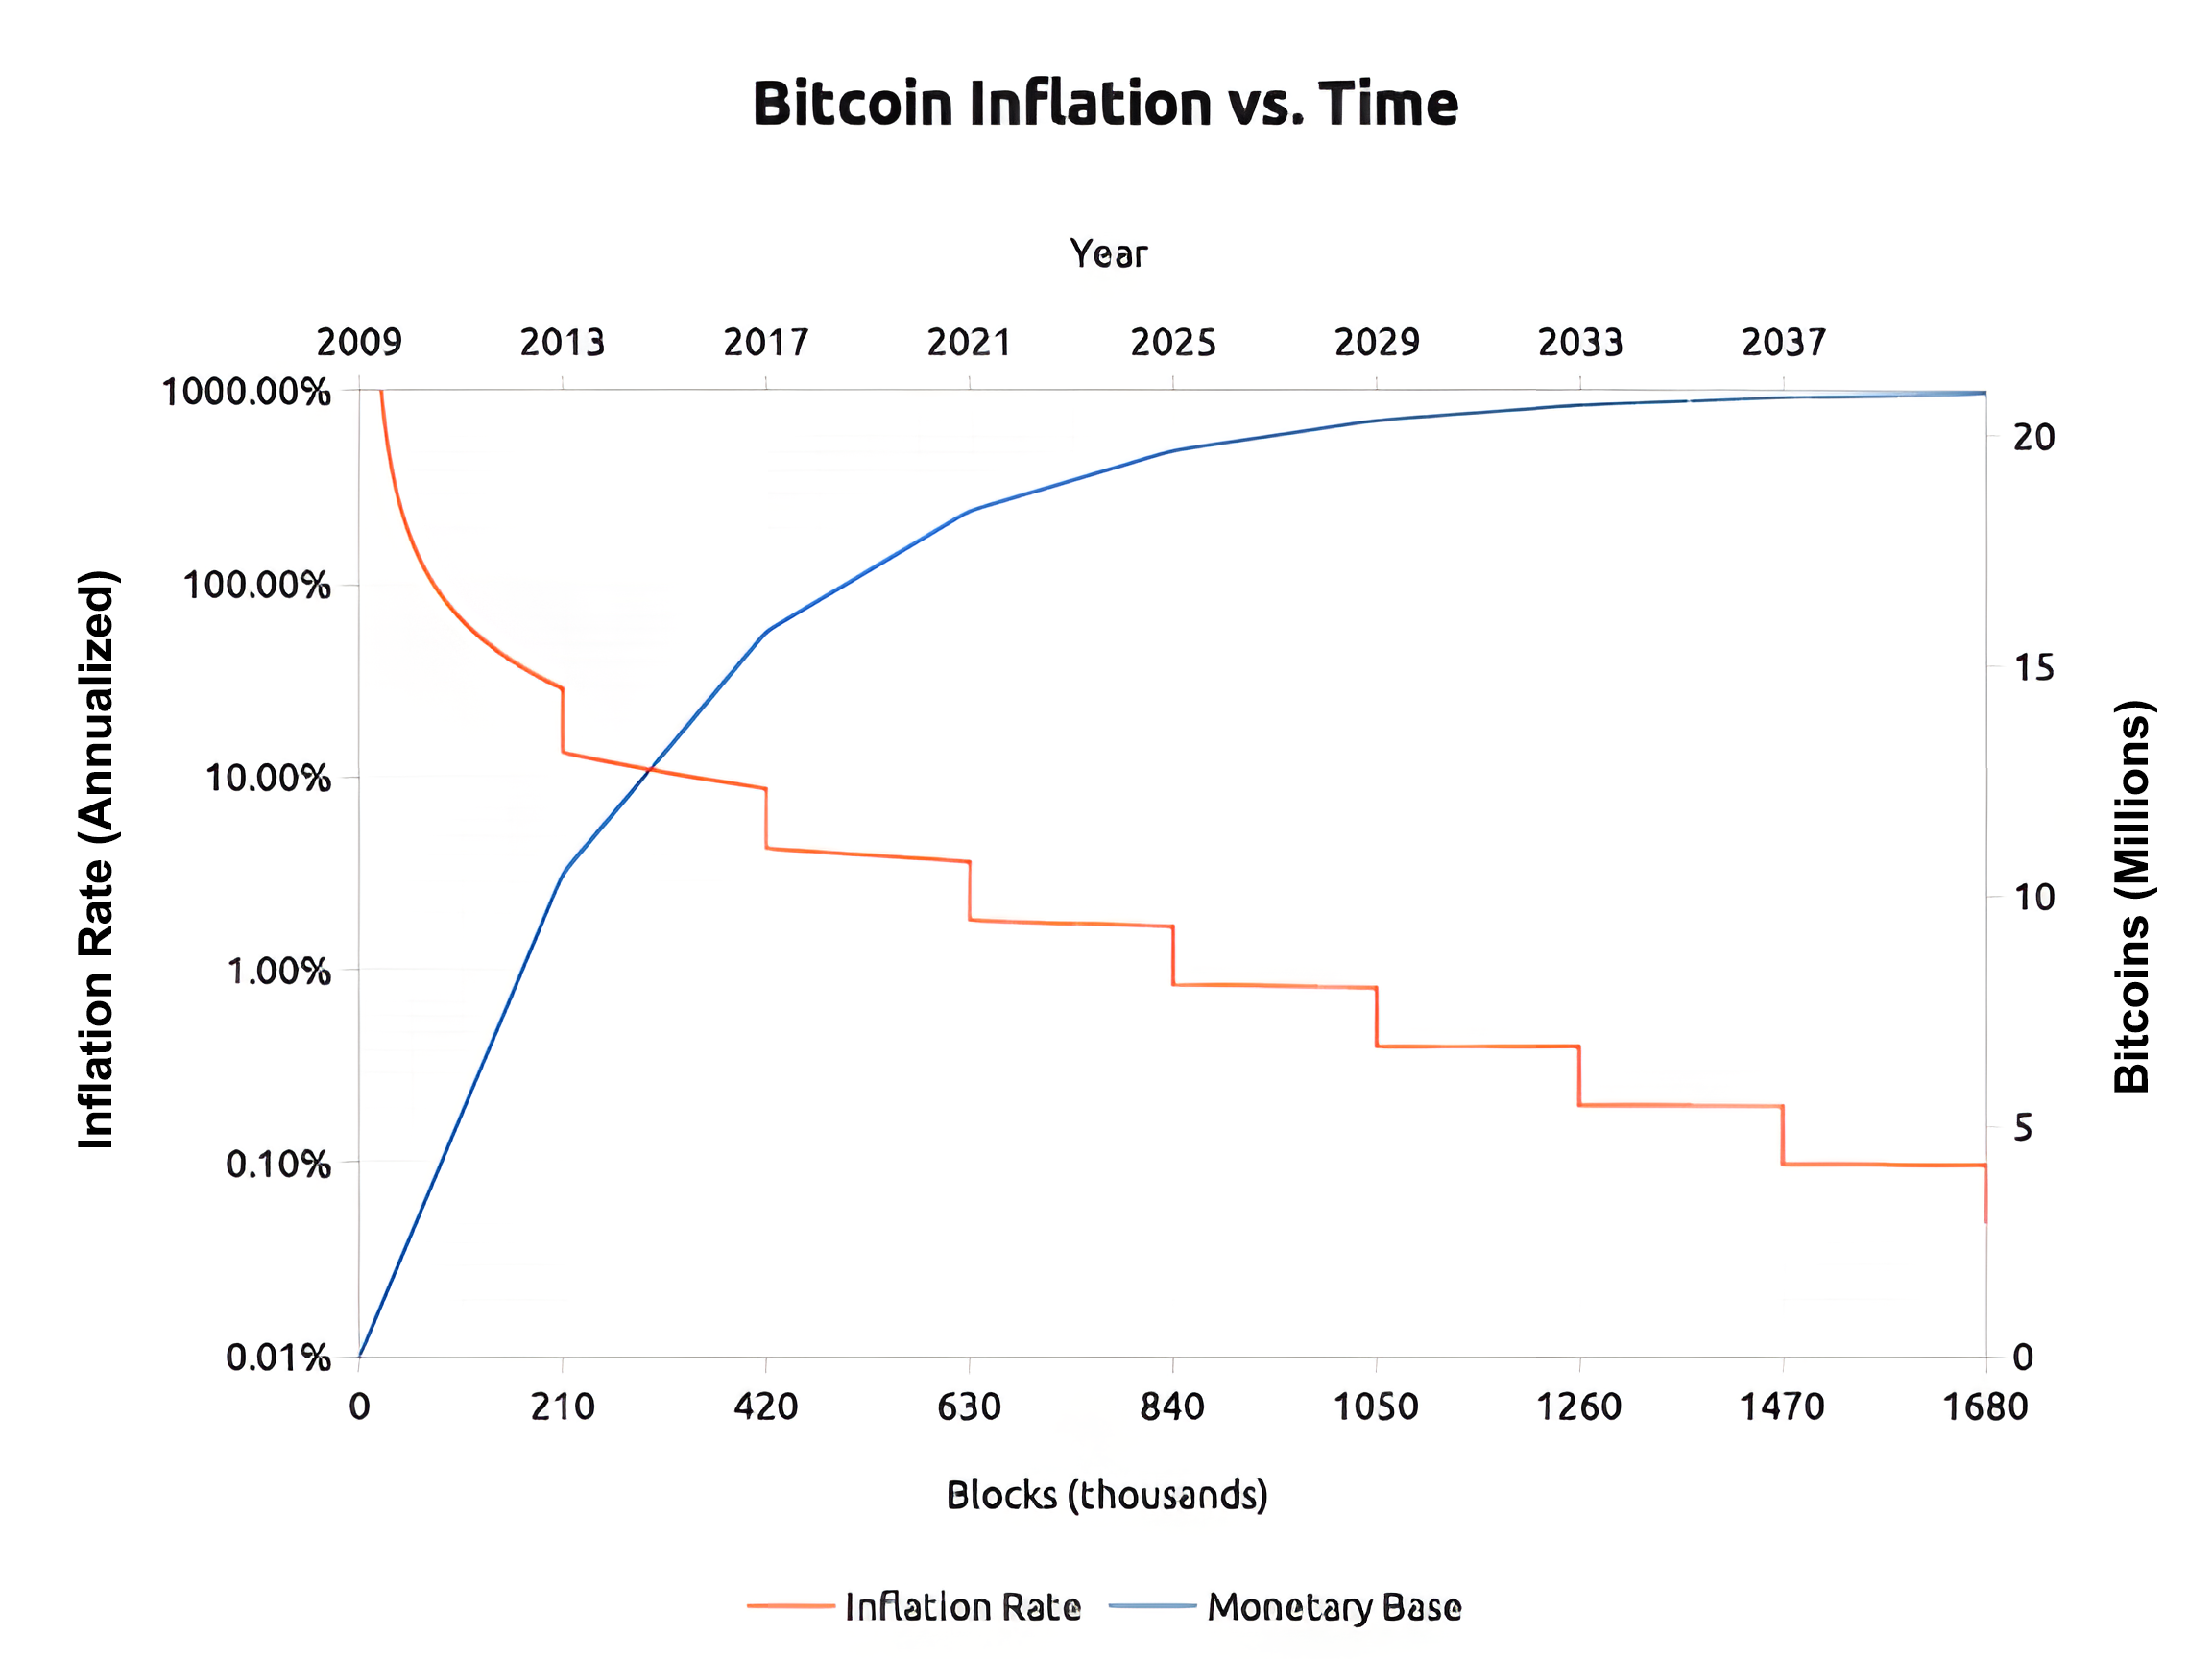
\includegraphics[scale=0.5]{img/matt-whitlock-bitcoin-inflation-log.pdf}
  \caption{Graphique de Matt Whitlock comparant le taux d'émission et la base monétaire du bitcoin en fonction du temps (décembre 2012).}
  \label{fig:bitcoin-inflation}
\end{figure}

L'augmentation de la demande et la diminution du taux de croissance de l'offre entraînent une hausse sensible du prix du bitcoin. Alors qu'il avoisinait les 5~\$ durant la première partie de 2012, il passe à 13~\$ en août et se stabilise à ce niveau jusqu'à la fin de l'année. En 2013, sa progression devient parabolique~: il dépasse les 20~\$ en janvier~; il surmonte l'ancien plus haut des 30~\$ en février~; et il finit par atteindre 266~\$ sur Mt.~Gox en avril.

De façon assez symbolique, un évènement coïncide avec cette hausse~: la faillite des banques chypriotes. À cette époque, la crise financière bat son plein sur l'île de Chypre, ce qui pousse le système financier à prendre des mesures drastiques. Le 16 mars 2013, les banques limitent les retraits des comptes de leurs clients. Le 25, le gouvernement chypriote et l'UE décident (sans cadre légal préalable) que la Bank of Cyprus doit être renflouée de manière interne, via une taxation partielle des dépôts de plus de 100~000~euros. La Laiki Bank, deuxième banque du pays, est démantelée suite à sa faillite et les avoirs supérieurs à 100~000~euros sont tout simplement confisqués. Cet évènement vient démontrer l'utilité du bitcoin, cet «~or numérique~» que l'on peut posséder directement et qui n'est pas soumis aux contraintes des banques à réserves fractionnaires\sendnote{À cette occasion, GoldMoney et Bitcoin Magazine ont co-produit un documentaire, intitulé \eng{Cyprus: A Wake Up Call}, qui recueillait les témoignages des chypriotes touchés par cette crise~: \url{https://bitcoinmagazine.com/culture/cyprus-a-wake-up-call-documentary-by-bitcoin-magazine-and-goldmoney-1365175633}.}.

Du côté de Silk Road, les choses évoluent également. L'enquête des services de renseignement étasuniens, qui a débuté en juin 2011 suite à la publication de l'article d'Adrien Chen sur Gawker et aux injonctions des sénateurs Chuck Schumer et Joe Manchin appelant à fermer la plateforme\pagenote{«~injonctions des sénateurs Chuck Schumer et Joe Manchin appelant à fermer la plateforme~»~: Joe Manchin, \eng{Manchin Urges Federal Law Enforcement to Shut Down Online Black Market for Illegal Drugs}, 6 juin 2011~: \url{https://www.manchin.senate.gov/newsroom/press-releases/manchin-urges-federal-law-enforcement-to-shut-down-online-black-market-for-illegal-drugs}.}, commence à porter ses fruits. Après de longues recherches et quelques actions litigieuses de la part des enquêteurs\sendnote{Deux agents corrompus du FBI ont notamment profité de l'enquête pour subtiliser plus de 20~000~bitcoins (soit environ 350~000~\$) et pour simuler un assassinat. -- Ludovic Lars, \emph{Meurtres, escroqueries et vol de bitcoins - Le côté obscur de Silk Road}, 27 juin 2021~: \url{https://journalducoin.com/analyses/cote-obscur-silk-road/}.}, le fondateur de la plateforme, Ross Ulbricht, finit par être suspecté en juin 2013. C'est Gary Alford, un agent de l'\eng{Internal Revenue Service} (le fisc étasunien), qui débusque la piste en retrouvant l'annonce initiale de Ross sur le forum de Bitcoin et en la liant à son adresse de courriel, où figure son nom civil\pagenote{«~C'est Gary Alford [...] qui débusque la piste~»~: Nathaniel Popper, \eng{The Unsung Tax Agent Who Put a Face on the Silk Road}, 25 décembre 2015~: \url{https://www.nytimes.com/2015/12/27/business/dealbook/the-unsung-tax-agent-who-put-a-face-on-the-silk-road.html}.}. En juillet 2013, le serveur de Silk Road est saisi par la police islandaise et une copie est partagée aux agences étasuniennes\pagenote{«~le serveur de Silk Road est saisi par la police islandaise~»~: \url{https://antilop.cc/sr/files/2014_09_05_Declaration_of_Tarbell.pdf\#page=5}.}. L'historique contient une connexion depuis une adresse IP située à San Francisco, non loin d'où loge le jeune Texan. En septembre, grâce à cette information, Ross est démasqué.

La chute de Silk Road a lieu au début de l'automne 2013. Le 1\ier{} octobre, Ross Ulbricht est maîtrisé par des agents du FBI dans une bibliothèque de San Francisco, avec sa session ouverte sur la plateforme. Le lendemain, le site web est fermé, ce qui provoque l'émoi dans la communauté. Le cours du bitcoin, qui se stabilisait autour des 125~\$ lors des jours précédents, chute brutalement pour toucher un niveau bas de 85~\$. Entre le 2 et le 25 octobre, près de 174~000~bitcoins appartenant à Ross sont saisis par les agences fédérales, un trésor qui représente alors environ 31 millions de dollars\sendnote{29~656,52080180 BTC ont été envoyés à l'adresse \longstring{1F1tAaz5x1HUXrCNLbtMDqcw6o5GNn4xqX} entre le 2 et le 16 octobre, tandis que 144~336,39429472 BTC ont été transférés vers l'adresse \longstring{1FfmbHfnpaZjKFvyi1okTjJJusN455paPH} le 25 octobre. -- U.S. Attorney's Office, Southern District of New York, \eng{Manhattan U.S. Attorney Announces Seizure of Additional \$28 Million Worth of Bitcoins Belonging to Ross William Ulbricht, Alleged Owner and Operator of "Silk Road" Website}, 25 octobre 2013~: \url{https://www.justice.gov/usao-sdny/pr/manhattan-us-attorney-announces-seizure-additional-28-million-worth-bitcoins-belonging}.}.

D'autres personnes liées à Silk Road seront arrêtées et condamnées au cours des années suivantes. Ce sera le cas de Charlie Shrem qui sera interpellé le 27 janvier 2014 par des agents fédéraux (FBI, IRS, DEA) et accusé de facilitation de blanchiment d'argent avec sa société BitInstant. En décembre 2014, il sera condamné à deux ans de prison ferme pour transferts illicites. Ross Ulbricht sera lui condamné à deux peines de réclusion à vie et à 40 ans d'enfermement supplémentaires, pour des charges exclusivement non violentes, dans le but explicite d'en faire un exemple\sendnote{Lors du procès, la juge Katherine Forrest a affirmé~: «~Je rends ce jugement en ayant à l'esprit les crimes que vous avez commis et la nécessité de vous infliger la peine la plus sévère possible. Il ne doit faire aucun doute que le non-respect de la loi ne sera pas toléré. Il ne doit faire aucun doute que personne n'est au-dessus de la loi, quels que soient son éducation ou ses privilèges.~» -- \eng{Ross Ulbricht's sentencing transcript}, 4 février 2015~: \url{https://freeross.org/wp-content/uploads/2018/02/Doc_36_Jan_12_Vol_VI_Appendix_A1314-A1554.pdf\#page=240}.}. % "I make this judgment mindful of the crimes that you have committed and the needs for the severest possible penalty to be imposed. There must be no doubt that lawlessness will not be tolerated. There must be no doubt that no one is above the law, no matter the education or the privileges."

Bien que la chute de Silk Road représente la destruction d'un pan entier de l'économie de Bitcoin, le cours remonte, conformément aux attentes de certains investisseurs importants. L'engouement pour Bitcoin réapparaît, ce qui provoque une nouvelle flambée du prix qui atteint de nouveaux sommets. Celui-ci, s'étant alors stabilisé au-dessus des 100~\$, augmente timidement durant la deuxième moitié d'octobre et dépasse, début novembre, son ancien sommet de 266~\$. À partir de là, il monte en flèche et atteint, le 4 décembre 2013, un nouveau plus haut niveau historique sur Mt.~Gox à 1240~\$. Cet épisode spéculatif pousse alors beaucoup de médias à parler de Bitcoin pour la première fois.

Cependant, la plateforme Mt.~Gox, sur laquelle repose l'essentiel de l'activité spéculative, est beaucoup plus fragile qu'elle ne le paraît. En effet, celle-ci a subi des attaques informatiques tout au long de son existence, entraînant la disparition progressive des fonds. Au début de l'année 2014, il s'avère qu'il manque plus de 650~000~bitcoins dans les caisses de la société, ce qui représente 381 millions de dollars à ce moment-là~!\sendnote{Kim Nilsson, \eng{The missing MtGox bitcoins}, 19 avril 2015~: \url{https://blog.wizsec.jp/2015/04/the-missing-mtgox-bitcoins.html}}

En février 2014, la plateforme Mt.~Gox chute. Après avoir suspendu les retraits le 7, le site est mis hors ligne le 25, et la faillite est déclarée le 28. Mark Karpelès présente ses excuses publiques devant les télévisions japonaises\pagenote{«~Mark Karpelès présente ses excuses publiques devant les télévisions japonaises~»~: \url{https://www.youtube.com/watch?v=NeuCuM9CkBc}}. Cette crise est un cataclysme pour Bitcoin~: la principale plaque tournante de l'économie ferme ses portes, les détenteurs fortunés qui conservaient leurs bitcoins sur la plateforme perdent tout et la confiance du grand public (qui assimile Bitcoin à Mt.~Gox) s'effondre. Cela met fin à l'engouement spéculatif de 2013--2014.

Mark Karpelès est suspecté de détournement de fonds et sa réputation est ternie. Il sera arrêté par la justice japonaise en août 2015, ce qui lui vaudra d'être surnommé le «~baron du bitcoin~» par les médias français\pagenote{«~ce qui lui vaudra d'être surnommé le "baron du bitcoin" par les médias français~»~: Pierre Alonso, \emph{En France, le passé trouble de l'ancien « baron du bitcoin »}, 29 juillet 2014~: \url{https://www.lemonde.fr/pixels/article/2014/08/01/en-france-le-passe-trouble-de-l-ancien-baron-du-bitcoin_4464044_4408996.html}.}. Plus tard, il sera montré que les pertes de la plateforme provenaient de plusieurs piratages ayant eu lieu entre 2011 et 2014, et que Mark Karpelès était seulement coupable de négligence et n'avait pas connaissance de la faille qui a permis de retirer la grosse part des bitcoins entre 2011 et 2014. % En 2019, après un procès éprouvant ayant duré plus d'un an et demi, il sera condamné à 2 ans et demi de prison avec sursis pour manipulation de données informatiques mais acquitté pour l'accusation de détournement de fonds.

Néanmoins, cette chute de Mt.~Gox aura pour effet d'assainir le marché des plateformes d'échange. Dorénavant, elles se partageront le marché de manière plus équitable et l'activité se répartira entre des acteurs comme Bitfinex, bitFlyer, Bitstamp, Bittrex, BTCChina, BTC-e, Coinbase, Gemini, OKEx, Kraken ou encore Poloniex.

\section*{Le débat sur la scalabilité} % 2013 -- 2017
\addcontentsline{toc}{section}{Le débat sur la scalabilité}

% Description générale
La deuxième péripétie qui marque l'histoire de Bitcoin est le débat sur la scalabilité, qui porte sur la capacité du système à passer à l'échelle, c'est-à-dire à continuer de fonctionner de manière équivalente à mesure que le nombre d'utilisateurs augmente. Cette discorde s'amorce au cours de l'année 2013, qui est caractérisée par une forte hausse du prix et de l'activité. Elle dégénère ensuite en une guerre civile en 2015, pour se conclure en 2017 par le schisme en deux communautés distinctes suite à la création d'un nouveau réseau nommé Bitcoin Cash et à l'annulation du projet (artificiel) de compromis SegWit2X. La période constitue une phase d'apprentissage majeure pour la communauté. D'une part, cette dernière prend conscience des imperfections de Bitcoin, qui avait été jusque-là vanté comme un système de monnaie numérique dépourvu d'autorité centrale permettant d'envoyer des paiements instantanés à n'importe qui, n'importe où dans le monde et quasiment sans frais\sendnote{Le 18 mai, la page d'accueil de Bitcoin.org présentait Bitcoin comme un système de monnaie numérique permettant de réaliser des «~transactions instantanées de pair à pair [...] dans le monde entier~» moyennant des «~frais de traitement faibles ou nuls~», en précisant que «~la gestion des transactions et l'émission des bitcoins sont effectuées collectivement par le réseau~». -- \url{https://web.archive.org/web/20130518024528/http://bitcoin.org/en/}.}. D'autre part, la communauté se rend compte du mécanisme de gouvernance qui sous-tend l'évolution du protocole, plus complexe qu'elle n'en a l'air (voir chapitres~\ref{ch:changement} et \ref{ch:determination}).

% "Bitcoin is a digital currency, a protocol, and a software that enables instant peer-to-peer transactions, worldwide payments, low or zero processing fees. Bitcoin uses peer-to-peer technology to operate with no central authority or banks; managing transactions and the issuing of bitcoins is carried out collectively by the network. Bitcoin is open-source; its design is public, nobody owns or controls Bitcoin and everyone can take part. Through many of its unique properties, Bitcoin allows exciting uses that could not be covered by any previous payment system."
%
% « Le bitcoin est une monnaie numérique, un protocole et un logiciel qui permet des transactions instantanées de pair à pair, des paiements dans le monde entier et des frais de traitement faibles ou nuls. Bitcoin utilise la technique pair-à-pair pour fonctionner sans autorité centrale ni banque ; la gestion des transactions et l'émission des bitcoins sont effectuées collectivement par le réseau. Bitcoin est un logiciel libre ; sa conception est publique, personne ne possède ou ne contrôle Bitcoin et tout le monde peut y participer. Grâce à ses nombreuses propriétés uniques, le bitcoin permet des utilisations passionnantes qui ne pouvaient être couvertes par aucun système de paiement antérieur. »

Le débat sur la scalabilité se concentre sur un paramètre présent dans le protocole qui restreint la capacité transactionnelle du système~: la limite de la taille des blocs ou \eng{blocksize limit}. Puisque dans Bitcoin, les transactions sont incluses dans des blocs qui sont ajoutés à la chaîne toutes les 10 minutes en moyenne, limiter la taille de ces blocs revient en effet à instaurer un quota sur le nombre de transactions confirmées.

En 2013, la taille limite est de 1~mégaoctet (1~Mo), ce qui correspond à un flux théorique maximal de 7,37~transactions par seconde. Ajoutée dans le protocole par Satoshi Nakamoto le 12 septembre 2010 sans annonce publique de sa part, cette limite avait initialement pour rôle d'empêcher les attaques par déni de service et devait être augmentée au fil du temps\sendnote{Le 4 octobre 2010, Satoshi décrivait sur le forum comment mettre en œuvre une augmentation de la taille limite des blocs. -- Satoshi Nakamoto, \eng{Re: [PATCH] increase block size limit}, \wtime{04/10/2010 19:48:40 UTC}, \url{https://bitcointalk.org/index.php?topic=1347.msg15366\#msg15366}).}. Néanmoins, après la disparition précipitée du fondateur, la décision a été laissée aux membres de la communauté, ce qui a préparé le terrain pour le conflit.

Dans le débat, deux camps principaux se font face. Le premier est celui des partisans des gros blocs, ou \eng{big blockers}, qui se réclament du projet initial de Satoshi, et qui désirent réaliser des mises à niveau pour accroître la limite, voire la supprimer. Le camp opposé est celui des partisans des petits blocs, ou \eng{small blockers}, qui souhaitent restreindre la taille des blocs, afin de minimiser le coût de gestion d'un nœud.

La première vision, qui est au départ majoritaire, considère que l'augmentation progressive de la taille limite des blocs peut être réalisée sans mettre en danger l'intégrité du système. Cette vision estime que Bitcoin devrait rester un protocole de paiement, qui s'adapte à la demande sans hausse des frais de transactions. Elle favorise de ce fait la facilité d'utilisation par rapport à la sécurité. Elle accepte le recours aux \eng{hard forks}, mises à niveau incompatibles du protocole qui demandent la coordination de tous les membres du réseau pour être réalisées proprement. Il s'agit d'une position plutôt progressiste. De plus, ses partisans jugent généralement que la détermination du protocole est assurée par les mineurs. % logique des gros blocs

Cette approche est notamment portée par les développeurs Gavin Andresen, Mike Hearn et Jeff Garzik.

La seconde vision, qui se développe à partir de 2013, se concentre sur la sécurité aux dépens de la facilité d'utilisation. Son but est de minimiser le coût de gestion d'un nœud afin de maximiser la décentralisation du réseau. Cette vision considère que Bitcoin doit être principalement un protocole de règlement, servant de base à des systèmes en surcouche, qui peuvent être centralisés ou décentralisés. Elle prône l'utilisation de \eng{soft forks}, des mises à niveau du protocole rendues rétrocompatibles grâce à l'action des mineurs, et qui peuvent donc être adoptées progressivement par les utilisateurs. Il s'agit d'une position plutôt conservatrice, même si elle admet l'intervention de certains changements essentiels. En outre, ses partisans considèrent généralement que l'intégrité du protocole provient des utilisateurs.  % logique des petits blocs

Cette approche est notamment soutenue par les développeurs Pieter Wuille, Gregory Maxwell, Wladimir van der Laan et luke-jr.

Dans ces deux camps, il existe des nuances et des contradictions. Le sujet de la scalabilité étant complexe et technique, toutes sortes de positions émergent, notamment sur le niveau auquel devrait être fixé la limite de la taille des blocs~: 1~Mo, 2~Mo, 8~Mo~?

L'opposition entre les deux tendances se manifeste tout d'abord au sein du projet logiciel de Bitcoin, dont les contributeurs principaux sont majoritairement des partisans des petits blocs. Durant le printemps 2014, le logiciel connaît ainsi un tournant majeur. Au niveau de la forme d'abord, il est renommé «~Bitcoin Core~» le 19 mars dans le but de «~réduire la confusion entre Bitcoin-le-réseau et Bitcoin-le-logiciel\sendnote{Bitcoin Core, \eng{Bitcoin Core version 0.9.0 released}, 19 mars 2014~: \url{https://bitcoin.org/en/release/v0.9.0\#rebranding-to-bitcoin-core}.}~». Puis en ce qui concerne le fond, le dépôt GitHub subit une passation de pouvoir le 7 avril lorsque Gavin Andresen cède son poste de mainteneur principal à Wladimir van der Laan, pour se consacrer à ses activités de scientifique en chef de la Fondation Bitcoin.

Ce changement de gestion se matérialise dans l'année, lorsque Mike Hearn voit sa proposition d'ajout de la requête de réseau \longstring{getutxos} être rejetée pour cause de non-unanimité dans l'équipe de Bitcoin Core\pagenote{«~Mike Hearn voit sa proposition d'ajout de la requête de réseau getutxos être rejetée pour cause de non-unanimité dans l'équipe de Bitcoin Core~»~: \url{https://github.com/bitcoin/bitcoin/commit/70352e11c0194fe4e71efea06220544749f4cd64}.}. L'ingénieur, a besoin de cette fonctionnalité pour le développement de son application de financement participatif, Lighthouse. De ce fait, il est contraint de créer Bitcoin XT en décembre 2014, une implémentation alternative issue de Bitcoin Core qui inclut les changements désirés mais qui reste compatible avec le réseau\pagenote{«~il est contraint de créer Bitcoin XT en décembre 2014~»~: Mike Hearn, \eng{[Bitcoin-development] Bitcoin XT}, \wtime{28/12/2014 18:04:08 UTC}~: \url{https://lists.linuxfoundation.org/pipermail/bitcoin-dev/2014-December/007057.html}.}.

Simultanément, la discorde s'étend à l'ensemble de la communauté. La logique des petits blocs se diffuse en particulier grâce à une vidéo produite par le développeur Peter Todd en 2013, qui explique «~pourquoi la taille limite des blocs permet à Bitcoin de rester libre et décentralisé\sendnote{Keep Bitcoin Free, \eng{Why the blocksize limit keeps Bitcoin free and decentralized}, 17 mai 2013~: \url{https://www.youtube.com/watch?v=cZp7UGgBR0I}.}~». Un autre argument invoqué est celui du marché des frais, notamment mis en valeur par l'économiste français Nicolas Houy, qui explique dans un article de 2014 que «~laisser les frais de transaction résulter d'un marché et rendre la taille des blocs non pertinente ou non contraignante conduirait à un niveau de sécurité trop faible pour Bitcoin\sendnote{Nicolas Houy, \eng{The economics of Bitcoin transaction fees}, 2014. -- Cette idée, appelée la «~spirale fatale des frais~», avait été proposée dès 2011 par un utilisateur sur Bitcointalk. Voir Vandroiy, \eng{[If tx limit is removed] Disturbingly low future difficulty equilibrium}, 22 avril 2011~: \url{https://bitcointalk.org/index.php?topic=6284.msg92187\#msg92187}.}~». Enfin, les partisans des petits blocs cherchent à justifier leur point de vue en proposant des solutions de passage à l'échelle, permettant d'accroître l'activité économique soutenue par le réseau sans pour autant augmenter significativement la taille des blocs.

La première est la proposition des chaînes latérales, ou \eng{pegged sidechains}, qui sont des chaînes secondaires fonctionnant en parallèle de la chaîne principale, vers et depuis lesquelles des bitcoins peuvent être transférés grâce à un ancrage bilatéral. Cette proposition est présentée pour la première fois dans un document technique le 22 octobre 2014 par les développeurs de l'entreprise Blockstream. Co-fondée par Adam Back, des développeurs de Bitcoin Core et des personnalités de la finance, cette société dont la création est annoncée le même jour a pour but de «~trouver une manière d'étendre l'utilisation de Bitcoin, qui soit architecturalement solide et qui ne nécessite pas d'autorisation, pour que la cryptomonnaie atteigne son plein potentiel\sendnote{Blockstream, \eng{Why We Founded Blockstream}, 22 octobre 2014~: \url{https://web.archive.org/web/20161022162335/https://www.blockstream.com/2014/10/23/why-we-are-co-founders-of-blockstream.html}.}~». Elle se focalisera dans un premier temps sur le développement des sidechains, ce qui donnera naissance au modèle Elements et à sa mise en œuvre, Liquid.

% Adam Back, Pieter Wuille, Gregory Maxwell, Matt Corallo, Jorge Timón, Mark Friedenbach, ainsi que Erik Svenson, Austin Hill, Jonathan Wilkins, Francesca Hall, Alex Fowler

La seconde proposition est celle du réseau Lightning, ou \eng{Lightning Network}, un réseau de canaux de paiements bâti en surcouche de Bitcoin permettant d'effectuer des transferts instantanés et quasi-gratuits de pair à pair. Le concept est présenté en février 2015 par Joseph Poon et Thaddeus Dryja lors d'un séminaire de développeurs à San Francisco. Le 28 février, ils publient le livre blanc de leur invention, qui est intitulé «~\eng{The Bitcoin Lightning Network}~» et qui présente les éléments de base nécessaires pour construire un tel réseau\sendnote{Joseph Poon et Thaddeus Dryja, \eng{The Bitcoin Lightning Network DRAFT Version 0.5}, 28 février 2015~: \url{https://lightning.network/lightning-network-paper-DRAFT-0.5.pdf}.}. En particulier, une implémentation fluide de Lightning demande de modifier le protocole Bitcoin par l'ajout de verrous temporels dans le langage de script et par la correction d'un défaut appelé la malléabilité des transactions\sendnote{La malléabilité des transactions est la possibilité de modifier légèrement une transaction après sa diffusion sur le réseau, de façon à changer son identifiant. Cette capacité disparaît cependant une fois que la transaction a été confirmée par un mineur qui l'a incluse dans un bloc de la chaîne.}.

Ces deux propositions font envisager un passage à l'échelle par surcouche, qui ne nécessiterait pas de s'en remettre totalement à un tiers de confiance et qui ne compromettrait pas la sécurité de la chaîne toute entière.

Du côté des partisans des gros blocs, on se concentre surtout sur l'optimisation du logiciel et du protocole afin d'alléger la charge des nœuds. Ainsi, le 6 octobre 2014, Gavin Andresen publie une feuille de route sur le blog de la Fondation Bitcoin dans laquelle il décrit la façon dont les effets de l'augmentation de l'activité du réseau pourraient être compensés par des changements du protocole et par l'évolution exponentielle de la technique décrite par les lois de Moore et de Nielsen\sendnote{Gavin Andresen, \eng{A Scalability Roadmap}, 6 octobre 2014~: \url{https://web.archive.org/web/20150321091124/http://blog.bitcoinfoundation.org:80/a-scalability-roadmap}.}. L'article mentionne notamment l'élagage des blocs les plus anciens (\eng{block pruning}) qui permettrait de diminuer la taille de la chaîne à conserver, l'«~engagement des UTXO~» ayant pour but d'accélérer le téléchargement initial des blocs, ou encore le relai des blocs par \eng{Invertible Bloom Lookup Tables} qui serait plus efficace.

Au printemps 2015, la taille moyenne des blocs approchant des 500~ko, l'idée d'augmenter la capacité transactionnelle du réseau est remise sur le devant de la scène sous l'impulsion de Gavin Andresen qui publie une série d'articles à ce sujet sur son blog personnel\pagenote{«~Gavin Andresen [...] publie une série d'articles à ce sujet sur son blog personnel~»~: Gavin Andresen, \eng{Time to roll out bigger blocks}, 4 mai 2015~: \url{http://gavinandresen.ninja/time-to-roll-out-bigger-blocks}.}. Dans les mois qui suivent, plusieurs propositions apparaissent, notamment celle de Gavin d'augmenter la limite à 8~Mo (BIP-101), conformément aux vœux des coopératives minières chinoises, et celle de Pieter Wuille d'augmenter cette limite de 17,7~\% par an (BIP-103). Malheureusement aucune proposition ne satisfait les forces en présence. Cela a pour effet d'intensifier le conflit au sein de la communauté, qui dégénère alors en une véritable guerre civile.

\section*{La guerre des blocs} % 2015 -- 2017
\addcontentsline{toc}{section}{La guerre des blocs}

Le conflit sur la taille des blocs prend un tournant majeur au cours de l'été 2015, avec la sortie de la version 0.11A de Bitcoin XT le 15 août, qui inclut une augmentation de la limite de la taille des blocs, changement incompatible avec les règles du réseau\sendnote{Mike Hearn, \eng{Why is Bitcoin forking?}, 15 août 2015~: \url{https://medium.com/faith-and-future/why-is-bitcoin-forking-d647312d22c1}.}. La mise à niveau intégrée est le BIP-101 qui programme un passage de la limite de 1 à 8~Mo, à condition d'atteindre un signalement suffisant des mineurs, à savoir 75~\% de la puissance de calcul du réseau. De ce fait, cette version du logiciel a la possibilité de créer une séparation du réseau et une scission de la chaîne en deux chaînes distinctes.

L'implémentation Bitcoin XT est dirigée par Mike Hearn qui se décrit comme un «~dictateur bienveillant~» (concept courant dans le monde du logiciel libre). Gavin Andresen participe au projet et a son mot à dire sur la direction prise, mais «~Mike prend les décisions finales en cas de litiges graves\sendnote{\eng{FAQ -- BitcoinXT} (archive)~: \url{https://web.archive.org/web/20150908031806/https://bitcoinxt.software/faq.html\#who-is-involved}.}~». L'augmentation de la taille limite des blocs est soutenue par les grandes coopératives minières chinoises\pagenote{«~L'augmentation de la taille limite des blocs est soutenue par les grandes coopératives minières chinoises~»~: \eng{Why upgrade to 8MB but not 20MB?}, 12 juin 2015~: \url{https://www.reddit.com/r/Bitcoin/comments/3a0n4m/why_upgrade_to_8mb_but_not_20mb/}.} et par une partie des entreprises de l'industrie\pagenote{«~et par une partie des entreprises de l'industrie~»~: \eng{Industry Letter Regarding Block Size}, 24 août 2015~: \url{https://blog.bitmex.com/wp-content/uploads/2017/09/industry-letter.pdf}.}.

Ce mouvement ressemble grandement à un passage en force aux yeux d'un noyau dur de la communauté, ce qui ne manque pas de provoquer sa réaction épidermique. Dans la nuit du 16 au 17 août, Michael Macquart (alias theymos), le modérateur principal du subreddit r/Bitcoin et co-gestionnaire du forum Bitcointalk, publie ainsi un long article sur Reddit dans lequel il annonce interdire toutes les discussions à propos de Bitcoin XT\sendnote{Michael Macquart, \eng{It's time for a break: About the recent mess \& temporary new rules}, \wtime{17/08/2015 00:50:15}~: \url{https://www.reddit.com/r/Bitcoin/comments/3h9cq4/its_time_for_a_break_about_the_recent_mess/}.}. Dans cet article, il explique en particulier pourquoi il considère que Bitcoin XT ne peut pas être Bitcoin, et que les échanges à son sujet n'ont par conséquent pas leur place sur le subreddit. Puisque l'essentiel des conversations se passe sur r/Bitcoin à l'époque, cette décision a un impact non négligeable.

L'apparition de Bitcoin XT marque donc le début d'une guerre civile au sein de la communauté, que l'on appellera la guerre des blocs ou la \eng{blocksize war}\sendnote{Le terme anglais est issu de l'ouvrage \eng{The Blocksize War} de Jonathan Bier publié en 2021. Le terme français a été inventé par Morgan Phuc en 2017~: \url{https://bitconseil.fr/bitcoin-guerre-blocs/}.}, au cours de laquelle la diplomatie fait progressivement place à l'animosité. Dans la journée du 17 août, le journaliste Alex Hern écrit dans le Guardian~: «~La guerre des bitcoins a commencé.\sendnote{Alex Hern, \eng{Bitcoin's forked: chief scientist launches alternative proposal for the currency}, 17 août 2015~: \url{https://www.theguardian.com/technology/2015/aug/17/bitcoin-xt-alternative-cryptocurrency-chief-scientist}.}~» Celle-ci sera marquée par une forte propagande des deux côtés, par la censure sur les principaux canaux de communication\pagenote{«~la censure sur les principaux canaux de communication~»~: John Blocke, \eng{A (brief and incomplete) history of censorship in /r/Bitcoin}, 14 novembre 2016~: \url{https://medium.com/@johnblocke/a-brief-and-incomplete-history-of-censorship-in-r-bitcoin-c85a290fe43}.} et par des attaques par déni de service contre les nœuds utilisant Bitcoin XT et ses successeurs\pagenote{«~des attaques par déni de service contre les nœuds utilisant Bitcoin XT et ses successeurs~»~: Deryk Makgill, \eng{Cyber Attacks Against Scaling Bitcoin}~: \url{https://wakgill.github.io/deryk/bitcoin-cyber-attacks}.}.

Toutefois, au début, beaucoup cherchent à apaiser le conflit et appellent à la discussion. C'est le but des conférences appelées \eng{Scaling Bitcoin}, organisées pour présenter les différentes manières de faire passer Bitcoin à l'échelle. La première édition se déroule en septembre à Montréal et parvient à réunir des individus des deux camps dans une bonne foi partagée. Le deuxième édition a lieu en décembre à Hong Kong, où la tension est déjà plus palpable.

Durant \eng{Scaling Bitcoin II}, une nouvelle proposition pour Bitcoin est présentée~: Segregated Witness ou, plus simplement, SegWit. Imaginée par Gregory Maxwell et Pieter Wuille, celle-ci prévoit de faciliter l'implémentation du réseau Lightning (en corrigeant la malléabilité des transactions) et d'augmenter la capacité transactionnelle de façon rétrocompatible pour les nœuds non miniers. Elle fait partie de la feuille de route de Gregory Maxwell publiée le même jour sur la liste de diffusion\sendnote{Gregory Maxwell, \eng{[bitcoin-dev] Capacity increases for the Bitcoin system}, \wtime{07/12/2015 22:02:17 UTC}~: \url{https://lists.linuxfoundation.org/pipermail/bitcoin-dev/2015-December/011865.html}.} et devient rapidement la mise à niveau défendue par les partisans des petits blocs.

Au début de l'année 2016, Bitcoin XT échoue et Mike Hearn quitte la communauté dans un abandon rageur retentissant\sendnote{Mike Hearn, \eng{The resolution of the Bitcoin experiment}, 14 janvier 2016~: \url{https://blog.plan99.net/the-resolution-of-the-bitcoin-experiment-dabb30201f7}.}. Cependant, une nouvelle implémentation émerge du côté des partisans des gros blocs~: Bitcoin Classic. Celle-ci intègre une version modifiée du BIP-101 qui porterait une taille limite de 2~Mo en cas d'un signalement de 75~\% de la puissance de calcul du réseau. Bitcoin Classic gagne rapidement en popularité au point d'interpeler le camp opposé\sendnote{«~Bitcoin Classic a émergé des cendres du débat entre XT et Core. Il s'agit d'une version de Bitcoin qui autoriserait une limite de deux mégaoctets, mettant en place des règles pour l'augmenter au cours du temps. Elle semble gagner rapidement du soutien.~» -- Paul Vigna, \eng{Is Bitcoin Breaking Up?}, 17 janvier 2016~: \url{https://web.archive.org/web/20160117220315/https://www.wsj.com/articles/is-bitcoin-breaking-up-1453044493}.}.

Le 20 février 2016, une réunion d'urgence est organisée à Hong Kong. Cette «~Table Ronde~» réunit les principales coopératives minières, certaines entreprises de l'écosystème et des contributeurs majeurs de Bitcoin Core, dont Matt Corallo, Peter Todd ou encore luke-jr. Après de nombreuses heures de discussions sous pression, les participants arrivent à une entente, que l'on appellera l'accord de Hong Kong. D'un côté, les développeurs de Bitcoin Core s'engagent à implémenter SegWit et un doublement de la limite de la taille de base des blocs. De l'autre, les mineurs s'engagent à activer SegWit et à n'utiliser que Bitcoin Core\sendnote{Bitcoin Roundtable, \eng{Bitcoin Roundtable Consensus}, 20 février 2016~: \url{https://medium.com/@bitcoinroundtable/bitcoin-roundtable-consensus-266d475a61ff}.}.

Mais ce sentiment de compromis ne dure pas, car l'année 2016 amène deux évènements qui changent la donne. Le premier est l'intervention de Craig Wright, un informaticien et entrepreneur australien qui prétend être Satoshi Nakamoto. Il est propulsé sur le devant de la scènes en décembre 2015 suite à la publication de deux enquêtes indépendantes par Wired et Gizmodo, selon lesquelles il serait probablement le créateur de Bitcoin\pagenote{«~deux enquêtes indépendantes par Wired et Gizmodo, selon lesquelles il serait probablement le créateur de Bitcoin~»~: Andy Greenberg, Gwern Branwen, \eng{Bitcoin's Creator Satoshi Nakamoto Is Probably This Unknown Australian Genius}, 8 décembre 2015 (\url{https://web.archive.org/web/20151208214655/https://www.wired.com/2015/12/bitcoins-creator-satoshi-nakamoto-is-probably-this-unknown-australian-genius/})~; Sam Biddle and Andy Cush, \eng{This Australian Says He and His Dead Friend Invented Bitcoin}, 8 décembre 2015 (\url{https://web.archive.org/web/20151208235451/https://gizmodo.com/this-australian-says-he-and-his-dead-friend-invented-bi-1746958692}).}. Ces enquêtes se basent sur des éléments pouvant en effet laisser penser qu'il a été impliqué dans la conception de la cryptomonnaie aux côtés de son ami Dave Kleiman, mort en 2013.

Quelques mois plus tard, le 2 mai 2016, Craig Wright publie un long et tortueux article de blog\sendnote{Craig Wright, \eng{Jean-Paul Sartre, Signing and Significance}, 2 mai 2016~: \url{https://web.archive.org/web/20160502072011/http://www.drcraigwright.net/jean-paul-sartre-signing-significance/}.}, dans lequel il inclut une signature correspondant à la clé publique utilisée pour recevoir la récompense du bloc 9 et envoyer le premier paiement à Hal Finney en janvier 2009. En outre, un entretien de Craig Wright avec la BBC est mis en ligne ce jour-là, dans lequel l'Australien affirme avoir été «~l'élément principal~» derrière Satoshi Nakamoto, mais que «~d'autres personnes l'ont aidé\sendnote{BBC News, \eng{Mr Bitcoin: "I don't want money, I don't want fame!"}, 2 mai 2016~: \url{https://www.youtube.com/watch?v=5DCAC1j2HTY}.}~». Il prétend également avoir signé un message en privé devant le journaliste qui l'interroge.

Cependant, il s'avère que les documents fournis dans les enquêtes et les éléments avancés par Craig Wright lui-même ne sont pas probants. En particulier, on découvre très rapidement que la signature présente dans l'article de blog est la signature d'une transaction existante sur la chaîne de Bitcoin qui est simplement encodée différemment\sendnote{La signature fournie par Craig Wright correspond à la clé publique liée à l'adresse \longstring{12cbQLTFMXRnSzktFkuoG3eHoMeFtpTu3S} qui a servi à recevoir la récompense du bloc 9 et à envoyer le premier paiement à Hal Finney le 12 janvier 2009, et a donc été produite par Satoshi Nakamoto. Néanmoins, un utilisateur de Reddit (JoukeH) a découvert très rapidement qu'il s'agissait de la signature d'une transaction présente sur la chaîne~:\url{https://www.reddit.com/r/Bitcoin/comments/4hf4xj/creator_of_bitcoin_reveals_identity/d2pf70v/}.}. Ce fait incite la communauté à la prudence.

Le même jour, Gavin Andresen publie un article dans lequel il dit croire que Craig Wright est «~la personne qui a inventé Bitcoin~», ce dernier lui ayant présenté en personne «~des messages signés avec les clés que seul Satoshi devrait posséder\sendnote{Gavin Andresen, \eng{Satoshi}, 2 mai 2016~: \url{http://gavinandresen.ninja/satoshi}}~». En conséquence, le rôle de mainteneur et le \eng{commit access} de Gavin sur le dépôt de Bitcoin Core sont révoqués dans la foulée, sous prétexte que les membres de l'équipe de Bitcoin Core craignent qu'il ait été piraté. De manière générale, cette affirmation douteuse, confirmée en personne le jour-même lors de la conférence Consensus 2016, a pour effet de le discréditer et son accès au dépôt GitHub ne sera jamais restauré. Il reconnaîtra plus tard avoir été dupé\pagenote{«~Il reconnaîtra plus tard avoir été dupé~»~: \emph{Déposition de Gavin Andresen dans le cadre de l'affaire Wright / Kleiman}, 19 juin 2020~: \url{https://storage.courtlistener.com/recap/gov.uscourts.flsd.521536/gov.uscourts.flsd.521536.589.3.pdf\#page=88}.}.

Le second évènement qui vient influencer le conflit est un incident qui ne se passe pas au sein de la communauté de Bitcoin, mais sur Ethereum, un système alternatif à Bitcoin dédié aux \eng{smart contracts} lancé en 2015. Il s'agit de la scission entre Ethereum (ETH) et Ethereum Classic (ETC) qui fait suite au piratage de TheDAO. % 20 juillet 2016

Le 17 juin 2016, le contrat de TheDAO, une organisation autonome décentralisée ayant pour mission d'investir dans l'écosystème, est piraté et 3,6 millions d'éthers (l'éther est l'unité de compte d'Ethereum) valant 50 millions de dollars sont dérobés, ce qui représente 4,4 \% de la quantité totale d'éthers en circulation à l'époque. La décision est alors prise par une grande majorité de la communauté d'annuler purement et simplement ce vol par la modification de l'état du système. Un mois plus tard, le 20 juillet, le changement est appliqué ce qui conduit à une scission de la chaîne en deux chaînes distinctes~: celle suivant le protocole modifié (qui est majoritaire et qui prendra le nom d'Ethereum) et celle suivant le protocole initial (qui est minoritaire et qui s'appellera Ethereum Classic). Les détenteurs se retrouvent avec des éthers différents des deux côtés.

Cette séparation n'est pas propre. En particulier, elle n'inclut pas de protection contre la rediffusion des transactions, ce qui signifie que des transferts réalisés sur une chaîne peuvent être répliqués sur l'autre par un tiers, menant à des «~attaques par rediffusion~» (\eng{replay attacks}). Cela perturbe les plateformes d'échange qui doivent composer avec ce problème. Ainsi, même si le prix combiné des deux éthers finit par être supérieur au prix de l'éther initial, tout le monde peut observer les effets négatifs d'une scission créée par un hard fork. Cet exemple conforte de ce fait la position conservatrice des partisans des petits blocs qui recommandent de faire évoluer le protocole par des soft forks tels que SegWit.

À cause de ces deux évènements, le camp des partisans des gros blocs ressort de cette année 2016 particulièrement diminué, tant au niveau réputationnel qu'argumentatif.

C'est ce moment que choisissent les développeurs de Bitcoin Core pour lancer le signalement de SegWit par les mineurs, qui commence le 15 novembre 2016, pour une période d'un an\pagenote{«~lancer le signalement de SegWit par les mineurs, qui commence le 15 novembre 2016~»~: Bitcoin Core, \eng{Bitcoin Core version 0.13.1 released}, 27 octobre 2016~: \url{https://bitcoin.org/en/release/v0.13.1\#segregated-witness-soft-fork}.}. La mise à niveau exige un taux de signalement de 95~\% de la puissance de calcul pour être activée, dans le but d'assurer largement la rétrocompatiblité du changement.

Cependant, les principales coopératives minières refusent SegWit (pour des raisons multiples\sendnote{SegWit annulait notamment les effets de l'AsicBoost secret, une technique d'optimisation du minage. Cf. Gregory Maxwell, \eng{[bitcoin-dev] BIP proposal: Inhibiting a covert attack on the Bitcoin POW function}, \wtime{05/04/2017 21:37:45 UTC}~: \url{https://lists.linuxfoundation.org/pipermail/bitcoin-dev/2017-April/013996.html}.}) et, durant les premiers mois, le taux de blocs en faveur de la mise à niveau stagne autour des 25~\%, très loin du seuil demandé. SegWit est bloqué.

Au début de l'année 2017, les blocs commencent à être pleins, ce qui engendre une augmentation significative des frais de transaction et des temps de confirmation sur la chaîne. Mi-février, les frais médians dépassent les 30 centimes de dollar, pour la première fois dans l'histoire de Bitcoin. C'est dans ce contexte que la demande pour un changement s'accroît de part et d'autre du conflit.

D'un côté, nous avons Bitcoin Unlimited, une implémentation qui a gagné en popularité chez les partisans des gros blocs lors de l'été 2016 et qui a pris la relève de Bitcoin Classic. Celle-ci est notamment soutenue par Roger Ver, le PDG de l'entreprise Bitcoin.com qui est alors devenu une personnalité influente de la communauté\sendnote{Roger Ver est connu pour son prosélytisme de l'adoption du bitcoin dans le commerce et pour sa participation éclatante au documentaire \eng{The Bitcoin Gospel} diffusé le 1\ier{} novembre 2015 sur Youtube (\url{https://www.youtube.com/watch?v=8zKuoqZLyKg&t=2831s}).}, ce qui permet à Bitcoin Unlimited de disposer d'un large financement. En mars 2017, le signalement pour Unlimited dépasse ainsi celui de SegWit.

Cependant, le 17 mars, la possibilité d'un hard fork contentieux pousse les plateformes d'échange à considérer la potentielle monnaie créée par Bitcoin Unlimited comme une cryptomonnaie alternative. Fortes de leur expérience avec la scission entre ETH et ETC, elles exigent en outre qu'elle intègre une protection contre la rediffusion, faute de quoi elle ne sera même pas listée\pagenote{«éelles exigent en outre qu'elle intègre une protection contre la rediffusion, faute de quoi elle ne sera même pas listée~»~: Aaron van Wirdum, \eng{Major Exchanges Will Consider Bitcoin Unlimited a "New Asset"}, 17 mars 2017~:\url{https://bitcoinmagazine.com/technical/major-exchanges-will-consider-bitcoin-unlimited-new-asset}}. Cette décision est dévastatrice pour les partisans des gros blocs.

De l'autre côté, la pression en faveur de l'activation de SegWit s'intensifie au sein des partisans des petits blocs, qui commencent à devenir impatients. Ainsi, le 12 mars 2017, un individu se faisant appeler Shaolin Fry publie la proposition d'un UASF («~\eng{User Activated Soft Fork}~») qui permettrait de verrouiller la mise à niveau sans le signalement des mineurs dès le 1\ier{} août\sendnote{Shaolin Fry, \eng{[bitcoin-dev] Flag day activation of segwit}, \wtime{12/03/2017 15:50:27 UTC}~: \url{https://lists.linuxfoundation.org/pipermail/bitcoin-dev/2017-March/013714.html}.}. Cette mesure, pour le moins audacieuse, est dangereuse et ne fait pas l'unanimité parmi les \eng{small blockers}, comme l'illustre l'opposition de Gregory Maxwell\pagenote{«~l'opposition de Gregory Maxwell~»~: Gregory Maxwell, \eng{[bitcoin-dev] I do not support the BIP 148 UASF}, \wtime{14/04/2017 07:56:31 UTC}~: \url{https://lists.linuxfoundation.org/pipermail/bitcoin-dev/2017-April/014152.html}.}.

Cependant, la menace de l'UASF existe et exerce une influence. Ainsi, devant le désir de la communauté de procéder à SegWit, les gros acteurs de l'écosystème (entreprises et mineurs) sont amenés à signer un accord le 23 mai 2017, en marge de la conférence Consensus 2017 à New York. Cet accord de New York, comme on l'appellera par la suite, représente un compromis théorique dans le conflit qui fait rage~: il engage les signataires, d'une part, à activer SegWit avec un seuil de signalement de 80~\% de la puissance de calcul, d'autre part, à doubler la taille limite des blocs dans les six mois qui suivent. La mise à niveau implémentant cet accord prendra le nom de SegWit2X. Ce pseudo-compromis est néanmoins rapidement critiqué en raison de l'absence des développeurs de Bitcoin Core à la réunion, qui n'étaient tout simplement pas conviés.

L'accord mène à l'activation de SegWit durant l'été 2017. En juillet, les mineurs commencent à signaler massivement la mise à niveau. Le 21, le processus de verrouillage est enclenché (ce qui rend l'UASF ineffectif). SegWit finit par être activé le 24 août 2017.

La mise à niveau se passe très bien. Cependant, il se produit au même moment une autre scission, pleinement désirée. En opposition à l'UASF, les mineurs décident d'activer un nouveau protocole, incompatible avec le protocole originel, qui n'intègre pas SegWit et qui implémente une taille limite des blocs de 8~Mo~: Bitcoin Cash. Le lancement de ce protocole est placé sous l'autorité d'Amaury Séchet, un développeur français.

Le 1\ier{} août 2017, avec le bloc 478~559 miné à 18 heures 12, naît ainsi Bitcoin Cash. À la suite de cette scission, les détenteurs de bitcoin se retrouvent avec un montant similaire en bitcoins (BTC) et en bitcoins cash (BCH). Ceux qui désapprouvent SegWit rejoignent Bitcoin Cash.

Durant le mois d'août, alors que SegWit est enfin verrouillé, certains partisans des petits blocs commencent à s'opposer à la deuxième partie de SegWit2X, le doublement de la taille des blocs, via une campagne de communication baptisée «~NO2X~». Dans leur argumentaire, ils insistent en particulier sur l'absence de rediffusion des transactions que comporte ce hard fork\pagenote{«~ils insistent en particulier sur l'absence de rediffusion des transactions~»~: Alex Bosworth, \eng{[Bitcoin-segwit2x] Alpha Milestone}, \wtime{14/06/2017 17:35:00 UTC}~: \url{https://lists.linuxfoundation.org/pipermail/bitcoin-segwit2x/2017-June/000003.html}.}. En effet, SegWit2X est pensé comme un changement non contentieux et n'inclut par conséquent pas ce type de procédé qui alourdirait considérablement la charge de la mise à jour pour les portefeuilles.

L'opposition gronde. Les développeurs de Bitcoin Core refusent d'approuver ce changement. Les utilisateurs se mobilisent pour protester, car «~la manière dont l'accord a été conclu va à l'encontre de l'essence même de Bitcoin\sendnote{Change.org, \emph{Nous nous opposons au New York Agreement et au hard fork Bitcoin SegWit2X de novembre.}, 15 octobre 2017~: \url{https://www.change.org/p/mineurs-et-entreprises-de-l-éco-système-bitcoin-nous-nous-opposons-au-new-york-agreement-et-au-hard-fork-bitcoin-segwit2x-de-novembre}.}~». Face à cette opposition, les entreprises signataires de l'accord de New York se rétractent peu à peu.

Le projet de doublement de la limite de la taille des blocs est finalement abandonné le 8 novembre 2017, soit une semaine avant son activation programmée. Les promoteurs du projet -- Mike Belshe, Wences Casares, Jihan Wu, Jeff Garzik, Peter Smith et Erik Voorhees -- déclarent conjointement~:

\begin{quote}
«~Notre objectif a toujours été d'améliorer Bitcoin en douceur. Bien que nous croyons fermement en la nécessité d'augmenter la taille des blocs, il y a une chose que nous croyons encore plus importante~: garder la communauté unie. Malheureusement, il est clair que nous n'avons pas recueilli un consensus suffisant à l'heure actuelle pour une modification propre de la taille des blocs. Continuer sur la voie actuelle pourrait diviser la communauté et constituer un revers pour la croissance de Bitcoin. Cela n'a jamais été l'objectif de Segwit2x.\sendnote{Mike Belshe, \eng{[Bitcoin-segwit2x] Segwit2x Final Steps}, \wtime{08/11/2017 16:58:41 UTC}~: \url{https://lists.linuxfoundation.org/pipermail/bitcoin-segwit2x/2017-November/000685.html}.}~»
\end{quote}

C'est une grande victoire pour la philosophie des petits blocs qui dominera dorénavant la chaîne. Pour ce qui est des solutions de scalabilité sur BTC, le réseau Lightning est lancé en version bêta en mars 2018. Le concept de chaîne latérale est également expérimenté, avec le lancement de Rootstock en janvier 2018 et celui de la sidechain Liquid développée par Blockstream en septembre de la même année.

De l'autre bord, suite à l'annulation de SegWit2X, beaucoup de partisans de l'augmentation de la capacité de la chaîne se dirigent vers d'autres protocoles comme Bitcoin Cash ou Ethereum.

Malgré le dénigrement constant de ses détracteurs, l'évolution de Bitcoin Cash suivra son cours. Néanmoins, sa communauté se délitera progressivement et la cryptomonnaie connaîtra deux scissions majeures avec la création de Bitcoin SV en novembre 2018 puis celle de «~eCash~» (XEC) en novembre 2020. La valeur agrégée du BCH représente \textcolor{darkgray}{aujourd'hui moins de 1~\% de celle du BTC}.

\section*{L'essor des cryptomonnaies alternatives}
\addcontentsline{toc}{section}{L'essor des cryptomonnaies alternatives}

Bitcoin est un projet libre~: il se base sur un code source ouvert qui peut être copié et déployé sur un nouveau réseau par n'importe qui. Cette particularité est excellente pour l'innovation~: un individu, quel qu'il soit, peut apporter des modifications au code et en faire la base d'une nouvelle cryptomonnaie s'il le désire. La découverte de Bitcoin ouvre ainsi la voie à une vraie concurrence des monnaies sur Internet. Cependant, cette liberté existe aussi pour les personnes mal intentionnées qui peuvent profiter de cette ouverture pour créer des projets douteux, allant de la cryptomonnaie inutile à l'escroquerie pure et simple, en passant par la pyramide de Ponzi ouverte. C'est dans cette dualité entre l'honnêteté de l'innovateur et la cupidité du malfaiteur que se produit l'essor de ce qu'on appelle les «~cryptomonnaies alternatives~» («~\eng{altcoins}~» en anglais).

La première idée d'une cryptomonnaie distincte de Bitcoin apparaît alors que Satoshi est encore présent dans la communauté. En novembre 2010, une discussion sur un système distribué de noms de domaine (alors appelé BitDNS) s'engage sur IRC, puis sur le forum de Bitcoin\pagenote{«~une discussion sur un système distribué de noms de domaine (alors appelé BitDNS) s'engage sur IRC, puis sur le forum de Bitcoin~»~: appamatto, \eng{BitDNS and Generalizing Bitcoin}, \wtime{15/11/2010 03:02:31 UTC}~: \url{https://bitcointalk.org/index.php?topic=1790.msg22019\#msg22019}.}. Il s'agit d'associer des identifiants de site web (DNS) à des pièces créées par le protocole, comme les bitcoins dans Bitcoin. Le registre étant public et difficilement falsifiable, cela améliorerait les choses par rapport au système existant. Satoshi n'est pas hostile à l'idée et suggère de miner la chaîne en combinaison (\eng{merge mining}) avec celle de Bitcoin\sendnote{Satoshi Nakamoto, \eng{Re: BitDNS and Generalizing Bitcoin}, \wtime{09/12/2010 21:02:42 UTC}~: \url{https://bitcointalk.org/index.php?topic=1790.msg28696\#msg28696}.}. Cela donne finalement naissance à Namecoin en avril 2011, créé sous l'impulsion de Vincent Durham\pagenote{«~Cela donne finalement naissance à Namecoin~»~: Vincent Durham (vinced), \eng{[announce] Namecoin - a distributed naming system based on Bitcoin}, \wtime{18/04/2011 00:52:59 UTC}~: \url{https://bitcointalk.org/index.php?topic=6017.msg88356\#msg88356}.}.

Par la suite, d'autres cryptomonnaies apparaissent, comme Ixcoin ou Tenebrix. Tenebrix a la particularité d'implémenter l'algorithme de preuve de travail scrypt, mis au point par le mineur ArtForz et supposément résistant aux processeurs graphiques. En octobre 2011, Litecoin est lancé par Charlie Lee, en tant que «~version allégée de Bitcoin~» dont les blocs sont minés quatre fois plus rapidement, dont l'unité de compte est quatre fois moins rare et qui intègre l'algorithme scrypt. Litecoin a pour but d'être «~à l'argent ce que Bitcoin est à l'or\sendnote{Charlie Lee (coblee), \eng{Re: [ANN] Litecoin - a lite version of Bitcoin. Be ready when is launches!}, \wtime{09/10/2011 06:14:28 UTC}~: \url{https://bitcointalk.org/index.php?topic=47417.msg564414\#msg564414}.}~».

En août 2012, Sunny King et Scott Nadal lancent PPCoin, un système introduisant le procédé de preuve d'enjeu, qu'ils présentent comme une alternative à la preuve de travail «~économe en énergie à long terme\sendnote{Sunny King, \eng{[ANN] [PPC] PPCoin Released! - First Long-Term Energy-Efficient Crypto-Currency}, \wtime{19/08/2012 19:54:28 UTC}~: \url{https://bitcointalk.org/index.php?topic=101820.msg1113938\#msg1113938}~; Sunny King, Scott Nadal, \eng{PPCoin: Peer-to-Peer Crypto-Currency with Proof-of-Stake}, 19 août 2012, archive~: \url{https://web.archive.org/web/20121021014644/http://www.ppcoin.org/static/ppcoin-paper.pdf}.}~». Le preuve d'enjeu est intégrée de manière hybride aux côtés de la preuve de travail. PPCoin sera progressivement renommé en Peercoin au cours des années.

% XRP (août 2012)

En 2013, avec l'engouement financier résultant du succès du bitcoin, la création de cryptomonnaies originales devient extrêmement rentable. Les nouveaux protocoles se multiplient à l'instar de Feathercoin en avril, de Primecoin en juillet ou encore du célèbre Dogecoin en décembre\pagenote{«~du célèbre Dogecoin en décembre~»~: Ludovic Lars, \eng{Le dogecoin est-il un concurrent sérieux au bitcoin~?}, 1\ier{} mai 2021~: \url{https://www.contrepoints.org/2021/05/01/396380-le-dogecoin-est-il-un-concurrent-serieux-au-bitcoin}.}. Le site web coinmarketcap.com est créé en mai 2013 pour recenser l'ensemble des cryptomonnaies et les classer par «~capitalisation boursière~», c'est-à-dire par leur valeur agrégée (le nombre d'unités multiplié par le prix unitaire).

Cependant, ce foisonnement n'est pas du goût de tout le monde et un mouvement de rejet se forme face à ce qui ressemble à une fragmentation dommageable de l'écosystème. Dès 2011, on voit un certain scepticisme se développer vis-à-vis des premières cryptomonnaies alternatives, scepticisme qui transparaît dans les réactions de Hal Finney et de Gavin Andresen\pagenote{«~scepticisme qui transparaît dans les réactions de Hal Finney et de Gavin Andresen~»~: Hal Finney, \eng{Re: Early speculators' reward}, \wtime{30/05/2011 18:28:34 UTC}~: \url{https://bitcointalk.org/index.php?topic=10666.msg152988\#msg152988}~; Gavin Andresen, \eng{Alternative Block Chains~: be safe!}, \wtime{09/09/2011 13:21:18 UTC}~: \url{https://bitcointalk.org/index.php?topic=42465.msg516789\#msg516789}.}. Puis, le rejet devient plus tranché en août 2013 avec les prises de positions de Gavin Andresen (encore lui), qui assimile la création de nouvelles cryptomonnaies à de l'inflation\sendnote{Gavin Andresen, \eng{The macro-economics of alt-coins}, 19 août 2013~: \url{https://gavintech.blogspot.com/2013/08/the-macro-economics-of-alt-coins.html}.}, et de Daniel Krawisz, auteur pour le Satoshi Nakamoto Institute, qui met en lumière la difficulté extrême de surpasser l'effet de réseau de Bitcoin\sendnote{Daniel Krawisz, \eng{The Problem with Altcoins}, 22 août 2013~: \url{https://nakamotoinstitute.org/mempool/the-problem-with-altcoins/}.}.

En parallèle, on assiste à la formation de la tendance contraire~: un pluralisme cryptomonétaire qui prône l'ouverture et la tolérance envers cette diversité des cryptomonnaies. Celui-ci est en particulier défendu par le jeune Vitalik Buterin en septembre 2013\sendnote{Vitalik Buterin, \eng{In Defense of Alternative Cryptocurrencies}, 7 septembre 2013~: \url{https://bitcoinmagazine.com/business/defense-alternative-cryptocurrencies}.}, qui le mettra en pratique avec l'élaboration de son propre projet, Ethereum.

À partir de 2014, cette tendance est renforcée par l'apparition de systèmes cryptoéconomiques fondamentalement plus pertinents que les simples copies de Bitcoin. Ainsi, pour corriger le manque de confidentialité de la chaîne de blocs de Bitcoin, plusieurs solutions voient le jour. C'est le cas de Darkcoin qui démarre en janvier 2014 (et qui deviendra plus tard Dash). Monero, un protocole intégrant la confidentialité par défaut dont le nom signifie «~pièce de monnaie~» en esperanto, est lui lancé en avril. En outre, la publication des protocoles Zerocoin et Zerocash par Matthew Green en 2013 mèneront à la création de Zcash en octobre 2016.

Mais la confidentialité n'est pas le seul terrain d'innovation, et d'autres protocoles séparés émergent pour mettre en œuvre un perfectionnement de l'aspect programmable de Bitcoin, conformément à l'idée d'un «~Bitcoin 2.0~» qui se diffuse alors dans la communauté. En effet, le protocole de Satoshi est peu adapté pour réaliser des opérations complexes et créer des jetons numériques secondaires, même si cela peut se faire sur des surcouches comme Omni et Counterparty. C'est pourquoi on assiste à la naissance de nouveaux systèmes, à l'instar de Bitshares, une place de marché décentralisée qui a la particularité de fonctionner par preuve d'enjeu déléguée, et de NXT, une plateforme incluant un grand nombre de fonctionnalités\pagenote{«~NXT, une plateforme incluant un grand nombre de fonctionnalités~»~: Bas Wisselink, \eng{| Nxt | Blockchain Platform | Proof of Stake | Official}, \wtime{27/04/2014 19:01:37 UTC}~: \url{https://bitcointalk.org/index.php?topic=587007.msg6426512\#msg6426512}.}. Mais le système qui se distingue le plus est Ethereum.

Ethereum reprend la programmabilité de Bitcoin et la généralise en constituant une sorte d'ordinateur mondial décentralisé, fonctionnant en parallèle sur tous les nœuds d'un réseau pair-à-pair. Ce projet est, comme on l'a dit, issu de l'esprit de Vitalik Buterin, qui en dresse les contours à la fin de l'année 2013. Avec ses 7 co-fondateurs, il réalise une prévente de jetons en juillet-août 2014, qui recueille 31 529 bitcoins\sendnote{L'adresse BTC utilisée par EthSuisse était \longstring{36PrZ1KHYMpqSyAQXSG8VwbUiq2EogxLo2}. -- Vitalik Buterin, \eng{Launching the Ether Sale}, 22 juillet 2014~: \url{https://blog.ethereum.org/2014/07/22/launching-the-ether-sale}.} (soit plus de 15 millions de dollars à l'époque) pour en financer le développement. Ethereum est un système volontairement plus progressiste, plus innovant et plus flexible que Bitcoin. La chaîne sera officiellement lancée un an plus tard, le 30 juillet 2015.

L'année 2014 est enfin l'année où apparaît le premier \eng{stablecoin}, le Tether USD (ou USDT), qui est lancé sur la chaîne de Bitcoin le 6 octobre sous le nom de Realcoin\pagenote{«~le Tether USD [...] est lancé sur la chaîne de Bitcoin le 6 octobre sous le nom de Realcoin~»~: \url{https://www.omniexplorer.info/tx/5ed3694e8a4fa8d3ec5c75eb6789492c69e65511522b220e94ab51da2b6dd53f}.}. Ce jeton numérique est adossé au dollar grâce à la garantie de l'entreprise Tether Limited, qui s'engage à racheter chaque unité contre un dollar réel. Cette cryptomonnaie «~stable~» permet aux individus et aux plateformes d'échange de bénéficier de la faible volatilité du dollar, sans avoir à en subir les inconvénients légaux.

Face à ce développement, le mouvement de rejet à l'égard de ces nouveaux projets continue de croître. Il s'illustre le 22 octobre 2014 par la publication du document de Blockstream sur les sidechains, qui vient décrire comment Bitcoin pourrait être à la base de tous les cas d'utilisation, et d'un article, expliquant la démarche derrière la fondation de la société. Dans ce dernier, les développeurs travaillant pour Blockstream écrivent ainsi~:

\begin{quote}
«~L'approche des altcoins, qui consiste à créer une nouvelle cryptomonnaie uniquement pour introduire de nouvelles fonctionnalités, crée une incertitude pour tous ceux qui observent les cryptomonnaies de l'extérieur. Il ne semble pas y avoir de point d'arrêt naturel, chaque copie pouvant être copiée à nouveau, à l'infini. Cela crée à la fois une fragmentation du marché et une fragmentation du développement. Nous pensons que pour que les cryptomonnaies réussissent dans leur ensemble, nous devons construire de l'effet de réseau, et non de la fragmentation.\sendnote{Blockstream, \eng{Why We Founded Blockstream}, 22 octobre 2014~: \url{https://web.archive.org/web/20161022162335/https://www.blockstream.com/2014/10/23/why-we-are-co-founders-of-blockstream.html}.}~»
\end{quote}

Au fil des années, ce rejet prend progressivement le nom de maximalisme du bitcoin (\eng{bitcoin maximalism}), par réappropriation du terme utilisé péjorativement par Vitalik Buterin à l'encontre de ceux qui dénigrent systématiquement les cryptomonnaies alternatives\sendnote{L'expression utilisée par Vitalik Buterin est «~\eng{bitcoin dominance maximalist}~», qu'on peut traduire par «~maximaliste de la dominance du bitcoin~» (\url{https://www.reddit.com/r/Bitcoin/comments/2is4us/whats_wrong_with_counterparty/cl54c0y/}). Dans son article publié le 19 novembre 2014, il définit le maximalisme du bitcoin comme «~l'idée qu'un milieu de multiples cryptomonnaies concurrentes est indésirable, qu'il est mal de lancer "encore un autre jeton", et qu'il est à la fois juste et inévitable que la monnaie bitcoin en vienne à atteindre une position de monopole sur la scène des cryptomonnaies~» (Vitalik Buterin, \eng{On Bitcoin Maximalism, and Currency and Platform Network Effects}, 19 novembre 2014~: \url{https://blog.ethereum.org/2014/11/20/bitcoin-maximalism-currency-platform-network-effects/})}. Le mouvement prône la maximisation de la dominance économique du bitcoin par rapport à ses concurrents proches et prescrit à ses partisans d'agir dans ce sens. Il s'agit de mettre en valeur l'effet de réseau, non seulement parce que c'est techniquement nécessaire mais aussi parce que c'est moralement désirable\sendnote{L'appartenance au maximalisme est parfois revendiquée aujourd'hui par des gens qui n'embrassent pas son caractère extrémiste (même s'il se trouve dans le terme). C'est pourquoi on peut recourir au pléonasme «~maximalisme toxique~» pour désigner cette tendance. Jameson Lopp parle aussi de «~puritanisme du bitcoin~» dans son \eng{History of Bitcoin Maximalism} publiée le 25 mars 2023~: \url{https://blog.lopp.net/history-of-bitcoin-maximalism/}.}.

% Pierre Rochard, Michael Goldstein, Tone Vays, Giacomo Zucco, Francis Pouliot, Aleksandar Svetski. 

Cependant, devant les limites de Bitcoin mises en exergue durant la guerre des blocs, le phénomène de substitution des autres systèmes cryptoéconomiques va en s'intensifiant au fur et à mesure du temps. Ainsi à partir de mars 2017, la dominance du BTC par rapport aux autres cryptomonnaies décroche du niveau des 85~\% où elle se maintenait jusqu'alors pour rejoindre les 40~\% en juin. Cela vient en particulier de l'essor d'Ethereum, qui constitue un moyen simple d'émettre des jetons programmables sur sa chaîne de blocs. Cette fonctionnalité permet notamment de lever des fonds en réalisant une prévente de jetons, nommée \eng{Initial Coin Offering} ou ICO, pour financer des projets dans lesquels interviendront les jetons en question. Le nombre de levées de fonds de ce type explose en 2017 -- 2018, à tel point que l'on parle de «~folie des ICO~». La plus importante d'entre elles, celle d'EOS, lève 4,1 milliards de dollars sur une période d'un an.

% En conséquence, le prix de l'éther passe d'une poignée de dollars début 2017 à plus de 1400~\$ en janvier 2018.

En 2019, un autre enthousiasme se dessine~: celui de la finance décentralisée, appelée \eng{decentralized finance} ou DeFi en anglais. L'objectif de la DeFi est de reproduire les outils du système financier traditionnel de manière numérique, décentralisée, ouverte et transparente. Il s'agit de minimiser l'intermédiation (souvent de manière imparfaite) intervenant dans l'exécution de diverses opérations financières~: les échanges, le prêt sur gage (aussi appelé crédit lombard), la création de produits dérivés, les marchés prédictifs,~etc. Ce développement a principalement lieu sur Ethereum et est notamment incarné par l'émergence du protocole Maker qui permet l'existence du premier stablecoin décentralisé~: le dai. Dans la DeFi, le BTC est utilisé comme un collatéral de premier choix. À côté de cela, il se crée une nouvelle mode autour des jetons non fongibles ou NFT (pour \eng{non-fongible tokens}), un engouement qui finit par toucher le grand public à partir de 2021.

Cependant, tous ces projets souffrent de failles techniques et humaines parfois très importantes, de sorte que la critique reste pertinente. À certains projets, il manque bien souvent la fameuse «~décentralisation~» qu'ils prétendent posséder. D'autres sont des doublons, qui n'apportent rien et disparaissent à cause de l'effet de réseau de leurs concurrents. D'autres enfin sont tout simplement des escroqueries, dans le sens où leurs promoteurs principaux mentent pour vendre leur jeton. Tout ceci explique pourquoi le maximalisme du bitcoin subsiste encore à l'écriture de ces lignes.

\section*{L'intégration institutionnelle} % 2017 -- 2022
\addcontentsline{toc}{section}{L'intégration institutionnelle}

L'ouverture à la finance traditionnelle initiée en 2012 se traduit au fil du temps par une intégration dans le système légal existant. Cette tendance est naturelle~: pour que Bitcoin existe, il doit jouir d'une certaine tolérance de la part de la population et, \emph{in fine}, des autorités qui «~représentent~» cette dernière.

L'institutionnalisation passe en premier lieu par la réglementation (ou «~régulation~») du secteur, qui consiste à l'assujettir à un cadre légal généralement défini et appliqué par l'État. En pratique, il s'agit de soumettre les acteurs financiers importants à des normes plus ou moins drastiques. La réglementation est donc synonyme de contrôle, chose à quoi Bitcoin s'oppose fondamentalement, d'où la tension qui en découle.

% La réglementation, aussi désignée par l'anglicisme « régulation », est l'acte d'assujettir une activité sociale à un règlement, une prescription ou une loi. Elle provient généralement d'une contrainte légale appliquée par l'État. Pour la cryptomonnaie et le domaine financier en général, il s'agit de soumettre les acteurs importants à des normes plus ou moins drastiques. La réglementation est donc synonyme de contrôle, chose à quoi Bitcoin s'oppose fondamentalement, d'où la tension qui en découle.

Dès les premières années d'existence de Bitcoin, les agences de renseignement s'y intéressent, aux États-Unis comme en France. Ainsi, en avril 2011, la CIA invite Gavin Andresen à venir parler de Bitcoin, chose qu'il fait en juin. Le 9 mai 2012, un rapport interne du FBI sur Bitcoin fuite sur Internet~: on peut y lire que «~si Bitcoin se stabilise et gagne en popularité, il deviendra un outil de plus en plus utile pour diverses activités illégales au-delà du cyberespace\sendnote{Kim Zetter, \eng{FBI Fears Bitcoin's Popularity with Criminals}, 9 mai 2012~: \url{http://www.wired.com/2012/05/fbi-fears-bitcoin/}.}~». En juillet 2012, un rapport de Tracfin dit que les «~monnaies virtuelles~» posent un «~risque spécifique en matière de lutte contre le blanchissement des capitaux et le financement du terrorisme\sendnote{Tracfin, \emph{Rapport d'activité 2011}, juillet 2012~: \url{https://www.economie.gouv.fr/files/files/directions_services/tracfin/Publications/rapports_activite/2011_rapport_FR.pdf}}~».

Ces enquêtes préparent la réglementation financière qui se met en place à partir de 2013, sous l'effet de la hausse du cours du printemps. C'est ainsi que, le 18 mars, le FinCEN (\eng{Financial Crimes Enforcement Network}) publie un document clarifiant sa position sur les monnaies numériques\sendnote{Financial Crimes Enforcement Network, \eng{Application of FinCEN's Regulations to Persons Administering, Exchanging, or Using Virtual Currencies}, 18 mars 2013, \url {https://www.fincen.gov/sites/default/files/shared/FIN-2013-G001.pdf}.}. Il spécifie dans celui-ci que les plateformes de change sont des entreprises de services monétaires (\eng{money services business}) et doivent par conséquent obtenir une licence pour exercer aux États-Unis.

Peu à peu, les normes se durcissent. Les plateformes se mettent à appliquer une procédure de connaissance du client (appelée en anglais \eng{Know Your Customer} ou KYC) en imposant une vérification d'identité pour accéder à leurs services. Elles peuvent également aller plus loin dans le cadre de la «~lutte contre le blanchiment des capitaux et le financement du terrorisme~» (LCB-FT).

D'autres réglementations financières s'appliquent aux cryptomonnaies, comme la taxation des plus-values. En France par exemple, l'utilisateur est légalement contraint de déclarer ses plus-values réalisées lors des «~cessions à titre onéreux d'actifs numériques~» et de payer un impôt de 30~\% sur celles-ci, si le total des ventes représente plus de 305~€ sur l'année\sendnote{Code général des impôts, \emph{Article 150 VH bis}, 24 mai 2019.}. % https://www.legifrance.gouv.fr/codes/article_lc/LEGIARTI000038612228/

La réglementation diffère cependant entre les juridictions. Et si certaines sont clémentes, d'autres le sont beaucoup moins. C'est par exemple le cas de l'État de New York qui, en 2015, fait passer une réglementation ultra-restrictive, imposant à une large part des acteurs de l'écosystème d'obtenir une licence d'exploitation appelée la «~BitLicence~»\pagenote{«~une réglementation ultra-restrictive, imposant à une large part des acteurs de l'écosystème d'obtenir une licence d'exploitation appelée la "BitLicence"~»~: Davis Polk, \eng{New York's Final "BitLicense" Rule: Overview and Changes from July 2014 Proposal}, 5 juin 2015~: \url{https://www.davispolk.com/sites/default/files/2015-06-05_New_Yorks_Final_BitLicense_Rule.pdf}.}. Dans le même esprit, l'État français fait passer un décret en novembre 2019 pour assujettir les prestataires de services sur actifs numériques (PSAN) à des conditions strictes\pagenote{«~l'État français fait passer un décret en novembre 2019~»~: \emph{Décret n° 2019-1213 du 21 novembre 2019 relatif aux prestataires de services sur actifs numériques}~: \url{https://www.legifrance.gouv.fr/loda/id/JORFTEXT000039407517/}.}. Dans les deux cas, cela a pour effet de faire fuir les acteurs locaux vers des juridictions plus accomodantes.

Outre cette réglementation, le discours des acteurs traditionnels est au départ ouvertement hostile à la conception originelle de Bitcoin. On peut le voir en 2014 -- 2015 avec l'apparition du terme «~\eng{blockchain technology}~», dont le but caché est de nier le côté rebelle de la cryptomonnaie, en amalgamant l'ensemble des techniques de consensus distribué au sein d'une même appellation. Cet appel à la blockchain est popularisé en 2015 par Blythe Masters, une ancienne opératrice de marché de JPMorgan Chase, connue pour avoir conçu les contrats de couverture de défaillance (CDS), à l'origine de la crise des subprimes\sendnote{Edward Robinson et Matthew Leising, \eng{Blythe Masters Tells Banks the Blockchain Changes Everything}, 1\ier{} septembre 2015~:\url{https://www.bloomberg.com/news/features/2015-09-01/blythe-masters-tells-banks-the-blockchain-changes-everything}.}. Cependant, le discours s'adoucit au fur et à mesure que les années passent. % https://web.archive.org/web/20150901181219/https://www.bloomberg.com/news/features/2015-09-01/blythe-masters-tells-banks-the-blockchain-changes-everything % Elle permet aux institutions financières de ne pas parler de Bitcoin, qui a alors encore mauvaise presse. C'est le début du discours «~\eng{Blockchain, not Bitcoin}~», qui séduira pendant un temps le monde financier traditionnel.

La réglementation amène ainsi de nouvelles contraintes, en opposition frontale au principe d'absence d'autorisation intrinsèquement lié à Bitcoin. Mais elle permet peu à peu à de plus gros investisseurs, comme les fonds d'investissement, d'entrer sur le marché avec de la liquidité, de légitimer la cryptomonnaie aux yeux du grand public, qui a besoin d'une approbation officielle pour oser s'y intéresser. Cela pousse ainsi certains acteurs de la communauté à chercher à coopérer avec le régulateur. % En outre, il se greffe à la réglementation en soi un processus de domestication, d'adoucissement, d'\emph{aseptisation} de l'objet, qui vient cacher voire son côté rebelle.

En 2017, un nouvel engouement spéculatif apparaît, durant lequel le prix du bitcoin connaît une forte hausse en passant de 1000~\$ en janvier à 20~000~\$ en décembre. Cette nouvelle bulle attire à nouveau l'attention des médias. Bitcoin est désormais pris beaucoup plus au sérieux. En décembre 2017, il entre même à la bourse de Chicago pour faire l'objet d'un contrat à terme, ce qui correspond à une avancée notable\pagenote{«~En décembre 2017, il entre même à la bourse de Chicago~»~: Grégory Raymond, \eng{Le bitcoin débarque à la Bourse de Chicago : un moment historique !}, 8 décembre 2017~: \url{https://www.capital.fr/crypto/le-bitcoin-debarque-a-la-bourse-de-chicago-un-moment-historique-1259946}.}.

Après la guerre des blocs, le BTC est en effet vu comme une sorte d'or numérique au sens strict, comme un actif décorrélé des autres marchés financiers qui constituerait une valeur refuge, à tel point que certains analystes en viennent à considérer les crypto-actifs comme une nouvelle classe d'actifs. Pour une part croissante d'utilisateurs, le bitcoin est même perçu comme une réserve de valeur qui pourrait servir d'étalon au système monétaire mondial et s'intégrer au système légal des différentes instances étatiques\pagenote{«~servir d'étalon au système monétaire mondial~»~: Saifedean Ammous, \eng{The Bitcoin Standard: The Decentralized Alternative to Central Banking}, mars 2018.}.

Ce changement de vision cause un conflit croissant entre ceux qui considèrent le bitcoin comme un intermédiaire d'échange dédié au marché noir et ceux qui le voient comme une monnaie de réserve. D'un côté, les partisans de l'aspect libre et sans autorisation de Bitcoin refusent catégoriquement toute réglementation, considérant cela comme une compromission des valeurs originelles du projet. De l'autre, les partisans de la monnaie de réserve perçoivent bien qu'il faut coopérer avec les autorités en charge pour que les entités les plus fortunées (fonds d'investissement, grandes entreprises, États) puissent en acheter. Pour cela, ils parient sur la représentation d'intérêts (lobbying) et sur le contexte géopolitique (diplomatie).

En 2020, la réaction mondiale à la pandémie de Covid-19 vient accélérer les choses. Les États occidentaux imposent des confinements durs à leurs populations et paralysent leurs économies, ce qui provoque le début d'une crise déflationniste. Les banques centrales réagissent en conséquence par une injection de liquidités record. Comme en 2008, le but est de sauver l'économie en créant de l'argent et en l'injectant sur le marché~: 2300~milliards de dollars sont émis aux États-Unis et 1850~milliards d'euros dans l'Union Européenne\sendnote{Aux États-Unis, c'est le \eng{Coronavirus Aid, Relief, and Economic Security Act} («~CARES Act~»), signé en mars 2020, qui amène cette dépense supplémentaire. Il s'agit d'un programme du Département du Trésor, mais on peut supposer qu'il a été financé essentiellement par les «~emprunts~» réalisés auprès de la Réserve Fédérale. Du côté de la Banque Centrale Européenne, l'injection de liquidités est mise en place par le programme d'achats d'urgence face à la pandémie (PEPP), qui prévoit 750 milliards d'euros en mars 2020, auxquels s'ajoutent 600 milliards en juin, puis 500 milliards supplémentaires en décembre.}. De plus, les taux directeurs sont abaissés autour de zéro pour stimuler le crédit, ce qui contribue à accroître la masse de monnaie scripturale disponible.

À cause de cette création monétaire démesurée, la menace d'une inflation élevée reparaît en Occident, alors même qu'elle avait disparu depuis des décennies. Ce risque pousse les gens à acheter du bitcoin, qui, en tant qu'actif indépendant de la création monétaire, prend tout son sens. En particulier, de grandes sociétés cotées en bourse aux États-Unis, ayant des réserves non négligeables en dollars, rentrent dans le jeu. Le 11 août 2020, l'entreprise Microstrategy, dirigée par Michael Saylor, annonce ainsi adopter le bitcoin comme principal actif de réserve et s'être procuré 21~454~BTC, pour un montant d'achat total de 250~millions de dollars\pagenote{«~Microstrategy [...] annonce [...] s'être procuré 21~454~BTC, pour un montant d'achat total de 250~millions de dollars~»~: Business Wire, \eng{MicroStrategy Adopts Bitcoin as Primary Treasury Reserve Asset}, 11 août 2020, \url{https://www.businesswire.com/news/home/20200811005331/en/MicroStrategy-Adopts-Bitcoin-as-Primary-Treasury-Reserve-Asset}.}. En octobre, Square, une entreprise américaine spécialisée dans le paiement mobile cofondée par Jack Dorsey, suit le mouvement et acquiert 4709 bitcoins. En février 2021, le constructeur automobile de voitures électriques Tesla, dirigé par Elon Musk, annonce avoir acheté près de 43~000~BTC pour 1,5 milliards de dollars.

De ce fait, un nouvel engouement spéculatif apparaît et le prix du bitcoin s'envole à nouveau. Alors qu'il oscillait autour des 10~000~\$ depuis 2019, il monte rapidement à l'automne 2020, pour dépasser son ancien sommet en décembre et atteindre les 64~000~\$ en avril 2021.

Mais cette tendance va plus loin que les entreprises et l'engouement atteint un petit État d'Amérique centrale~: le Salvador. Cette croissance du prix attire en effet l'attention du jeune président, Nayib Bukele, qui décide de faire du bitcoin une monnaie ayant cours légal dans son pays, aux côtés du dollar étasunien. Le président est inspiré par Jack Mallers, le PDG énergique de Strike, ainsi que par l'expérience de Bitcoin Beach, un projet de développement d'une économie durable basée sur le bitcoin autour de la plage d'El Zonte, au sud de la capitale San Salvador.

La mesure imposant le cours légal est annoncée le 5 juin 2021 par Nayib Bukele dans une vidéo diffusée lors de la conférence \emph{Bitcoin Miami 2021} et est mise en place le 7 septembre. Elle exige en particulier que les commerçants acceptent le bitcoin en tant que moyen de paiement et de règlement de dette, bien que des exceptions existent et que la loi ne soit pas strictement appliquée.

L'utilisation de Bitcoin apporte théoriquement de nombreux avantages pour la population~: assurer la réception de fonds transférés depuis l'étranger, créer une culture de l'épargne, attirer des capitaux, rendre le pays plus attractif notamment au niveau du tourisme, apporter des opportunités à l'international, créer un nouvel espoir dans une société rongée par la pauvreté, la criminalité et la corruption,~etc. De plus, cette adoption permet au pays, qui repose exclusivement sur le dollar depuis l'abandon du colón en 2001, d'échapper partiellement au seigneuriage de la Réserve Fédérale des États-Unis, en accumulant du bitcoin dans ses réserves de changes. La banque centrale du Salvador se procure ainsi quelques centaines de bitcoins lors de l'entrée en vigueur du cours légal.

Cet évènement est applaudi par un certain nombre de bitcoineurs qui y voient une formidable opportunité et qui se rendent sur place dans les mois qui suivent. Entre autres, il a pour effet d'asseoir encore un peu plus la légitimité institutionnelle du bitcoin qui devient une devise protégée par un État. Cela coïncide avec le sommet de l'épisode spéculatif, qui amène le prix du bitcoin jusqu'aux 68~000~\$ en novembre 2021.

Cependant, les avis ne sont pas unanimes et de nombreuses critiques sont émises, que ce soit à l'égard des pratiques autoritaires du président\pagenote{«~critiques [...] à l'égard des pratiques autoritaires du président~»~: Alex Gladstein, \eng{The Village and the Strongman: The Unlikely Story of Bitcoin and El Salvador}, 16 septembre 2021~:\url{https://bitcoinmagazine.com/culture/the-polarity-of-bitcoin-in-el-salvador}.}, de l'implémentation de Lightning (via l'application Chivo) ou bien de l'imposition du cours légal elle-même qui va à l'encontre de la philosophie de Bitcoin\pagenote{«~de l'imposition du cours légal elle-même qui va à l'encontre de la philosophie de Bitcoin~»~: Ludovic Lars, \emph{Cours légal du bitcoin au Salvador, la fausse bonne idée}, 21 septembre 2021~: \url{https://www.contrepoints.org/2021/09/21/406280-cours-legal-du-bitcoin-au-salvador-la-fausse-bonne-idee}.}. Et comme la suite le montrera, l'expérience du Salvador est mitigée~: l'adoption est loin d'être un succès\pagenote{«~l'adoption est loin d'être un succès~»~: Nessim Aït-Kacimi, \emph{Salvador : le bitcoin peine à s'imposer face au dollar}, 3 mai 2022~: \url{https://www.lesechos.fr/finance-marches/marches-financiers/salvador-ladoption-du-bitcoin-comme-monnaie-officielle-ne-seduit-pas-1404569}.}, la population reste méfiante, et la chute du cours (qui est divisé par trois en l'espace d'un an) décourage toute épargne à moyen terme.

D'une manière générale, Bitcoin acquiert tout de même au fil des années une légitimité certaine, ce qui pousse ses adversaires à profiter de son succès pour développer leurs propres projets.

C'est le cas des grandes sociétés avec l'initiative Libra, portée par Facebook et annoncée le 18 juin 2019\pagenote{«~l'initiative Libra, portée par Facebook et annoncée le 18 juin 2019~»~: Ludovic Lars, \emph{Analyse du projet Libra : quelles répercussions sur Bitcoin~?}, 6 juillet 2019~: \url{https://cryptoast.fr/analyse-libra-repercussions-bitcoin/}.}. Il s'agit d'un projet d'une monnaie numérique adossée à un panier de devises et d'autres actifs, qui serait géré par un consortium d'une centaine d'entreprises provenant du monde financier traditionnel (comme Visa, Mastercard ou PayPal), de la sphère de la cryptomonnaie (comme Coinbase ou Xapo) ou du secteur technique en général (comme Iliad). % corporations

Cette annonce provoque une levée de boucliers, tant du côté du grand public, qui s'inquiète du potentiel de surveillance que représente ce système, que des États, qui craignent la perte de leur souveraineté monétaire. C'est donc tout naturellement que le projet est repoussé par les régulateurs du monde entier, à commencer par le Congrès américain. En décembre 2020, Libra prend le nom de Diem, devenant alors un projet de stablecoin adossé au dollar étasunien. Il finira par être définitivement abandonné en janvier 2022.

Les instances étatiques s'organisent aussi de leur côté en envisageant de déployer leurs propres monnaies électroniques dont elles gèreraient l'émission et les transactions. Durant cette période, on assiste ainsi au début du développement des monnaies numériques de banque centrale (MNBC). L'idée, qui s'inspire directement du succès de Bitcoin et des stablecoins, se veut être une modernisation de la monnaie fiat traditionnelle, notamment dans le but de favoriser la fluidité des échanges et l'inclusion financière.

Ce type de monnaie péréniserait les transferts numériques qui forment déjà l'essentiel des transactions dans les pays occidentaux. Mais elle offrirait également un levier de contrôle supplémentaire pour le pouvoir et, ce faisant, introduirait un danger inédit~: celui d'une surveillance et d'une censure bancaire généralisées. Couplée à une disparition contrôlée de l'argent liquide, une telle monnaie pourrait de ce fait constituer la base d'un régime dystopique et totalitaire.

Les projets de MNBC mettent ainsi en exergue l'apport essentiel de Bitcoin~: un outil de résistance à la censure permettant de rester libre dans un monde qui ne l'est pas. Le concept découvert par Satoshi Nakamoto en 2007, déjà très utile, pourrait donc devenir la solution à un problème qui ne serait que sur le point d'émerger.

\section*{Un déploiement fait de divisions}
\addcontentsline{toc}{section}{Un déploiement fait de divisions}

Bitcoin a donc évolué depuis ses premiers développements sur Mt. Gox et sur Silk Road. Durant son existence, il a été la source de nombreux clivages internes concernant la vision qu'il est censé incarner. Ces clivages ont donné lieu à des conflits qui ont profondément marqué l'histoire de la cryptomonnaie.

Tout d'abord, l'arrivée d'acteurs financiers dans l'écosystème a mis l'accent sur la résistance à l'inflation du bitcoin (21~millions) et sur son caractère déflationniste, aux dépens de sa résistance à la censure, ce qui a créé une opposition de principe entre les nouveaux investisseurs et les anciens cypherpunks. Puis, la guerre des blocs a divisé la communauté à partir de 2015 sur le rôle de la chaîne de blocs, entre les partisans d'un protocole destiné à effectuer des paiements et les défenseurs d'un protocole de règlement. Ensuite, l'émergence des cryptomonnaies alternatives (et notamment d'Ethereum) a fait naître un enthousiasme pluraliste, mais les pratiques douteuses qui accompagnaient le lancement des nouveaux projets ont donné naissance à un mouvement de rejet, le maximalisme du bitcoin. Enfin, une dernière opposition s'est faite au niveau de l'assimilation institutionnelle, entre d'une part les personnes désireuses de coopérer avec les autorités en charge et les régulateurs, et d'autre part celles prônant la confrontation et dénigrant la soumission et la conformité.

Bitcoin est aujourd'hui pluriel et il est encore en proie à ces tensions de manière plus ou moins diffuse. Mais ce sont précisément ces tensions qui lui ont permis de devenir le système organique et antifragile qui a su se faire une place dans notre société. La découverte de Satoshi Nakamoto est en effet toujours vivante et continue, bloc après bloc, de servir ses utilisateurs.
% Copyright (c) 2022 Ludovic Lars
% This work is licensed under the CC BY-NC-SA 4.0 International License

\chapter{Des racines monétaires}
\label{ch:monnaie}

Bitcoin constitue un protocole de transfert de valeur qui gère l'émission et les échanges d'une unité de compte numérique du même nom, le bitcoin. Comme son nom l'indique (bitcoin est la fusion de \eng{bit}, chiffre binaire, et de \eng{coin}, pièce de monnaie), le bitcoin a vocation à être une monnaie. Il a ainsi été présenté comme tel dès ses débuts, comme l'atteste le titre du livre blanc qui en faisait «~un système d'argent liquide électronique pair-à-pair~». C'est pourquoi il est nécessaire de comprendre l'économie et la monnaie afin de saisir correctement Bitcoin.

En particulier, le bitcoin est un nouvelle forme de monnaie. Il s'agit en effet d'une monnaie entièrement numérique qui se base sur un réseau décentralisé et qui ne nécessite pas d'autorité centrale pour fonctionner, ce qui constitue un véritable tour de force technique. Ce modèle original permet au bitcoin d'être résistant à la censure, dans le sens où il est difficile d'empêcher une transaction d'avoir lieu, et résistant à l'inflation, dans le sens où il est dur de créer de nouvelles unités. Grâce à cette proposition de valeur double, il représente une alternative viable au système monétaire et bancaire moderne.

Dans ce chapitre, nous nous proposons d'explorer les racines monétaires de Bitcoin, en expliquant d'abord ce qu'est la monnaie, en décrivant ensuite la conception qu'en a l'école autrichienne d'économie, avant de montrer en quoi le modèle du bitcoin est unique et où réside son utilité.

\section*{Qu'est-ce que la monnaie~?}
\addcontentsline{toc}{section}{Qu'est-ce que la monnaie~?}

La monnaie est un sujet ardu à appréhender et la conception que s'en font les gens est souvent floue et inexacte. Pourtant, il s'agit d'un instrument utilisé massivement dans nos sociétés modernes, caractérisées par la marchandisation et par la division du travail. Il est donc crucial d'appréhender cet objet de manière fine et pertinente.

% Diversité des termes
L'importance concrète de la monnaie se retrouve dans la diversité des termes qui existent pour la désigner en français. D'abord, l'appelation la plus répandue pour parler de la monnaie est l'argent, si bien qu'on doit aujourd'hui préciser quand on veut parler du métal précieux. Ensuite, l'argot regorge de termes variés~: le blé, en référence à la céréale~; l'oseille, désignant originellement une plante potagère~; le flouze, venant d'un mot arabe signifiant pièce de cuivre~; le pèze, qui viendrait peut-être du breton~; le pognon, qu'on échange de main à main~; la maille et le sou, qui sont les noms d'anciennes pièces de monnaie. Puis, pour sa forme liquide, on parle de numéraire ou d'espèces, ou bien de \eng{cash}, un anglicisme venant de l'ancien français \emph{casse}, qui a donné caisse. Enfin, il y a le mot «~monnaie~» lui-même, qui provient du latin \emph{moneta}, issu du nom de temple de Juno Moneta («~Junon la Prévenante~») où se frappait la monnaie de Rome.

% Définition
Une monnaie est un intermédiaire d'échange généralement accepté au sein d'un groupe de personnes donné. Il s'agit d'un outil utilisé dans l'échange indirect de biens et de services~: une personne \emph{vend} des biens et des services contre de la monnaie, qui lui sert ensuite à \emph{acheter} d'autres biens et services.

% Double coïncidence des besoins
La monnaie résout en cela le problème de la double coïncidence des besoins, qui se poserait dans une économie de troc où deux personnes doivent simultanément désirer le bien de l'autre dans la proportion souhaitée pour que l'échange puisse se faire d'une manière directe. Par exemple, si un boulanger souhaitait acquérir une pièce de viande contre quelques-unes de ses baguettes de pain, il devrait trouver un boucher désirant obtenir ces baguettes à cet endroit-là, à ce moment-là et pour ce montant-là. La monnaie est donc un bien intermédiaire que les gens acquièrent en vue de le céder contre autre chose, et qui fluidifie grandement leurs échanges.

% Cessibilité
Ce qui fait qu'un bien est utilisé comme monnaie plutôt qu'un autre, c'est ce qu'on appelle sa cessibilité\sendnote{Le concept de cessibilité a été décrit en 1892 par l'économiste autrichien Carl Menger dans son essai \eng{On the Origin of Money}. Le terme en allemand est \emph{Absatzfähigkeit}, qui désigne, pour une marchandise, la capacité à s'écouler facilement, à bien se vendre. Il a été traduit en anglais par \eng{saleability} et \eng{marketability}. Il peut aussi être traduit par vendabilité ou échangeabilité en français.}, c'est-à-dire la facilité avec laquelle ce bien peut être échangé sur le marché dès que son détenteur le désire et en encourant le moins de perte de valeur possible. Le bien servant de monnaie doit pouvoir être obtenu facilement sans que cela ne provoque une pénurie de monnaie. Cette propriété est similaire à la liquidité d'un marché, qui représente la capacité à acheter ou à vendre rapidement les biens qui y sont cotés sans que l'opération n'ait d'effet majeur sur les prix. C'est dans ce sens qu'on décrit parfois la monnaie comme \emph{le bien le plus liquide} au sein d'une économie donnée, et qu'on emploie le terme d'\emph{argent liquide} en français pour parler de la monnaie physique composée des pièces et des billets, échangeables facilement et sans contrainte.

% Monétarité
La monnaie n'est pas un concept dont les contours sont fixes et rigides. Un bien peut être plus ou moins une monnaie selon son niveau de cessibilité dans le groupe humain où il est échangé, de sorte qu'on peut parler de degré de monétarité ou de liquidité\sendnote{Fritz Machlup parlait des «~degrés de monétarité~» des créances en dollar dans le système bancaire européen (\eng{Euro-dollar creation: a mystery story}, 1970, p. 225). Hayek écrivait dans \emph{Pour une vraie concurrence des monnaies} en 1976~:
\begin{quote}
\footnotesize «~Ceci signifie aussi que, bien que nous supposions habituellement qu'il existe une distinction claire entre ce qui est une monnaie et ce qui n'en est pas -- et la législation s'efforce généralement de poser une telle démarcation --, cette dichotomie n'existe pas dès lors qu'on considère les propriétés qui confèrent à un bien la qualité de monnaie. Ce que nous observons est bien davantage un continuum dans lequel des biens dotés de différents degrés de liquidité, ou dont les valeurs fluctuent indépendamment les unes des autres, se confondent partiellement par le degré auquel ils peuvent être utilisés en tant que monnaie.~» (p.~93)
\end{quote}}. L'or et le bitcoin disposent ainsi d'un degré de monétarité moindre que les devises étatiques en général, mais cela ne les empêche pas d'être considérés comme des monnaies au sens large. L'or est même mondialement perçu comme la réserve de valeur par excellence et comme le fondement historique de la monnaie, ce qui se retrouve dans la culture et en particulier dans les jeux vidéos. % moneyness : parfois aussi traduit par monnéité

% Cessibilité selon la situation
De plus, la cessibilité d'un bien peut varier selon la situation. Le dollar n'est pas forcément utile en Europe où l'euro est bien plus cessible. L'or est un piètre instrument pour les paiements quotidiens, mais constitue une bonne manière de déplacer de la valeur dans le temps. Le bitcoin est peu utilisé dans le commerce physique, mais l'est beaucoup plus sur Internet. Les cigarettes ne servent pas de monnaie dans la population générale mais ont pu l'être dans certaines prisons. Le statut de monnaie dépend aussi du contexte.

% 3 fonctions de la monnaie
La cessibilité élevée nécessaire pour que le bien soit sélectionné comme monnaie se retrouve dans les trois fonctions monétaires classiques, souvent citées par les économistes et dont l'origine est attribuée au philosophe Aristote\pagenote{«~les trois fonctions monétaires classiques, souvent citées par les économistes et dont l'origine est attribuée au philosophe Aristote~»~: Dans l'\emph{Éthique à Nicomaque}, Aristote énonce ce qui sert de base à ces fameuses trois fonctions. Il fait d'abord de la monnaie une unité de compte permettant d'évaluer la valeur des choses~:
\begin{quote}
\footnotesize «~C'est pourquoi toutes les choses faisant objet de transaction doivent être d'une façon quelconque commensurables entre elles. C'est à cette fin que la monnaie a été introduite, devenant une sorte de moyen terme, car elle mesure toutes choses et par suite l'excès et le défaut.~» (trad. de J. Tricot, 1133a)
\end{quote}
Il explicite ensuite son rôle d'intermédiaire d'échange, qui est pour lui issu d'une convention légale~:
\begin{quote}
\footnotesize «~Cet étalon n'est autre, en réalité, que le besoin, qui est le lien universel (car si les hommes n'avaient besoin de rien, ou si leurs besoins n'étaient pas pareils, il n'y aurait plus d'échange du tout, ou les échanges seraient différents)~; mais la monnaie est devenue une sorte de substitut du besoin et cela par convention, et c'est d'ailleurs pour cette raison que la monnaie reçoit le nom de \foreignlanguage{greek}{nomisma}, parce qu'elle existe non pas par nature, mais en vertu de la loi (\foreignlanguage{greek}{nomos}), et qu'il est en notre pouvoir de la changer et de la rendre inutilisable.~» (trad. de J. Tricot, 1133a)
\end{quote}
Il attribue enfin à la monnaie une fonction de réserve de valeur dans le temps~:
\begin{quote}
\footnotesize «~Pour les échanges éventuels, dans l'hypothèse où nous n'avons besoin de rien pour le moment, la monnaie est pour nous une sorte de gage, donnant l'assurance que l'échange sera possible si jamais le besoin s'en fait sentir, car on doit pouvoir, en remettant l'argent, obtenir ce dont on manque.~»  (trad. de J. Tricot, 1133b)
\end{quote}}. Ces fonctions de la monnaie sont les suivantes~: premièrement, c'est un moyen de paiement, permettant de régler des échanges de manière directe ou différée (dette)~; deuxièmement, c'est une réserve de valeur, permettant d'épargner de la richesse pour l'utiliser plus tard~; troisièmement, c'est une unité de compte, servant de moyen standard d'exprimer la valeur des autres biens, sous la forme de prix. Autrement dit, la monnaie doit posséder une cessibilité qui s'adapte à la fois à l'espace, au temps et à l'échelle.

% 8 caractéristiques de la monnaie
De ces trois \emph{fonctions} fondamentales, on dérive usuellement les \emph{qualités} essentielles de la monnaie, qui sont~:

\begin{itemize}
\item[$\bullet$] La portabilité~: la monnaie doit être facilement transportable pour être transmise d'une personne à une autre, ou pour le dire autrement, le coût pour la déplacer doit être minimal~;
\item[$\bullet$] La durabilité~: elle doit se conserver dans le temps, ne pas s'altérer, ne pas pourrir~;
\item[$\bullet$] La rareté~: sa disponibilité doit être restreinte et ne pas être modifiée~;
\item[$\bullet$] La divisibilité~: elle doit pouvoir être scindée en sous-parties plus petites~;
\item[$\bullet$] La fongibilité~: chaque unité doit être interchangeable avec une autre~;
\item[$\bullet$] La vérifiabilité~: la conformité de la monnaie doit pouvoir être vérifiée aisément et rapidement (les espèces doivent être «~sonnantes et trébuchantes~»)~;
\item[$\bullet$] La résistance à la censure~: il doit être difficile d'empêcher une transaction de se faire (ce qui peut être remis en cause dans les solutions numériques)~;
\item[$\bullet$] L'historicité~: la monnaie doit présenter une utilisation ancienne (et donc bénéficier de l'effet Lindy\sendnote{L'effet Lindy est le fait que l'espérance de vie future d'une chose non périssable, telle qu'une technique ou une idée, est proportionnelle à son âge actuel.}\pagenote{«~l'effet Lindy~»~: Le nom de l'effet Lindy a été créé par l'auteur américain Albert Goldman, en référence aux restaurants Lindy's à New York où il se disait que «~l'espérance de vie d'un comédien de télévision est [inversement] proportionnelle au montant total de son exposition sur les ondes~» (Albert Goldman, «~\eng{Lindy's Law}~», \eng{The New Republic}, pp. 34--35, 13 juin 1964~: \url{https://gwern.net/doc/statistics/probability/1964-goldman.pdf}). Son sens actuel lui a été donné par Benoît Mandelbrot dans son livre \eng{The Fractal Geometry of Nature} publié en 1982.}).
\end{itemize}

Ces qualités se sont retrouvées, de manière partielle ou totale, dans les différentes monnaies qui ont émergé et se sont imposées au cours de l'histoire.

\section*{Les différentes monnaies}
\addcontentsline{toc}{section}{Les différentes monnaies}

% 5 catégories de monnaies
On peut regrouper les monnaies qui ont existé en différentes catégories. Cinq formes plus ou moins distinctes se dégagent ainsi~: la monnaie-marchandise, la monnaie représentative, le papier-monnaie, la monnaie-crédit et la monnaie numérique. Ces formes ont toutes des qualités singulières, qui sont le résultat de l'évolution monétaire mondiale.

% --- Monnaie-marchandise ---

Une monnaie-marchandise est, comme son nom l'indique, une marchandise qui est amenée à servir d'intermédiaire d'échange au sein d'un groupe donné. Une marchandise, dans le sens où nous l'entendons ici\sendnote{C'est le sens qu'on porte au mot \eng{commodity} en anglais.}, est un produit standardisé, essentiel et courant, dont les qualités sont parfaitement définies et connues des acheteurs, comme une matière minérale, un produit agricole ou un produit manufacturé. De ce fait, le bien utilisé possède originellement une utilité intrinsèque autre que monétaire~: industrielle, alimentaire ou esthétique.

% Marchandises utilisées comme monnaie
Les marchandises utilisées comme intermédiaire d'échange ont été nombreuses au cours de l'histoire de l'humanité. On a pu utiliser des restes d'animaux comme les coquillages et les ossements, des produits artisanaux comme les pagnes ou les couteaux, des denrées alimentaires comme le blé, les épices, les graines de cacao ou le sel\sendnote{Le mot salaire vient du latin \emph{salarium}, qui désignait la «~ration de sel~», puis la «~solde pour acheter du sel~» versés aux soldats romains dans l'Antiquité~: \url{https://www.lexilogos.com/latin/gaffiot.php?q=salarium}.}, des produits de l'élevage dont notamment le gros bétail, ou des matières naturelles comme les pierres ou les métaux.

% Défauts
Toutes ces marchandises possédaient de plus ou moins bonnes qualités monétaires, mais certaines souffraient de gros défauts, ce qui les rendaient moins adéquates à l'utilisation comme intermédiaire d'échange que d'autres. Le bétail avait une très mauvaise portabilité et n'était pas divisible. Les céréales comme le blé ou le riz étaient peu durables. La rareté des coquillages pouvait être élevée dans les terres, mais l'était peu près des côtes. Les produits artisanaux et les bijoux différaient légèrement les uns des autres ce qui nuisait à leur fongilibilité.

% Sélection des métaux précieux
De manière générale, ce sont les métaux précieux, et tout particulièrement l'or, l'argent et le cuivre (sous forme de bronze), qui ont été sélectionnés au fil du temps pour finir par devenir la base monétaire mondiale. Cette convergence peut s'expliquer par le fait que ces trois métaux (de symboles chimiques respectifs Au, Ag et Cu) appartiennent tous les trois au groupe 11 de la classification périodique des éléments et qu'ils possèdent par conséquent des propriétés chimiques similaires, dont notamment une grande résistance à la corrosion et à l'oxydation, et une malléabilité élevée. L'utilisation de métaux multiples s'explique par leur portabilité imparfaite~: l'or permet de déplacer beaucoup de valeur, mais n'est pas adapté aux petits paiements quotidiens, contrairement à l'argent et au cuivre. % + ductilité : la malléabilité est condition nécessaire à la ductilité, + conductivité électrique élevée

% Pièces de monnaies frappées
Les métaux précieux ont pu être utilisés à l'état brut, sous la forme de lingots plus ou moins gros. Cependant, ils ont surtout été frappés sous la forme de pièces de monnaie, sur lesquelles une institution de confiance (généralement un État) inscrivait sa marque et certifiait le poids et la teneur en métal. Cette inscription constituait entre autres choses un certificat, intégré à la monnaie, qui avait pour but de faciliter l'échange par la non-nécessité de procéder à une vérification à chaque paiement.

% --- Monnaie représentative ---

Cette certification peut également être déconnectée de la monnaie, auquel cas on parle de monnaie représentative. Une monnaie représentative est une monnaie constituée de certificats, imprimés ou numériques, qui sont convertibles à vue contre une marchandise de base, comme de l'or ou de l'argent, auprès d'un tiers de confiance. L'aspect central d'une telle monnaie est qu'elle est théoriquement adossée à une réserve intégrale de monnaie de base, détenue par une ou plusieurs institutions. Les certificats sont par essence des substituts monétaires, c'est-à-dire des créances juridiquement exécutoires sur un débiteur pour un montant de monnaie de base déterminé. % Les billets émis par les banques centrales ont constitué pendant un temps des certificats de ce type, donnant le droit à une quantité d'or ou d'argent.

% Système de l'étalon-or classique
L'archétype de la monnaie représentative est le système de l'étalon-or classique, qui était en vigueur durant la Belle Époque dans le monde occidental, où la monnaie était constituée de pièces d'or et de billets de banque convertibles en or. Cependant, avec le temps, la convertibilité a été progressivement abandonnée et les billets ont été transformés en une simple monnaie fiduciaire papier. % au détriment de l'argent et du bimétallisme

% --- Monnaie fiduciaire ---

Une monnaie fiduciaire est une monnaie dont la valeur d'usage est négligeable par rapport à sa valeur nominale. La valeur initiale de la monnaie fiduciaire provient de la confiance (\emph{fiducia} en latin) accordée à d'autres acteurs plutôt que de ses propriétés intrinsèques, comme c'est le cas des monnaies-marchandises. Cette confiance peut être placée dans un État, dans une firme ou bien dans une communauté. Elle se fonde non seulement sur la conviction que le dépositaire n'en dégradera pas les propriétés (dont notamment la rareté), mais aussi, dans le cas de l'État, sur l'assurance qu'il fera usage de la violence pour en contraindre l'utilisation, auquel cas on parle de monnaie fiat (du latin \emph{fiat}, «~qu'il soit fait~», qui véhicule l'idée de décret). Contrairement à la monnaie représentative, la monnaie fiduciaire ne représente pas une marchandise ou une autre monnaie de base~: \emph{c'est} la monnaie de base.

% --- Papier-monnaie ---

L'exemple type de monnaie fiduciaire est le papier-monnaie, qui est une monnaie basée sur un support physique, dont la valeur d'usage est largement inférieure à la valeur nominale ou faciale indiquée sur le support. Le support peut être fabriqué à partir de papier, de tissu ou de plastique (billets) ou bien d'alliages de métaux composés par exemple de cuivre, de zinc et de nickel (pièces). Le maintien de sa valeur est garanti par la limitation de la production et la répression du faux-monnayage~: sans cela, la monnaie deviendrait une monnaie-marchandise et la valeur d'échange des supports tendrait rapidement vers leur coût de production, généralement inférieur à leur valeur nominale.

Cette forme de monnaie a été expérimentée par les États à de multiples reprises au cours de l'histoire conduisant la plupart du temps à des inflations dramatiques, comme l'illustrent la tentative d'instauration d'une monnaie fiat par la dynastie Song entre le \textsc{xi}\ieme{} et le \textsc{xii}\ieme{}~siècle en Chine\pagenote{«~la tentative d'instauration d'une monnaie fiat par la dynastie Song entre le XIe et le XIIe en Chine~»~: Peter St-Onge, \eng{How Paper Money Led to the Mongol Conquest: Money and the Collapse of Song China}, 2017.} ou l'épisode des assignats durant la Révolution française. Ce n'est que depuis le \textsc{xx}\ieme{}~siècle et l'abandon de l'étalon-or que ce modèle s'est généralisé.

% --- Monnaie-crédit ---

Une monnaie-crédit, aussi appelée monnaie scripturale, est une monnaie qui se rapporte à l'écriture (\emph{scriptura} en latin) d'une dette dans un registre bancaire. Elle se distingue de la monnaie représentative par le fait qu'elle n'oblige pas le dépositaire à conserver le bien représenté en réserve. Les banques sont en effet des organismes de crédit, et pas des entrepôts de monnaie~: lorsqu'une personne «~dépose~» des fonds sur un compte en banque, elle prêtent en réalité son argent à la banque qui «~crédite~» son compte en conséquence (d'où l'adage «~les dépôts font les crédits~»).

Tout comme la monnaie représentative, la monnaie-crédit constitue un substitut monétaire. La monnaie-crédit doit se fonder sur une unité de compte de base, issue d'une monnaie-marchandise (comme l'or) ou d'une monnaie fiduciaire (comme le dollar), qui sert à régler la dette lorsqu'elle arrive à échéance.

Aujourd'hui, le crédit est largement monétisé dans les sociétés occidentales, comme l'illustrent les moyens de paiement modernes que sont les chèques, les virements et les cartes bancaires. La monnaie scripturale compose plus de 90~\% de la quantité en circulation de la monnaie au sens large.

% --- Monnaie numérique ou électronique ---

Une monnaie numérique est une forme particulière de monnaie fiduciaire dont l'existence repose sur un registre géré informatiquement. Elle se distingue de la monnaie scripturale par le fait que l'entrée dans le registre n'est pas une créance en monnaie sur un tiers, mais \emph{est la monnaie}. La monnaie est ainsi stockée sur une mémoire électronique, d'où le fait qu'on parle parfois de monnaie électronique\sendnote{D'un point de vue légal, la monnaie électronique désigne un type spécifique de monnaie scripturale. L'article L315-1 du \emph{Code monétaire et financier} la définit comme «~une valeur monétaire qui est stockée sous une forme électronique, y compris magnétique, représentant une créance sur l'émetteur, qui est émise contre la remise de fonds aux fins d'opérations de paiement définies à l'article L. 133-3 et qui est acceptée par une personne physique ou morale autre que l'émetteur~». C'est pouquoi nous préférons ici employer le terme de monnaie numérique.}. Une conséquence de la nature particulière de cette forme de monnaie est qu'elle est généralement programmable, dans le sens où on peut inscrire les conditions de dépense dans le système informatique qui la soutient.

% Monnaie centrale
Le premier exemple de monnaie numérique est celle qui est gérée de manière centralisée par une banque centrale. Elle constitue, avec les pièces et les billets, la base monétaire, qui est aussi appelée «~monnaie de banque centrale~» ou «~monnaie centrale~». Plus précisément, il s'agit des avoirs monétaires détenus par les titulaires de comptes auprès de la banque centrale (c'est-à-dire des banques commerciales). Ce type de monnaie a permis de ne plus reposer uniquement sur des supports physiques, qui rendaient le règlement difficile et risqué. À l'avenir, la monnaie numérique étatique devrait être étendue à une monnaie numérique de banque centrale (MNBC) disponible pour les organismes financiers et, probablement, pour les particuliers. % MNBC de gros / MNBC de détail

% Cryptomonnaie
Le second exemple de monnaie numérique est la cryptomonnaie, gérée de manière décentralisée par un réseau pair-à-pair, dont l'archétype est le bitcoin. Il s'agit d'une monnaie numérique de marché dans le sens où son existence n'est pas dépendante de l'intervention (ou de l'absence d'intervention) de l'État. C'est la monnaie sur laquelle se focalise cet ouvrage.

\section*{L'école autrichienne et la valeur de la monnaie}
\addcontentsline{toc}{section}{L'école autrichienne et la valeur de la monnaie}

Puisque Bitcoin est un système monétaire, la compréhension de son fonctionnement et de ses enjeux passe par la connaissance de l'économie. Il existe de multiples manières d'aborder le sujet mais nous adoptons ici la perspective du courant économique dit «~autrichien~», qui est probablement la plus pertinente pour décrire Bitcoin, car elle a inspiré, au moins indirectement, sa création et son développement.

% Description de l'école autrichienne d'économie
L'école autrichienne d'économie, parfois aussi appelée école de Vienne, est une école de pensée économique créée en Autriche au \textsc{xix}\ieme{}~siècle autour de la figure de Carl Menger. Elle s'est initialement développée dans ce pays d'Europe centrale avec des penseurs comme Eugen von Böhm-Bawerk et Friedrich von Wieser. Après la Première Guerre mondiale et le démantèlement de l'Autriche-Hongrie en 1918, elle s'est exportée à l'étranger, dont notamment aux États-Unis, avec des économistes d'origine autrichienne comme Ludwig von Mises et Friedrich Hayek (ce dernier ayant reçu le prix «~Nobel~» d'économie en 1974). Par la suite, elle s'est étendue à des penseurs de toutes origines, dont les principales figures sont Murray Rothbard, Jesús Huerta de Soto et Hans-Hermann Hoppe.

% Approche méthodologique
L'école autrichienne se caractérise par son approche méthodologique -- l'individualisme méthodologique -- qui se fonde sur la praxéologie, c'est-à-dire l'étude rationnelle de l'action humaine. Cette méthode est aprioriste (ou axiomatique) dans le sens où elle repose sur un certain nombre d'axiomes qui ont trait au comportement humain. Elle part donc de la partie (l'individu) pour en déduire des conséquences logiques sur le tout (l'économie). L'école autrichienne s'oppose de ce fait aux écoles de pensée économiques qui se basent essentiellement sur l'observation et qui cherchent à modéliser «~mathématiquement~» l'économie, comme le néokeynésianisme, aujourd'hui majoritaire.

% --- Valeur ---

L'école autrichienne a en particulier une analyse fine de la valeur, c'est-à-dire l'intérêt ou l'importance qu'une personne porte à une chose.

% Conceptions courrentes de la valeur
Plusieurs conceptions de l'origine de la valeur existent. Certains considèrent que la valeur provient de la terre et de l'activité s'y rapportant, une thèse défendue par les économistes physiocrates du \textsc{xviii}\ieme{}~siècle. D'autres postulent que la valeur tire son origine du travail, à l'instar d'Adam Smith, de David Ricardo, et surtout de Karl Marx, dont les partisans soutiennent cette théorie depuis le \textsc{xix}\ieme{}~siècle.

% Conception subjective de la valeur
L'école autrichienne d'économie diffère de ces conceptions en prônant une conception subjective de la valeur. Pour les autrichiens en effet, la valeur n'est pas un phénomène objectif et dépend du point de vue individuel. Selon Carl Menger~: 

\begin{quote}
«~La valeur n'est pas inhérente aux biens, elle n'en est pas une propriété, elle n'est pas une chose qui existe en soi. C'est un jugement que les sujets économiques portent sur l'importance des biens dont ils peuvent disposer pour maintenir leur vie et leur bien-être. Il en résulte que la valeur n'existe pas en dehors de la conscience des hommes.\sendnote{Carl Menger, \emph{Principes d'Économie Politique}, 1871.}~»
\end{quote}

Ainsi, un individu peut accorder une immense grande valeur à un bien (un tableau par exemple) tandis qu'un autre ne lui en accordera aucune. De même, la valeur prodiguée peut varier selon le contexte~: une personne vivant dans le désert ne portera pas le même intérêt à un litre d'eau que quelqu'un résidant dans une région humide.

% Utilité marginale
La valeur d'un même bien peut être différente aux yeux d'un individu selon sa consommation antérieure. S'il est affamé, il accordera une grande valeur à une pomme~; mais à mesure qu'il se sustentera, la valeur qu'il donnera aux pommes suivantes décroîtra. C'est ce qu'on appelle l'utilité marginale.

% Valeur d'usage
La valeur que l'individu tire d'un bien est appelée la «~valeur d'usage~» par les économistes. Le sens porté à ce terme est différent selon les personnes qui l'utilisent. Ainsi, il renvoie souvent à la valeur d'usage objective, qui est la relation entre une chose et l'effet qu'elle a la capacité d'entraîner, comme par exemple le pouvoir de chauffage du bois. Mais le terme peut également, dans le contexte autrichien, faire référence à la valeur d'usage subjective, qui n'est pas toujours fondée sur un critère objectif d'évaluation.

% Commerce
L'estimation de la valeur des biens et des services permet à l'individu de savoir comment orienter sa production et sa consommation. Mais cette appréciation intervient également dans le commerce~: un échange a lieu seulement si les deux parties de cet échange donnent \emph{plus de valeur} au bien économique possédé par autrui. De ce fait, si un bien appartenant à autrui vaut pour moi plus que quatre pièces d'argent et que cette autre personne accorde plus de valeur à deux pièces d'argent qu'à ce bien, alors un échange à un prix de trois pièces d'argent sera bénéfique pour nous deux. C'est pour cette raison qu'à long terme le marché libre \emph{crée} de la richesse. Le prix ainsi obtenu dans le commerce est parfois appelé «~valeur d'échange~».

% Convergence de la valeur
Même si la valeur est subjective, cela n'empêche pas les êtres humains d'accorder de la valeur aux mêmes choses. D'abord, en tant qu'ils sont semblables, ils valorisent naturellement les biens qui leur permettent de satisfaire leurs besoins physiologiques primaires (eau potable, nourriture, vêtements, abris, etc.) Ensuite, ils ont tendance à copier le désir d'autrui pour des choses non nécessaires, conformément à la nature mimétique du désir\pagenote{«~la nature mimétique du désir~»~: René Girard, \emph{Mensonge romantique et vérité romanesque}, 1961.}, ce qui a pour effet de créer les engouements et les effets de mode autour d'objets communs. Enfin, ils accordent de la valeur aux biens d'ordre supérieur, que ce soient des outils (capital) ou des matières premières, qui permettent de fabriquer les biens de consommation désirés.

% --- Monnaie ---

La monnaie est un cas particulier dans l'analyse de la valeur. Elle repose sur un phénomène intersubjectif~: une construction psychologique qui se fait au sein de chaque personne et qui se renforce à mesure qu'elle s'enracine dans l'esprit des autres. Chacun acquiert de la monnaie parce qu'il pense qu'il pourra l'échanger contre un autre bien plus tard, ce qui affermit la conviction des autres que la monnaie peut effectivement être utilisée. C'est un cercle vertueux conforme à l'effet de réseau.

% Valeur d'échange objective
De ce fait, même si la valeur est évaluée subjectivement, la valeur de la monnaie converge nécessairement vers une valeur d'échange objective commune à tous, qu'on appelle le pouvoir d'achat. Ce pouvoir d'achat peut varier selon la période et selon la localité, au gré des variations naturelles du marché et des distorsions causées par l'État. Lorsqu'il baisse durablement (ce qui se manifeste par une augmentation généralisée des prix), on parle d'inflation. Lorsqu'il augmente durablement (ce qui se traduit par une baisse généralisée des prix), on parle de déflation.

% Valeur monétaire et valeur non monétaire
Au sein de la valorisation du bien utilisé comme monnaie, il est donc possible de distinguer deux valeurs mutuellement exclusives~: sa valeur non monétaire, c'est-à-dire l'utilité alimentaire, industrielle, esthétique,~etc. que la personne en retire~; et sa valeur strictement monétaire, qui découle de l'avantage provenant de l'utilisation du bien comme intermédiaire d'échange. Pour les monnaies-marchandises par exemple, on peut distinguer la demande dite «~intrinsèque~» de la demande monétaire~: l'or ne tire pas sa valeur uniquement de sa demande esthétique (bijoux) et industrielle (microprocesseurs), mais aussi, et surtout, de sa demande en tant qu'intermédiaire d'échange, qui provient notamment des banques centrales.

% --- Origine de la monnaie ---

Les économistes autrichiens minimisent le rôle de l'État dans la création de la monnaie, postulant qu'elle a largement émergé de l'échange économique, du moins en ce qui concerne sa forme la plus primitive. Ils s'opposent en cela aux chartalistes et aux partisans de la théorie monétaire moderne, qui affirment que la monnaie est née de l'intervention étatique et que sa valeur provient de son emploi pour le paiement l'impôt\sendnote{Le chartalisme (du latin \emph{charta}, «~papier~», «~lettre~») est une théorie de la monnaie qui a été développée par l'économiste allemand Georg Friedrich Knapp en 1905 dans son ouvrage \eng{Staatliche Theorie des Geldes}. La théorie monétaire moderne (\eng{Modern Monetary Theory}) forme un néochartalisme.}. Tel que l'écrivait Carl Menger~:

\begin{quote}
«~L'origine de la monnaie (qu'il faut distinguer des pièces de monnaie, qui n'en sont qu'une variété) est [...] tout à fait naturelle, et elle n'est donc qu'en de très rares circonstances le résultat d'une influence de la législation. La monnaie n'est ni une invention de l'État, ni le produit d'un acte législatif, et la sanction d'un tel acte par l'autorité de l'État est donc étrangère à la notion même de monnaie.\sendnote{Carl Menger, \emph{Principes d'Économie Politique}, 1871.}~»
\end{quote} % "Einen nicht zu leugnenden, wenn auch geringeren Einfluss auf den Geldcharakter einer Waares, pflegt innerhalb der staatlichen Grenzen die Rechtsordnung zu haben. Der Ursprung des Geldes (zu unterscheiden von der Abart desselben der Münze) ist wie wir sahen, ein durchaus naturgemässer, und er weist demnach auch nur in dem seltensten fällen auf legislative Einflüsse zurück. Das Geld ist keine staatliche Erfindung, nicht das Product eines legislatives Actes und die Sanction desselben Seitens der staatlichen Autorität ist demnach dem Begriffe des Geldes überhaupt fremd."

% Origine historique
Dans cette perspective, la monnaie tire son origine de l'échange entre les groupes d'individus qui ne se faisaient pas confiance, mais qui étaient désireux de coopérer. Ainsi les protomonnaies (ou paléomonnaies) ont émergé, non pas au sein des tribus humaines, dont le fonctionnement interne reposait largement sur le don et le crédit, mais \emph{entre} ces tribus. Cela pouvait concerner l'échange simple de marchandises, la résolution de conflits, le règlement de mariages et le paiement de tributs\sendnote{Nick Szabo, \eng{Shelling Out: The Origins of Money}, 2002~; George Selgin, \eng{The Myth of the Myth of Barter}, 2016~: \url{https://www.alt-m.org/2016/03/15/myth-myth-barter/}.}. % La monnaie jouait ainsi le rôle de «~symbole formel d'altruisme réciproque différé~» pour reprendre les termes de Richard Dawkins\sendnote{Richard Dawkins, \eng{Le Gène égoïste}, 1976.}.

% Sélection
Avec la mondialisation progressive de la planète, les protomonnaies ont subi une sélection~: beaucoup d'entre elles ont disparu au profit de celles qui satisfaisaient les propriétés d'une bonne monnaie. En particulier, le bien sélectionné devait être facile à cacher (résistance à la censure), difficile à produire (rareté) et sa valeur devait pouvoir être aisément approximée (vérifiabilité). La monnaie a convergé vers les pièces de métal précieux, le plus souvent d'or et d'argent, de préférence frappées par une autorité reconnue. Les premières pièces frappées sont vraisemblablement apparues au \textsc{vii}\ieme{}~siècle avant Jésus-Christ en Asie Mineure sous l'impulsion des Lydiens\pagenote{«~Les premières pièces frappées sont vraisemblablement apparues au VIIe siècle avant Jésus-Christ en Asie Mineure sous l'impulsion des Lydiens~»~: John H. Kroll, \eng{The Coins of Sardis}, 2010~: \url{https://sardisexpedition.org/en/essays/latw-kroll-coins-of-sardis}.}, et étaient constituées d'électrum, un alliage naturel d'or et d'argent. Par la suite, de nombreuses pièces différentes se sont succédées~: la darique perse, la drachme grecque, le denarius romain, le solidus byzantin (besant), etc.

% --- Corruption de la monnaie ---

L'utilisation de pièces s'est faite pendant des siècles et s'est généralisée à la planète entière. Néanmoins, cet usage a progressivement reculé à partir de la Renaissance avec l'émergence des billets de banque, qui se sont généralisés au cours du \textsc{xix}\ieme{}~siècle grâce à l'action des États. Le passage au papier-monnaie fiduciaire a eu lieu durant le \textsc{xx}\ieme{}~siècle avec l'abandon total de toute référence aux métaux précieux dans le système monétaire en 1971. Nous avons assisté à une véritable corruption de la monnaie, qui a apporté quelques bénéfices mais qui a surtout permis aux autorités de davantage profiter de la création monétaire par le biais de la fameuse «~planche à billets~». % prélever un seigneuriage plus important par une création monétaire débridée illustrée par la fameuse «~planche à billets~».

% --- Rédemption de la monnaie ---

Pour les partisans de la liberté, il est crucial de procéder à une rédemption de la monnaie\sendnote{Bitcoin and Bible Group, \eng{Thank God for Bitcoin: The Creation, Corruption and Redemption of Money}, 2020.}, en revenant à ce que les économistes autrichiens appellent une monnaie saine. Une monnaie saine est une monnaie librement choisie par le marché qui reste à l'abri des ingérences coercitives. Tel que l'écrivait Ludwig von Mises dans sa \emph{Théorie de la monnaie et du crédit} en 1912~:

\begin{quote}
«~Le principe de la monnaie saine comporte deux aspects. Il est positif en ce qu'il approuve le choix par le marché d'un intermédiaire d'échange couramment utilisé. Il est négatif en ce qu'il fait obstacle à la propension du gouvernement à s'immiscer dans le système monétaire.\sendnote{Ludwig von Mises, \eng{The Theory of Money and Credit} (IV, 21, 1), 1912.}~»
\end{quote}

% Restauration de l'étalon-or
Plusieurs projets politiques ont émergé dans le but de rétablir un système monétaire mondial basé sur une monnaie saine. Le premier était celui de Mises (et de Rothbard) visant à restaurer l'étalon-or. En effet, pour Mises, «~une monnaie saine signifie un étalon métallique~» et l'étalon-or «~rend la détermination du pouvoir d'achat de l'unité monétaire indépendante des États et des partis politiques~».

% Concurrence des monnaies
Le second projet était celui de Friedrich Hayek, développé plus tard, qui prônait une concurrence de monnaies (représentatives ou fiduciaires) qui seraient émises par des banques privées\sendnote{Friedrich Hayek, \eng{Pour une vraie concurrence des monnaies (The Denationalization of Money)}, 1976.}. Cela a inspiré le modèle de la banque libre, dans lequel les organismes financiers pourraient agir librement sans intervention d'une banque centrale ou d'une autre instance, un modèle notamment soutenu par les économistes Lawrence White, George Selgin et Kevin Dowd.

% Bitcoin
Aucun de ces deux projets politiques n'a jamais abouti, malgré des décennies d'évènements démontrant la validité des thèses autrichiennes. Comme l'a montré l'histoire, le contrôle étatique sur la monnaie s'est progressivement étendu jusqu'à devenir ce qu'il est aujourd'hui, un contrôle tendant vers le totalitarisme. Cependant, il existe une alternative, une solution non pas politique, mais économique~: Bitcoin.

\section*{Une nouvelle forme de monnaie}
\addcontentsline{toc}{section}{Une nouvelle forme de monnaie}

% Monnaie sui generis
Si l'on parle autant de Bitcoin, c'est qu'il apporte quelque chose de nouveau, non seulement d'un point de vue technique, mais aussi et surtout dans une perspective économique. La découverte de ce système par Satoshi Nakamoto en 2008 représente en effet un véritable bouleversement dans le domaine monétaire. Le bitcoin constitue une forme de monnaie inédite~: une monnaie \eng{sui generis} (pour reprendre l'expression de Jacques Favier), de son propre genre, qu'il est difficile de placer dans les cases existantes.

% Monnaie numérique
Premièrement, il s'agit comme on l'a évoqué d'une monnaie entièrement numérique. Le bitcoin se base sur un registre de propriété public (la chaîne de blocs) qui définit la monnaie~: les entrées de ce registre ne correspondent pas à des créances, comme c'est le cas pour la monnaie-crédit, mais à la monnaie elle-même.

% Absence de tiers de confiance
Deuxièmement, cette monnaie numérique innove par le fait qu'elle ne nécessite pas de tiers de confiance pour fonctionner. Le contenu du registre ne dépend pas d'une institution financière comme une banque centrale, mais d'un ensemble d'acteurs agissant par le biais d'un réseau distribué d'ordinateurs.

% Sécurité économique
Troisièmement, sa sécurité est assurée de manière économique~: elle ne repose pas sur un bénévolat altruiste (même s'il joue évidemment un rôle), mais sur les incitations économiques des différents acteurs impliqués. Cela donne au système une stabilité à long terme dont n'ont jamais disposé les différentes monnaies privées qui l'ont précédé.

% Monnaie fiduciaire distribuée
Ces propriétés permettent au bitcoin de constituer une monnaie fiduciaire distribuée, dans le sens où il ne possède pas d'utilisation non monétaire significative et où sa valeur provient de la confiance accordée à une économie de commerçants plutôt qu'à un tiers. On peut également le qualifier de monnaie réticulaire (du latin \emph{reticulum}, «~filet à petites mailles~», «~réseau~») dans la mesure où la confiance est répartie sur le réseau des nœuds des commerçants plutôt qu'être concentrée sur un serveur central. % Le modèle de sécurité est bâti sur la distribution de son économie.

% Pas une monnaie-marchandise
Bien que le bitcoin semble se rapprocher par ses caractéristiques des monnaies-marchandises\sendnote{«~Il n'y a personne pour agir en tant que banque centrale ou réserve fédérale afin d'ajuster l'offre monétaire au fur et à mesure que le nombre d'utilisateurs augmente. [...] En ce sens, il a plus les caractéristiques d'un métal précieux.~» -- Satoshi Nakamoto, \eng{Re: Bitcoin open source implementation of P2P currency}, 18 février 2009, \url{https://p2pfoundation.ning.com/forum/topics/bitcoin-open-source?commentId=2003008:Comment:9562}.}, il ne s'agit aucunement d'une marchandise. Les propriétés de Bitcoin émergent d'un accord atteint par l'ensemble de ses utilisateurs, pas de caractéristiques intrinsèques du monde physique comme c'est le cas pour l'or ou l'argent. Il est ainsi possible de modifier les règles de consensus du système, même si un tel changement est très difficile.

% La monnaie est toujours un accord
En réalité, une monnaie est toujours un accord concernant un intermédiaire mutuellement acceptable dans le commerce. Dans le cas de la monnaie-marchandise, cet accord converge naturellement vers une denrée qui est déjà échangée au sein de la société. Dans le cas de la monnaie fiat, l'agrément est maintenu par un décret étatique disposant du respect de la population. Dans le cas de Bitcoin, la coordination est réalisée de manière volontaire autour de règles de consensus spécifiques.

% Effet de réseau
C'est l'étendue de cet accord qui donne sa force à la monnaie, par effet de réseau~: son utilité augmente en effet de manière superlinéaire par rapport à la taille de l'économie l'utilisant. C'est ce qui fait qu'une monnaie peut difficilement être remplacée par une autre, et c'est aussi ce qui rend difficile l'altération des règles de consensus du système, comme nous le verrons dans le chapitre~\ref{ch:determination} sur la détermination du protocole.

% Coût infalsifiable
L'avantage premier de la monnaie-marchandise n'est pas de disposer d'une valeur intrinsèque, mais d'exiger un coût infalsifiable pour sa production\pagenote{«~exiger un coût infalsifiable pour sa production~»~: Nick Szabo, \eng{Antiques, time, gold, and bit gold}, 28 août 2008~: \url{https://unenumerated.blogspot.com/2005/10/antiques-time-gold-and-bit-gold.html}.}, de façon à éviter qu'une création monétaire excessive ne détruise son pouvoir d'achat. En effet, dans le cas d'une monnaie fiduciaire étatique ou privée, la détermination de la monnaie se trouve entièrement entre les mains de l'émetteur, qui peut bénéficier de la situation en créant plus d'unités à son avantage, surtout s'il jouit d'un privilège légal.

% Rareté absolue
Bitcoin est différent et n'est pas soumis à un tel risque~: son fonctionnement distribué répartit sa détermination dans l'économie et l'empêche d'être soumis à l'arbitraire d'un tiers. Cette particularité lui permet de disposer d'une caractéristique inédite~: une rareté absolue, découlant d'une quantité fixe d'unités émises selon un programme prédéfini. C'est d'ailleurs l'un des facteurs qui ont construit sa renommée~: le fait que l'offre monétaire soit limitée à 21 millions de bitcoins.

% Caractère non essentiel de la valeur intrinsèque
La «~valeur intrinsèque~» n'est donc pas un élément essentiel à la qualité de la monnaie. Le bitcoin, qui est une forme pure de monnaie, valorisée quasi exclusivement pour son rôle de monnaie, en est la preuve. Avec les monnaies-marchandises, les propriétés physiques de la monnaie constituaient un garde-fou contre les interventions privées et étatiques~; dans Bitcoin, c'est le réseau qui possède cette fonction.

\section*{Bitcoin et le théorème de régression}
\addcontentsline{toc}{section}{Bitcoin et le théorème de régression}

% Théorème de régression de Ludwig von Mises
Certains économistes autrichiens refusent d'admettre que le bitcoin ait pu émerger sans avoir de valeur d'usage objective. Ils font pour cela référence au théorème de régression de Ludwig von Mises, qui stipule que la valeur d'échange de la monnaie est calculée par rapport à sa valeur précédente et doit, par régression, être ramenée à sa valeur en tant que marchandise.

L'essentiel de ce théorème se trouve dans la \emph{Théorie de la monnaie et du crédit}, un ouvrage publié en 1912, où Mises écrit~: 

\begin{quote}
«~La théorie de la valeur de la monnaie en tant que telle peut faire remonter la valeur d'échange objective seulement jusqu'au point où elle cesse d'être la valeur de la monnaie et devient uniquement la valeur d'une marchandise. À ce point, la théorie doit laisser cours pour toute investigation ultérieure à la théorie générale de la valeur, qui n'a alors plus aucune difficulté à résoudre le problème. Il est vrai que l'évaluation subjective de la monnaie présuppose une valeur d'échange objective existante, mais la valeur qui a besoin d'être présupposée n'est pas la même que la valeur qu'il faut expliquer. Ce qui est présupposé est la valeur d'échange d'\emph{hier} et il est parfaitement légitime de l'utiliser pour expliquer celle d'aujourd'hui. La valeur d'échange objective de la monnaie qui s'établit sur le marché d'aujourd'hui découle de celle d'hier sous l'influence des évaluations subjectives des individus fréquentant le marché, tout comme celle d'hier découlait à son tour, sous l'influence des évaluations subjectives, de la valeur d'échange objective de la monnaie d'avant-hier.

Si de cette façon nous retournons de façon continuelle en arrière, nous devons arriver à un point où nous ne trouvons plus aucune composante dans la valeur d'échange objective qui provienne des évaluations basées sur la fonction de la monnaie comme moyen d'échange commun~; un point où la valeur de la monnaie n'est rien d'autre que la valeur de l'objet qui est utile d'une autre façon que comme monnaie.\sendnote{Ludwig von Mises, \eng{The Theory of Money and Credit} (II, 8, I, 4), 1912.}~» % Traduction de Hervé de Quengo : http://herve.dequengo.free.fr/Mises/Tmc/TMC_2_2_I.htm
% Mises, The Theory of Money and Credit: https://mises.org/library/theory-money-and-credit/html/ppp/1232
\end{quote}
 
Le théorème comporte deux éléments~: la régression et la première valorisation.

% --- Régression ---

Concernant la régression, le raisonnement se tient~: la valeur attribuée à la monnaie se base sur sa valeur précédente, de sorte qu'on peut remonter à une valeur entièrement non monétaire. Il n'y a pas besoin que cette première valeur se maintienne~: une fois que la monnaie a été établie, sa valorisation peut reposer uniquement sur la mémoire des prix précédents. 

Cette régression se vérifie historiquement. La valeur de nos billets fiduciaires actuels en Occident peut être retracée de proche en proche jusqu'à la valeur des billets en tant certificats or, qui est issue de la valeur des pièces de monnaies, qui provient elle-même de la valeur de l'or sous forme brute. Cet or a été valorisé premièrement pour des motifs ornementaux et religieux avant de commencer à servir d'intermédiaire d'échange.

% ---Première valorisation ---

Concernant la première valorisation, ce qu'affirme Ludwig von Mises est plus inexact. Il parle d'une «~marchandise~» (\eng{commodity} en anglais, \eng{Ware} en allemand) qui est initialement valorisée pour son utilité «~industrielle\sendnote{Ludwig von Mises, \eng{The Theory of Money and Credit} (II, 8, I, 1), 1912~; Ludwig von Mises, \eng{L'Action humaine} (XVII, 4), 1949.}~» (\eng{industrial} en anglais, \eng{industriell} en allemand), donc d'un produit standardisé et courant dont les qualités sont définies et connues. À un autre endroit, il s'oppose explicitement à la théorie lockéenne de l'origine de la monnaie\pagenote{«~la théorie lockéenne de l'origine de la monnaie~»~: John Locke, \eng{Some Considerations of the Consequences of the Lowering of Interest and the Raising the Value of Money}, 1691~: «~Car l'humanité, ayant consenti à mettre une valeur imaginaire à l'or et à l'argent à cause de leur durabilité, de leur rareté et du fait qu'ils ne sont pas très susceptibles d'être contrefaits, en a fait par consentement général les gages communs, par lesquels les hommes sont assurés, en échange d'eux, de recevoir des choses de même valeur que celles qu'ils ont données pour toute quantité de ces métaux. C'est ainsi que la valeur intrinsèque de ces métaux, qui font l'objet d'un troc commun, n'est rien d'autre que la quantité que les hommes en donnent ou en reçoivent.~»} qui, selon ses termes, fait «~découler l'origine de la monnaie d'un accord général qui aurait attribué des valeurs fictives à des choses intrinsèquement sans valeur\sendnote{Ludwig von Mises, \eng{The Theory of Money and Credit} (II, 8, I, 2), 1912.}~». Il semble ainsi que Mises exclut qu'un bien intangible sans valeur d'usage objective puisse devenir un intermédiaire d'échange sans être adossé à une monnaie précédente.

% Bitcoin comme contre-exemple
Pourtant c'est exactement ce qui s'est passé avec le bitcoin, dont le succès constitue un contre-exemple limpide au théorème de régression dans son acception la plus stricte. L'erreur de Mises semble venir de son biais en faveur des métaux précieux lié à la période durant laquelle il écrivait, c'est-à-dire le début du \textsc{xx}\ieme{}~siècle. Il était en effet difficile d'imaginer un système monétaire aussi fantaisiste que Bitcoin, des décennies avant la révolution technique de l'ordinateur personnel et d'Internet. Comme l'expliquait Satoshi Nakamoto en août 2010~:

\begin{quote}
«~Je pense que les critères traditionnels de la monnaie ont été décrits en partant du principe qu'il y avait tellement d'objets rares en concurrence dans le monde, qu'un objet bénéficiant de l'amorce automatique d'une valeur intrinsèque l'emporterait sûrement sur ceux sans valeur intrinsèque. Mais s'il n'y avait dans le monde rien qui ait de valeur intrinsèque et qui puisse être utilisé comme monnaie, s'il y avait seulement des objets rares mais sans valeur intrinsèque, je pense que les gens opteraient quand même pour quelque chose.\sendnote{Satoshi Nakamoto, \eng{Re: Bitcoin does NOT violate Mises' Regression Theorem}, \wtime{27/08/2010 17:32:07 UTC}~: \url{https://bitcointalk.org/index.php?topic=583.msg11405\#msg11405}.}.~»
\end{quote} 

% Acception plus large
Toutefois, malgré cette conception erronée, le théorème de régression reste valide dans une acception plus large. Pour pouvoir servir d'intermédiaire d'échange, toute monnaie a dû \emph{nécessairement} posséder en premier lieu une valeur d'usage non monétaire. Il a par conséquent fallu que quelqu'un donne une valeur au bitcoin «~pour une raison ou pour une autre\sendnote{Satoshi Nakamoto, \eng{Re: Bitcoin does NOT violate Mises' Regression Theorem}, \wtime{27/08/2010 17:32:07 UTC}~: \url{https://bitcointalk.org/index.php?topic=583.msg11405\#msg11405}.}~» avant qu'une utilisation monétaire, comme par exemple «~transférer de la richesse sur une longue distance~», devienne possible.

% Problème de l'amorçage
Il existait donc un problème d'amorçage. Le cryptographe Hal Finney, qui avait expérimenté les systèmes d'argent liquide numérique au début des années 1990, en était notamment conscient. Dès les débuts de Bitcoin en janvier 2009, il écrivait~: 

\begin{quote}
«~Un des problèmes immédiats avec n'importe quelle nouvelle monnaie est de savoir comment la valoriser. Même en ignorant le problème pratique lié au fait que quasiment personne ne l'acceptera au début, il est toujours difficile de trouver un argument raisonnable en faveur d'une valeur particulière non nulle pour les pièces.\sendnote{Hal Finney, \eng{Re: Bitcoin v0.1 released}, \wtime{11/01/2009 01:22:01 UTC}~: \url{https://www.metzdowd.com/pipermail/cryptography/2009-January/015004.html}.}~»
\end{quote}

Mais cet amorçage a fini par avoir lieu.

\section*{L'émergence de la valeur du bitcoin}
\addcontentsline{toc}{section}{L'émergence de la valeur du bitcoin}

% Valeur d'usage non monétaire
Selon le théorème de régression, le bitcoin a dû posséder une valeur d'usage non monétaire (objective ou subjective) avant d'être valorisé en tant qu'intermédiaire d'échange. Au cours des années, différentes hypothèses de première valorisation ont été proposées pour expliquer l'émergence de la valeur du bitcoin sur le marché. Examinons-en les principales, en commençant par les moins plausibles pour finir par les plus vraisemblables.

% --- Valeur-travail (énergie) ---

Tout d'abord, une hypothèse malheureusement trop souvent citée est la valeur qui découlerait de l'énergie utilisée pour sa production. Cette hypothèse provient notamment sur l'estimation de NewLibertyStandard, qui, à partir d'octobre 2009, vendait et achetait des bitcoins à un taux basé sur le coût énergétique de sa production personnelle. Il s'agit essentiellement d'une version revisitée de la théorie de la valeur-travail des marxistes. Cette explication était déjà critiquée par Satoshi Nakamoto en février 2010, qui écrivait que le coût de production était une conséquence du prix, et non pas une cause~:

\begin{quote}
«~En l'absence d'un marché pour établir le prix, l'estimation de NewLibertyStandard basée sur le coût de production est une bonne estimation et un service utile (merci). Le prix de toute marchandise tend à graviter vers le coût de production. Si le prix est inférieur au coût, alors la production ralentit. Si le prix est supérieur au coût, il est possible de réaliser des bénéfices en produisant et en vendant davantage. Dans le même temps, l'augmentation de la production accroîtrait la difficulté, poussant le coût de production vers le prix.\sendnote{Satoshi Nakamoto, \eng{Re: Current Bitcoin economic model is unsustainable}, \wtime{21/02/2010 05:44:24 UTC}~: \url{https://bitcointalk.org/index.php?topic=57.msg415\#msg415}. -- Il a réitéré cette objection en juillet 2010~: «~[La monnaie] n'est pas stable par rapport à l'énergie. Ce sujet a fait l'objet d'une discussion. Elle n'est pas liée au coût de l'énergie. L'estimation de NLS basée sur l'énergie était un bon point de départ, mais les forces du marché domineront de plus en plus.~» (Satoshi Nakamoto, \eng{Re: Slashdot Submission for 1.0}, \wtime{05/07/2010 21:31:14 UTC}~: \url{https://bitcointalk.org/index.php?topic=234.msg1976\#msg1976})}~»
\end{quote}

% --- Valeur en tant qu'actif indexé au dollar ---

Certaines personnes ont également suggéré que la valeur proviendrait du fait que le bitcoin a été échangé contre du dollar, avançant l'idée que la régression se transmettrait avec cette conversion\pagenote{«~la valeur proviendrait du fait que le bitcoin a été échangé contre du dollar, avançant l'idée que la régression se transmettrait avec cette conversion~»~: xc, \eng{Bitcoin does NOT violate Mises' Regression Theorem}, \wtime{27/07/2010, 02:09:27 AM}~: \url{https://bitcointalk.org/index.php?topic=583.msg5984\#msg5984}~; AristippusofCyrene, \eng{Bitcoin and the Regression Theorem of Money}, 7 décembre 2012~: \url{https://voluntaryistreader.wordpress.com/2012/12/07/bitcoin-and-the-regression-theorem-of-money/}.}. Cependant, le change avec le dollar a toujours été réalisé à taux variable, selon l'offre et la demande, sans aucune entité pour garantir un taux fixe. De ce fait, cette hypothèse ne peut pas être valide.

% --- Valeur en tant que système de paiement (circularité) ---

Une autre hypothèse de première valorisation évoquée est celle qui ferait résider la valeur initiale du bitcoin dans sa capacité à être un système de paiement\pagenote{«~celle qui ferait résider la valeur initiale du bitcoin dans sa capacité à être un système de paiement~»~: Brice Rothschild, \emph{Théorème de régression et Bitcoin}, 6 novembre 2013~: \url{https://www.contrepoints.org/2013/11/06/145305-theoreme-de-regression-et-bitcoin}~; Jeffrey Tucker, \eng{What Gave Bitcoin Its Value?}, 27 août 2014~: \url{https://fee.org/articles/what-gave-bitcoin-its-value/}.}. Mais cet argument doit être écarté car il est circulaire~: nul ne peut payer en bitcoins si ce dernier n'a de valeur pour personne. De plus, même si le réseau avait permis de traiter des transferts en dollars ou en euros, les paiements réalisés n'auraient pas été sécurisés du tout, en raison du caractère économique de la sécurité minière de Bitcoin, que nous décrirons dans le chapitre~\ref{ch:confirmation}.

% --- Valeur auxiliaire (horodatage) ---

Une hypothèse apparentée est que des individus auraient attribué de la valeur au bitcoin pour sa capacité à servir pour l'horodatage, c'est-à-dire l'association d'une date et d'une heure à une information spécifique\pagenote{«~des individus auraient attribué de la valeur au bitcoin pour sa capacité à servir pour l'horodatage~»~: Simon Gaines, \eng{Bitcoin: Intrinsically Worthless?}, 24 avril 2019~: \url{https://medium.com/@ahuroad/bitcoin-intrinsically-worthless-5d626645e1c6}.}. Bitcoin permet en effet d'écrire des données arbitraires sur sa chaîne de blocs, ce qui garantit leur authenticité notariale, et on peut par exemple publier l'empreinte d'un document dans une transaction pour montrer que ce document existait antérieurement à la date de confirmation de la transaction. Néanmoins, pour que cet ancrage sur la chaîne possède une quelconque utilité, il faut qu'il soit difficile de modifier le registre. Puisque la sécurité de Bitcoin est essentiellement économique, cet usage ne peut donc pas avoir permis de première valorisation.

De plus, cela ne s'est pas passé d'une telle manière~: si on met de côté le message contenu dans le premier bloc (ayant pour but d'empêcher l'antidatage du lancement), aucune donnée arbitraire n'a été inscrite sur la chaîne avant 2011.

% --- Valeur culturelle / religieuse ---

S'il faut chercher des raisons à la première valorisation du bitcoin, on doit les trouver dans les préférences strictement subjectives de l'individu, non pas dans une hypothétique valeur d'usage objective. Au vu de l'histoire de Bitcoin durant ses premières années d'existence, on peut observer qu'il a existé deux raisons principales derrière une telle valorisation~: la dimension culturelle et l'aspect spéculatif.

% Collectionnable
La première raison derrière la valorisation initiale est la motivation culturelle. Selon cette hypothèse, le bitcoin a été un collectionnable, représentant les principes en lesquels croyaient les individus qui lui ont porté de l'intérêt. C'est ce qui a poussé les gens à s'en procurer alors même qu'ils n'en avaient aucun avantage matériel à en retirer. Cela rejoint en un sens l'idée de valorisation en tant que système de paiement, à une nuance près~: l'individu ne donne de la valeur au bitcoin parce que le système est un bon système de paiement à un instant précis, mais parce qu'il souhaite que ce projet réussisse.

% Explications de Konrad S. Graf et de Ross Ulbricht
Dans cette logique, l'économiste autrichien Konrad S. Graf parlait en 2013 de «~composantes de la valeur de consommation directe~» qui seraient «~psychologiques ou sociologiques dans le sens où elles se rapportent à des facteurs tels que l'attrait inhérent pour les geeks, le défi professionnel lancé aux spécialistes, la curiosité et le signal d'appartenance\sendnote{Konrad S. Graf, \eng{Bitcoins, the regression theorem, and that curious but unthreatening empirical world}, 27 février 2013~: \url{https://www.konradsgraf.com/blog1/2013/2/27/in-depth-bitcoins-the-regression-theorem-and-that-curious-bu.html}.}~». Dans le même ordre d'idées, Ross Ulbricht, le créateur de la place de marché Silk Road, expliquait dans un essai rédigé en 2019~:

\begin{quote}
«~C'est comme par magie que le bitcoin a pu en quelque sorte provenir de rien et, sans valeur préalable ni décret autoritaire, devenir une monnaie. Mais Bitcoin n'a pas émergé du vide. C'était la solution d'un problème sur lequel les cryptographes buttaient depuis de nombreuses années~: Comment créer une monnaie numérique sans autorité centrale qui ne puisse pas être contrefaite et qui soit digne de confiance.

Ce problème a persisté si longtemps que certains ont laissé sa résolution aux autres et ont rêvé à la place de ce que serait notre avenir si la monnaie numérique décentralisée devenait réalité d'une manière ou d'une autre. Ils rêvaient d'un avenir où le pouvoir économique du monde serait accessible à tous, où la valeur pourrait être transférée n'importe où en appuyant sur un bouton. Ils rêvaient de prospérité et de liberté, qui ne dépendraient uniquement que des mathématiques du chiffrement fort.\sendnote{Ross Ulbricht, \eng{Bitcoin Equals Freedom}, 25 septembre 2019~: \url{https://rossulbricht.medium.com/bitcoin-equals-freedom-6c33986b4852}.}~»
\end{quote}

C'est donc le rêve d'une monnaie numérique libre qui a en partie motivé la valorisation initiale du bitcoin. L'objectif était, dès le début, de créer une monnaie, et le bitcoin a été valorisé pour cette propension. 

% Idéal libertarien
Bitcoin était notamment conforme à l'idéal libertarien étasunien, représenté à l'époque par l'homme politique Ron Paul, qui proposait notamment d'«~abolir la Fed\pagenote{«~Ron Paul [...] proposait notamment d'"abolir la Fed"~»~: Ron Paul, \eng{End The Fed}, 2009.}~» et qui a brigué l'investiture républicaine pour l'élection présidentielle de 2008 puis celle de 2012. Les cypherpunks, majoritairement originaires des États-Unis, se rapprochaient largement de cette idéologie. Satoshi lui-même était conscient de cette proximité, déclarant dès novembre 2008 que le concept de Bitcoin était «~très attrayant du point de vue libertarien\sendnote{Satoshi Nakamoto, \eng{Re: Bitcoin P2P e-cash paper}, \wtime{14/11/2008 18:55:35 UTC}~: \url{https://www.metzdowd.com/pipermail/cryptography/2008-November/014853.html}.}~». C'est donc tout naturellement que les premières personnes à apporter de la valeur au bitcoin ont été ces libertariens, à l'instar de Martti Malmi, de NewLibertyStandard ou, plus tard, de Ross Ulbricht.

% --- Valeur spéculative (futur usage comme monnaie) ---

La deuxième raison derrière la première valorisation du bitcoin est la valeur spéculative qui provenait de sa potentielle utilisation en tant que monnaie. La promesse de Bitcoin faisait qu'il pouvait être intelligent de parier là-dessus. En particulier, le bitcoin devait devenir au fil du temps une monnaie à quantité fixe (21 millions), dont la rareté était absolue.

% Rareté absolue
Cette caractéristique unique a bouleversé l'imagination des gens. S'il y avait un nombre limité de bitcoins et que l'utilité monétaire du réseau augmentait, alors leur prix unitaire subirait théoriquement une forte hausse. C'est sur quoi se sont basées les engouements spéculatifs successifs qui ont jalonné l'histoire de la cryptomonnaie.

Cette idée est apparue en janvier 2009, lorsque Hal Finney a estimé dans un courriel que le prix unitaire du bitcoin pourrait atteindre la coquette somme de 10~millions de dollars~: 

\begin{quote}
«~Comme expérience de pensée amusante, imaginez que Bitcoin réussisse et devienne le système de paiement dominant utilisé dans le monde entier. Alors, la valeur totale de la devise devrait être égale à la valeur totale de toutes les richesses du monde. Les estimations actuelles que j'ai trouvées de la richesse totale des ménages dans le monde varient de 100 à 300 milliards de dollars. Avec 20 millions de pièces, cela donne à chaque pièce une valeur d'environ 10 millions.\sendnote{Hal Finney, \eng{Re: Bitcoin v0.1 released}, \wtime{11/01/2009 01:22:01 UTC}~: \url{https://www.metzdowd.com/pipermail/cryptography/2009-January/015004.html}.}~»
\end{quote}

Cette estimation était plus que contestable (la monnaie n'est pas censée représenter toute la richesse du monde), mais elle portait en elle la notion que chacun pouvait profiter de la hausse du cours.

Par la suite, Satoshi a lui-même utilisé cette logique pour attirer les utilisateurs potentiels. Il déclarait ainsi le 16 janvier qu'«~il pourrait être judicieux d'en avoir au cas où cela prendrait~» et que «~si suffisamment de gens [pensaient] la même chose, cela [deviendrait] une prophétie autoréalisatrice\sendnote{Satoshi Nakamoto, \eng{Bitcoin v0.1 released}, \wtime{16/01/2009 16:03:14 UTC}~: \url{https://www.metzdowd.com/pipermail/cryptography/2009-January/015014.html}.}~». Le 18 février, il écrivait qu'«~à mesure que le nombre d'utilisateurs [croissait], la valeur par pièce [augmenterait]~» ce qui constituerait une «~boucle de rétroaction positive\sendnote{Satoshi Nakamoto, \eng{Re: Bitcoin open source implementation of P2P currency}, 18 février 2009~: \url{https://p2pfoundation.ning.com/forum/topics/bitcoin-open-source?commentId=2003008:Comment:9562}}~» pour le système.

Ainsi, ce sont ces deux raisons -- culturelle et spéculative -- qui ont principalement contribué à la première valorisation du bitcoin. Si les premiers mineurs ont daigné utiliser leur ordinateur et dépenser de l'énergie, c'est parce que l'idée de Bitcoin correspondait à leurs valeurs morales et qu'ils avaient «~le sentiment d'apporter une contribution bénéfique au monde\sendnote{Hal Finney, \eng{Re: Bitcoin P2P e-cash paper}, \wtime{13/11/2008 15:24:18 UTC}, \url{https://www.metzdowd.com/pipermail/cryptography/2008-November/014848.html}.}~» ou bien parce qu'ils entrevoyaient le potentiel profit\sendnote{«~J'ai vu le message [de Hal] et c'est l'une des raisons pour lesquelles j'ai démarré un nœud si rapidement. Mes systèmes ne font pas grand chose d'autre lorsqu'ils sont inactifs, alors pourquoi ne pas créer des BitCoins~? Et s'ils valent quelque chose un jour...~? Bonus~!~» -- Dustin Trammell, \eng{Re: Bitcoin v0.1 released}, \wtime{16/01/2009 01:14:27 UTC}.}. Les personnes prêtes à accepter du bitcoin contre quelque chose d'autre l'ont fait pour les mêmes raisons. NewLibertyStandard, qui été le premier individu à accepter d'échanger des dollars contre des bitcoins en octobre 2009, était notamment convaincu que Bitcoin était «~une révolution économique~» et «~la référence de la monnaie numérique\sendnote{Capture du site web de NewLibertyStandard, décembre 2009~: \url{https://web.archive.org/web/20091229132559/http://newlibertystandard.wetpaint.com/}.}~». % «~Le système bitcoin s'avère être socialement utile et précieux, de sorte que les opérateurs de nœuds ont le sentiment d'apporter une contribution bénéfique au monde par leurs efforts (de manière similaire aux divers projets de calcul "@Home" où les gens offrent leurs ressources de calcul pour une bonne cause). Dans ce cas, il me semble que le simple altruisme peut suffire à assurer le bon fonctionnement du réseau.~»

Comme l'a écrit un internaute anonyme en 2012, «~les premiers adeptes de Bitcoin étaient le genre de personnes (du fait de leur intérêt pour les crypto-monnaies) à considérer Bitcoin comme quelque chose de beau\sendnote{qbg, \eng{Comment: Bitcoin and the Regression Theorem of Money}, 8 décembre 2012~: \url{https://voluntaryistreader.wordpress.com/2012/12/07/bitcoin-and-the-regression-theorem-of-money/\#comment-135}.}~». Et c'est cette beauté qui a été à l'origine de la réalité monétaire qu'on connaît aujourd'hui.

\section*{La monnaie de la désobéissance}
\addcontentsline{toc}{section}{La monnaie de la désobéissance}

% Quelle proposition de valeur ?
Quand on présente Bitcoin, la question de sa proposition de valeur se pose immédiatement. Pourquoi Bitcoin~? Qu'est-ce qui le démarque des monnaies étatiques qui sont ses principales concurrentes~? Quel est l'intérêt d'utiliser le bitcoin comme monnaie, et pas le dollar ou l'euro~?

% Moins bonne monnaie
Car le bitcoin est, de par son aspect décentralisé et libre, une moins bonne monnaie que le dollar ou l'euro dans de nombreux cas~: il est largement moins accepté, son utilisation est plus difficile, il implique de payer des frais de transaction, son pouvoir d'achat fluctue davantage et il pose plus de risques légaux. Toutes ces raisons font que les monnaies fiat et les solutions centralisées sont (et resteront) plus efficaces que Bitcoin dans la grande majorité des situations.

% Sans autorisation
Cela ne veut pas dire que Bitcoin est inutile, mais seulement qu'il doit être appréhendé d'un point de vue particulier. Bitcoin est un système de monnaie «~sans permission~», \eng{permissionless}, qui peut être utilisé sans avoir à demander l'autorisation de qui que ce soit. C'est un argent liquide électronique permettant l'échange direct et confidentiel entre particuliers, sans avoir recours à un intermédiaire. Il offre la possibilité d'exercer un contrôle total sur ses unités et de réaliser des transferts sans crainte d'être observé ou censuré, vers n'importe quel destinataire, n'importe où dans le monde et à n'importe quel moment.

% Instrument de désobéissance
Sa proposition de valeur découle de ces simples caractéristiques. En étant pour ainsi dire incontrôlable, Bitcoin constitue un instrument de \emph{désobéissance} aux normes sociales et, surtout, au pouvoir politique. En particulier, il retire aux banques et aux États le pouvoir de contrôle et de sélection des transactions, qui leur permet de superviser l'activité économique, ainsi que celui sur l'émission monétaire, qui leur permet de tirer un revenu de seigneuriage. Bitcoin constitue donc un concept de monnaie résistante à la censure, dans le sens où il est difficile d'empêcher une transaction, et résistante à l'inflation, dans le sens où il est difficile de créer plus d'unités qu'initialement prévues.

% --- Désobéissance ---

Bitcoin se construit en opposition aux autorités en charge, et s'inscrit dans la lutte ancienne contre l'asservissement des hommes. Par son existence, il affirme la primauté du droit naturel sur la loi positive, la supériorité de la propriété individuelle par rapport à la collectivité. Il s'intègre par là dans la tradition libérale du droit de résistance (\emph{jus resistendi}), justifiant la sécession d'un individu ou d'un groupe d'individus face aux lois injustes, droit reconnu par deux grandes révolutions du \textsc{xviii}\ieme{}~siècle, qu'ont été la révolution américaine\pagenote{«~droit de résistance [...] reconnu par [...] la révolution américaine~»~: Thomas Jefferson, \emph{Déclaration unanime des treize États unis d'Amérique}, 4 juillet 1776~: «~Lorsqu'une longue suite d'abus et d'usurpations, tendant invariablement au même but, marque le dessein de soumettre [les hommes] au despotisme absolu, il est de leur droit, il est de leur devoir de rejeter un tel gouvernement et de pourvoir, par de nouvelles sauvegardes, à leur sécurité future.~»} et la révolution française\pagenote{«~et la révolution française~»~: \emph{Déclaration des Droits de l'Homme et du Citoyen}, 26 août 1789~: «~Le but de toute association politique est la conservation des droits naturels et imprescriptibles de l'Homme. Ces droits sont la liberté, la propriété, la sûreté et la résistance à l'oppression.~»}.

% Désobéissance civile
Il est un outil de désobéissance civile, conception ébauchée par Étienne de La Boétie au \textsc{xvi}\ieme{}~siècle\pagenote{«~désobéissance civile, conception ébauchée par Étienne de La Boétie au XVIe siècle~»~: Étienne de La Boétie, \emph{Discours de la servitude volontaire}, 1574.}, théorisée par Henry David Thoreau en 1849\pagenote{«~théorisée par Henry David Thoreau en 1849~»~: Henry David Thoreau, \emph{La Désobéissance civile}, 1849.} et mise en pratique par Gandhi dans sa démarche du \emph{satyāgraha} en Inde et par Martin Luther King dans le cadre du mouvement des droits civiques contre la ségrégation raciale aux États-Unis. Il est un message envoyé au souverain terrestre, refusant ses décrets et affirmant~: «~Je n'utiliserai plus votre monnaie.~» % «~Soyez résolus de ne servir plus, et vous voilà libres. Je ne veux pas que vous le poussiez ou l'ébranliez, mais seulement ne le soutenez plus, et vous le verrez, comme un grand colosse à qui on a dérobé sa base, de son poids même fondre en bas et se rompre.~»

% --- Bitcoin et liberté ---

Bitcoin a été créé en vue de gagner en indépendance individuelle. Bitcoin est issu du mouvement cypherpunk, un mouvement de désobéissance technique prônant l'utilisation proactive de la cryptographie sur Internet afin de protéger la confidentialité et la liberté. Lorsque Satoshi Nakamoto a lancé le réseau, il l'a fait sans demander l'autorisation aux autorités en charge, dans le but explicite d'accroître la liberté. Le 6 novembre 2008, en réponse à une personne qui lui disait qu'il ne «~[trouverait] pas de solution aux problèmes politiques dans la cryptographie~», il déclarait ainsi~:

\begin{quote}
«~Oui, mais nous pouvons remporter une bataille majeure dans la course aux armements et conquérir un nouveau territoire de liberté pour plusieurs années.\sendnote{Satoshi Nakamoto, \eng{Re: Bitcoin P2P e-cash paper}, \wtime{06/11/2008 20:15:40 UTC}, \url{https://www.metzdowd.com/pipermail/cryptography/2008-November/014823.html}.}~»
\end{quote}

De ce fait, il est naturel que le noyau dur de l'activité construite sur Bitcoin se situe à la marge de ce qui est généralement approuvé par le grand public. Bitcoin implique de reprendre sa souveraineté individuelle contre l'autorité, une démarche qui peut être impopulaire quand les lois émanent d'une acceptation majoritaire. Il sert donc à combler une niche de marché plus ou moins grande, dont la taille évolue selon la proportion de la population qui est prête à désobéir.

% --- Opposition politique ---

Parmi les utilisations centrales de Bitcoin, il y a notamment l'opposition politique. En effet, ce dernier peut constituer un moyen alternatif de financement (réception) et de paiement (envoi) pour les organisations politiques, souvent classifiées à l'extrême-droite ou à l'extrême-gauche, dont l'intégrité financière est mise à mal par le pouvoir en place.

% Julian Assange, WikiLeaks
L'exemple de Julian Assange et de WikiLeaks est particulièrement illustratif. En effet, suite aux révélations publiées en 2010 sur les pratiques de l'armée étasunienne en Afghanistan et en Irak, l'organisation a subi un blocus financier de la part de Mastercard, Visa, Western Union, Bank of America et d'autres, qui a fait disparaître 95~\% de ses revenus\sendnote{WikiLeaks, \eng{Banking Blockade}, \wtime{24/10/2011 13:00 UTC}, \url{https://wikileaks.org/Banking-Blockade.html}.}. Cet épisode l'a poussé à accepter les donations en bitcoins en juin 2011 qui, à défaut d'être subtantielles sur le moment, le sont devenues avec la hausse du cours quelques années plus tard\pagenote{«~donations en bitcoins [...] qui, à défaut d'être subtantielles sur le moment, le sont devenues avec la hausse du cours quelques années plus tard~»~: \url{https://bitinfocharts.com/bitcoin/address/1HB5XMLmzFVj8ALj6mfBsbifRoD4miY36v}}.

% Edward Snowden
On peut également citer le cas du lanceur d'alerte Edward Snowden, l'ancien employé de la CIA et de la NSA, qui a révélé en 2013 l'existence d'une surveillance de masse par la NSA d'Internet et du réseau téléphonique aux États-Unis. Celui-ci est depuis poursuivi par les États-Unis pour «~espionnage, vol et utilisation illégale de biens gouvernementaux~» et s'est exilé en Russie, dont il a acquis la nationalité en 2022. Snowden est un soutien solide de Bitcoin, en ayant fait usage en 2013 pour payer les serveurs qui ont servi à partager les informations de manière anonyme\sendnote{Jamie Crawley, \eng{Edward Snowden says use crypto, don't invest in it: 'Bitcoin is what I used to pay for the servers pseudonymously'}, 11 juin 2022~:\url{https://fortune.com/2022/06/11/edward-snowden-says-use-crypto-dont-invest-in-it-bitcoin-is-what-i-used-to-pay-for-the-servers-pseudonymously/}.}. Il a également fait la promotion de la cryptomonnaie ZCash pour son modèle de confidentialité, dont il a participé à la cérémonie d'initialisation en 2016\pagenote{«~il a participé à la cérémonie d'initialisation [de ZCash] en 2016~»~: Zcash Media, \eng{Edward Snowden: I participated in the Zcash ceremony under the pseudonym of John Dobbertin}, 28 avril 2022~:\url{https://www.youtube.com/watch?v=8qSA29vWWds}.}.

% Alexeï Navalny
Un troisième exemple est celui d'Alexeï Navalny, le principal opposant à Vladimir Poutine en Russie, fondateur de la Fondation anti-corruption (FBK) dont les comptes en banques se sont faits geler avant sa liquidation en 2021. Celui-ci a notamment utilisé Bitcoin pour se financer depuis 2017 et l'équivalent de plusieurs millions de dollars ont transité par son adresse\sendnote{L'adresse principale d'Alexeï Navalny était \longstring{3QzYvaRFY6bakFBW4YBRrzmwzTnfZcaA6E}.}\pagenote{«~l'équivalent de plusieurs millions de dollars ont transité par son adresse~»~: \url{https://bitinfocharts.com/bitcoin/address/3QzYvaRFY6bakFBW4YBRrzmwzTnfZcaA6E}.}. Selon son bras droit, Leonid Volkov, cet apport en bitcoin aurait représenté 10~\% de leur financement total\pagenote{«~cet apport en bitcoin aurait représenté 10~\% de leur financement total~»~: Anton Zverev et Catherine Belton, \eng{Bitcoin donations surge to jailed Kremlin critic Navalny's cause: data}, 11 février 2021~: \url{https://www.reuters.com/article/us-russia-politics-navalny-crypto-curren-idUSKBN2AB2GR}.}. Navalny est incarcéré en Russie \textcolor{darkgray}{depuis} janvier 2021.

% Sci-Hub
Une autre utilisation de Bitcoin si situant aussi dans la démarche de désobéissance est le financement de la plateforme de partage d'articles scientifiques Sci-Hub, fondée en 2011 par Alexandra Elbakyan, une jeune femme kazakhe inspirée par les idéaux communistes. Le but du site (toujours en ligne) est de fournir un libre accès au savoir, par la partage gratuit d'articles et d'œuvres en tous genre, au mépris des lois sur le droit d'auteur. En raison de son caractère illégal, la plateforme a accepté les donations en bitcoins dès ses débuts et a reçu des centaines de milliers de dollars par ce moyen\sendnote{La page de donation se situe à l'adresse \url{https://sci-hub.se/donate}. L'ancienne adresse \longstring{1K4t2vSBSS2xFjZ6PofYnbgZewjeqbG1TM} (d'après une capture antérieure du site~: \url{https://web.archive.org/web/20160202212649/http://sci-hub.la/}) a reçu 94,42594975~BTC entre le 03/07/2015 et le 14/11/2020. Les autres adresses liées à Sci-Hub sont \longstring{12PCbUDS4ho7vgSccmixKTHmq9qL2mdSns} et \longstring{bc1q7eqheemcu6xpgr42vl0ayel6wj087nxdfjfndf}.}. Elle a également eu des soucis récurrents avec PayPal, sa seule autre source de revenu, qui a clôturé définitivement son compte en 2020.

% --- Envoi de fonds à l'étranger ---

De manière plus large, Bitcoin est utile dans le contexte géopolitique. Le système n'est pas lié à une juridiction particulière et n'est pas concerné par la notion de frontière. Il permet par conséquent d'envoyer des fonds à l'étranger en échappant aux diverses contraintes et réglementations en vigueur.

% Remittances
C'est pourquoi il peut servir aux personnes émigrées pour envoyer de l'argent à leurs proches restés dans leur pays d'origine. Ces transferts monétaires, appelés \eng{remittances} en anglais, reposent en effet généralement sur des solutions centralisées comme Western Union et MoneyGram, qui facturent souvent des frais élevés pour leurs services. % "remises migratoires"

% Contournement des sanctions
Dans le même ordre d'idées, Bitcoin peut aussi être utilisé pour contourner les sanctions économiques qu'imposent les différents États à leurs populations respectives dans le contexte de leurs rapports de force. Toute l'utilité de la cryptomonnaie a par exemple pu être constatée suite au début du conflit russo-ukrainien en 2022, lorsque le bloc occidental a décidé d'instaurer des sanctions financières lourdes à l'encontre de la Russie. Bitcoin a ainsi pu servir tant du côté des citoyens russes, qui ne pouvaient plus recevoir de fonds de l'étranger, que des ressortissants ukrainiens habitant dans les régions occupées.

Ainsi, toute personne vivant sous un régime autoritaire et désireuse de contourner ses lois ou de se révolter contre l'ordre établi trouvera un intérêt à Bitcoin. C'est là où se situe le cœur de l'utilisation de Bitcoin~: dans ce qui est interdit et dans ce qui peut facilement le devenir.

% Référence à Alex Gladstein, Check Your Financial Privilege ?

\section*{La monnaie du marché noir}
\addcontentsline{toc}{section}{La monnaie du marché noir}

Bitcoin est un système d'argent liquide électronique qui peut être utilisé de manière confidentielle, sans requérir d'autorisation, avec peu de risques de censure. Il est par conséquent particulièrement adapté pour l'activité économique qui échappe à la supervision de l'État et à ses prélèvements, c'est-à-dire ce que nous appelons communément le marché noir.

% --- Marché noir ---

Le terme «~marché noir~» est apparu dans la langue française au cours de la Seconde Guerre mondiale sous l'occupation allemande. Il s'agit d'une traduction littérale du mot allemand du même sens, \eng{Schwarzmarkt}, qui daterait de la Première Guerre. Dès l'origine, le terme désignait un marché clandestin où la réglementation du commerce était contournée.

% Inexistence du marché noir avant le XXème siècle
L'expression n'était pas employée auparavant car la réglementation n'était pas assez présente pour donner un nom à ce concept~: l'échange de marchandises se faisait sur le marché tout court. Seul existait le terme «~au noir~» qui servait à qualifier l'activité réalisée de façon non déclarée, cachée au souverain. Mais avec le développement d'une société de plus en plus policée et réglementée reposant sur des lois explicites plutôt que des normes sociales implicites, la nécessité de distinguer le marché réglementé du marché libre s'est fait ressentir, d'où l'émergence de l'appellation.

% Clarification
La notion de marché noir est floue~: elle peut recouvrir à la fois l'activité commerciale exercée par des particuliers et celle des trafiquants de grande envergure, la vente de biens et services légitimes comme celle de produits issus de l'exploitation criminelle. C'est pourquoi il est nécessaire de la clarifier. Ici, nous entendons par marché noir l'économie libre où s'échangent, de manière non réglementée et non taxée, des biens et des services, légaux et illégaux, qui ne sont pas des produits directs de l'agression. Cette définition du marché noir inclut le «~marché gris~» où s'échangent des biens et services légaux par ailleurs (comme le travail au noir) et exclut le «~marché rouge~» où se monnaie le crime (comme le meurtre, l'extorsion ou l'esclavage). % Il s'agit d'une économie principalement illégale, même si ce n'est pas toujours le cas (on peut revendre certains objets dans des brocantes sans contrôle ni taxe). Brocante : s'inscrire dans le registre d'identification des vendeurs de l'événement et attester sur l'honneur qu'on n'a pas participé à plus de deux ventes durant l'année.

% Économie souterraine et économie informelle
Pour désigner l'ensemble des activités marchandes qui échappent au contrôle de l'État et à l'impôt, il arrive aussi que les gens parlent d'économie souterraine, d'économie clandestine ou d'économie parallèle. Cette économie rentre dans le cadre plus large de l'économie informelle, qui n'est pas nécessairement marchande et qui comprend des activités comme le travail domestique\sendnote{Le travail domestique (cuisine, ménage, linge, éducation des enfants, etc.) était auparavant principalement assuré par les femmes, avant qu'elles n'abandonnent le foyer et que ce travail ne devienne un travail taxé comme un autre. La société promue par l'État moderne est avant tout une société mercantile, où tout se vend et où tout peut être taxé de la naissance à la mort de l'individu.}. Cette dernière représente une part énorme de l'économie dans les pays en voie de développement.

% Nécessité du marché noir
Le marché noir profite toujours des circonstances restrictives qui pèsent sur l'économie. Durant la Seconde Guerre\sendnote{Joël Drogland, \eng{La France du marché noir (1940-1949)}, 2 mai 2008~: \url{https://clio-cr.clionautes.org/la-france-du-marche-noir-1940-1949.html}.}, son succès provenait des grandes pénuries créées par la guerre, par le contrôle des prix et par les conditions sévères imposées par l'occupant allemand. La population française était en effet soumise à des rationnements drastiques (la ration alimentaire officielle d'un adulte représentait 1100 calories par jour en 1942) et à des prélèvements outranciers, sous forme de pillages, de taxes ou de réquisitions. Le recours au marché noir est alors devenu une question de nécessité. L'économie souterraine a également prospéré au sein des régimes les plus répressifs~: c'était notamment le cas du marché noir en Union Soviétique qui représentait une «~seconde économie\sendnote{Le nom est tiré de l'article «~\eng{The Second Economy of the USSR}~» écrit par Gregory Grossman en 1977.}~» sur laquelle reposait la survie du pays.

% --- Agorisme ---

Mais le marché noir n'est pas qu'un phénomène controversé~; c'est aussi la pierre angulaire d'une véritable doctrine, appelée l'agorisme. L'agorisme (terme dérivé du grec ancien \foreignlanguage{greek}{ágorá}, \emph{agora} signifiant «~place de marché~») est une philosophie politique dérivée du libertarianisme, qui préconise la pratique de l'économie souterraine comme moyen pacifique de réduire l'influence de l'État. Cette doctrine a été théorisée dans les années 1970 par Samuel Edward Konkin \textsc{iii}\sendnote{Le terme «~\eng{agorism}~» a été forgé par Konkin pour sa présentation au \eng{Free Enterprise Forum} de février 1974.}, un canadien vivant aux États-Unis, grand lecteur de Mises et Rothbard, qui cherchait à radicaliser la vision développée par l'école autrichienne d'économie. Après avoir pratiqué lui-même sa philosophie, il l'a mise sur papier dans un long essai, le \emph{Manifeste néo-libertarien}, publié en 1980.

% Appel à la pratique
L'idée derrière l'agorisme était de joindre le geste à la parole, en unifiant la théorie libertarienne, fondée sur le principe de non-agression\sendnote{Le libertarianisme se base sur l'axiome de non-agression formulé par l'économiste autrichien Murray Rothbard dans \eng{For a New Liberty: The Libertarian Manifesto} en 1973~: \begin{quote}
\footnotesize «~Aucun individu ni groupe d'individus n'a le droit d'agresser quelqu'un en portant atteinte à sa personne ou à sa propriété [...], "agression" étant défini comme le fait de prendre l'initiative d'utiliser la violence physique (ou de menacer de l'utiliser) à l'encontre d'une autre personne ou de sa propriété.~»
\end{quote}}, et la pratique du marché noir (que Konkin appelait la «~contre-économie\sendnote{Le terme contre-économie est calqué sur le mot contre-culture, faisant référence à la culture alternative des années 60, à laquelle Konkin avait participé.}~»), fondée sur la recherche du profit. Il s'agissait d'une stratégie visant à éradiquer l'agression (dont celle de l'État) de manière progressive et à créer une société libre («~l'agora~») par le biais d'actions individuelles intéressées.

% Économie appliquée au marché noir : rémunération du risque
L'idée de Konkin était d'appliquer les analyses de Mises et Rothbard à l'économie souterraine. Il suivait une démarche raisonnée qui consistait notamment à prendre en compte le risque lié à l'activité illégale (se manifestant par les amendes, l'emprisonnement et les dommages physiques) comme un risque entrepreneurial. Il écrivait~:

\begin{quote}
«~Pourquoi les gens s'engagent-ils dans la contre-économie sans protection~? parce que le gain par rapport au risque qu'ils prennent est plus grand que la perte attendue. Cette affirmation est vraie au sujet de toute activité économique, bien sûr, mais concernant la contre-économie, elle mérite une attention particulière~:

Le principe fondamental de la contre-économie est d'échanger du risque contre du profit.\sendnote{Samuel Edward Konkin \textsc{iii}, \emph{Le manifeste néo-libertarien}, 1980.}~»
\end{quote} % "Firstly, why do people engage in counter-economics with no protection? the pay-off for the risk they take is greater than their expected loss. This statement is true, of course, for all economic activity, but for counter-economics it requires special emphasis: The fundamental principle of counter-economics is to trade risk for profit."

Ainsi, l'agorisme consistait bien plus à passer entre les mailles du filet étatique pour améliorer sa vie qu'à jouer les barons de la drogue. Si les activités les plus controversées et moralement sensibles du marché noir sont utiles pour illustrer le mécanisme, elles n'en sont pas moins inenvisageable pour la plupart des gens, qui ont une aversion au risque élevée. Il ne s'agit pas non plus d'un appel à violer la loi sans aucune restriction~: le jeu n'en vaut souvent pas la chandelle.

% Fin et moyen, théorie et pratique
Contrairement aux autres théories politiques qui ne font qu'énoncer des principes, l'agorisme fournissaient à la fois une fin à viser -- l'\emph{agora}, la société sans État -- et un moyen permettant d'y parvenir. La cohérence du processus reposait sur les incitations économiques des individus~: les actions clandestines amélioraient directement leur vie à court terme, et contribuaient à réduire la place de l'État à long terme en le privant de son revenu fiscal.

% --- Bitcoin et l'agorisme ---

Mais quel rapport avec la monnaie et avec Bitcoin~? La monnaie a toujours été une préoccupation de Samuel Konkin. L'idée agoriste a été développée dans les années 1970 aux États-Unis soit précisément au moment de l'abandon définitif de l'étalon-or et de l'inflation qui s'est ensuivie. Konkin imaginait alors résoudre le problème par l'utilisation d'une banque illégale permettant d'échanger de l'or de manière pratique\pagenote{«~Konkin imaginait alors résoudre le problème par l'utilisation d'une banque illégale~»~: Samuel Edward Konkin \textsc{iii}, \eng{Counter-Economics: From the Back Alleys... To the Stars}, 2018.}, mais cette idée comportait des risques trop élevés, comme nous le verrons dans le chapitre~\ref{ch:adversaire}.

% Monnaie du marché noir
Le marché noir a ainsi manqué d'une monnaie endogène vraiment efficace. Depuis les années 70, l'essentiel de l'économie souterraine a fonctionné grâce aux monnaies fiat disponibles sous forme liquide, et en particulier aux billets verts américains répandus aux quatre coins du monde. L'utilisation des espèces est très pratique, car elles sont acceptées quasi partout, mais elle a pour effet de permettre aux autorités de bénéficier indirectement des activités illégales grâce au prélèvement caché du seigneuriage, issu du privilège de création monétaire. De plus, au vu des récentes évolutions, le contrôle sur la monnaie a tendance à s'accroître et l'argent liquide étatique est voué à devenir de plus en plus anecdotique, ce qui représente une menace existentielle pour le marché noir et la liberté en général.

% Or et argent
Les métaux précieux comme l'or et l'argent semblent être des candidats acceptables. Cependant, ils possèdent deux défauts majeurs~: leur coût de vérification élevé, ce qui explique le succès de la certification étatique au moyen des pièces frappées~; et leur portabilité réduite, ce qui explique le développement du crédit et l'apparition subséquente des monnaies fiat.

% Bitcoin fixes this
Bitcoin corrige ces insuffisances. Le coût de vérification est celui de l'entretien d'un nœud, qui peut être réparti entre plusieurs personnes, et sa portabilité est supérieure, notamment en ce qui concerne les paiements à distance.

% Bitcoin comme monnaie du marché noir
Bitcoin constitue un concept de monnaie numérique particulièrement bien adapté pour le marché noir grâce à sa résistance à la censure et à l'absence de seigneuriage. Bitcoin est une manière pour les agoristes de littéralement «~rendre à César ce qui est à César, et à Dieu ce qui est à Dieu\pagenote{«~rendre à César ce qui est à César, et à Dieu ce qui est à Dieu~»~: Mt \wtime{22:15-22}.}~» par l'abandon de la monnaie fiat, étroitement liée au prélèvement de richesse de l'État, et par l'utilisation exclusive d'une monnaie libre, neutre et décentralisée par essence.

% Idéologie agoriste des premiers contributeurs
C'est tout naturellement que les premiers contributeurs à Bitcoin s'inscrivaient dans cette démarche, voire y souscrivaient complètement. Martti Malmi, le jeune développeur finlandais qui a aidé Satoshi Nakamoto au début, avait typiquement ce genre de motivation. En avril 2009, dans une courte introduction présentant Bitcoin sur le forum anarcho-capitaliste de Freedomain Radio, il écrivait~:

\begin{quote}
«~Le système est anonyme, et aucun État ne pourrait possiblement taxer ou empêcher les transactions. Il n'y a pas de banque centrale qui puisse déprécier la devise avec la création illimitée de nouvelle monnaie. L'adoption généralisée d'un tel système ressemblerait à quelque chose qui pourrait avoir un effet dévastateur sur la capacité de l'État à se nourrir à partir de son bétail.\sendnote{Martti Malmi, \eng{P2P Currency could make the government extinct?}, 9 avril 2009~: \url{https://web.archive.org/web/20150927195115/https://board.freedomainradio.com/topic/17233-p2p-currency-could-make-the-government-extinct/}.}~»
\end{quote}

% Silk Road
Cette capacité a été illustrée par l'émergence de la place de marché Silk Road en 2011, qui utilisait le bitcoin comme unique intermédiaire d'échange. Les vendeurs y postaient des annonces, les acheteurs payaient et les produits étaient envoyés par voie postale. La plateforme garantissait la confidentialité des deux parties par l'utilisation du réseau Tor, et protégeait les acheteurs en intégrant un système de réputation pour la sélection des vendeurs et un procédé de dépôt fiduciaire pour arbitrer les échanges. Les produits disponibles sur la plateforme étaient divers mais il s'agissait essentiellement de drogue illicite, et notamment de cannabis. Cet «~Amazon de la drogue~» générait plus d'un million de dollars de volume mensuel en bitcoins à partir de 2012.

% Inspiration agoriste derrière Silk Road
Silk Road a été créée par Ross Ulbricht qui a ouvertement admis avoir été influencé par l'école autrichienne d'économie et par la philosophie agoriste\sendnote{Dread Pirate Roberts, \eng{chat}, 20 mars 2012~: \url{https://antilop.cc/sr/users/dpr/threads/20120320-1103-chat.html}.}\pagenote{«~Ross Ulbricht qui a ouvertement admis avoir été influencé par l'école autrichienne d'économie et par la philosophie agoriste~»~: En mars 2012, Ross Ulbricht a témoigné de son état d'esprit sur le forum de Silk Road sous le pseudonyme de Dread Pirate Roberts. Il écrivait~:
\begin{quote}
\footnotesize «~Pendant des années, j'ai été frustré et démoralisé par ce qui semblait être des barrières insurmontables entre le monde actuel et le monde que je voulais. J'ai longtemps cherché la vérité sur ce qui est bien, mal et bon pour l'humanité. J'ai discuté, appris et lu les œuvres de personnes brillantes à la recherche de la vérité.  C'est une chose sacrément difficile à faire avec toute la désinformation et les distractions présentes dans l'océan d'opinions où nous vivons. Mais j'ai fini par trouver quelque chose avec quoi je pouvais être entièrement d'accord. Quelque chose qui avait du sens, qui était simple, élégant et cohérent dans tous les cas. Je parle de la théorie économique autrichienne, du volontarisme, de l'anarcho-capitalisme, de l'agorisme, etc. embrassés par des gens comme Mises et Rothbard avant leur mort, et Salerno et Rockwell aujourd'hui.

Grâce à leurs travaux, j'ai compris les mécanismes de la liberté et les répercutions de la tyrannie. Mais une telle vision était une malédiction. Partout où je posais les yeux, je voyais l'État et l'horrible effet d'étiolement qu'il avait sur l'esprit humain. C'était horriblement déprimant. C'était comme se réveiller d'un rêve agité pour se retrouver dans une cage sans échappatoire. Mais j'ai aussi vu des esprits libres essayant de se libérer de leurs chaînes, faisant tout ce qu'ils pouvaient pour servir leur prochain et subvenir à leurs besoins et à ceux de leurs proches. J'ai vu l'effet magique et puissant de création de richesse du marché, la façon dont il encourageait la coopération, la courtoisie et la tolérance. Comment il transformait les étrangers, ou même les ennemis, en partenaires commerciaux. Comment il coordonnait les actions de chaque personne sur la planète d'une manière trop complexe pour qu'un seul esprit puisse l'imaginer, afin de produire une abondance débordante de richesses, où rien n'est gaspillé et où le pouvoir et la responsabilité sont donnés aux les personnes les plus méritantes et les plus capables. J'ai vu une meilleure voie, mais je ne connaissais aucun moyen d'y parvenir.

J'ai lu tout ce que je pouvais pour approfondir ma compréhension de l'économie et de la liberté, mais tout était cérébral et il n'y avait pas d'appel à l'action, si ce n'est dire aux gens autour de moi ce que j'avais appris et espérer leur faire voir la lumière. C'était jusqu'à ce que je lise "Alongside night" et les travaux de Samuel Edward Konkin \textsc{iii}. La pièce manquante du puzzle était enfin là~! Tout d'un coup, tout était clair : chaque action qu'on entreprenait en dehors du champ de contrôle du gouvernement renforçait le marché et affaiblissait l'État. J'ai vu comment l'État vivait de façon parasitaire aux dépens des personnes productives du monde, et à quelle vitesse il s'effondrerait s'il n'obtenait pas ses recettes fiscales. Pas de soldats si vous ne pouvez pas les payer. Pas de guerre contre la drogue sans les milliards de dollars détournés des personnes que vous opprimez.~»
\end{quote}
Dread Pirate Roberts, \eng{chat}, 20 mars 2012~: \url{https://antilop.cc/sr/users/dpr/threads/20120320-1103-chat.html}.}. Sa place de marché en ligne était dans son esprit un moyen de détruire les structures agressives, et en particulier les cartels de la drogue dont l'influence nuisait aux trafiquants individuels. De manière générale, les initiatives comme Silk Road devaient mettre à bas l'État tel que nous le connaissons. Comme Ross le déclarait dans son entrevue avec Adrien Chen publiée le 1\ier{} juin 2011~:

\begin{quote}
«~L'État est la principale source de violence, d'oppression, de vol et de toute forme de coercition. Arrêtez de financer l'État avec l'argent de vos impôts et dirigez votre énergie productive vers le marché noir.\sendnote{Adrian Chen, \eng{The Underground Website Where You Can Buy Any Drug Imaginable}, 1\ier{} juin 2011~: \url{https://www.gawker.com/the-underground-website-where-you-can-buy-any-drug-imag-30818160}.}~»
\end{quote}

Néanmoins, son orgueil et les risques inconsidérés qu'il a pris l'ont mené là où on finit généralement lorsqu'on défie frontalement l'État~: en prison. Il a été arrêté en 2013 et condamné à l'emprisonnement à perpétuité sans possibilité de libération conditionnelle en 2015.

Silk Road a été un élément essentiel du développement de Bitcoin, le premier cas d'utilisation majeur de la cryptomonnaie, et son héritage est toujours présent. De nombreux utilisateurs ont ainsi découvert Bitcoin soit en recherchant une mise en application des idées libertariennes (à l'instar de Roger Ver ou de Vitalik Buterin\sendnote{«~Ce sont les médias en ligne agoristes qui m'ont fait découvrir Bitcoin. L'agorisme ne nécessite peut-être pas d'ordinateurs, mais la technique est l'arme la plus puissante que la liberté ait à sa disposition.~» -- Vitalik Buterin, \eng{Re: Bitcoin on AgoristRadio.com}, \wtime{21/05/2011 18:36:45 UTC}~: \url{https://bitcointalk.org/index.php?topic=9177.msg133853\#msg133853}.}), soit en cherchant à se procurer de la drogue sur Silk Road (comme Peter McCormack\sendnote{Nugget's News, \eng{Peter McCormack -- Bitcoin, Addiction \& Podcasts}, 19 juillet 2019~: \url{https://www.youtube.com/watch?v=3aDMnE6dnHk}.}). Cette particularité est une incarnation de la vision de Konkin, qui voulait réconcilier les «~libertariens de bibliothèque~» et les «~contre-économistes~» de l'économie souterraine.

\section*{La proposition de valeur de Bitcoin}
\addcontentsline{toc}{section}{La proposition de valeur de Bitcoin}

Bitcoin est un concept de monnaie numérique fonctionnant sur Internet, résistante à la censure et résistante à l'inflation. Il diffère de ses alternatives que sont le dollar (et les monnaies fiat en général) et l'or (et les métaux précieux en général), par ses propriétés nouvelles, liées à son absence de tiers de confiance. 

Bitcoin est par essence un outil qui donne à l'individu le pouvoir de préserver sa liberté et sa richesse. Grâce à la résistance à la censure, il vise à permettre à quiconque de décider comment il veut dépenser son argent et, par conséquent, de choisir s'il veut le céder à autrui ou non. Grâce à la résistance à l'inflation, il permet à ses utilisateurs de ne pas subir le seigneuriage de l'État, en disposant d'une monnaie dont l'émission est prédéterminée et dont la quantité maximale est limitée.

De ce fait, le cœur de l'utilisation de Bitcoin se situe aux confins de ce qui est autorisé par les puissances de ce monde. Il est principalement, et restera, une monnaie de désobéissance, utilisée dans l'économie parallèle, pour acheter des biens et des services et pour conserver de la valeur à long terme. Avec l'inéluctable numérisation de la monnaie, il pourrait devenir un «~territoire de liberté~» équivalant à ce qui est aujourd'hui offert par l'argent liquide physique. Il a, après tout, été présenté au monde comme un «~argent liquide électronique~».

% Copyright (c) 2023 Ludovic Lars
% This work is licensed under the CC BY-NC-SA 4.0 International License

\chapter{La nécessité de décentralisation}
\label{ch:adversaire}
\label{enotezch:4}

\vspace{-1em}
% Bitcoin
\lettrine[]{B}itcoin donne aux individus une propriété entière et souveraine sur leur argent. D'une part, il leur permet de l'envoyer à n'importe quelle personne, n'importe où dans le monde, à n'importe quel moment et quel que soit le motif, en empêchant le gel des transactions. D'autre part, il leur permet de préserver pleinement leur pouvoir d'achat en interdisant la création arbitraire d'unités supplémentaires. Par cette double proposition de valeur, Bitcoin s'inscrit dans un rapport antagoniste avec l'État, qui revendique une prérogative exclusive sur la monnaie et un contrôle inquisitorial sur son utilisation.

% L'État
Souvent présenté comme l'institution qui possède le «~monopole de la violence légitime~», l'État se caractérise plutôt par le transfert de richesse non consenti qu'il assure. Ce transfert se manifeste de deux manières principales que sont l'impôt, c'est-à-dire le prélèvement direct du contribuable, et le seigneuriage, à savoir la spoliation indirecte de l'épargnant par l'émission de monnaie. Et ces moyens de prélèvement reposent tous deux sur le contrôle monétaire~: le premier est facilité par la surveillance et le blocage des transactions~; le second est issu de la maîtrise sur la définition de l'unité de compte.

% Rapport antagoniste
De ce fait, l'État ne tolère aucune concurrence sérieuse en matière monétaire. En tant qu'outil de liberté, Bitcoin remet ce contrôle en question et constitue en ceci une menace du point de vue étatique. C'est la raison d'être de son architecture distribuée, fondamentale dans sa conception.

% Plan
Dans ce chapitre, nous étudierons d'abord le transfert de richesse organisé par l'État et ses conséquences. Puis, nous verrons comment le contrôle monétaire a pu se renforcer au cours de l'histoire, et comment il menace de s'accroître à nouveau par l'intermédiaire de la monnaie numérique de banque centrale. Enfin, nous expliquerons en quoi les systèmes alternatifs centralisés ne sont pas viables et pourquoi la décentralisation constitue une nécessité.

% En tant qu'organisation politique, l'État est l'incarnation du transfert de richesse non consenti, transfert qui a principalement lieu au moyen de l'impôt, prélevé directement sur le contribuable, et du seigneuriage, prélevé indirectement sur l'épargnant. Les moyens de prélèvement de l'État reposent tous deux sur le contrôle de la monnaie~: l'impôt par la surveillance et la censure des transactions~; le seigneuriage par la maîtrise de l'unité de compte. En offrant un accès à la liberté monétaire, Bitcoin remet ce contrôle en question et constitue en ceci une menace du point de vue étatique.
%
% Ce rapport antagoniste entretenu avec l'État est la raison pour laquelle le caractère décentralisé de Bitcoin est une nécessité, en dépit de son manque d'efficacité technique. L'État a fait de la monnaie sa prérogative et ne tolère pas de concurrence en la matière. D'où le recours à des architectures distribuées plutôt qu'à des acteurs centralisés.
\vspace{-1em}
\section*{L'État et l'impôt}
\addcontentsline{toc}{section}{L'État et l'impôt}
% L'État et le prélèvement

% Définition de l'État
Du point de vue sociologique, l'État se définit classiquement comme une autorité souveraine qui s'exerce sur un territoire déterminé et sur un peuple qu'elle représente officiellement. Il en ressort trois éléments qui le caractérisent~: un pouvoir sur une population, un territoire et une certaine acceptation.

% Autorité
Premièrement, la nature de l'État est d'utiliser la force physique~: son existence repose sur la contrainte, imposée par la violence ou la menace de violence, par l'intermédiaire d'une police et d'une armée. Cette violence s'exerce sur un groupe de personnes sous sa domination, appelées des sujets ou des citoyens, dont il restreint la liberté naturelle, le plus souvent au moyen de lois et de décrets délimitant les interdictions. En particulier, il lève un impôt (terme venant du latin \emph{impōnere}, «~charger~», «~faire peser sur~») qui est, dans les faits, un prélèvement de richesse ne disposant pas du consentement individuel\footnote{Même si l'on considère que l'impôt constitue un «~mal nécessaire~», ou qu'il se justifie par l'«~intérêt général~» ou par la «~démocratie~», il n'en demeure pas moins, par nature, un transfert de richesse non consenti, c'est-à-dire un vol pour le dire crûment.}. % \footnote{«~L'impôt est un vol, purement et simplement, même si ce vol est commis à un niveau colossal auquel les criminels ordinaires n'oseraient prétendre.~» -- Murray Rothbard, \emph{L'Éthique de la liberté}, 1982.}

% Territorialité
Deuxièmement, l'autorité de l'État s'exerce au moyen de la domination sur un territoire donné. Cette caractéristique lui permet de consolider son prélèvement au sein de frontières déterminées~: puisque les êtres humains ont besoin de la terre (ou de la mer) pour exercer leurs facultés, le contrôle du territoire facilite énormément leur soumission. C'est la domination sur la terre qui explique l'organisation féodale (du latin médiéval \emph{feodum}, «~fief~») de l'État dans les sociétés agraires. % \footnote{La domination peut également s'exercer sur la mer. Celle-ci explique la formation des thalassocraties (du grec ancien \foreignlanguage{greek}{tálassa}, thálassa, «~mer~», et de \foreignlanguage{greek}{krátos}, krátos, «~pouvoir~») qui profitent de l'activité commerciale maritime.}

% Contrôles
L'impôt est aujourd'hui levé grâce à une multitude de contrôles réalisés par l'État. Ces contrôles passent en premier lieu par la surveillance financière, qui s'applique notamment dans le domaine bancaire~: les banques et autres institutions financières sont responsables devant l'administration fiscale, à qui elles doivent transmettre les informations douteuses concernant leurs clients. Cette surveillance est facilitée par un certain nombre de lois, comme par exemple les restrictions sur l'utilisation de l'argent liquide. À l'intérieur du territoire, la collecte de l'impôt se base sur le contrôle fiscal, c'est-à-dire l'ensemble des méthodes d'intervention permettant d'examiner les déclarations, de les confronter à la réalité des faits et de réhausser, le cas échéant, les bases d'imposition. La préservation du revenu fiscal de l'État repose également sur l'entrave des flux de richesse sortant du territoire, par le biais des contrôles douaniers et des contrôles de capitaux. Tous ces contrôles sont étroitement liés à la question de la censure financière, traitée dans le chapitre~\ref{ch:censure} du présent ouvrage. % En France, la charge est attribuée à la direction générale des Finances publiques (DGFiP), à la Direction générale des Douanes et Droits indirects (DGDDI) et aux administrations de sécurité sociale (ASSO). Aux États-Unis, le prélèvement de l'impôt sur le revenu, représentant la moitié du revenu fiscal fédéral, est géré par l'\eng{Internal Revenue Service} (IRS). France, cette surveillance est assurée par l'Autorité de contrôle prudentiel et de résolution (ACPR), qui inspecte l'activité des banques et des assurances, par l'Autorité des marchés financiers (AMF), qui observe les marchés boursiers et entreprises d'investissement, et par Tracfin, le service de renseignement français chargé de la lutte contre le blanchiment d'argent, le financement du terrorisme et l'évasion fiscale.

% Acteurs économiques et impôt indirect
La collecte de l'impôt sur le territoire se fait principalement par l'intermédiaire des acteurs économiques établis, même lorsqu'ils ne sont pas directement taxés. En France, la taxe sur la valeur ajoutée, prélevée sur la vente des biens et services, est ainsi payée par le client, mais versée par le commerçant qui doit l'ajouter à son prix de vente. De même, de nombreuses charges fiscales sont retenues à la source par les entreprises mais payées par leurs employés, comme la contribution sociale généralisée et (aujourd'hui) l'impôt sur le revenu. Ce recours à l'impôt «~indirect~» permet de réduire le nombre de personnes à surveiller et de rendre le prélèvement «~indolore~» pour ceux qui le paient réellement. % \footnote{En France, les administrations appellent les différentes ponctions des «~prélèvements obligatoires~», et les classent en «~impôts~», «~taxes~» ou «~cotisations~» selon leur affectation. Ces prélèvements sont redirigés principalement vers l'État (au sens administratif du terme), la Sécurité sociale et les collectivités territoriales. Les principaux prélèvements obligatoires sont, par ordre d'importance~: la taxe sur la valeur ajoutée (TVA), créée en 1954, qui est un impôt indirect et contribue au budget de l'État~; la contribution sociale généralisée (CSG), créée en 1990, qui est retenue à la source par l'employeur, pour la Sécurité sociale~; l'impôt sur le revenu (IR), créé en 1914 et entré en vigueur en 1916~; l'impôt sur les sociétés (IS), créé en 1948~; la taxe foncière, qui est issue des quatre «~contributions directes~» de la Révolution~; la taxe intérieure de consommation sur les produits énergétiques (TICPE), qui est un impôt indirect créé en 1928 sous la forme d'une taxe intérieure pétrolière. En 2022, le poids des prélèvements obligatoires s'élevait à 45,3~\% du produit intérieur brut du pays (\url{https://www.insee.fr/fr/statistiques/2381412}). C'est l'un des taux les plus élevés du monde, ce qui fait du pays ce qu'on peut appeler un enfer fiscal.}

% Acceptation générale de la population
Troisièmement, l'État bénéficie d'une \emph{large acceptation} de la part de la population, qui peut aller de l'approbation active à la résignation passive. C'est cet élément qui le différencie des groupes criminels organisés qui ne bénéficient pas en général d'une telle aura. Bien que temporaire et partielle, cette acceptation est à l'origine de l'idée de «~contrat social~», qui n'a rien d'un réel contrat juridique, mais qui forme une constatation de la situation existante. L'État tire ainsi son nom du fait qu'il incarne l'état actuel du rapport de force au sein de la société.

% Pérénnité du prélèvement
L'acceptation de l'État assure la pérennité du prélèvement fiscal, en faisant en sorte que son pouvoir n'ait pas pas besoin d'être maintenu par la force pure. L'État affirme sa légitimité en prétendant représenter les intérêts du peuple qui vit sur son territoire, au moyen d'idéologies diverses, de façon à rendre les contributeurs dociles et à limiter les révoltes.

% Maintien de l'ordre et défense contre les menaces
En particulier, l'État revendique un monopole sur la violence défensive\footnote{Comme l'écrivait Max Weber en 1919~: «~L'État est l'institution qui possède, dans une collectivité donnée, le monopole de la violence légitime.~» -- Max Weber, \emph{Le savant et le politique}, 10/18, 2002.}, et garantit le maintien de l'ordre intérieur (par l'intermédiaire de la police) et la défense contre les ennemis extérieurs (par le biais de l'armée). Ce service réel n'est pas réalisé de manière purement altruiste~: l'intérêt de l'État est de défendre les forces productives contre les perturbations internes et externes, tout en les empêchant d'organiser elles-mêmes leur propre protection, dans le but de stabiliser son revenu fiscal. Ce monopole s'apparente ainsi à un chantage à la protection accepté par la population comme un moindre mal.

\clearpage
% Acceptation de l'impôt et liberté d'expression
Puisque l'impôt est la pierre angulaire de la construction étatique, son paiement possède un caractère sacré. C'est ce qui explique pourquoi son évitement est systématiquement dénigré, y compris lorsqu'il est légal. C'est aussi la raison derrière la répression sévère de la résistance fiscale, qui passe notamment par la limitation de la liberté d'expression dans le domaine. En France, il est par exemple interdit d'appeler à arrêter de payer l'impôt, sous peine d'une amende de 3~750~\euro{} et d'un emprisonnement de six mois\footnote{L'article 1747 du \emph{Code général des impôts} dispose~: «~Quiconque, par voies de fait, menaces ou manoeuvres concertées, aura organisé ou tenté d'organiser le refus collectif de l'impôt, sera puni des peines prévues à l'article 1er de la loi du 18 août 1936 réprimant les atteintes au crédit de la nation [c'est-à-dire de deux ans de prison et d'une amende de 9~000 euros].

Sera puni d'une amende de 3~750~\euro{} et d'un emprisonnement de six mois quiconque aura incité le public à refuser ou à retarder le paiement de l'impôt.~»}. % https://www.legifrance.gouv.fr/codes/id/LEGIARTI000006313764/2011-05-19

% Limites du prélèvement
La capacité de prélèvement de l'État n'est cependant pas infinie. D'abord, il existe une pondération subtile entre le niveau effectif du prélèvement de richesse et la destruction économique induite, qui varie selon la préférence temporelle des bénéficiaires\footnote{Voir Hans-Hermann Hoppe, «~La préférence temporelle, l'État et le processus de décivilisation~», in \emph{Démocratie, le dieu qui a échoué}, 2020, Éditions Résurgence.}. Ensuite, le niveau de prélèvement dépend du niveau d'acceptation de la population et il existe nécessairement un point au-delà duquel l'accroissement du taux de prélèvement se traduit par un amoindrissement du prélèvement total, phénomène illustré par la courbe de Laffer\pagenote{«~illustré par la courbe de Laffer~»~: Arthur B. Laffer, \eng{The Laffer Curve: Past, Present, and Future}, 1\ier{} juin 2004~: \url{https://www.heritage.org/taxes/report/the-laffer-curve-past-present-and-future}.}. Enfin, la capacité de prélèvement dépend des moyens techniques possédés par l'appareil étatique, notamment en ce qui concerne la surveillance, et des outils à la disposition de la population pour résister fiscalement, ce qui inclut bien entendu Bitcoin.


% État comme concept
L'État est donc l'incarnation de la violence institutionnalisée, qui a pour fonction primaire d'assurer un transfert de richesse non consenti individuellement. Plus qu'un groupe de personnes identifié, il doit être bien plus compris comme un ensemble d'actions réalisées par des individus dans un contexte spécifique. Ainsi, nous nous référerons ici à l'État au singulier en tant que concept pouvant se manifester dans des instances particulières plus ou moins indépendantes, mais toujours selon les mêmes principes. % Ce concept se manifeste dans des instances plus ou moins indépendantes, appelées États ou états, qui agissent sur des populations spécifiques dans des conditions particulières, mais qui s'influencent mutuellement par différents moyens, dont la guerre.


\section*{La monnaie et le seigneuriage}
\addcontentsline{toc}{section}{La monnaie et le seigneuriage}

% État et monnaie
Si nous parlons de l'État, c'est parce qu'il entretient une relation étroite avec la monnaie. Comme nous l'avons vu dans le chapitre~\ref{ch:monnaie}, celui-ci s'est arrogé une prérogative de plus en plus grande sur la définition de l'intermédiaire d'échange, en garantissant d'abord sa certification, puis en contrôlant aujourd'hui son émission. Cet état de fait a conduit certains théoriciens, dont notamment les chartalistes, à adopter une approche fiscale de la monnaie qui fait du paiement de l'impôt la source originelle de la valeur de cette dernière\pagenote{«~approche fiscale de la monnaie~»~: Tcherneva Pavlina, «~\eng{Chartalism and the Tax-Driven Approach to Money}~», \eng{A Handbook of Alternative Monetary Economics}, ch. 5, 2007.}.

% Définition du seigneuriage
Ce lien étroit s'explique par le fait que l'État en tire un bénéfice considérable, le seigneuriage\footnote{Le nom «~seigneuriage~» est issu de l'ancien français \emph{seignorage}, qui désignait le privilège de battre monnaie au Moyen Âge, généralement réservé aux seigneurs féodaux.}, qui est l'avantage financier direct qui découle de l'émission de monnaie pour l'émetteur. Le seigneuriage constitue en effet la seconde source principale de revenu de l'État, aux côtés de l'impôt, permettant de financer la dépense publique. Il est par nature une spoliation indirecte du détenteur de monnaie, beaucoup plus efficace à court terme que le prélèvement direct du contribuable. L'endettement, souvent cité comme un troisième moyen, n'est en réalité qu'un impôt différé ou un seigneuriage déguisé.

% --- Mesures mises en place ---

Le seigneuriage est ainsi le fait de tirer profit d'une industrie particulière~: la production de monnaie. Il est le résultat de quatre mesures légales fondamentales que sont la contrefaçon légalisée, le monopole sur la production, l'imposition du cours légal et la suspension des paiements\footnote{Jörg Guido Hülsmann, \emph{The Ethics of Money Production}, Ludwig von Mises Institute, 2008.}. Comme dans le cas de l'impôt, ces actions sont largement acceptées dans la mesure où elles émanent de la puissance publique.

% Contrefaçon légalisée
La contrefaçon légalisée consiste à faire circuler de la monnaie dont le certificat ne correspond pas à ce qui est attendu par la population générale. Typiquement, il s'agit de faire circuler des pièces possédant une teneur moindre en métal que les pièces similaires existantes ou bien de billets représentatifs dont la monnaie de base de garantie est en réalité conservée de manière fractionnaire.

% Monopole sur la production
Le monopole sur la production de monnaie est le privilège exclusif d'émission monétaire accordé à une entité, la dédouanant de toute concurrence et lui permettant de vendre sa monnaie à un prix supérieur à ce qu'il aurait été sur le marché libre. Ce privilège est habituellement délégué à une entité contrôlée par l'État comme un hôtel de la Monnaie ou une banque centrale. % Il peut également être accordé à un ensemble d'acteurs, auquel cas on parle d'oligopole.

% Imposition du cours légal
Le cours légal est l'obligation imposée aux acteurs économiques d'accepter une monnaie à la valeur nominale dictée par l'État. L'imposition du cours légal peut être restreinte et ne concerner que les paiements différés (c'est le sens de la \eng{legal tender} anglo-saxonne) ou bien être plus large et se rapporter à tous les paiements (comme c'est souvent le cas en Europe continentale\footnote{Par exemple, le cours légal de l'argent liquide est imposé en France par l'article R642-3 du code pénal~: «~Le fait de refuser de recevoir des pièces de monnaie ou des billets de banque ayant cours légal en France selon la valeur pour laquelle ils ont cours est puni de l'amende prévue pour les contraventions de la 2e classe.~»}). Il s'agit d'avantager la monnaie dont l'État dispose d'un monopole d'émission en la surestimant par rapport aux monnaies concurrentes.

% Formes de cours légal
Ce cours légal a pris plusieurs formes au cours de l'histoire. Il se retrouvait dans le bimétallisme (double étalon) où le ratio entre l'or et l'argent était fixé à une valeur arbitraire, avantageant l'un ou l'autre des deux métaux. Il se manifestait pendant la période de l'étalon-or classique lorsque les certificats représentatifs devaient être échangés au même cours que le numéraire. Il était également institué par l'étalon de change-or qui imposait que les monnaies nationales des pays secondaires aient cours à un taux déterminé par rapport à la livre ou au dollar, le taux du marché étant maintenu artificiellement haut par le contrôle des changes. Aujourd'hui, le cours légal se définit par rapport au cours sur le marché des changes et il se manifeste par l'interdiction de proposer systématiquement un prix différent selon l'intermédiaire d'échange utilisé. % Un contrôle particulier est le contrôle des changes consistant à réglementer l'achat et la vente de monnaies concurrentes, et plus spécifiquement des devises étrangères, par ses ressortissants.

% Suspension des paiements pour la monnaie représentative
La suspension des paiements consiste, pour une banque centrale, à interrompre momentanément le remboursement de ses clients, auquel cas on parle de cours forcé. Dans le cas des billets représentatifs, la possibilité de recourir à cette mesure légale permettait de ne pas conserver l'intégralité de l'or en réserve, en empêchant les retraits dans le cas d'une chute de confiance.

% Cette suspension peut être réalisée par les banques à réserves intégrales, qui s'engagent à conserver l'intégralité des fonds de leurs clients, ou bien les banques à réserves fractionnaires, qui émettent essentiellement du crédit (la frontière étant parfois floue entre les deux). La monnaie alors émise par les banques (sous forme de billets et de dépôts) devient alors essentiellement une monnaie fiat ayant cours légal aux côtés de la monnaie traditionnelle.

% --- Seigneuriage avec les métaux précieux ----

Depuis l'Antiquité jusqu'au \textsc{xix}\ieme{}~siècle, la monnaie était constituée de pièces de métaux précieux, essentiellement de l'or, de l'argent et parfois du cuivre. Il était donc impossible pour le souverain de créer de nouvelles unités à partir de rien. Cependant, il pouvait dévaluer les pièces existantes en réduisant leur teneur en métal.

% Exemples historiques
À l'époque romaine, le \emph{denarius} d'argent (qui a donné son nom au denier) a été dévalué à de nombreuses reprises, lentement d'abord, avant de voir sa teneur en métal être réduite à l'excès au cours de la crise du \textsc{iii}\ieme{}~siècle. Le seigneuriage retiré a permis à l'Empire romain de continuer à financer sa domination, sans pour autant continuer son expansion territoriale. De même, tous les souverains européens ont procédé à ce type de manipulation au cours du Moyen Âge. Ces pratiques ont notamment été observées par le philosophe chrétien Nicolas Oresme au \textsc{xiv}\ieme{}~siècle\pagenote{«~Ces pratiques ont notamment été observées par le philosophe chrétien Nicolas Oresme~»~: Benoît Malbranque, \emph{Oresme et les dangers de la dévaluation monétaire}, 14 juillet 2017~: \url{https://www.institutcoppet.org/oresme-et-les-dangers-de-la-devaluation-monetaire/}.}. % Nicolas Oresme, Tractatus de origine, natura, iure et mutationibus monetarum ; Traité sur l'origine, la nature, l'altération des monnaies ; 1355

% Loi de Gresham
De plus, cette manipulation des pièces de monnaie a un effet autrement malencontreux~: celle de chasser de la circulation la monnaie sous-estimée, qui se retrouve thésaurisée ou exportée à l'étranger. Ce phénomène porte le nom de loi de Gresham, loi économique faisant référence à Sir Thomas Gresham, un grand marchand et financier anglais du \textsc{xvi}\ieme{}~siècle, qui avait établi le lien causal entre la disparition des meilleures pièces d'argent de la circulation et les mesures légales du pouvoir de l'époque\footnote{La loi de Gresham a été formalisée par l'économiste écossais Henry Dunning Macleod dans ses \eng{Elements of Political Economy} publiés en 1858.}. Cette loi, couramment résumée par l'expression proverbiale «~la mauvaise monnaie chasse la bonne~», stipule qu'en l'existence d'un taux de change légal fixe entre deux monnaies, la mauvaise monnaie (c'est-à-dire celle qui est surestimée) a tendance à remplacer la bonne monnaie (c'est-à-dire celle qui est sous-estimée) en tant que moyen de paiement dans le commerce. Cette loi s'applique également, dans une moindre mesure, pour la monnaie représentative et pour la monnaie fiat.

% --- Seigneuriage avec les billets représentatifs ---

Le développement des banques modernes à partir de la Renaissance a provoqué l'apparition des billets de banque convertibles à vue, bien plus pratiques pour déplacer de la valeur dans l'espace. Le pouvoir a repris cette invention à son compte en monopolisant l'émission des billets et en faisant des instruments supposés représentatifs.

Dans ce cas, le seigneuriage consiste à créer plus de billets qu'il n'y a de métal précieux en réserve, c'est-à-dire réaliser une fraude financière. Mais une contrainte subsiste~: une grande partie du métal doit être conservée, sous peine de voir les créanciers vider les coffres. L'État peut choisir de suspendre les paiements (ce qu'il a fait dans l'histoire), mais une telle mesure s'accompagne alors d'une baisse drastique de confiance dans les billets par rapport au métal qu'ils sont censés représenter. C'est pourquoi le régime de l'étalon-or est resté relativement stable au niveau monétaire. Il a cependant pavé la voie à un régime autrement plus inflationniste~: celui du papier-monnaie.

% --- Seigneuriage avec le papier-monnaie ---

Le seigneuriage a acquis un rôle majeur avec l'apparition du papier-monnaie, qui est une monnaie fiduciaire basée sur un support physique. Le seigneuriage consiste alors juste à créer plus de billets dont l'usage est imposé sur le territoire, ce qui est considérablement plus efficace que la dévaluation des pièces en métal précieux et la fraude sur les billets représentatifs.

% Coût de production des billets vs leur valeur nominale, quel profit~?

% Financement de la guerre
Dès l'origine, le papier-monnaie a permis de financer les projets pharaoniques des États. Il est notamment indissociable de la guerre moderne. L'émission des \eng{greenbacks} américains, désignés comme tels à cause de l'encre verte utilisée pour imprimer le verso, entre 1861 et 1865 a permis de soutenir la guerre de Sécession aux États-Unis. De même, la Première guerre mondiale a été majoritairement financée par la création monétaire et par la réduction de la dette liée à l'inflation\pagenote{«~la Première guerre mondiale a été majoritairement financée par la création monétaire et par la réduction de la dette liée à l'inflation~»~: Vincent Duchaussoy et Éric Monnet, \emph{La Banque de France et le financement direct et indirect du ministère des Finances pendant la Première Guerre mondiale~: un modèle français~?}, \url{https://books.openedition.org/igpde/4132}.}.

%la livre sterling durant les guerres napoléoniennes (qui avait cours forcé entre entre 1797 et 1821\footnote{La Banque d'Angleterre a suspendu la convertibilité de ses billets entre 1797 et 1821 pour faire face à la fuite des capitaux résultant de la Guerre de la Première Coalition contre la France révolutionnaire et de l'éclatement de la bulle spéculative sur la terre aux États-Unis.}), les  ou encore le franc entre 1870 et 1875

% Fuite des capitaux, contrôle des changes
Pour éviter une fuite trop importante vers des monnaies concurrentes jugées plus fiables, les États ont également mis en place des mesures de contrôle des changes qui réglementaient l'achat et la vente de devises étrangères. Ces mesures servaient à maintenir la valeur de la monnaie à un niveau artificiellement haut, alors même que la confiance dans celle-ci s'effondrait. Le prétexte invoqué était souvent la «~lutte contre la spéculation~».

% Limites
Toutefois, même si l'émergence du papier-monnaie constituait une manne inédite, la capacité de profiter de la monnaie n'est pas devenue illimitée~: la production de pièces et de billets fiduciaires et la lutte contre la contrefaçon privée ont un coût incompressible réduisant le seigneuriage. C'est en partie pourquoi il existe aujourd'hui une volonté de remplacer cet argent liquide par une monnaie intégralement numérique.

% --- Liberté d'expression et seigneuriage ---

Enfin, tout comme l'impôt, le seigneuriage repose sur l'acceptation de la population, qui est soutenue en particulier par une limitation de l'expression. En France, il est ainsi interdit de faire douter le public de la solidité de la monnaie, celui qui désobéit à cette loi s'exposant à une amende de 9~000~\euro{} et à deux ans de prison\footnote{L'article 1\ier{} de la loi du 18 août 1836 réprimant les atteintes au crédit de la nation dispose~: «~Sera puni de deux ans de prison et d'une amende de 9~000~euros quiconque, par des voies ou des moyens quelconques, aura sciemment répandu dans le public des faits faux ou des allégations mensongères de nature à ébranler directement ou indirectement sa confiance dans la solidité de la monnaie, la valeur des fonds d'État de toute nature, des fonds des départements et des communes, des établissements publics et, d'une manière générale, de tous les organismes où les collectivités précédentes ont une participation directe ou indirecte.~»

Lors de la rédaction de cette loi en août 1936, le franc avait perdu 80~\% de sa valeur en or à la suite de la Grande Guerre et allait en perdre encore 30~\% suite à la dévaluation du 25 septembre suivant.}. % abrogeait et remplaçait la loi du 12 févier 1924, est toujours en vigueur aujourd'hui.

% Ce sur quoi il faut se concentrer est le seigneriage, c'est-à-dire la distorsion de la production de monnaie sur le marché libre, par laquelle est alimentée une organisation antagoniste, d'une manière quasi ésotérique.

\section*{L'inflation des prix}
\addcontentsline{toc}{section}{L'inflation des prix}

% Définition de l'inflation des prix
La principale conséquence du seigneuriage est l'inflation des prix. Ce terme, qui vient du latin \emph{inflatio} signifiant «~gonflement~», «~enflure~», «~dilatation~», désigne la perte du pouvoir d'achat de la monnaie qui se traduit par une augmentation générale et durable des prix. Il s'agit ainsi d'un phénomène qui touche l'économie dans son ensemble à long terme.

% Phénomènes de réduflation (\eng{shrinkflation}) et de lésiflation (\eng{skimpflation}) qui touchent respectivement la quantité dans le produit et la qualité du produit.

% Ce que l'inflation n'est pas
Contrairement à ce qui est parfois supposé, toute hausse des prix n'est pas une manifestation de l'inflation. À cause de son caractère durable, l'inflation est par nature structurelle et non conjoncturelle. Les mesures temporaires imposées par un État peuvent faire augmenter les prix, mais cet effet ne constitue pas en soi de l'inflation.

% Historique
L'inflation des prix est un phénomène qui a pu être observé dans de nombreuses économies. Elle était déjà présente à l'époque de l'Empire romain, dont elle a accompagné l'effondrement à partir du \textsc{iii}\ieme{}~siècle, en culminant sous le règne de l'empereur Dioclétien. Elle a également pu être observée dans nos économies modernes suite aux deux guerres mondiales, dans les années 1970 et plus récemment dans les années 2020.

% Origine de l'inflation
L'inflation peut provenir d'une augmentation générale de la demande ou d'une diminution de l'offre de biens et de services. Elle peut théoriquement être le fait de plusieurs facteurs comme l'inflation monétaire, la raréfaction de l'énergie, la destruction de richesse par la guerre ou la fuite des capitaux. En pratique, c'est-à-dire dans le cas d'une économie croissante, pacifiée et indépendante, l'inflation des prix à long terme est, en règle générale, une conséquence de l'inflation monétaire. % augmentation de l'impôt (la TVA par exemple) : comme le bouclier tarifaire, ne modifie pas le prix réel pratiqué

% L'inflation monétaire
L'inflation monétaire est l'excédent de production de monnaie par rapport à la production naturelle sur le marché libre\footnote{Cette définition nous vient de Guido Hülsmann pour qui l'inflation est «~l'augmentation de la quantité nominale d'un moyen d'échange au-delà de la quantité qui aurait été produite sur le marché libre~». -- Jörg Guido Hülsmann, \emph{The Ethics of Money Production}, p.~85.}. Elle résulte de la manipulation de la monnaie par le pouvoir en place, qui cherche à en tirer profit par le biais du seigneuriage. Il arrive ainsi régulièrement que l'État sacrifie le pouvoir d'achat de sa monnaie à long terme pour obtenir un revenu à court terme, par exemple dans le contexte d'une crise militaire, politique ou sanitaire.

% --- L'effet Cantillon ---

Le phénomène de l'inflation est souvent mal appréhendé car il n'est pas le phénomène uniforme et instantané que l'on a tendance à se représenter. Une injection de monnaie dans l'économie exerce un effet progressif et différencié sur les prix au fur et à mesure que la monnaie se diffuse par les échanges. C'est ce qu'on nomme l'effet Cantillon, qui a été observé en 1730 par l'économiste physiocrate Richard Cantillon dans son \emph{Essai sur la Nature du Commerce en Général} où il déclarait qu'«~une augmentation d'argent effectif [causait] dans un État une augmentation proportionnée de consommation, qui [produisait] par degrés l'augmentation des prix\footnote{Richard Cantillon, \emph{Essai sur la Nature du Commerce en Général}, McMaster University Archive for the History of Economic Thought, 1755.}~». % L'inflation des prix n'est ainsi pas un phénomène uniforme, ni instantané.

Cet effet Cantillon s'applique à l'espace et au temps. La monnaie produite peut se retrouver dans des espaces spécifiques (les aires urbaines par exemple), se concentrer dans certaines régions du monde (hors du territoire national notamment) ou se concentrer dans certains secteurs économiques particuliers (comme la finance). La propagation peut être ralentie par certaines pratiques, comme le paiement de salaires mensuels. Cependant, l'effet de la hausse de la quantité finit par se répercuter progressivement sur l'ensemble de l'économie.

Entretemps, les personnes proches de l'émission monétaire s'enrichissent. Le producteur de monnaie la dépense en apportant une demande supplémentaire, quitte à proposer un prix supérieur pour obtenir le bien désiré. Le commerçant qui la reçoit, devenu momentanément plus riche, réitère cette dépense plus généreuse auprès d'un autre commerçant. Et ce phénomène se poursuit jusqu'à atteindre les confins de la société économique, de telle sorte que les personnes les plus éloignées de l'émission monétaire s'en retrouvent les plus lésées.

% Hyperinflation
L'inflation des prix est donc une manifestation différée de l'inflation monétaire résultant du seigneuriage excessif de l'État. Si le phénomène s'emballe, celui-ci peut conduire \emph{in fine} à la destruction de l'unité de compte\pagenote{«~Si le phénomène s'emballe, celui-ci peut conduire \emph{in fine} à la destruction de l'unité de compte~»~: Les cas d'hyperinflation dans l'histoire des siècles précédents sont nombreux. Ils coïncident la plupart du temps avec les premières expériences de papier-monnaie durant une période troublée par la guerre ou par la révolution. Nous pouvons notamment citer les exemples de l'assignat révolutionnaire français qui a connu l'hyperinflation entre 1793 et 1795, du \eng{papiermark} de la république de Weimar dont la valeur s'est effondrée entre 1922 et 1924, du rouble russe dont le pouvoir d'achat a été annihilé entre 1917 et 1922 et du yuan nationaliste chinois qui s'est écroulé entre 1946 et 1949. Dans l'histoire récente, on peut faire mention de l'hyperinflation du rouble soviétique entre 1991 et 1993, de celle du dollar zimbabwéen de 2000 à 2009 et de l'inflation galopante du bolivar vénézuélien qui sévit depuis 2016.}, ce qu'on appelle une hyperinflation\pagenote{«~ce qu'on appelle une hyperinflation~»~: La Commission européenne définit une économie hyperinflationniste par les caractéristiques suivantes~: 1) la population en général préfère conserver sa richesse en actifs non monétaires ou en une monnaie étrangère relativement stable~; 2) la population en général apprécie les montants monétaires, non pas dans la monnaie locale, mais dans une monnaie étrangère relativement stable, les prix pouvant être exprimés dans cette monnaie~; 3) les ventes et les achats à crédit sont conclus à des prix qui tiennent compte de la perte de pouvoir d'achat attendue durant la durée du crédit, même si cette période est courte~; 4) les taux d'intérêt, les salaires et les prix sont liés à un indice de prix~; et 5) le taux cumulé de l'inflation sur trois ans approche ou dépasse 100~\%. Elle est ainsi liée à la perte des fonctions de réserve de valeur et d'unité de compte de la monnaie. -- Voir IAS 29~: «~Information financière dans les économies hyperinflationnistes~», 29 octobre 2018~: \url{http://www.focusifrs.com/menu_gauche/normes_et_interpretations/textes_des_normes_et_interpretations/ias_29_information_financiere_dans_les_economies_hyperinflationnistes}.}. Dans ce cas, l'inflation n'est plus nourrie par la production de monnaie (qui peine à suivre le rythme), mais par la fuite de la valeur vers d'autres monnaies jugées plus fortes ou vers des biens liquides.

% --- La mesure de l'inflation ---

% Un autre aspect de l'inflation est le fait qu'elle est difficile à mesurer. L'inflation des prix est, comme on l'a dit, un gonflement qui met du temps à s'établir et qui n'est pas uniforme. Il est donc ardu d'estimer dans quelle mesure les prix enflent. % Saylor : "Inflation is a vector, not a scalar"
%
% % IPC
% La mesure la plus utilisée pour mesurer la hausse des prix est l'indice des prix à la consommation (IPC), calculé par l'INSEE en France, qui correspond au niveau moyen des prix des biens et services consommés par les ménages, pondérés par leur part dans la consommation moyenne de ces ménages. Mais cet indice souffre de nombreux défauts évidents.
%
% % Critique de l'IPC
% D'abord, il ne tient pas compte des innovations et des nouveaux produits. Deuxièmement, il prétend se limiter aux biens (et aux services) de consommation mais il est impossible de déterminer si un bien économique est utilisé comme bien de consommation ou comme bien de production (l'indice inclut les loyers, mais pas les biens immobiliers eux-mêmes par exemple). Troisièmement, l'indice évolue au cours du temps pour tenir compte des nouvelles habitudes de consommation, ce qui efface progressivement la pertinence d'une comparaison avec le passé. Toutes ces raisons font que l'indice minimise l'inflation réelle.

\section*{Les banques centrales}
\addcontentsline{toc}{section}{Les banques centrales}

% Définition de la banque centrale
De nos jours, le système monétaire mondial repose sur le modèle de la banque centrale. Une banque centrale est une institution qui possède un monopole d'émission de la monnaie ayant cours légal sur un territoire donné. Tous les États du monde ont recours à une telle institution pour gérer leur monnaie fiat.

% Origine de la banque centrale
La banque centrale est le résultat de la prise de contrôle sur l'activité bancaire par le pouvoir central. La banque moderne, consistant à faire commerce de la monnaie et du crédit, s'est développée au cours de la Renaissance. Elle se basait sur deux innovations majeures~: le dépôt à vue et la lettre de change, qui sont devenus le compte courant et le billet de banque, lorsque le crédit s'est popularisé en tant que substitut monétaire.

% Banques publiques
Le pouvoir a peu à peu centralisé cette activité en créant des banques publiques qui bénéficiaient d'avantages par rapport à leurs concurrentes privées. Ces banques publiques étaient initialement cantonnées à une ville. C'était par exemple le cas de la Banque du Rialto créée à Venise en 1587, de la banque d'Amsterdam fondée en 1609 avec la bénédiction des Provinces-Unies ou bien de la Banque de Stockholm créée en 1656 par Johan Palmstruch. Puis, des banques nationales ont été formées, comme la banque des États du royaume de Suède (plus tard renommée en \eng{Sveriges Riksbank}) qui a été fondée en 1668, la Banque d'Angleterre qui a vu le jour en 1694, ou encore l'éphémère Banque générale, qui s'est développée en France de 1716 à 1720 sous la supervision de l'écossais John Law\pagenote{«~l'éphémère Banque générale, qui s'est développée en France de 1716 à 1720~»~: L'exemple de la Banque générale, devenue Banque royale en 1719, est fascinant car cette dernière a contribué à créer l'une des premières bulles financières mondiales de l'histoire. Le système de Law était en effet étroitement lié à la Compagnie du Mississippi, ayant pour but de de prendre en charge la dette à court terme de l'État accumulée par le défunt Louis \textsc{xiv} et de développer le potentiel commercial de la Louisiane française en émettant des actions de la Compagnie. -- Antoin E. Murphy, «~John Law et la bulle de la Compagnie du Mississippi~», \emph{L'Économie politique}, 2010/4 (n° 48), p. 7-22~: \url{https://www.cairn.info/revue-l-economie-politique-2010-4-page-7.htm}.}. % Sveriges Riksbank (Banque royale de Suède), 1866

% Premières banques centrales
Les banques centrales ont émergé de ces banques publiques en acquérant le monopole d'émission des billets. La Banque d'Angleterre a acquis ce privilège grâce au \eng{Bank Charter Act} de 1844. En Prusse, le décret du 11 avril 1846 a permis à la Banque royale de Prusse de bénéficier d'un monopole d'émission sur le même modèle que le Royaume-Uni. La Banque de France, fondée en 1800 par Napoléon Bonaparte, a vu son privilège d'émission (à l'origine limité à Paris) être étendu à l'ensemble du territoire en 1848. Aux États-Unis, la banque centrale n'a été créée que tardivement avec la fondation de la Réserve Fédérale en 1913.

% Dépendance totale de la banque centrale
Contrairement à ce qui est communément affirmé par les responsables politiques, la banque centrale n'est pas indépendante de l'État. Elle repose sur la force de l'État pour assurer son monopole et l'application du cours légal~; et ce dernier dépend de la banque centrale pour prélever un seigneuriage. La banque centrale n'est ainsi qu'une institution qui joue un rôle dans l'appareil étatique.

% Papier-monnaie
Cette implémentation des banques centrales a mené à une installation durable de la monnaie fiat papier. D'abord, les billets étaient adossés à une quantité de métal précieux, et notamment à l'or durant la période de l'étalon-or classique de 1873 à 1914. Ensuite, leur convertibilité directe a été interrompue, au début de manière temporaire au cours d'épisodes de cours forcé plus ou moins longs, puis de manière définitive à partir de la Première Guerre mondiale en 1914 pour l'Europe et de la Nouvelle donne de Franklin Roosevelt en 1933 pour les États-Unis. Enfin, toute référence à l'or dans le système monétaire mondial a été abandonnée en 1971, avec l'abrogation de l'étalon de change-or de Bretton Woods par Richard Nixon.

% --- Fonctionnement des banques centrales ---

% Missions
La banque centrale possède aujourd'hui un rôle prépondérant. Elle intervient largement dans l'économie par sa politique monétaire. Ses missions principales sont la limitation de l'inflation des prix, qui se traduit souvent par un objectif de hausse de l'IPC à 2~\% par an, et le prêt en dernier ressort\footnote{Le rôle de prêteur en dernier ressort de la banque centrale a été théorisé au cours du \textsc{xix}\ieme{}~siècle. -- Henry Thornton, \eng{An Enquiry into the Nature and Effects of the Paper Credit of Great Britain}, 1802~; Walter Bagehot, \eng{Lombard Street: A Description of the Money Market}, 1873.}, consistant à fournir de la liquidité aux banques en difficulté lors d'un resserrement du crédit. Elle peut avoir d'autres missions secondaires comme le soutien à la baisse du chômage.

% Leviers d'action
Pour réaliser ces missions, trois leviers d'action lui sont généralement octroyés~: la production de la monnaie physique, le rachat de titres sur les marchés financiers et l'influence sur l'émission du crédit par le biais de taux directeurs. Tout d'abord, la banque centrale peut avoir pour tâche de fabriquer le papier-monnaie. Mais cette tâche peut également être déléguée. La Fed délègue cette tâche au Bureau de la gravure et de l'impression, la BCE aux banques nationales des États-membres de l'Union Européenne.

% Rachat de titres sur les marchés financiers
Ensuite, la banque centrale peut se rendre sur les marchés financiers afin d'y intervenir. Elle réalise traditionnellement des opérations d'open market, c'est-à-dire des achats et des ventes de titres, en particulier d'obligations publiques (bons du Trésor), sur le marché interbancaire. Les politiques monétaires non conventionnelles lui permettent également de mener des opérations d'assouplissement quantitatif (QE), plus longues et plus agressives, ce qui permet d'apporter de la liquidité pour soutenir l'économie en cas de crise. Mais ces achats permettent surtout de financer la dette de l'État~: puisque la taille du bilan est strictement croissante, on peut considérer qu'une partie de ces achats représente un pur seigneuriage. % Taille croissante du bilan : Fed~: \url{https://www.federalreserve.gov/monetarypolicy/bst_recenttrends.htm}~; BCE~: \url{https://www.ecb.europa.eu/pub/annual/balance/html/index.fr.html}.

% Taux directeurs
Enfin, la banque centrale influence l'émission du crédit bancaire, à l'aide de ses taux directeurs. Ces taux, appelés différemment selon les pays, sont généralement au nombre de trois~: le taux de refinancement, qui est taux usuel pour lequel les banques commerciales peuvent obtenir de la monnaie centrale, le taux du prêt marginal, qui est le taux de prêt à courte échéance servant à obtenir des fonds en cas d'urgence, et le taux de rémunération des dépôts, le taux d'intérêt payé par la banque centrale pour la conservation de monnaie centrale en réserve. Le premier, le plus important, sert à limiter la création de crédit bancaire~; le deuxième, qui est nécessairement le plus élevé, permet de maintenir le système bancaire en place en cas de crise grave~; le troisième, qui doit être le moins élevé, a pour rôle de décourager ou d'encourager le prêt commercial à court terme. La banque centrale fixe également un niveau de réserves obligatoires. Ces taux ne sont pas des taux d'intérêt issus du marché et peuvent donc être négatifs.

% Note : Ces taux ne sont pas des taux d'intérêt. On dit que les banques commerciales empruntent de l'argent à la banque centrale, mais il ne s'agit pas d'un prêt de monnaie existante~: c'est de la création monétaire.

% Seigneuriage de la banque centrale (sur la monnaie centrale)
Le fonctionnement des taux directeurs permet à la banque centrale, et donc à l'État, de prélever un seigneuriage en prêtant à intérêt la monnaie centrale aux banques commerciales. Ces dernières peuvent ensuite prêter ces fonds à leurs emprunteurs qui, par leurs actions économiques comme l'investissement et la consommation, les diffuse dans l'économie toute entière.

% Seigneriage des banques commerciales (sur le crédit)
Dans ce fonctionnement pyramidal, les banques commerciales tirent aussi profit de leur position. Le système bancaire, formé comme un cartel, bénéficie d'un privilège d'émission de crédit et est protégé des conséquences économiques par la banque centrale, qui constitue un prêteur en dernier ressort, et par le Trésor, qui peut procéder à un renflouement externe\footnote{Les clients des banques commerciales sont encouragés à garder leurs fonds en banque en étant partiellement couverts contre le risque de faillite par un système de garantie des dépôts, géré par exemple par le Fonds de Garantie des Dépôts et de Résolution (FGDR) en France et par la \eng{Federal Deposit Insurance Corporation} (FDIC) aux États-Unis.}. Ce privilège lui permet, dans la mesure où la banque centrale l'autorise, de prélever elles-aussi un seigneuriage sur le crédit qu'elles émettent. De plus, cette situation encourage l'expansion du crédit et stimule les cycles économico-financiers haussiers et baissiers, qui ont des effets terriblement néfastes sur l'économie comme le malinvestissement et les crises récessionnistes.

% Référence par Satoshi Nakamoto
Ce système banco-monétaire a été largement critiqué au cours des décennies qui ont suivi l'abandon définitif des accords de Bretton Woods en 1971. Satoshi Nakamoto s'est lui-même joint à la critique en février 2009 lorsque, soucieux d'amener les gens à s'intéresser à Bitcoin, il a mis en avant les conséquences de ce fonctionnement bancaire~:

\begin{quote}
«~Le problème fondamental de la monnaie conventionnelle est toute la confiance nécessaire pour la faire fonctionner. Il faut faire confiance à la banque centrale pour qu'elle ne déprécie pas la monnaie, mais l'histoire des monnaies fiat est pleine de violations de cette confiance. Il faut faire confiance aux banques pour détenir notre argent et le transférer par voie électronique, mais elles le prêtent par vagues de bulles de crédit avec à peine une fraction en réserve\footnote{Satoshi Nakamoto, \eng{Bitcoin open source implementation of P2P currency}, 11 février 2009~: \url{https://p2pfoundation.ning.com/forum/topics/bitcoin-open-source}.}.~»
\end{quote} % "The root problem with conventional currency is all the trust that's required to make it work. The central bank must be trusted not to debase the currency, but the history of fiat currencies is full of breaches of that trust. Banks must be trusted to hold our money and transfer it electronically, but they lend it out in waves of credit bubbles with barely a fraction in reserve. We have to trust them with our privacy, trust them not to let identity thieves drain our accounts. Their massive overhead costs make micropayments impossible."

% --- Prise de contrôle ---

Les banques centrales sont ainsi issues de la centralisation de l'activité bancaire. Cependant, ce ne sont plus aujourd'hui des banques, dans le sens où elles n'émettent plus des substituts monétaires, mais la monnaie elle-même. Elles sont en effet devenues des institutions de création monétaire, prenant la place des hôtels de la Monnaie qui frappaient les pièces.

% Prise de contrôle sur le billet de banque
Il est intéressant de constater que c'est l'adoption du billet de banque et la prise de contrôle totale sur celui-ci qui ont mené à l'installation durable de la monnaie fiat. En garantissant sa convertibilité, l'État lui a d'abord octroyé un avantage par rapport aux espèces sonnantes et trébuchantes, le billet offrant une portabilité largement supérieure aux pièces de métaux précieux. Une fois le billet devenu monnaie courante, la puissance publique n'a ensuite eu qu'à suspendre progressivement la convertibilité pour conclure la transformation.

% Prise de contrôle sur les comptes courants
De même, une telle prise de contrôle sur les comptes bancaires est aujourd'hui en cours. Avec la monétisation générale du crédit bancaire numérique soutenue par la garantie étatique des dépôts, tous les ingrédients sont présents pour l'accomplissement d'une nouvelle mutation. C'est l'objet du développement de la monnaie numérique de banque centrale.

\section*{La monnaie numérique de banque centrale}
\addcontentsline{toc}{section}{La monnaie numérique de banque centrale}

Une monnaie numérique de banque centrale (MNBC), de l'anglais \eng{central bank digital currencies} (CBDC), est une monnaie fiduciaire numérique émise par une banque centrale. Il s'agit d'une sorte de monnaie entièrement numérique qui ne représente pas une créance. Les systèmes informatiques de MNBC sont actuellement en phase de conception tout autour du monde. Leur déploiement pourrait constituer une évolution majeure dans l'histoire de la monnaie \emph{via} l'appropriation indirecte des dépôts bancaires par l'État.

% --- Origine ---

Disposer d'une monnaie qui serait gérée intégralement par une banque centrale et qui concurrencerait la monnaie scripturale des banques commerciales n'est pas une idée nouvelle. Cette idée remonte en effet à une période antérieure à la démocratisation d'Internet. On la retrouve sous la plume de l'économiste keynésien James Tobin, lauréat du prix Nobel, qui faisait une suggestion approchante en 1987 en écrivant~:

\begin{quote}
«~Je pense que l'État devrait mettre à la disposition du public un intermédiaire de paiement offrant la commodité des dépôts et la sécurité des espèces, qui serait essentiellement de la monnaie sous forme de dépôt, transférable pour tout montant par chèque ou autre ordre\footnote{James Tobin, «~\eng{The Case for Preserving Regulatory Distinctions}~», in \eng{Proceedings - Economic Policy Symposium - Jackson Hole}, 1987, pp. 167--205~: \url{https://www.kansascityfed.org/documents/3828/1987-S87TOBIN.pdf}.}.~»
\end{quote} % "I think the government should make available to the public a medium with the convenience of deposits and the safety of currency, essentially currency on deposit, transferable in any amount by check or other order."

% Fedcoin~ : article satirique et réflexions
Avec l'émergence de Bitcoin dans les années 2010, l'idée d'une monnaie numérique gérée par une banque centrale et mise à disposition des particuliers a été remise au goût du jour. Elle est tout d'abord venue de l'intérieur de la communauté de Bitcoin~: elle a été évoquée par un utilisateur le 26 mars 2013 sous la forme de «~Fedcoin~», un concept satirique d'une «~une alternative centralisée aux monnaies pair-à-pair~» qui serait contrôlée par la Réserve fédérale des États-Unis\footnote{peculium, \eng{Fedcoin: A centrally-issued alternative to peer-to-peer currencies}, 26 mars 2013, archive~: \url{https://web.archive.org/web/20130404231341/http://peculium.net/2013/03/26/fedcoin-a-centrally-issued-alternative-to-peer-to-peer-currencies/}.}. Du côté de l'Europe, l'idée d'un Eurocoin a été évoquée par Bitcoin.fr le 1\ier{} avril 2014\footnote{Jean-Luc (Bitcoin.fr), \emph{Naissance de l'Eurocoin}, 1\ier{} avril 2014~: \url{https://bitcoin.fr/naissance-de-l-eurocoin/}.}. Bien qu'initialement ironique, cette idée a mené à diverses réflexions sur la pertinence d'un tel système et sur les conséquences de sa potentielle implémentation\footnote{John Paul Koning, \eng{Fedcoin}, 19 octobre 2014~: \url{https://jpkoning.blogspot.com/2014/10/fedcoin.html}.}.

% Fedcoin~: article de David Andolfatto
Le sujet est devenu plus sérieux au début de l'année 2015 lorsque David Andolfatto, alors vice-président de la Federal Reserve Bank de Saint-Louis, en a fait la promotion dans une présentation donnée durant la \eng{P2P Financial Systems Conference} à Francfort, puis dans un article publié sur son blog\footnote{David Andolfatto, \eng{Fedcoin: On the Desirability of a Government Cryptocurrency}, 3 février 2015~: \url{https://andolfatto.blogspot.com/2015/02/fedcoin-on-desirability-of-government.html}.}. Sa proposition était de faire en sorte que, contrairement à Bitcoin, le système d'émission monétaire soit contrôlé par la Réserve fédérale, qui se chargerait d'assurer la convertibilité de l'unité numérique en dollars. Son modèle restait néanmoins mesuré~: pour Andolfatto, Fedcoin devrait être un système ouvert et anonyme.

% Central bank digital currency~: discours de Ben Broadbent
Le concept de monnaie numérique de banque centrale a pleinement émergé avec le discours du 2 mars 2016 de Ben Broadbent, gouverneur adjoint pour la politique monétaire à la Banque d'Angleterre, prononcé à la London School of Economics, qui donnait naissance au terme de «~central bank digital currency~»\footnote{Ben Broadbent, \eng{Central banks and digital currencies}, 2 mars 2016~: \url{https://www.bankofengland.co.uk/speech/2016/central-banks-and-digital-currencies}.}. Dans ce discours, le banquier expliquait comment un registre distribué pouvait permettre de remplacer l'actuel modèle de compensation et de règlement interbancaire, d'en élargir l'accès aux acteurs financiers et aux particuliers en leur permettant de posséder un compte auprès de la banque centrale, et de faire ainsi concurrence à l'argent liquide et aux dépôts dans les banques commerciales.

% Mise en œuvre
Depuis, le concept a été mis en œuvre de manière expérimentale. La Banque populaire de Chine, qui a monté un programme de recherche (appelé \eng{Digital Currency Electronic Payment} ou DCEP\pagenote{«~\eng{Digital Currency Electronic Payment} ou DCEP~»~: Xinyu Liu, Fan Lu, Wanlu Shan, Jiayuan Zhang, \eng{The Progress of Digital Currency Electronic Payment}, 2021~: \url{https://www.atlantis-press.com/article/125965904.pdf}.}) dès 2014, a commencé à déployer progressivement son yuan numérique (\eng{digital renminbi}) en 2020. La Riksbank suédoise a envisagé de mettre en place une couronne électronique (ou e-Krona) en novembre 2016\pagenote{«~couronne électronique (ou e-Krona)~»~: Cecilia Skingsley, \eng{Skingsley: Borde Riksbanken ge ut e-kronor?}, 16 novembre 2016~: \url{https://www.riksbank.se/sv/press-och-publicerat/Tal/2016/Skingsley-Borde-Riksbanken-ge-ut-e-kronor/}~; archive~: \url{https://web.archive.org/web/20161117155655/https://www.riksbank.se/sv/press-och-publicerat/Tal/2016/Skingsley-Borde-Riksbanken-ge-ut-e-kronor/}.}, qui est toujours en phase de tests.

Aux États-Unis, l'effort est pris en charge par la \eng{Digital Currency Initiative} du MIT Media Lab, une initiative créée en 2015 dans le but «~de réunir les esprits les plus brillants [...] pour mener les recherches nécessaires au développement des monnaies numériques et de la technologie blockchain\footnote{Digital Currency Initiative, \eng{About the MIT Digital Currency Initiative}~: \url{https://dci.mit.edu/about}.}~» et qui a notamment financé certains développeurs de Bitcoin Core comme Gavin Andresen, Wladimir van der Laan et Cory Fields. Cette initiative a abouti au projet Hamilton en février 2022, un prototype de monnaie numérique développé conjointement avec la \eng{Federal Reserve Bank} de Boston\footnote{James Lovejoy, Cory Fields, Madars Virza, Tyler Frederick, David Urness, Kevin Karwaski, Anders Brownworth, Neha Narula, \eng{A High Performance Payment Processing System Designed for Central Bank Digital Currencies}, 3 février 2022~: \url{https://www.bostonfed.org/publications/one-time-pubs/project-hamilton-phase-1-executive-summary.aspx}.}.

Du côté de la Grande-Bretagne, la Banque d'Angleterre a annoncé former un groupe de travail en avril 2021 en collaboration avec le trésor de Sa Majesté\pagenote{«~la Banque d'Angleterre a annoncé former un groupe de travail en avril 2021~»~: Bank of England, \eng{Bank of England statement on Central Bank Digital Currency}, 19 avril 2021~: \url{https://www.bankofengland.co.uk/news/2021/april/bank-of-england-statement-on-central-bank-digital-currency}.}. En Europe continentale, la BCE a annoncé en juillet 2021 vouloir développer un euro numérique\pagenote{«~la BCE a annoncé en juillet 2021 vouloir développer un euro numérique~»~: \url{https://www.ecb.europa.eu/press/pr/date/2021/html/ecb.pr210714~d99198ea23.en.html}}.

% --- Concept ---

% Monnaie centrale interbancaire
Le concept de monnaie numérique de banque centrale se fonde sur un modèle déjà existant~: celui de la monnaie numérique interbancaire composée des avoirs monétaires détenus par les banques commerciales auprès de la banque centrale. Cette monnaie est destinée à fluidifier les règlements entre les banques, plutôt que de passer par des espèces. Elle constitue, avec les pièces et les billets en circulation, ce qu'on appelle la monnaie centrale ou monnaie de base. Celle-ci est fiduciaire par nature, dans le sens où elle tire essentiellement sa valeur de la confiance que ses utilisateurs accordent à l'entité qui l'émet et non pas à une propriété physique intrinsèque.

% Monnaie numérique
L'idée derrière la monnaie numérique de banque centrale est d'étendre l'accès de cette monnaie interbancaire aux autres entreprises et aux particuliers. Les banques centrales parlent parfois de «~MNBC de détail~» (\eng{retail CBDC}) pour différencier ce projet de celui d'une modernisation de la monnaie interbancaire existante, qui constituerait une «~MNBC de gros\footnote{Fabio Panetta, \eng{Demystifying wholesale central bank digital currency}, 26 septembre 2022~: \url{https://www.ecb.europa.eu/press/key/date/2022/html/ecb.sp220926~5f9b85685a.en.html}.}~» (\eng{wholesale CBDC}). Nous parlerons ici uniquement de la MNBC de détail.

% --- Technique ---

% Registre distribué
D'un point de vue technique, une monnaie numérique de banque centrale serait basée sur un registre de compte, distribué entre quelques serveurs grâce à un mécanisme de consensus de type classique, très bien adapté pour traiter un volume transactionnel élevé. La réplication des données financières à différents endroits permettrait d'éviter toute perte liée à une panne ou une cyberattaque.

% Identification
Le système serait accessible via une identification de l'utilisateur, probablement grâce un système d'identité numérique, dans le but de satisfaire les exigences de lutte contre le blanchiment et le financement du terrorisme. Les transactions des utilisateurs seraient cachées au public, mais pourraient être observées par une autorité homologuée.

% Programmabilité
Comme tout système informatique, un tel dispositif serait programmable, et des conditions de dépenses pourraient être ajoutées aux fonds. De plus, ce modèle pourrait être modifié au cours du temps pour inclure de nouvelles fonctionnalités.

% Avantages
Les apports directs de la monnaie numérique pour l'utilisateur seraient multiples. D'abord, elle éliminerait le risque de contrepartie lié au crédit~: l'utilisateur pourrait jouir théoriquement de tous les avantages apportés par un compte bancaire sans subir le risque de faillite de la banque. Ensuite, elle fournirait une plus grande accessibilité et favoriserait l'inclusion financière en permettant de «~bancariser les non-bancarisés~» à moindre frais. Enfin, elle automatiserait les opérations financières de façon à améliorer considérablement la qualité des services en ligne.

% Inconvénients
Grâce à ces avantages, la monnaie numérique de banque centrale paraît représenter un progrès, une modernisation de la monnaie physique dépassée par la numérisation de la société. Toutefois, c'est ignorer son potentiel majeur pour le pouvoir et les inconvénients majeurs pour l'utilisateur individuel.

% --- Pontentiel de contrôle ---
\clearpage
Pour l'État, le potentiel des monnaies numériques de banque centrale est double. Premièrement, la monnaie numérique de banque centrale a le potentiel d'apporter un contrôle financier total.

D'une part, la généralisation de la monnaie de banque centrale formerait une base légale à partir de laquelle supprimer l'argent liquide. En effet, contrairement au crédit bancaire, la MNBC constituerait une monnaie de base dont il serait aisé de définir le cours légal sur le territoire. On pourrait donc assister à une disparition progressive des supports physiques de la monnaie.

D'autre part, elle permettrait d'améliorer la surveillance financière et offrirait une possibilité d'intervention supérieure, notamment grâce au traitement automatisé par intelligence artificielle. En particulier, une MNBC faciliterait la collecte de l'impôt, en généralisant le prélèvement direct sur le compte du contribuable. Cet aspect est traité dans la section apparentée du chapitre~\ref{ch:censure} sur la résistance à la censure.

% --- Potentiel inflationniste ---

Deuxièmement, la monnaie numérique de banque centrale possède un potentiel inflationniste non négligeable. D'une part, le remplacement de l'argent liquide permettrait d'éliminer les coûts de production, de distribution et de destruction des supports monétaires (pièces et billets). Cela améliorerait le seigneuriage sur la monnaie de base, en diminuant largement le coût de production. C'est déjà le cas avec la monnaie centrale interbancaire.

D'autre part, le remplacement progressif du crédit bancaire permettrait de récupérer le seigneuriage réalisé sur le crédit par les banques commerciales, comme cela se fait déjà partiellement grâce au taux de refinancement. Cette capture se ferait aux dépend des banques, qui verrait leur capacité à prêter être réduite voire annihilée. C'est pourquoi elles devraient gagner quelque chose au change, par exemple en obtenant à la place un rôle d'intermédiaire dans le système\pagenote{«~[les banques commerciales] devraient gagner quelque chose au change, par exemple en obtenant à la place un rôle d'intermédiaire dans le système~»~: C'est le sens de l'idée de MNBC «~synthétique~» évoquée par Tobias Adrian (économiste du FMI) en 2019. -- Tobias Adrian, \eng{Stablecoins, Central Bank Digital Currencies, and Cross-Border Payments: A New Look at the International Monetary System}, 13 mai 2019~: \url{https://www.imf.org/en/News/Articles/2019/05/13/sp051419-stablecoins-central-bank-digital-currencies-and-cross-border-payments}). Cette idée a été intégrée dans le prototype Aurum de la Banque des règlements internationaux (BRI) présenté en octobre 2022 (\eng{Project Aurum: a prototype for two-tier central bank digital currency (CBDC)}, 21 octobre 2021~: \url{https://www.bis.org/publ/othp57.htm}).}.

% Une seule banque, manifeste du parti communiste
Les banques commerciales pourraient être pleinement absorbées par la banque centrale, dont elles deviendraient les succursales. Ainsi, le vieux rêve marxiste de centraliser le crédit entre les mains d'une seule banque serait réalisé\footnote{Le point 5 du programme dressé dans le Manifeste du parti communiste prône la «~centralisation du crédit entre les mains de l'État, au moyen d'une banque nationale, dont le capital appartiendra à l'État et qui jouira d'un monopole exclusif.~» -- Karl Marx, \eng{Manifeste du parti communiste}, Ère Nouvelle, 1895.}. À l'instar de la Gosbank, la banque centrale de l'Union soviétique et seule banque autorisée 1932 et 1987, cette banque unique suivrait les directives du pouvoir central en accordant des prêts financés par création monétaire, non aux emprunteurs solvables, mais aux entités favorisées par la planification économique.

% --- Acceptation ---

% Rejet initial
Tout ceci constitue une prospective qui semble peu probable au premier abord. Quand on voit les dangers que créent la généralisation d'un tel système, on peut penser que la population ne pourrait pas accepter cette mutation. Ces systèmes ne sont en effet pas naturellement adoptés par les citoyens, comme en témoignait l'échec de l'eNaira au Nigéria en 2023. En Occident, une réaction de rejet existe, notamment à droite, et des personnalités publiques attachées aux libertés ont déjà affirmé leur opposition, comme le lanceur d'alerte Edward Snowden qui a qualifié cette potentielle monnaie numérique de «~monnaie cryptofasciste\footnote{Edward Snowden, \eng{Your Money AND Your Life}, 9 octobre 2021~: \url{https://edwardsnowden.substack.com/p/cbdcs}.}~» en octobre 2021.

% Acceptation possible : système de récompense et de punition
L'acceptation promet donc d'être complexe, mais elle est loin d'être impossible. Elle pourrait reposer sur des incitations légales encourageant l'utilisation de la MNBC et pénalisant son refus, par la récompense et la punition. La récompense serait constituée de diverses subventions pour encourager l'usage, versées aux commerçants et aux consommateurs, comme cela est déjà fait en Chine dans le cadre du yuan numérique\pagenote{«~diverses subventions pour encourager l'usage [...] comme cela est déjà fait en Chine dans le cadre du yuan numérique~»~: China Daily, \eng{E-CNY boosts holiday consumption}, 1\ier{} février 2023~: \url{https://www.chinadaily.com.cn/a/202302/01/WS63d9bb3fa31057c47ebac36e.html}.}. La punition, qui arriverait dans un second temps, pourrait se composer de l'imposition d'un cours légal qui contraindrait les commerçants à accepter la monnaie numérique centrale, du refus d'accès aux services publics aux personnes ne disposant pas d'un compte à la banque centrale, et de la censure des opinions anti-MNBC, jugées complotistes. % Le carburant de l'État étant la tentation de s'emparer du bien du voisin, l'acceptation pourrait être mue par ce mécanisme, qui se manifesterait par un système de récompense et de punition.

% Acceptation générale
Quoi qu'il en soit, la monnaie numérique de banque centrale repose, comme pour toute mesure étatique, sur l'acceptation de la population générale. L'opinion publique est donc le champ de bataille ici, mais on est en droit d'imaginer que l'État l'emportera au bout d'une période plus ou moins longue, comme il l'a fait avec le papier-monnaie. Dans ce cas, Bitcoin deviendrait la seule porte de sortie monétaire viable pour la résistance.

% le succès de la monnaie numérique repose sur l'abandon progressif de l'argent liquide et sa diabolisation dans l'opinion publique (n'est-il pas déjà associé au crime, au blanchiment, à la pollution, à la transmission de maladies ?)

% Le grand mensonge de l'État dans le cadre de sa prise de contrôle sur la monnaie est de persuader les gens que le crédit est de la monnaie et que la monnaie est du crédit. Celui-ci lui a permis de prendre le contrôle sur les billets de banque, et lui permet peu à peu de prendre le contrôle sur les dépôts.

\section*{L'arbitrage juridictionnel}
\addcontentsline{toc}{section}{L'arbitrage juridictionnel}

% Définition de l'arbitrage juridictionnel
Un concept régulièrement invoqué comme un moyen de protéger se liberté individuelle face au contrôle de l'État est celui d'«~arbitrage juridictionnel~», terme calqué sur l'anglais \eng{jurisdictional arbitrage}. Il s'agit, pour une personne, de tirer parti des divergences qui existent entre des juridictions concurrentes pour optimiser ses conditions de vie. La forme la plus simple de cet arbitrage est l'expatriation fiscale qui consiste à émigrer pour bénéficier d'un taux de prélèvement moins élevé. Cette méthode aurait aussi pour conséquence d'inciter les États, par l'effet de la concurrence, à respecter la liberté de leurs citoyens, et serait de ce fait une forme de «~vote avec ses pieds~».

% --- Mérites ---

L'arbitrage juridictionnel est un phénomène qui a émergé avec la baisse drastique du coût de changement de juridiction\pagenote{«~coût de changement de juridiction~»~: Patri Friedman, \eng{Dynamic Geography: A Blueprint for Efficient Government}, 2002~: \url{https://patrifriedman.com/old_writing/dynamic_geography.html}.} ayant eu lieu au cours des siècles passés, par l'assouplissement des restrictions migratoires, la baisse des frais de voyage et l'accroissement de la liquidité des actifs. De plus, la facilitation de la communication liée à l'arrivée d'Internet a amplifié cet effet en fournissant aux individus un moyen de se soustraire partiellement à l'influence de leurs autorités locales. C'est pourquoi cette stratégie est aujourd'hui beaucoup mise en avant. % Certains ont poussé l'idée encore plus loin en proposant d'influencer collectivement la gouvernance locale (Free State Project), voire de créer une nouvelle juridiction, sur terre (Liberland) ou sur mer (\eng{seasteading}).

% Théorème d'inéquivalence
La notion d'arbitrage juridictionnel a été notamment décrite par les auteurs à succès Rees-Mogg et Davidson dans leur ouvrage \eng{The Sovereign Individual} publié en 1997, dont la thèse principale était de prédire le recul des États-Nations face à l'innovation technique. Ils y formulaient un théorème d'inéquivalence qui, en opposition à l'équivalence ricardienne, postulait que les acteurs économiques ne réduiraient pas leur consommation par anticipation d'une hausse d'impôt due à une relance budgétaire, mais changeraient de juridiction~:


\begin{quote}
«~À l'Ère de l'Information, [...] la personne rationnelle ne réagira pas à la perspective d'une augmentation des impôts pour financer les déficits en augmentant son taux d'épargne~; elle déplacera son domicile ou effectuera ses transactions ailleurs. [...] Il faut donc s'attendre à ce que les Individus Souverains et les autres personnes rationnelles fuient les juridictions ayant d'importants engagements non financés\footnote{William Rees-Mogg, James Dale Davidson, \eng{The Sovereign Individual: Mastering the Transition to the Information Age}, Touchstone, 1999, p. 247.}.~»
\end{quote} % The Sovereign Individual: "In the Information Age, however, the rational person will not respond to the prospect of higher taxes to fund deficits by increasing his savings rate; he will transfer his domicile, or lodge his transactions elsewhere. [...] The result to be expected is that Sovereign individuals and other rational people will flee jurisdictions with large unfunded liabilities."

% Cyberespace
Cette vision était également partagée par les cypherpunks, dont beaucoup voyaient le cyberespace émergent comme une juridiction indépendante à part entière, hors d'atteinte de l'État\footnote{John Perry Barlow, \eng{A Declaration of the Independence of Cyberspace}, 8 février 1996~: \url{https://www.eff.org/fr/cyberspace-independence}.}. Ils envisageaient en particulier l'émission d'une cybermonnaie échappant au contrôle des États. C'était le cas d'Eric Hughes, qui confiait au journaliste Kevin Kelly en 1994~:

\begin{quote}
«~La question la plus importante est la suivante~: quelle est l'ampleur des flux monétaires sur les réseaux avant que l'État n'exige la déclaration de chaque petite transaction~? Car si les flux peuvent devenir suffisamment importants, au-delà d'un certain seuil, il pourrait y avoir suffisamment de fonds agrégés pour inciter économiquement un service transnational à émettre une monnaie, et les actions d'un État n'auraient pas d'importance\footnote{Kevin Kelly, «~\eng{E-Money}~», in \eng{Out of Control: The New Biology of Machines, Social Systems, and the Economic World}, Addison-Wesley, 1994~: \url{https://kk.org/mt-files/outofcontrol/ch12-f.html}.}.~»
\end{quote} % Eric Hughes, 1993: "The Really Big Question is, how large can the flow of money on the nets get before the government requires reporting of every small transaction? Because if the flows can get large enough, past some threshold, then there might be enough aggregate money to provide an economic incentive for a transnational service to issue money, and it wouldn't matter what one government does."

% Arbitrage juridictionnel et monnaie saine
Une des conséquences de l'arbitrage juridictionnel généralisé est l'émergence naturelle d'une monnaie saine. Puisque, dans l'acception naïve du concept, les États sont en concurrence et que les individus peuvent se déplacer librement, ces derniers finiront par favoriser la monnaie la moins taxée, c'est-à-dire celle empêchant le plus le prélèvement involontaire. On pourrait ainsi voir des États émettre une monnaie basée sur l'or, ou sur le bitcoin, pour faire concurrence aux autres devises et bénéficier d'un attrait supplémentaire pour prospérer\footnote{Cette dynamique a été formalisée par Parker Lewis sous la forme d'un dilemme du prisonnier appliqué à la question de l'interdiction de Bitcoin. Voir Parker Lewis, \eng{Bitcoin Cannot be Banned}, 11 août 2019~: \url{https://unchained.com/blog/bitcoin-cannot-be-banned/}.}.

% --- Limites ---

% Négligence des interactions géopolitiques
Cependant, cette théorie séduisante résiste difficilement à l'épreuve de la réalité, car elle néglige les rapports de domination qui existent entre les États dans le cadre de leur interaction géopolitique. Les États ne sont en effet pas des entités indépendantes~: ils sont sans cesse en lutte pour prélever un revenu sur des populations, principalement par leur contrôle du territoire, un conflit qui peut se manifester, au niveau le plus extrême, par la guerre. Ces rapports de domination s'exercent aujourd'hui au niveau mondial, car la baisse du coût du transport et des télécommunications a non seulement amplifié l'arbitrage juridictionnel, mais a aussi étendu l'interaction des États entre eux.

% Impérialisme
Cette théorie fait en particulier abstraction d'un phénomène appelé l'impérialisme, qui est la volonté d'un État d'étendre son pouvoir au-delà de ses frontières naturelles, et qui se manifeste actuellement par les actions des États-Unis, de la Russie et de la Chine dans leurs sphères d'influence respectives. En effet, un État qui s'affaiblit en renonçant à une partie de son revenu fiscal (même si la relation n'est pas exactement proportionnelle) devient plus sensible à une ingérence étrangère impérialiste. C'est pour cette raison que la concurrence entre les États est beaucoup moins économique que ce qu'on imagine, celle-ci étant soumise à des interventions politiques comme l'application de sanctions qui restreignent les flux commerciaux, financiers et migratoires vers et depuis l'État concerné. % dites «~économiques~»

% Impérialisme monétaire
L'une des facettes de l'impéralisme est l'impérialisme monétaire, qui consiste à favoriser, par la violence ou la menace de violence, l'usage d'une monnaie sur un territoire étranger pour en retirer un avantage\footnote{Voir à ce sujet Hans-Hermann Hoppe, «~\eng{Banking, Nation States, and International Politics: A Sociological Reconstruction of the Present Economic Order}~», in \eng{The Review of Austrian Economics}, vol. 4, no. 3, 1990, pp. 55--87~: \url{https://mises.org/library/banking-nation-states-and-international-politics-sociological-reconstruction-present}.}. L'avantage visé ordinairement est le revenu de seigneuriage supplémentaire rendu possible grâce à une plus grande utilisation de la monnaie, quelque chose qui est parfois schématisé par l'idée que l'État dominant «~exporte son inflation~». C'est précisément ce qu'ont pratiqué les États-Unis avec le dollar depuis le début du \textsc{xx}\ieme{}~siècle, notamment au moyen du système d'étalon de change-or de Bretton Woods. % Cette utilisation est peut être directe (xénomonétisation~/~dollarisation) ou indirect (monnaie de réserve).

% Limites de l'arbitrage juridictionnel
Il est ainsi illusoire de croire qu'un État dominant puisse tolérer qu'un État sous son influence émette, ou autorise ses citoyens à émettre, une meilleure monnaie utilisable à grande échelle. L'arbitrage juridictionnel ne s'applique ici qu'à la marge, c'est-à-dire dans la mesure où il n'affaiblit pas le pouvoir central de manière significative. La réelle façon de changer les choses dans le domaine monétaire à moyen terme repose sur la désobéissance individuelle.

\section*{Les monnaies alternatives centralisées}
\addcontentsline{toc}{section}{Les monnaies alternatives centralisées}

% Choisir de ne plus participer
Face à cet ordre monétaire imposé par la force de façon plus ou moins directe, certaines personnes ont tenté de construire des systèmes alternatifs. Nous ne parlons pas de monnaies locales complémentaires sans ambition~; nous parlons de monnaies dont le but était de représenter un véritable contrepoids à la monnaie étatique. Et les exemples les plus représentatifs de ces réelles alternatives nous viennent des États-Unis.

% Monnaies privées aux États-Unis
Les États-Unis possèdent en effet une grande culture des monnaies privées, conformément à l'esprit de liberté individuelle qui les a caractérisés. Pendant la période coloniale et durant la première moitié du \textsc{xix}\ieme{}~siècle, la frappe privée de pièces était tout à fait autorisée et pratiquée\pagenote{«~la frappe privée de pièces était tout à fait autorisée et pratiquée~»~: Brian Summers, \eng{Private Coinage in America}, 1\ier{} juillet 1976~: \url{https://fee.org/articles/private-coinage-in-america/}.}. De même, l'activité bancaire a été relativement libre à partir de 1837, année de fin du mandat de la \eng{Second Bank of the United States}, la banque nationale de l'époque.

% Interruption de la liberté monétaire et bancaire aux États-Unis (1864)
Cette liberté monétaire et bancaire a été cependant interrompue par les mesures prises à la suite de la guerre de Sécession. D'une part, une loi du Congrès du 8 juin 1864 a interdit la frappe privée des pièces\footnote{Cette loi du 8 juin 1864 est devenue la section 486 du titre 18 du Code des États-Unis (intitulée \eng{18 U.S. Code § 486 - Uttering coins of gold, silver or other metal}) qui dispose~: «~Quiconque, sauf dans le cas où cela est autorisé par la loi, fabrique, met en circulation ou fait passer, ou tente de mettre en circulation ou de faire passer, des pièces d'or ou d'argent ou d'autres métaux, ou des alliages de métaux, destinées à être utilisées comme monnaie courante, qu'elles ressemblent à des pièces des États-Unis ou de pays étrangers, ou qu'elles soient de conception originale, sera condamné à une amende en vertu du présent titre ou à une peine d'emprisonnement de cinq ans au maximum, ou aux deux.~»}. D'autre part, les \eng{National Banking Acts} de 1863 et 1864 ont définitivement mis fin à l'horizontalité et l'indépendance des banques. % "Whoever, except as authorized by law, makes or utters or passes, or attempts to utter or pass, any coins of gold or silver or other metal, or alloys of metals, intended for use as current money, whether in the resemblance of coins of the United States or of foreign countries, or of original design, shall be fined under this title or imprisoned not more than five years, or both." \url{https://www.law.cornell.edu/uscode/text/18/486}

% Secret Service
C'est à cette occasion qu'a été fondé le \eng{Secret Service}, une agence étatique ayant pour mission de lutter contre le faux-monnayage et la fraude financière en général. Créé le 14 avril 1865, le jour de l'assassinat d'Abraham Lincoln, il servait, d'une façon détournée, à affermir le monopole sur la production de monnaie.

% Monopole monétaire finalisé
Cette transition a été finalisée avec la création de la Réserve Fédérale en 1913 et la prohibition de la détention d'or promulguée par l'ordre exécutif 6102 signé par F.D. Roosevelt le 5 avril 1933.

% Monnaies privées
Après l'abandon de toute référence à l'or dans le système monétaire mondial (et l'abrogation consécutive de l'ordre exécutif en 1975) et le développement d'Internet, l'idée de déployer une monnaie privée est réapparue. Puisque l'État fédéral pouvait gérer arbitrairement sa monnaie, pourquoi ne pouvait-il pas en être autant des individus~? C'est ainsi que des individus ont entrepris, dans une démarche purement hayekienne, de déployer leur propre monnaie sur le marché. Parmi ces projets de monnaie privée, nous pouvons en citer quatre~: ALH\&Co, le Liberty Dollar, e-gold et Liberty Reserve.

% --- ALH&Co (1976-2004) ---

Le premier était ALH\&Co, une banque libre offrant la possibilité à ses clients d'avoir des comptes bancaires libellés en or ou en dollars\footnote{Wendy McElroy, «~\eng{Anthony L. Hargis And The Trusted Third Party Trap}~», \emph{Agorist Nexus}, 14 mai 2020~: \url{https://www.agoristnexus.com/anthony-l-hargis-and-the-trusted-third-party-trap/}.}. Cette banque a été créée par Anthony L. Hargis, un libertarien proche de Samuel Edward Konkin et de son idée agoriste. Bien que la banque elle-même faisait toutes les démarches pour rester légale, elle n'empêchait pas l'évasion fiscale. Konkin lui-même a décrit le fonctionnement de ALH\&Co dans son ouvrage \eng{Counter-Economics} publié à titre posthume\footnote{Samuel Edward Konkin \textsc{iii}, \eng{Counter-Economics: From the Back Alleys... To the Stars}, KoPubCo, 2018.}.

Les clients pouvaient rédiger des «~ordres de transfert~» qui fonctionnaient comme des chèques bancaires entre les différentes entreprises qui les reconnaissaient, ou bien les soumettre à AHL\&Co et recevoir en retour un chèque bancaire classique ou demander à ALH\&Co de payer leurs factures régulières. ALH\&Co a existé pendant près de 30 ans, entre 1976 et 2004, du fait de son caractère confidentiel. À un moment donné, la banque avait 253 clients et utilisait 9 comptes bancaires classiques sur lesquels étaient déposés 7,2 millions de dollars.

En mai 1993, les locaux d'ALH\&Co ont subi une descente des agents fédéraux, suite à un signalement de suspicion de blanchiment d'argent lié au trafic de drogue. Les agents se sont emparés des dossiers des clients. Cependant, les opérations d'ALH\&Co on pu continuer pendant une décennie.

Hargis a finalement été inculpé en mars 2004, et ALH\&Co a définitivement été fermée. L'IRS a estimé que l'évasion fiscale des clients s'élevait à 24 millions de dollars\pagenote{«~L'IRS a estimé que l'évasion fiscale des clients s'élevait à 24 millions de dollars~»~: \url{https://www.latimes.com/archives/la-xpm-2004-mar-10-fi-taxscam10-story.html}}.

% --- Liberty Dollar (1998 - juin 2009) ---

Le deuxième exemple contemporain de monnaie privée aux États-Unis est le Liberty Dollar, une monnaie basée sur l'or et l'argent qu'on pouvait retrouver sous forme de pièces d'argent, de billets représentatifs et, un peu plus tard, d'unités électroniques. Le Liberty Dollar a été créé en 1998 par Bernard von NotHaus \emph{via} son organisation à but non lucratif NORFED\pagenote{«~NORFED~»~: NORFED est l'acronyme de \eng{National Organization for the Repeal of the Federal Reserve and Internal Revenue Code}, en français~: l'Organisation nationale pour l'abrogation de la Réserve fédérale et de l'\eng{Internal Revenue Code}.}.

Ce système a connu un certain succès, notamment après l'introduction du système de monnaie numérique en 2003. Outre les pièces de monnaies en circulation, les coffres de NORFED contenaient environ 8 millions de dollars en métaux précieux pour assurer la convertibilité de la devise, dont 6 pour garantir l'unité numérique\footnote{P. Carl Mullan, \eng{A History of Digital Currency in the United States}, Palgrave Macmillan, 2016.}.

Toutefois, en septembre 2006, la Monnaie des États-Unis, l'institution en charge de frapper et mettre en circulation les pièces de monnaie américaines, a émis un communiqué de presse, écrit conjointement avec le département de la Justice, dans lequel elle concluait que les «~médaillons~» de NORFED violaient la section 486 du titre 18 du Code des États-Unis et constituaient «~un crime\footnote{United States Mint, \eng{Liberty Dollars Not Legal Tender, United States Mint Warns Consumers}, 14 septembre 2006~: \url{https://www.usmint.gov/news/press-releases/20060914-liberty-dollars-not-legal-tender-united-states-mint-warns-consumers}.}~». Le communiqué rappelait également que les pièces frappées ressemblaient au dollar ce qui s'apparentait à de la contrefaçon\pagenote{«~les pièces frappées ressemblaient au dollar ce qui s'apparentait à de la contrefaçon~»~: \eng{18 U.S. Code § 485 - Coins or bars}~: \url{https://www.law.cornell.edu/uscode/text/18/485}.}.

Après une descente du FBI dans les locaux de NORFED en 2007\pagenote{«~Après une descente du FBI dans les locaux de NORFED en 2007~»~: Bernard von NotHaus, \eng{FBI Raids Liberty Dollar}, 14 novembre 2007~: \url{http://www.libertydollar.org/ld/legal/raidday1.htm}.}, les violations ont été retenues contre NotHaus et ses associés, qui ont été arrêtés en 2009 et jugés en mars 2011. En conséquence de ce jugement, les pièces pouvaient être considérées comme de la contrebande et être saisies comme telles\pagenote{«~les pièces pouvaient être considérées comme de la contrebande et être saisies comme telles~»~: \url{https://www.coinworld.com/news/precious-metals/liberty-dollars-may-be-subject-to-seizure.html}}. Les ventes de ces pièces ont également été interdites sur eBay en décembre 2012, sous la pression du Secret Service\pagenote{«~Les ventes de ces pièces ont également été interdites sur eBay en décembre 2012~»~: Jon Matonis, \eng{U.S. Secret Service Bans Certain Gold and Silver Coins On eBay}, 15 décembre 2012~: \url{https://www.forbes.com/sites/jonmatonis/2012/12/15/u-s-secret-service-bans-certain-gold-and-silver-coins-on-ebay/}.}. En 2014, Bernard von NotHaus a été condamné à six mois d'assignation à résidence et à trois ans de liberté conditionnelle.

% Lien du Liberty Dollar avec Bitcoin
Le Liberty Dollar n'était pas inconnu des premiers utilisateurs de Bitcoin. Ainsi, Dustin Trammell, l'un des premiers opérateurs de nœud sur le réseau, s'intéressait à ce système avant de découvrir la monnaie de Nakamoto comme en témoigne son article sur le sujet en décembre 2008\footnote{Dustin Trammell, \eng{The Problem With the Liberty Dollar}, 7 décembre 2008~: \url{https://blog.dustintrammell.com/the-problem-with-the-liberty-dollar/}.}.

% --- e-gold (1996 -- 27 avril 2007 / 21 juillet 2008 / novembre 2009) ---

Le troisième cas de monnaie privée est l'e-gold\pagenote{«~Le troisième cas de monnaie privée est l'e-gold~»~: Ludovic Lars, \emph{L'e-gold de Douglas Jackson~: la cryptomonnaie "or"}, 8 mars 2020~: \url{https://journalducoin.com/analyses/gold-douglas-jackson-cryptomonnaie-or-1996/}.}, une «~devise en or numérique~» (\eng{digital gold currency}) transférée électroniquement et garantie à 100~\% par une quantité équivalente en or conservée en lieu sûr. Le système e-gold a été co-fondé par Douglas Jackson et Barry Downey en 1996, deux ans avant PayPal. Douglas Jackson était un oncologue américain vivant en Floride. Adepte de Hayek, il souhaitait créer une meilleure monnaie avec e-gold.

% Le système gérait une unité de compte du même nom.

L'e-gold était par essence une monnaie représentative, chaque montant d'e-gold pouvant être converti en or réel. La détention et la conversion d'or était administrée par une société créée pour l'occasion et basée aux États-Unis, \eng{Gold \& Silver Reserve Inc.} (G\&SR). La société garantissait également de l'e-silver, de l'e-platinum et de l'e-palladium sur le même modèle.

Le système informatique était géré par une deuxième entreprise, \eng{e-gold Ltd.}, enregistrée à Saint-Christophe-et-Niévès dans les Caraïbes. Pour l'époque, il était très performant, mettant à profit un système à règlement brut en temps réel inspiré du virement interbancaire. Le système tirait profit des navigateurs web et en particulier de Netscape, de sorte que chaque client pouvait avoir accès à son compte depuis le site web.

Le système e-gold a rencontré ainsi un grand succès, à tel point qu'il représentait à un moment donné le deuxième système de paiement en ligne mondial derrière PayPal. À son apogée en 2006, il garantissait 3,6 tonnes d'or, soit plus de 80 millions de dollars, traitait 75~000 transactions par jour, pour un volume annualisé de 3 milliards de dollars, et gérait plus de 2,7 millions de comptes.

Toutefois, ce succès fulgurant a été de courte durée. Au terme d'une enquête menée par le Secret Service\pagenote{«~Au terme d'une enquête menée par le Secret Service~»~: \url{https://www.secretservice.gov/press/releases/2008/07/us-secret-service-led-investigation-digital-currency-business-e-gold-pleads}}, Douglas Jackson, ses deux sociétés et ses associés ont été inculpés le 27 avril 2007 par le département de la Justice pour facilitation de blanchiment d'argent et activité de transfert d'argent sans licence\pagenote{«~activité de transfert d'argent sans licence~»~: \eng{18 U.S. Code § 1960 - Prohibition of unlicensed money transmitting businesses}~: \url{https://www.law.cornell.edu/uscode/text/18/1960}.}.

\clearpage
Jackson a été condamné à 3 ans de liberté surveillée, incluant 6 mois d'assignation à résidence sous surveillance électronique, et à 300 heures de travail communautaire. Ses deux entreprises ont dû payer une amende de 300~000~\$. Après une tentative infructueuse d'obtenir une licence, e-gold a dû fermer ses portes définitivement en novembre 2009\pagenote{«~e-gold a dû fermer ses portes définitivement en novembre 2009~»~: \url{https://web.archive.org/web/20100103135107/http://blog.e-gold.com/2009/11/egold-update-value-access.html}.}.

% Autres devises en or numériques
Un indicateur du succès d'e-gold est l'émergence de systèmes similaires de devise en or numérique~: nous pouvons citer GoldMoney, fondé par James Turk et son fils en février 2001, qui s'est aujourd'hui adapté aux réglementations financières~; e-Bullion, fondé par James Fayed en juillet 2001 et fermé en 2008~; et Pecunix fondé par Simon Davis en 2002, entreprise enregistrée au Panama, qui a fermé ses portes en 2015, dans le cadre d'une escroquerie de sortie. Le Liberty Dollar électronique (eLD) lancé en 2003 ne faisait ainsi que suivre la vague.

% Lien de e-gold avec Bitcoin
Ces devises en or numérique étaient encore utilisées du temps de Bitcoin, de sorte que ses premiers utilisateurs en avaient connaissance. Satoshi Nakamoto lui-même savait bien comment ces systèmes fonctionnaient, comme le montre l'un de ses courriels adressé à la \eng{Cryptography Mailing List}\footnote{«~Il est intéressant de noter que l'un des systèmes d'e-gold a déjà une forme de spam appelé “dusting”. Les spammeurs envoient une minuscule quantité de poussière d'or afin de placer un message de spam dans le champ de commentaire de la transaction.~» -- Satoshi Nakamoto, \eng{Re: Bitcoin v0.1 released}, \wtime{25/01/2009 15:47:10 UTC}~: \url{https://www.metzdowd.com/pipermail/cryptography/2009-January/015041.html}.}. De même, Ross Ulbricht avait envisagé d'utiliser Pecunix pour Silk Road avant de trouver Bitcoin\footnote{Correspondance par courriel entre Ross Ulbricht et Arto Bendiken (GX-270), septembre 2009~: \url{https://antilop.cc/sr/exhibits/253456462-Silk-Road-exhibits-GX-270.pdf}}.

% --- Liberty Reserve (2006-mai 2013) ---

Le quatrième et dernier exemple de projet de monnaie privée était le système Liberty Reserve, qui permettait de détenir et de transférer des devises indexées sur le dollar étasunien, sur l'euro ou sur l'or\pagenote{«~le système Liberty Reserve~»~: Ludovic Lars, \emph{La Liberty Reserve d'Arthur Budovsky~: plongée dans l'obscure préhistoire de Bitcoin}, 21 mars 2020~: \url{https://journalducoin.com/analyses/liberty-reserve-bitcoin/}.}. Le système était la création d'Arthur Budovsky, un Américain d'origine ukrainienne, aux côtés de Vladmir Kats. En 2006, Budovsky s'est expatrié au Costa Rica, qui était alors considéré comme un paradis fiscal facilitant le blanchiment d'argent, où il a enregistré sa société, Liberty Reserve S.A.  % Arthur Budovsky et Vladimir Kats. Liberty Reserve S.A. a été enregistrée au Costa Rica. Budovsky s'est marié à une Costaricaine en juin 2008 dans le but d'obtenir la nationalité du pays (mariage de complaisance).

L'inculpation d'e-gold en avril 2007 a profité grandement à Liberty Reserve qui a pu prendre la relève. Le système a ainsi rencontré un grand succès. En mai 2013, l'acte d'accusation du département de la Justice étasunienne estimait que Liberty Reserve possédait plus d'un million d'utilisateurs dans le monde, dont plus de 200~000 aux États-Unis, et traitait 12 millions de transactions financières annuellement, pour un volume combiné de plus de 1,4 milliards de dollars\pagenote{«~l'acte d'accusation du département de la Justice étasunienne estimait que Liberty Reserve possédait plus d'un million d'utilisateurs dans le monde, dont plus de 200~000 aux États-Unis, et traitait 12 millions de transactions financières annuellement, pour un volume combiné de plus de 1,4 milliards de dollars~»~: United States District Court for the Southern District of New York, \eng{Liberty Reserve, et al. Indictment}, 28 mai 2013~: \url{https://www.justice.gov/sites/default/files/usao-sdny/legacy/2015/03/25/Liberty\%20Reserve\%2C\%20et\%20al.\%20Indictment\%20-\%20Redacted_0.pdf}.}.

Toutefois, ce succès s'est accompagné de complications sérieuses. En 2009, la \emph{Superintendencia General de Entidades Financieras} (SUGEF) costaricaine s'est intéressée au cas de Liberty Reserve, lui demandant d'obtenir une licence (chose qu'elle n'est pas parvenue à faire). En mars 2011, une enquête a été ouverte. En novembre 2011, c'est au tour du FinCEN étasunien qui délivre un avis selon lequel LR était «~utilisée par les criminels pour effectuer des transactions anonymes\footnote{United States District Court for the Southern District of New York, \eng{Liberty Reserve, et al. Indictment}, 28 mai 2013~: \url{https://www.justice.gov/sites/default/files/usao-sdny/legacy/2015/03/25/Liberty\%20Reserve\%2C\%20et\%20al.\%20Indictment\%20-\%20Redacted_0.pdf}.}~».

La fin de Liberty Reserve a été retentissante, au terme d'une opération coordonnée de manière internationale. Le 24 mai 2013, Arthur Budovsky et les principaux gestionnaires de Liberty Reserve ont été inculpés et arrêtés, dans des juridictions différentes~: en Espagne, aux États-Unis et au Costa Rica. Après environ un an et demi de détention, en octobre 2014, Arthur Budovsky a été extradé de l'Espagne vers New York aux États-Unis, où s'est déroulé son procès. En 2016, Arthur Budovsky a finalement plaidé coupable pour blanchiment d'argent, et, a été condamné à 20 ans de prison ferme.

% Lien avec Bitcoin
Liberty Reserve a probablement été la dernière monnaie libre centralisée de grande envergure sur Internet. Le système était encore massivement utilisé lorsque Bitcoin faisait ses premiers pas. Liberty Reserve a ainsi été utilisé pour acheter du bitcoin sur les toutes premières plateformes de change, y compris sur la fameuse plateforme Mt. Gox~!

% --- Conclusion ---

Si l'on tente de récapituler, il est \emph{de facto} interdit de fournir des services bancaires sans licence (ALH\&Co), de frapper ses propres pièces de monnaie et d'imprimer ses propres billets (Liberty Dollar), ou de gérer des comptes électroniques en or (e-gold) ou dans la devise nationale (Liberty Reserve), dans la mesure où cela fait concurrence à l'État. Bien qu'il y ait des raisons multiples aux fermetures de ces systèmes, on ne peut que constater que toutes les alternatives sérieuses au système monétaire étatique ont été éliminées\footnote{Lawrence H. White, «~\eng{The Troubling Suppression of Competition from Alternative Monies: The Cases of the Liberty Dollar and E-Gold}~», in \eng{Cato Journal}, vol. 34, no. 2, 2014, pp. 281--301~: \url{https://ciaotest.cc.columbia.edu/journals/cato/v34i2/f_0031473_25521.pdf}.}.

Le monopole monétaire est souvent imposé subtilement excluant les concurrents potentiels du marché par des lois liées à la contrefaçon ou au blanchiment d'argent. C'est pour cette raison qu'il n'y a aujourd'hui aucune alternative légale. C'est pourquoi les innovations dans le domaine financier, comme PayPal ou GoldMoney, se sont conformées aux réglementations existantes~: pour survivre\footnote{En particulier, la vision originelle de PayPal, produit développé par Confinity Inc. au tout début, était révolutionnaire. Voici quel était le discours de son PDG Peter Thiel à l'automne 1999, rapporté par Eric Jackson en 2012~: «~Ce que nous qualifions de “pratique” pour les utilisateurs américains sera révolutionnaire pour les pays en développement. Les États de nombre de ces pays jouent avec leur monnaie. Ils ont recours à l'inflation et parfois à des dévaluations monétaires massives, comme nous l'avons vu en Russie et dans plusieurs pays d'Asie du Sud-Est l'année dernière, pour priver leurs citoyens de leurs richesses. La plupart des gens ordinaires n'ont jamais l'occasion d'ouvrir un compte à l'étranger ou de mettre la main sur plus de quelques billets d'une monnaie stable comme le dollar américain. Un jour, PayPal sera en mesure de changer cette situation. À l'avenir, lorsque notre service sera disponible en dehors des États-Unis et que la pénétration d'Internet continuera à s'étendre à tous les niveaux économiques, PayPal permettra aux citoyens du monde entier d'exercer un contrôle plus direct sur leurs monnaies qu'ils ne l'ont jamais fait auparavant. Il sera pratiquement impossible pour les États corrompus de voler les richesses de leurs citoyens par leurs anciens moyens, car, dans le cas où ils essaient, les citoyens se tourneront vers le dollar, la livre ou le yen, abandonnant ainsi leur monnaie locale sans valeur pour quelque chose de plus sûr.~» -- Voir Eric M. Jackson, \eng{The PayPal Wars: Battles With Ebay, the Media, the Mafia, and the Rest of Planet Earth}, World Ahead Pub., 2012.}.\pagenote{Luke Nosek, ancien vice-président de Confinity chargé du marketing, a confirmé la vision originelle de PayPal durant le Forum économique mondial de Davos le 31 janvier 2019~:

\begin{quote}
\footnotesize «~Beaucoup de gens l'ignorent, mais la mission de PayPal était de créer une monnaie mondiale qui était indépendante de l'ingérence des cartels bancaires corrompus et des États qui dévaluaient leurs monnaies. Nous avons réussi à construire quelque chose de très puissant économiquement, qui a rendu possible de nombreuses petites entreprises, nous en sommes super fiers, mais nous n'avons jamais accompli cette mission. Je ne pense pas que [le problème de la monnaie numérique] soit résolu par PayPal, précisément en raison du fait que [...] PayPal est simplement trop centralisé et trop attaché aux grandes institutions financières comme Visa, MasterCard, le réseau ACH, le réseau SWIFT.~»
\end{quote}
Reserve, \eng{Luke Nosek speaks to Nevin Freeman about Reserve and the original vision of PayPal - Davos 2019} (vidéo), 22 mai 2019~: \url{https://www.youtube.com/watch?v=hOeOzhOxeMU\&t=40s}.} % "Of course, what we're calling 'convenient' for American users will be revolutionary for the developing world. Many of these countries' governments play fast and loose with their currencies. They use inflation and sometimes wholesale currency devaluations, like we saw in Russia and several Southeast Asian countries last year, to take wealth away from their citizens. Most of the ordinary people there never have an opportunity to open an offshore account or to get their hands on more than a few bills of a stable currency like U.S. dollars. Eventually PayPal will be able to change this. In the future, when we make our service available outside the U.S. and as Internet penetration continues to expand to all economic tiers of people, PayPal will give citizens worldwide more direct control over their currencies than they ever had before. It will be nearly impossible for corrupt governments to steal wealth from their people through their old means because if they try the people will switch to dollars or Pounds or Yen, in effect dumping the worthless local currency for something more secure." % "Well, many people don't know this, but the mission of PayPal was to create a global currency that was independent of interference by these, you know, corrupt cartels of banks and governments that were debasing their currencies. We succeed at building something economically very powerful, enabled many small businesses, we're super proud of it, but, we never achieved the mission. I don't think [the problem of digital money] is solved by PayPal precisely for the reason that you brought in the Venezuela case where PayPal is simply too centralized and too attached to the big financial institutions: Visa, MasterCard, the ACH network, the SWIFT network."

L'intervention étatique est là pour s'immiscer dans le système monétaire et le contrôler, en détruisant au besoin les alternatives. C'est pour résister à cette force inouïe que Bitcoin a été conçu tel qu'il existe aujourd'hui.

\section*{Bitcoin contre l'État} % la nécessité de décentralisation
\addcontentsline{toc}{section}{Bitcoin contre l'État}

L'État est ainsi l'incarnation organisée, territorialisée et institutionnalisée du transfert de richesse non consenti. En tant que tel, le contrôle sur la monnaie constitue logiquement un élément qu'il revendique comme sa prérogative, d'autant plus qu'il en tire un revenu, appelé le seigneuriage. Au fil du temps, ce contrôle sur la monnaie est devenu de plus en plus pernicieux, et il s'est accéléré avec l'émergence de la banque durant la Renaissance. L'usage des billets de banque a progressivement été récupéré par l'État au moyen d'une banque centrale, qui s'est arrogé le monopole exclusif sur leur production, jusqu'à les transformer en papier-monnaie. De même, l'usage des dépôts bancaires, qui est aujourd'hui surveillé et contrôlé minutieusement, pourrait être repris dans un futur proche par l'État par le biais de la monnaie numérique de banque centrale.

À moyen terme, il est illusoire de croire que l'État renoncera à son prélèvement, ou même le rendra plus transparent~: il faudrait pour cela que ses bénéficiaires demandent eux-mêmes cette transition. On pourrait croire qu'un petit État aurait la possibilité et l'intérêt géostratégique de le faire, mais ce serait ignorer les vélléités impérialistes des puissances dominantes. Il ne suffit donc pas de faire tourner un serveur dans une juridiction accomodante pour gérer une monnaie numérique comme l'a montré le cas de Liberty Reserve.

C'est pourquoi Bitcoin est comme il est. Il est spécifiquement conçu pour résister à l'intervention de l'État et constitue une tentative de construire une alternative robuste au système monétaire actuel. Bitcoin résout cette problématique en distribuant le fonctionnement du système au sein d'un réseau pair-à-pair de nœuds. Cette distribution à égalité permet de partager les risques entre les personnes qui s'en occupent, et de faire en sorte que la sécurité du système repose sur leurs actions économiques combinées plutôt que sur celle d'un seul individu ou d'une seule entreprise. % Eric Voskuil, «~Principe de partage des risques~»
% Copyright (c) 2022 Ludovic Lars
% This work is licensed under the CC BY-NC-SA 4.0 International License

\chapter{Une résistance technologique}
\label{ch:cypherpunks}

La technique (du grec ancien \foreignlanguage{greek}{téknh}, habileté, art, métier) est l'ensemble des procédés de fabrication, de maintenance et de gestion, qui utilisent des méthodes issues de connaissances scientifiques ou du savoir-faire artisanal et industriel, et qui ont pour objectif d'obtenir des résultats concrets. Ces procédés peuvent être issus du savoir-faire artisanal et industriel ou de la connaissance scientifique. Ils peuvent concerner aussi bien la construction d'objets physiques, la réalisation d'un service. En particulier, la technique permet de fabriquer des biens intermédiaires, appelés outils, dont les êtres humains se servent pour produire d'autres biens et services.

La technique fait partie intégrante de l'histoire de l'humanité. L'évolution technique a en effet profondément influencé notre société en modifiant notre manière d'interagir avec les autres. L'émergence de l'imprimerie en Europe au \textsc{xv}\ieme{}~siècle a provoqué la réforme protestante au siècle suivant. La révolution industrielle, qui reposait sur l'invention de nouvelles machines, a donné sa force de base au socialisme planificateur. Aujourd'hui, le développement des ordinateurs et leur mise en réseau est en train de changer notre culture comme jamais auparavant.

L'enjeu est donc plus que jamais technologique~: il consiste à choisir, par l'étude de la technique, quels procédés utiliser et comment les utiliser. Cet enjeu est le centre d'une opposition entre l'individu et l'État, entre la liberté et l'autorité, entre l'émancipation et l'oppression.

Bitcoin est un assemblage de procédés s'inscrit pleinement dans cette opposition, et en particulier dans la guerre pour le contrôle sur la monnaie, cette dernière étant nécessairement amenée à se numériser de plus en plus. En effet, cette guerre ne se joue plus au niveau des métaux précieux ou des billets de banque (qui peuvent malgré tout conserver une certaine utilité) mais à celui de la monnaie numérique, bien plus adaptée à nos moyens de communication et d'échange économique modernes. Satoshi en était conscient quand il déclarait dès novembre 2008 que Bitcoin pourrait permettre de «~remporter une bataille majeure dans la course aux armements~» et de «~conquérir un nouveau territoire de liberté pour plusieurs années~».

C'est l'occasion pour nous de revenir dans ce chapitre sur les évolutions techniques du siècle dernier qui ont amené Bitcoin à exister. En particulier, le développement de la cryptographie, de l'ordinateur et d'Internet ont permis l'émergence du mouvement cypherpunk, au sein duquel les idées menant à Bitcoin ont germé.

% technique = ensemble des pratiques dont le but est la production d'objets destinés à satisfaire des besoins déterminés
% Wikipédia : La technique couvre l'ensemble des procédés de fabrication, de maintenance et de gestion, qui utilisent des méthodes issues de connaissances scientifiques ou simplement des méthodes issues du savoir-faire artisanal et industriel ; c'est le produit de l'ensemble de l'histoire de l'humanité. On peut alors parler d'art, dans son sens de « métier », d'« habileté », et de science appliquée.
% CNRTL : Ensemble des procédés propres à une activité et permettant d'obtenir un résultat concret ; Ensemble de procédés méthodiques reposant sur des connaissances scientifiques et permettant des réalisations concrètes.
% Wiktionnaire : Ensemble des procédés qu’on doit méthodiquement employer pour un art, pour une recherche, dans un métier.
%
% La technologie est, étymologiquement, l'étude des techniques.

% Une technique n'est jamais neutre en soi. Elle a toujours une influence bonne ou mauvaise dans toutes les conséquences qu'elle peut avoir. Pourrait-on vraiment ne pas classer la bombe atomique... Une technologie peut être utilisée pour le bien ou pour le mal, pour libérer l'individu ou pour l'opprimer. Elle caractérise notre époque moderne.

\section*{La cryptographie et l'ordinateur}
\addcontentsline{toc}{section}{La cryptographie et l'ordinateur}

% --- Télécommunication ---

% Communication
Bitcoin est avant tout basé sur la communication, c'est-à-dire le fait de transmettre des informations à autrui. Cette communication a longtemps été restreinte géographiquement, du fait des limitations techniques qui caractérisaient les sociétés pré-industrielles. L'échange avec le lointain était très rare, ce qui expliquait l'existence de langues et de cultures distinctes.

% Télécommunication
Toutefois, l'évolution technique a modifié cet état des choses. À partir de la moitié du \textsc{xix}\ieme{}~siècle, la télécommunication, ou la transmission d'information à distance\sendnote{Le préfixe télé- vient du grec ancien \foreignlanguage{greek}{t{\~h}le}, t{\~e}le, «~loin~».}, a connu un bond prodigieux. Ceci s'est fait d'abord grâce à l'apparition du télégraphe électrique, qui permettait d'envoyer et de recevoir des messages écrits (télégrammes) d'une manière rapide et fiable. Puis, elle s'est renforcée par l'arrivée du téléphone, qui donnait la possibilité de transmettre des paroles à distance. En outre, la radiocommunication, basée sur l'usage des ondes radioélectriques pour partager de l'information, a rendu ces techniques beaucoup plus pratiques. Il est ainsi devenu possible de communiquer rapidement d'un continent à l'autre, chose qui a profité aux États, et notamment aux États européens qui pouvaient désormais gérer leurs empires coloniaux de manière plus fluide et centralisée. % Télégraphe électrique au XIXème siècle~: télégraphe de Cooke et Wheatstone (1837 / 1838).

Cette évolution de la télécommunication a considérablement le besoin de sécuriser l'information transmise, pour éviter qu'elle soit interceptée par l'ennemi lors d'une guerre. C'est pourquoi la cryptographie, qui existait déjà sous une forme rudimentaire depuis l'Antiquité, a connu un essor sans précédent au cours du \textsc{xx}\ieme{}~siècle.

% --- Cryptographie ---

La cryptographie est la discipline mathématique qui a pour but la sécurisation de la communication en présence de tiers malveillants. À l'origine, il s'agit de dissimuler de l'information par une méthode de chiffrement, ce qui explique le mot, qui vient du grec ancien \foreignlanguage{greek}{kruptós}, kruptós («~caché~») et de \foreignlanguage{greek}{gráfw}, gráphô («~écrire~»). Par la suite, la cryptographie s'est étendue à l'authentification de l'auteur d'un message avec la signature numérique et à la vérification de données notamment par l'usage de fonctions de hachage. En résumé, cette discipline permet d'assurer la confidentialité (chiffrement), l'authenticité (signature) et l'intégrité (hachage) de l'information transmise.

% Pratique et étude des techniques de communication sécurisée en présence d'un comportement antagoniste

% Adversaire
La cryptographie porte ainsi en elle la notion d'adversaire ou d'antagoniste (de l'anglais \eng{adversary}) qui est une entité malveillante dont le but est d'empêcher les utilisateurs d'un cryptosystème de réaliser leurs buts. Il n'y a en effet pas besoin de cacher, d'authentifier ou de vérifier quoi que ce soit s'il n'y a pas de menace qui pourrait tirer profit de l'absence d'application de ces méthodes. C'est pour cette raison que le chiffrement et son pendant, la cryptanalyse, ont été développés en premier lieu par et pour les États.

% Définition chiffrement et cryptanalyse
Le chiffrement est un procédé par lequel on rend la compréhension d'un message impossible pour les personnes qui ne disposent pas d'une information spécifique, appelée une clé. La cryptanalyse est la technique déchiffrer des messages chiffrés sans disposer de la clé de chiffrement.

% Chiffrement symétrique, ou chiffrement à clé secrète
Le chiffrement était initialement symétrique, c'est-à-dire que la clé de chiffrement et de déchiffrement étaient les mêmes et que les deux parties devaient avoir connaissance de cette clé secrète pour communiquer. L'exemple typique de chiffrement symétrique est le code de César, ou chiffrement par décalage, qui est l'une des méthodes les plus simples et les plus connues pour chiffrer un texte. Le texte chiffré s'obtient en remplaçant chaque lettre du texte clair original par une lettre à distance fixe, toujours du même côté, dans l'ordre de l'alphabet. La clé est alors le nombre correspondant au décalage. Par exemple, un décalage de 21 lettres transforme le mot «~bitcoin~» en «~wdoxjdi~». Cette méthode tient son nom du fait que Jules César l'utilisait dans ses correspondances secrètes.

Le chiffrement symétrique posait néanmoins un problème logistique. La clé devait en effet être transmise entre les deux parties qui communiquaient et pouvait donc être interceptée. % C'est pour cela que le chiffrement asymétrique, apparu plus tard, était révolutionnaire.

% Machines de chiffrement
Le chiffrement a motivé le développement de machines de plus en plus perfectionnées. Le chiffrement correct d'un message à la main pouvait prendre des heures, de sorte que l'utilisation d'une machine devenait pertinent. Après la Première Guerre mondiale, où la cryptologie avait joué un rôle clé comme en témoigne l'affaire du télégramme Zimmermann, sont ainsi apparues les premières machines de chiffrement telles que la machine Enigma et les machines de Lorentz utilisées par l'Allemagne.

% Premiers ordinateurs
Au cours de la Seconde Guerre mondiale, le besoin de cryptanalyse a poussé à la construction de machines à calculer programmables spécialisées, pouvant évaluer un grand nombre de possibilités dans un contexte précis. C'est ainsi que la Bombe de Turing et le Colossus ont été fabriqués par les services de cryptanalyse britanniques, pour casser les codes allemands. En parallèle, d'autres calculateurs (appelés \eng{computers} en anglais) ont été développés dans le but de calculer les trajectoires balistiques. C'est le cas de la machine Zuse Z3 en Allemagne ou de l'\emph{Atanasoff–Berry Computer} aux États-Unis. Le premier ordinateur au sens moderne du terme (Turing-complet\sendnote{Alan Turing, \eng{On Computable Numbers, with an Application to the Entscheidungsproblem}, 28 mai 1936~: \url{https://www.cs.virginia.edu/~robins/Turing_Paper_1936.pdf}.}, entièrement électronique, mémoire enregistrée) a été l'ENIAC, qui a été conçu en 1945 par des ingénieurs de la \eng{Moore School of Electrical Engineering} et dont l'architecture a été reprise en 1948 par John von Neumann.

% Ordinateur personnel
Après la Seconde Guerre mondiale, les ordinateurs sont devenus progressivement de plus en plus efficaces grâce à l'invention du transistor (1947), du circuit intégré (1958) et du microprocesseur (1971). Ceci a débouché, au cours des années 1970, sur l'apparition de l'ordinateur personnel (\eng{personal computer} ou PC en anglais), un ordinateur destiné à l'usage d'une personne et dont les dimensions sont assez réduites pour tenir sur un bureau. L'exemple le plus célèbre est sans doute l'Apple II, conçu par Steve Wozniak et sorti en 1977 qui est le premier ordinateur personnel fabriqué à grande échelle.

% Langages de programmation
Cette époque coïncidait avec le développement des premiers langages de programmation compilés et interprétés. Le FORTRAN a été inventé en 1957. Le LISP est apparu en 1958, le COBOL en 1959, et le BASIC en 1964. Le langage C a été développé en 1972, tandis que la langage C++ a fait son apparition une décennie plus tard, en 1985. Cette évolution a entraîné la démocratisation de la programmation informatique. Elle a aussi marqué le début de la sous-culture des \eng{hackers}, axée sur la compréhension approfondie des systèmes informatiques et sur leur détournement de leur rôle prédéfini. % LISP : interprété

% Systèmes d'exploitation
Les systèmes d'exploitation standards ont été développés à partir des années 1970. Unix a été présenté par AT\&T au public pour la première fois en 1973. DOS, l'ancêtre de Windows, a été créé en 1981. Le Système 1 d'Apple pour ses ordinateurs Macintosh (et qui est l'ancêtre de macOS) a été lancé en 1984. Le système libre GNU/Linux a quant à lui été créé en 1991\sendnote{Linus Benedict Torvalds, \eng{What would you like to see most in minix?}, \wtime{25/08/1991 20:57:08 UTC}~: \url{https://groups.google.com/g/comp.os.minix/c/dlNtH7RRrGA/m/SwRavCzVE7gJ}.}.

\section*{La cryptographie asymétrique} % Le chiffrement asymétrique, la signature numérique et le hachage
\addcontentsline{toc}{section}{La cryptographie asymétrique}

La deuxième avancée majeure dans l'histoire technique qui a mené à Bitcoin est l'apparition de la cryptographie moderne qui regroupe le chiffrement asymétrique, la signature numérique et le hachage de données. L'utilisation de plus en plus répandue des ordinateurs, notamment au sein des universités américaines, a autorisé les chercheurs à imaginer des méthodes plus gourmandes en puissance de calcul. La percée a été réalisée en 1976 lors de la publication de l'article scientifique \eng{New Directions in Cryptography} par Whitfield Diffie et Martin Hellman. L'article commençait comme suit~:

\begin{quote}
«~Nous sommes aujourd'hui à la veille d'une révolution dans le domaine de la cryptographie. Le développement de matériel numérique bon marché a permis de s'affranchir des limites de conception de l'informatique mécanique et de ramener le coût des dispositifs cryptographiques de haute qualité à un niveau tel qu'ils peuvent être utilisés dans des applications commerciales telles que les distributeurs de billets distants et les terminaux d'ordinateurs. À leur tour, ces applications créent un besoin pour de nouveaux types de systèmes cryptographiques qui minimisent la nécessité de canaux de distribution de clés sécurisés et fournissent l'équivalent d'une signature écrite. Dans le même temps, les développements théoriques de la théorie de l'information et de l'informatique promettent de fournir des cryptosystèmes dont la sécurité est prouvée, transformant ainsi cet art ancien en science.\sendnote{Whitfield Diffie et Martin Hellman, «~\eng{New Directions in Cryptography}~», \eng{IEEE Transactions on Information Theory}, novembre 1976~: \url{https://ee.stanford.edu/~hellman/publications/24.pdf}.}~»
\end{quote} % "We stand today on the brink of revolution in cryptography. The development of cheap digital hardware has freed it from the design limitations of mechanical computing and brought the cost of high grade cryptographic devices down to where they can be used in such commercial applications as remote cash dispensers and computer terminals. In turn, such applications create a need for new types of cryptographic systems which minimize the necessity of secure key distribution channels and supply the equivalent of a written signature. At the same time, theoretical developments in information theory and computer science show promise of providing provably secure cryptosystems, changing this ancient art into a science."

% Attribution historique
S'ils ont été les premiers à publier ces méthodes, ils n'ont pas été les seuls à les découvrir à cette époque-là. Clifford Cocks, James Ellis et Malcolm Williamson avaient déjà mis au point un tel cryptosystème quelques années plus tôt (qu'ils appelaient le «~chiffrement non secret~») pour le compte du GCHQ britannique, mais leurs découvertes ont dû rester classifiées\sendnote{James H. Ellis, «~\eng{The Possibility of Secure Non-Secret Digital Encryption}~», \emph{CESG Report}, janvier 1970~: \url{https://cryptocellar.org/cesg/possnse.pdf}~; Clifford C. Cocks, «~\eng{A Note on Non-Secret Encryption}~», \emph{CESG Report}, 20 November 1973~: \url{https://cryptocellar.org/cesg/notense.pdf}~; Malcolm J. Williamson, «~\eng{Non-Secret Encryption Using a Finite Field}~», \emph{CESG Report}, 21 janvier 1974~: \url{https://cryptocellar.org/cesg/secenc.pdf}.}. Ralph Merkle avait également décrit l'échange de clés de Diffie et Hellman dans un article écrit en 1974 et publié en 1978 au travers de ce qu'on appelle les puzzles de Merkle\sendnote{Ralph C. Merkle, \eng{Publishing a new idea}, 2005~: \url{https://www.ralphmerkle.com/1974/}~; Ralph C. Merkle, «~\eng{Secure Communications over Insecure Channel}~», \emph{Communications of the ACM}, avril 1978.}.

% Cryptographie asymétrique
La découverte de Diffie et Hellman a marqué le début de la cryptographie asymétrique, ou cryptographie à clé publique, qui regroupait le chiffrement asymétrique et la signature numérique. Dans ce type de système, deux clés se distinguent~: une clé privée, censée rester secrète, et une clé publique, dérivée de la clé privée. La clé privée ne peut pas être retrouvée facilement à partir de la clé publique, ce qui fait que cette dernière peut être partagée publiquement.

% Chiffrement asymétrique
Le chiffrement asymétrique consiste à utiliser la clé publique comme une clé de chiffrement et le clé privée comme une clé de déchiffrement. Le destinataire génère une paire de clés, garde la clé privée pour lui et partage la clé publique à son interlocuteur pour qu'il lui envoie des messages. Le fonctionnement de ce chiffrement est ainsi analogue à celui d'une boîte aux lettres que le destinataire utiliserait pour recevoir des lettres et dont il en posséderait la clé.

% Signature numérique
La signature numérique quant à elle, repose sur le fait d'utiliser la clé privée comme une clé de signature et la clé publique comme clé de vérification. L'expéditeur signe un message à l'aide de la clé privée et l'envoie à son interlocuteur, qui peut vérifier son authenticité en utilisant la clé publique.

% RSA
Le système cryptographique asymétrique le plus connu a été conçu juste après la publication du papier de Diffie et Hellman~: il s'agit de l'algorithme de chiffrement RSA, créé en 1977 par Ronald Rivest, Adi Shamir et Leonard Adleman\sendnote{Ron Rivest, Adi Shamir, Leonard Adleman, \eng{A Method for Obtaining Digital Signatures and Public-Key Cryptosystems}, février 1978~: \url{https://people.csail.mit.edu/rivest/Rsapaper.pdf}~; archive~: \url{https://web.archive.org/web/20070615132925/https://people.csail.mit.edu/rivest/Rsapaper.pdf}.}. Il a été breveté par le MIT en 1983. Celui-ci se base sur des opérations algébriques et sa sécurité provient de la difficulté à décomposer de très grands nombres en facteurs premiers. Il permet de chiffrer un message pour l'envoyer à quelqu'un, mais aussi de signer électroniquement ce message pour le publier. Cet algorithme est encore aujourd'hui utilisé très largement sur Internet, et en particulier dans le commerce électronique.

% Évolution
En 1984, l'algorithme de chiffrement d'ElGamal était présenté\sendnote{Taher ElGamal, «~\eng{A Public Key Cryptosystem and a Signature Scheme Based on Discrete Logarithms}~», 1984~: \url{https://people.csail.mit.edu/alinush/6.857-spring-2015/papers/elgamal.pdf}.}. La fiabilité du système reposait sur le problème du logarithme discret.

% Échange de clés
Les mécanismes de chiffrement symétrique étant moins coûteux en temps de calcul, ceux-ci étaient préférés aux mécanismes de chiffrement asymétrique. Néanmoins, il restait le problème de l'échange de clés, que permettait de résoudre le modèle asymétrique en partageant les clés par ce moyen-là. Les algorithmes de chiffrement hybrides ont ainsi pu être développés, dont le très connu PGP.

% Signature numérique
D'autres algorithmes ont été conçus pour servir uniquement à la signature numérique. C'est le cas du système de signature de Schnorr, conceptualisé en 1991. C'est le cas du modèle d'ElGamal. C'est aussi le cas du \eng{Digital Signature Algorithm} (DSA), qui a été proposé en 1991 et qui se basait sur l'exponentiation modulaire.

% Cryptographie sur courbes elliptiques
La cryptographie sur courbes elliptiques est apparue en 1985 grâce aux contributions indépendantes de Neal Koblitz\sendnote{Neal Koblitz, \eng{Elliptic Curve Cryptosystems}, 1987~: \url{https://community.ams.org/journals/mcom/1987-48-177/S0025-5718-1987-0866109-5/S0025-5718-1987-0866109-5.pdf}.} et de Victor Miller\sendnote{Victor S. Miller, «~\eng{Use of elliptic curves in cryptography}~», 1985.}. Elle a amené un bon nombre d'innovations, dont le schéma d'échange de clés ECDH, l'algorithme de chiffrement hybride ECIES, et le schéma de signature ECDSA, qui a été créé en 1992 et qui a été intégré dans le prototype de Bitcoin en 2009.

% --- Hachage ---

La cryptographie asymétrique ouvrait également la voie aux fonctions à sens unique, des fonctions dont le calcul d'une image est facile mais dont la récupération d'un antécédent est difficile. En effet, les systèmes de chiffrement à clé publique pouvaient former eux-mêmes des fonctions de ce type. De ce fait, la recherche dans la découverte de telles fonctions s'est développée à partir de là.

% Fonctions de hachage cryptographiques
En particulier, on a assisté au développement des premières fonctions de hachage cryptographiques, dont les premiers modèles datent de la fin des années 1970\sendnote{Voir en particulier~: Michael O. Rabin, «~Digitalized Signatures~», \emph{Foundations of Secure Computation}, 1978.}. Ces fonctions avaient pour particularité de transformer un message de taille variable en une empreinte de taille fixe. Entre 1989 et 1991, plusieurs algorithmes de hachage (MD2, MD4, MD5) ont été conçus par Ronald Rivest pour le MIT. Puis, l'algorithme SHA-0 a été créé en 1993 et SHA-1 en 1995. La suite d'algorithmes SHA-2 (qui incluait le fameux SHA-256 utilisé dans Bitcoin) a été publiée en 2001.

% Arbres de hachage
En parallèle, les idées pour l'utilisation de ces fonctions de hachage ont fleuri. Ces dernières permettaient de garantir l'intégrité de l'information de façon à ce que tout changement soit détecté en sortie. En 1979, Ralph Merkle a mis au point les arbres de hachage qui permettaient d'authentifier un ensemble volumineux de données, auxquels il a donné son nom\sendnote{Ralph C. Merkle, «~\eng{Protocols for public key cryptosystems}~», in \emph{Proceedings of the 1980 IEEE Symposium on Security and Privacy}, avril 1980~: \url{https://www.ralphmerkle.com/papers/Protocols.pdf}.}. Ces arbres ont également fini dans la conception de Bitcoin.

% --- Précurseurs des cypherpunks ---

Toutes ces découvertes ont inspiré les esprits libres, qui ont tout de suite imaginé les applications qui pouvaient en être faites. En quelques années, un vaste domaine d'études venait d'être ouvert, dans lequel beaucoup allaient s'engouffrer.

% David Chaum
C'est le cas de David Chaum, informaticien et cryptographe américain, né en 1955 dans une famille juive à Los Angeles et étudiant à l'université de Californie à Berkeley, qui s'est vite pris de passion pour la protection de la vie privée. À partir de 1979, ce dernier a contribué de manière primordiale au monde de la cryptographie asymétrique, par la publication d'articles fondateurs. En 1981, il publiait l'article \eng{Untraceable Electronic Mail, Return Addresses, and Digital Pseudonyms} dans \eng{Communications of the ACM} où il décrivait les bases de la communication anonyme au travers de réseaux de mélange (\eng{mix networks}), qui serait notamment utilisée par les services de relai de courriel (Mixmaster) et par les réseaux anonymes Tor, I2P et Freenet. En 1982, il décrivait le procédé de signature aveugle, qui permettait notamment de mettre en place une monnaie électronique anonyme\sendnote{David Chaum, «~\eng{Blind signatures for untraceable payments}~», \eng{Advances in Cryptology: Proceedings of CRYPTO '82}, 1982~: \url{https://sceweb.sce.uhcl.edu/yang/teaching/csci5234WebSecurityFall2011/Chaum-blind-signatures.PDF}.}, que Chaum mettrait en œuvre quelques années plus tard au travers de sa société DigiCash, ainsi que l'émission de certificats automatiques, utilisée par exemple dans ZeroLink aujourd'hui. Durant la même année, il a également publié sa thèse de doctorat écrite en 1979, qui présentait un système de coffres cryptographiques ayant pour but d'arriver à un consensus au sein d'un ensemble d'acteurs ne se faisant pas confiance\sendnote{David Chaum, \eng{Computer Systems Established, Maintained and Trusted by Mutually Suspicious Groups}, ~: \url{https://chaum.com/publications/research_chaum_2.pdf}~; archive~: \url{https://web.archive.org/web/20151112100526/https://chaum.com/publications/research_chaum_2.pdf}.}. En 1985, il a publié un protocole permettant de résoudre le problème du dîner des cryptographes en garantissant l'anonymat de l'auteur d'un message partagé au sein d'un groupe\sendnote{David Chaum, «~\eng{Security without identification: transaction systems to make big brother obsolete}~», \eng{Communications of the ACM}, octobre 1985~: \url{https://www.cs.ru.nl/~jhh/pub/secsem/chaum1985bigbrother.pdf}.}. % DC-nets

% Protection de la vie privée
David Chaum était obsédé par la protection de la vie privée, qu'il estimait être en danger. Bien que cette obsession n'atteignait pas la radicalité des cypherpunks (dont il en était un précurseur), il n'en restait pas moins qu'il était très inquiet pour l'avenir de la liberté et de la confidentialité dans la société informatisée. En juillet 1995, il déclarait ainsi devant le Chambre des représentants des États-Unis~:

\begin{quote}
«~Les "techniques de confidentialité" permettent aux personnes de protéger leurs propres informations et leurs autres intérêts, tout en maintenant une sécurité très élevée pour les organisations. Il s'agit essentiellement de faire la différence entre, d'une part, un système centralisé dans lequel les participants sont privés de leurs droits (comme des animaux marqués électroniquement dans des fermes d'engraissement) et, d'autre part, un système dans lequel chaque participant est en mesure de protéger ses propres intérêts (comme les acheteurs et les vendeurs sur une place de marché).\sendnote{David Chaum, \emph{Testimony for US House of Representatives}, 25 juillet 1995~: \url{http://digicash.com/publish/testimony.html}~; archive~: \url{https://web.archive.org/web/19970111170802/http://digicash.com/publish/testimony.html}.}~»
\end{quote} % "'Privacy technology' allows people to protect their own information, and other interests, while at the same time it maintains very high security for organizations. Essentially, it is the difference between, on the one hand, a centralized system with disenfranchised participants (like the electronically tagged animals in feedlots); and, on the other hand, a system where each participant is able to protect its own interests (like buyers and sellers on a town market square)."

% Philip Zimmermann
Un autre exemple est Philip Zimmermann, informaticien et cryptographe américain originaire de Philadelphie et ayant fait ses études en Floride. Activiste politique opposé aux armes nucléaires, il a travaillé pour la \eng{Nuclear Weapons Freeze Campaign} à Boulder dans le Colorado. Passionné par les énigmes et les secrets, il a découvert l'existence de la cryptographie asymétrique dans un article de Martin Gardner\sendnote{Martin Gardner, «~\eng{A new kind of cipher that would take millions of years to break}~», \eng{Scientific American}, août 1977~: \url{https://www2.math.upenn.edu/~kazdan/210S19/Notes/crypto/Gardner-RSA-1977.pdf}.}. Il a publié un article dans la revue \eng{IEEE Computer} en 1986 sur RSA\sendnote{Philip R. Zimmermann, «~\eng{A Proposed Standard Format for RSA Cryptosystems}~», \eng{IEEE Computer}, 1986.} avant de concevoir PGP.

% PGP
PGP (de l'anglais \eng{Pretty Good Privacy}) était un logiciel de chiffrement hybride, qui se basait sur RSA pour l'échange de clés et sur un algorithme de chiffrement symétrique pour la communication. Il permettait aussi de générer des signatures. Il était spécialisé dans l'échange de courriels.\sendnote{L'algorithme de chiffrement symétrique dans la version 1 était BassOmatic, conçu par Zimmermann lui-même. Il a été remplacé par IDEA dans la version 2 et les versions supérieures. La version 3 ajoutait les algorithmes ElGamal et DSA pour la partie asymétrique, et l'algorithme CAST-128 pour le côté symétrique.}

% PGP v1.0
Le 5 juin 1991, Phil Zimmermann en a publié la version 1.0 sous licence libre. Dans le manuel d'utilisation il expliquait sa démarche~:

\begin{quote}
«~Si la confidentialité est interdite, seuls les hors-la-loi en bénéficieront. Les agences de renseignement ont accès à une bonne technique cryptographique. Il en va de même pour les grands trafiquants d'armes et de drogue. Il en va de même pour les entreprises de défense, les compagnies pétrolières et les autres géants de l'industrie. En revanche, les citoyens ordinaires et les organisations politiques populaires n'ont généralement pas accès à une technique cryptographique à clé publique "de qualité militaire" à un prix abordable. PGP permet aux gens de prendre leur confidentialité en main. La société en a de plus en plus besoin. C'est pourquoi je l'ai écrit.\sendnote{Philip R. Zimmermann, «~\eng{Why do you need PGP?}~», \eng{PGP User's Guide}, 5 juin 1991~: \url{https://www.tech-insider.org/free-software/research/acrobat/910605.pdf}.}~»
\end{quote} % "If privacy is outlawed, only outlaws will have privacy. Intelligence  agencies have access to good cryptographic technology. So do the big  arms and drug traffickers. So do defense contractors, oil companies, and other corporate giants. But ordinary people and grassroots political organizations mostly do not have access to affordable  'military grade' public-key cryptographic technology. PGP enables people to take their privacy into their own hands. There's a growing social need for it. That's why I wrote it."

% \sendnote{Philip R. Zimmermann, \eng{Why I Wrote PGP}, 1999~:\url{https://www.philzimmermann.com/EN/essays/WhyIWrotePGP.html}.}

% Diffusion
Il l'a diffusée aux États-Unis par le biais de \eng{bulletin board systems} et de Usenet. En raison de la nature ouverte d'Internet, PGP est rapidement devenu disponible dans le monde entier.

Malgré son apport à la cryptographie, tout comme Chaum, il est resté à l'écart des cypherpunks.

% Stuart Haber
Enfin, Stuart Haber et Scott Scornetta ont aussi été inspirés par ces découvertes. Stuart Haber était cryptographe et informaticien, Scott Scornetta était physicien et chercheur. Les deux hommes se sont rencontrés dans les locaux de Bell Communications Research («~Bellcore~»), un consortium de recherche et développement dans la télécommunication où ils travaillaient.

% Horodatage de documents
Ils ont conceptualisé le premier système d'horodatage de documents à travers l'article \eng{How to time-stamp a digital document} publié en 1991, et qui a plus tard été cité dans le livre blanc de Bitcoin\sendnote{Stuart Haber, Wakefield Scott Stornetta, «~\eng{How to time-stamp a digital document}~», \eng{Journal of Cryptology}, 1991~: \url{http://www.staroceans.org/e-book/Haber_Stornetta.pdf}.}. Il s'agissait d'appliquer une fonction de hachage (par exemple MD4) à un document numérique et de publier l'empreinte résultante dans un registre public, de sorte à prouver l'existence du document à une date donné. Ils ont mis leur idée en application par la publication d'empreintes dans les petites annonces du New York Times à partir de 1992\sendnote{\url{https://cypherpunks.venona.com/date/1992/11/msg00019.html}}. Ils ont créé leur propre société en 1994, Surety Technologies, dans le but de se consacrer pleinement à cette activité. Ils sont connus pour avoir créé la première chaîne temporelle d'horodatages, préfigurant la chaîne de blocs de Bitcoin, en incluant l'empreinte précédente dans le calcul de la nouvelle empreinte à publier dans le journal\sendnote{Daniel Oberhaus, \eng{The World’s Oldest Blockchain Has Been Hiding in the New York Times Since 1995}, 27 août 2018~: \url{https://www.vice.com/en/article/j5nzx4/what-was-the-first-blockchain}.}.

Par leur compréhension de la cryptographie asymétrique, ces individus ont préfiguré les cypherpunks, qui ont été bien plus loin en radicalisant les idées politiques qu'esquissaient ces techniques mathématiques.

\section*{Internet et le partage d'informations}
\addcontentsline{toc}{section}{Internet et le partage d'informations}

% --- Internet ---

Avec l'émergence des ordinateurs est venue la volonté de les connecter en réseau. C'est ainsi que les premiers réseaux informatiques se sont formés dans les années 50. Mais ces réseaux n'étaient pas interconnectés. Pour cela, il a fallu attendre un effort public et ouvert, qui a été fait à partir des années 70, au travers du développement du réseau des réseaux international~: Internet\sendnote{Ronda Hauben, \eng{The Internet: On its International Origins and Collaborative Vision (A Work In Progress)}, 2004~: \url{https://www.ais.org/~jrh/acn/ACn12-2.a03.txt}.}.

% contraction de \eng{internetwork}, terme inventé par le DoD en 1986, réseau de réseaux international. Originellement limité à l'ARPANET, celui-ci compte aujourd'hui des dizaines de milliers de «~systèmes autonomes~».

% Commutation de paquets
L'idée derrière Internet était de transmettre des paquets de données (et plus spécifiquement des datagrammes) au travers d'une technique nommée la commutation de paquets, initialement décrite en 1964 par l'informaticien polono-américain Paul Baran\sendnote{Paul Baran, «~\eng{On Distributed Communications Networks}~», in \eng{IEEE Transactions on Communications Systems}, mars 1964~: \url{https://web.cs.ucla.edu/classes/cs217/Baran64.pdf}.}. Cette technique consistait à indiquer la destination dans l'en-tête des paquets de sorte à ce qu'il puissent être relayés sur le réseau, notamment par l'intermédiaire de routeurs. Elle s'opposait à la commutation de circuits, qui reposait sur une liaison déterminée entre l'expéditeur et le destinataire pour transmettre les données. À l'époque, les communications transitaient originellement au travers des lignes téléphoniques au moyen d'un modem.

% Le concept a été initialement développé par l'informaticien américain Paul Baran, alors employé par la RAND Corporation qui était largement financée par le département de la Défense des États-Unis.

% ARPANET, NPL Network, Merit Network, Cyclades
Le premier réseau d'Internet tire son origine dans la recherche militaire. Il s'agissait du réseau ARPANET, conçu par l'ARPA, une agence de recherche technique rattachée au département de la Défense\sendnote{L'ARPA (\eng{Advanced Research Projects Agency}, «~Agence pour les projets de recherche avancée~») a été créée en 1958. Elle a été renommée en DARPA (\eng{Defense Advanced Research Projects Agency}, «~Agence pour les projets de recherche avancée de défense~») en 1972. Elle est brièvement redevenue l'ARPA en 1993 avant d'adopter définitivement le nom de DARPA en 1996.}. Le but était de développer un réseau de communication qui puisse résister aux attaques nucléaires dans le cadre de la Guerre froide. Par la suite, d'autres réseaux se sont développés de manière similaire dans le monde militaro-universitaire comme le réseau du NPL au Royaume-Uni, le Merit Network aux États-Unis ou le réseau Cyclades en France.

% Internet : unification des réseaux
Le concept proprement dit d'Internet est apparu en 1974, avec l'émergence d'une suite de protocoles facilitant l'interconnexion des réseaux~: TCP/IP\sendnote{Vinton G. Cerf, Robert E. Kahn, \eng{A Protocol for Packet Network Intercommunication}, mai 1974~: \url{https://www.cs.princeton.edu/courses/archive/fall06/cos561/papers/cerf74.pdf}.}. Ces protocoles permettaient de standardiser la communication des paquets. La standardisation a été finalisée avec la publication de la version 4 de IP et la version de 4 de TCP en 1981 et leur intégration dans ARPANET (le réseau fédérateur d'Internet) en 1983.

% NSFNET
En 1985, a été créé le NSFNET, qui a rapidement pris de l'ampleur, à tel point qu'il a remplacé ARPANET en tant que réseau fédérateur. Le projet ARPANET a été officiellement mis hors service en 1990. Mais on pouvait considérer qu'Internet était alors bien lancé.

% --- Utilisation ---

Internet a provoqué un choc sans précédent sur la possibilité de diffusion des informations. Toutefois, son développement et son adoption ont été progressives, à mesure que les gens estimaient son potentiel et son utilité. Cette croissance est passée par l'apparition de cas d'utilisation diverses qui ont amené de plus en plus de gens à utiliser le réseau des réseaux.

% Courriel électronique
Le courrier électronique a été la première application d'Internet. Au début, il s'agissait d'envoyer des textes par l'intermédiaire du protocole FTP, puis des protocoles spécifiques ont été développés dans les années 80. Le premier courriel a été envoyé en 1971\sendnote{\url{https://web.archive.org/web/20060506003539/https://openmap.bbn.com/~tomlinso/ray/firstemailframe.html}}. Les listes de diffusion sont également apparues rapidement avec le développement de logiciels permettant d'envoyer le même message à un ensemble de personnes. Le logiciel LISTSERV est ainsi sorti en 1986\sendnote{L-Soft, \eng{History of LISTSERV}~: \url{https://www.lsoft.se/corporate/history-listserv.asp}.}, Majordomo en 1992, GNU Mailman en 1999.

% Forums de discussion, Usenet
Un autre cas d'utilisation est l'émergence de forums de discussions, qui permettaient aux gens de discuter publiquement de sujets spécifiques. Usenet, un réseau de forums de discussion, a ainsi été lancé en 1980. Basé sur le protocole UUCP à ses débuts, il a intégré le protocole NNTP pour devenir entièrement compatible avec Internet en 1986. L'utilisateur y accédait par un logiciel appelé un lecteur de nouvelles.

% Popularité et septembre éternel
Usenet a été très populaire à la fin des années 80 et au cours des années 90, notamment grâce aux universités. C'est de Usenet que provient le concept de septembre éternel, qui fait référence au mois de septembre 1993, durant lequel de nombreux nouveaux utilisateurs étaient arrivés, faisant drastiquement baisser la qualité du discours, tant au niveau du fond que de la forme\sendnote{«~Le mois de septembre 1993 entrera dans l'histoire du net comme le mois de septembre qui n'a jamais pris fin.~» -- Dave Fischer, \eng{Re: longest USENET thread ever}, \wtime{26/01/1994 01:58:52 UTC}~: \url{https://groups.google.com/g/alt.folklore.computers/c/wF4CpYbWuuA/m/jS6ZOyJd10sJ}.}. Usenet a été la cause du développement des premiers fournisseurs d'accès à Internet (FAI), qui permettaient à leurs clients d'y accéder sans restrictions, sans matériel nécessaire, contre une commission. Usenet a enfin été cité par Satoshi Nakamoto dans son livre blanc et dans plusieurs de ses messages, ce qui témoigne de son influence dans la cyberculture. % "September 1993 will go down in net.history as the September that never ended."

% IRC
C'est également à cette époque qu'est apparu le protocole de communication textuelle IRC (pour \eng{Internet Relay Chat}), qui permettait à des des individus d'échanger des messages en temps réel.

% Web
Mais l'évènement vraiment déterminant dans le développement d'Internet a été l'arrivée du Web, qui a réellement permis l'afflux du grand public. Le World Wide Web, abrégé communément en Web, et parfois appelé «~la Toile~» en français, était un système hypertexte public fonctionnant sur Internet, c'est-à-dire un système permettant de passer d'une page à l'autre (via des hyperliens) sans devoir revenir à la racine. L'image de la toile d’araignée venait des hyperliens qui lient les pages web entre elles.

% Origine de l'idée
L'idée n'était pas nouvelle~: le concept d'hypertexte avait été inventé par Ted Nelson en 1965, dans le cadre de son projet Xanadu, projet de système d'information permettant le partage instantané et universel de données informatiques\sendnote{«~Permettez-moi d'introduire le mot "hypertexte" pour désigner un ensemble de documents écrits ou graphiques interconnectés d'une manière si complexe qu'ils ne pourraient pas être présentés ou représentés sur papier.~» -- Theodor H. Nelson, «~\eng{A File Structure for The Complex, The Changing and the Indeterminate}~», \eng{ACM Proceedings of the 20th National Conference}, 1965~: \url{https://blogs.baruch.cuny.edu/art3057fall2010/files/2010/08/Nelson-AFileStructureForThe-ComplexTheChangingAndTheIndeterminate.pdf}.}. Mais ce projet était trop précoce et trop complexe pour pouvoir correctement fonctionner. % "Let me introduce the word 'hypertext' to mean a body of written or pictorial material interconnected in such a complex way that it could not conveniently be presented or represented on paper." % \sendnote{Ted Nelson a affirmé en 2013 que Satoshi était Shinichi Mochizuki, un mathématicien japonais~: \url{https://www.youtube.com/watch?v=emDJTGTrEm0}.}

% Création du Web
Le Web a été initialement conçu en 1989 par Tim Berners-Lee, chercheur pour le CERN. Trois caractéristiques se démarquaient~: les adresses Web sous forme d'URL (\eng{Uniform Resource Locator}) utilisant le protocole DNS, le protocole de communication HTTP (\eng{HyperText Transfer Protocol}), et le langage informatique HTML (\eng{HyperText Markup Language}). Berners-Lee a été aidé par Robert Cailliau pour en définir les spécificités en 1990\sendnote{Tim Berners-Lee, Robert Cailliau, \eng{WorldWideWeb: Proposal for a HyperText Project}, 12 novembre 1990~: \url{https://cds.cern.ch/record/2639699/files/Proposal_Nov-1990.pdf}.}. Le protocole a été finalement rendu public en août 1991\sendnote{Tim Berners-Lee, \eng{Re: Qualifiers on Hypertext links...}, \wtime{06/08/1991 14:56:20 UTC}~: \url{https://www.w3.org/People/Berners-Lee/1991/08/art-6484.txt}.}.

% Navigateur
L'accès à la Toile se faisait par le biais d'un navigateur Web. Le premier navigateur développé par Berners-Lee, baptisé WorldWideWeb, était plus une preuve de concept qu'autre chose. Le Web n'a vraiment décollé que grâce aux navigateurs Mosaic, créé en 1993, et surtout Netscape, créé en 1994. C'est à cette époque que Usenet a été progressivement remplacé par le Web.

% Bulle Internet
Le Web a engendré un engouement sans précédent, notamment grâce à l'idée du commerce électronique. Cela a abouti à une bulle financière appelée la bulle Internet (que les anglophones nomment la \eng{dot-com bubble}), qui a éclaté en mars 2000. % TODO nombre d'utilisateurs sur Internet

% Partage de musique
Les années 2000 ont aussi été marquées par le développement du partage de fichiers en pair-à-pair. En 1999, Napster permettait de partager de la musique avec d'autres utilisateurs. Néanmoins, il reposait sur un serveur central pour référencer les fichiers, ce qui l'a contraint à fermer en 2001 sous la pression de la RIAA, l'association représentant l'industrie du disque aux États-Unis.

% Pair-à-pair
Afin de résoudre ce problème, des protocoles purement pair-à-pair sont apparus. Il s'agissait de créer un réseau où tous les ordinateurs (appelés nœuds) possédaient le même niveau de privilège, par opposition au modèle client-serveur, de sorte qu'il n'y ait plus de point de défaillance unique à attaquer pour faire cesser le partage. C'était le cas de Gnutella et de eDonkey, tous deux créés en 2000. Mais surtout c'était le cas de BitTorrent, dont la première version a été publiée en 2001\sendnote{Bram Cohen, \eng{BitTorrent - a new P2P app}, 2 juillet 2001~: \url{https://web.archive.org/web/20080129085545/http://finance.groups.yahoo.com/group/decentralization/message/3160}~; archive~: \url{http://finance.groups.yahoo.com/group/decentralization/message/3160}.}. Ces protocoles formaient une alternative beaucoup plus fiable puisqu'il fallait poursuivre chaque utilisateur individuellement, ce qui représentait une charge considérable pour l'État\sendnote{Marc Rees, \emph{Hadopi~: 82 millions d’euros de subventions publiques, 87 000 euros d’amendes}, 3 août 2020~: \url{https://www.nextinpact.com/article/30433/109205-hadopi-82-millions-deuros-subventions-publiques-87000-euros-damendes}.}.

% L'émergence d'Internet a provoqué l'apparition de l'informatique distribuée, la discipline qui s'occupe des systèmes d'inforations ou des réseaux pour lesquels l'ensemble des ressources disponibles ne se trouvent pas au même endroit ou sur la même machine. -- Un pair est une personne de même condition et de même rang dans un système organisationnel. -- Théorie des graphes : sommets (nœuds), arêtes (liens).

% Tor : https://www.freehaven.net/anonbib/cache/onion-discex00.abstract
Une dernière innovation a été le routage en ognon qui venait ajouter de la confidentialité dans la transmission de données. Le routage en ognon a été inventé en 1996 par Paul Syverson, aux côtés de David Goldschlag et Michael Reed, pour le compte du \eng{Naval Research Laboratory}, un laboratoire de recherche rattaché à la Navy\sendnote{David M. Goldschlag, Michael G. Reed, Paul F. Syverson, \eng{Anonymous Connections and Onion Routing}, 1996~: \url{https://www.onion-router.net/Publications/IH-1996.pdf}.}. Les trois hommes avaient pour mission de construire un réseau de mélange pour protéger les communications des agences étasuniennes. La mise en œuvre de cette technique a été réalisée quelques années plus tard, au travers du réseau Tor qui a été lancé en 2002 grâce à une subvention du DARPA. Il a été rendu public en 2003, afin d'agrandir l'ensemble d'anonymat dans lequel pouvait se fondre les communications fédérales. Cela avait l'avantage de créer un réseau anonyme dans lequel pouvaient œuvrer les hors-la-loi.

% Inspirations pour l'aspect distribué de Bitcoin
Internet, et plus particulièrement le partage de pair à pair et le routage en ognon, semblaient donner la possibilité aux gens de continuer leurs activités malgré le réticence des autorités en charge, de sorte qu'elles ont inspiré la conception originelle de Bitcoin. Par son architecture distribuée, le réseau permettait de répartir les risques pour ne pas subir une attaque qui puisse mettre le système à genoux. Satoshi écrivait ainsi dans son courriel du 6 novembre 2008~:

\begin{quote}
«~Les États sont bons pour couper les têtes des réseaux contrôlés de manière centralisée comme Napster, mais les réseaux purement pair-à-pair comme Gnutella et Tor semblent tenir le coup.\sendnote{Satoshi Nakamoto, \eng{Re: Bitcoin P2P e-cash paper}, \wtime{06/11/2008 20:15:40 UTC}~: \url{https://www.metzdowd.com/pipermail/cryptography/2008-November/014823.html}.}~»
\end{quote} % Tor n'est cependant pas un protocole pair-à-pair

% Partage du risque

\section*{Le logiciel libre} % Les licences libres
\addcontentsline{toc}{section}{Le logiciel libre}

% Remise en cause du monopole intellectuel
La possibilité de diffusion des informations a remis au goût du jour la critique à l'encontre de la «~propriété intellectuelle~», c'est-à-dire du monopole intellectuel exercé par certaines personnes sur certaines idées. En effet, il devenait facile d'accéder à l'information et de la propager ce qui rendait toute application de cette propriété complexe. De ce fait, les restrictions liées à ce monopole paraissaient absurdes\sendnote{«~Le fait que le moyen le plus facile de copier un programme soit de le faire passer d'un voisin à un autre, le fait qu'un programme ait à la fois un code source et un code objet bien distincts, et le fait qu'un programme soit utilisé plutôt que lu et savouré, concourent à créer une situation dans laquelle celui qui fait appliquer un droit d'auteur nuit à la société dans son ensemble, à la fois matériellement et spirituellement~; une situation dans laquelle personne ne devrait agir de la sorte, que ce soit autorisé par la loi ou non.~» -- Richard Stallman, \eng{The GNU Manifesto}, mars 1985~: \url{https://www.gnu.org/gnu/manifesto.en.html}.}. % "The fact that the easiest way to copy a program is from one neighbor to another, the fact that a program has both source code and object code which are distinct, and the fact that a program is used rather than read and enjoyed, combine to create a situation in which a person who enforces a copyright is harming society as a whole both materially and spiritually; in which a person should not do so regardless of whether the law enables him to."

% Définition du monopole intellectuel
Le «~propriété intellectuelle~» est un privilège accordé à un acteur économique sur une production de l'esprit, qui peut être une invention industrielle (auquelle cas on parle de brevet) ou une création littéraire ou artistique (auquel cas on parle de droit d'auteur). Il ne s'agit pas simplement d'autoriser l'auteur d'une invention ou d'une œuvre à l'utiliser ou à la diffuser~; il s'agit d'interdire à tous les autres de l'utiliser ou de la diffuser sans son autorisation.

% Contradiction avec
Le monopole intellectuel est par essence contraire au droit naturel en raison de l'absence de rareté liée à l'information\sendnote{N. Stephan Kinsella, \eng{Against Intellectual Property}, 2001~: \url{https://cdn.mises.org/Against\%20Intellectual\%20Property_2.pdf}.}. Pour le dire autrement, copier n'est pas voler. Thomas Jefferson, qui avait pourtant participé à l'établissement du bureau américain des brevets, écrivait ainsi en 1813~: «~Celui qui reçoit une idée de moi reçoit un savoir sans diminuer le mien~; tout comme celui qui allume sa bougie à la mienne reçoit la lumière sans me plonger dans la pénombre.\sendnote{Thomas Jefferson, \eng{Letter to Isaac McPherson}, 13 août 1813~: \url{https://press-pubs.uchicago.edu/founders/documents/a1_8_8s12.html}}~» % "He who receives an idea from me, receives instruction himself without lessening mine; as he who lights his taper at mine, receives light without darkening me."

% Conséquences du monopole intellectuel
Le monopole intellectuel permet à des personnes de toucher des redevances sans avoir signé pour cela un quelconque contrat avec celui qui les paie. Il encourage la consolidation de l'activité économique en grandes entreprises. Dans le domaine informatique, il a permis à des sociétés de devenir de grands empires reposant sur le paiement de licences de leurs logiciels privateurs. L'exemple le plus illustratif est celui de Bill Gates et de son entreprise Microsoft\sendnote{William Henry Gates \textsc{iii}, \eng{An Open Letter to Hobbyists}, 3 février 1976~: \url{https://en.wikisource.org/wiki/Open_Letter_to_Hobbyists}}. Il permet de contrôler l'utilisation d'une œuvre, et par conséquent influencer la culture d'une société. Pire, son application dans certains domaines d'application comme le génome fait entrevoir les pires dystopies.

% Licences libres
La manière de s'opposer à cet ensemble de privilèges, notamment dans l'informatique, a été l'émergence des licences libres. Celles-ci permettaient de prendre l'adversaire à son propre jeu en publiant un contenu sous une licence interdisant à quiconque de se l'approprier ou de l'inclure dans un contenu non libre. Ces licences ont émergé dans le cadre du développement logiciel, qui était soumis au droit d'auteur aux États-Unis.

% Richard Stallman
Le mouvement a été initié dans les années 80 par Richard Stallman, un physicien ayant grandi à New York et ayant étudié à Harvard. Ce dernier avait travaillé pour le département de recherche en intelligence artificielle au MIT où il avait été introduit à la culture des \eng{hackers} et fait l'expérience des problématiques posées par les licences dans le cadre du développement du langage LISP.

% GNU
Il a fondé le projet GNU en 1983 dans le but de concevoir une alternative entièrement libre au système d'exploitation UNIX\sendnote{GNU est un acronyme récursif signifiant «~\eng{GNU's Not Unix}~».}. Le projet a été lancé au travers d'un courriel diffusé sur le forum Usenet net.unix-wizards\sendnote{Richard Matthew Stallman, \eng{new UNIX implementation}, 27 septembre 1983~: \url{https://groups.google.com/g/net.unix-wizards/c/8twfRPM79u0/m/1xlglzrWrU0J}.}. En 1985, il écrivait le manifeste GNU\sendnote{Richard Stallman, \eng{The GNU Manifesto}, mars 1985~: \url{https://www.gnu.org/gnu/manifesto.en.html}.} et fondait la \eng{Free Software Foundation}, ce qui marquait la naissance du mouvement du logiciel libre, et du mouvement libriste en général.

% Notion de logiciel libre
Richard Stallman a formellement décrit la notion de logiciel libre pour la première fois en 1986, au sein du premier bulletin d'informations de GNU~:

\begin{quote}
«~Premièrement, la liberté de copier un programme et de le redistribuer à vos voisins, qu'ils puissent ainsi l'utiliser aussi bien que vous. Deuxièmement, la liberté de modifier un programme, que vous puissiez le contrôler plutôt qu'il vous contrôle~; pour cela, le code doit vous être accessible.\sendnote{Richard M. Stallman, \eng{What is the Free Software Foundation?}, février 1986~: \url{https://www.gnu.org/bulletins/bull1.txt}.}~»
\end{quote}

Cette définition a par la suite été raffinée inclure quatre libertés fondamentales~: la liberté d'utiliser le code pour n'importe quel but, la liberté de l'étudier et de le modifier, la liberté de le distribuer sans restriction et la liberté d'en distribuer des versions modifiées\sendnote{Richard M. Stallman, \eng{What is Free Software?}, v1.11, 21 décembre 2001~: \url{https://www.gnu.org/philosophy/free-sw.en.html}.}.

% Deux types de licences libres
Deux types de licences libres se sont distingués~: le type permissif et le type contaminant dit \eng{copyleft}. Le premier type de licence imposait au code d'être librement utilisable, copiable, distribuable et modifiable tout en permettant la réutilisation dans un programme privateur. Le second type était encore plus restrictif et imposait à tout programme utilisant le code d'être publié sous la même licence.

% Licence MIT
La première licence libre a été la licence MIT, qui a été développée par le \eng{Massachusetts Institute of Technology} à partir de 1985. Licence permissive, elle était initialement présente sein du protocole de fenêtrage \eng{X Window System} développé conjointement avec la DEC et IBM. Une version standard a été publiée en 1987 (X11). Sa version finale a été publiée en 1998 et utilisée pour la bibliothèque Expat.\sendnote{Gordon Haff, \eng{The mysterious history of the MIT License}, 26 avril 2019~: \url{https://opensource.com/article/19/4/history-mit-license}.}

% Licences BSD
Une autre licence permissive à apparaître rapidement était la licence BSD, dont la première version a été publiée en 1988 pour distribuer, comme son nom l'indique, le code du système d'exploitation BSD. Plusieurs variantes de cette licence ont été publiées au cours des années~: la licence BSD proprement dite, à  clauses, en 1990~; la licence BSD modifiée, à 3 clauses, en 1999~; la licence FreeBSD, à 2 clauses, en 1999 également~; et la licence BSD à zéro clause en en 2013.

% Licence GPL
La première licence contaminante, dite \eng{copyleft}, a été la \eng{GNU General Public License}, plus connue sous l'abréviation de GPL, qui a été créée par Rochard Stallman en février 1989\sendnote{Leonard H. Tower Jr., \eng{New General Public License}, 25 février 1989~: \url{https://groups.google.com/g/gnu.announce/c/m0Jjj_64PeQ/m/8xL1xkVKJb8J?pli=1}.}. Une version 2 a été partagée en 1991 et une version 3 en 2007.

% Open source
La notion d'\eng{open source} ou de code source ouvert n'est venue qu'après, avec l'invention du terme par Christine Peterson en 1998 et l'implication d'Eric Steven Raymond. Le terme désignait à l'origine le logiciel libre, dans le but de lever l'ambiguïté de l'expression «~\eng{free software}~» en anglais. Mais il a fini désigner tous les logiciels dont le code source était disponible publiquement, qu'ils soient publiés sous licence libre ou non.

% Bitcoin
Le code du prototype de Bitcoin (v0.1) a été publié en 2009 sous licence MIT. Pour un tel système ouvert, il était en effet nécessaire que le code soit ouvert. De plus, dans le but de réduire au maximum le contrôle sur le protocole, il fallait que le logiciel soit libre.

% Creative Commons. Création de l'association à but non lucratif~: 2001. Licences 1.0~: 2002. Ce ne sont pas des licences libres. Le but était de permettre aux auteurs de céder certains privilèges qu'ils possédaient sur leurs œuvres, comme la diffusion ou la commercialisation. La licence CC0 correspond au domaine public.

\section*{Les extropiens}
\addcontentsline{toc}{section}{Les extropiens}

L'évolution technique prodigieuse qui s'est produite durant le \textsc{xx}\ieme{}~siècle, et qui ne s'est pas cantonnée à l'informatique et à la cryptographie, a fait évoluer la vision du monde des gens et la façon dont ils envisageaient l'avenir. Le développement de procédés de plus en plus avancés faisait entrevoir des possibilités inédites pour l'homme, comme l'amélioration de ses capacités, la conception de machines perfectionnées, la production de substances psychotropes, le voyage spatial et la création de mondes virtuels. C'est ce qui a mené à la fondation du mouvement des extropiens au sein de la Silicon Valley à la fin des années 80.

% Cette tendance a provoqué l'émergence du genre littéraire de la science-fiction, ou de la fiction spéculative pour reprendre l'expression de Robert Heinlein\footnote{Robert A. Heinlein, \eng{On the Writing of Speculative Fiction}, 1947~: \url{https://staging.paulrosejr.com/wp-content/uploads/2016/12/on_the_writing_of_speculative_ficiton.pdf}.}, dont les intrigues reposaient sur des progrès ultérieurs anticipés.

% Extropianisme
L'extropianisme est une philosophie transhumaniste libérale optimiste, qui préconise l'utilisation proactive de la technique en vue d'accroître les capacités humaines individuelles et civilisationnelles. Il se base sur l'extropie, un terme créé pour l'occasion pour désigner le principe d'organisation qui s'oppose à l'entropie et qui forme la base de la vie matérielle\sendnote{En thermodynamique, l'entropie est une grandeur physique qui caractérise le degré de désorganisation d'un système physique. Le deuxième principe de la thermodynamique énonce que l'entropie d'un système isolé croît avec le temps, ce qui implique que l'entropie de l'univers croît à mesure de son vieillissement, et qu'il finira par mourir. L'extropie se rapproche ainsi de la néguentropie, la baisse locale d'entropie à certains endroits, sans être définie de façon aussi formelle.}. Le cœur de l'extropianisme est ainsi la survie et la prospérité dans un univers matériel souvent hostile, résolument entropique et finalement mortel.

% Précurseurs
Les extropiens ont été précédés par des individus qui ont par la suite été présentés comme des «~high-tech hayekians\sendnote{Don Lavoie, Howard Baetjer, William Tulloh, «~\eng{High-Tech Hayekians: Some Possible Research Topics in the Economics of Computation}~», \eng{Market Process}, vol. 8, 1990~: \url{http://www.philsalin.com/hth/hth.html}.}~», dont l'économiste et futuriste Phil Salin, le pionnier des nanotechnologies Eric Drexler et l'informaticien et programmeur Mark Miller. Ceux-ci adhéraient au principe de l'ordre spontané, selon lequel le laissez-faire aboutit à un ordre supérieur à celui décrété par une autorité constructiviste, qui avait été développé par les économistes de l'école autrichienne et qui avait été spécialement mis en valeur par le prix Nobel d'économie Friedrich Hayek. Ayant assisté à l'accélération de la propagation de l'information apportée par le développement d'Internet, ils anticipaient l'ordre nouveau qui allait en résulter. Ils ont voulu construire des systèmes qui s'inscrivaient dans cette évolution, comme l'\eng{American Information Exchange} (AMIX), une place de marché automatisée dédiée à l'information\sendnote{John Walker, \eng{Understanding AMIX}, 7 septembre 1989~: \url{https://www.fourmilab.ch/autofile/e5/chapter2_76.html}.}, et le projet Agorics, un modèle d'échange de calcul informatique\sendnote{K. Eric Drexler et Mark S. Miller, \eng{Markets and Computation: Agoric Open Systems}, 1988~: \url{https://papers.agoric.com/assets/pdf/papers/markets-and-computation-agoric-open-systems.pdf}.}.

% Mouvement extropien
Le mouvement extropien a été fondé en janvier 1988 par Max T. O'Connor (futur Max More) et Tom W. Bell (aussi connu sous le nom de Tom Morrow), deux étudiants en philosophie de l'Université de Californie du Sud qui partageaient la même passion pour l'anticipation futuriste de l'évolution du monde. Au cours de l'automne 88, ils lançaient un magazine appelé \eng{Extropy}, dans lequel ils présentaient leur doctrine de manière détaillée et autour duquel le mouvement s'est ensuite construit. Une liste de diffusion a été mise en place durant l'été 1991 par Perry Metzger, sur laquelle les extropiens pouvaient échanger par courriel sur des sujets divers. Les extropiens présents dans la région de la baie de San Francisco ne manquaient pas non plus de se rencontrer dans la vraie vie, au travers de ce qu'ils appelaient des Extropaganzas. Un institut, appelé l'\eng{Extropy Institute}, a été fondé en mai 1992 dans le but de faire la promotion des principes extropiens. La première conférence organisée par l'institut, nommée «~Extro 1~», a eu lieu en avril 1994 à Sunnyvale dans la Silicon Valley. Elle faisait notamment intervenir, outre Max More et Tom Bell, le spécialiste en robotique Hans Moravec et le cryptographe Ralph Merkle\sendnote{Ralph C. Merkle, «~\eng{Cryonics, Cryptography, and Maximum Likelihood Estimation}~», in \eng{Proceedings of the First Extropy Institute Conference on TransHumanist Thought}, 1994~: \url{https://www.ralphmerkle.com/merkleDir/cryptoCryo.html}.}. Cette conférence a été relatée au cours de l'automne par le magazine Wired, jetant un peu de lumière sur le mouvement\sendnote{Ed Regis, \eng{Meet the Extropians}, 1\ier{} octobre 1994~: \url{https://www.wired.com/1994/10/extropians/}.}.

% Contenu de la doctrine
Rationaliste, cette doctrine reposait sur quatre principes, définis en 1990~: l'expansion illimitée, l'auto-transformation, l'optimisme dynamique et la technologie intelligente\sendnote{Max More, «~\eng{The Extropian Principles}~», \eng{Extropy}, vol. 6, 1\ier{} juillet 1990~: \url{https://github.com/Extropians/Extropy/blob/master/ext6.pdf}.}. L'extropianisme représentait ainsi un transhumanisme\sendnote{Max More, \eng{Transhumanism: A Futurist Philosophy}~», \eng{Extropy}, vol. 6, 1\ier{} juillet 1990~: \url{https://github.com/Extropians/Extropy/blob/master/ext6.pdf}.}, une volonté de transcender la nature humaine, déjà envisagée auparavant par des personnes comme Julian Huxley, Robert Ettinger et FM-2030\sendnote{Julian Huxley, \eng{Transhumanism}~», in \eng{New Bottles for New Wine}, 1957~; Robert C. W. Ettinger, \eng{Man Into Superman}, 1972~; FM-2030, \eng{Upwingers Manifesto}, 1973~; FM-2030, \eng{Are You a Transhuman?}, 1989.}. % un mouvement culturel préconisant l'usage de la technique dans le but d'améliorer la condition humaine par l'augmentation des capacités physiques et mentales des êtres humains et de supprimer le vieillissement et la mort. % FM-2030 Fereidoun M. Esfandiary

% Optimisme dynamique (dynamic optimism) ou pragmatique (practical optimism)
La philosophie extropienne n'est pas seulement descriptive, mais prescriptive. Conformément au principe de l'optimisme dynamique (ou pragmatique), les extropiens souhaitaient intervenir pour accélérer l'avènement de l'avenir qu'ils anticipaient. Ils promouvaient ainsi la recherche et l'expérimentation dans les domaines scientifiques qui avaient pour but d'améliorer la condition matérielle de l'homme.\sendnote{En anglais, les initiales des quatre premiers principes extropiens (\eng{Boundless Expansion}, \eng{Self-Transformation}, \eng{Dynamic Optimism}, \eng{Intelligent Technology}) formaient l'acronyme «~BEST DO IT~», c'est-à-dire «~le mieux est de le faire~», ce qui montrait la dimension proactive de cette philosophie. -- Max More, «~\eng{The Extropian Principles}~», \eng{Extropy}, vol. 6, 1\ier{} juillet 1990~: \url{https://github.com/Extropians/Extropy/blob/master/ext6.pdf}.}

% Cryogénisation
D'abord, dans leur lutte contre la mort, les extropiens étaient en particulier enthousiastes à propos de la cryogénisation, c'est-à-dire de la conservation à très basse température de cadavres dans l'espoir que les ressusciter grâce à un futur progrès technique. L'\eng{Alcor Life Extension Foundation}, fondée en 1972 par Fred Chamberlain \textsc{iii} et sa femme, et basée en Arizona, était la principale organisation qui prenait en charge ce type de service.

% Hostilité à l'égard de l'autorité
Les extropiens étaient également ouvertement hostiles à l'autorité. Ils promouvaient le principe de l'ordre spontané, décentralisé par nature, par opposition au technocratisme centralisé, qu'ils considéraient comme ralentissant le progrès technique\sendnote{«~Le progrès durable et la prise de décision intelligente et rationnelle requièrent des sources d'information et des points de vue diversifiés, rendus possibles par des ordres spontanés. La direction centrale limite l'exploration, la diversité, la liberté et les opinions divergentes. Respecter l'ordre spontané, c'est soutenir les institutions volontaristes qui maximisent l'autonomie, par opposition aux groupements hiérarchiques rigides et autoritaires avec leur structure bureaucratique, la suppression de l'innovation et de la diversité, et l'étouffement des incitations individuelles. Comprendre les ordres spontanés nous rend très méfiants à l'égard des "autorités" qui nous sont imposées, et sceptiques à l'égard des dirigeants coercitifs, de l'obéissance inconditionnelle et des traditions non remises en question.~» -- Max More, «~\eng{The Extropian Principles v. 2.0}~», \eng{Extropy}, vol. 9, 1992~: \url{https://github.com/Extropians/Extropy/blob/master/ext9.pdf}.}.. Certains extropiens s'inspiraient notamment de l'ouvrage de David Friedman \eng{The Machinery of Freedom}, qui décrivait comment pouvait s'organiser une société sans État et dont la seconde édition a été publiée en 1989. % "The principle of spontaneous order is embodied in the free market system - a system that does not yet exist in a pure form. The free market allows complex institutions to develop, encourages innovation, rewards individual initiative and reinforces personal responsibility, fosters diversity, and safeguards political freedom. Market economies ensure the technological and social progress essential to the Extropian philosophy. We reject the technocratic idea of central control by self-proclaimed experts. No group of experts can understand and control the endless complexity of an economy and society. Expert knowledge is best harnessed and transmitted through the superbly efficient mediation of the free market’s price signals – signals that embody more information than any person or group could ever gather.
%
% Sustained progress and intelligent, rational decision-making requires the diverse sources of information and differing perspectives made possible by spontaneous orders. Central direction constrains exploration, diversity, freedom, and dissenting opinion. Respecting spontaneous order means supporting voluntaristic, autonomy-maximizing institutions as opposed to rigidly hierarchical, authoritarian groupings with their bureaucratic structure, suppression of innovation and diversity, and smothering of individual incentives. Understanding spontaneous orders makes us highly suspicious of "authorities" where these are imposed on us, and skeptical of coercive leaders, unquestioning obedience, and unexamined traditions."

% Cryptographie
Ensuite, c'est tout naturellement que la cryptographie forte constituait un des centres d'intérêt des extropiens. Nécessaire pour préserver leur liberté, elle constituait une des briques de base pour parvenir à leurs fins. C'est pourquoi le mouvement extropien était en réalité étroitement lié au mouvement cypherpunk, lui aussi inspiré par développement technique, de nombreuses personnes étant investies dans les deux, comme Tim May, Hal Finney (qui a été cryogénisé par la Fondation Alcor en 2014) ou Nick Szabo.

% Monnaie
Les extropiens s'intéressaient enfin à la monnaie. Une monnaie solide était en effet nécessaire pour imaginer pouvoir conserver de la valeur à très long terme, par exemple dans le cas d'une cryogénisation. Ainsi, en 1993, Hal Finney présentait le fonctionnement du système d'argent liquide électronique eCash dans le magazine Extropy\sendnote{Hal Finney, \eng{Protecting privacy with electronic cash}, \eng{Extropy}, vol. 10, 1993~: \url{https://github.com/Extropians/Extropy/blob/master/Extropy-10.pdf}.}. En 1995, le numéro 15 de la revue était ouvertement dédié à la monnaie électronique et à la concurrence des monnaies, tel que l'attestait sa couverture illustrée par un billet de banque privée à l'effigie de Hayek\sendnote{\eng{Extropy}, vol. 15, 1995~: \url{https://github.com/Extropians/Extropy/blob/master/ext15.pdf}.}.

\begin{figure}[h]
  \centering
  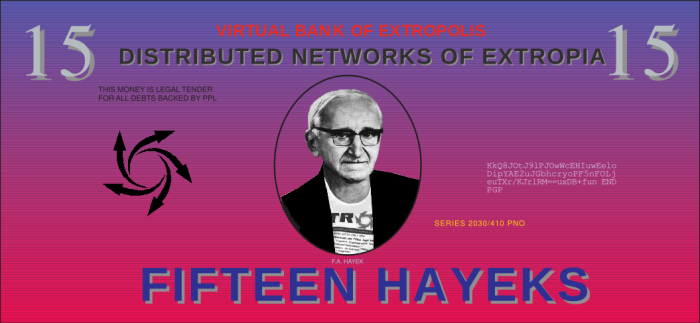
\includegraphics[scale=0.8]{img/fifteen-hayeks-note-extropy-15.png}
  \caption{Le billet fictif de 15 hayeks en couverture du magazine Extropy.}
\end{figure}

La monnaie numérique constituait donc l'un des sujets mis en avant par les extropiens. Mais ces derniers ne le faisaient pas autant que les cypherpunks qui, des années plus tard, tenteraient de mettre en pratique leur connaissance de la cryptographie pour en créer une.

\section*{Les cypherpunks}
\addcontentsline{toc}{section}{Les cypherpunks}

% Définition
Le mouvement cypherpunk est apparu en 1992 dans la Silicon Valley. Les cypherpunks étaient des gens qui prônaient l'utilisation proactive de la cryptographie en vue d'assurer la confidentialité et la liberté des individus dans le cyberespace. Ils s'opposaient à la surveillance, à la censure et à l'exploitation des données personnelles, et préconisaient la programmation et la publication ouverte de logiciels, préférablement sous licence libre, dans le but de les combattre.

% Terme cypherpunk
Le terme cypherpunk est un mot-valise composé des mots anglais \eng{cypher}, signifiant chiffre, dans le sens de code secret, et \eng{punk}, désignant originellement un voyou. Les cypherpunks étaient donc des rebelles amateurs de cryptographie. Le terme était directement calqué sur le mot cyberpunk, dont le préfixe cyber- fait référence à la cybernétique, la science des systèmes complexes et des réseaux, et pour cause~: le mouvement était partiellement issu du cyberpunk.

% Mouvement / genre cyberpunk
Le cyberpunk était un mouvement culturel construit autour de la littérature de science-fiction, qui s'inspirait à la fois de la sous-culture des punks et de la mouvance des hackers. Même si l'esthétique datait de la fin des années 70, le genre littéraire a largement été inauguré par l'écrivain William Gibson via la publication de ses premières nouvelles à partir de 1981 et surtout de son roman \emph{Neuromancien} en juillet 1984. Le mot a quant à lui a été inventé en 1983 par Bruce Bethke\sendnote{«~Comment ai-je créé ce mot~? De la même manière que n'importe quel nouveau mot, je suppose~: par la combinaison. J'ai pris une poignée de racines -- cyber, techno, etc. --, je les ai mélangées à un tas de termes désignant des jeunes socialement désorientés, et j'ai essayé les différentes combinaisons jusqu'à ce que l'une d'entre elles sonne tout simplement juste.~» -- Bruce Bethke, \eng{Cyberpunk: a short story by Bruce Bethke}, 1997~: \url{http://www.infinityplus.co.uk/stories/cpunk.htm}.} et popularisé par Gardner Dozois en décembre 1984 dans un éditorial pour le Washington Post\sendnote{Gardner Dozois, \eng{Science Fiction in the Eighties}, 30 décembre 1984~: \url{https://www.washingtonpost.com/archive/entertainment/books/1984/12/30/science-fiction-in-the-eighties/526c3a06-f123-4668-9127-33e33f57e313/}.}. % "How did I actually create the word? The way any new word comes into being, I guess: through synthesis. I took a handful of roots --cyber, techno, et al-- mixed them up with a bunch of terms for socially misdirected youth, and tried out the various combinations until one just plain sounded right."

% Combinaison de haute technologie et de bassesse humaine
La caractéristique principale du genre cyberpunk était de décrire un futur dystopique où la technique de pointe était omniprésente (implants informatiques, réalité augmentée, réalité virtuelle, intelligence artificielle, robots) et où la société était sujette à la consommation à outrance (drogue, sexe, etc.), au crime et à l'avarice de corporations. Le cyberpunk décrivait ainsi un monde combinant haute technologie et bassesse humaine, pour reprendre l'expression de Bruce Sterling\sendnote{Bruce Sterling, «~\eng{Preface}~», in \eng{Burning Chrome} (William Gibson), 1986.}, dont le héros tentait de s'extraire tant bien que mal. % "Gibson's classic one-two combination of lowlife and high-tech"

% Contreculture cyberdélique
De ce genre cyberpunk est né tout un mouvement d'individus qui partageaient la même vision du monde, formant notamment une contreculture cyberdélique, née de la fusion de cyberculture et du psychédélisme. Cette sous-culture en vogue dans la Silicon Valley était incarnée par la revue \eng{High Frontiers}, fondée en 1984 par R. U. Sirius, et qui est plus tard devenue \eng{Reality Hackers} puis \eng{Mondo 2000}.

% Différence avec les cypherpunks
Les cypherpunks étaient ainsi inspirés par ce mouvement. Toutefois, ils n'étaient pas pour autant des cyberpunks~: s'ils avaient bien conscience des scénarios dystopiques qui pouvaient dériver de l'évolution technique (notamment en ce qui concerne la surveillance), ils ne partageaient pas la même vision pessimiste relayée par le cyberpunk. De ce fait, le mouvement cypherpunk constituait en quelque sorte une réaction au cyberpunk, dans le sens où il postulait, à l'instar des extropiens, que l'évolution technique pouvait amener les êtres humains à s'émanciper plutôt qu'à tomber dans l'esclavage mutuel.

% True Names
Les cypherpunks basaient en particulier leurs réflexions sur une longue nouvelle publiée en 1980 par l'auteur de science-fiction Vernor Vinge, intitulée \eng{True Names}. Cette nouvelle, qui abordait des thèmes propres au genre cyberpunk sans en être strictement\sendnote{«~Je ne me considère certainement pas comme un écrivain cyberpunk. [...] Je pense que True Names partage un grand nombre d'idées techniques avec les récits cyberpunk. Je vois également deux différences substantielles entre True Names et les récits que l'on appelle généralement "cyberpunk". Premièrement, le cyberpunk montre davantage les aspects les plus sombres de la société future. Dans certains cas, il s'agit simplement d'un style dur à cuire. Dans d'autres cas, il capture la douleur d'un changement social très rapide. Deuxièmement, le cyberpunk est souvent pessimiste quant à la possibilité de changements sociaux et techniques, ce qui peut en fait être une très bonne chose.~» -- Vernor Vinge (interrogé par Michael Synergy), «~Hurtling Towards the Singularity~», \emph{Mondo 2000 issue 1}, 1989~: \url{https://archive.org/details/Mondo.2000.Issue.01.1989/page/n115/mode/2up}.}, contait l'histoire de Roger Pollack, un individu agissant au sein d'un groupe de pirates dans un monde virtuel appelé «~\eng{The Other Plane}~», qui utilisait le pseudonyme de Mr. Slippery et qui faisait attention à ne surtout pas révéler son «~Vrai Nom~» (à savoir son nom civil) au risque de subir une «~Vraie Mort~» (par exécution étatique). Cet enjeu correspondait ainsi à l'enjeu principal de la cryptographie~: la préservation de l'anonymat dans le but de conserver sa liberté et, \emph{in fine}, sa vie. % "I certainly don't think of myself as a cyberpunk writer. A couple of months ago, I was asked whether I thought True Names was cyberpunk. I wrote a note that appeared in Science Fiction Lovers. Let me just read that to you: "I think there's a large set of tech ideas that True Names shares with cyberpunk stories. I also see two substantial differences between True Names and the stories that are usually called 'cyberpunk.' One: cyberpunk shows more of future society's ugly underbelly. In some cases this is simply hardboiled style. In some cases, it captures the pain of very fast social change. Two: cyberpunk is often pessimistic about the possibility of social and technological change, which may in fact be a wonderfully good thing."

% Différence avec les extropiens
Les cypherpunks avaient ainsi le regard tourné vers l'avenir. Mais leur préoccupation concernaient surtout l'avenir proche~: c'était la confidentialité dans le cyberespace naissant\sendnote{Le terme «~cyberespace~» (\eng{cyberspace} en anglais) a été forgé par William Gibson dans sa nouvelle \emph{Gravé sur Chrome} publiée en juillet 1982, pour désigner la représentation virtuelle des flux de données sur Internet. Le terme «~matrice~» (\eng{matrix}) était utilisé en tant que synonyme.}. C'est pourquoi leur mouvement pouvait rassembler des optimistes et des pessimistes, des extropiens et des cyberpunks, qui trouvaient du sens dans cette lutte contre la surveillance de masse.

% Tim May
Le mouvement cypherpunk est initialement le fruit de la pensée et de l'action de Timothy C. May, dit «~Tim May~». Tim May était un scientifique, ingénieur et informaticien né en 1951 en périphérie de Washington D.C. Passionné de science-fiction et de physique, il avait travaillé pour Inter de 1974 où il avait contribué à résoudre le problème des particules alpha dans les circuits intégrés\sendnote{Timothy C. May, Murray H. Woods, \eng{Alpha-Particle-Induced Soft Errors in Dynamic Memories}, janvier 1979~: \url{https://gwern.net/doc/cs/hardware/1979-may.pdf}.}. Il avait accumulé une certaine fortune au cours de ces années, si bien qu'en 1986 (à l'âge de 35 ans), il décidait de prendre sa retraite pour se consacrer à ses passions politiques.

% Origine de l'idée cryptoanarchiste
Tim May a rencontré Phil Salin en 1987, par l'intermédiaire de Chip Morningstar\sendnote{Paralelní Polis, \eng{Timothy C. May - Thirty Years of Crypto Anarchy}, 11 février 2017~: \url{https://www.youtube.com/watch?v=TdmpAy1hI8g\&t=360s}.}. Il a ainsi pu discuter des implications de la cryptographie, avec Salin et sa femme, ainsi que d'autres personnes comme Marc Stiegler. C'est ce qui l'a poussé à écrire le \emph{Manifeste crypto anarchiste} en août 1988 qu'il a partagé avec Phil Salin et d'autres\sendnote{Timothy C. May, \eng{Cyphernomicon}, 16.3.4.}.

% Manifeste crypto anarchiste
Dans ce manifeste, il posait les bases de ce qui allait devenir la doctrine des cypherpunks et décrivait le potentiel d'émancipation individuelle apporté par la cryptographie et par l'anonymat. Le manifeste, pastiche ironique du \emph{Manifeste du parti communiste}, décrivait comment l'avènement des méthodes cryptographiques modernes allait, d'après lui, déstabiliser l'État en permettant aux individus d'échanger librement de l'information et de la richesse. En particulier, il écrivait~:

\begin{quote}
«~Tout comme la technique de l'imprimerie a altéré et réduit le pouvoir des corporations médiévales et la structure sociale de pouvoir, les méthodes cryptologiques altèrent fondamentalement la nature de l'interférence de l'État et des grandes entreprises dans les transactions économiques.\sendnote{Timothy C. May, \eng{The Crypto Anarchist Manifesto}, \wtime{22/11/1992 20:11:24 UTC}~: \url{https://cypherpunks.venona.com/date/1992/11/msg00204.html}.}~»
\end{quote} % "Just as the technology of printing altered and reduced the power of medieval guilds and the social power structure, so too will cryptologic methods fundamentally alter the nature of corporations and of government interference in economic transactions."

% Eric Hughes
Mais Tim May n'était pas seul à penser de cette manière et communiquait avec d'autres personnes qui partageaient ses idées. C'était le cas de son ami Eric Hughes, un jeune mathématicien et programmeur qui avait grandi dans une famille mormone en Virginie près de Washington et à Salt Lake City. Ce dernier avait travaillé brièvement pour DigiCash à Amsterdam avant de revenir sur la côte Ouest\sendnote{Timothy C. May, \eng{Hackers Conference Report}, \wtime{11/11/1992 08:55:26 UTC}~: \url{https://cypherpunks.venona.com/date/1992/11/msg00019.html}.}. En mai 1992, alors qu'il cherchait à emménager dans la Silicon Valley, lui et Tim May avaient longuement discuté de cryptographie, à tel point qu'ils ont décidé de reproduire ce type d'échange avec un plus grand nombre de personnes en organisant des réunions physiques. % Mormonisme d'Eric Hughes : cf. Crypto (Steven Levy), p. 259

% Première réunion
La première réunion du mouvement cypherpunk a eu lieu au cours de la journée du 19 septembre 1992, dans la maison d'Eric Hughes à Oakland. L'accès à cette réunion se faisait uniquement sur invitation afin de préserver la discrétion du mouvement. Libertariens pour la plupart, extropiens pour certains, les invités étaient des connaissances de May et Hughes issues de la communauté des hackers et des entreprises informatiques de la région. Durant la réunion, Tim May y a lu le \emph{Manifeste crypto anarchiste}. Une animation sous la forme d'un «~jeu de la crypto anarchie~» a eu lieu~: ce jeu consistait à simuler un réseau de mélange par l'échange et l'ouverture d'enveloppes de papier.\sendnote{Certains détails de la formation des cypherpunks sont issus de l'ouvrage \eng{Crypto: How the Code Rebels Beat the Government--Saving Privacy in the Digital Age} (pp. 257 -- 266) de Steven Levy publié en 2001.}

% John Gilmore, né en 1955
Parmi les invités se trouvait John Gilmore, un informaticien américain qui avait été l'un des premiers employés de Sun Microsystems. Il avait co-créé la hiérarchie ouverte alt.* sur Usenet et il était un contributeur majeur du projet GNU. Alors en retraite anticipé depuis 1986, tout comme May, il s'était engagé dans l'activisme dans le but de protéger les libertés civiles sur Internet. En 1989, il était le co-fondateur de Cygnus Support, une entreprise spécialisée dans le support professionnel de composants fondés sur GNU. Il a également co-fondé l'\eng{Electronic Frontier Foundation} (EFF) en 1990 aux côtés de Mitch Kapor et de John Perry Barlow, qui était une ONG internationale de protection des libertés sur Internet. Lui aussi voyait la cryptographie comme une moyen de libération individuelle\sendnote{«~Et si nous pouvions construire une société dans laquelle les informations ne seraient jamais collectées~? [...] C'est le genre de société que je veux construire.  Je veux que soit garantie - par la physique et la mathématique, pas par des lois - la possibilité de bénéficier de choses telles qu'une véritable confidentialité des communications personnelles, [...] une véritable confidentialité des enregistrements personnels, [...] une véritable liberté de commerce, [...] une véritable confidentialité financière [et] une véritable contrôle de l'identification.~» -- John Gilmore, \eng{Privacy, Technology, and the Open Society}, 28 mars 1991~: \url{http://www.toad.com/gnu/cfp.talk.txt}~; archive~: \url{https://web.archive.org/web/19991003163945/http://www.toad.com/gnu/cfp.talk.txt}.}. % "What if we could build a society where the information was never collected?  Where you could pay to rent a video without leaving a credit card number or a bank number?  Where you could prove you're certified to drive without ever giving your name?  Where you could send and receive messages without revealing your physical location, like an electronic post office box? That's the kind of society I want to build.  I want a guarantee -- with physics and mathematics, not with laws -- that we can give ourselves things like real privacy of personal communications, (...) real privacy of personal records, (...) real freedom of trade, (...) real financial privacy, (...) real control of identification." %

% Judith Milhon
Une autre personne présente durant cette réunion fondatrice était l'activiste Judith Milhon, une femme née en 1939 qui avait participé au mouvement des droits civiques pour l'abolition des discriminations raciales dans les années 60 et avait été emprisonnée pour désobéissance civile\sendnote{Sean Dodson, \eng{Judith Milhon: making the Internet a feminist issue}, 8 août 2003~: \url{https://www.theguardian.com/technology/2003/aug/08/guardianobituaries.obituaries}.}. Programmeuse, hackeuse, elle était alors la co-éditrice de la revue cyberpunk \eng{Mondo 2000}, à laquelle elle participait sous le nom de plume de St. Jude. Elle était également la compagne d'Eric Hughes, malgré leur grande différence d'âge.

% Terme cypherpunk
C'est elle qui a donné leur nom aux cypherpunks lors de cette réunion, sur le ton de la plaisanterie. «~Je pense que vous êtes des cryptoanarchistes -- ce que j'appellerais des cypherpunks~!~», a-t-elle écrit par la suite\sendnote{Judith Milhon, \eng{secretions}, \wtime{25/09/1992 10:01:26 UTC}~: \url{https://cypherpunks.venona.com/date/1992/09/msg00013.html}.}. Le terme capturait bien l'esprit de la cryptoanarchie, tout en donnant au mouvement un côté moins formel et dogmatique. En particulier, les gens préoccupés par ces enjeux n'étaient pas tous anarchistes~: ils pouvaient s'opposer fermement à l'autoritarisme et à la surveillance, sans pour autant vouloir remettre en cause les fondements même de l'État\sendnote{«~De plus, cela donne à tort l'impression que "cypherpunk" est synonyme d'"anarchiste". Il se trouve que je suis anarchiste, mais ce n'est pas ce en quoi croient la plupart des personnes associées au terme "cypherpunk", et il n'est pas juste de les dépeindre ainsi - bon sang, de nombreuses personnes sur cette liste de diffusion sont ouvertement hostiles à l'anarchisme. Je ne veux pas que les gens pensent qu'il faut détester l'idée même d'État pour aimer la cryptographie.~» -- Perry E. Metzger, \eng{Re: PC Expo summary!!}, \wtime{01/07/1994 12:13:09 UTC}~: \url{https://cypherpunks.venona.com/date/1994/07/msg00014.html}.}. C'est ce côté indéfini et décontracté qui a fait que le terme a été adopté immédiatement. % "Also, it unfairly makes it look like "cypherpunk" means "anarchist". Now, it happpens that I am an anarchist, but that isn't what most people associated with the term "cypherpunk" believe in, and it isn't fair to paint them that way -- hell, many people on this mailing list are overtly hostile to anarchism. I don't want people to think you have to hate the idea of government in order to like cryptography."

% Création de la mailing list
Après la réunion, Eric Hughes, avec l'aide de Hugh Daniel, a créé une liste de diffusion de courrier électronique nommée «~Cypherpunks~». Le courriel de bienvenue\sendnote{Eric Hughes, \eng{No Subject}, \wtime{22 Sep 92 05:43:46 UTC}~: \url{https://cypherpunks.venona.com/date/1992/09/msg00001.html}.} a été envoyé dans la soirée du 21 septembre (PDT). La liste était relayée par le serveur associé au nom de domaine \texttt{toad.com} appartenant à John Gilmore. Ce dernier a aussi offert la disponibilité des locaux de Cygnus pour les réunions ultérieures.

% Succès de la liste
La liste a accueilli de nombreuses discussions relatives à la cryptographie et à son utilisation concrète, dont notamment l'argent liquide électronique. Beaucoup de gens sont intervenus dès les premiers mois, comme par exemple l'ancien pirate téléphonique John Draper. En un an à peine, la liste recensait ainsi plus de 500 participants. % Source : Cyphernomicon 3.3.14

% Hal Finney
L'un de ces participants était Harold T. Finney \textsc{ii}, dit «~Hal Finney~», informaticien et cryptographe américain, diplômé de Caltech et programmeur de jeux vidéos pour les consoles Intellivision et Atari VCS. Extropien et enthousiasmé la popularisation d'Internet, il était obsédé par la cryptographie, à tel point qu'il était rentré en contact avec Phil Zimmermann pour travailler avec lui sur la version 2.0 de PGP, qui était sortie le 2 septembre 1992. Hal Finney était aussi fasciné par les idées de David Chaum. En novembre 1992, il écrivait à la liste de diffusion~:

\begin{quote}
«~Nous voici confrontés aux problèmes de la perte de confidentialité, de l'informatique trompeuse, des bases de données massives, de l'augmentation de la centralisation -- et Chaum propose une direction à suivre complètement différente, une direction qui met le pouvoir entre les mains des individus plutôt que celles des États et des grandes entreprises. L'ordinateur peut être utilisé comme un outil pour libérer et protéger les personnes, plutôt que pour les contrôler.\sendnote{Hal Finney, \eng{Why remailers...}, \wtime{16/11/1992 01:30:02 UTC}~: \url{https://cypherpunks.venona.com/date/1992/11/msg00108.html}.}~»
\end{quote}

% Appel à la pratique
La vision des cypherpunks était claire~: mettre en pratique ce qui avait été jusque-là de vagues spéculations. Il était en effet stérile de théoriser des choses si cela ne se traduisait pas par des actions concrètes. Cet esprit pratique a été parfaitement résumé par Eric Hughes dans son \emph{Manifeste d'un Cypherpunk} envoyé à la liste de diffusion en mars 1993, où il écrivait alors~:

\begin{quote}
«~Nous devons défendre notre propre vie privée si nous voulons en avoir une. Nous devons nous rassembler et créer des systèmes qui rendent possibles les transactions anonymes. Depuis des siècles, les gens défendent leur vie privée par des chuchotements, par l'obscurité, par des enveloppes, des portes fermées, des poignées de main secrètes et des messagers. Les techniques du passé ne permettaient pas une forte confidentialité, mais les techniques électroniques le permettent.

Nous, les Cypherpunks, nous consacrons à construire des systèmes anonymes. Nous défendons notre confidentialité avec la cryptographie, avec les systèmes anonymes de transfert de courriels, avec les signatures numériques, et avec la monnaie électronique.

Les Cypherpunks écrivent du code. Nous savons que quelqu'un doit écrire un logiciel pour défendre la vie privée, et puisque nous ne pouvons pas avoir de vie privée si nous ne le faisons pas tous, nous allons l'écrire. Nous publions notre code pour que nos collègues Cypherpunks puissent le mettre en pratique et expérimenter avec. Notre code est libre d'utilisation pour tous, dans le monde entier. Nous ne nous soucions guère que vous n'approuviez pas les logiciels que nous écrivons. Nous savons que les logiciels ne peuvent pas être détruits et qu'un système largement dispersé ne peut pas être arrêté.\sendnote{Eric Hughes, \eng{RANTS: A Cypherpunk's Manifesto}, \wtime{17/03/1993 19:51:06 UTC}~: \url{https://cypherpunks.venona.com/date/1993/03/msg00392.html}.}~»
\end{quote} % "We must defend our own privacy if we expect to have any.  We must come together and create systems which allow anonymous transactions to take place.  People have been defending their own privacy for centuries with whispers, darkness, envelopes, closed doors, secret handshakes, and couriers.  The technologies of the past did not allow for strong privacy, but electronic technologies do.
%
% We the Cypherpunks are dedicated to building anonymous systems.  We are defending our privacy with cryptography, with anonymous mail forwarding systems, with digital signatures, and with electronic money.
%
% Cypherpunks write code.  We know that someone has to write software to defend privacy, and since we can't get privacy unless we all do, we're going to write it. We publish our code so that our fellow Cypherpunks may practice and play with it. Our code is free for all to use, worldwide.  We don't much care if you don't approve of the software we write.  We know that software can't be destroyed and that a widely dispersed system can't be shut down."

% Publicité
Deux mois plus tard, en mai 93, le mouvement était définitivement lancé~: les cypherpunks faisaient la une du magazine Wired, récemment fondé dans le but de parler de l'incidence culturelle, économique et politique des techniques émergentes. Tim May, Eric Hughes et John Gilmore apparaissaient masqués sur la couverture, et un long article détaillait leurs idées et leurs revendications\sendnote{Steven Levy, \eng{Crypto Rebels}, 1\ier{} février 1993~: \url{https://www.wired.com/1993/02/crypto-rebels/}~; archive~: \url{https://web.archive.org/web/20151102012232/https://www.wired.com/1993/02/crypto-rebels/}.}. Les cypherpunks ont également été présentés par la suite dans les revues \eng{Whole Earth Review} et \eng{The Village Voice}\sendnote{\eng{Cypherpunks, e-Money and the Technologies of Disconnection}~: \url{https://archive.org/details/sim_whole-earth_summer-1993_79/page/40/mode/2up}~; \url{http://www.juliandibbell.com/texts/codewars.html}.}.

\section*{Les accomplissements des cypherpunks}
\addcontentsline{toc}{section}{Les accomplissements des cypherpunks}

Le mouvement cypherpunk est né juste après le triomphe des États-Unis dans la guerre froide les opposant à l'URSS et au début de la démocratisation d'Internet, amorcée notamment par la popularisation de Usenet et par l'apparition du World Wide Web. Il est apparu en quelque sorte au bon moment pour alerter et accompagner ce qui allait suivre.

% --- Guerre contre la cryptographie ---

\textbf{Guerre contre la cryptographie.} Le premier accomplissement des cypherpunks a été leur rôle dans la guerre contre la cryptographie, orchestrée par l'État fédéral étasunien.

La première réaction étatique a été la guerre contre PGP. La version 1.0 de PGP avait été publiée sur Internet en juin 1991 et la version 2.0 en septembre 1992, en dehors des États-Unis. En 1993, le logiciel de chiffrement commençait à se populariser.

Lorsque Phil Zimmermann a publié la version 1.0 de PGP par le biais de \eng{bulletin board systems} et de Usenet en juin 1991, il savait qu'il risquait d'attiser une réponse du pouvoir. La Réglementation américaine sur le trafic d'armes au niveau international (\eng{International Traffic in Arms Regulations} en anglais ou ITAR) considérait en effet les produits cryptographiques comme des «~munitions~» et en interdisait l'exportation sans licence. Par conséquent, une enquête contre Zimmermann a été ouverte par l'État fédéral en février 1993.

% Réaction
Cette décision a naturellement provoqué une forte résistance de la part des cypherpunks qui, en réponse à cette loi absurde, se sont mis à partager le code de chiffrement dans une démarche de désobéissance civile. Le jeune britannique Adam Back l'a fait imprimer sur des t-shirts qu'il distribuait aux autres et certains ont été jusqu'à se le tatouer sur leur corps\sendnote{\url{http://www.cypherspace.org/adam/rsa/}}. En 1995, Phil Zimmermann a publié la version 2.6.2 de PGP dans un livre\sendnote{Philip Zimmermann, \eng{PGP: Source Code and Internals}, 1995~: \url{https://philzimmermann.com/EN/essays/BookPreface.html}.}, dans le but de réduire au maximum la distinction entre le code et l'expression, cette dernière étant protégée par le premier amendement de la Constitution des États-Unis. Il a bénéficié au passage du soutien du MIT\sendnote{Steven Levy, \eng{Cypher Wars}, 1994~: \url{https://www.wired.com/1994/11/cypher-wars/}~; archive~: \url{https://web.archive.org/web/20160403024823/https://www.wired.com/1994/11/cypher-wars/}.}.

Les charges contre Zimmermann ont finalement été abandonnées en 1996, lui permettant de créer son entreprise pour travailler sur PGP et d'engager des employés, comme Hal Finney. En novembre de la même année, Bill Clinton signait l'Ordre exécutif 13026 qui assouplissait considérablement les restrictions sur l'exportation des produits cryptographiques.

\textbf{Clipper.} Cependant, la guerre contre la cryptographie ne s'arrêtait pas là. Elle ne concernait en effet pas que les interdictions, mais aussi les obligations. Le projet de loi sénatoriale 266, proposé par Joe Biden en 1991, devait ainsi imposer l'existence d'une porte dérobée dans tous les appareils de communication~: % Joe Biden's S.266

\begin{quote}
«~Le Congrès estime que les fournisseurs de services de communications électroniques et les fabricants d'équipements de services de communications électroniques doivent veiller à ce que les systèmes de communications permettent au gouvernement d'obtenir le contenu en texte clair des communications vocales, de données et autres lorsque la loi l'autorise de manière appropriée.\sendnote{\eng{Comprehensive Counter-Terrorism Act of 1991}, 24 janvier 1991~: \url{https://www.congress.gov/bill/102nd-congress/senate-bill/266/text}.}~»
\end{quote} % "It is the sense of Congress that providers of electronic communications services and manufacturers of electronic communications service equipment shall ensure that communications systems permit the government to obtain the plain text contents of voice, data, and other communications when appropriately authorized by law."

% Puce Clipper
Ce projet s'est matérialisé le 16 avril 1993 par l'annonce par la Maison-Blanche de la puce Clipper, un cryptoprocesseur servant à chiffrer les messages vocaux et les données, qui implémentait (au travers de son algorithme Skipjack) un dispositif d'autorité de séquestre permettant aux agences étasuniennes de déchiffrer les communications au besoin. Cette puce était développée et produite par la NSA et était destinée à équiper les appareils électroniques vendus au grand public. La Maison-Blanche se justifiait en prétendant que la puce pourrait «~à la fois fournir aux citoyens respectueux de la loi un accès au chiffrement dont ils ont besoin et empêcher les criminels de l'utiliser pour cacher leurs activités illégales\sendnote{The White House, \eng{White House Annoucement of the Clipper Initiative}, 16 avril 1993~: \url{https://groups.csail.mit.edu/mac/classes/6.805/articles/crypto/clipper-announcement.html}.}~».

% Lutte contre Clipper
Cette annonce n'a pas manqué de faire réagir les cypherpunks qui se sont opposés en bloc à ce projet orwellien. Cependant, la lutte n'a pas été longue~: en juin 1994, le cypherpunk Matt Blaze a découvert une vulnérabilité au sein du dispositif d'autorité de séquestre\sendnote{John Markoff, \eng{At AT\&T, No Joy on Clipper Flaw}, 3 juin 1994~: \url{https://www.nytimes.com/1994/06/03/business/at-at-t-no-joy-on-clipper-flaw.html}~; Matt Blaze, \eng{Paper available via ftp}, \wtime{05/06/1994 00:01:57 UTC}~: \url{https://cypherpunks.venona.com/date/1994/06/msg00319.html}.}, qui rendait le dispositif inefficace et permettait à la puce d'être utilisée pour chiffrer les données normalement. À partir de là, le projet a perdu progressivement en ampleur pour être définitivement abandonné en 1996\sendnote{Cette victoire n'a cependant pas empêché pas les agences étasuniennes d'espionner leur propre population de manière massive, comme l'ont montré les révélations d'Edward Snowden en 2013. -- Voir Glenn Greenwald, \eng{NSA collecting phone records of millions of Verizon customers daily}, 6 juin 2013~: \url{https://www.theguardian.com/world/2013/jun/06/nsa-phone-records-verizon-court-order}.}. Le cyberespace était déclaré indépendant\sendnote{John Perry Barlow, \eng{A Declaration of the Independence of Cyberspace}, 8 février 1996~: \url{https://www.eff.org/fr/cyberspace-independence}.}.

% --- Autres accomplissements ---

Comme on l'a observé, l'optique des cypherpunks était d'être dans l'action, d'écrire du code et de partager du code qui puisse être utilisé. Ils se sont donc focalisés sur la construction de systèmes axés sur trois aspects majeurs~: la protection de la vie privée, la diffusion de l'information et le commerce en ligne. % combinaison de techniques cryptographiques permettant d'assurer la confidentialité, l'authenticité et l'intégrité des données. Réputation.

% Serveurs de courriel anonymes (remailers)
Le premier domaine d'innovation a été celui des serveurs de courriel anonyme, qui permettaient de retransmettre les courriers électroniques de façon à masquer l'identité de leur expéditeur. Le premier serveur de ce type a mis en place par Eric Hughes et Hal Finney pour la liste des cypherpunks dès octobre 1992, il utilisait PGP pour le chiffrement\sendnote{Hal Finney, \eng{New remailer...}, \wtime{13/10/1992 20:31:48 UTC}~: \url{https://cypherpunks.venona.com/date/1992/10/msg00082.html}.}. En 1994, Lance Cottrell a amélioré la chose en proposant Mixmaster\sendnote{Lance Cottrell, \eng{1st Draft Mixmaster chaining instructions}, \wtime{21/11/1994 01:07:02 UTC}~: \url{https://cypherpunks.venona.com/date/1994/11/msg00158.html}.}, qui permettait d'envoyer des courriels par paquets de taille fixe et de les réordonner, pour empêcher le traçage des courriels par la surveillance de l'activité du serveur. % Cypherpunks remailer: type I (1992); Mixmaster remailer: type II (1994); Mixminion remailer: type III (2002)

% Navigation
Outre le courriel, l'objectif des cypherpunks était de rendre la navigation sur Internet plus anonyme. L'émergence du Web était jugée trop transparente.

% Réseau Freedom
C'était l'idée des frères Austin et Hamnett Hill qui ont lancé le réseau Freedom en 1999 par l'intermédiaire de leur entreprise Zero-Knowledge Systems, qui employait notamment les cypherpunks Ian Goldberg et Adam Back\sendnote{Chris Oakes, \eng{Zero-Knowledge: Nothing Personal}, 9 février 1999~: \url{https://www.wired.com/1999/02/zero-knowledge-nothing-personal/}.}. Mais cette expérience s'est arrêtée en 2001, faute d'utilisation suffisante.

% Tor
Un autre projet dans lequel les cypherpunks se sont impliqués est le réseau Tor, qui fonctionne comme on l'a déjà expliqué grâce au routage en ognon, d'où son nom (Tor est l'acronyme de \eng{The Onion Router}. En effet, si Tor est le résultat d'une recherche militaire provenant de la Navy, les individus qui ont travaillé sur son implémentation n'en avaient pas moins des convictions allant dans le sens des cypherpunks. Roger Dingledine et Nick Mathewson, les deux informaticiens qui ont aidé Paul Syverson dans cette conceptions, en faisaient partie~: le premier était derrière le projet Free Haven, qui avait pour but de développer un système décentralisé de stockage de données\sendnote{\url{https://www.freehaven.net/}}~; le second est crédité pour avoir créé le programme de serveur de courriel anonyme Mixminion\sendnote{George Danezis, Roger Dingledine, Nick Mathewson, \eng{Mixminion: Design of a Type III Anonymous Remailer Protocol}, 2003~: \url{https://git.gnunet.org/bibliography.git/plain/docs/minion-design.pdf}.}. On peut également citer le jeune Jacob Appelbaum, qui s'est fortement impliqué dans le projet Tor entre 2004 et 2016.

% BlackNet
Un troisième accomplissement a été la fluidification des flux informationnels, notamment face à la censure. En 1993, Tim May a repris le modèle de l'AMIX de Phil Salin pour introduire un concept de place de marché de l'information appelé BlackNet. Cette plateforme devait servir à échanger des secrets commerciaux, des recettes de fabrication, des techniques relatives aux nanotechnologies, des informations sur les décisions d'entreprises, au moyen de «~CryptoCredits~», la monnaie interne du système. Il s'agissait donc de libérer l'information des contraintes étatiques~: «~BlackNet est officiellement non idéologique, mais considère les États-nations, les lois d'exportation, les lois sur les brevets, les considérations de sécurité nationale, etc. comme des reliques de l'ère pré-cyberspatiale~», écrivait Tim May\sendnote{Timothy C. May, \eng{no subject (file transmission)}, 17 août 1993, \url{https://cypherpunks.venona.com/date/1993/08/msg00538.html}.}.

% Autres, Cryptome
Le concept de BlackNet était une simple expérience de pensée et n'a jamais été mis en œuvre. Toutefois, il a préfiguré d'autres modèles qui ont ouvert la voie au partage d'informations sensibles sur Internet. C'était par exemple le cas de Cryptome, un site web lancé en 1996 par le cypherpunk John Young pour héberger des documents sensibles et censurés par les États\sendnote{\eng{Cryptome JYA Archive}~: \url{https://cryptome.org/jya/}.}.

% WikiLeaks
Mais c'était surtout le cas de WikiLeaks, la plateforme facilitant la publication de documents classifiés fondée en 2006 par l'informaticien australien Julian Assange. Julian Assange était un cypherpunk assumé~: il envoyait des courriels sur la liste depuis au moins 1995 et a par la suite co-écrit un livre à ce sujet\sendnote{Julian Assange, Jacob Appelbaum, Andy Müller-Maguhn, Jérémie Zimmermann, \eng{Cypherpunks: Freedom and the Future of the Internet}, 2012.}. WikiLeaks a permis le développement de l'activité des lanceurs d'alertes ou des \eng{whistleblowers} qui révèlent les agissements illégaux ou injustes de leurs employeurs, et en particulier des États, largement inaugurée par la publication des Pentagon Papers en 1971 par Daniel Ellsberg. Grâce à l'utilisation du chiffrement et de Tor, WikiLeaks permettait aux personnes à l'origine des fuites de conserver leur anonymat.

% Mojo Nation
Enfin, sur un autre plan, les cypherpunks se sont également investis dans le développement du pair-à-pair. En 2000, le développeur Jim McCoy, cypherpunk de la première heure, a ainsi lancé Mojo Nation, un projet de plateforme d'échange de fichiers en pair-à-pair intégrant une devise interne\sendnote{Damien Cave, \eng{The Mojo solution}, 9 octobre 2000~: \url{https://www.salon.com/2000/10/09/mojo_nation/}.}. En 2001, Bram Cohen, qui travaillait avec lui a quitté le projet et lancé BitTorrent, qui est devenu la référence pour le partage de fichiers au cours des années. Mojo Nation, alors renommé en Mnet, a été repris par Zooko Wilcox, qui a lancé son propre système en 2006 sous le nom de Tahoe-LAFS (et qui a ensuite contribué à lancer ZCash en 2016). % TAZ "temporary autonomous zone" Hakim Bey, 1991

% Cybermonnaie
Mais ce qu'il manquait à tous ces systèmes, c'était une monnaie numérique robuste qui soit adaptée au cyberespace, chose à laquelle les cypherpunks aspiraient depuis le début. Leurs modèles possédaient parfois des unités de compte internes, mais elles étaient très instables. Malheureusement, une telle monnaie ne serait conçue que des années plus tard, en 2008, au travers de Bitcoin.

% Silk Road : BlackNet précédait aussi aussi en quelque sorte la place de marché Silk Road, créée par Ross Ulbricht en 2011, qui a été essentiellement utilisée pour la vente de drogues diverses.
% Le tristement célèbre concept d'Assassination Politics\sendnote{\url{https://cryptome.org/ap.htm}~; mentionné sur cypherpunks en déc. 1995~: \url{https://cypherpunks.venona.com/date/1995/12/msg00570.html}, \url{https://cypherpunks.venona.com/date/1995/12/msg00928.html}}.

\section*{Une guerre perpétuelle}
\addcontentsline{toc}{section}{Une guerre perpétuelle}

Bitcoin s'inscrit pleinement dans la guerre technologique opposant l'autorité à la liberté. Son code n'est pas neutre~: il n'est pas une vague technique qu'on puisse utiliser dans un sens ou dans l'autre, mais il a pour objectif clair d'amener plus de liberté individuelle.

Bitcoin est issu d'idéologies qui appellent à la pratique~: les libristes appelaient à la publication sous licence libre dans le but de mettre en commun l'ensemble des connaissances de l'humanité, les extropiens appelaient à la recherche et à l'expérimentation pour améliorer drastiquement les conditions de vie matérielles de l'être humain, les cypherpunks appelaient à écrire du code afin de préserver la confidentialité des individus dans le cyberespace.

Satoshi Nakamoto était-il un cypherpunk~? Sans en faire pleinement partie et sans s'en réclamer, le créateur de Bitcoin était clairement influencé par l'héritage cypherpunk. D'abord, il a utilisé un pseudonyme et, par de bonnes pratiques, comme l'utilisation de PGP, de Tor et de Namecheap, il est parvenu à préserver son anonymat malgré presque trois années d'activité en ligne. Puis, il a publié le livre blanc sur la liste de diffusion dédiée à la cryptographie gérée par Perry Metzger, qui était la digne héritière de la liste cypherpunk, qui avait malheureusement périclité à la fin des années 90. Ensuite, il semblait démontrer une bonne connaissance de ce qui s'était passé et de ce qui avait été fait avant lui, malgré quelques lacunes. Enfin, il a programmé un outil pour arriver à un résultat émancipateur. Il semble donc raisonnable d'assimiler Satoshi aux cypherpunks tout en gardant en tête qu'il a toujours été mesuré dans ses quelques jugements politiques.

% Clé PGP de Satoshi : \sendnote{\url{https://bitcointalk.org/index.php?topic=458.msg5772\#msg5772}}

\printendnotes
% Copyright (c) 2022 Ludovic Lars
% This work is licensed under the CC BY-NC-SA 4.0 International License

\chapter{La cybermonnaie avant Nakamoto}
\label{ch:cybermonnaie}

La cybermonnaie est une monnaie dont le fonctionnement repose entièrement sur un réseau informatique appartenant à Internet. Elle est définie par ce réseau et elle est transférée par son intermédiaire. Plus spécifiquement, il s'agit d'une monnaie native du cyberespace, le nouvel espace créé par l'émergence d'Internet, conçu comme une juridiction séparée du monde physique.

Une forme plus précise de cybermonnaie est l'idée d'argent liquide numérique, ou \eng{digital cash} en anglais, qui transcrit les propriétés des espèces sonnantes et trébuchantes dans le cyberespace. Toutefois, bien que cette idée date de l'émergence même d'Internet, elle n'a pas tout de suite pu être réalisée en raison de limitations techniques et conceptuelles. L'argent liquide numérique a fait l'objet d'une véritable quête, à laquelle ont participé de nombreux individus désireux d'utiliser Internet pour créer un nouveau paradigme économique, dont les cypherpunks.

Bitcoin est le résultat de cette quête. Il n'est ainsi pas sorti de nulle part~: il est le résultat de réflexions, de recherches et d'expérimentations dans le domaine de la cybermonnaie.

\section*{L'échange monétaire sur Internet}
\addcontentsline{toc}{section}{L'échange monétaire sur Internet}

% Échange informtationnel -> échange monétaire
Internet a généralisé le partage informationnel et, ce faisant, a créé un nouvel espace d'interactions humaines~: le cyberespace. L'apparition de cet espace a naturellement mené à l'émergence d'une demande pour l'échange monétaire, demande qui s'est manifestée au travers du développement du commerce électronique dans les années 90. Comme le résumait très bien Robert Hettinga en 1998, la problématique était la suivante~:

\begin{quote}
«~Depuis l'invention du télégraphe, le règlement des transactions financières se heurte à un problème~: comment faire des affaires à distance alors que le moyen le plus simple d'exécuter, de compenser et de régler une transaction est l'échange de certificats au porteur~?\sendnote{Robert A. Hettinga, \eng{Digital Bearer Settlement}, avril 1998~: \url{http://www.systemics.com/legal/digigold/discovery/postings/Geoecon.pdf}~; alt.~: \url{https://nakamotoinstitute.org/the-geodesic-market/\#digital-bearer-settlement}.}~»
\end{quote} % "Notre système actuel de règlement des transactions par "écriture comptable" a été inventé pour résoudre les problèmes posés par l'exécution des transactions à distance et la nécessité subséquente d'échanger physiquement des certificats au porteur pour le règlement. Nous avons aujourd'hui les moyens de revenir à un règlement au porteur 'encodé numériquement' tout en réduisant les coûts de trois ordres de grandeur." -- "Since the invention of the telegraph, financial transaction settlement has had a problem: how do you transact business at a distance when the simplest way to execute, clear and settle a transaction is with an exchange of bearer certificates? Our current system of so-called ‘book-entry' transaction settlement was invented in order to handle the problems caused by remote transaction execution and the subsequent need to physically exchange bearer certificates for settlement. We now have the means to return to ‘digitally encoded' bearer settlement with a three orders of magnitude cost saving."

% --- Première solution : crédit bancaire réglementé ---

La première solution était d'utiliser du crédit bancaire. L'usage de celui-ci comme intermédiaire d'échange s'était progressivement généralisé en Occident avec la bancarisation de la société. Au cours du temps, une solution technique avait prévalu~: la carte de paiement, aussi appelée carte de débit ou carte de crédit selon son fonctionnement. Cette solution n'était pas quelque chose de nouveau\sendnote{Le terme «~\eng{credit card}~» avait été utilisé en 1888 par Edward Bellamy, écrivain et journaliste socialiste américain et précurseur du mouvement technocratique, dans son roman de fiction spéculative \emph{Looking Backward}, pour désigner la carte de paiement des citoyens de sa supposée utopie. Ce type de carte s'était ensuite développé dans les années 1920-1930 aux États-Unis au travers de cartes délivrées indépendemment par Western Union, par les grands magasins, par les companies pétrolières et compagnies aériennes.}, mais s'était considérablement popularisée à partir des années 60, au travers de leur adoption par les banques et de la formation de sociétés spécialisées dans le transfert électronique de fonds comme NBI~/~Visa et Interbank~/~MasterCard\sendnote{Sur les origines du réseau Visa, voir David L. Stearns, \eng{Electronic Value Exchange: Origins of the VISA Electronic Payment System}, 2011. Le titre du livre est une référence au projet ambitieux de Dee Hock (le fondateur de Visa) de créer un protocole d'échange de valeur électronique (EVE) permettant d'effectuer l'intégralité des transactions sous forme électronique, ce qui donnerait lieu à «~la genèse d'une nouvelle forme de monnaie mondiale~». (Dee Hock, \eng{One From Many: VISA and the Rise of Chaordic Organization}, 2005, p.96)}.

% Edward Bellamy, \eng{Looking Backward: 2000–1887}, 1888.
% (BankAmericard) 1958 : Bank of America credit card program ; 1966 : BankAmericard Service Corporation (BASC) ; 1970 : National BankAmericard Incorporated (NBI) ; 1976 : Visa
% (Master Charge) 1966 : Interbank Card Association ; 1969 : Interbank rachète les droits (nom et marque) pour la carte Master Charge ; 1969 : MasterCard International ; 2002 : fusion avec Europay International ; 2006 : MasterCard Inc.
% Dee Hock, Electronic Value Exchange (EVE), 1975 : vision pour le futur de Visa et de la monnaie (toutes les transactions effectuées sous forme électronique)

% Paiements sur Internet
Mais le paiement par carte bancaire n'était pas forcément adapté au cyberespace, car difficile à mettre en place, coûteux et peu sécurisé à l'époque. C'est pourquoi, au milieu des années 90, on a vu émerger différentes solutions techniques permettant de faire des paiements sur Internet comme CyberCash\sendnote{Peter Wayner, \eng{Cybercash's Lesson in Web Survival}, 10 août 1998~: \url{https://www.nytimes.com/1998/08/10/business/cybercash-s-lesson-in-web-survival.html}~; archive~: \url{https://web.archive.org/web/20150527080844/https://www.nytimes.com/1998/08/10/business/cybercash-s-lesson-in-web-survival.html}.}, First Virtual\sendnote{\url{https://www.nytimes.com/1994/10/15/business/company-news-a-credit-card-for-on-line-sprees.html}} ou Open Market. Des systèmes de micropaiements ont également fait leur apparition à l'instar de CyberCoin (géré par CyberCash), NetBill\sendnote{Benjamin Cox, J. D. Tygar, Marvin Sirbu, \eng{NetBill Security and Transaction Protocol}, 1995~: \url{https://people.eecs.berkeley.edu/~tygar/papers/Netbill_securiy_and_transaction_protocol.pdf}.} et MilliCent\sendnote{Martín Abadi, Paul Gauthier, Steve Glassman, Mark S. Manasse, Patrick Sobalvarro, \eng{The Millicent Protocol for Electronic Commerce}, 1995~: \url{https://www.w3.org/Conferences/WWW4/Papers/246/}.}.

% CyberCoin : CyberCash Inc., NetBill : Carnegie Mellon University ; MilliCent : DEC Systems Research Center -> Compaq.
% CyberCash, 1994-2001 ; CyberCoin (système de micropaiements), 1996-1999 ; First Virtual, 1994-1998 ; MilliCent, 1995 -- 2001.
% NetCheque, Mondex, Gemplus

% PayPal
Ces systèmes ont fini par échouer, mais c'est dans cette niche que s'est développé le service PayPal à partir de 1999. Celui-ci était conçu pour être simple d'accès (PayPal signifie littéralement «~paie ton copain~»)~: il permettait des paiements faciles et sans frais, entre adresses de courrier électronique. Son modèle économique était de conserver les fonds des clients en banque et de percevoir les intérêts pour payer les coûts de fonctionnement et rémunérer les actionnaires. C'était donc un service de troisième couche, bâti au-dessus du système bancaire, lui-même basé sur le système de monnaie centrale.\sendnote{Sur l'histoire des débuts du service PayPal, voir Eric M. Jackson, \eng{The PayPal Wars: Battles With Ebay, the Media, the Mafia, and the Rest of Planet Earth}, 2012.}

% Surveillance et censure
En dépit des bonnes intentions de leurs créateurs, ces systèmes étaient complètement à la merci du régulateur. Ceux qui ont survécu se sont par conséquent engagés dans la surveillance et la censure, à un niveau jamais vu auparavant.

% Toutefois, toutes ces idées conduisaient à une monnaie numérique infiniment malléable, dont les transactions pouvaient être censurées et dont la masse monétaire pouvait être arbitrairement gonflée. Puisque ce type de monnaie reposait sur des tiers identifiés qui pouvaient observer l'intégralité des mouvement, il ne fallait pas espérer pouvoir échapper à long terme au contrôle. C'est ce que nous voyons avec la monnaie numérique de banque centrale, qui est la conséquence logique de la centralisation du crédit\sendnote{Voir chapitre~\ref{ch:adversaire}, section «~Les monnaies numériques de banque centrale~».}.

% --- Deuxième solution : monnaie numérique centralisée (mais rebelle) ---

La deuxième solution était d'émettre une nouvelle monnaie numérique, de manière centralisée, si besoin en l'adossant à une monnaie existante. Elle consistait à ne pas demander la permission, en jouant sur le flou juridique qui pouvait exister dans un domaine relativement nouveau.

% Jeux vidéo
Les jeux vidéos en ligne massivement multijoueurs, dont les fameux MMORPG, ont contribué à installer l'idée de monnaie numérique dans les esprits. On peut penser au Token, la monnaie native de Habitat, l'un des premiers MMORPG graphiques, développé en 1985 par Lucasfilm Games et jouable sur Commodore 64\sendnote{Chip Morningstar, F. Randall Farmer, \eng{The Lessons of Lucasfilm's Habitat}, mai 1990~: \url{http://www.fudco.com/chip/lessons.html}.}. On peut aussi citer les cas des pièces de métaux précieux dans Everquest en 1999, du dollar Linden de Second Life en 2003 ou encore de l'or de World of Warcraft en 2004. Tous ces exemples prouvaient qu'une économie réelle pouvait émerger d'une monnaie virtuelle\sendnote{Julian Dibbell, \eng{The Life of the Chinese Gold Farmer}, 17 juin 2007~: \url{https://www.nytimes.com/2007/06/17/magazine/17lootfarmers-t.html}.}.

% Hawthorne Exchange
Un exemple de ce type de système de monnaie numérique était le Hawthorne Exchange, lancé le 24 mars 1993 sur liste de diffusion extropienne par un individu du nom de Brian Holt Hawthorne\sendnote{Brian Holt Hawthorne, \eng{HEX: Introducing the Hawthorne Exchange}, \wtime{24/03/1993 06:20:21 UTC}~: \url{https://diyhpl.us/~bryan/irc/extropians/raided-mailing-list-archives/unzipped/disk-07/DIG30152}.}. Il s'agissait d'un marché de réputation pour les membres de la liste, dont l'unité de compte servant à l'échange était le Thorne. Le système était peu accessible et peu robuste, mais les extropiens l'ont utilisé et ont donné de la valeur au Thorne, par anticipation du futur. Quelques échanges monétaires contre du dollar et des services ont été réalisés entre les membres de la liste. Toutefois, le Hawthorne Exchange était simplement une expérimentation semi-ironique, le Thorne n'ayant aucun prétention à être une réelle monnaie, si bien que son auteur a décidé de l'arrêter en 1994.

% e-gold
Enfin, en 1996, est apparu le système e-gold, dont l'unité de compte était théoriquement adossée à de l'or. Le système reposait sur l'entreprise \eng{Gold \& Silver Reserve Inc.} fondée par Douglas Jackson, qui conservait l'or physique dans ses coffres. Il a connu un grand succès dans les années 2000 avant d'être fermé en 2007 par le Secret Service.

% Fermeture
Le problème avec ce type de monnaie, comme discuté dans le chapitre~\ref{ch:adversaire}, était qu'il dépendait toujours d'une entité qui constituait un point de défaillance unique. Ainsi, même si les personnes qui le géraient étaient bien intentionnées, et même s'il pouvait être utile dans certains cas, ce type de système n'était pas robuste et ne pouvait pas perdurer à long terme.

% --- Troisième solution : argent liquide électronique ---

La troisième solution était la conception d'un argent liquide électronique, confidentiel, non contrôlé et décentralisé. L'idée était de diminuer le rôle du tiers de confiance le plus possible pour que la monnaie en question se rapproche au mieux de l'argent liquide physique, de minimiser la confiance impliquée. Idéalement l'objectif était d'obtenir un «~or numérique~» qui soit à la fois «~infalsifiable, sans inflation, et intraçable\sendnote{Hadon Nash, \eng{Digital gold}, \wtime{24/08/1993 20:23:30 UTC}~: \url{https://cypherpunks.venona.com/date/1993/08/msg00698.html}.}~». % "I tried to imagine a digital currency which is not backed by any bank, but just exists by mathematics and convention, like gold.  The result is the following currency system which could be called digital gold.  It involves three conventions, (1) a convention for valuing coins, (2) a convention for claiming coins, (3) a convention for transfering coins. I believe the resulting currency is unforgeable, uninflatable, and untraceable." % dont les échanges soient confidentiels et dont la quantité en circulation soit déterminée.

% Aspirations des cypherpunks
Les cypherpunks considéraient que ce type de monnaie numérique était quelque chose d'essentiel pour leur combat pour la liberté et la confidentialité\sendnote{«~Nous défendons notre confidentialité avec la cryptographie, avec les systèmes anonymes de transfert de courriels, avec les signatures numériques, et avec la monnaie électronique.~» -- Eric Hughes, \eng{RANTS: A Cypherpunk's Manifesto}, \wtime{17/03/1993 19:51:06 UTC}~: \url{https://cypherpunks.venona.com/date/1993/03/msg00392.html}.}. C'est tout naturellement qu'ils ont cherché à développer une telle monnaie. Ils prévoyaient ainsi d'utiliser une unité de compte interne dans leurs systèmes, comme les Cryptocredits de BlackNet, ou le mojo de Mojo Nation. Mais sans toutefois expliquer comment ces unités fonctionnaient.

% Vers eCash
La conception d'un argent liquide numérique, d'une authentique cybermonnaie, n'était en effet pas un tâche facile. La quête pour sa réalisation a mis de longues années avant d'aboutir. Et la première étape dans cette quête a été eCash, qui a eu le mérite de poser sur la table une proposition cohérente convenant aux inquiétudes des cypherpunks.

\section*{eCash~: l'argent liquide chaumien}
\addcontentsline{toc}{section}{eCash~: l'argent liquide chaumien}

% Description
eCash est un concept de monnaie numérique confidentielle ayant été conçu par le crytographe David Chaum dans les années 80 et mis en application au cours des années 90. Il a été décrit initialement par Chaum en 1982\sendnote{David Chaum, «~\eng{Blind signatures for untraceable payments}~», \eng{Advances in Cryptology: Proceedings of CRYPTO '82}, 1982~: \url{https://sceweb.sce.uhcl.edu/yang/teaching/csci5234WebSecurityFall2011/Chaum-blind-signatures.PDF}.} avant d'être mis en avant en 1985 dans son article intitulé \eng{Security without Identification} qui promettait de «~rendre Big Brother obsolète\sendnote{David Chaum, «~\eng{Security without identification: transaction systems to make big brother obsolete}~», \eng{Communications of the ACM}, octobre 1985~: \url{https://www.cs.ru.nl/~jhh/pub/secsem/chaum1985bigbrother.pdf}.}~». Le modèle reposait sur le mécanisme de signature aveugle, qui permettait de garantir la propriété de la monnaie et l'anonymat des échanges.

% Billets numériques et banques
Le modèle eCash gère des billets numériques de diverses coupures qui peuvent être conservés par les utilisateurs. Les billets sont émis et remplacés par de serveurs appelés des banques (\eng{banks}) ou des monnaieries (\eng{mints}). Lorsqu'un billet est transféré, le destinataire l'envoie à sa banque qui se charge de le vérifier et de lui en redonner un autre. Les banques du système entretiennent chacune un registre des billets dépensés pour empêcher la double dépense. Le système est chapeauté par une autorité centrale qui délivre les habilitations.

% Processus de création
L'émission d'un billet numérique utilise comme on l'a dit par le mécanisme de signature aveugle. Il s'agit essentiellement d'un grand nombre choisi par l'utilisateur, qui le fait signer par sa banque d'une telle manière que ce nombre reste uniquement connu de lui. Le fonctionnement de ce procédé mathématique est analogue à la signature d'un billet physique en papier carbone représentant une quantité précise d'unités monétaires (coupure). Voici comment se passe la création d'un billet par Alice~:

\begin{enumerate}
\item Alice crée un billet en papier carbone (en générant aléatoirement un très grand nombre $x$)~;
\item Alice place le billet dans une enveloppe fermée (en utilisant une fonction de commutation $c$ qu'elle seule connaît)~;
\item Alice envoie l'enveloppe contenant son billet à la banque et communique la coupure souhaitée~;
\item La banque signe l'enveloppe en indiquant la quantité d'unités que le billet représente (la banque dispose d'une clé privée pour chaque coupure), ce qui a pour effet de signer le billet en papier carbone à l'intérieur~;
\item La banque renvoie l'enveloppe à Alice~;
\item Alice ouvre l'enveloppe pour récupérer son billet signé (en utilisant la fonction d'inversion $c'$)~;
\item Alice vérifie que la signature de la banque est authentique (en vérifiant qu'elle correspond à la clé publique de la banque liée à la coupure demandée).
\end{enumerate}

% Transfert
La transfert du billet signé se fait en le donnant à quelqu'un d'autre. Ainsi, la paiement de Bob par Alice pour un service rendu se compose des étapes suivantes~:  d'abord, Alice transmet le billet à Bob~; puis, Bob vérifie qu'il a bien été signé par la banque d'Alice~; ensuite, Bob envoie immédiatement le billet réceptionné à sa banque~; enfin, la banque de Bob vérifie que le billet n'a pas déjà été utilisé et, le cas échéant, signe un nouveau billet de la même coupure pour Bob.

\textcolor{brown}{Schéma : création et rédemption d'un billet chaumien}

% Adossement
Les billets numériques peuvent être émis pour eux-mêmes, auquel cas ils forment une monnaie de base. Mais ils peuvent également être adossés à une autre monnaie comme le dollar. Dans ce dernier cas, l'utilisateur peut à tout moment rendre ses billets à sa banque pour récupérer la somme correspondante.

% Confidentialité
La principale conséquence du procédé est qu'aucune banque du système ne peut relier le paiement à l'identité d'Alice. La banque d'Alice sait qu'un billet signé par elle a été dépensé, mais elle ne peut pas savoir de manière absolue qu'il s'agissait d'un billet appartenant à Alice. La banque de Bob sait que Bob a reçu le paiement et qu'il provenait de la banque d'Alice, mais rien de plus. C'est pour cette raison qu'eCash peut être considéré comme un modèle respectueux de la vie privée.

% Limites
Toutefois, cette confidentialité du système repose sur une supposition forte~: la bienveillance des banques du système. En effet, si une banque voulait obtenir des informations liées à un billet particulier (par exemple sous la pression étatique), elle pourrait les demander à son propriétaire en échange de l'autorisation du transfert\sendnote{Autrement dit, la résistance à la censure est une condition nécessaire de la confidentialité. Voir la section sur l'importance de la confidentialité dans le chapitre~\ref{ch:censure} pour plus de détails à ce sujet.}. On peut ainsi imaginer un système eCash qui respecte pleinement les normes de surveillance, comme le suggère l'implémentation de Chaum pour une MNBC conceptualisée en 2021\sendnote{David Chaum, Christian Grothoff, Thomas Moser, \eng{How to Issue a Central Bank Digital Currency}, mars 2021~: \url{https://www.snb.ch/n/mmr/reference/working_paper_2021_03/source/working_paper_2021_03.n.pdf}.}.

% Enfin, dans la pratique, le système était strictement fermé. La société de David Chaum, DigiCash, possédait le brevet sur le procédé de signature aveugle qui en rendait illégale la reproduction sans son accord. Elle était donc la seule autorité agrémentée pour pouvoir chapeauter un système eCash.

\section*{Magic Money, les CyberBucks et les banques} % Tacky Tokens (26/2/94), CyberBucks (19/10/94), Mark Twain Bank (23/10/95)
\addcontentsline{toc}{section}{Magic Money, les CyberBucks et les banques}

% Mise en application de eCash
Le concept d'eCash a été mis en application au cours des années 1990. À l'époque, le Web venait tout juste d'apparaître, le commerce électronique était inexistant et cette idée constituait une formidable opportunité. Cette mise en œuvre a été réalisée d'abord par les cypherpunks par l'intermédiaire du protocole Magic Money, puis par la société de David Chaum, DigiCash, au travers de jetons d'essai appelés les CyberBucks et d'un déploiement dans le système bancaire classique. % Les cypherpunks ont été enthousiasmé par ces déploiements.

% Magic Money
Le protocole Magic Money a été présenté sur la liste de diffusion des cypherpunks le 4 février 1994 par un développeur anonyme qui se faisait appeler Pr0duct Cypher et qui utilisait PGP pour s'identifier. Magic Money permettait de créer sa monnaie en faisant tourner un serveur de courrier électronique qui servait de monnaierie eCash\sendnote{«~Magic Money est un système d'argent liquide numérique conçu pour être utilisé par courrier électronique. Le système est en ligne et intraçable. En ligne signifie que chaque transaction implique un échange avec un serveur, pour éviter les doubles dépenses. Intraçable signifie qu'il est impossible pour quiconque de retracer les transactions, de faire correspondre un retrait avec un dépôt, ou de faire correspondre deux pièces de quelque manière que ce soit.~» -- Pr0duct Cypher, \eng{Magic Money Digicash System}, \wtime{04/02/1994 20:44:27 UTC}~: \url{https://cypherpunks.venona.com/date/1994/02/msg00247.html}.}. Magic Money utilisait l'algorithme RSA et la signature aveugle et ces deux techniques étaient brevetées à l'époque, de sorte que son déploiement était \eng{de facto} illégal et devait se confiner à l'expérimentation. Cette annonce a été accueillie favorablement sur la liste, notamment par Hal Finney\sendnote{«~Wow~! De la bombe~! [...] Chapeau bas à Pr0duct Cypher~!~» -- Hal Finney, \eng{Re: Magic Money Digicash System}, \wtime{04/02/1994 21:58:18 UTC}~: \url{https://cypherpunks.venona.com/date/1994/02/msg00251.html}.}.

% Tacky Tokens et autres jetons fantaisistes
Le premier système basé sur Magic Money a été mis en ligne de Mike Duvos quelques semaines plus tard au travers des Tacky Tokens\sendnote{Mike Duvos, \eng{Fun With Magic Money}, \wtime{26/02/1994 00:51:40 UTC}~: \url{https://cypherpunks.venona.com/date/1994/02/msg01391.html}.}, dont les pièces étaient émises en valeurs de 1, 2, 5, 10, 20, 50 et 100 unités. Malgré des propositions, aucune transaction réelle n'a été réalisée, ce qui a poussé Tim May à réagir\sendnote{Timothy C. May, \eng{Why Digital Cash is Not Being Used}, \wtime{03/05/1994 19:48:18 UTC}~: \url{https://cypherpunks.venona.com/date/1994/05/msg00155.html}.}. D'autres implémentations fantaisistes de Magic Money ont vu le jour par la suite, comme les GhostMarks, les DigiFrancs ou les NexusBucks, mais n'ont pas connu un plus grand succès. L'activité a très rapidement reculé au cours des semaines\sendnote{«~Je n'ai pas vu de Tacky Token depuis des mois, bien qu'il y avait pas mal d'activité lorsque j'ai rendu mon serveur disponible au début.~» -- Mike Duvos, \eng{In Search of Genuine DigiCash}, \wtime{16/08/1994 06:06:49 UTC}~: \url{https://cypherpunks.venona.com/date/1994/08/msg00695.html}.}.

% DigiCash
Le concept d'eCash a ensuite été mis en pratique au travers de la société DigiCash B.V., fondée par David Chaum en 1990 et basée à Amsterdam aux Pays-Bas, qui avait pour mission de mettre en application les idées du cryptographe\sendnote{La chronologie de DigiCash se retrouve sur le site personnel de David Chaum. -- David Chaum, \eng{eCash}~: \url{https://chaum.com/ecash/}.}. Plusieurs cypherpunks ont travaillé pour l'entreprise comme Eric Hughes, Bryce Wilcox (le futur Zooko Wilcox-O'Hearn) et Nick Szabo. Après quelques années de développement, un prototype a été présenté en mai 1994 lors de la première conférence internationale sur le World Wide Web au CERN à Genève\sendnote{DigiCash, \eng{World's first electronic cash payment over computer networks}, 27 mai 1994~: \url{https://chaum.com/wp-content/uploads/2022/01/05-27-94-World_s-first-electronic-cash-payment-over-computer-networks.pdf}.}.

% CyberBucks (marque déposée par DigiCash)
DigiCash a ensuite réalisé un essai qui a débuté le 19 octobre de cette année, au travers de l'émission de CyberBucks. Bien que leur nom fasse référence à la monnaie étasunienne («~\eng{a buck}~»), ceux-ci n'étaient pas adossés au dollar et possédaient donc un prix flottant. Une distribution initiale de 100 CyberBucks par nouvel utilisateur avait été effectuée afin d'aider l'amorçage du système. Les cypherpunks se sont appropriés la chose en effectuant des échanges réels~: la récompense pour la résolution d'un problème, la vente de t-shirts, la vente de logiciels, et bien sûr le change avec le dollar\sendnote{Jim Crawley, «~Electronic Cash~», \eng{The Computists' Weekly}, vol. 5, no. 25, 11 juillet 1995~: \url{https://www.nzdl.org/cgi-bin/library?e=d-00000-00---off-0tcc--00-0----0-10-0---0---0direct-10---4-------0-1l--11-ro-50---20-preferences---10-0-1-00-0--4----0-0-11-10-0utfZz-8-00&a=d&cl=CL2.5&d=HASH0199d48acda6ba6861de2d9e.2}.}. Divers commerçants acceptaient les CyberBucks dans le cadre de cette expérience.

% Mark Twain Bank
Mais les CyberBucks n'étaient qu'une monnaie d'essai. Et, en octobre 1995, la Mark Twain Bank lançait sa propre version du protocole en partenariat avec DigiCash. Contrairement à l'essai précédant, l'unité échangée était adossée au dollar étasunien. Bien que l'expérience des CyberBucks ne se soit pas arrêtée là, leur valeur s'est effondrée à cause de cette nouvelle\sendnote{«~Mark Twain est arrivée sur la marché avec de l'argent liquide numérique \emph{réel}, et les gens ont complètement cessé d'échanger les certificats bêta. Je ne me souviens même pas du dernier prix de règlement, mais il s'agissait de quelques centimes de dollars.~» -- Robert Hettinga, \eng{e\$: Interbank Digital Cash Clearing, Better Living through Walletware, Microintermediation, Net.Currencies and ECM}, 3 juin 1996}. % "Last summer, when I got back from my New Orleans trip, I was up in Montana hanging out while my wife was at an educator's conference, and Lucky Green sends me e-mail about having just sold, for cash, some of the demo 'cyberbuck' certificates that Digicash was issuing at the time. I commented about this to cypherpunks, one thing led to another, and the next thing I knew, Rich Lethin had started up a mailing list and set up a protocol for trading these beta-certificates for cash over that list. He named the list ecm. (Send 'info ecm' in the body of a message to majordomo@ai.mit.edu, if you want to see what the fuss was all about.) It was used sporadically up to the time when, you guessed it, Mark Twain came on line with actual digital cash, and people stopped trading beta-certificates altogether. I can't even remember what the last settlement price was, but it was pennies on the dollar. Actually, now that I remember it, there was a period where the beta-certificates were traded for real Mark Twain ecash on someone's web-page and then announced on ecm, but things have pretty much gone moribund on ecm lately. I haven't seen a trade go across in many months."

% Système traditionnel
Par la suite, DigiCash a conclu des partenariats avec différentes banques pour s'inscrire dans le milieu financier traditionnel. Entre 1996 et 1998, six banques situées aux quatres coins du monde ont suivi la Mark Twain Bank~: la Merita Bank en Finlande, la Deutsche Bank en Allemagne, l'Advance Bank en Australie, la Bank Austria en Autriche, la Den norske Bank en Norvège et le Crédit Suisse en Suisse. On lui promettait alors un avenir radieux\sendnote{Antoine Champagne, \eng{L'argent liquide numérique (crypto-curency) est né en 1995~: souvenirs}, 11 janvier 2014~: \url{https://reflets.info/articles/l-argent-liquide-numerique-crypto-curency-est-ne-en-1995-souvenirs}.}.

% Refus de développement
C'était toutefois sans compter sur le caractère de David Chaum, qui était têtu, suspicieux et souhaitait garder le contrôle sur son entreprise. Ainsi, ce dernier a refusé des partenariats avec de grands acteurs comme ING et ABN AMRO (deux des trois plus grandes banques néerlandaises à l'époque), Visa, Netscape et Microsoft. Finalement, il a dû, sous pression des actionnaires et des employés, quitter son poste de PDG pour devenir directeur technique et céder sa place à Michael Nash, ancien employé de Visa, en 1997. Le siège social de DigiCash a été déménagé en Californie, de sorte qu'elle est devenue une société étasunienne.\sendnote{\eng{Next!} Magazine, \eng{Hoe DigiCash alles verknalde}, janvier 1999~: \url{https://www.nextmagazine.nl/ecash.htm}~; \url{https://web.archive.org/web/19990427142412/https://www.nextmagazine.nl/ecash.htm}~; traduction (anglais)~: \url{https://cryptome.org/jya/digicrash.htm}.}

% Faillite
Le 17 septembre 1998, la Mark Twain Bank (rachetée par la Mercantile Bancorporation en 1996) a annoncé abandonner eCash. Le 3 novembre, la société entrait en faillite et a été placée sous la protection du chapitre 11 aux États-Unis, de sorte que ses possessions ont été progressivement revendues au fil des années, dont ses brevets en 2002. Avec DigiCash, c'était le concept même d'eCash qui disparaissait de la circulation.

% Raisons
En 1999, Chaum a expliqué les raisons de l'échec de sa société, à savoir le manque d'adoption dû à la difficulté d'utilisation\sendnote{David Chaum expliquait~: «~Il était difficile d'amener assez de commerçants à l'accepter de manière à ce qu'assez de consommateurs l'utilisent, ou vice versa. À mesure que le Web grandissait, le niveau moyen de sophistication des utilisateurs baissait. Il était difficile de leur expliquer l'importance de la confidentialité.~» -- Julie Pitta, \eng{Requiem for a Bright Idea}, 1\ier{} novembre 1999~: \url{https://www.forbes.com/forbes/1999/1101/6411390a.html}.}. Cette disparition a progressivement laissé les cartes de paiement et PayPal triompher.

% Demande pour un argent liquide électronique
La fin de DigiCash a ainsi laissé un vide sur le marché de l'argent liquide numérique. Mais la demande n'a jamais disparu, de sorte qu'on pouvait prévoir son émergence d'une façon ou d'une autre. Tel que le prédisait Milton Friedman, prix Nobel d'économie et fondateur de l'École de Chicago, en 1999, au micro de la National Taxpayers Union Foundation~:

\begin{quote}
«~Je pense qu'Internet va devenir l'une des forces majeures qui va réduire le rôle de l'État. La seule chose qui manque, mais qui sera bientôt développée, c'est un argent liquide électronique fiable, une méthode qui permette de transférer des fonds de A à B sur Internet sans que A connaisse B ou que B connaisse A.\sendnote{Milton Friedman, \eng{Milton Friedman Full Interview on Anti-Trust and Tech}, 1999~: \url{https://www.youtube.com/watch?v=mlwxdyLnMXM}, \wtime{14:32}.}~»
\end{quote} % "I think that the internet is going to be one of the major forces for reducing the role of government. The one thing that's missing but that will soon be developed, is a reliable e-cash, a method whereby on the internet you can transfer funds from A to B without A knowing B or B knowing A."

\section*{libtech-l~: révolutionner la monnaie}
\addcontentsline{toc}{section}{libtech-l~: révolutionner la monnaie}

Après l'échec d'eCash en octobre 1998, l'idée d'un argent liquide numérique réel a progressivement été délaissée par les cypherpunks. Certains ont tenté de faire une expérience de monnaie privée. D'autres de monter un système un paiement.

% libtech-l
Mais ce n'était pas le cas de tous les cypherpunks. Un petit nombre d'entre eux s'est regroupé sur une liste de diffusion privée, appelée libtech-l, créée par Nick Szabo en 1994\sendnote{libtech-l@netcom.com -- Timothy C. May, \eng{Re: Regional Lists}, \wtime{28/06/1994 05:48:50 UTC}~: \url{https://cypherpunks.venona.com/date/1994/06/msg01156.html}~; Timothy C. May, \eng{Cyphernomicon}, 2.4.27.} et sur laquelle intervenaient notamment Wei Dai, Hal Finney, ainsi que les économistes Larry White et George Selgin. Cette liste avait pour but, comme son nom l'indique, de parler des techniques libératoires, dans l'esprit des extropiens et des cypherpunks, dont les membres étaient des participants.

% Nick Szabo
Nicholas J. Szabo était un informaticien américain d'origine hongroise. Extropien, puis cypherpunk, il s'était notamment illustré par son implication dans le combat contre la puce Clipper. En 1994, il avait formalisé la notion de \eng{smart contract}, qu'il définissait comme «~un protocole de transaction informatisé qui exécute les termes d'un contrat\sendnote{Nick Szabo, \eng{Smart Contracts}, 1994~: \url{http://szabo.best.vwh.net:80/smart.contracts.html}~; archive~: \url{https://web.archive.org/web/20011102030833/http://szabo.best.vwh.net:80/smart.contracts.html}.}~», et l'a approfondie dans les années qui ont suivi\sendnote{Nick Szabo, «~\eng{Smart Contracts: Building Blocks for Digital Markets}~», \eng{Extropy}, vol. 16, 1\ier{} janvier 1996~: \url{https://github.com/Extropians/Extropy/blob/master/Extropy-16.pdf}~; Nick Szabo, «~\eng{Smart Contracts: Formalizing and Securing Relationships on Public Networks}~», \eng{First Monday}, vol. 2, no. 9, 1\ier{} septembre 1997~: \url{https://firstmonday.org/ojs/index.php/fm/article/view/548/469}.}.  % Il travaille ensuite pour des entreprises technologiques comme JPL, Cuesta Technology ou Arcot Systems. A travaillé pour Agorics

% Centres d'intérêt
Nick Szabo avait une personnalité curieuse et éclectrique, de sorte qu'il s'intéressait à une multitude de domaines, tels que l'informatique, l'économie, la politique et la biologie, et écrivait de manière prolifique à leur sujet\sendnote{On peut retrouver les écrits de Nick Szabo sur son ancienne page personnelle et sur son blog Unenumerated débuté en 2005. -- Archive de la page personnelle~: \url{https://web.archive.org/web/20160709091851/http://szabo.best.vwh.net/}~; Unenumerated~: \url{https://unenumerated.blogspot.com/}.}. Il avait un intérêt particulier pour le droit, dont il possédait en conception libérale et jusnaturaliste. Cet intérêt l'a par la suite poussé à retourner étudier et à finalement obtenir un diplôme dans le domaine en 2006.

% DigiCash et la minimisation de la confiance
Il avait travaillé pendant six mois comme consultant pour DigiCash à Amsterdam vers 1995. Il y avait appris le rôle néfaste (et, finalement, fatal) des tiers de confiance\sendnote{Nick Szabo, \eng{Trusted Third Parties are Security Holes}, 2001~: \url{http://szabo.best.vwh.net/ttps.html}~; \url{https://web.archive.org/web/20020423191203/http://szabo.best.vwh.net/ttps.html}.}. De là provenait son obsession pour la minimisation de la confiance, qu'il s'efforçait à mettre en valeur au sein de ses travaux.

% Hal Finney
Comme on l'a dit dans le chapitre~\ref{ch:cypherpunks}, Hal Finney était un informaticien et cryptographe qui vivait dans la région de Los Angeles. Extropien et cypherpunk de la première heure, il travaillait alors pour Phil Zimmermann sur le développement de PGP, officieusement depuis 1992, puis officiellement à partir de 1996. Hal Finney s'était aussi passionné pour les idées de David Chaum dont son fameux eCash\sendnote{«~Lorsque j'ai découvert les travaux de Chaum, j'ai été époustouflé. Le premier article que j'ai trouvé, je crois, était son article dans CACM, qui donnait un aperçu de beaucoup des choses qui étaient possibles. J'ai commencé à essayer de retrouver d'autres articles de Chaum. On y trouvait toutes les techniques nécessaires pour faire fonctionner le monde de Vinge, des techniques que Vinge connaissait apparemment longtemps avant moi.~» -- Hal Finney, \eng{Why remailers...}, \wtime{16/11/1992 01:30:02 UTC}~: \url{https://cypherpunks.venona.com/date/1992/11/msg00108.html}.}. % "When I found Chaum's stuff, it just blew me away. The first article I found, I think, was his CACM paper which is an overview of many of the things that are possible.  I started trying to track down other papers by Chaum.  Here were all the technologies needed to make Vinge's world work, technologies which Vinge apparently knew about long before I did."

% Wei Dai
Wei Dai était un cryptographe américain, diplômé (comme Szabo) de l'Université de Washington et vivant à Seattle. Il a toujours été très secret de sorte qu'on dispose de peu d'informations personnelles sur lui, bien qu'on puisse lui supposer une origine chinoise\sendnote{Wei Dai est a priori son nom civil, celui-ci étant cité dans les brevets US5724279A et US5724279 assignés à Microsoft.}. Il avait travaillé pour Terrasciences puis pour Microsoft. Il avait découvert le mouvement cypherpunk et s'y était joint en 1994. Il avait contribué au domaine de la cryptographie avec Crypto++, une bibliothèque de fonctions cryptographiques en C++, ou bien Pipenet, un protocole de communication anonyme\sendnote{Wei Dai, \eng{PipeNet description}, \wtime{20/01/1998 07:53:25 UTC}~: \url{https://cypherpunks.venona.com/date/1998/01/msg00878.html}~; Wei Dai, \eng{PipeNet 1.1}, \wtime{26/11/1998 23:33:49 UTC}~: \url{http://www.weidai.com/pipenet.txt}.}. Il s'était intéressé aux modèles de monnaie numérique et contrats autonomes à partir de 1995. En 1997, il avait conceptualisé le crédit anonyme\sendnote{Wei Dai, \eng{anonymous credit}, \wtime{12/04/1997 09:08:04 UTC}~: \url{https://cypherpunks.venona.com/date/1997/04/msg00398.html}.}. En 1998, Wei Dai disait être «~fasciné par la crypto-anarchie de Tim May~», où «~l'État [n'était] pas temporairement anéanti mais définitivement oublié et inutile~» et où «~la violence [était] impossible parce que ses membres ne [pouvaient] pas être reliés à leur vrai nom ou à leur localisation géographique\sendnote{Wei Dai, \eng{b-money}, \wtime{26/11/1998 23:33:49 UTC}~: \url{http://www.weidai.com/bmoney.txt}.}~».

% Larry White et George Selgin
Lawrence H. White, dit Larry White, et George A. Selgin étaient deux économistes ayant été formés dans des universités prestigieuses. Ils étaient tous les deux inspirés par les idées de l'école d'économie autrichienne, sans pour autant y adhérer pleinement. Ils avaient été marqués par les travaux de Friedrich Hayek, et notamment par son ouvrage \eng{The Denationalization of Money} publié en 1976 qui faisait l'apologie de la concurrence absolue dans le domaine monétaire et bancaire. C'est pourquoi, à partir des années 80, ils s'étaient évertués à promouvoir le système de la banque libre dans lequel des monnaies privées pourraient être librement émises par des sociétés financières, menant à un équilibre de marché.

% Amélioration de la monnaie
Ces individus, présents sur la liste libtech-l, souhaitaient améliorer la monnaie. Ils avaient vu la chute de DigiCash et l'échec d'eCash, et étaient conscients des problèmes liés aux tiers de confiance. C'est ainsi que Wei Dai, Nick Szabo et Hal Finney ont tous les trois développé leur propre concept de monnaie numérique~: Wei Dai a ainsi imaginé un concept appelé b-money, Nick Szabo un modèle nommé bit gold et Hal Finney a construit le système RPOW.

% Preuve de travail
Leurs projets se fondaient sur la notion de preuve de travail, une notion qui avait été mise en pratique en 1997 par Adam Back au travers de son algorithme Hashcash, dont le but initial était de fournir un moyen de lutter contre le courrier électronique indésirable\sendnote{Pour une explication technique, voir la section dédiée à la preuve de travail dans le chapitre~\ref{ch:confirmation}.}. Le cypherpunk britannique avait pensé à en faire la base d'une monnaie numérique, mais il avait conscience que les preuves de travail ainsi obtenues ne pouvaient pas être transférées d'une manière pleinement distribuée (à cause du problème de la double dépense) et qu'il fallait par conséquent passer par un système de monnaieries à la eCash\sendnote{Adam Back, \eng{Re: Bypassing the Digicash Patents}, \wtime{30/04/1997 09:09:37 UTC}~: \url{https://cypherpunks.venona.com/date/1997/04/msg00822.html}.}. % Adam Back : "hashcash is not directly transferable because to make it distributed, each service provider accepts payment only in cash created for them. You could perhaps setup a digicash style mint (with chaumian ecash) and have the bank only mint cash on receipt of hash collisions addressed to it. However this means you've got to trust the bank not to mint unlimited amounts of money for it's own use.
% So, perhaps you could have multiple banks and let reputation sort them out, if you could arrange the protocols so that it would be apparent if a bank was minting more cash than it had received hash collisions for.  (Say by publishing the collisions, and making it possible to publically verify the quantity of cash in circulation). But if you've got multiple banks then you've got to have an exchange mechanism.  The market could probably take care of this, setting exchange rates based on banks reputations.
% However it would be nicer to have something which required no trust and which had no posssibility of cheating rather than relying on reputation to sort them out."
%
% \begin{quote}
% «~Les exigences cryptographiques d'un tel système seraient les suivantes~: 1) anonyme (préservation de la vie privée, anonymat du bénéficiaire et du payeur)~; 2) distribué (pour qu'il soit difficile de le fermer)~; 3) qu'il ait une certaine rareté intégrée~; 4) qu'il ne nécessite pas de faire confiance à un seul individu~; 5) de préférence hors ligne (difficile à réaliser avec un logiciel pur)~; 6) réutilisable.\sendnote{Adam Back, \eng{Re: Bypassing the Digicash Patents}, \wtime{30/04/1997 09:09:37 UTC}~: \url{https://cypherpunks.venona.com/date/1997/04/msg00822.html}.}~»
% \end{quote} % "The cryptographic requirements for a system such as this would be:
%  1) anonymous (privacy preserving, payee and payer anonymous
%  2) distributed (to make it hard to shut down)
%  3) have some built in scarcity
%  4) require no trust of any one individual
%  5) preferably offline (difficult to do with pure software)
%  6) reusable"

% Idée dans l'air du temps
L'idée d'utiliser ce type de preuve de travail comme base de la devise était répandue. Par exemple, en 1996, Ronald Rivest et Adi Shamir avaient décrit MicroMint, un système de micropaiement centralisé dont les pièces devaient être impossibles à contrefaire grâce à la production de preuves de travail\sendnote{Ronald L. Rivest, Adi Shamir, \eng{PayWord and MicroMint: Two Simple Micropayment Schemes}, 1996~: \url{https://people.csail.mit.edu/rivest/pubs/RS96a.pdf}~; voir aussi \url{https://people.csail.mit.edu/rivest/pubs/RS96a.slides.pdf}.}. Mais elle manquait d'un bon agencement qui puisse lui donner vie de manière robuste et durable.

\section*{Le concept b-money} % Wei Dai, b-money, 1998
\addcontentsline{toc}{section}{Le concept b-money}

% Description
Le premier concept de monnaie numérique à être sorti de la liste libtech-l était b-money, proposé par Wei Dai. Il s'agissait d'un concept de protocole décentralisé gérant une unité de compte du même nom, la b-money, dont la valeur était censée suivre le cours d'un panier de marchandises.

% Origine
Wei Dai a travaillé sur son idée à partir de 1995\sendnote{Wei Dai, \eng{Re: AALWA: Ask any LessWronger anything}, \wtime{16/03/2014 06:14 UTC}~: \url{https://www.lesswrong.com/posts/YdfpDyRpNyypivgdu/aalwa-ask-any-lesswronger-anything?commentId=ZvJDryrskf2Gy6nhG}.}. Comme il l'a expliqué par la suite, sa motivation était de «~rendre possible l'établissement d'une économie en ligne qui soit purement volontaire, une économie qui ne puisse pas être taxée et réglementée par la menace de violence\sendnote{Morgen E. Peck, \eng{Bitcoin: The Cryptoanarchists' Answer to Cash}, 30 mai 2012~: \url{https://spectrum.ieee.org/bitcoin-the-cryptoanarchists-answer-to-cash}.}~». % "My motivation for b-money was to enable online economies that are purely voluntary, ones that couldn't be taxed or regulated through the threat of force."

% Texte de b-money
Le texte descriptif de b-money a été publié le 26 novembre 1998 par Wei Dai sur sa page personnelle\sendnote{Wei Dai, \eng{b-money}, 26/11/1998~: \url{http://www.eskimo.com/~weidai/bmoney.txt}~; archive~: \url{https://web.archive.org/web/19990219124653/http://www.eskimo.com/~weidai/bmoney.txt}.}. Il en a fortuitement partagé le lien à la liste de diffusion cypherpunk dans un courriel où il décrivait b-money comme «~un nouveau protocole d'échange monétaire et d'exécution des contrats pour les pseudonymes\sendnote{Wei Dai, \eng{PipeNet 1.1 and b-money}, \wtime{26/11/1998 23:33:49 UTC}~: \url{https://cypherpunks.venona.com/date/1998/11/msg00941.html}.}~». % Le texte final (avec l'appendice a été publié en 1999~: voir \url{https://web.archive.org/web/19990502140406/http://www.eskimo.com/~weidai/bmoney.txt} (le texte correspond à http://www.weidai.com/bmoney.txt).

% Deux versions
Le texte était court (un peu plus de 1000 mots) mais riche conceptuellement. Deux versions du protocole étaient décrites par Wei Dai~: l'une était irréalisable mais simple, l'autre était plus complexe mais faisait des hypothèses plus réalistes.

% Version 1, transferts
Dans la première version du protocole, chaque participant faisait partie d'un réseau pair-à-pair intraçable. Chacun était identifié par un «~pseudonyme numérique~» (c'est-à-dire une clé publique) et chaque message transactionnel était signé par l'expéditeur et chiffré pour le destinataire. Chacun maintenait une base de données séparée qui recensait combien d'unités de b-money possédait chaque pseudonyme.

% Création monétaire
La création monétaire était ouverte à tous les participants et se faisait par preuve de travail en diffusant la solution d'un problème informatique connu et précédemment non résolu. Le nombre d'unités créées dépendait alors du coût de cet effort exprimé par rapport à un panier standard de marchandises, pouvant inclure des métaux précieux par exemple~: lorsque son cours par rapport au panier de marchandises augmentait, les acteurs économiques déployaient plus de puissance de calcul pour abreuver le marché~; à l'inverse lorsque son cours baissait, les acteurs économiques étaient incités à utiliser moins de puissance de calcul, ce qui ralentissait la production de b-money. Il s'agissait donc d'un «~stablecoin~» décentralisé avant l'heure\sendnote{Ce fonctionnement pour garantir la stabilité de la b-money ne manque pas de rappeler le stablecoin géré par Maker DAO sur Ethereum, appelé précisément le dai~! Plus tard, Wei Dai a reproché à Satoshi Nakamoto la politique monétaire fixe de Bitcoin, qui entraînerait selon lui «~une forte volatilité du prix qui impose un coût élevé pour ses utilisateurs~». -- Wei Dai, \eng{Re: Bitcoins are not digital greenbacks}, \wtime{20/04/2013 07:56 UTC}~: \url{https://www.lesswrong.com/posts/P9jggxRZTMJcjnaPw/bitcoins-are-not-digital-greenbacks?commentId=3XvTroRzb23NpHQDc}.}. % "I would consider Bitcoin to have failed with regard to its monetary policy (because the policy causes high price volatility which imposes a heavy cost on its users, who have to either take undesirable risks or engage in costly hedging in order to use the currency)."

% Contrats
Le système offrait également la possibilité de créer et d'exécuter des contrats directement sur le réseau, grâce à un procédé rudimentaire de dépôt fiduciaire. Dans un contrat, les parties impliquées étaient contraintes de mettre en jeu une caution et de désigner un arbitre qui avait pour rôle d'intervenir en cas de litige. Sans résolution à l'amiable, c'était le réseau qui devait trancher selon les éléments diffusés, la position de l'arbitre étant en théorie privilégiée.

% Version 2 : serveurs, preuve d'enjeu
Dans la seconde version du protocole, le registre de propriété n'était plus conservé par tout le monde, mais uniquement par un sous-ensemble de participants appelés serveurs. Les participants à une transaction devaient alors vérifier que leur transaction avait bien été traitée en envoyant des requêtes à un échantillon aléatoire de serveurs. Puisqu'il était nécessaire de faire confiance aux serveurs dans une certaine mesure, un mécanisme économique de preuve d'enjeu était mis en place pour faire en sorte qu'ils restent honnêtes. Chaque serveur déposait un montant de b-money sur un compte spécial afin d'être pénalisé en cas de mauvaise conduite, et était en outre contraint de publier régulièrement sa création de monnaie et son registre.

% Limites : absence de BFT, centralisation, contrats rudimentaires, oracles
Le concept de b-money présenté par Wei Dai était donc assez ingénieux pour l'époque. Toutefois, il n'était pas fonctionnel et présentait quelques défauts majeurs. D'abord, la première version du protocole était impossible à mettre en place à grande échelle, notamment parce qu'elle ne résistait pas aux attaques Sybil, chacun pouvant créer de nouveaux ordinateurs sur le réseau. Ensuite, la seconde version semblait plus réaliste, mais avait pour effet de centraliser le système en un petit nombre de serveurs, le rendant ainsi plus vulnérable aux attaques et à la corruption. Enfin, la stabilité par rapport à un panier de devises aurait requis ce qu'on appelle aujourd'hui un système décentralisé d'oracles, ce qui est un problème complexe\sendnote{Satoshi avait pensé lui-même au problème de l'oracle. Il écrivait ainsi en février 2009~: «~Il n'y a personne pour agir en tant que banque centrale ou réserve fédérale afin d'ajuster l'offre monétaire au fur et à mesure que le nombre d'utilisateurs augmente. Il aurait fallu qu'un tiers de confiance détermine la valeur, car je ne connais aucun moyen pour un logiciel de connaître la valeur des choses dans le monde réel. S'il existait un moyen astucieux, ou si nous voulions faire confiance à quelqu'un pour gérer activement l'offre monétaire afin de l'ancrer à quelque chose, les règles auraient pu être programmées à cet effet.~» -- Satoshi Nakamoto, \eng{Re: Bitcoin open source implementation of P2P currency}, 18 février 2009~: \url{https://p2pfoundation.ning.com/forum/topics/bitcoin-open-source?commentId=2003008:Comment:9562}.}. % "To Sepp's question, indeed there is nobody to act as central bank or federal reserve to adjust the money supply as the population of users grows. That would have required a trusted party to determine the value, because I don't know a way for software to know the real world value of things. If there was some clever way, or if we wanted to trust someone to actively manage the money supply to peg it to something, the rules could have been programmed for that."

% Suite
b-money a attiré l'attention parmi les cypherpunks, et en particulier celle d'Adam Back. Néanmoins, Wei Dai n'a jamais implémenté son modèle, non seulement parce qu'il était dysfonctionnel, mais aussi à cause de sa désillusion à l'égard de la cryptoanarchie. Comme il l'a affirmé en 2014~:

\begin{quote}
«~Je n'ai pris aucune mesure pour coder b-money. Cela a en partie été dû au fait que b-money n'était pas encore un concept complètement pratique, mais je n'ai pas continué à travailler sur ce concept parce que j'étais un peu désenchanté par la cryptoanarchie au moment où j'ai fini d'écrire b-money, et que je ne prévoyais pas qu'un système comme celui-ci, une fois mis en œuvre, pourrait attirer autant d'attention et d'utilisation en dehors d'un petit groupe de cypherpunks inconditionnels.\sendnote{Wei Dai, \eng{Re: AALWA: Ask any LessWronger anything}, \wtime{15/03/2014 20:34 UTC}~: \url{https://www.lesswrong.com/posts/YdfpDyRpNyypivgdu/aalwa-ask-any-lesswronger-anything?commentId=XKwphuwm366RegQ3d}.}~»
\end{quote}

% En réalité, si l'on veut trouver une descendance de la b-money et de la vision de Wei Dai, il faut plutôt chercher du côté d'Ethereum. En effet, nombre de caractéristiques d'Ethereum correspondent à ce qu'aurait pu être b-money~: l'ether n'a pas de quantité limitée bien que son émission soit restreinte, des stablecoins indexés sur des monnaies fiat ou de l'or fleurissent sur la chaîne, le système est basé sur des comptes et il est prévu qu'il passe à une preuve d'enjeu telle que le proposait la deuxième version du protocole b-money. De plus, Ethereum est une sorte de fils spirituel de b-money puisque la plus petite unité du système Ethereum est nommée le wei (tout comme celle de Bitcoin est le satoshi), et que le premier stablecoin décentralisé de la chaîne, géré par Maker DAO, s'appelle le dai !

\section*{Le modèle bit gold} % Nick Szabo, bit gold, 1998, 2005
\addcontentsline{toc}{section}{Le modèle bit gold}

Le deuxième modèle qui a émergé de la liste libtech-l était le système bit gold. Celui-ci était censé gérer la création et les échanges d'une ressource virtuelle appelée le bit gold. Contrairement à l'e-gold qui était garanti par de l'or physique, ou la b-money indexée en théorie sur un panier de marchandises, le bit gold ne devait être adossé à aucun autre bien, mais posséder une rareté infalsifiable, et constituer ainsi un or intégralement numérique. % Nick Szabo avait donc, avant Bitcoin, prophétisé qu'une unité électronique pouvait obtenir de la valeur sans pour autant être liée à une autre marchandise au préalable.

% Origine
C'est au cours de l'année 1998 que Nick Szabo a développé son idée de bit gold, qui a décrite initialement sur libtech-l, avant d'héberger une ébauche de livre blanc en 1999 sur son site personnel\sendnote{Nick Szabo, \eng{Bit Gold: Towards Trust-Independent Digital Money}, 2005~: \url{http://szabo.best.vwh.net/bitgold.html}~; archive~: \url{https://web.archive.org/web/20140406003811/http://szabo.best.vwh.net/bitgold.html}.}. Il a présenté bit gold au grand public en décembre 2005 dans un article publié sur son blog Unenumerated\sendnote{Nick Szabo, \eng{Bit gold}, 29 décembre 2005~: \url{https://unenumerated.blogspot.com/2005/12/bit-gold.html}~; archive~: \url{https://web.archive.org/web/20060329122942/https://unenumerated.blogspot.com/2005/12/bit-gold.html}.}. La logique derrière bit gold était la minimisation de la confiance dans le but de reproduire autant que possible la cherté infalsifiable des métaux précieux dans le cyberespace.

% Preuve de travail
L'élément central du protocole était que la création monétaire se faisait par preuve de travail~: les morceaux de bit gold étaient créés grâce à la puissance de calcul des ordinateurs\sendnote{Le calcul de la preuve de travail dans bit gold ne passait pas par l'inversion partielle d'une fonction de hachage (Hashcash) mais par une \eng{secure benchmark function} qui mesurait la difficulté du problème à résoudre sur une machine précise. Cela devait permettre d'approximer le niveau d'énergie utilisé. -- Voir Nick Szabo, \eng{Intrapolynomial Cryptography}, 1999~: \url{http://szabo.best.vwh.net/intrapoly.html}~; archive~: \url{https://web.archive.org/web/20011217091748/http://szabo.best.vwh.net/intrapoly.html}.}. Chaque solution était calculée à partir d'une autre, ce qui conduisait à former une chaîne de preuves de travail. Les acteurs responsables de cette production étaient appelés des «~mineurs~» par Szabo.

% Le processus est le suivant~: Une information de référence publique c0 («~challenge bits~») est créée ; Un «~mineur de bit gold~» génère la preuve de travail s0 à partir de c0 ; Cette preuve de travail est horodatée (t0) de manière sécurisée et distribuée grâce à de multiples services d'horodatage ; Le mineur ajoute cette preuve de travail et son horodatage au registre de propriété, qui est un registre distribué ; La preuve de travail devient la nouvelle information de référence c1, à partir de laquelle est calculée une nouvelle preuve de travail s1, etc.

% Horodatage, enregistrement
La date et l'heure de production de ces preuves de travail étaient certifiées au moyen de serveurs d'horodatage multiples. Cette diversité, bien que peu satisfaisante, permettait de limiter le risque lié à un service particulier.

% Partage du registre
La garantie de la possession et des échanges se faisait par le biais d'un registre public de titres de propriété\sendnote{Nick Szabo, \eng{Secure Property Titles with Owner Authority}, 1998~: \url{http://szabo.best.vwh.net/securetitle.html}~; archive~: \url{https://web.archive.org/web/20020202165211/http://szabo.best.vwh.net/securetitle.html}.}. Les utilisateurs étaient identifiés par leur clé publique et signaient les transactions grâce à leur clé privée. Le registre était vérifié et maintenu par un réseau de serveurs appelé «~club de propriété~», serveurs qui se mettaient d'accord par un algorithme de consensus~: le \eng{Byzantine Quorum System} de Malkhi et Reiter\sendnote{Dahlia Malkhi, Michael Reiter, \eng{Byzantine quorum systems}, juin 1998~: \url{https://dahliamalkhi.files.wordpress.com/2015/12/byzquorums-distcomputing1998.pdf}.}. Ainsi, n'importe qui pouvait se référer à ce registre pour connaître le propriétaire d'un morceau de bit gold.

% 3 éléments constitutifs
Il est intéressant de noter que les trois éléments constitutifs de bit gold -- les preuves de travail, leurs horodatage et le registre de propriété -- étaient séparés. En particulier, ils étaient pris en charge par des acteurs différents~: les mineurs, les serveurs d'horodatage et les membres du club de propriété. Plus tard, dans Bitcoin, ces trois éléments seraient combinés en un seul et même concept~: la chaîne de blocs.

% Défauts : non fongibilité, horodatage centralisé, consensus BFT classique
Malgré sa volonté de minimiser la confiance, le système imaginé par Szabo possédait quelques problèmes conceptuels. Tout d'abord, la façon dont étaient produits les morceaux de bit gold faisaient qu'il n'étaient pas fongibles, c'est-à-dire qu'ils ne pouvaient pas être mélangés entre eux, et devaient donc être évalués sur un marché\sendnote{Nick Szabo, \eng{Bit gold markets}, 10 avril 2008~: \url{https://unenumerated.blogspot.com/2008/04/bit-gold-markets.html}.}, de sorte à pouvoir être utilisés pour servir de base à une réelle unité de compte homogène. Ensuite, bit gold faisait usage de serveurs d'horodatage centralisés, qui formaient des points de défaillance uniques non négligeables. Enfin, le système reposait sur un algorithme de consensus dit «~classique~» qui requérait que les membres du club de propriété soient choisis à l'avance, qu'ils soient connus de tous, et que 66~\% d'entre eux se comportent correctement.

% Mise en œuvre
À l'époque, bit gold était pensé comme un système de règlement permettant de gérer une monnaie de réserve rare, et au-dessus duquel serait construit une économie bancaire libre, si possible utilisant le modèle chaumien. Nick Szabo a longtemps réfléchi à comment mettre en application son idée, redemandant même de l'aide en avril 2008 dans un commentaire sur son blog\sendnote{«~[Bit gold] bénéficierait grandement d'une démonstration, d'un marché expérimental (avec par ex. un tiers de confiance pour se substituer à la sécurité complexe nécessaire au système réel). Quelqu'un veut m'aider à en programmer une~?~» -- Nick Szabo, \eng{Re: Bit gold markets}, 10 avril 2008~: \url{http://unenumerated.blogspot.com/2008/04/bit-gold-markets.html?showComment=1207799580000\#c3741843833998921269}~; archive~: \url{https://web.archive.org/web/20171227190431/http://unenumerated.blogspot.com/2008/04/bit-gold-markets.html?showComment=1207799580000\#c3741843833998921269}.}. Szabo n'a jamais pu mettre en œuvre son concept, contrairement à Hal Finney qui a essayé au travers de son système RPOW.

\section*{Le système RPOW} % Hal Finney, RPOW, 2004-2005
\addcontentsline{toc}{section}{Le système RPOW}

% Présentation
Hal Finney a repris le concept de Nick Szabo et l'a simplifié pour l'implémenter dans un système inédit~: celui des preuves de travail réutilisables ou \eng{Reusable Proofs of Work}, abrégées en RPOW, qu'il a décrit le 15 août 2004. Ce système se basait sur un serveur transparent qui permettait de rendre transférables les preuves de travail produites par Hashcash. Ainsi, le modèle de sécurité ne venait pas d'un réseau distribué comme dans les cas de b-money et de bit gold. \sendnote{Voir Hal Finney, \eng{RPOW Theory}, 15 août 2004~: \url{http://rpow.net/theory.html}~; archive~: \url{https://web.archive.org/web/20040815154951/http://rpow.net/theory.html}.}

% Création monétaire
Dans ce système, les jetons de preuve de travail réutilisable étaient gérés par un serveur qui se chargeait de les signer à l'aide du chiffrement RSA. Ils étaient fabriqués par la production d'une preuve de travail via Hashcash, ou bien à partir d'un jeton de RPOW précédent. Chaque jeton de RPOW se composait d'une valeur (définie comme une puissance de 2) et des données relatives à la signature du serveur. Un utilisateur pouvait par conséquent vérifier lui-même l'intégrité du jeton.

% Serveur central
Le système RPOW reposait sur l'utilisation d'un serveur central qui s'occupait de détruire et de recréer les preuves de travail impliquées dans chaque opération, notamment en vérifiant qu'elles ne faisaient pas fait l'objet d'une double dépense. Afin d'assurer la divisibilité de l'unité de compte, le système permettait de séparer une RPOW en plusieurs RPOW de valeur moindre et de combiner plusieurs RPOW pour en obtenir une seule.

% Paiement
Lors d'un paiement, l'expéditeur donnait ses jetons de RPOW au destinataire qui s'empressait de communiquer avec le serveur pour recevoir un ou plusieurs nouveaux jetons, dont la valeur globale est égale à la valeur en entrée. Le fonctionnement des RPOW était ainsi similaire à celui des billets numériques dans eCash~: les jetons de RPOW reposaient sur les informations qu'ils contenaient et pouvaient être transférés de manière confidentielle de personne à personne, mais chaque transaction demandait d'interagir avec le serveur pour garantir l'absence de double dépense.

% Modèle de sécurité
Le modèle de sécurité reposait sur le type de serveur mis en place~: il s'agissait d'un «~serveur transparent\sendnote{Hal Finney, \eng{RPOW Security}, 15 août 2004~: \url{http://rpow.net/security.html}~; archive~: \url{https://web.archive.org/web/20040815154806/http://rpow.net/security.html}.}~» utilisant le cryptoprocesseur IBM 4758 Secure Cryptographic Coprocessor, un cryptoprocesseur de haute sécurité résistant aux falsifications, qui permettait, par un procédé d'authentification conçu par IBM, de vérifier quels programmes étaient exécutés sur la machine. De cette manière, un utilisateur externe pouvait s'assurer à tout instant que le serveur RPOW faisait fonctionner le bon programme, dont le code était par ailleurs disponible publiquement.

% Minimisation de la confiance et confidentialité
Avec son système RPOW, Hal Finney tentait ainsi de réduire la confiance requise à un minimum. Le système était confidentiel dans le sens où l'utilisateur n'avait jamais à s'identifier auprès du serveur et pouvait communiquer avec lui de manière chiffrée. La transparence du serveur permettait, autant que faire se peut, de s'assurer que le système n'était pas corrompu. En particulier, on pouvait supposer que la quantité de jetons de RPOW dépendait strictement d'une production réelle de preuves de travail, propriété qui permettait d'assimiler les jetons de RPOW à de l'or. Il s'agissait, en somme, d'une mise en œuvre partielle du bit gold de Nick Szabo\sendnote{À propos du bit gold de Nick Szabo, Hal Finney écrivait~:

\begin{quote}
\footnotesize  «~Le chercheur en sécurité Nick Szabo a inventé le terme bit gold pour désigner un concept similaire de jetons qui représentent intrinsèquement un certain niveau d'effort. Le concept de Nick est plus complexe que le système simple des RPOW, mais son idée s'applique~: à certains égards, un jeton de RPOW peut être considéré comme ayant les propriétés d'une substance rare comme l'or. Miner et frapper des pièces d'or demande un effort et une dépense, ce qui les rend intrinsèquement rares. Les pièces d'or peuvent alors être transmises d'une personne à une autre, et chaque bénéficiaire peut vérifier l'authenticité de la frappe monétaire.

De la même manière, la création de jetons de RPOW demande un certain degré d'effort et de dépense. Ils débutent tous avec une collision hashcash qui, au plus haut degré, prendra des heures voire des jours de calcul pour être créée. Les jetons de RPOW peuvent être validés et vérifiés à la réception en étant échangés contre un nouveau jeton de RPOW sur un serveur RPOW. Cela leur permet d'être transmis d'une personne à une autre tout comme des pièces.

Plus important encore, le système RPOW est conçu dans un but primordial~: empêcher quiconque, y compris le propriétaire du serveur RPOW et le développeur du logiciel RPOW, de violer les règles du système et de falsifier des jetons de RPOW. Sans cette garantie contre la falsification, les jetons de RPOW ne représenteraient pas de manière crédible le travail effectué pour les créer. Des jetons falsifiables ressembleraient davantage à du papier-monnaie qu'à du bit gold. Mon objectif avec ce projet était de donner vie à une concrétisation simple qui démontre la puissance du concept de bit gold. Pour ce faire, une résistance à la falsification est nécessaire, et c'est cet objectif qui a dominé tous les aspects de la conception.~»
\end{quote}
Hal Finney, \eng{RPOW Theory}, 15 août 2004~: \url{http://rpow.net/theory.html}~; archive~: \url{https://web.archive.org/web/20040815154951/http://rpow.net/theory.html}.}. % "Security researcher Nick Szabo has coined the term bit gold to refer to a similar concept of tokens which inherently represent a certain level of effort. Nick's concept is more complex than the simple RPOW system, but his insight applies: in some ways, an RPOW token can be thought of as having the properties of a rare substance like gold. It takes effort and expense to mine and mint gold coins, making them inherently scarce. Gold coins can then be passed from person to person, and each recipient can verify the authenticity of the coinage.
%
% In a similar way, RPOW tokens take a certain level of effort and expense to be created. They all start with a hashcash collision which, at the higher levels, will take hours or even days of computing time to create. RPOW tokens can be validated and verified upon receipt by exchanging them at the RPOW server for a new RPOW token. This allows them to be passed from person to person much like coins.
%
% Most importantly, the RPOW system is architected with one overriding goal: to make it impossible for anyone, even the owner of the RPOW server, even the developer of the RPOW software, to be able to violate the system's rules and forge RPOW tokens. Without such a guarantee against forgeability, RPOW tokens would not credibly represent the work that was done to create them. Forgeable tokens would be more like paper money than bit gold. My goal in this project was to bring to life a simple realization which demonstrates the power of the bit gold concept. This requires resistance to forgeability, and this goal has dominated every part of the design."

% Réalisation
Le système a été lancé en production le même jour que sa description, le 15 août 2004. Hal Finney l'a annoncé sur la liste des cypherpunks\sendnote{Hal Finney, \eng{RPOW - Reusable Proofs of Work}, \wtime{15/08/2004 17:43:09 UTC}~: \url{https://lists.cpunks.org/pipermail/cypherpunks-legacy/2004-August/134945.html}.} et l'annonce a été retransmise sur la liste de Metzdowd.com par Robert Hettinga\sendnote{Robert Hettinga, \eng{FW: RPOW - Reusable Proofs of Work}, \wtime{15/08/2004 18:36:51 UTC}~: \url{https://www.metzdowd.com/pipermail/cryptography/2004-August/007362.html}.}. Le système a été mis à jour plusieurs fois pour améliorer son fonctionnement et est resté opérationnel pendant des mois.

% Présentation et avenir
Hal Finney a présenté son système à la CodeCon 2005 organisée à San Francisco. Il faisait part des usages qu'il envisageait pour RPOW à savoir le transfert de la valeur, la régulation du courrier indésirable (dans la droite lignée de Hashcash), le commerce dans les jeux vidéos, le jeu d'argent en ligne comme le poker, et l'anti-parasitisme sur les protocoles de partage de fichiers comme BitTorrent\sendnote{Hal Finney, \eng{Reusable Proofs of Work}, 1\ier{} février 2005~: \url{http://rpow.net/slides/slide001.html}~; archive~: \url{https://web.archive.org/web/20050204193327/http://rpow.net/slides/slide001.html}.}. Fidèle à son optimisme, Hal Finney envisageait un avenir prometteur pour RPOW et comptait notamment multiplier le nombre de serveurs autour du monde, une fois que son déploiement initial serait réalisé\sendnote{Hal Finney, \eng{World of RPOW}, 15 août 2004~: \url{http://rpow.net/world.html}~; archive~: \url{https://web.archive.org/web/20040816004128/http://rpow.net/world.html}.}.

% Limites
Toutefois, RPOW présentait des défauts intrinsèques qui ont peut-être fait qu'il n'a pas recontré le succès escompté. L'inconvénient majeur était son modèle de sécurité qui démontrait une certaine faiblesse~: le ou les serveurs devaient être connus et pouvaient être arrêtés facilement, de sorte qu'ils constituaient des points de défaillance unique. De plus, un autre inconvénient venait de sa politique monétaire qui, bien que théoriquement viable, n'était pas spécialement attractive en raison de la hausse exponentielle des performances informatiques.

% Utilisation
De ce fait, l'utilisation réelle de RPOW a été anecdotique. Le système était loin d'être parfait et ne pouvait pas, de toute évidence, devenir un système monétaire solide. Toutefois, il a eu le mérite de constituer une preuve de concept expérimentale, quatre ans avant Bitcoin. % Le site rpow.net a été abandonné en 2010.

\section*{Le projet Ripple} % Ryan Fugger, Ripple classique, 2004-2012
\addcontentsline{toc}{section}{Le projet Ripple}

% Description
Les cypherpunks n'étaient pas les seuls à essayer de construire des systèmes distribués qui puissent servir à l'échange monétaire. C'était le cas du développeur canadien Ryan Fugger, qui en 2004 a conçu un protocole de crédit distribué du nom de Ripple. Ce protocole s'inspirait sur le concept du système d'échange local (SEL), imaginé par Michael Linton dans les années 1980. Fugger lui-même avait participé à un tel système à Vancouver avant de concevoir Ripple\sendnote{Bailey Reutzel, \eng{Disruptor Chris Larsen Returns with a Bitcoin-Like Payment System}, 7 décembre 2012~: \url{https://www.americanbanker.com/news/disruptor-chris-larsen-returns-with-a-bitcoin-like-payment-system}~; archive~: \url{https://web.archive.org/web/20140323151243/http://www.paymentssource.com/news/disruptor-chris-larsen-returns-with-bitcoin-like-payments-system-3012580-1.html?zkPrintable=1\&nopagination=1}.}. Son invention était ainsi un pur produit du localisme monétaire. % Michael Linton : écossais vivant à Vancouver

% Ripple
Ryan Fugger a publié le livre blanc de Ripple en 2004\sendnote{Ryan Fugger, \eng{Money as IOUs in Social Trust Networks \& A Proposal for a Decentralized Currency Network Protocol}, version 2, 18 avril 2004~: \url{http://ripple.sourceforge.net/decentralizedcurrency.pdf}~; archive~: \url{https://web.archive.org/web/20060221162102/http://ripple.sourceforge.net/decentralizedcurrency.pdf}.}. Ripple se fondait sur l'idée que la monnaie était essentiellement constituée de reconnaissances de dette (\eng{IOUs}), c'est-à-dire de crédit.

% Réseau de confiance
Ripple se basait sur un réseau pair-à-pair dont les liens étaient des relations de crédit entre des personnes. Chaque relation était composée de deux paramètres~: la dette existante, qui indiquait combien une partie devait à l'autre, et la dette potentielle, qui prenait en compte la propension à prêter et à emprunter des deux parties. Ripple constituait ainsi un système où tous les participants étaient des banquiers. Concernant la monnaie de base, le protocole pouvait gérer de multiples unités de compte (du dollar, de l'euro ou même des heures de travail), mais celles-ci devaient être converties pour être transférées dans une autre devise.

% Paiement
Dans Ripple, les paiements se faisaient par le routage d'une série d'emprunts. En supposant des relations de confiance entre Alice et Bob, Bob et Carole, et Carole et David, Alice réalisait un paiement de 10~\$ vers David en prêtant 10~\$ à Bob, et en demandant à Bob de faire de même auprès de Carole, puis à Carole de faire de même auprès de David. Le compte de David était alors crédité de 10~\$ issus de la création monétaire d'Alice. Ce fonctionnement par propagation du crédit au sein d'une réseau de confiance explique le nom du projet, le mot \eng{ripple} signifiant ondulation en anglais.

% Compensation et règlement
La compensation se faisait par la découverte de cycles de crédit dans le réseau. Si Bob devait 5~\$ à Alice, Carole 5~\$ à Bob et Alice 5~\$ à Carole, alors leurs dettes mutuelles disparaissaient, ce qui permettait à tous les acteurs d'avoir une capacité d'emprunt plus grande pour recevoir de futurs paiements. Une dette pouvait également être éteinte par son règlement entre les deux parties dans l'unité de compte indiquée.

% Preuve de concept (Ripplepay et Google Group.
En 2006, dans l'idée de faire progresser son projet, Ryan Fugger a mis en ligne une preuve de concept appelée Ripplepay\sendnote{L'archive du site web de Ripplepay~: \url{https://web.archive.org/web/20070702210719/http://ripplepay.com/}.}. Celle-ci était basée sur un serveur central (\texttt{ripplepay.com}) et permettait aux utilisateurs de se connecter avec une simple adresse de courrier électronique. Ryan Fugger a également créé un Google Group en janvier 2007\sendnote{Ryan Fugger, \eng{Welcome...}, \wtime{14/01/2007 23:47:26 UTC}~: \url{https://groups.google.com/g/rippleusers/c/oRDaKz-qPjQ/m/zHV3hMPwMg0J}.}.

% Limites
Malgré l'enthousiasme de sa communauté et quelques milliers d'utilisateurs, Ripple possédait des défauts inhérents à son fonctionnement distribué. En particulier, il souffrait du «~problème de l'engagement décentralisé\sendnote{fiatjaf, \eng{Ripple and the problem of the decentralized commit}, \wtime{17/10/2020 13:56 UTC}~: \url{https://fiatjaf.com/3cb7c325.html}.}~»~: durant un paiement, les participants ne pouvaient pas s'engager d'une façon sûre pour assurer la chaîne de prêts\sendnote{Ce problème a été résolu d'une certaine manière par le réseau Lightning qui possède la même structure que Ripple, à l'exception que l'unité échangée n'est pas du crédit à proprement parler. -- Voir fiatjaf, \eng{The Lightning Network solves the problem of the decentralized commit}, \wtime{19/10/2020 19:09 UTC}~: \url{https://fiatjaf.com/e3624832.html}.}.

% Vers XRP
Voyant que son implémentation n'allait nulle part, Ryan Fugger a laissé les rênes de son projet entre les mains des dirigeants de l'entreprise OpenCoin Inc., Chris Larsen et Jed McCaleb, en novembre 2012, qui l'avaient approché quelques mois plus tôt\sendnote{Ryan Fugger, \eng{Ripple.com and taking the project to the next level}, \wtime{28/11/2012 21:21:12 UTC}~: \url{https://groups.google.com/g/rippleusers/c/IVin3Qwrp7k/m/urzaH_VrQcQJ}.}. Ces derniers voulaient combiner son idée avec un nouvel algorithme de consensus, développé par Jed, David Schwartz et Arthur Britto. Le résultat a été sensiblement différent du concept initial, faisant intervenir une unité de compte native, le XRP, et étant bien plus centralisé et contrôlé que ce qu'on attendrait d'un protocole de crédit universel. La société OpenCoin a été renommée en Ripple Labs en 2013. Ryan Fugger a finalement renommé Ripplepay en Rumplepay en 2020 pour éviter la confusion\sendnote{«~Je suis en train de changer le nom du site en Rumplepay [...] afin qu'il ne soit pas confondu avec Ripple, qui développe désormais activement mon projet Ripple originel.~» -- Ryan Fugger, \eng{New Name}, 26 août 2020~: \url{https://rumplepay.com/}.}.

\section*{Vers Bitcoin}
\addcontentsline{toc}{section}{Vers Bitcoin}

% Vers Bitcoin
Tous ces concepts de monnaie numérique ont mené directement ou indirectement à Bitcoin, soit parce que Satoshi Nakamoto avait connaissance de ces projets, soit parce qu'il partageait les mêmes références que leurs inventeurs. Bitcoin constituait en effet l'aboutissement de ces tentatives de construire une forme de monnaie numérique native du cyberespace.

% Satoshi Nakamoto et eCash
Tout d'abord, Satoshi Nakamoto était pleinement familier de l'eCash de David Chaum et avait de toute évidence lu les échanges des cypherpunks à son sujet. Dans le livre blanc de Bitcoin, il y faisait clairement référence au moment d'aborder le problème de la double dépense tout en utilisant le terme \eng{mint} (traduit ici par monnaierie), qui était un vocable courant parmi les cypherpunks pour désigner les banques chaumiennes~:

\begin{quote}
«~Une solution courante consiste à introduire une autorité centrale de confiance, ou monnaierie, qui vérifie chaque transaction pour s'assurer qu'il n'y a pas de double dépense.\sendnote{Satoshi Nakamoto, \eng{Bitcoin: A Peer-to-Peer Electronic Cash System}, 31 octobre 2008.}~»
\end{quote}

De plus, Satoshi Nakamoto a explicitement reconnu la faiblesse de eCash dans ses interventions publiques et privées. Ainsi, dans un courriel adressé à la liste de diffusion p2p-research en février 2009, il réagissait à la comparaison entre Bitcoin et eCash par Martien van Steenbergen en disant~:

\begin{quote}
«~Bien sûr, la plus grande différence est l'absence de serveur central. C'était le talon d'Achille des systèmes chaumiens~; lorsque l'entreprise centrale fermait ses portes, la monnaie disparaissait.\sendnote{Satoshi Nakamoto, \eng{[p2p-research] Re: Bitcoin open source implementation of P2P currency}, \wtime{12/02/2009 19:01:24 UTC}~: \url{https://diyhpl.us/~bryan/irc/bitcoin-satoshi/p2presearch-again/p2pfoundation.net/backups/p2p_research-archives/2009-February.txt.gz}.}~»
\end{quote} % "Of course, the biggest difference is the lack of a central server.  That was the Achilles heel of Chaumian systems; when the central company shut down, so did the currency."

En privé, il écrivait aussi à Dustin Trammell en 2009~:

\begin{quote}
«~Vous savez, je pense qu'il y avait beaucoup plus de gens qui étaient intéressés [par la monnaie électronique] dans les années 90, mais après plus d'une décennie d'échecs de systèmes basés sur des tiers de confiance (Digicash,~etc.), ils voient cela comme une cause perdue. J'espère qu'ils sauront distinguer que c'est la première fois, à ma connaissance, que nous essayons un système qui n'est pas fondé sur la confiance.\sendnote{Satoshi Nakamoto, \eng{Re: Bitcoin v0.1 released}, \wtime{13/01/2009 07:55:20 UTC}~: \url{http://web.archive.org/web/20131204164149/http://www.dustintrammell.com/files/Satoshi_Nakamoto.zip}. -- Il a fait une remarque similaire sur le forum de Fondation P2P. Voir Satoshi Nakamoto, \eng{Re: Bitcoin open source implementation of P2P currency}, 15 février 2009~: \url{https://p2pfoundation.ning.com/forum/topics/bitcoin-open-source?commentId=2003008:Comment:9493}.}~»
\end{quote}

La dernière référence au modèle de Chaum était la première version du livre blanc datant du mois d'août 2008 qui s'intitulait de façon limpide «~\eng{Electronic Cash Without a Trusted Third Party}~» («~Un argent liquide électronique sans tiers de confiance~» en français) et dont le nom du fichier s'appelait \texttt{ecash.pdf}\sendnote{Gwern Branwen, \emph{Wei Dai/Satoshi Nakamoto 2009 Bitcoin emails}, 17 mars 2014~: \url{https://gwern.net/doc/bitcoin/2008-nakamoto}.}.

% Ignorance de b-money, bit gold et RPOW
Satoshi Nakamoto s'était donc clairement intéressé à eCash. Toutefois, ce n'était pas le cas des concepts de b-money, bit gold et RPOW, dont il n'avait vraisemblablement pas connaissance au moment de concevoir Bitcoin. Ces systèmes ont cependant joué un rôle indirect dans l'histoire de Bitcoin.

% b-money
Comme raconté dans le chapitre~\ref{ch:mythe}, dans sa préparation à la publication de son concept, Satoshi est rentré en contact avec Adam Back, qui l'a renvoyé vers Wei Dai, car le britannique avait remarqué les similitudes de Bitcoin avec b-money. C'est à ce moment-là que Satoshi a ajouté la référence à b-money au livre blanc.

% bit gold
Satoshi a appris l'existence du modèle bit gold imaginé par Szabo plus tard, probablement grâce à la première intervention de Hal Finney sur la liste de diffusion le 7 novembre 2008. Ce dernier a instantanément noté la similarité entre Bitcoin et le système de Szabo~:

\begin{quote}
«~Je crois aussi qu'il y a une valeur potentielle dans une forme de jeton infalsifiable dont le taux de production est prédictible et qui ne peut pas être influencé par des personnes corrompues. Ceci serait plus comparable à l'or qu'aux monnaies fiat. Nick Szabo a décrit il y a plusieurs années ce qu'il appelait "bit gold" et ceci serait une implémentation de ce concept.\sendnote{Hal Finney, \eng{Bitcoin P2P e-cash paper}, \wtime{07/11/2008 23:40:12 UTC}~: \url{https://www.metzdowd.com/pipermail/cryptography/2008-November/014827.html}.}~»
\end{quote}

La référence à bit gold a fini par être ajoutée sur la page web de Bitcoin.org au début de l'année 2009, aux côtés du lien vers le texte descriptif de b-money\sendnote{Archive de Bitcoin.org, 3 mars 2009~: \url{https://web.archive.org/web/20090303195936/http://bitcoin.org/}.}.

% Reconnaissance de b-money et bit gold
Satoshi Nakamoto a reconnu \emph{a posteriori} la ressemblance de ces deux concepts avec sa propre invention. Le 20 juillet 2010, au sein d'une discussion sur le forum parlant de la potentielle suppression de l'article concernant Bitcoin par Wikipédia, il écrivait pour montrer le sérieux du projet~:

\begin{quote}
«~Bitcoin est une implémentation de la b-money proposée par Wei Dai sur la liste de diffusion des Cypherpunks en 1998 et du Bitgold proposé par Nick Szabo.\sendnote{Satoshi Nakamoto, \eng{Re: They want to delete the Wikipedia article}, \wtime{20/07/2010 18:38:28 UTC}~: \url{https://bitcointalk.org/index.php?topic=342.msg4508\#msg4508}.}~»
\end{quote}

Cette phrase, censée démontrer le sérieux du projet et son inscription dans l'histoire de la monnaie numérique, est restée gravée dans les esprits, à tel point que la b-money et le bit gold sont régulièrement cités comme des précurseurs de Bitcoin.

% RPOW
Dans le cas de RPOW en revanche, Satoshi Nakamoto n'a jamais indiqué à une seule occasion qu'il connaissait le système de Hal Finney. RPOW n'était après tout qu'un modèle eCash basé sur la preuve de travail, dont le serveur central avait la particularité d'être transparent aux yeux des utilisateurs. Néanmoins, Hal Finney a joué un rôle majeur dans les débuts de Bitcoin et a évoqué son système en 2013 sur Bitcointalk\sendnote{«~Je m'intéressais depuis longtemps aux systèmes de paiement cryptographiques. De plus, j'avais eu la chance de rencontrer Wei Dai et Nick Szabo et de correspondre avec eux, généralement reconnus pour avoir créé des idées qui allaient se concrétiser avec Bitcoin. J'avais tenté de créer ma propre monnaie basée sur la preuve de travail, appelée RPOW. J'ai donc trouvé Bitcoin fascinant.~» -- Hal Finney, \emph{Bitcoin and me}, \wtime{19/03/2013 20:40:02 UTC}~: \url{https://bitcointalk.org/index.php?topic=155054.msg1643833\#msg1643833}.}, de sorte que RPOW est aujourd'hui lui aussi considéré comme un prédécesseur de la cryptomonnaie. % "I was more positive. I had long been interested in cryptographic payment schemes. Plus I was lucky enough to meet and extensively correspond with both Wei Dai and Nick Szabo, generally acknowledged to have created ideas that would be realized with Bitcoin. I had made an attempt to create my own proof of work based currency, called RPOW. So I found Bitcoin facinating."

% Réelle identité, explicaiton de la similitude
La proximité des idées de ces trois hommes avec Bitcoin est étonnante de prime abord, si bien que beaucoup ont spéculé que Satoshi Nakamoto était l'un ou plusieurs d'entre eux. Ces trois hommes, qui ont publiquement découvert l'existence de Bitcoin assez rapidement (Wei Dai lorsque Satoshi l'a contacté en août 2008, Hal Finney lors de la publication du livre blanc, Nick Szabo courant 2009\sendnote{Nick Szabo, \eng{Liar-resistant government}, \wtime{07/05/2009 23:13 UTC}~: \url{https://unenumerated.blogspot.com/2009/05/liar-resistant-government.html}.}), avaient le profil pour avoir imaginé le concept, malgré quelques éléments contradictoires. Cependant, ils ont tous les trois démenti la chose\sendnote{Wei Dai~: «~Ce que je comprends c'est que le créateur de Bitcoin, qui se fait appeler Satoshi Nakamoto, n'a même pas lu mon article avant de réinventer l'idée lui-même. Il l'a appris par la suite et m'a crédité dans son papier. Donc ma connexion avec le projet est assez limitée.~» -- Wei Dai, \eng{Re: Making money with Bitcoin?}, \wtime{25/02/2011 15:27 UTC}~: \url{https://www.lesswrong.com/posts/ijr8rsyvJci2edxot/making-money-with-bitcoin?commentId=hbEu9ue9eymNzaF2J}. -- Nick Szabo~: «~Comme je l'ai déclaré à plusieurs reprises auparavant, toute cette spéculation est flatteuse, mais incorrecte -- je ne suis pas Satoshi.~» -- Nathaniel Popper, \eng{Decoding the Enigma of Satoshi Nakamoto and the Birth of Bitcoin}, 15 mai 2015. -- Hal Finney~: «~Aujourd'hui, la véritable identité de Satoshi est devenue un mystère. Mais à l'époque, je pensais avoir affaire à un jeune homme d'origine japonaise, très intelligent et sincère.~» -- Hal Finney, \emph{Bitcoin and me}, \wtime{19/03/2013 20:40:02 UTC}~: \url{https://bitcointalk.org/index.php?topic=155054.msg1643833\#msg1643833}.}. % Dai: "my understanding is that the creator of Bitcoin, who goes by the name Satoshi Nakamoto, didn't even read my article before reinventing the idea himself. He learned about it afterward and credited me in his paper. So my connection with the project is quite limited."
% Szabo: "As I've stated many times before, all this speculation is flattering, but wrong — I am not Satoshi."
% "I categorically deny any familiarity with Dorian Nakamoto"

% Wei Dai s'est mis à miner lorsqu'il a redécouvert Bitcoin en 2011\sendnote{Wei Dai, \eng{Re: Making money with Bitcoin?}, \wtime{25/02/2011 15:27 UTC}~: \url{https://www.lesswrong.com/posts/ijr8rsyvJci2edxot/making-money-with-bitcoin?commentId=hbEu9ue9eymNzaF2J}.}.

% Ripple
Le dernier projet de monnaie numérique qui a marqué l'histoire de Bitcoin est le projet Ripple de Ryan Fugger. Bien que celui-ci ne ressemblait pas vraiment à Bitcoin, il a néanmoins eu sa petite influence sur le développement de ce dernier.

Satoshi Nakamoto connaissait Ripple. En février 2009, sur la liste de diffusion de la Fondation P2P, il répondait à Martien van Steenbergen qui y faisait référence\sendnote{Martien van Steenbergen faisait aussi référence à d'autres projets issus de la communauté P2P~: Pekunio et Wizard Rabbit Treasurer. -- Martien van Steenbergen, \eng{[p2p-research] Re: Bitcoin open source implementation of P2P currency}, \wtime{12/02/2009 20:01:03 UTC}~: \url{https://diyhpl.us/~bryan/irc/bitcoin-satoshi/p2presearch-again/p2pfoundation.net/backups/p2p_research-archives/2009-February.txt.gz}.}~:

\begin{quote}
«~En ce qui concerne les systèmes de confiance, Ripple est unique en ce qu'il répartit la confiance plutôt que de la concentrer\sendnote{Satoshi Nakamoto, \eng{[p2p-research] Re: Bitcoin open source implementation of P2P currency}, \wtime{13/02/2009 02:31:20}~: \url{https://diyhpl.us/~bryan/irc/bitcoin-satoshi/p2presearch-again/p2pfoundation.net/backups/p2p_research-archives/2009-February.txt.gz}.}~»
\end{quote}

Le deuxième lien entre Ripple et Bitcoin est l'implication du développeur Mike Hearn. Ce dernier s'était en effet intéressé au Ripple de Ryan Fugger dès ses débuts. En 2007, il était l'une des premières personnes à intervenir sur le Google Group nouvellement créé\sendnote{Mike Hearn, \eng{Hello from a Ripple fan}, \wtime{06/05/2007 12:20:53 UTC}~: \url{https://groups.google.com/g/rippleusers/c/i8OyR5yLC0Q/m/SyztfhBGYJEJ}.}. En découvrant Bitcoin en avril 2009, Hearn n'a ainsi pas pu s'empêcher de demander à Satoshi Nakamoto ce qu'il pensait de Ripple, et ce dernier lui avait alors répondu~:

\begin{quote}
«~Ripple est intéressant dans la mesure où c'est le seul autre système qui fait quelque chose de la confiance en dehors de la concentrer au sein d'un serveur central.\sendnote{Satoshi Nakamoto, \eng{Re: Questions about BitCoin}, \wtime{12/04/2009 20:44 UTC}~: \url{https://plan99.net/\~mike/satoshi-emails/thread1.html}.}~»
\end{quote}

% Différence, avis de Fugger
Mais Ripple différait sensiblement de Bitcoin, en particulier par le fait qu'il constituait, à proprement parler, un système de crédit distribué et non pas une monnaie de base décentralisée. C'est ce qui a éloigné Ryan Fugger, qui ne voyait pas «~pourquoi un bitcoin aurait une quelconque valeur, puisqu'il n'y avait apparemment rien pour le garantir~», mais qui s'est finalement rendu à l'évidence que que l'invention de Satoshi Nakamoto était «~un excellente idée\sendnote{Ryan Fugger, \eng{Re: Is the cryptocurrency Bitcoin a good idea?}, \wtime{17/05/2011 07:44:33 UTC}~: \url{https://www.quora.com/Is-the-cryptocurrency-Bitcoin-a-good-idea/answer/Ryan-Fugger}.}~».

% Dernière pierre
Bitcoin ajoutait donc la dernière pierre à l'édifice de l'argent liquide électronique. Il apportait enfin une technique permettant de construire un monnaie numérique réellement solide et durable. Le 26 janvier 2009, Zooko Wilcox-O'Hearn témoignait de cette volonté dans un article de blog, qui serait relayé quelques semaines plus tard sur Bitcoin.org. En voici le texte intégral~:

\begin{quote}
«~Depuis quelque temps, je réfléchis à la manière dont des services de jeux comme World of Warcraft et Second Life (qui prétend ne pas être un jeu) ont réussi là où nous, à DigiCash, avons échoué~: l'argent liquide numérique programmable, pratique et largement utilisé. Le problème est que chacune de ces nouvelles monnaies est contrôlée de manière centralisée par une seule entité. Cela limite le champ d'action des personnes qui s'appuient sur cette monnaie et la valeur qu'elles sont prêtes à risquer sur cette monnaie. Des idées circulent sur la manière de faciliter les transactions entre les monnaies, mais cela ne résoudrait pas le problème. Une pléthore de services centralisés concurrents n'est pas la même chose qu'un service décentralisé. Même s'il était bon marché et pratique d'échanger des LindenBucks contre de l'or de WoW, cela ne ferait que nous ramener à l'équivalent des monnaies des États-nations modernes : essentiellement centralisées (en raison de l'effet de réseau), lourdement taxées/réglementées/manipulées, et sujettes à des échecs désastreux. Ce que je veux, c'est une monnaie que tout le monde peut utiliser de manière pratique et peu coûteuse, mais que personne n'a le pouvoir de manipuler. Une monnaie pour laquelle personne n'a le pouvoir d'en gonfler ou d'en dégonfler la quantité en circulation, pour laquelle personne n'a le pouvoir d'en surveiller, d'en taxer ou d'en empêcher les transactions. Un véritable équivalent numérique de l'or, dans les périodes et les lieux où l'or était la monnaie universelle. Voyez l'idée de BitGold de Nick Szabo et l'idée de b-money de Wei Dai, ainsi que le récent effort pour mettre en œuvre quelque chose de ce genre~: le BitCoin de Satoshi Nakamoto.\sendnote{Zooko Wilcox-O'Hearn, \eng{Decentralized Money}, 26 janvier 2009~: \url{https://tahoe-lafs.org/~warner/blog.html\#\%5B\%5BDecentralized\%20Money\%5D\%5D}~; archive~: \url{https://web.archive.org/web/20090303195936/http://testgrid.allmydata.org:3567/uri/URI:DIR2-RO:j74uhg25nwdpjpacl6rkat2yhm:kav7ijeft5h7r7rxdp5bgtlt3viv32yabqajkrdykozia5544jqa/wiki.html\#\%5B\%5BDecentralized\%20Money\%5D\%5D}.}~»
\end{quote} % "I've been spending a little bit of time thinking about how gaming services like World of Warcraft and (don't-call-it-a-gaming-service) Second Life have succeeded where we at DigiCash failed — convenient, widely-used, programmable digital cash. A problem is that each of these new currencies are centrally controlled by one entity. This limits the scope of who will rely on that currency and how much value they will risk on that currency. There are ideas floating around about how to facilitate transactions between currencies, but this would not solve the problem. A plethora of competing centralized services is not the same as a decentralized service. Even if it were cheap and convenient to trade some LindenBucks for some WoW Gold, this would only lead us back to the equivalent of the modern nation-state currencies: mostly centralized (because of the Network Externality), heavily taxed/regulated/manipulated, and prone to disastrous failure. What I want is a currency which everyone can cheaply and conveniently use but which **no-one** has the power to manipulate.  No-one has the power to inflate or deflate the currency supply, no-one has the power to monitor, tax, or prevent transactions.  Truly the digital equivalent of gold, during the times and places when gold was the universal currency. See the BitGold idea by Nick Szabo and b-money idea by Wei Dai, and recent effort to actually implement something along these lines: BitCoin by Satoshi Nakamoto."

% Où personne n'a le pouvoir de gonfler ou de dégonfler la masse monétaire, et où personne n'a le pouvoir de surveiller, de taxer ou d'empêcher les transactions.

% Ven, 2007\sendnote{\url{https://techcrunch.com/2011/05/20/bitcoin-ven-and-the-end-of-currency/}}

\section*{L'aboutissement d'une quête}
\addcontentsline{toc}{section}{L'aboutissement d'une quête}

La conception de Bitcoin constituait ainsi la conclusion logique de la quête de l'argent liquide numérique. Il exploitait des techniques utilisées par les projets précédents, dont la signature numérique, l'horodatage et la preuve de travail. Il s'inscrivait dans une lignée de systèmes ingénieux qui n'avaient pas rencontré le succès escompté à cause de leurs défauts intrinsèques, à l'instar de eCash, de b-money, de bit gold, du système RPOW et du projet Ripple.

La particularité de Bitcoin était qu'il résolvait le problème de la double dépense sans reposer sur un tiers de confiance, d'une manière jamais vue auaparavant. Sa robustesse et sa simplicité permettait d'enfin disposer d'une cybermonnaie solide et durable, qui puisse résister aux aléas de la réalité. Bitcoin représentait le Saint Graal de la monnaie numérique trouvé par Satoshi Nakamoto en 2007 et offert au monde le 31 octobre 2008.

\printendnotes

% \part{Quoi ?}

% Copyright (c) 2023 Ludovic Lars
% This work is licensed under the CC BY-NC-SA 4.0 International License

\chapter{La valeur de l'information}
\label{ch:propriete}

Bitcoin est un concept de monnaie numérique libre. En tant que tel, il doit garantir la propriété des unités de compte sans nécessiter d'identification auprès d'un tiers de confiance. Il repose pour cela sur un algorithme de¨ signature numérique qui permet d'autoriser une transaction grâce à la connaissance d'une information, la clé privée.

Pour la première fois dans l'histoire de l'humanité, Bitcoin rend ainsi possible la possession souveraine d'un bien numérique rival, c'est-à-dire de quelque chose qui ne puisse pas simplement être copiée. Puisque cette possession est exercée par la connaissance exclusive des clés privées, l'information possède plus que jamais de la valeur. Il en découle un certain nombre de conséquences qui diffère du modèle traditionnel de la propriété.

% La propriété est le fait de disposer pleinement et exclusivement d'une chose. Bitcoin rend possible, pour la première fois dans l'histoire de l'humanité, la possession souveraine d'un bien numérique rival. Cela se fait par l'intermédiaire du contrôle sur les clés privées, c'est-à-dire par la connaissance exclusive d'une information. De ce fait, l'information possède plus que jamais de la valeur.

Dans ce chapitre technique, nous verrons comment les données sont représentées au sein de Bitcoin, comment la cryptographie et la signature numérique interviennent, ce qu'est le hachage. Puis, nous décrirons comment est réalisée la génération des clés et des adresses, ce que sont les portefeuilles et comment ils se structurent. Nous examinerons enfin les conséquences de ce modèle, à commencer par la responsabilité conférée au gardien des clés.

\section*{La représentation des données}
\addcontentsline{toc}{section}{La représentation des données}

% --- Information. Bits. Système binaire. ---

En informatique, une information est un ensemble de données stockées sur un support matériel. Elle est communément représentée sous forme de chiffres binaires (appelés bits par contraction de l'anglais \eng{binary digits}), pour refléter le fonctionnement de l'électronique numérique utilisée dans les ordinateurs. Les deux valeurs possibles (0 et 1) correspondent en effet à deux états électriques distincts, comme par exemple la présence ou l'absence de courant. % L'informatique est la discipline du traitement automatique de l'information

Dans ce contexte, l'information est essentiellement un nombre. Même si elle prend l'allure d'un contenu multimédia, une information doit être encodée pour être traitée et interprétée par les ordinateurs. Typiquement, l'encodage\sendnote{Le mot «~codage~» est également largement utilisé en français.} d'un texte pourra se faire en ASCII ou en UTF-8, celui d'une image en JPEG ou en PNG, celui d'une musique en MP3 ou en FLAC et celui d'une vidéo en MPEG ou en H.264. De cette façon, tout se ramène aux nombres.

% Base 10
Dans notre monde moderne occidental, nous avons pour habitude de représenter les nombres au moyen d'un système de numération à 10 chiffres, fondé sur la base 10. Il s'agit d'une convention, liée au fait que nous avons longtemps compté avec nos 10 doigts. Mais ce système décimal n'est pas le seul qui existe, et l'informatique fait usage de plusieurs autres bases.

Tout d'abord, comme on l'a dit, les ordinateurs sont basés sur un système binaire, composé de deux chiffres (le 0 et le 1). Ces deux chiffres sont donc utilisés pour écrire les nombres~: 0, 1, 10, 11, 100,~etc. Dans ce système, le nombre 21 (base 10) s'exprime comme suit~:

{ \small
\[
21 = 16 + 4 + 1 = \mathbf{1} \times 2^4 + \mathbf{0} \times 2^3 + \mathbf{1} \times 2^2 + \mathbf{0} \times 2^1 + \mathbf{1} \times 2^0 = \mathtt{0b10101}
\]
}

Le préfixe \texttt{0b} est usuellement placé avant le nombre pour indiquer que ce dernier est exprimé en binaire.

% --- Système hexadécimal. Octets. ---

Un autre système de numération communément utilisé en informatique est le système hexadécimal, qui est composé de 16 chiffres, symbolisés par les 10 chiffres arabes et les 6 premières lettres de l'alphabet latin~: 

\begin{Verbatim}[fontsize=\small]
0123456789abcdef
\end{Verbatim}

Dans cette base, le «~a~» représente le nombre 10, le « b » 11,~etc. jusqu'au «~f~» qui représente le 15.

Le système hexadécimal permet de condenser la représentation des données. En particulier, il est très adapté pour écrire les octets (appelés \eng{bytes} en anglais), qui sont des ensembles de 8 bits, et qui peuvent être symbolisés par 2 caractères hexadécimaux. De cette manière, le nombre 2008 (base 10) s'écrit~:

{ \small
\[
2008 = 1792 + 208 + 8 = 7 \times 16^2 + 13 \times 16^1 + 8 \times 16^0 = \mathtt{0x7d8}
\]
}

On place usuellement le préfixe \texttt{0x} avant le nombre pour indiquer qu'on utilise le système hexadécimal.

% --- Base 58. ---

Dans Bitcoin, deux bases de numération supplémentaires interviennent, notamment pour représenter certaines informations capitales, comme les clés privées et les adresses. La première est la base 58. Dans ce système à 58 chiffres, les nombres sont écrits en utilisant tous les caractères alphanumériques (chiffres arabes, lettres latines minuscules, lettres latines majuscules) à l'exception des caractères \texttt{0} (zéro), \texttt{O} (o majuscule), \texttt{l} (L minuscule) et \texttt{I} (i majuscule), qui peuvent être confondus entre eux et constituer une source d'erreur. Les chiffres de cette base sont donc, dans l'ordre~:

\begin{Verbatim}[fontsize=\small]
123456789ABCDEFGHJKLMNPQRSTUVWXYZabcdefghijkmnopqrstuvwxyz
\end{Verbatim}

% --- Base 32. ---

Le seconde est la base 32, moins compacte mais plus adaptée pour les codes QR. Les symboles utilisés dans cette base sont les chiffres arabes et les lettres latines minuscules, auxquels on retranche le \texttt{1}, le \texttt{b}, le \texttt{i} et le \texttt{o} pour éviter les confusions, à savoir les caractères suivants~:

\begin{Verbatim}[fontsize=\small]
qpzry9x8gf2tvdw0s3jn54khce6mua7l
\end{Verbatim}

% --- Sommes de contrôle. ---

Ces systèmes d'encodage permettent de représenter l'information de manière brute. Cependant, elle peut également être encodée dans un format particulier incluant une somme de contrôle. Une somme de contrôle (\eng{checksum}) est une courte séquence de données numériques calculée à partir d'un ensemble de données plus important permettant de vérifier, avec une très haute probabilité, que l'intégrité de cet ensemble a été préservée lors d'une opération de copie, de stockage ou de transmission. Celle-ci est généralement placée après l'information pour que le tout soit ensuite représenté dans la base adéquate.

Dans le cas de Bitcoin, la somme de contrôle est essentielle pour transmettre les informations sensibles, comme les clés privées et les adresses, afin qu'une faute de frappe soit détectée immédiatement. Les trois encodages qui mettent en œuvre ce type de somme de contrôle dans BTC sont les formats Base58Check, Bech32 et Bech32m. Le premier a été mis en place par Satoshi dès les débuts de la cryptomonnaie et consiste à calculer une somme de contrôle grâce à l'empreinte cryptographique tronquée de l'information. Il concerne les clés privées et les adresses dites «~traditionnelles~», comme par exemple l'adresse \longstring{1FjBKPQ7MTiPSDkJ2ZwPgAXUKQ8yoGbVJX}.

Les deux autres ont vu le jour en 2017 et en 2021 (respectivement). Ils font intervenir des sommes de contrôle par code BCH (Bose–Chaudhuri–Hocquenghem), qui permettent non seulement de détecter la présence d'erreurs de frappe mais aussi de les localiser\pagenote{«~de détecter la présence d'erreurs de frappe mais aussi de les localiser~»~: Samuel Dobson, \eng{(Some of) the math behind Bech32 addresses}, 2 septembre 2019~: \url{https://medium.com/@meshcollider/some-of-the-math-behind-bech32-addresses-cf03c7496285}.}. Ces formats servent à encoder (respectivement) les adresses natives de SegWit, comme par exemple \longstring{bc1q5x9a0aqmgtrucm4l5n0y8e4kxfy9xm4udhygr2}, et les clés publiques utilisées dans Taproot, telle que \longstring{bc1pqlqqhzrg60v5h87r8lugusrddgz0j306shcupthy0tdqaqurwn8qr8qsej}. Le format Bech32 est également utilisé pour encoder les demandes de paiement sur le réseau Lightning.

\section*{La cryptographie et Bitcoin}
\addcontentsline{toc}{section}{La cryptographie et Bitcoin}

% Définition cryptographie
La cryptographie est la discipline mathématique qui a pour but la sécurisation de la communication en présence de tiers malveillants. Elle avait pour rôle initial de dissimuler de l'information grâce au chiffrement, mais s'est par la suite étendue à l'authentification de l'auteur d'un message (grâce à la cryptographie asymétrique) et à la vérification de données (grâce aux fonctions à sens unique). Aujourd'hui, la cryptographie permet donc d'assurer la confidentialité (chiffrement), l'authenticité (signature) et l'intégrité (hachage) de l'information transmise.

% Bitcoin et cryptographie
Bitcoin est un produit cryptographique. D'un point de vue technique, il repose sur des méthodes développées dans les dernières décennies du \textsc{xx}\ieme{}~siècle, comme les arbres de Merkle ou la preuve de travail. D'un point de vue idéologique, il est issu du mouvement cypherpunk, qui préconisait une utilisation proactive de la cryptographie pour sauvegarder la confidentialité et la liberté des individus sur Internet. C'est dans ce double sens qu'on le désigne comme une cryptomonnaie.

% Chiffrement dans le contexte de Bitcoin
Dans le contexte de Bitcoin, le chiffrement peut être utile pour protéger les clés privées ou pour envoyer des messages à d'autres utilisateurs. Dans de nombreux portefeuilles, il est courant que les clés privées soient chiffrées à l'aide d'un mot de passe (clé secrète) pour éviter qu'une personne malveillante ayant accès à l'appareil puisse dépenser les fonds. Dans Electrum par exemple, les clés privées sont chiffrées par le biais de l'algorithme symétrique AES-256-CBC\pagenote{«~Dans Electrum par exemple, les clés privées sont chiffrées par le biais de l'algorithme symétrique AES-256-CBC~»~: Electrum Documentation, \eng{Frequently Asked Questions}, 3 octobre 2021~: \url{https://electrum.readthedocs.io/en/latest/faq.html\#how-is-the-wallet-encrypted}.}.

% Pas de chiffrement dans Bitcoin
Néanmoins, contrairement à ce qu'on imagine parfois, aucun chiffrement n'est impliqué directement dans le protocole de Bitcoin~: toutes les données sont publiques en raison du fonctionnement ouvert et sans autorisation du système. Bitcoin n'est pas un produit cryptographique parce que les transactions seraient chiffrées (elles ne le sont pas), mais parce qu'il repose sur les deux autres fonctions de la cryptographie~: l'authentification grâce à la signature numérique et la vérification des données avec le hachage. La signature numérique permet d'authentifier la personne à l'origine d'une transaction pour assurer au réseau qu'il s'agit du propriétaire des bitcoins dépensés. Le hachage intervient lui dans la dérivation des clés et des adresses, dans la construction des blocs et dans le fonctionnement du minage.

\section*{La signature numérique}
\addcontentsline{toc}{section}{La signature numérique}

% La signature numérique forme la seconde partie de la cryptographie asymétrique. Elle permet d'authentifier l'auteur d'un message. Tout comme le chiffrement asymétrique, elle se base sur deux clés distinctes~: une clé privée, secrète, et une clé publique, visible par tous. Mais à la différence du chiffrement, les rôles sont différents~: c'est le propriétaire de la clé privée qui \emph{signe} un message et l'envoie à son interlocuteur, qui peut vérifier son authenticité en utilisant la clé publique.
%
% L'algorithme RSA peut être utilisé pour générer des signatures numériques de cette manière. Il existe aussi l'algorithme DSA (\eng{Digital Signature Algorithm}), qui se base sur l'exponentiation modulaire.

% Transactions
Bitcoin étant conçu pour l'échange de valeur, il repose de manière centrale sur les transactions. Celles-ci sont dans la plupart des cas des transferts d'unités entre deux propriétaires, même si elles peuvent prendre des formes beaucoup plus complexes comme nous le verrons dans le chapitre~\ref{ch:rouages}. L'unité transférée est usuellement le satoshi, qui forme la plus petite unité (indivisible) gérée par le protocole et qui correspond à un cent-millionième de bitcoin~: 1 satoshi = 0,00000001 bitcoin. Elle a été nommée comme telle en hommage au créateur de Bitcoin, Satoshi Nakamoto\sendnote{Le terme satoshi a été initialement proposé par ribuck sur le forum de Bitcoin, d'abord en novembre 2010 pour désigner 0,01 bitcoin, puis en février 2011 pour nommer la plus petite unité. L'appellation a ensuite été adoptée par la communauté. -- ribuck, \eng{Re: How did "satoshi" become the name of the base unit?}, \wtime{09/01/2014 20:49:00 UTC}~: \url{https://bitcointalk.org/index.php?topic=407442.msg4415850\#msg4415850}.}.

% Signature numérique dans Bitcoin
Dans le protocole, la signature numérique est utilisée pour autoriser ces mouvements de fonds. Comme nous l'avons décrit dans le chapitre~\ref{ch:cypherpunks}, ce procédé se base sur une paire de clés~: une clé privée, secrète, qui \emph{signe} le message, et une clé publique, connue de tous, qui permet de \emph{vérifier} la signature produite. Dans le cas d'un transfert simple, le message à signer est la transaction et le signataire du message est le propriétaire des satoshis à envoyer.

% Signature différente pour chaque transaction
L'algorithme de signature produit une signature différente pour chaque  transaction. Il ne s'agit pas de se contenter de révéler un secret pour effectuer une dépense, auquel cas tout le monde sur le réseau pourrait tenter de dépenser les fonds, mais bien de produire une donnée qui puisse ensuite être vérifiée par le réseau conformément à ce qui est attendu.

% Rôle fondamental de la clé privée
Ce fonctionnement confère un rôle fondamental à la clé privée. Tout individu la connaissant peut accéder aux fonds qu'elle protège et s'en emparer. C'est pourquoi elle doit rester absolument secrète~: car celui qui la connaît devient le propriétaire \emph{de facto} des bitcoins concernés.

% Le principe est simple. D'abord, l'auteur d'un message génère une clé privée (en la choississant aléatoirement) et en dérive une clé dite « publique » qu'il révèle à tous les autres participants. Puis, il signe le message grâce à la clé privée et diffuse le résultat sur le réseau. Enfin, la signature produite est vérifiée par l'ensemble des participants disposant de la clé publique et du message de l'auteur.

% ECSA
L'algorithme principal utilisé dans Bitcoin est ECDSA (\eng{Elliptic Curve Digital Signature Algorithm}), une variante de DSA utilisant la cryptographie sur courbes elliptiques. L'algorithme fait appel à des notions d'algèbre complexes, mais on peut tenter d'en expliquer brièvement le fonctionnement.

% secp256k1
La variante d'ECDSA utilisée dans Bitcoin se base sur la courbe elliptique secp256k1\sendnote{Le nom secp256k1 est un peu barbare, mais chaque lettre à une importance. Le sigle SEC désigne \eng{Standards for Efficient Cryptography}, l'ouvrage dont elle est issue (\url{https://www.secg.org/SEC2-Ver-1.0.pdf}). Le P-256 indique que le nombre premier $p$ utilisé est encodé sur 256 bits. Le k indique qu'il s'agit d'une courbe de Koblitz~: les paramètres sont choisis pour rendre les opérations plus efficaces, et n'ont donc pas été sélectionnés aléatoirement (r). Le 1 désigne l'index de la courbe par rapport aux autres courbes similaires.}, qui sert à dériver la clé publique de la clé privée, à signer les transaction grâce à la clé privée et à vérifier les signatures à l'aide de la clé publique. L'équation mathématique de cette courbe est $y^2 = x^3 + 7$ dont les coordonnées $x$ et $y$ évoluent dans le corps fini des nombres entiers modulo $p$, où $p$ est un nombre premier spécifique\sendnote{Le nombre premier choisi pour secp256k1 est~: $p = 2^{256} - 2^{32} - 2^9 - 2^8 - 2^7 - 2^6 - 2^4 - 1$.} inférieur à $2^{256}$.

\begin{figure}[h]
  \centering
  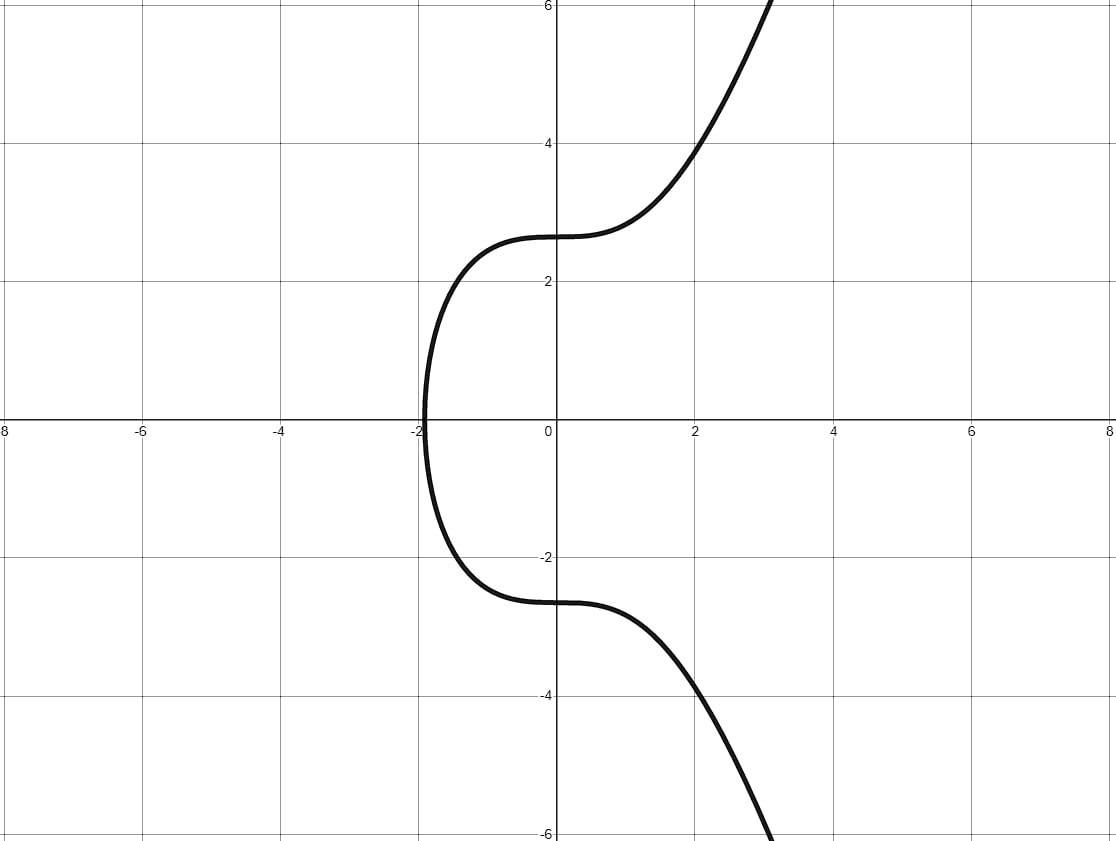
\includegraphics[scale=0.4]{img/secp256k1-curve.png}
  \caption{Représentation graphique de la courbe secp256k1 sur les nombres réels (source~: Loïc Morel, \emph{Bitcoin démocratisé}, 2022).}
  \label{fig:secp256k1}
\end{figure}

% Addition, multiplication par un scalaire, point de base
Une addition est définie sur cette courbe pour faire en sorte que la somme de deux points soit également un point de la courbe\sendnote{L'addition est définie par $P + Q = R$ où $x_R = \lambda_{P,Q}^2 - x_P - x_Q \pmod p$ et $y_R = \lambda_{P,Q}~( x_P - x_R ) - y_P \pmod p$ avec $\lambda_{P,Q} = \{ \frac{3 x_P^2}{2 y_P} \pmod p~\mathrm{si}~P = Q~;  \frac{y_Q - y_P}{x_Q - x_P} \pmod p~\mathrm{sinon} \}$.}. La multiplication par un scalaire est définie comme étant le fait d'additionner le même point à plusieurs reprises~: $m~P = P + \ldots + P~(m~\mathrm{fois})$. En fixant un point sur la courbe, appelé point de base et noté $G$\sendnote{Le point de base de secp256k1 est~: {\scriptsize \begin{align*} G = &~(~\mathtt{0x79be667ef9dcbbac55a06295ce870b07029bfcdb2dce28d959f2815b16f81798}, \\&~\mathtt{0x483ada7726a3c4655da4fbfc0e1108a8fd17b448a68554199c47d08ffb10d4b8}~)~. \end{align*}} Il a pour ordre le nombre premier {\scriptsize\[n = \mathtt{0xfffffffffffffffffffffffffffffffebaaedce6af48a03bbfd25e8cd0364141}~,\]} de sorte que $n~G = 0$.}, on peut définir une opération transformant un entier $d$ en un point de la courbe~: $Q = d~G$.

Ces opérations peuvent être représentées géométriquement sur la courbe. Par exemple, l'équivalent géométrique du doublement du point $G$ (addition avec lui-même) consiste à tracer la tangente du point, à considérer l'intersection de cette tangente avec la courbe et à en prendre l'opposé, comme représenté sur la figure~\ref{fig:secp256k1-multiplication}. Toutes ces opérations sont non réversibles.

\begin{figure}[h]
  \centering
  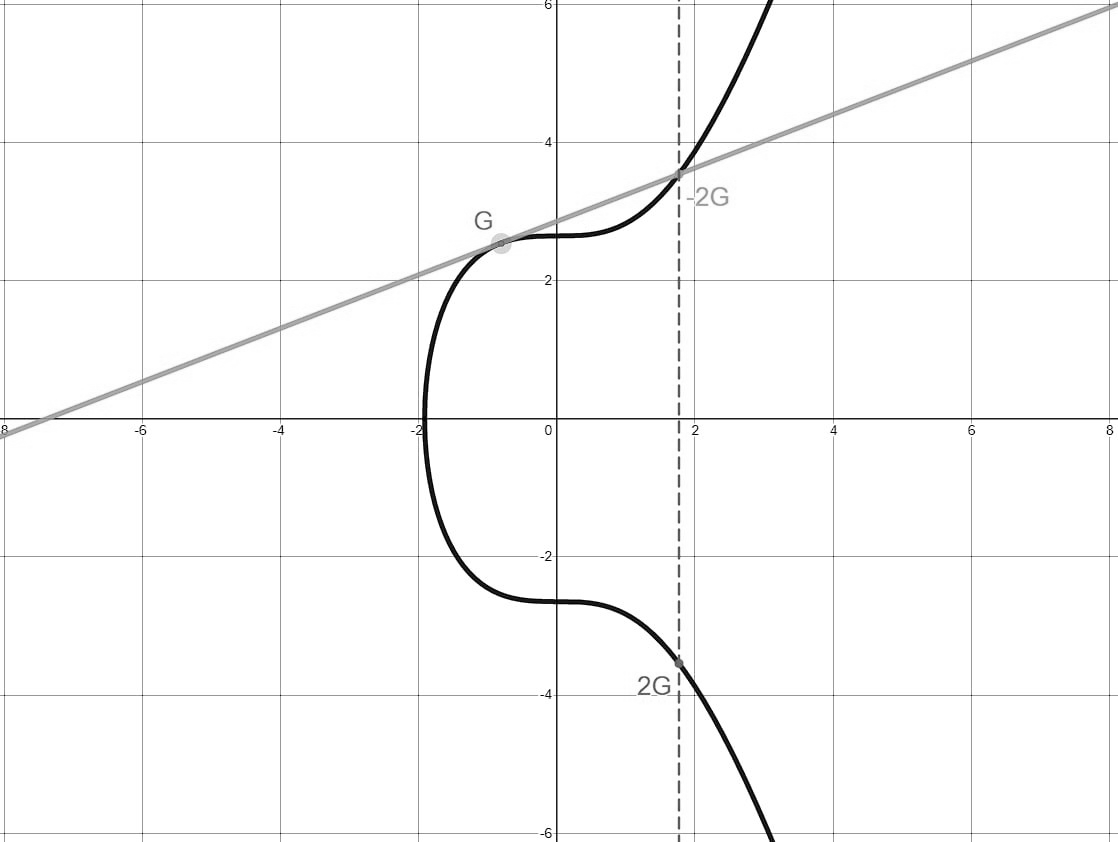
\includegraphics[scale=0.4]{img/secp256k1-multiplication.png}
  \caption{Représentation géométrique du doublement du point G sur secp256k1 (source~: Loïc Morel, \emph{Bitcoin démocratisé}, 2022).}
  \label{fig:secp256k1-multiplication}
\end{figure}

% Clé privée et clé publique.
En choisissant une clé privée $k$, on peut ainsi calculer la clé publique $K$ qui est $K = k~G$. Puisque la multiplication par un scalaire est non réversible, le passage de la clé privée à la clé publique constitue une fonction à sens unique. En d'autres termes, il est en pratique impossible de retrouver la clé publique à partir de la clé privée sans essayer chaque possibilité une à une.

% --- Clé privée ---

Regardons ce que cela donne en pratique. La clé privée est un nombre choisi aléatoirement. Elle doit être comprise entre $1$ et $n - 1$ où $n$ est l'ordre du point $G$ (qui approche $2^{256}$)~: 

{ \scriptsize
\[
n = \mathtt{0xfffffffffffffffffffffffffffffffebaaedce6af48a03bbfd25e8cd0364141}
\]
}

Par exemple, le nombre héxadécimal suivant est tout à fait valide pour servir de clé privée~:

{ \scriptsize
\[
k = \mathtt{0x999bb87eea489b2fc6219226e7b95d9083a3b627246ea852e85567ac4d72444f}
\]
}

% 6ef6b8ddb7d09b14a3f5239b1d76ed943bc697765ffd242baf08e532cdbe6197
% 5JfA14GGdTGCYWtfRmmv2dMNtwiHB2LHfzqcwMVi3BfzAx3GqhW
% KzwQjFQPytv5x6w2cLdF4BSweGVCPEt8b8HbcuTi8e75LRQfw94L

La clé publique est un point de la courbe défini par $K = k~G$. Si l'on calcule ce point à partir de la clé privée précédente, on obtient~:

{ \scriptsize
\begin{align*}
K = &~(~\mathtt{0xf6a6c7c39c88b767bfac4ac687c3ff32372e76c9fb633e2278e54472e300b3bd}, \\
    &~\mathtt{0x5822f24e0fdb4e568f97a7fff246c07ba486c1756f82971765cc9cf8e45ff5e6}~)
\end{align*}
}

% Représentation sérialisée
Dans Bitcoin, cette clé publique est représentée de manière sérialisée. Elle peut l'être sous forme non compressée, auquel cas elle est précédée par le préfixe \texttt{0x04}. Dans notre cas, son expression sérialisée est~:

\begin{Verbatim}[fontsize=\scriptsize]
04 f6a6c7c39c88b767bfac4ac687c3ff32372e76c9fb633e2278e54472e300b3bd
5822f24e0fdb4e568f97a7fff246c07ba486c1756f82971765cc9cf8e45ff5e6
\end{Verbatim}

% Représentation compressée
Il existe également une représentation compressée de la clé publique. Celle-ci est rendu possible par la symétrie de la courbe par rapport à l'axe des abscisses~: car en effet, le fait que le point $(x, y)$ appartienne à la courbe implique que le point $(x, - y)$ y soit aussi. Pour compresser l'information, il suffit ainsi de donner l'abcisse $x$ et un préfixe qui vaut \texttt{0x02} si $y$ est pair ou \texttt{0x03} si $y$ est impair\sendnote{Dans le corps fini $\mathbb{F}_p$, prendre l'opposé d'un élément non nul $y$ inverse sa polarité. En effet, si $y \in [\![ 1, p - 1 ]\!]$, alors $-y + p \in [\![ 1, p - 1 ]\!]$.}. On peut ensuite retrouver grâce à l'équation de la courbe. Dans notre cas, la clé publique compressée est~:

\begin{Verbatim}[fontsize=\scriptsize]
02 f6a6c7c39c88b767bfac4ac687c3ff32372e76c9fb633e2278e54472e300b3bd
\end{Verbatim}

Ce format permet de réduire la taille des transactions (et donc les frais)~: c'est pour cela qu'il est utilisé dans la plupart des portefeuilles récents, et qu'il est imposé dans le cas de SegWit. Le format non compressé tend ainsi à disparaître, même s'il reste toujours valide dans les transactions classiques.

Dans Bitcoin, la clé publique servait initialement à recevoir les fonds directement («~\eng{Pay to Public Key}~»), de sorte qu'on la confond encore aujourd'hui avec la notion d'adresse. Toutefois, c'est son empreinte obtenue par hachage («~\eng{Pay to Public Key Hash}~»), qui sert généralement d'adresse de réception, comme nous le décrirons plus bas.

% --- Signature ---

L'algorithme de signature ECDSA s'applique à un message $m$ qui est précédemment haché et produit une signature $(r, s)$. Il est ensuite possible de faire correspondre la signature avec la clé publique $K$ grâce à un algorithme de vérification qui ne nécessite pas de connaître la clé $k$\sendnote{L'algorithme de signature ECDSA est le suivant. En notant $H(m)$ l'empreinte cryptographique du message à signer, la signature est obtenue en appliquant les étapes suivantes~:

\begin{itemize}
  \item[$\bullet$] Choisir aléatoirement une clé éphémère $l$ inférieure à $n-1$~;
  \item[$\bullet$] Calculer les coordonnées $(i,j)$ du point $l~G$~;
  \item[$\bullet$] Calculer $r = i \mod n$~; si $r = 0$, choisir un autre $l$~;
  \item[$\bullet$] Calculer $s = l^{-1} ( H(m) + k r ) \mod n$~; si $s = 0$, choisir un autre $l$~;
  \item[$\bullet$] La signature est $( r, s )$.
\end{itemize}

L'algorithme de vérification est le suivant~:

\begin{itemize}
  \item[$\bullet$] Vérifier que $K \ne 0$ et que $K$ appartient à la courbe~;
  \item[$\bullet$] Vérifier que $n~K = 0$~;
  \item[$\bullet$] Vérifier que $1 \leq r \leq n - 1$ et $1 \leq s \leq n - 1$~;
  \item[$\bullet$] Calculer $(i, j) = ( H(m) s^{-1} \mod n )~G + ( r s^{-1} \mod n  )~K$~;
  \item[$\bullet$] Vérifier que $r = i \mod n$.
\end{itemize}}.

% Transaction et signature
Dans Bitcoin, le message est la transaction. L'agorithme de vérification montre ainsi que la personne qui a produit la signature connaît $k$ tel que $K = k~G$, c'est-à-dire qu'elle est propriétaire des bitcoins. C'est ce qui permet aux nœuds du réseau de s'assurer de la validité des signatures, et par conséquent de celle de la transaction. Un exemple de signature correspondant à notre clé publique et à une transaction réalisée sur le réseau principal est\sendnote{Il s'agit de la signature de la transaction d'identifiant \longstring{08e5ce0783ab6d5534e234136df02e0e240f76108eb6af04b8b624646b66f5eb}. Sous forme sérialisée (DER), cette signature est \longstring{3044022019b83a5e354ef62e98413e6ef3f37ad0c69f75cea7daa6a352cf66f4668a9a0b02204c13f9b6f2c8ea7af224b3f6a3d9cfdfe5085bbafa150fb1aa72a20ce7cac6b001}.}~:

{ \scriptsize
\begin{align*}
(r, s) = &~(~\mathtt{0x19b83a5e354ef62e98413e6ef3f37ad0c69f75cea7daa6a352cf66f4668a9a0b}, \\
    &~\mathtt{0x4c13f9b6f2c8ea7af224b3f6a3d9cfdfe5085bbafa150fb1aa72a20ce7cac6b0}~)
\end{align*}
}

% Autres algorithmes de signature
Notez que l'algorithme ECDSA présenté ici n'est pas le seul qui existe. En novembre 2021, BTC a intégré un autre algorithme, le schéma de signature numérique de Schnorr, qui est basé sur la même courbe elliptique mais qui apporte des bénéfices majeurs. Certaines autres variantes de Bitcoin comme Monero utilisent EdDSA, un algorithme de signature basée sur une courbe d'Edwards tordue.

\section*{Le hachage} % l'intégrité de l'information
\addcontentsline{toc}{section}{Le hachage}

Bitcoin fait également usage du hachage. Le hachage est un procédé cryptographique permettant de garantir l'intégrité d'une information numérique. Le nom de ce procédé est issu d'une analogie avec la cuisine, où des aliments peuvent être coupés en petits morceaux et regroupés dans un hachis. Il est mis en œuvre par une fonction de hachage qui transforme un \emph{message} de taille variable en une \emph{empreinte} de taille fixe. Cette empreinte est aussi appelé condensat ou \eng{hash}.

Les fonctions de hachage sont des fonctions déterministes, facilement exécutables, qui possèdent en théorie trois caractéristiques\sendnote{Il s'agit de suppositions et certaines fonctions satisfont ces caractéristiques plus que d'autres. Ainsi, des collisions ont été trouvées au sein des fonctions MD5 et SHA-1 alors qu'on les croyait sûres.}~:

\begin{itemize}
  \item[$\bullet$] Elles sont irréversibles~: ce sont des fonctions à sens unique construites de telle sorte qu'il est difficile de retrouver le message à partir d'une empreinte donnée (résistance à la préimage)~;
  \item[$\bullet$] Elles sont imprédictibles~: toute modification du message initial résulte en une empreinte profondément différente, si bien qu'il est difficile de trouver une empreinte similaire~;
  \item[$\bullet$] Elles sont résistantes aux collisions~: il est difficile de trouver deux messages dont l'empreinte résultante soit la même. 
\end{itemize}

L'une des fonctions les plus connues est SHA-256, dont le nom vient de l'abréviation de \eng{Secure Hash Algorithm} et de la taille des empreintes qu'elle produit (256 bits, soit 32 octets). Par exemple, si on considère le message «~Bitcoin~», le fait de l'orthographier en minuscules ou d'ajouter un point change complètement son empreinte, comme montré dans le tableau~\ref{table:sha256-hashes}. Cette particularité permet notamment de détecter si le message comporte une erreur.

\begin{table}[h]
  \begin{tabular}{| c | c |}
    \hline \footnotesize \textbf{Message} & \footnotesize \textbf{Empreinte (SHA-256)} \\
    \hline \footnotesize Bitcoin & \scriptsize \longstring{b4056df6691f8dc72e56302ddad345d65fead3ead9299609a826e2344eb63aa4} \\
    \hline \footnotesize bitcoin & \scriptsize \longstring{6b88c087247aa2f07ee1c5956b8e1a9f4c7f892a70e324f1bb3d161e05ca107b} \\
    \hline \footnotesize Bitcoin. & \scriptsize \longstring{a9adf3c04d168153b296083f05015f587d7df6e0b85305b6c7beb2a69e3f4e75} \\
    \hline
  \end{tabular}
  \caption{Empreintes par SHA-256 de messages légèrement différents.}
  \label{table:sha256-hashes}
\end{table}

Le hachage intervient à de multiples endroits dans Bitcoin~: dans l'algorithme de signature (hachage du message), dans le calcul des adresses, dans la dérivation des clés, pour le calcul des sommes de contrôle, pour le calcul des identifiants des transactions et des blocs, dans la construction des arbres de Merkle dans les blocs, et enfin au cœur du minage.

Trois fonctions de hachage sont utilisées~: SHA-256, qui produit des empreintes de 256 bits (32 octets)~; RIPEMD-160, dont le nom est le sigle de l'anglais \eng{RACE Integrity Primitives Evaluation Message Digest}) et qui résulte en des condensats de 160 bits~; et SHA-512, qui hache les données en des empreintes de 512 bits.

La fonction la plus présente est le double SHA-256 (noté SHA-256d ou HASH-256), qui intervient presque partout. Il est supposé que ce doublement mis en place par Satoshi avait pour rôle la protection contre les attaques par extension de longueur\pagenote{«~Il est supposé que ce doublement mis en place par Satoshi avait pour rôle la protection contre les attaques par extension de longueur~»~: \url{https://bitcoin.stackexchange.com/questions/6037/why-are-hashes-in-the-bitcoin-protocol-typically-computed-twice-double-computed/6042\#6042}.}. La composée de SHA-256 par RIPEMD-160 est utilisée pour la calcul des adresses. C'est le seul endroit où RIPEMD-160 intervient de manière substantielle\sendnote{«~Les adresses Bitcoin sont le seul endroit où le hachage de 160 bits est utilisé.~» -- Satoshi Nakamoto, \eng{Re: Stealing Coins}, \wtime{25/07/2010 20:48:01 UTC}~: \url{https://bitcointalk.org/index.php?topic=571.msg5754\#msg5754}.}. Enfin, SHA-512 intervient dans l'algorithme de dérivation des clés mis en place dans les portefeuilles.

\section*{Les clés privées}
\addcontentsline{toc}{section}{Les clés privées}

Par essence, la clé privée est une information numérique, c'est-à-dire un nombre. Plus précisément, il s'agit d'un très grand nombre compris entre $1$ et $n-1$, où $n$ est l'ordre du point $G$ et approche $2^{256}$ soit $1,1579 \times 10^{77}$. L'intervalle est considérablement grand, si bien qu'il est statistiquement impossible de tomber sur une même clé privée en la choisissant au hasard. À titre de comparaison, le nombre d'atomes dans l'univers observable est proche de $10^{80}$.

% --- Importance de l'entropie ---

La clé privée est créée au hasard, la plupart du temps grâce à des algorithmes générateurs de nombres pseudo-aléatoires permettant de reproduire le hasard de la manière la plus fidèle possible en informatique. Cette génération repose sur l'entropie informatique issue de l'appareil, c'est-à-dire la quantité d'aléatoire qu'il collecte par le biais de sources matérielles (variance du bruit du ventilateur ou du disque dur) ou de sources extérieures (mouvement de la souris, signaux du clavier, etc.) Les outils utilisés pour générer des clés privées sont le plus souvent considérés comme cryptographiquement fiables (CSPRNG). % Entropie de Shannon (théorie de l'information) = mesure de l'incertitude

% Importance du hasard
La caractère aléatoire du procédé est fondamental, constituant la base de la sécurité du modèle. Par exemple, une personne qui choisirait le nombre 1 comme clé privée ne pourrait jamais utiliser l'adresse correspondante, car la sécurité liée à cette clé est nulle. Tous les bitcoins qui seraient déposés sur cette adresse seraient instantanément débités par un programme spécialisé\sendnote{On peut observer l'adresse \longstring{1EHNa6Q4Jz2uvNExL497mE43ikXhwF6kZm} (correspondant à la clé 1) pour se convaincre qu'il ne s'agit pas d'un bon choix.}.

% Brain wallets
Il est en de même des \eng{brain wallets}, portefeuilles «~cérébraux~» reposant sur la mémorisation d'une information, qui sont souvent créés de manière non sécurisée. Les gens partent le plus souvent d'une phrase cohérente (comme une citation tirée d'un livre ou d'une chanson) de sorte à pourvoir la retenir facilement, puis la hachent et utilisent l'empreinte résultante en tant que clé privée. Cette manière de faire est hautement risquée en raison de la forte prévisibilité du langage humain et les adresses créées comme cela ont de bonnes chances d'être vidées, comme l'a montré une enquête de BitMEX Research\sendnote{BitMEX Research, \eng{Call me Ishmael}, 13 octobre 2020~: \url{https://blog.bitmex.com/call-me-ishmael/}.}.

% Hasard dans l'algorithme de signature
Cette importance du hasard se retrouve également dans l'algorithme ECDSA qui repose sur la génération d'une clé éphémère pour produire la signature. Dans le cas où cette valeur ne serait pas correctement générée, un attaquant pourrait déduire les clés privées à partir des signatures. C'est notamment ce qui s'est passé en août 2013, lorsqu'une vulnérabilité (CVE-2013-7372) a été découverte au sein la fonction SecureRandom de Java et a affecté la sécurité de plusieurs portefeuilles logiciels sur Android\sendnote{Bitcoin.org, \eng{Android Security Vulnerability}, 11 août 2013~:\url{https://bitcoin.org/en/alert/2013-08-11-android}.}. L'exploitation de cette faille a mené à la perte d'au moins 55,82 bitcoins, soit 5~200~\$ à l'époque\pagenote{«~la perte d'au moins 55,82 bitcoins~»~: Burt Wagner, \eng{Bad signatures leading to 55.82152538 BTC theft (so far)}, \wtime{10/08/2013, 22:53:13 UTC}~:\url{https://bitcointalk.org/index.php?topic=271486.msg2907468\#msg2907468}.}. % La même clé éphémère a été réutilisée dans plusieurs signatures (même r).

% --- Encodage des clés privées ---

Après avoir été générées, les clés privées doivent ensuite être encodées dans le but de faciliter leur transmission, pour l'import dans un portefeuille ou pour l'export. Dans Bitcoin, elles sont ainsi représentées grâce à l'encodage Base58Check. C'est pourquoi on parle parfois de \eng{Wallet Import Format} (WIF).

L'encodage d'une clé suit une série d'étapes simples. Tout d'abord, la clé est préfixée par l'octet de version \texttt{0x80} qui indique qu'il s'agit d'une clé privée. Puis, un suffixe \texttt{0x01} est ajouté (ou non) pour indiquer si l'on souhaite en dériver une clé publique compressée (ou non compressée). Dans le cas de notre clé-exemple, on obtient les octets suivants~:

\begin{Verbatim}[fontsize=\scriptsize]
80 999bb87eea489b2fc6219226e7b95d9083a3b627246ea852e85567ac4d72444f 01
\end{Verbatim}

Ensuite, la somme de contrôle est calculée en prenant les 4 premiers octets de l'empreinte par le double SHA-256 et ajoutée après l'ensemble~:

% 80 999bb87eea489b2fc6219226e7b95d9083a3b627246ea852e85567ac4d72444f 416ec36d

\begin{Verbatim}[fontsize=\scriptsize]
80 999bb87eea489b2fc6219226e7b95d9083a3b627246ea852e85567ac4d72444f 01
1dd28791
\end{Verbatim}

Enfin, le tout est encodé en base 58. Dans le cas «~compressé~», la clé commence toujours par un K ou un L. Ici, notre clé privée s'écrit~:

\begin{Verbatim}[fontsize=\small]
L2NJfKog9SEdoAkAkm8ZNYDcpWQop95orPepbhsTE2t5Bf1yFmYk
\end{Verbatim}

Dans le cas «~non compressé~» (de moins en moins utilisé), la clé commence toujours par un 5. Ici, notre clé privée devient~:

\begin{Verbatim}[fontsize=\small]
5JywJHwyuD4YSsErniGJkrDNi87kggSZNADCEkhRyRScqfMMTEt
\end{Verbatim}

\section*{Les adresses}
\addcontentsline{toc}{section}{Les adresses}

Dans Bitcoin, une adresse constitue en quelque sorte un numéro de compte servant à recevoir des fonds. Cette donnée est disponible publiquement sur la chaîne de bloc et n'importe qui peut en vérifier le solde. Néanmoins, un utilisateur peut générer autant d'adresses qu'il le désire afin de ne pas dévoiler l'entièreté de son activité.

De manière générale, une adresse est l'empreinte d'une clé publique (PKH), la clé publique elle-même (PK), ou bien l'empreinte d'un script (SH). Ici nous parlerons des adresses simples, dérivées de clés publique par hachage, qui sont les plus utilisées sur le réseau BTC.

Une adresse simple est obtenue par les hachages successifs de la clé publique sérialisée par les fonctions SHA-256 et RIPEMD-160. La composée de ces deux fonctions est communément appelée HASH-160. La fonction RIPEMD-160 a été choisie par Satoshi dans le but de diminuer la longueur des adresses, car elle produisait des empreintes de 20 octets au lieu des 64 octets d'une clé publique ou des 32 octets produits par SHA-256. En notant $A$ l'adresse, on a ainsi~:

{ \small
\[
A = \mathrm{HASH160}(~K~) = \mathrm{RIPEMD160}(~\mathrm{SHA256}( K )~)
\]
}

Puisque cette composée est elle-même une fonction de hachage, elle a pour particularité d'être de même une fonction à sens unique. Il est de ce fait virtuellement impossible de retrouver la clé publique à partir de l'adresse.

Le risque de collision est lui aussi statistiquement nul, même s'il y a moins d'adresses que de clés privées. La fonction de hachage RIPEMD-160 produit en effet des empreintes de 160 bits, et il existe par conséquent $2^{160}$ (environ $1,4615 \times 10^{48}$) adresses possibles, soit approximativement $8 \times 10^{28}$ fois moins d'adresses que de clés privées. Néanmoins ce nombre est suffisamment élevé pour que le risque de tomber par hasard sur la même adresse soit complètement négligeable\sendnote{Supposons qu'une population mondiale de 10~milliards d'êtres humains utilise Bitcoin activement de sorte que chaque individu génère 1~million d'adresses en moyenne. La probabilitié d'une collision serait alors de~:
\[
10^{16}~/~2^{160} \simeq 0.000000000000000000000000000000684~\%~.
\]
Même si un individu tentait de construire une machine spécialisée générant et vérifiant un trillion ($10^{18}$) d'adresses par seconde et fonctionnant en continu, la probabilité d'accéder à une adresse déjà utilisée serait toujours négligeable (de l'ordre de $10^{-21}$). Nos cerveaux ne sont pas faits pour nous représenter de tels nombres.}.

Comme une clé publique admet deux représentations sérialisées (compressée et non compressée), il est possible de calculer deux empreintes. Nous nous focalisons ici sur la représentation compressée. L'empreinte de notre clé publique compressée est~:

\begin{Verbatim}[fontsize=\footnotesize]
a18bd7f41b42c7cc6ebfa4de43e6b63248536ebc
\end{Verbatim}

On peut en dériver trois adresses de type différent~: une adresse traditionnelle, une adresse SegWit native et une adresse SegWit imbriquée. Dans les trois cas, le principe est le même, bien que l'usage spécifique de l'empreinte dans le protocole diffère.

L'adresse traditionnelle est obtenue grâce un encodage de l'empreinte en Base58Check avec l'octet de version \texttt{0x00}. À cause de cet octet de version, les adresses traditionnelles simples commencent toujours par un 1 (purement symbolique car il vaut 0 en base 58). Notre adresse est~:

\begin{Verbatim}[fontsize=\small]
1FjBKPQ7MTiPSDkJ2ZwPgAXUKQ8yoGbVJX
\end{Verbatim}

Ce type d'adresse est appelé P2PKH (\eng{Pay to Public Key Hash}) et a été le premier type d'adresse dans Bitcoin.

L'adresse SegWit native est encodée grâce au format Bech32. Celui-ci inclut un préfixe indiquant le réseau (\texttt{bc} pour BTC) et un séparateur (\texttt{1}). De manière similaire à l'encodage des adresses traditonnelles, il s'agit de prendre l'information brute (la «~charge utile~»), de la préfixer avec l'octet de version (\texttt{0x00} pour la première version de SegWit), de calculer une somme de contrôle et d'exprimer le tout dans la base appropriée, à savoir la base 32. Ce procédé fait que l'adresse résultante commencera toujours par \texttt{bc1q}. Dans le cas de notre empreinte de clé publique, on obtient~:

\begin{Verbatim}[fontsize=\small]
bc1q5x9a0aqmgtrucm4l5n0y8e4kxfy9xm4udhygr2
\end{Verbatim}

Ce type d'adresse est appelé P2WPKH (\eng{Pay to Witness Public Key Hash}).

Enfin, on peut également inclure cette donnée sous la forme d'un script dans une adresse P2SH, créant une adresse SegWit dite «~imbriquée~». Le script, composé de l'octet de version de SegWit (\texttt{0x00}) et de l'empreinte, est haché pour constituer la nouvelle adresse. Comme dans le cas de toutes les adresses P2SH, l'empreinte résultante est encodée en Base58Check avec l'octet de version \texttt{0x05}. Cet octet de version a pour conséquence de faire commencer l'adresse par un 3. Notre empreinte devient ici~:

\begin{Verbatim}[fontsize=\small]
3JqPHkGuvW7nsUJDgm5CPSNUb47WczCC5e
\end{Verbatim}

Ce type d'adresse est appelé P2SH-P2WPKH (\eng{P2SH-nested Pay to Witness Public Key Hash}). Nous aborderons plus en détail les différents schémas de script qui sous-tendent ces types d'adresse dans le chapitre~\ref{ch:rouages}.

Une fois qu'elles ont été encodées, les adresses peuvent être partagées facilement d'une personne à une autre. Grâce à la somme de contrôle, faire une faute de frappe ne crée théoriquement pas de risque, car le logiciel la détectera et refusera de procéder au paiement. Les adresses sont aussi souvent représentées par des codes QR (voir figure~\ref{fig:address-qr-codes}), plus adaptés pour l'interaction avec un téléphone multifonction.

\begin{figure}[h]
  \centering
  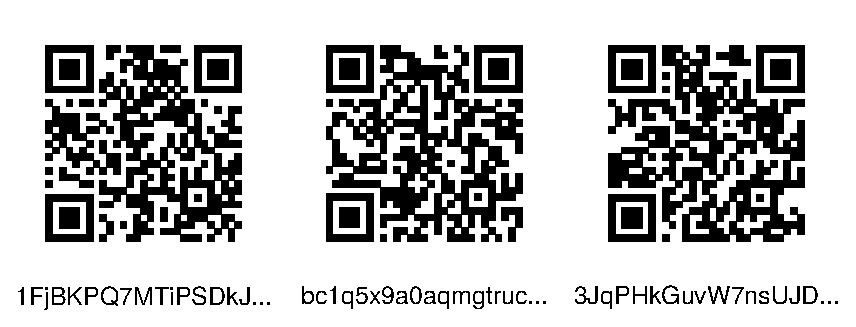
\includegraphics[scale=0.7]{img/address-qr-codes.eps}
  \caption{Codes QR des adresses.}
  \label{fig:address-qr-codes}
\end{figure}

En résumé~: lorsqu'un utilisateur veut recevoir un paiement, il génère une clé privée, en dérive une clé publique et crée à partir de celle-ci une adresse~; il communique son adresse à un autre utilisateur qui lui envoie des fonds~; il peut ensuite dépenser les fonds reçus en signant une transaction à l'aide de sa clé privée. Le réseau pair-à-pair de Bitcoin vérifie alors que la signature est conforme à la clé publique. 

La clé publique n'est révélée au réseau que lors de la transaction. Cela implique que les fonds sont protégés face à l'éventualité d'une mauvaise implémentation de l'algorithme de signature (comme dans le cas de l'exploitation de la faille au sein de SecureRandom en 2013) ou de la compromission généralisée d'ECDSA (par un ordinateur quantique par exemple). Il s'agit d'un bénéfice secondaire issu de l'utilisation de nouvelles adresses à chaque paiement.

Au-delà de BTC, les autres cryptomonnaies ont leur encodage propre pour les adresses, qui n'est souvent qu'une variante du standard modifiant la version ou le préfixe. Ainsi, dans Litecoin, les adresses traditionnelles commencent par un \texttt{L} (comme par exemple \longstring{LZx8abhwS7xSh2STChvgxBbEXcWG1AZ2iR}) et les adresses SegWit par un \texttt{ltc1q} (comme par exemple \longstring{ltc1q5x9a0aqmgtrucm4l5n0y8e4kxfy9xm4uft7vm6}).

Bitcoin Cash possède également son propre format d'adresse, appelée CashAddr, qui s'inspire fortement du format Bech32. Ce format a été introduit pour différencier les adresses BTC des adresses BCH. Une adresse BCH est simplement une représentation alternative du type P2PKH~: dans ce format, l'adresse \longstring{1FjBKPQ7MTiPSDkJ2ZwPgAXUKQ8yoGbVJX} devient \longstring{bitcoincash:qzsch4l5rdpv0nrwh7jduslxkceys5mwhs03g7e6dq}.

\section*{Les portefeuilles}
\addcontentsline{toc}{section}{Les portefeuilles}

% --- Portefeuille ---

Un portefeuille, de l'anglais \eng{wallet}, parfois aussi qualifié de portemonnaie, est un procédé de stockage des clés privées donnant accès aux pièces de cryptomonnaie de l'utilisateur. Ce procédé est souvent combiné avec la gestion de la cryptomonnaie~: sa réception avec la lecture de la chaîne de blocs et son envoi avec la production des signatures. Le moyen utilisé peut être une simple feuille de papier ou un fichier informatique, mais il s'agit généralement d'un logiciel sur mobile ou ordinateur, ou bien d'un appareil spécialisé.

Un portefeuille est donc par essence un \emph{porte-clés}. Son rôle principal est de conserver les clés privées dans le temps pour garantir la propriété des bitcoins. La plupart du temps, les clés sont générées par ces portefeuilles de manière déterministe à partir d'une phrase de récupération de 12 à 24 mots. L'utilisateur doit donc conserver précieusement cette phrase sur un autre support, dans l'éventualité de retrouver ses fonds si son appareil est perdu, cassé ou volé.

En revanche, un compte auprès d'un dépositaire comme une plateforme de change centralisée n'est pas un portefeuille à proprement parler, car ces services conservent les clés privées de leurs utilisateurs à des fins de sécurité et de facilité d'usage. Ainsi, des applications qui ressemblent à s'y méprendre à des portefeuilles, comme le \eng{Wallet of Satoshi} ou l'application Coinbase, n'en sont pas.

On peut classifier les portefeuilles existants en deux grandes catégories~: les portefeuilles «~à chaud~» (\eng{hot wallets}) qui sont connectés à Internet lors de leur utilisation, et les portefeuilles «~à froid~» (\eng{cold wallets}) qui ne le sont jamais de manière directe. De plus, on retrouve au sein de ces deux catégories différents types de portefeuilles, qui possèdent chacun leurs qualités et leurs défauts.

% --- Stockage à chaud ---

Le stockage à chaud des clés privées, qui utilise des appareils directement connectés à Internet, concerne notamment les portefeuilles logiciels (\eng{software wallet}) que l'on peut installer sur un mobile, une tablette ou un ordinateur généraliste. Ces logiciels mettent généralement leur code source à disposition du public pour des raisons évidentes de sécurité. Les clés sont conservées sur l'ordinateur et sont généralement chiffrées. Cette catégorie inclut les logiciels de nœud complet, les portefeuilles légers, les extensions de navigateur et les portefeuilles web.

L'implémentation de nœud complet (\eng{full node implementation}), aussi appelée client complet, est le premier type de portefeuille qui est apparu et le seul qui existait du temps de Satoshi. Comme son nom l'indique, un tel logiciel réalise toutes les opérations nécessaires au maintien d'un nœud sur le réseau pair-à-pair~: il télécharge l'intégralité de la chaîne de blocs et il vérifie et relaie les transactions non confirmées et les blocs. Bitcoin Core est le logiciel de nœud complet le plus connu. Cependant, en raison de la difficulté d'utilisation, ce type de portefeuille n'est généralement plus utilisé directement, les néophytes préférant utiliser des applications plus légères et les utilisateurs confirmés privilégiant des solutions plus sécurisées, qu'ils peuvent ensuite connecter à leur nœud personnel s'ils le souhaitent.

Le portefeuille léger (\eng{lightweight wallet}), aussi appelé portefeuille SPV, est un logiciel qui ne télécharge pas la chaîne de blocs mais qui procède à une vérification simplifiée des transactions à partir de la chaîne des entêtes qui ne nécessite que peu de ressources informatiques. Ce type de portefeuille est particulièrement adapté aux petits appareils comme les téléphones. Le logiciel peut interagir avec l'ensemble des nœuds complets du réseau pair-à-pair, comme le fait BRD (anciennement appelé \eng{breadwallet}), mais il passe de manière générale par l'intermédiaire d'une infrastructure de serveurs dédiés qui rendent l'utilisation plus agréable, comme c'est le cas d'Electrum ou de Samourai. Ce type de portefeuille garantit la sûreté des fonds, mais peut avoir un effet dommageable à d'autres niveaux, notamment en ce qui concerne la confidentialité. L'utilisateur peut également choisir de connecter son portefeuille à son propre nœud complet.

Un portefeuille peut aussi prendre la forme d'une extension de navigateur web, que ce soit sur Chrome, Firefox ou Brave. Contrairement aux clients légers, ces portefeuilles ne procèdent pas toujours à la vérification des transactions et font confiance au serveur auquel elles sont connectées.

Enfin, le dernier type de stockage à chaud est le portefeuille web. Ces derniers sont des interfaces en ligne permettant de gérer des fonds. Contrairement aux plateformes de change, l'utilisateur garde le contrôle de ses clés privées lorsqu'il passe par ce genre de service~: celles-ci sont gérées par le navigateur et ne sont jamais révélées à autrui. Le portefeuille de ce type le plus connu est celui de Blockchain.com.

% --- Stockage à froid ---

Mais ces solutions à chaud ne sont pas les seules, et il existe des méthodes de conservation à froid des clés privées, qui sont coupées de tout accès direct à Internet. Cette conservation a le mérite de réduire la surface d'attaque et donc le risque de vol par piratage informatique. Il s'agit de la solution recommandée pour mettre en sécurité des grosses sommes de cryptomonnaie.

Dans l'absolu, il faut disposer d'un appareil qui reste constamment hors-ligne pour générer les clés et les adresses. Cet appareil peut être un vieil ordinateur non connecté à Internet ou bien un appareil spécialisé. Les deux méthodes principales pour réaliser du stockage à froid sont le portefeuille papier et le portefeuille matériel.

Le portefeuille papier (\eng{paper wallet}) est le type de portefeuille le plus simple qu'on puisse imaginer~: les clés privées générées hors-ligne (et les adresses qui leur correspondent) sont écrites sur une feuille de papier. L'information écrite peut également être une phrase mnémotechnique. Le portefeuille papier présente néanmoins un inconvénient majeur~: l'impossibilité de signer des transactions sans l'importer dans une interface connectée à Internet. Cette méthode n'est pas du tout pratique, car l'utilisateur ne peut pas signer de transaction sans compromettre la sécurité de son portefeuille et doit se contenter de recevoir des paiements. Pour résoudre ce problème, il existe ce qu'on appelle les portefeuilles matériels.

Le portefeuille matériel (\eng{hardware wallet}) est un appareil dont la spécificité est de générer et de conserver les clés privées de manière isolée et de permettre de signer des transactions hors-ligne. Il s'agit aujourd'hui de la solution la plus sûre de détenir du bitcoin. Ces portefeuilles sont construits de telle manière que quelqu'un qui s'en emparerait ne pourrait pas dépenser les fonds sans le mot de passe de l'utilisateur.

Il existe une diversité de portefeuilles matériels. Les plus connus sont les portefeuilles de Satoshi Labs (le Trezor One et le Trezor model T) et ceux de Ledger (le Nano S et le Nano X), qui sont les modèles les plus anciens et les plus reconnus. Ceux-ci peuvent être connectés à l'ordinateur de manière sûre et les transactions sont toujours signées sur l'appareil. Certains autres perfectionnent la sécurité en étant physiquement isolés de tout ordinateur tiers (grâce à un air gap) comme la Cold Card Mk4. D'autres portefeuilles mettent l'accent sur la facilité d'utilisation comme les cartes Satochip qui se basent sur des smartcards.

Tous les portefeuilles impliquent une certaine confiance~: vous devez vous fier au logiciel que vous utilisez pour conserver vos bitcoins, au programme dont vous vous servez pour générer un portefeuille papier, au matériel spécialisé dans le stockage à froid. Bien entendu, les solutions ouvertes peuvent être considérées comme plus sûres dans le sens où d'autres personnes que les concepteurs ont pu vérifier le produit final~: c'est notamment le cas de nombreux portefeuilles logiciels et de l'infrastructure matérielle des portefeuilles Trezor\pagenote{«~l'infrastructure matérielle des portefeuilles Trezor~»~: \eng{Hardware design of Trezor}~:\url{https://github.com/trezor/trezor-hardware}.}. Dans tous les cas, une composante basée sur la réputation subsiste.

De manière générale, chaque type de portefeuille possède une utilité~: c'est donc à l'utilisateur de déterminer quel portefeuille conviendra mieux à ses besoins.

\section*{La dérivation des clés}
\addcontentsline{toc}{section}{La dérivation des clés}

% --- Phrase de récupération ---

Durant les débuts de Bitcoin, les clés privées étaient générées aléatoirement par le logiciel à chaque utilisation. Il s'ensuivait que les clés étaient conservées dans un fichier, appelé \texttt{wallet.dat}, stocké sur le disque dur de l'ordinateur. Cela rendait la perte des clés plus probable.

Néanmoins, les portefeuilles modernes ne fonctionnent plus comme cela. Les clés et les adresses sont dérivées de manière déterministe à partir d'une seule information générée aléatoirement, qui se présente sous la forme d'une phrase mnémotechnique allant de 12 à 24 mots. Ces mots peuvent être des mots en anglais, en français ou dans une autre langue.

% elder process crowd gentle proof taxi bean patient around warm source boil
% discuter ombrage cocasse exquis opale sodium asticot musicien amovible vaste rigide bancaire

\begin{quote}
elder process crowd gentle proof taxi bean patient around warm source boil
\end{quote}

De ce fait, c'est la conservation de cette phrase, appelée phrase de récupération, qui garantit la sécurité des bitcoins. Cette phrase vous permet de retrouver vos fonds si votre appareil est volé ou cassé. C'est pourquoi elle doit rester secrète. % aussi appelée «~graine~» (abus de langage)

Ce type de portefeuille est parfois appelé HD wallet pour \eng{Hierarchical Deterministic Wallet}~: portefeuille déterministe hiérarchique. Le concept a été développé pour Bitcoin à partir de 2011\pagenote{«~Le concept a été développé pour Bitcoin à partir de 2011~»~: Gregory Maxwell, \eng{Deterministic wallets}, \wtime{18/06/2011 21:27:29}~: \url{https://bitcointalk.org/index.php?topic=19137.msg239768\#msg239768}.}. Il a été standardisé en 2012 au sein du BIP-32 écrit par Pieter Wuille, et des propositions BIP-39 et BIP-44 écrites par Marek Palatinus et Pavol Rusnak. Il a été élargi aux autres cryptomonnaies en 2014\pagenote{«~Il a été élargi aux autres cryptomonnaies en 2014~»~: \eng{SLIP-0044 : Registered coin types for BIP-0044}~: \url{https://github.com/satoshilabs/slips/blob/master/slip-0044.md}.}.

% --- Génération de la phrase ---

En règle générale, la phrase secrète, ou phrase de récupération, est générée par l'appareil de l'utilisateur, qu'il s'agisse d'un téléphone mobile, d'un ordinateur ou d'un portefeuille matériel. Pour ce faire, une entropie est d'abord créée par l'appareil de manière pseudo-aléatoire. L'information, qui possède un nombre de bits précis, est ensuite enrichie d'une somme de contrôle de quelques bits, permettant de détecter les erreurs de saisie, et l'ensemble est divisé en segments de 11 bits. Enfin, chacun de ces segments est associé à un mot dans la liste standarde de 2048 mots, ce qui permet de former la phrase. Cette dérivation est représentée dans la figure~\ref{fig:from-entropy-to-mnemonic}.

Le nombre de mots de la phrase dépend de la taille de l'entropie désirée. Ainsi une entropie de 128 bits est dotée d'une somme de contrôle de 4 bits, ce qui donne une phrase de 12 mots de 11 bits. Pour 256 bits, on a une somme de contrôle de 8 bits et donc une phrase de 24 mots.

% entropy + checksum 010001110101010101110000110100010011000010011010110001011011110011000100111001010000100000001100001111101110011101000000000011001000
\begin{figure}[h]
  \centering
  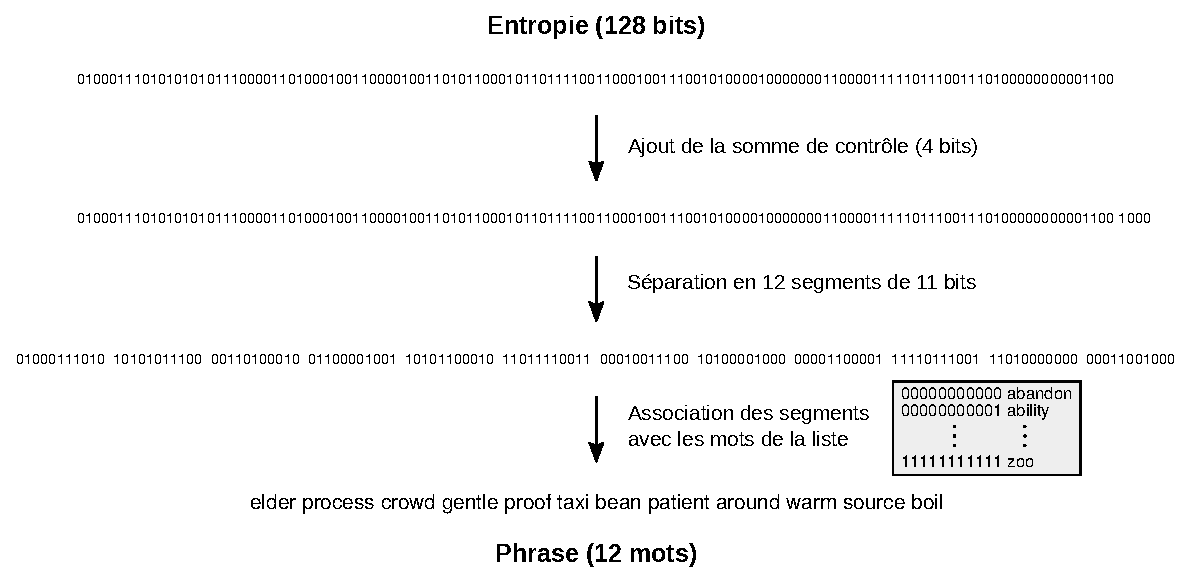
\includegraphics[scale=0.6]{img/from-entropy-to-mnemonic.eps}
  \caption{De l'entropie à la phrase secrète.}
  \label{fig:from-entropy-to-mnemonic}
\end{figure}

% --- Dérivation de la graine ---

Divers procédés cryptographiques sont utilisés pour dériver les clés et les adresses à partir de cette phrase. Ces procédés de dérivation ont sensiblement les mêmes propriétés que les fonctions de hachage en produisant des résultats irréversibles, imprédictibles et résistants aux collisions.

Le premier est le code d'authentification de message HMAC-SHA512 (HMAC pour \eng{Hash-Based Message Authentication Code}) qui calcule une empreinte en utilisant la fonction de hachage SHA-512 en combinaison avec une clé secrète. Le second est la fonction de dérivation de clé PBKDF2 (\eng{Password-Based Key Derivation Function 2}) qui applique de manière répétée une fonction choisie par l'utilisateur à un message de taille arbitraire avec un sel cryptographique.  L'intérêt est de nécessiter une quantité de calcul importante pour éviter un cassage par force brute de l'information supérieure.

Dans Bitcoin, PBKDF2 est utilisée pour dériver une graine à partir de la phrase mnénmotechnique, en appliquant la fonction HMAC-SHA512 à 2048 reprises. Le sel cryptographique est le terme \texttt{mnemonic} auquel on peut ajouter une phrase de passe (\eng{passphrase}) pour renforcer la sécurité du procédé. La graine résultante est une information de 512 bits (64 octets), à partir de laquelle la clé maîtresse et les clés suivantes sont dérivées.

% --- Dérivation des clés maîtresses ---

La dérivation des clés se fait grâce à la fonction HMAC-SHA512. Tout d'abord, on procède à une première dérivation à partir de la graîne. On applique le HMAC à la graine et au sel cryptographique \texttt{Bitcoin seed}, ce qui nous donne une clé maîtresse (premiers 256 bits du résultat) et un code de chaîne maître (derniers 256 bits du résultat). La passage de la phrase secrète à la clé maîtresse et au code de chaîne maître est résumé dans la figure~\ref{fig:from-mnemonic-to-root}.

% seed 219e07742e36087ff031070a3d843c9babb559bdbdbd55f6311ccec3c200ffce6e277eb858b656636b4e809c23f524fd4a21944d6841ee202caad8fda48508cb
% root (017c1714057a9821b167d1d0ffb549d02dc0fd0ca1bbce21990de09e07a4e9b2, 7e8edb2a43c93207d6a03fb9258af8052ce808971eb956ccccb14b2c5ddefa71)
\begin{figure}[h]
  \centering
  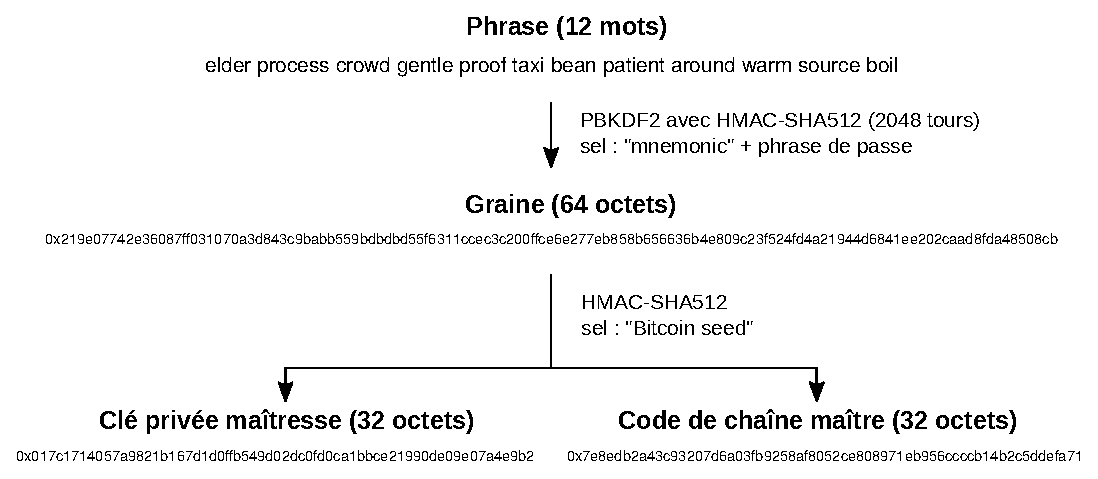
\includegraphics[scale=0.6]{img/from-mnemonic-to-root.eps}
  \caption{De la phrase secrète à la clé maîtresse.}
  \label{fig:from-mnemonic-to-root}
\end{figure}

% --- Clés étendues ---

Ces deux informations permettent de réaliser toutes les dérivations suivantes. Le code de chaîne intervient dans la chaîne de dérivation des clés, de sorte qu'il est impossible de procéder à la dérivation sans lui.

Plutôt que de gérer ces deux informations indépendemment, on préfère faire appel aux clés privées étendues (\eng{extended private keys}), qui incluent la clé privée et le code de chaîne, ainsi que d'autres informations comme la profondeur et l'indice de la clé enfant. La clé privée étendue est encodée en Base58Check avec un préfixe spécial qui dépend du type d'adresse dérivé, faisant que le résultat commence par \texttt{xprv} (adresses traditionnelles et clés Taproot), par \texttt{yprv} (adresses SegWit imbriquées) ou par \texttt{zprv} (adresses SegWit natives). Dans notre cas, la clé privée étendue issue de la clé privée maîtresse et du code de chaîne maître est~:

\begin{Verbatim}[fontsize=\footnotesize]
xprv9s21ZrQH143K3KSN1mSK8myNuDcXNvNoCDcU4KBxMTuj1Wo83zNn
jaj8dKFT81GttcgPftdB4XhAzzQLXJEGDtFp35yssYnxDV3yVDEqv1b
\end{Verbatim}

De même, la clé publique étendue (\eng{extended private key}) regroupe la clé publique et le code de chaîne correspondant à la clé privée dont elle dérive. En Base58Check, cette clé commence toujours par \texttt{xpub}, \texttt{ypub} ou \texttt{zpub}. La clé publique étendue correspondant à la clé privée maîtresse est~:

\begin{Verbatim}[fontsize=\footnotesize]
xpub661MyMwAqRbcFoWq7nyKVuv7TFT1nP6eZSY4rhbZuoShtK8GbXh3
HP3cUapsPsqEd52TRk1vhkgkhtAReezgSBi4ELh3YoxjmZgKBk7U98h
\end{Verbatim}

% --- Dérivation des clés ---

La dérivation des clés (\eng{child key derivation}) consiste à utiliser l'algorithme HMAC-SHA512 pour dériver des clés étendues «~enfant~» à partir d'une clé étendue «~parent~». Les codes de chaîne sont utilisés comme sel cryptographique. Deux types de dérivation existent~: la dérivation normale et la dérivation endurcie.

La dérivation normale fait intervenir la clé publique étendue dans le processus, ce qui rend possibles deux opérations~: l'obtention de la clé publique (étendue) enfant à partir de la clé publique (étendue) parent, et l'obtention de la clé privée (étendue) enfant à partir de la clé privée (étendue) parent. Le fonctionnement de ce type de dérivation est schématisé par la figure~\ref{fig:normal-child-key-derivation}.

\begin{figure}[h]
  \centering
  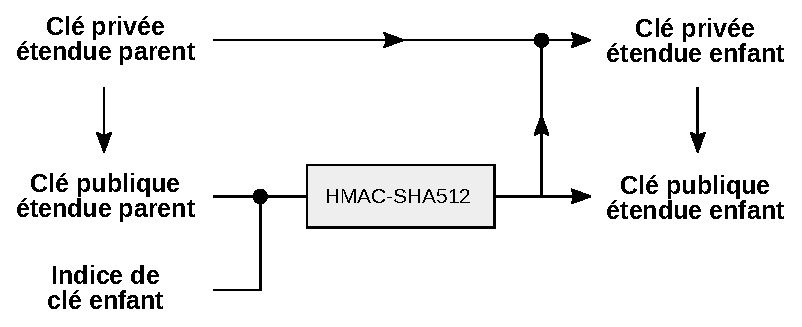
\includegraphics[scale=0.7]{img/normal-child-key-derivation.eps}
  \caption{Dérivation normale des clés par HMAC-SHA512.}
  \label{fig:normal-child-key-derivation}
\end{figure}

Cette particularité de la dérivation se révèle extrêmement utile pour générer de nouvelles adresses sans compromettre la clé privée racine. Un utilisateur peut ainsi importer la clé publique étendue dans un processeur de paiement afin de vérifier son solde et générer de nouvelles adresses sans avoir à fournir la clé privée. Cela permet aussi aux commerçants d'avoir des employés qui reçoivent des paiements à différentes adresses sans se soucier de la sécurité des fonds.

Cependant, cette particularité comporte un risque potentiel~: si une clé privée enfant est divulguée, alors la connaissance de la clé publique étendue parente (et donc du code de chaîne correspondant) permet d'obtenir toutes les clés privées enfant ainsi que la clé privée parent.

% Antonopoulos : "The ability to derive a branch of public keys from an xpub is very useful, but it comes with a potential risk. Access to an xpub does not give access to child private keys. However, because the xpub contains the chain code, if a child private key is known, or somehow leaked, it can be used with the chain code to derive all the other child private keys. A single leaked child private key, together with a parent chain code, reveals all the private keys of all the children. Worse, the child private key together with a parent chain code can be used to deduce the parent private key."

C'est pour cela qu'il existe un deuxième type de dérivation, la dérivation endurcie (\eng{hardened derivation}), qui, contrairement à la première, est restreinte au calcul de clés privées (étendues) enfant, ce qui assure une meilleure sécurité. Celle-ci est représentée dans la figure~\ref{fig:hardened-child-key-derivation}.

\begin{figure}[h]
  \centering
  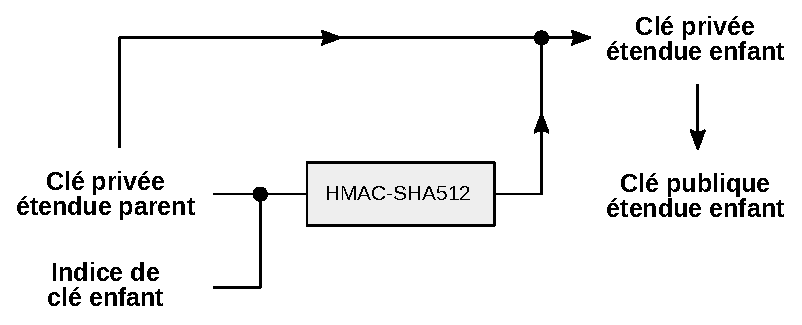
\includegraphics[scale=0.7]{img/hardened-child-key-derivation.eps}
  \caption{Dérivation endurcie des clés par HMAC-SHA512.}
  \label{fig:hardened-child-key-derivation}
\end{figure}

Chaque dérivation fait intervenir un indice, encodé sur 32 bits comme un entier signé, dont le bit de signe indique si elle doit être endurcie ou non et dont la valeur indique le numéro de la clé enfant. Ainsi, on peut produire 2~147~483~648 (de $0$ à $2^{31} - 1$) clés enfants normales et 2~147~483~648 clés enfants endurcies (de $-0$ à $- 2^{31} + 1$) à partir d'une même clé parent.

L'usage veut qu'on utilise une apostrophe pour désigner ce signe\sendnote{On utilise aussi parfois la lettre \texttt{h} (pour \eng{hardened}).}. L'indice \texttt{2} indique qu'il s'agit de la troisième clé enfant normale. L'indice \texttt{44'} indique qu'il s'agit de la 45\ieme{} clé enfant endurcie.

% --- Chemins de dérivation ---

Les dérivations successives permettent de créer des arbres de dérivation, dont la position de chaque clé peut être retrouvée grâce à un chemin, le chemin de dérivation. Ce dernier est composé des indices successifs des clés, qui sont séparés par des barres obliques (\texttt{/}). On le fait généralement commencer par la lettre \texttt{m} pour indiquer qu'on part de la clé privée maîtresse. Un exemple de chemin de dérivation est \longstring{m/84'/0'/0'/1/17}.

Chaque portefeuille peut utiliser son propre chemin de dérivation. Néanmoins, un standard a émergé, le BIP-44. Celui-ci simplifie la construction de portefeuilles à usages multiples, supportant plusieurs cryptomonnaies et donnant la possibilité de créer plusieurs comptes pour chacune d'entre elles\sendnote{Tous les portefeuilles ne respectent néanmoins pas ce standard. Le BRD wallet (ex Bread Wallet) utilise ainsi le chemin \texttt{m/0'} pour dériver le compte principal, conformément aux recommandations initiales du BIP-32.}.

Dans ce standard, on procède à trois dérivations endurcies puis à deux dérivations normales pour arriver à une clé privée et à l'adresse correspondante. Chaque dérivation apporte une information~:

\begin{itemize}
  \item[$\bullet$] La première dérivation (endurcie) sert à définir le but du portefeuille~: le 44 (qui fait référence au BIP-44) permet de dériver un compte utilisant des adresses traditionnelles, le 49 (BIP-49) pour les adresses SegWit imbriquées, le 84 (BIP-84) pour les adresses SegWit natives, le 48 ou le 45 (BIP-45) pour les adresses multisignatures, le 86 (BIP-86) pour dériver les clés publiques liées à Taproot,~etc.
  \item[$\bullet$] La deuxième dérivation (endurcie) indique le protocole cryptoéconomique et a fortiori les jetons liés~: le chiffre 0 est utilisé pour BTC, le 1 pour le testnet, le 2 pour LTC, le 60 pour ETH, le 128 pour XMR, le 145 pour BCH,~etc.
  \item[$\bullet$] La troisième dérivation (endurcie) donne l'indice du compte~: 0, 1, 2,~etc.
  \item[$\bullet$] La quatrième dérivation (normale) indique le rôle des adresses~: le 0 signale qu'il s'agit d'une adresse externe, dont le rôle est de réceptionner des bitcoins, le 1 d'une adresse interne, utilisée pour accueillir la sortie complémentaire lors d'un envoi de bitcoins (phénomène que nous décrirons dans le chapitre~\ref{ch:rouages})~;
  \item[$\bullet$] La cinquième dérivation (normale) donne de l'indice de la clé et de l'adresse considérée~: 0, 1, 2,~etc.
\end{itemize}

De ce fait, le chemin de dérivation ressemble à ceci~:

\begin{Verbatim}[fontsize=\footnotesize]
m / but' / protocole' / compte' / rôle_adresse / indice_adresse
\end{Verbatim}

Par exemple, la clé \longstring{m/44'/0'/0'/0/0} correspond à la première adresse de réception d'un compte Bitcoin utilisant les adresses traditionnelles. De même, la clé \longstring{m/84'/0'/0'/1/17} correspond à la 18\ieme{} adresse de reste du premier compte Bitcoin utilisant les adresses SegWit natives.

Toutes les adresses d'un portefeuille restent valides même si elles ont été utilisées. Même si l'on peut générer des adresses à l'infini, le portefeuille balaie usuellement 20 adresses à partir de la dernière adresse active.

\section*{La propriété dans Bitcoin}
\addcontentsline{toc}{section}{La propriété dans Bitcoin}

La propriété est le contrôle absolu exercé sur un bien par une personne à l'exclusion de toutes les autres. Bien souvent, la propriété s'exerce par l'intermédiaire d'un droit de propriété qui établit \eng{de jure} le rapport de force. Le bien possédé peut être un livre, une voiture ou un terrain. % usus, fructus, abusus

La propriété est à la base de la monnaie~: sans maîtrise réelle sur les unités monétaires, l'échange est impossible. En effet, la cession de pièces de métal précieux ou de billets fiduciaires requiert que le porteur les contrôle entièrement et puisse les abandonner au moment de la transaction. C'est pourquoi on parle aussi d'argent \emph{liquide}.

Sans cette propriété, les caractéristiques de la monnaie s'effritent. Aujourd'hui, l'essentiel des transactions a lieu par l'échange du crédit bancaire, que ce soit par le biais d'un paiement par carte bancaire, d'un virement ou d'un autre moyen numérique. Cette situation fait que les gens s'exposent de plus en plus aux formes de censure issues des contraintes réglementaires et de l'arbitraire bancaire, comme l'interdiction d'envoyer un virement ou le gel de compte sans préavis, outre le risque de solvabilité de la banque.

Bitcoin permet de redevenir pleinement propriétaire de son argent tout en conservant le côté numérique et immatériel de son usage. Cette propriété est de nature différente de celle exercée sur les objets~: elle est en effet indissociable de la connaissance exclusive d'une information (les clés privées) et de la protection de cette information.

Ainsi, l'information possède, plus que jamais, de la valeur. On a toujours associé une valeur au savoir en raison du pouvoir que ce dernier apporte (\eng{scientia potentia est}), mais cette valeur était indirecte. Aujourd'hui, une information peut procurer un accès direct à un certain montant de cryptomonnaie~: si quelqu'un connaît la clé privée qui correspond à une adresse contenant des bitcoins, il possède \emph{de facto} ces bitcoins.

Un utilisateur peut conserver du bitcoin extrêmement facilement en gardant en mémoire la clé privée ou la phrase de récupération. Il peut par exemple franchir une frontière étatique en ayant en sa possession un papier sur lequel se trouve l'information en question, ou bien tout simplement en la gardant en tête. C'est par exemple le cas d'un criminel allemand qui, après avoir miné frauduleusement 1~700 bitcoins en installant un logiciel sur des ordinateurs à l'insu de leurs propriétaires, a pu conserver sa fortune malgré son emprisonnement de deux ans\sendnote{Clément Wardzala, «~\emph{Bitcoin~: la police allemande à la recherche d'un mot de passe à 65 millions de dollars}~», \emph{Cryptoast}, 5 février 2021~: \url{https://cryptoast.fr/bitcoin-police-allemande-recherche-mot-de-passe-65m/}.}.

Un utilisateur peut recevoir des bitcoins en générant une nouvelle clé privée sur un appareil. Il ne nécessite aucune autorisation du réseau, même s'il doit bien entendu avoir accès à Internet pour vérifier les paiements entrants. En raison de la résistance du système à la censure, il peut faire ce qu'il veut de ses bitcoins~: financer des causes sensibles, acheter de la drogue sur le dark web, jouer au casino en ligne, envoyer des fonds à l'étranger,~etc. Il n'y a pas de limite de montant, ce qui confère à un individu fortuné un moyen d'avoir un impact autrement plus grand sur le monde.

\section*{Le risque de garde}
\addcontentsline{toc}{section}{Le risque de garde}

Même si Bitcoin permet l'échange libre au travers du cyberespace, il n'a pas fait disparaître les tiers de confiance pour autant. En effet, beaucoup de gens sont peu confiants dans leur capacité à conserver eux-mêmes leurs bitcoins, et préfèrent déléguer cette responsabilité à des services dépositaires, comme les services de garde spécialisés, les places de marché en ligne ou les applications de paiement. Il est aussi plus pratique de passer par une banque pour prêter son argent et le faire fructifier, ce qui profite aux plateformes de prêt en ligne.

% Pas vos clés, pas vos bitcoins
Bien que ce comportement se comprenne, il faut insister sur le fait que ceux qui épargnent des bitcoins par l'intermédiaire d'un dépositaire ne possèdent pas réellement ces bitcoins. La créance qu'ils possèdent sur le tiers de confiance n'est pas la propriété des bitcoins, puisque c'est le tiers en question qui les garde en son pouvoir. La loi étatique peut intervenir, mais cela n'empêche pas ce contrôle réel de s'exprimer dans une multitude de cas. C'est le sens de l'adage «~pas vos clés, pas vos bitcoins~» («~\eng{not your keys, not your coins}~»), popularisé par Andreas Antonopoulos\sendnote{Andreas Antonopoulos, \eng{Bitcoin Q\&A: How Do I Secure My Bitcoin?} (vidéo), 7 juillet 2017~: \url{https://www.youtube.com/watch?v=vt-zXEsJ61U}.}, qui rappelle que celui qui ne gère pas lui-même ses clés privées, ne possède pas réellement les bitcoins qu'il estime détenir. % En effet, si la délégation de la propriété donne certains avantages, elle a aussi ses inconvénients et fait courir des risques à ceux qui y ont recours. % Cela fait que de nombreuses personnes ne profitent pas des avantages de Bitcoin, qui est un «~argent liquide électronique~» dont le rôle est de permettre «~aux paiements en ligne d'être envoyés directement d'une partie à l'autre sans passer par une institution financière\sendnote{Satoshi Nakamoto, \eng{Bitcoin: A Peer-to-Peer Electronic Cash System}, 31 octobre 2008.}~».

Si la délégation de la propriété apporte certains avantages, elle a aussi ses inconvénients et fait courir des risques à ceux qui y ont recours. Tout d'abord, les dépositaires peuvent faire faillite dans le cas où leurs réserves deviennent trop basses pour les demandes de retrait. En cas de faillite, le client ne retrouve pas l'intégralité de ses fonds, à moins qu'une autre entité rachète les pertes de la plateforme.

Premièrement, cette faillite peut se matérialiser suite à une perte de fonds, comme ce qui est arrivé en juillet 2011 à la plateforme de change polonaise Bitomat qui avait perdu les clés privées liées à 17 000 BTC suite à un incident technique.

Deuxièmement, elle peut provenir d'un vol externe à la plateforme, issu par exemple d'un piratage, dont l'exemple le plus connu est le cas de la plateforme Mt. Gox qui a connu de multiples piratages entre 2011 et 2013 ayant mené à la volatilisation de 650~000 bitcoins, et qui a fait faillite en 2014\pagenote{«~la plateforme Mt. Gox qui a connu de multiples piratages entre 2011 et 2013 ayant mené à la volatilisation de 650~000 bitcoins, et qui a fait faillite en 2014~»~: Ludovic Lars, \emph{Mt. Gox et ses 842 109 bitcoins disparus, la lente descente aux enfers d'un géant du bitcoin}, 24 décembre 2020~:\url{https://journalducoin.com/analyses/mt-gox-lente-descente-enfers/}.}. La dette (en dollars) des créanciers de la plateforme devrait être remboursée en 2024, dix ans après les faits. % https://cryptoast.fr/mt-gox-dix-ans-apres-creanciers-enfin-rembourses/

Troisièmement, cette faillite peut résulter d'une escroquerie de sortie ou d'un vol interne, où le gestionnaire de la plateforme «~s'enfuit avec la caisse~». Ce type d'incident a été illustré en juillet 2011 par la fermeture du service MyBitcoin après le vol de 78~740 BTC par son fondateur anonyme Tom Williams. Un autre cas est celui de la plateforme canadienne QuadrigaCX, qui a fait faillite en 2019 suite à la mort de son fondateur et PDG, Gerald Cotten, qui s'avérait avoir dépensé les fonds pour financer son train de vie et son addiction à la spéculation. La faillite de la plateforme d'échange populaire FTX qui est survenue en novembre 2022 suite à l'utilisation frauduleuse des fonds de ses clients constitue un autre exemple explosif de ce type d'évènement.

Quatrièmement, même si aucune perte ou aucun vol de fonds ne survient, un fonctionnement par réserves fractionnaires du dépositaire peut le pousser à faire faillite à cause d'un resserrement du crédit. C'est notamment arrivé aux plateformes de prêt Celsius, Three Arrows Capital, Voyager Digital, BlockFi et Genesis Files en 2022--2023.

Ensuite, outre le risque de faillite, l'utilisation d'un dépositaire comporte le risque d'intervention étatique. La plateforme, pourvu qu'elle agisse sur le marché légal, se soumet aux diverses réglementations de LCB-FT et peut donc être amenée à geler un compte, voire à saisir les fonds qui s'y trouvent. C'est ce qu'a fait la place de marché Coinbase le 7 mars 2022 en bloquant 25~000 adresses dans le contexte des sanctions occidentales contre la Russie\sendnote{Paul Grewal, \eng{Using Crypto Tech to Promote Sanctions Compliance}, 7 mars 2022~: \url{https://blog.coinbase.com/using-crypto-tech-to-promote-sanctions-compliance-8a17b1dabd68}.}. La plateforme peut également être fermée par les pouvoirs publics, comme cela a été le cas de BTC-e en juillet 2017 qui a été saisie par le département de la Justice des États-Unis\sendnote{Department of Justice, \eng{Russian National And Bitcoin Exchange Charged In 21-Count Indictment For Operating Alleged International Money Laundering Scheme And Allegedly Laundering Funds From Hack Of Mt. Gox}, 26 juillet 2017~:\url{https://www.justice.gov/usao-ndca/pr/russian-national-and-bitcoin-exchange-charged-21-count-indictment-operating-alleged}.}.

Enfin, un autre inconvénient lié à l'utilisation d'un dépositaire est le cas des scissions, qui sont des duplications permanentes de la chaîne de blocs créant deux monnaies distinctes, et des \emph{airdrops} («~largages~»), qui sont des distributions gratuites de jetons à des fins publicitaires. Dans les deux cas, l'adresse de l'utilisateur est créditée d'un actif supplémentaire qui devient sa propriété. Cependant, si la personne passe par l'intermédiaire d'un dépositaire, ce dernier peut choisir de ne pas le lui céder, généralement d'une manière non frauduleuse, selon les critères déterminés par les conditions d'utilisation lors de l'inscription. En ce qui concerne les scissions, on peut citer l'exemple de la plateforme Bitstamp qui a refusé de céder les bitcoins SV de ses utilisateurs après la séparation entre BCH et BSV en novembre 2018 et qui continue de les conserver\sendnote{Patrick Thompson, «~\eng{Crypto exchanges delisting, denying access and stealing BSV}~», \emph{CoinGeek} 17 janvier 2020~: \url{https://coingeek.com/crypto-exchanges-delisting-denying-access-and-stealing-bsv/}.}. Pour les airdrops, on peut évoquer le cas de HEX, pyramide de Ponzi ouverte, dont la genèse en 2020 a été déterminée en partie par la possession de bitcoins~: chaque détenteur de bitcoin pouvait prétendre à un montant de jetons HEX proportionnel en publiant une signature numérique sur la chaîne d'Ethereum, mais il semble qu'aucune plateforme n'a pris le risque de tirer profit de ce largage.

La non-distribution des fruits des scissions et des \emph{airdrops} représente ainsi un manque à gagner, voire une perte sèche pour le client, surtout s'il s'agit d'une scission entre deux économies de taille équivalente. Toutefois, rien ne peut forcer en soi un dépositaire à proposer le retrait de ces gains, car la mise en œuvre technique a un coût non négligeable. Dans le cas contraire, les plateformes seraient contraintes de soutenir toutes les créations de ce type, y compris les plus fantaisistes, commes les scissions opportunistes de BTC qui ont eu lieu en 2017--2018 (Bitcoin Gold, Bitcoin Diamond, Bitcoin Private, etc.) % Ce refus peut s'apparenter à un vol si la plateforme bouge les pièces pour les revendre à son profit, mais tant qu'il n'y a aucun mouvement, on ne peut pas le déclarer.

D'une manière générale, le recours à un dépositaire comporte des inconvénients majeurs qui font qu'un utilisateur ne bénéficie pas de la résistance à la censure et de la résistance à l'inflation de Bitcoin. Conserver du bitcoin sur des plateformes réglementées permet à l'utilisateur de profiter vaguement de l'indulgence temporaire de l'État vis-à-vis des transferts et des plus-values réalisés. En outre, la généralisation de la garde de fonds présente un risque systémique comme nous le verrons. C'est pourquoi le recours aux dépositaires doit être considérée comme une exception, et non la règle, en ce qui concerne la conservation des bitcoins.

\section*{Propriété et responsabilité}
\addcontentsline{toc}{section}{Propriété et responsabilité}

Si Bitcoin permet à l'utilisateur de posséder son argent de manière souveraine, cette propriété s'accompagne d'une responsabilité. Cet utilisateur doit comprendre comment le système fonctionne, au moins de manière rudimentaire. Il doit choisir quels logiciels et quel matériel utiliser. Il doit manipuler les fonds, vérifier les adresses, rester vigilant à tout instant. Dans le cas d'une scission sans protection contre la rediffusion des transactions, il doit procéder lui-même à la séparation des pièces d'un côté et de l'autre. Il est seul face à l'incertitude, et surtout, face à lui-même. Cette responsabilité constitue le prix à payer pour la liberté monétaire.

Il est donc compréhensible que certaines personnes manquant de connaissances techniques, finissent par déléguer cette gestion, notamment dans le but de spéculer. Cependant, l'intérêt primordial de Bitcoin n'est pas de revenir à un système bancaire~: c'est de posséder pleinement ses fonds, sans que ceux-ci puissent être gelés par un tiers de confiance ou dilués par l'inflation monétaire. 

Puisque la sécurisation des bitcoins repose sur la connaissance d'une information, la conservation des bitcoins est inextricablement liée au dilemme qui existe entre la perte de données et la fuite de données. Pour conserver ses bitcoins, il faut à la fois garder l'accès à ses clés privées (éviter la perte de données) et en exclure les autres personnes (éviter la fuite de données), ce qui ne peut jamais être réalisé totalement.

Ce dilemme n'est résoluble que par un compromis entre la sécurité contre la perte et la sécurité contre le vol, qui est propre à chaque personne. Ainsi, quelqu'un peut simplement mémoriser sa phrase de 12 ou 24 mots pour conserver ses bitcoins, au risque de l'oublier et de les perdre définitivement. À l'inverse, une autre personne peut conserver des sauvegardes multiples à différents endroits au risque de voir un tiers d'accéder à l'une d'entre elles et de s'emparer de ses fonds.

D'un côté, nous avons le vol de bitcoins. Celui-ci peut se faire par un cambriolage~: une personne s'introduit chez autrui et s'empare du support physique sur lequel se trouve la sauvegarde ou le mot de passe. Mais il peut également être réalisé par intimidation~: les propriétaires sont attaqués physiquement pour être extorqués\pagenote{«~les propriétaires sont attaqués physiquement pour être extorqués~»~: Jameson Lopp maintient un registre (non exhaustif) des attaques physiques connues contre les propriétaires de bitcoins, où ceux-ci subissent des menaces de violences voire de torture afin de transférer des fonds~: \eng{Known Physical Bitcoin Attacks}, \url{https://github.com/jlopp/physical-bitcoin-attacks/blob/master/README.md}.}. La famille de Hal Finney a ainsi été ciblée par un maître-chanteur, qui lui a fait subir un swatting en réussissant à convaincre les unités spéciales de police d'intervenir en urgence au domicile familial\pagenote{«~La famille de Hal Finney a ainsi été ciblée par un maître-chanteur~»~: Robert McMillan, \eng{An Extortionist Has Been Making Life Hell for Bitcoin's Earliest Adopters}, 29 décembre 2014~: \url{https://www.wired.com/2014/12/finney-swat/}.}.

Il existe des bonnes pratiques pour ne pas s'exposer à ce type de vol. Tout d'abord, il est primordial de préserver sa confidentialité en évitant de déclarer qu'on possède des cryptomonnaies, combien on en possède, depuis combien de temps,~etc. Ce conseil s'applique également vis-à-vis des plateformes de change, qui connaissent l'identité de leurs clients et leurs adresses de retrait, et qui peuvent dévoiler ces informations suite à une requête étatique ou à une fuite.

Puis, l'utilisateur peut améliorer sa conservation. Il peut éviter de conserver ses sauvegardes dans les lieux les plus sensibles (comme son domicile). Il peut également répartir les fonds dans des portefeuilles gérés différemment afin d'atténuer l'impact d'un vol, bien que cela augmente également le risque de survenue de ce vol.

Il est ensuite possible de mettre en place un compte secondaire caché au sein d'un portefeuille matériel en exploitant l'utilisation de la phrase de passe. C'est une fonctionnalité que Ledger intègre dans ses produits\pagenote{«~C'est une fonctionnalité que Ledger intègre dans ses produits~»~: Ledger Documentation, \emph{Comment configurer une passphrase~?}~: \url{https://support.ledger.com/hc/fr-fr/articles/115005214529-Comment-configurer-une-passphrase-?}.}. Cette technique a le mérite de créer un «~déni plausible~» à présenter à l'assaillant qui menace ou qui torture le détenteur.

On peut enfin rendre la propriété des bitcoins collective, soit de manière explicite par la mise en place d'un compte multisignatures où chaque participant dipose de ses propres clés privées, soit de manière implicite par l'algorithme de partage de clés secrètes de Shamir (\eng{Shamir's Secret Sharing}). Cela permet d'impliquer d'autres personnes pour rendre l'extorsion plus difficile. 

De l'autre côté, nous avons la perte de bitcoins, qui représente le risque opposé de la conservation. La perte n'est pas en soi un problème pour le système. En effet, elle ne fait que renforcer le côté déflationniste du bitcoin~: comme le disait Satoshi Nakamoto, la perte ne fait qu'«~augmenter légèrement la valeur des pièces des autres~» et peut être considérée «~comme un don à tous\sendnote{Satoshi Nakamoto, \eng{Re: Dying bitcoins}, \wtime{21/06/2010, 17:48:26 UTC}~: \url{https://bitcointalk.org/index.php?topic=198.msg1647\#msg1647}.}~». Toutefois, il s'agit assurément d'un problème au niveau individuel, et la perte des clés a été pendant longtemps le principal risque pour l'utilisateur.

Certains des premiers mineurs ont ainsi perdu les bitcoins qu'ils avaient extrait. C'est le cas de James Howells, un ingénieur britannique qui a miné 8000 bitcoins pendant un peu plus de 2 mois en 2009 et qui a perdu la clé permettant d'y accéder\sendnote{James Howells a miné entre le 15 février (bloc $4334$) et le 24 avril 2009 (bloc $12~098$). Il a accumulé son revenu de minage à l'adresse \longstring{198aMn6ZYAczwrE5NvNTUMyJ5qkfy4g3Hi}. En date du 26 avril 2009, cette adresse contenait exactement 8000 bitcoins.}. Au cours de l'été 2013, il a en effet jeté son ordinateur contenant le fichier du portefeuille, en le déposant à la décharge publique près de chez lui. Il a réalisé son erreur quelques mois plus tard avec la hausse du cours et la médiatisation associée, mais il était trop tard. Son cas a été rendu public en novembre 2013 dans un article du \eng{Guardian}\sendnote{Alex Hern, «~\eng{Missing: hard drive containing Bitcoins worth £4m in Newport landfill site}~», \emph{The Guardian}, 27 novembre 2013~: \url{https://www.theguardian.com/technology/2013/nov/27/hard-drive-bitcoin-landfill-site}.}.

Un autre exemple (médiatisé en 2021\sendnote{Nathaniel Popper, «~\eng{Lost Passwords Lock Millionaires Out of Their Bitcoin Fortunes}~», \emph{The New York Times}, 12 janvier 2021~: \url{https://www.nytimes.com/2021/01/12/technology/bitcoin-passwords-wallets-fortunes.html}.}) est celui de Stefan Thomas, le programmeur allemand qui a été payé en bitcoins pour produire la première vidéo qualitative sur Bitcoin. Après avoir payé les frais pour cette vidéo, il a conservé le reste sur son portefeuille\sendnote{Les adresses de Stefan Thomas sont \longstring{1AYLzYN7SGu5FQLBTADBzqKm4b6Udt6Bw6} et \longstring{17eSZivDJpuJp9TxezTXVxkgLbsr3XZM1i}. En date du 8 juin 2011, leur solde combiné était de 7003,21 bitcoins.}. Il a procédé à une sauvegarde sur une clé USB chiffrée (IronKey) mais a fini par oublier son mot de passe de chiffrement.

% vivait en Suisse en 2011, est tombé sur Bitcoin en 2010 grâce à l'application StumbleUpon, a produit la vidéo "What is Bitcoin?" en mars 2011, focalisé sur les paiements

Les pertes sont donc courantes et il est nécessaire de se prémunir contre ce risque. L'adoption des portefeuilles déterministes hiérarchiques (\eng{HD wallets}), où les clés sont dérivées d'une seule phrase secrète, a grandement aidé à raffermir la sécurité contre la perte. Avant, on devait conserver un fichier contenant ses clés privées sur un appareil~; aujourd'hui la simple conservation de cette phrase suffit, ce qui facilite la copie sur un support physique.

La première mesure à mettre en place pour éviter la perte est la mise en place de sauvegardes multiples. L'utilisateur peut placer la phrase à différents endroits géographiques, si bien qu'il conserve la propriété de ses bitcoins en cas de sinistre de l'un de ces endroits (incendie, inondation, cyclone, etc.)  Il peut utiliser une feuille en papier simple ou cartonnée, ou bien il peut également faire le choix de graver ses mots sur une plaque d'acier forgée à cet effet\pagenote{«~graver ses mots sur une plaque d'acier forgée à cet effet~»~: Jameson Lopp, \eng{Metal Bitcoin Seed Storage Reviews}~: \url{https://jlopp.github.io/metal-bitcoin-storage-reviews/}.}.

L'utilisateur peut même, pour ses portefeuilles les moins fournis, conserver une sauvegarde numérique sur son ordinateur (si possible en la chiffrant) ou sur le \eng{cloud}, ce qui augmente sensiblement le risque de vol mais permet d'être sûr de pouvoir accéder aux bitcoins. Cet usage est généralement déconseillé, mais c'est à l'individu d'arbitrer la situation.

L'aspect programmable de Bitcoin peut également être mis à profit contre la perte. On peut ainsi mettre en place des systèmes de récupération de fonds, comme ce qui est fait par exemple dans le portefeuille Liana\sendnote{Jean-Luc (Bitcoin.fr), \eng{Sortie de la version 1.0 de Liana}, 12 mai 2023~: \url{https://bitcoin.fr/sortie-de-la-version-1-0-de-liana/}.}. Aucun standard de contrat de ce type ne s'est pour l'instant imposé, si bien que cette pratique reste déconseillée pour le novice. % Ludovic Lars, \eng{Wallet Recovery by a Third Party}, 25 août 2020~: \url{https://read.cash/@lugaxker/wallet-recovery-by-a-third-party-3693cfd9}.

Il peut être profitable pour l'utilisateur de tenir un ou plusieurs registres listant ses différents portefeuilles, même les plus anciens, afin de ne pas oublier où sont ses fonds. Cependant, encore une fois, il ne faut pas que ce registre soit trouvé, auquel cas les fonds pourraient être retrouvés plus facilement.

De même, on ne doit jamais supprimer la sauvegarde d'un portefeuille, même si ce dernier paraît vide. Celui-ci pourrait en effet contenir des cryptomonnaies issues de scissions ou pourrait recevoir des paiements à l'avenir (par exemple s'il inclut une adresse de donation publique). Il est en ce sens recommandé «~de le mettre de côté et de conserver l'ancienne copie au cas où\sendnote{Satoshi Nakamoto, \eng{Re: Version 0.3.13, please upgrade}, \wtime{03/10/2010 20:54:07 UTC}~: \url{https://bitcointalk.org/index.php?topic=1327.msg15136\#msg15136}.}~».

Enfin, l'utilisateur doit se souvenir qu'il va mourir. À moins qu'il ne veuille emporter ses possessions numériques dans sa tombe, il lui faut mettre en place un plan de succession pour ses bitcoins à destination de ses héritiers. Il existe de multiples manières de faire, mais le modèle le plus réputé est celui présenté par Pamela Morgan dans son \eng{Cryptoasset Inheritance Planning}\sendnote{Pamela Morgan, \eng{Cryptoasset Inheritance Planning}, Merkle Bloom LLC, 2018.}. Celui-ci consiste à écrire une lettre dans laquelle l'utilisateur inclut les coordonnées de gens de confiance à contacter pour aider ses héritiers (nos proches ne sont \emph{a priori} pas autant à l'aise que nous avec la manipulation de bitcoins) ainsi que l'inventaire de ses avoirs (dans le but de récupérer les sauvegardes et de restaurer les portefeuilles). La lettre est scellée et placée dans un lieu sûr, comme un coffre-fort personnel, un coffre en banque ou chez un notaire.

\section*{Bitcoin et l'information}
\addcontentsline{toc}{section}{Bitcoin et l'information}

Bitcoin permet donc pour la première fois dans l'histoire d'être propriétaire d'un bien numérique rival. Cette propriété s'exerce par la connaissance exclusive d'informations, les clé privées, qui sont générées et gérées par des outils appelés les portefeuilles. Grâce au procédé de signature numérique, ce sont en effet ces clés privées qui permettent de signer les transactions dépensant les bitcoins.

Couplée à la résistance à la censure, cette assurance de la propriété permet de réaliser des transactions librement sur Internet, sans craindre le gel de compte. Mais elle s'accompagne également d'une responsabilité qui impose à l'utilisateur de prendre un certain de nombres de mesures pour ne pas voir ses fonds disparaître.

Ainsi, le système de signatures numériques «~fournit un contrôle fort de la propriété~». Cependant, il «~reste incomplet sans moyen d'empêcher la double dépense\sendnote{Satoshi Nakamoto, \eng{Bitcoin: A Peer-to-Peer Electronic Cash System}, 31 octobre 2008.}~». C'est la résolution de ce problème qui constitue l'objet du prochain chapitre.
% Copyright (c) 2023 Ludovic Lars
% This work is licensed under the CC BY-NC-SA 4.0 International License

\chapter{Le consensus par le minage}
\label{ch:confirmation}

Bitcoin est un modèle décentralisé de monnaie numérique issu de l'informatique distribuée, une discipline développée au moment de l'émergence d'Internet. Il se fonde plus précisément sur un réseau pair-à-pair d'ordinateurs, dans lequel les participants possèdent tous les mêmes responsabilités. En tant que tel, il constitue un \emph{système d'argent liquide électronique pair-à-pair}.

Tout l'enjeu de Bitcoin est ainsi de se mettre d'accord sur le contenu d'un registre déterminant qui possède quoi, c'est-à-dire d'arriver à un consensus sur la propriété des unités. En particulier, l'établissement d'un tel accord permet de résoudre le problème de la double dépense, qui se pose dans le monde numérique en raison de la facilité de reproduction des données.

Le consensus -- accord unanime au sein d'un groupe de personnes -- n'est pas une chose facile à atteindre entre les êtres humains. La conciliation sociale peut fonctionner concernant des règles générales, mais n'est pas adaptée quant aux détails particuliers. C'est pourquoi les organisations humaines sont bien souvent obligées de s'en remettre à une autorité centrale chargée de prendre les décisions.

Bitcoin a précisément pour contrainte d'éviter le recours à un tiers de confiance. De ce fait, il repose sur un mécanisme de consensus distribué, que l'on appelle communément le minage, où la confirmation des transactions, c'est-à-dire leur inclusion dans le registre, est assurée par un procédé nommé la preuve de travail. Dans ce chapitre, nous détaillerons le fonctionnement de cet algorithme de consensus novateur.

% Le minage, en plus d'être la manière dont sont distribués les nouvelles unités (d'où son nom), est le moyen par lequel le réseau arrive à un consensus.

\section*{Le problème des généraux byzantins} % Le consensus distribué
\addcontentsline{toc}{section}{Le problème des généraux byzantins}

% --- Métaphore des généraux byzantins ---

L'enjeu du consensus est illustré par le problème des généraux byzantins, qui est un problème d'informatique distribuée formalisé en 1982 par Leslie Lamport, Robert Shostak et Marshall Pease\sendnote{Leslie Lamport, Robert Shostak, Marshall Pease, \eng{The Byzantine Generals Problem}, 1982~: \url{https://lamport.azurewebsites.net/pubs/byz.pdf}.}. Ce problème traite de la remise en cause de la fiabilité des transmissions et de l'intégrité des participants dans les systèmes distribués, et il s'applique dans les cas où les composants d'un système informatique ont besoin d'être en accord.

Le problème est énoncé sous la forme d'une métaphore faisant intervenir des généraux de l'armée de l'Empire byzantin, l'Empire romain d'Orient qui a subsisté jusqu'en 1453 suite à la chute de la partie occidentale en 476\sendnote{Selon Leslie Lamport, l'appellation byzantine a été choisie pour ne pas offenser le sentiment patriotique du lecteur (l'armée dans la métaphore comporte des traîtres), car cette appellation a été faite \emph{a posteriori} par les historiens et les Byzantins eux-mêmes se considéraient comme romains. -- Voir Leslie Lamport, \eng{My Writings}~: \url{http://lamport.azurewebsites.net/pubs/pubs.html\#byz}.}. Ces généraux assiègent une ville ennemie avec leurs troupes dans le but de l'attaquer. Ils ne peuvent communiquer qu'à l'aide de messages relayés oralement et ils doivent trouver un moyen d'établir un plan de bataille commun par ce moyen. Par exemple, les généraux peuvent chercher à coordonner une attaque à l'aube, et partagent leurs intentions entre eux en envoyant le message «~attaque~» par le biais d'un message pour confirmer l'assaut, et «~retraite~» pour l'annuler. % Le nom de cet empire fait référence à Byzance, le nom antique de sa capitale Constantinople (aujourd'hui Istanbul).

% La situation est la suivante. Des généraux de l'armée byzantine campent autour d'une cité ennemie avec leurs troupes et souhaitent l'attaquer. Ils ne peuvent communiquer qu'à l'aide de messagers oraux et doivent établir un plan de bataille commun. Pour prendre un exemple simple, les généraux peuvent chercher à coordonner une attaque à l'aube, et partagent leurs intentions entre eux en envoyant le message «~attaque~» pour confirmer l'assaut, et «~retraite~» pour l'annuler.

Cependant, un petit nombre de ces généraux s'avèrent être des traîtres au service de l'ennemi qui essaient de semer la confusion au sein de l'armée. Ces traîtres envoient ainsi des messages contradictoires à leurs interlocuteurs, pour faire en sorte que certains généraux loyaux attaquent, et que d'autres battent en retraite au moment de l'assaut, causant par là une défaite certaine, comme illustré sur la figure~\ref{fig:byzantine-generals-attack}.

\begin{figure}[h]
  \centering
  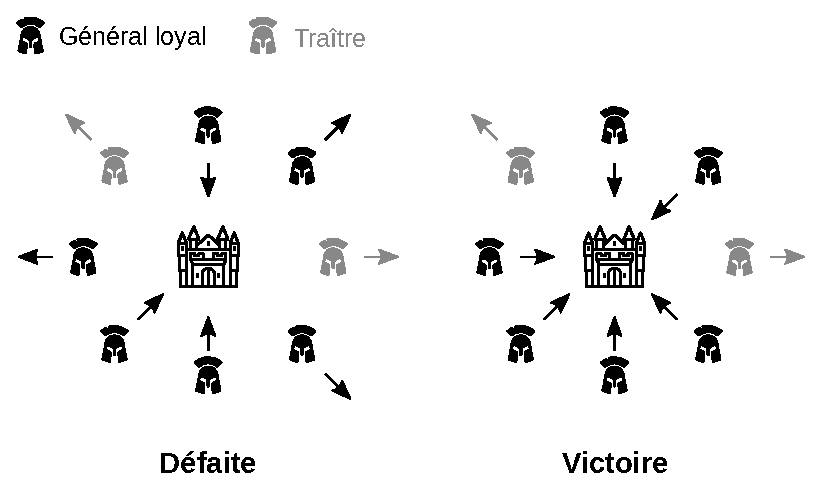
\includegraphics[scale=0.7]{img/byzantine-generals-attack.eps}
  \caption{Attaque des généraux byzantins contre la ville~: succès et échec.}
  \label{fig:byzantine-generals-attack}
\end{figure}

Le problème est de trouver une stratégie (c'est-à-dire un algorithme) permettant de s'assurer que tous les généraux loyaux se mettront d'accord sur le plan de bataille. Les traîtres battront alors en retraite, mais puisque leur nombre est supposément restreint, l'attaque sera quand même un succès.

La situation fait qu'il est difficile de parvenir à un consensus. On ne peut pas désigner un commandant auxquels les généraux subordonnés obéiront, car le commandant peut être lui-même un traître. Lamport, Shostak et Pease ont montré que le problème peut être résolu de manière absolue si (et seulement si) les généraux loyaux représentent strictement plus des deux tiers de l'ensemble des généraux\sendnote{Cette propriété est démontrée dans l'article original de Lamport et al. La condition plus précise est $n \ge 3 m + 1$ où $n$ est le nombre total de généraux et $m$ le nombre de traîtres.}~; autrement dit, qu'il ne peut pas y avoir plus d'un tiers de traîtres au sein de l'armée.

% Abstract: "Reliable computer systems must handle malfunctioningcomponents that give conflicting information to different parts of the system. This situation can be expressed abstractly in terms of a group of generals of the Byzantine army camped with their troops around an enemy city. Communicating only by messenger, the generals must agree upon a common battle plan. However, one or more of them may be traitors who will try to confuse the others. The problem is to find an algorithm to ensure that the loyal generals will reach agreement. It is shown that, using only oral messages, this problem is solvable if and only if more than two-thirds of the generals are loyal; so a single traitor can confound two loyal generals. With unforgeable written messages, the problem is solvable for any number of generals and possible traitors. Applications of the solutions to reliable computer systems are then discussed."

% --- Application de la métaphore aux systèmes distribués ---

La métaphore des généraux byzantins s'applique directement aux systèmes distribués, c'est-à-dire aux systèmes dont les composants sont séparés et doivent communiquer les uns avec les autres pour se synchroniser. Les généraux représentent les composants du système, les traîtres les composants défaillants, et les messages les données transmises entre les composants. Le but est d'obtenir un algorithme permettant de détecter les défaillances, appelées pannes byzantines, et de permettre aux autres composants de les écarter. La résilience obtenue est appelée la tolérance aux pannes byzantines~; le système est dit BFT, pour \eng{Byzantine Fault Tolerant}.

Le problème a été initialement décrit pour les systèmes informatiques reposant sur des composants présents à différents endroits et dans lesquels la bonne transmission des données est critique, comme les systèmes aéronautiques ou aérospatiaux\sendnote{L'infrastructure du Boeing 777 repose notamment sur le bus informatique ARINC 629 qui réplique en quadruple les messages envoyés afin de garantir un résultat avec une latence très faible. -- Elaine Ou, \eng{Byzantine Fault Tolerant Airplanes}, 12 février 2017~: \url{https://elaineou.com/2017/02/12/byzantine-fault-tolerant-airplanes/}.}. Mais il concerne aussi (ce qui nous intéresse ici) les systèmes pair-à-pair reposant sur un réseau horizontal de participants, et en particulier les systèmes cryptoéconomiques comme Bitcoin, dans lesquels les nœuds du réseau ont besoin de se mettre d'accord sur le contenu d'un registre. L'objectif est alors de trouver un algorithme permettant à tous les nœuds honnêtes de parvenir à un consensus en présence de nœuds traîtres (dits «~byzantins~»).

% replicated state machine
% réplication de machine à état (state machine replication) 

% --- Algorithmes de consensus classiques ---

Avant Bitcoin, le problème était résolu par des algorithmes dits «~classiques~» basés sur les idées de Lamport, Shostak et Pease. Le plus connu est probablement l'algorithme de consensus PBFT (pour \eng{Practical Byzantine Fault Tolerance}), mis au point par Miguel Castro et Barbara Liskov en 1999\pagenote{«~l'algorithme de consensus PBFT [...] mis au point par Miguel Castro et Barbara Liskov en 1999~»~: Miguel Castro, Barbara Liskov, \eng{Practical Byzantine Fault Tolerance}, février 1999.}, qui permettait à un nombre donné de participants de se mettre d'accord en gérant des milliers de requêtes par seconde avec une latence de moins d'une milliseconde.

Bien avant Bitcoin, Wei Dai et Nick Szabo envisageaient d'utiliser ce type d'algorithme pour leurs systèmes de monnaie électronique, b-money et bit gold. De même, de nombreux systèmes cryptoéconomiques en font encore aujourd'hui usage pour des raisons de performance, à l'instar d'Ethereum dont le consensus est basé sur l'algorithme Casper FFG. % comme nous l'avons vu dans le chapitre~\ref{ch:cybermonnaie}

Cependant, ces algorithmes impliquent des contraintes fortes~: les nœuds doivent connaître l'ensemble des autres nœuds et ils doivent communiquer avec tous les autres. De ce fait, il faut sélectionner les nœuds ayant le droit de participer au consensus avant de lancer l'algorithme, ce qui se fait généralement par preuve d'autorité (\eng{proof of authority}), via une liste blanche de nœuds, ou par preuve d'enjeu (\eng{proof of stake}), via un montant de jetons possédés ou délégués. Cela implique une moins bonne robustesse du système, car les validateurs sont alors connus de tous et donc davantage exposés aux attaques.

% La communication entre les nœuds du réseau doit être quadratique (chaque nœud doit communiquer avec tous les autres), ce qui fait qu'il est difficile de dépasser les 10 000 nœuds.

% --- Algorithmes de consensus de Bitcoin ---

Bitcoin résout ce problème d'une manière différente, grâce à un nouveau type d'algorithme~: l'algorithme de consensus de Nakamoto par preuve de travail. Celui-ci est plus robuste dans le sens où les nœuds du réseau n'ont pas besoin de connaître l'ensemble des autres nœuds et où aucune identification n'est requise.

Puisque le rôle principal de Bitcoin est le transfert de valeur, l'objectif est de se mettre d'accord sur qui possède quoi, c'est-à-dire sur l'\emph{état} du système. La solution proposée par Satoshi Nakamoto consiste à employer un registre recensant l'intégralité des transactions réalisées depuis le lancement du système, «~la seule façon de confirmer l'absence d'une transaction [étant] d'être au courant de toutes les transactions\sendnote{Satoshi Nakamoto, \eng{Bitcoin: A Peer-to-Peer Electronic Cash System}, 31 octobre 2008.}~». Ce registre formant l'\emph{historique} du système est organisé comme une succession de blocs de transactions, de sorte qu'il est communément appelé la \emph{chaîne de blocs}. Les nœuds du réseau entretiennent chacun une copie complète de la chaîne dont ils se transmettent des éléments sur demande.

Les nouveaux blocs sont ajoutés à la chaîne de manière régulière grâce à la production d'une preuve de travail. Les acteurs réalisant cette opération sont appelés des mineurs. Les nœuds du réseau arrivent à un consensus en considérant que la chaîne la plus longue est la chaîne correcte. Ainsi, comme l'a écrit Satoshi Nakamoto~:

\begin{quote}
«~La chaîne de preuves de travail est une solution au problème des généraux byzantins.\sendnote{Satoshi Nakamoto, \eng{Re: Bitcoin P2P e-cash paper}, \wtime{13/11/2008, 22:56:55 UTC}~: \url{https://www.metzdowd.com/pipermail/cryptography/2008-November/014849.html}.}~»
\end{quote}

La spécificité novatrice de cet algorithme est qu'il résout le problème de manière probabiliste plutôt que de manière absolue\sendnote{Plus précisément, il s'agit de sacrifier un peu de la propriété de sécurité au sens de Lamport pour améliorer la tolérance aux pannes byzantines.}. Par conséquent, les transactions incluses dans le registre ne sont jamais strictement finales, mais sont (probabilistiquement parlant) considérées comme telles au bout d'un temps. Ce fonctionnement permet de n'avoir besoin que de 51~\% de validateurs honnêtes, au lieu des 67~\% requis par les algorithmes classiques.

% Il s'agit d'un système de comptabilité à triple entrée\sendnote{Ian Grigg, \eng{Triple Entry Accounting}, 25 décembre 2015~: \url{https://iang.org/papers/triple_entry.html}~; Ian Grigg, \eng{Is BitCoin a triple entry system?} 13 juin 2011~: \url{http://financialcryptography.com/mt/archives/001325.html}.}, où le mécanisme de consensus joue le rôle de la tierce partie chargée d'assurer les transactions réalisées entre deux utilisateurs.

% La solution est moins efficace mais plus robuste. 

\section*{La preuve de travail}
\addcontentsline{toc}{section}{La preuve de travail}

% --- Description et historique du procédé ---

La preuve de travail, de l'anglais \eng{proof of work}, est un procédé permettant à un appareil informatique de démontrer de manière objective et quantifiable qu'il a dépensé de l'énergie. Ce moyen est utilisé pour sélectionner les ordinateurs dans le cadre de l'accès à un service ou à un privilège.

La preuve de travail est un mécanisme de résistance aux attaques Sybil, qui rend difficile la multiplication des identités à l'excès par un acteur qui chercherait à prendre le contrôle du réseau. Une attaque Sybil\pagenote{«~attaque Sybil~»~: Voir John R. Douceur, «~\eng{The Sybil Attack}~», in \eng{Peer-to-Peer Systems}, 2002, pp. 251--260. La pratique a été décrite en 1993 par le cypherpunk L. Detweiler sous le nom de \eng{pseudospoofing}~: \url{https://cypherpunks.venona.com/date/1993/10/msg00760.html}.} est une attaque intervenant au sein d'un réseau ouvert basé sur un système de réputation qui consiste à dupliquer les profils à moindre coût pour en altérer le fonctionnement. C'est par exemple un problème particulièrement présent sur les médias sociaux, où les comptes de robots sont utilisés en masse pour augmenter la visibilité d'un contenu donné. % prendre le contrôle du réseau : ici la confirmation des transactions

Le concept de preuve de travail a été décrit pour la première fois par Cynthia Dwork et Moni Naor en 1992, dans un article visant à présenter une méthode permettant de combattre le courrier indésirable (\eng{spam}) dans les boîtes de réception\sendnote{Cynthia Dwork, Moni Naor, \eng{Pricing via Processing or Combatting Junk Mail}, 1992.}. Le terme «~\eng{proof of work}~» est quant à lui apparu en 1999 sous la plume de Markus Jakobsson et Ari Juels\sendnote{Markus Jakobsson, Ari Juels, \eng{Proofs of Work and Bread Pudding Protocols (Extended Abstract)}, 1999.}.

L'idée de Dwork et Naor a été implémentée par le cypherpunk britannique Adam Back en 1997 au moyen de Hashcash, un algorithme produisant de manière simple des preuves de travail avec une fonction de hachage, qui devait principalement servir pour le courrier électronique\sendnote{Adam Back, \eng{[ANNOUNCE] hash cash postage implementation}, \wtime{28/03/1997 16:52:26 UTC}~: \url{https://cypherpunks.venona.com/date/1997/03/msg00774.html}~; Adam Back, \eng{Hashcash -- A Denial of Service Counter-Measure}, 1\ier{} août 2002~: \url{http://www.hashcash.org/hashcash.pdf}.}. Cette implémentation a été reprise dans le système de preuves de travail réutilisables (RPOW) de Hal Finney mis en application en 2004. % Il s'agit également de l'algorithme utilisé dans le minage de Bitcoin.

% --- Description de Hashcash ---

L'algorithme de preuve de travail de Hashcash consiste à trouver une collision partielle de la fonction de hachage considérée, c'est-à-dire à obtenir deux messages ayant une empreinte commençant par les mêmes bits de données. À partir de la version 1.0 sortie en 2002, il s'agit plus précisément de découvrir une collision partielle pour l'empreinte zéro, à savoir trouver un antécédant dont l'empreinte commence par un nombre de zéros binaires déterminés. Puisque la fonction de hachage est à sens unique (résistance à la préimage), une telle obtention ne peut être réalisée qu'en testant une à une les différentes possibilités, ce qui demande de l'énergie. L'antécédant obtenu est appelé une preuve de travail.

La preuve de travail est réalisée par le calcul successif d'empreintes d'une chaîne de caractères, composée d'une information de base, et d'un nombre qu'on fait varier, appelé le compteur ou le nonce. L'information de base comporte généralement des indications sur le contexte dans lequel la preuve de travail a été produite (identifiant, date, heure, protocole,~etc.) pour démontrer que cette preuve de travail n'a pas déjà été utilisée.

Prenons un exemple pour illustrer le propos. D'abord, on choisit une information de base propre au contexte~: pour produire une preuve de travail liée à cet ouvrage et à sa date d'écriture, on peut opter pour l'information de base \longstring{20231031181000:BitcoinElegance:}. Puis on détermine le degré de la preuve de travail, c'est-à-dire le nombre de zéros binaires par lequel doit commencer l'empreinte, ici 16. On procède ensuite à la recherche du résultat voulu en incrémentant le nonce~: à chaque itération, on le met bout à bout avec l'information de base et on vérifie si l'empreinte de l'ensemble est satisfaisante. Le travail s'arrête enfin lorsque l'empreinte commence avec un nombre suffisant de zéros~: ici 95~690 tentatives. Notre preuve de travail est donc~:

\begin{Verbatim}[fontsize=\footnotesize]
20231031181000:BitcoinElegance:95690
\end{Verbatim}

Et l'empreinte correspondante, commençant par 4 zéros hexadécimaux (soit 16 zéros binaires), est~:

\begin{Verbatim}[fontsize=\footnotesize]
0000387b99b1412e3cb6e49548cc0d11bdc797138e1a0f5ff095279a710b895a
\end{Verbatim}

Les étapes de cette procédure sont décrites dans le tableau~\ref{table:hashcash-hashes}.

\begin{table}[h]
  \begin{tabular}{| c | c |}
    \hline \footnotesize \textbf{Nonce} & \footnotesize \textbf{Empreinte (SHA-256)} \\
    \hline \footnotesize 0 & \scriptsize \longstring{933c448c18e334c1cc5191f035d8581af611417578392b2d695d521c29b396d5} \\
    \hline \footnotesize 1 & \scriptsize \longstring{50530c98d1b171826b3d26fa5442e4ce7aa1f8a1277b71bc74d3adc1cd88b9ae} \\
    \hline \footnotesize 2 & \scriptsize \longstring{fa27ed560df22d676d69966c9a981c5adfc395b4e7f78ca54d2593a98fd2ea38} \\
    \hline \footnotesize 3 & \scriptsize \longstring{011692df53a84ecdddcd154de4f329e7311090580adb189e8360ea1729d75c99} \\
    \hline
    \hline \footnotesize 95~690 & \scriptsize \longstring{0000387b99b1412e3cb6e49548cc0d11bdc797138e1a0f5ff095279a710b895a} \\
    \hline
  \end{tabular}
  \caption{Recherche de la preuve de travail à partir de l'information de base \texttt{20231031181000:BitcoinElegance:}.}
  \label{table:hashcash-hashes}
\end{table}

% elegance.py
% Target                                0000ffff00000000000000000000000000000000000000000000000000000000
% 20231031181000:BitcoinElegance:0      933c448c18e334c1cc5191f035d8581af611417578392b2d695d521c29b396d5
% 20231031181000:BitcoinElegance:1      50530c98d1b171826b3d26fa5442e4ce7aa1f8a1277b71bc74d3adc1cd88b9ae
% 20231031181000:BitcoinElegance:2      fa27ed560df22d676d69966c9a981c5adfc395b4e7f78ca54d2593a98fd2ea38
% 20231031181000:BitcoinElegance:3      011692df53a84ecdddcd154de4f329e7311090580adb189e8360ea1729d75c99
% 20231031181000:BitcoinElegance:4      1d9142dc4c94efc7c8b061237f3f415782c019e102bf3771bc2b8aa1c69eafa9
% 20231031181000:BitcoinElegance:95690  0000387b99b1412e3cb6e49548cc0d11bdc797138e1a0f5ff095279a710b895a

Statistiquement, ce type de recherche implique d'essayer 65~536 possibilités ($2^{16}$) pour tomber sur une solution. En moyenne, la production d'une telle preuve de travail démontre donc qu'un effort approchant a été effectué. De plus, il existe une asymétrie entre la production et la vérification, cette dernière ne nécessitant qu'une seule application de la fonction de hachage et étant par conséquent peu coûteuse.

Le coût de production moyen confère une certaine rareté aux preuves de travail~: plus leur degré est élevé, plus elles sont difficiles à produire. D'où le fait qu'on puisse les utiliser en tant que marques de qualité pour le courrier électronique comme dans Hashcash, ou bien en tant que pièces monétaires de base comme dans bit gold et RPOW.

% --- Hashcash et Bitcoin ---

Le minage de Bitcoin intègre le procédé de preuve de travail de Hashcash sous la forme d'une variante~: l'objectif est de trouver une empreinte inférieure à une valeur cible précise, et non pas une empreinte commençant par un nombre de zéros déterminés. Ce procédé est appliqué entre les blocs de transactions, de sorte que ces blocs, ou plutôt leurs entêtes comme nous l'expliquerons plus bas, constituent eux-mêmes les preuves de travail.

Dans Bitcoin, le rôle de la preuve de travail est double~: exiger un coût pour la fabrication des nouveaux bitcoins et faire en sorte que le réseau puisse arriver à un consensus.

D'une part, elle a pour but d'imposer la cherté de l'unité de compte. Cela rappelle les modèles qui ont précédé Bitcoin, et c'est pourquoi Hal Finney a été jusqu'à qualifier les bitcoins de «~jetons de preuve de travail\sendnote{Hal Finney, \eng{Bitcoin v0.1 released}, \wtime{24/01/2009 16:48:03 UTC}~: \url{https://www.metzdowd.com/pipermail/cryptography/2009-January/015036.html}.}~» (\eng{POW tokens}) en 2009. Toutefois, les bitcoins ne sont pas exactement des preuves de travail dans le sens où la difficulté de production est variable, évoluant selon la puissance de calcul totale déployée sur le réseau. Ainsi, mis à part dans le cas limite de la difficulté minimale du système, le but est de s'assurer que la production des unités demande de l'énergie, pas d'exiger un coût en travail fixe.

D'autre part, la preuve de travail a pour objectif de garantir le consensus sur le réseau, en faisant en sorte que les nœuds honnêtes se mettent d'accord sur qui possède quoi. Elle limite l'accès à la production des blocs~: la sélection du validateur (mineur) se fait selon le montant d'énergie dépensé. La preuve de travail joue ici son rôle de défense contre les attaques Sybil en empêchant les attaquants de mettre en place un grand nombre de nœuds pour contrôler le système\sendnote{«~Si la majorité était basée sur le principe de vote par adresse IP (une adresse IP, une voix), elle pourrait être détournée par toute personne capable de s'octroyer de nombreuses adresses IP. La preuve de travail est essentiellement basée sur la puissance de calcul~: un processeur, une voix.~» -- Satoshi Nakamoto, \eng{Bitcoin: A Peer-to-Peer Electronic Cash System}, 31 octobre 2008.}.

Ce fonctionnement fait que la chaîne de blocs forme une chaîne de preuves de travail, qui récapitule l'ensemble du travail effectué depuis le début. De ce fait, la chaîne constitue un historique linéaire difficilement malléable comme nous le verrons.

\section*{La chaîne de blocs}
\addcontentsline{toc}{section}{La chaîne de blocs}

La chaîne de blocs, ou \eng{blockchain} en anglais, est la structure de données regroupant l'ensemble des transactions réalisées depuis le lancement du système. Cette structure est une suite de blocs de transactions, liés les uns aux autres par un procédé appelé l'horodatage.

% --- Horodatage ---

L'horodatage est une technique permettant d'associer une date et une heure à une information, qui a été décrite en 1991 par Stuart Haber et Scott Stornetta dans le cas particulier de l'horodatage de documents\pagenote{«~décrite en 1991 par Stuart Haber et Scott Stornetta dans le cas particulier de l'horodatage de documents~»~: Stuart Haber, Wakefield Scott Stornetta, «~\eng{How to time-stamp a digital document}~», \eng{Journal of Cryptology}, 1991~: \url{http://www.staroceans.org/e-book/Haber_Stornetta.pdf}.}. Le principe est simple~: il consiste à hacher une information (ou un document) et de partager l'empreinte obtenue pour prouver que l'information (ou le document) existait à la date de partage. Cette méthode est notamment mise en œuvre par l'intermédiaire de serveurs d'horodatage centralisés qui se chargent d'enregistrer les empreintes, auquel cas on parle d'horodatage certifié ou de \eng{trusted timestamping}.

Le principe derrière la chaîne de blocs est de lier les blocs les uns aux autres par ce procédé d'horodatage en inscrivant l'empreinte du bloc horodaté dans le bloc suivant. Cela crée des références récursives~: le dernier bloc contient l'empreinte de l'avant-dernier bloc, l'avant-dernier de l'antépénultième, etc. pour remonter jusqu'au bloc de genèse (\eng{genesis block}), c'est-à-dire le premier bloc de la chaîne, considéré comme valide par défaut. Pour la version principale de Bitcoin, ce bloc contient le titre de la une du \emph{Times} du 3 janvier 2009, ce qui prouve que la chaîne n'a pas été lancée avant et empêche par conséquent l'antidatage.

La particularité de cette structure est qu'elle fait reposer la sécurité des maillons précédents sur les nouveaux maillons. Comme l'écrivait Satoshi Nakamoto dans le livre blanc~: 

\begin{quote}
«~Chaque horodatage inclut l'horodatage précédent dans son empreinte, formant ainsi une chaîne, au sein de laquelle chaque horodatage supplémentaire renforce le précédent.\sendnote{Satoshi Nakamoto, \eng{Bitcoin: A Peer-to-Peer Electronic Cash System}, 31 octobre 2008.}~»
\end{quote}

En 2008, l'idée n'était pas nouvelle car elle avait déjà été appliquée en 1995 par les mêmes Haber et Stornetta, qui avaient publié chaque semaine une empreinte cryptographique dans les petites annonces du \emph{New York Times} afin d'authentifier les documents des clients de leur société\pagenote{«~Haber et Stornetta, qui avaient publié chaque semaine une empreinte cryptographique dans les petites annonces du \emph{New York Times}~»~: Daniel Oberhaus, \eng{The World's Oldest Blockchain Has Been Hiding in the New York Times Since 1995}, 27 août 2018~: \url{https://www.vice.com/en/article/j5nzx4/what-was-the-first-blockchain}.}. C'était alors la manière la plus sûre de garantir l'intégrité des empreintes, le journal étant distribué quotidiennement à plus d'un million de personnes.

% --- Horodatage distribué ----

Satoshi Nakamoto a reproduit cette idée de diffusion publique des données en faisant de son système un «~serveur d'horodatage distribué\sendnote{Satoshi Nakamoto, \eng{Bitcoin: A Peer-to-Peer Electronic Cash System}, 31 octobre 2008.}~» reposant sur un réseau pair-à-pair librement accessible sur Internet. Dans Bitcoin, chaque bloc comporte en effet une date et une heure inscrites par le mineur, si bien que le résultat obtenu constitue une chaîne temporelle (\eng{timechain}\sendnote{La dénomination \eng{timechain} a été utilisée par Satoshi dans les commentaires du code source de novembre 2008.}) témoignant de l'avancée du temps dans le monde réel.

Cette chaîne a rapidement été qualifiée de chaîne de blocs par les premières personnes impliquées dans Bitcoin. Si le livre blanc parlait déjà d'une «~\eng{chain of blocks}~», le terme «~\eng{block chain}~» (en deux mots) a lui été créé par Hal Finney dans son premier courriel de réponse à Satoshi le 7 novembre 2008\sendnote{Hal Finney, \eng{Re: Bitcoin P2P e-cash paper}, \wtime{07/11/2008 23:40:12 UTC}~: \url{https://www.metzdowd.com/pipermail/cryptography/2008-November/014827.html}}. L'appellation a ensuite été reprise par le fondateur dans le code source de la version 0.1 de Bitcoin et dans ses messages publics\sendnote{«~La chaîne de blocs est une structure en forme d'arbre qui a pour racine le bloc de genèse, chaque bloc pouvant avoir plusieurs candidats à sa suite. pprev et pnext établissent un chemin à travers la chaîne principale~/~la chaîne plus longue. Un blockindex peut avoir plusieurs pprev qui pointent vers lui, mais pnext ne pointera que vers la branche la plus longue, ou sera nul si le bloc ne fait pas partie de la chaîne la plus longue.~» -- Satoshi Nakamoto, code source de la version 0.1 du logiciel Bitcoin~: \url{https://github.com/trottier/original-bitcoin/blob/4184ab26345d19e87045ce7d9291e60e7d36e096/src/main.h\#L1001-L1008}.}. Le mot \eng{blockchain} s'est progressivement popularisé au sein de la communauté pour parler de la chaîne de blocs de Bitcoin, puis, par métonymie, de son mécanisme de consensus. Il a enfin (non sans controverse) été élargi à la communication publique pour désigner (sous le nom de «~technologie blockchain~» ou de «~blockchain~» tout court) l'ensemble des techniques de consensus au sein de systèmes distribués, que celles-ci fassent intervenir une chaîne de blocs ou non.

La particularité de Bitcoin est d'avoir combiné l'horodatage d'informations et la preuve de travail produite par Hashcash. Puisque ces deux procédés se fondent tous les deux sur une fonction de hachage, il est en effet possible de les fusionner en un seul. La chaîne de blocs est donc à la fois une chaîne temporelle d'horodatages et une chaîne de preuves de travail.

\section*{L'agencement d'un bloc} % partie technique
\addcontentsline{toc}{section}{L'agencement d'un bloc}

% Exemple : bloc 751005
% 000000000000000000065aebf106c8824f4b565d54d6d6df32498b2b041cfd07

% Chaîne, hauteur, profondeur
Comme son nom l'indique, la chaîne de blocs est une structure constituée de blocs, qui sont des ensembles horodatés et travaillés de transactions. Celle-ci débute par un bloc de genèse, valide par défaut, à partir duquel sont comptés les blocs~: cet indice est appelé la \emph{hauteur} et indique la position du bloc dans la chaîne dans l'ordre de minage. Les blocs peuvent également être comptés dans l'autre sens à partir du tout dernier bloc miné, auquel cas on parle de \emph{profondeur}.

% Identifiant, entête, chaîne des entêtes, preuve de travail
Chaque bloc possède un identifiant unique qui le démarque des autres. Celui-ci est obtenu par hachage de l'entête du bloc (les données placées avant les transactions) par le double SHA-256. Chaque bloc contient l'identifiant du bloc précédent de sorte que l'ensemble forme une chaîne. Puisque seul l'entête est impliqué dans le calcul de l'identifiant, la chaîne de blocs peut en réalité être réduite à une chaîne d'entêtes, auxquels les transactions sont liées cryptographiquement. L'identifiant commence par un certain nombre de zéros témoignant du fait qu'un travail a été demandé. Ainsi, le bloc lui-même constitue la preuve de travail. % (en représentation petit-boutiste)

Les blocs sont tous organisés de la même façon, si bien qu'il suffit d'en examiner un seul en détail pour comprendre comment la chaîne se structure. Étudions donc un bloc de la version principale de Bitcoin (BTC) en prenant pour exemple le bloc de hauteur 751~005 miné le 25 août 2022, qui contient 6 transactions.

% La meilleure façon de comprendre comment est organisée la chaîne de blocs, c'est de l'examiner en détail et en particulier d'étudier comment un bloc se structure.

% --- Bloc ---

% Bloc : ensemble organisé de transactions contenant un horodatage et une référence au bloc précédent.

Chaque bloc se décompose en un entête de 80 octets, qui contient ses informations essentielles, et une succession brute de transactions. Par convention, la première transaction du bloc est la transaction de récompense (\eng{coinbase transaction}) servant à rémunérer le mineur de ce bloc comme nous le verrons plus bas.

L'entête est, lui, divisé en six éléments~: la version du bloc, l'identifiant du bloc précédent qui l'associe au bloc présent, une racine de Merkle qui engage cryptographiquement l'ensemble des transactions à l'entête, l'horodatage du bloc, la valeur cible du réseau et le nonce relatif au minage. Les différentes informations contenues dans l'entête sont transmises avec un ordre des octets inverse (dit «~\eng{little-endian}~» ou «~petit-boutiste~») par rapport à l'ordre ordinaire de lecture (qu'on appelle «~\eng{big-endian}~» ou «~gros-boutiste~»). Nous les donnons ici dans l'ordre ordinaire.

% --- Version ---

\textbf{La version du bloc.} La version du bloc indique l'ensemble des règles respectées par le bloc. Historiquement, la version 1 marquait un respect des règles du protocole originellement défini par Satoshi. Les versions 2 à 4 ont servi à imposer l'application de certains changements du protocole entre 2013 et 2015. Depuis 2016, ce champ de version est utilisé pour le signalement des mineurs dans le cadre de l'application d'un soft fork par l'exécution du BIP-9 ou par un mécanisme équivalent. Le champ de version de notre bloc est~:

\begin{Verbatim}[fontsize=\footnotesize]
0b00100000000000000000000000000100
\end{Verbatim}

% --- Identifiant du bloc précédent ---

\textbf{L'identifiant du bloc précédent.} L'identifiant du bloc précédent sert à lier l'entête du bloc présent à l'entête du bloc précédent. Dans le cas du bloc de genèse, ce champ est fixé à zéro par convention. Dans notre bloc, il constitue l'identifiant du bloc 751~004, qui est~:

\begin{Verbatim}[fontsize=\footnotesize]
000000000000000000073ad6c18c81f2f67b2ca5b5ace8d23cce95812af8c7b6
\end{Verbatim}

% --- Racine de Merkle ---

\textbf{La racine de Merkle.} Le troisième élément de l'entête est la racine de Merkle, qui correspond à l'empreinte finale de l'agencement des transactions en arbre de Merkle.

Un arbre de Merkle, aussi appelé arbre de hachage, est une structure de données conceptualisée en 1979 par le cryptographe Ralph Merkle permettant de vérifier le contenu d'un volume de données sans avoir besoin de toutes les inspecter. Dans une telle structure, les données (constituant alors les feuilles de l'arbre) sont rangées dans un certain ordre et hachées respectivement. Puis leurs empreintes sont combinées deux à deux pour être hachées à leur tour, et ceci jusqu'à ce qu'il ne reste plus qu'une seule empreinte, qu'on appelle la racine. Les chaînes de hachages qui relient les feuilles à la racine sont appelées les branches.

Dans les blocs de Bitcoin, ce sont les transactions qui sont les données hachées. Elles sont d'abord hachées une première fois (ce qui correspond à leur identifiant)~:

{ \small
\[
H_A = \mathrm{SHA256d}(~\mathrm{tx}_A~)
\]
}

Puis les empreintes résultantes sont concaténées deux à deux (la deuxième empreinte est placée à la suite de la première) et l'ensemble est passé par la même fonction de hachage~:

{ \small
\[
H_{A\!B} = \mathrm{SHA256d}(~H_A \parallel H_B~)
\]
}

Le procédé est ensuite réitéré. Dans le cas où le nombre d'empreintes à combiner est impair, la dernière est concaténée avec elle-même~:

{ \small
\[
H_{E\!F\!E\!F} = \mathrm{SHA256d}(~H_{E\!F} \parallel H_{E\!F}~)
\]
}

Une fois qu'il ne reste qu'une seule empreinte, l'arbre est complet~: l'empreinte finale obtenue est la racine de Merkle.

La racine de Merkle du bloc 751~005 est ainsi~:

\begin{Verbatim}[fontsize=\footnotesize]
268a15b56fe847a067624bd0be186c375baccae9ac6db304438e9da657fe51d9
\end{Verbatim}

Le fait de placer la racine dans l'entête interdit à quiconque de modifier, d'ajouter ou de supprimer une transaction, sans modifier l'entête lui-même et devoir reproduire la preuve de travail. L'ensemble des transactions est ainsi attaché à l'entête, ce qui assure l'intégrité du bloc.

\begin{figure}[h]
  \centering
  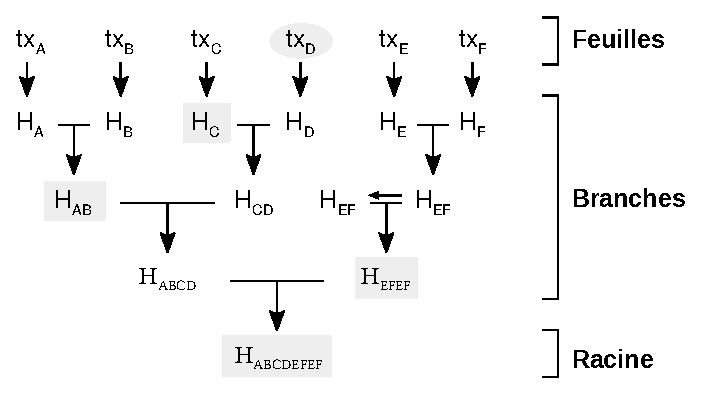
\includegraphics[scale=0.8]{img/merkle-tree.eps}
  \caption{Représentation d'un arbre de Merkle à six feuilles.}
  \label{fig:merkle-tree}
\end{figure}

% Vérification de paiement simplifiée
Cette organisation se révèle particulièrement utile pour les portefeuilles légers (dits à vérification de paiement simplifiée ou SPV) qui ne conservent pas la chaîne de blocs entière mais uniquement la chaîne des entêtes, qui est bien moins volumineuse (un peu plus de \textcolor{darkgray}{62 Mio en novembre 2023}). En effet, pour s'assurer de la présence d'une transaction dans un bloc, ils peuvent se contenter de demander les informations liées à la branche (chemin de Merkle) et procéder aux hachages eux-mêmes\sendnote{Démontrer qu'une feuille fait partie d'un arbre de Merkle requiert de calculer un nombre d'empreintes proportionnel au logarithme binaire du nombre de feuilles ($\log_{2}(n)$), et non pas proportionnel au nombre de feuilles $n$. Pour un bloc de 3000 transactions (moyenne haute sur BTC), cela représente 12 empreintes de 32 octets à obtenir et 12 hachages à effectuer.}. Par exemple, un utilisateur voulant vérifier la confirmation de la transaction $\mathrm{tx}_D$ doit simplement demander les informations $H_C$, $H_{A\!B}$ et $H_{E\!F\!E\!F}$ aux nœuds du réseau et procéder aux différents hachages pour comparer la racine obtenue avec celle contenue dans l'entête. Cela a pour effet de réduire considérablement la charge des portefeuilles légers.

% Racine de Merkle supplémentaire
Depuis l'activation de SegWit le 24 août 2017, chaque bloc contient un arbre de Merkle supplémentaire, subordonné à l'arbre classique des transactions décrit plus haut. Il s'agit de l'arbre témoin qui est l'arbre des transactions intégrant les signatures des transactions SegWit (séparées des transactions classiques). La racine de l'arbre témoin est placée dans la transaction de récompense, de sorte qu'elle est prise en compte dans la racine de Merkle principale, ce qui garantit l'intégrité de l'ensemble.

% --- Horodatage ---

\textbf{L'horodatage.} L'horodatage indique la date et l'heure de construction du bloc qui sont déclarées par le mineur. D'un point de vue technique, il est donné par l'heure Unix, c'est-à-dire le nombre de secondes écoulées depuis le 1\ier{} janvier 1970 \wtime{00:00:00 UTC}. Pour notre bloc, l'horodatage est de $1661407005$ ce qui correspond à la date du 25 août 2022 à 5 heures 56 minutes et 45 secondes (UTC).

Le mineur ne peut pas choisir cet horodatage au hasard. L'heure déclarée doit se situer dans le futur par rapport au temps médian passé (MTP) -- la médiane des horodatages des 11 derniers blocs, qui retarde généralement d'une heure sur le temps réel -- et ne doit pas dépasser l'horloge des nœuds récepteurs de deux heures\pagenote{«~ne doit pas dépasser l'horloge des nœuds récepteurs de deux heures~»~: \url{https://github.com/bitcoin/bitcoin/blob/24.x/src/validation.cpp\#L3483-L3490}.}. Cette contrainte relativement permissive permet au temps réseau de rester relativement cohérent avec la réalité.

% --- Valeur cible ---

\textbf{La valeur cible.} La valeur cible est la valeur minimale que l'identifiant du bloc peut prendre pour que ce bloc constitue une preuve de travail. Plus cette valeur cible est petite, plus il est facile de trouver une solution et de miner un bloc. Elle est déterminée par le réseau selon les règles de l'algorithme d'ajustement de la difficulté.

La valeur cible est encodée comme un nombre flottant où le premier octet représente un exposant particulier et où la mantisse est déterminée par les 3 octets suivants. Ici, elle est égale à $\mathtt{0x09ed88} \times 256^{(\mathtt{0x17} - 3)}$ c'est-à-dire~:

\begin{Verbatim}[fontsize=\footnotesize]
00000000000000000009ed880000000000000000000000000000000000000000
\end{Verbatim}

Cette information donne aussi la difficulté de minage du bloc, qui est inversement proportionnelle à la valeur cible. Il s'agit du quotient de la valeur cible maximale du système par la valeur cible du réseau\sendnote{En notant $c$ la valeur cible, la difficulté est définie par~: \[ d = \frac{C_{\mathrm{max}}}{c} \] où $C_{\mathrm{max}} = \mathtt{0x00ffff} \times 256^{26}$ est la valeur cible maximale du réseau.}. La difficulté minimale du protocole est donc de 1 et celle de notre bloc (arrondie à l'unité près) est quant à elle de $28~351~606~743~494$, ce qui représente un différentiel énorme~! Elle donne également la quantité de travail du bloc, qui est le nombre moyen de hachages nécessaires pour tomber sur une solution\sendnote{En termes mathématiques, le travail d'un bloc est le quotient du nombre d'empreintes possibles par le nombre d'empreintes satisfaisant le problème. En notant $c$ la valeur cible, le travail est~: \[ T = \frac{2^{256}}{c + 1} ~.\]}.

% --- Nonce ---

\textbf{Le nonce.} Le nonce désigne le nombre que le mineur fait varier pour produire la preuve de travail. Ce mot provient de l'expression anglaise «~\eng{for the nonce}~» signifiant «~pour la circonstance, pour l'occasion~», ce qui indique la spécificité de son rôle\sendnote{Une étymologie populaire prétend qu'il serait une contraction de l'expression «~\eng{number used once}~», mais celle-ci est incorrecte.}. Le mineur fait également varier un nonce supplémentaire au sein de la transaction de récompense, le champ du nonce étant trop petit (8 octets) pour la difficulté de minage actuelle. Le nonce de notre bloc est $4~224~551~499$.

Ces deux derniers paramètres (valeur cible et nonce) sont relatifs à la preuve de travail et interviennent dans la formulation du problème mathématique résolu par le mineur. Ce problème se présente sous la forme d'une inégalité mathématique. En notant $c$ la valeur cible du réseau et $\mathrm{EB}$ l'entête du bloc, il s'agit de trouver un nonce $n$ tel que~:

{ \small
\[
\mathrm{SHA256d} ( \ \mathrm{EB} ( \ n \ ) \ ) ~ \le ~ c
\]
}

Comme on l'a dit, le résultat est utilisé comme identifiant du bloc. La preuve de travail est facilement vérifiable~: chaque membre du réseau peut, à partir des données du bloc, s'assurer que le mineur a bien trouvé une solution valide. Dans notre cas, si on compare l'identifiant et la valeur cible, on obtient bien un résultat qui satisfait l'inégalité exigée~:

{ \footnotesize
\begin{align*}
\mathtt{0x000000000000000000065aebf106c8824f4b565d54d6d6df32498b2b041cfd07} & \le \\ \mathtt{0x00000000000000000009ed880000000000000000000000000000000000000000} & ~
\end{align*}
}

\begin{figure}[h]
  \centering
  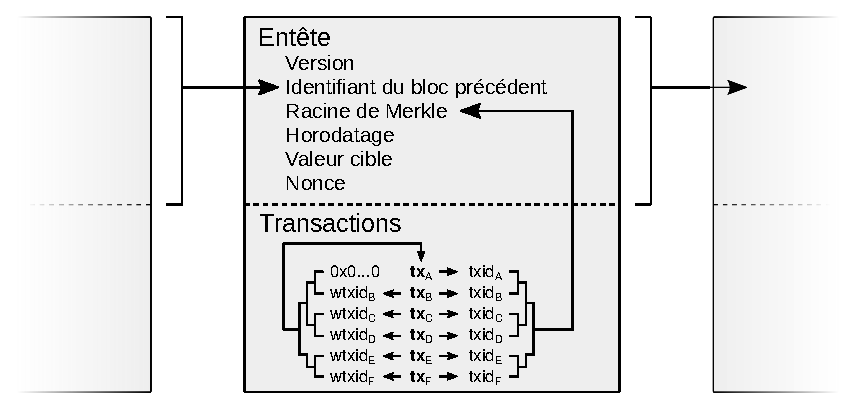
\includegraphics[scale=0.75]{img/bitcoin-segwit-block.eps}
  \caption{Schéma d'un bloc de Bitcoin (avec SegWit).}
  \label{fig:bitcoin-segwit-block}
\end{figure}

\section*{Le revenu du minage} % Le minage, un procédé économique
\addcontentsline{toc}{section}{Le revenu du minage}

% --- Présentation du minage ---

L'une des innovations de Bitcoin est de récompenser la confirmation des transactions à l'aide de son unité de compte interne. Cette propriété crée une incitation économique poussant les mineurs à bien se comporter, ce qui contribue à la solidité du système.

La récompense liée à l'ajout d'un bloc à la chaîne provient en partie de la création monétaire du protocole, d'où le nom de minage employé pour désigner cette activité. Le procédé est en effet analogue à l'extraction minière de l'or dans le monde réel~: les mineurs déploient du capital et dépensent de l'énergie pour obtenir les nouveaux bitcoins. Comme expliqué par Satoshi dans le livre blanc~:

\begin{quote}
«~L'ajout régulier d'une quantité constante de nouvelles pièces est analogue aux mineurs d'or qui dépensent des ressources pour ajouter de l'or à la circulation.\sendnote{Satoshi Nakamoto, \eng{Bitcoin: A Peer-to-Peer Electronic Cash System}, 31 octobre 2008.}~»
\end{quote}

La deuxième partie de la récompense provient des frais de transaction payés par les utilisateurs, qui sont collectés sur les transactions incluses dans le bloc. Le tout est reversé au mineur lorsque le bloc est vérifié et accepté par le réseau. % Le tout est reversé au mineurs lors de la publication d'un bloc valide accepté par le réseau.

% Définition du minage
Le minage est ainsi l'activité économique consistant à rassembler les transactions au sein d'un bloc, à produire la preuve de travail et à diffuser le résultat sur le réseau. Ici, nous le distinguons ainsi du simple hachage, qui consiste juste à réaliser les calculs pour créer la preuve de travail et qui peut être réalisé indépendamment de la sélection de transactions, notamment au sein des coopératives de minage (\eng{mining pools}). Dans ce cadre, les mineurs sont les personnes ou les groupes de personnes réalisant l'activité complète, et les entités se contentant de mettre en place des machines et de déléguer leur pouvoir sur la sélection des transactions ne sont que des «~hacheurs~».

% L'entité réalisant cette activité est appelée un mineur\sendnote{Le terme de mineur peut également parfois désigner la machine utilisée pour produire la preuve de travail.}.

% Déroulement du minage d'un bloc
Le minage se déroule de manière cyclique. Tout d'abord, le mineur sélectionne des transactions à partir de la réserve des transactions (appelée \eng{mempool}) de son nœud. Puis, il construit un bloc candidat en imposant un entête, en assemblant les transactions et en prenant soin de construire une transaction de récompense qui le rémunère. Il fait ensuite varier le nonce et d'autres éléments du bloc candidat afin de produire la preuve de travail. Enfin, dans le cas où il trouve une solution, il diffuse le bloc sur le réseau le plus rapidement possible pour que les autres nœuds le vérifient et l'acceptent comme le nouveau bloc de la chaîne. Dans le cas contraire, si un nouveau bloc est trouvé entretemps, le mineur l'accepte et abandonne son bloc candidat. Dans les deux cas, la procédure reprend du début avec des transactions différentes.

% Transaction de récompense (coinbase)
La récompense de minage est ainsi récupérée par le mineur \emph{via} l'inclusion d'une transaction de récompense au sein du bloc. Celle-ci doit être, par convention, la première transaction du bloc. Elle possède une entrée unique spécifique ne faisant référence à aucune transaction existante. La transaction de récompense est aussi appelée la base de pièce ou \eng{coinbase}, car c'est à partir d'elle que sont formés les nouveaux bitcoins. Le mineur dirige cette transaction vers une adresse qu'il contrôle, de sorte qu'il est récompensé si et seulement si son bloc est valide aux yeux du réseau.

La récompense que le mineur peut se verser doit être inférieure à la somme de la création monétaire et des frais de transaction. Le mineur peut ainsi se rémunérer moins que ce qui est prévu par le protocole, même si cela n'a aucun sens économique direct\sendnote{En décembre 2017, le mineur du bloc 501~726 s'est ainsi rémunéré de la coquette somme de 0~BTC~!}.

% --- Création monétaire ---

La création monétaire se fait intégralement par le biais de la transaction de récompense. Tous les bitcoins dans le système sont ainsi le résultat d'une série de transferts commençant par une telle transaction.

% La particularité de Bitcoin par rapport à ses prédécesseurs, et notamment le système RPOW, est d'offrir une politique monétaire fixe malgré un recours à la preuve de travail. Cette caractéristique permet d'éviter la création monétaire liée à l'innovation technique, qui est exponentielle comme l'illustre la loi de Moore.

% Ajustement de la difficulté
La particularité de cette création monétaire est qu'elle est fixée dans le temps et qu'elle n'est pas proportionnelle à la puissance de calcul déployée. Cela est rendu possible par l'algorithme d'ajustement de la difficulté, qui dérive du fait que le système constitue un serveur d'horodatage distribué. En effet, les blocs étant horodatés, il est possible de mesurer leur rythme de production passé et d'ajuster la difficulté de minage en conséquence. Ainsi, comme l'écrivait Satoshi~:

\begin{quote}
«~Afin de compenser l'augmentation de la vitesse du matériel et la variation de l'intérêt des nœuds actifs au fil du temps, la difficulté de la preuve de travail est déterminée par une moyenne mobile visant un nombre moyen de blocs par heure. Si ces blocs sont générés trop rapidement, la difficulté augmente.\sendnote{Satoshi Nakamoto, \eng{Bitcoin: A Peer-to-Peer Electronic Cash System}, 31 octobre 2008.}~»
\end{quote}

Dans la version principale de Bitcoin, l'intervalle de temps entre chaque bloc (temps de bloc) visé est de 10 minutes ou 600 secondes. L'ajustement a lieu tous les 2016 blocs, ce qui correspond environ à deux semaines, selon la moyenne simple du temps de bloc sur cette période. La nouvelle valeur cible est calculée\sendnote{Dans Bitcoin Core, l'algorithme d'ajustement est décrit par la fonction \longstring{CalculateNextWorkRequired} dans le fichier \texttt{pow.cpp}. La variation est limitée à un facteur 4 (multiplication comme division) pour éviter les instabilités. L'algorithme \emph{surestime} la puissance de calcul déployée car le temps écoulé est mesuré sur 2015 intervalles, et non pas 2016 comme cela devrait se faire.}\pagenote{«~la fonction CalculateNextWorkRequired dans le fichier pow.cpp~»~: \url{https://github.com/bitcoin/bitcoin/blob/24.x/src/pow.cpp\#L49-L72}.} à partir de la valeur cible précédente ($c_{k-1}$) et du temps écoulé depuis le dernier ajustement ($t_{k-1}$)~:

{ \small
\[
c_{k} = \frac{c_{k-1} \cdot t_{k-1}}{2016 \cdot 600}
\]
}

% Politique monétaire
Grâce à cet ajustement, le bitcoin possède une politique monétaire déterminée, qui n'est pas soumise à l'arbitraire direct d'un tiers de confiance ou à la quantité de capital déployé. Cette caractéristique le différencie de la monnaie fiat (comme le dollar) qui est émise de manière discrétionnaire par une banque centrale, ou du métal précieux (comme l'or) dont la quantité extraite connaît ses propres variations et suit la demande du marché à long terme. Cette politique monétaire a été décrite précisément pour la première fois par Satoshi Nakamoto dans son courriel de lancement du 8 janvier 2009 où il écrivait~:

\begin{quote}
«~La quantité en circulation totale sera de 21~000~000 pièces. Elle sera distribuée aux nœuds du réseau lorsqu'ils créeront des blocs, le montant étant divisé par deux tous les 4 ans.

les quatre premières années : 10~500~000 pièces\\
les quatre années suivantes : 5~250~000 pièces\\
les quatre années suivantes : 2~625~000 pièces\\
les quatre années suivantes : 1~312~500 pièces\\
etc...

Lorsque cela est épuisé, le système peut prendre en charge les frais de transaction si nécessaire. Il est basé sur la concurrence du marché ouvert, et il y aura probablement toujours des nœuds prêts à traiter les transactions gratuitement.\sendnote{Satoshi Nakamoto, \eng{Bitcoin v0.1 released}, \wtime{08/01/2009 19:27:40 UTC}~: \url{https://www.metzdowd.com/pipermail/cryptography/2009-January/014994.html}.}~»
\end{quote}

Elle est bien évidemment inscrite dans le code\pagenote{«~Elle est bien évidemment inscrite dans le code~»~: \url{https://github.com/bitcoin/bitcoin/blob/24.x/src/validation.cpp\#L1473-L1484}}, où elle est appelée subvention ou \eng{subsidy} en anglais.

% Réduction de moitié
L'originalité principale de cette politique monétaire est que la création monétaire est réduite de moitié de manière brusque tous les 210~000 blocs (soit environ 4 ans) lors de ce qu'on appelle couramment un \eng{halving}. \textcolor{darkgray}{En 2023}, trois réductions de moitié avaient déjà eu lieu sur le réseau Bitcoin principal~: la première s'est produite le 28 novembre 2012, lorsque la subvention du protocole est passée de 50 bitcoins par bloc à 25~; la deuxième le 9 juillet 2016, avec une baisse à 12,5 bitcoins par bloc~; la troisième le 11 mai 2020, où la subvention a été réduite à 6,25 bitcoins par bloc.  \textcolor{darkgray}{La prochaine réduction de moitié devrait se passer en 2024, lors de laquelle les nouveaux bitcoin émis seront de 3,125 par bloc.} Sauf modification des règles de consensus, la dernière réduction de moitié sera la 33\ieme{} et aura lieu aux alentours de 2140. En effet, le montant de création monétaire par bloc passera alors en dessous du satoshi, soit zéro par troncature à l'unité.

% old function:
%
% \begin{Verbatim}[fontsize=\small]
% int64 CBlock::GetBlockValue(int64 nFees) const
% {
%     int64 nSubsidy = 50 * COIN;
% 
%     // Subsidy is cut in half every 4 years
%     nSubsidy >>= (nBestHeight / 210000);
% 
%     return nSubsidy + nFees;
% }
% \end{Verbatim}


% Limite des 21 millions
À long terme, cette politique monétaire atypique fait du bitcoin une monnaie à quantité fixe. En effet, le montant maximal de bitcoins en circulation doit tendre, au fil du temps, vers une limite~: la fameuse limite des 21 millions. Celle-ci n'est qu'une déduction des conditions d'émission susmentionnées, ce qui s'exprime en termes mathématiques par la convergence de la série des montants minés entre les halvings\sendnote{Cette convergence est illustrée par le paradoxe d'Achille et de la tortue formulé par le philosophe grec Zénon. La suite $\left( \sum_{i=1}^{n} (1/2)^i \right)$ converge vers $1$ lorsque $n\to+\infty$.}~:

{ \small
\[
N_{\mathrm{max}} = \sum_{i=0}^{+\infty} \left( {210~000 \cdot \frac{50}{2^i}} \right) = 21~000~000 \cdot \sum_{i=1}^{+\infty} \left(\frac{1}{2}\right)^i = 21~000~000
\]
}

% Limite jamais atteinte
La limite des 21 millions est une borne supérieure~: en l'absence d'un changement des règles de consensus, elle ne sera jamais formellement atteinte, en raison de la nature optionnelle de la récompense de minage, du caractère discret des unités et de la perte irrémédiable de bitcoins. De plus, les bitcoins dont les propriétaires ont perdu leurs clés privées réduisent considérablement la quantité réelle de bitcoins en circulation sans pour autant que cela ne soit pris en compte dans le calcul.

% Remplacement par les frais
La création monétaire a ainsi vocation à s'amenuiser et à devenir négligeable, et ce plus rapidement que l'on imagine. En effet, \textcolor{darkgray}{en 2023, le nombre de bitcoins dépensables avait déjà dépassé les 19,5 millions.} C'est pourquoi cette subvention doit en toute logique être remplacée par l'autre source de revenu pour les mineurs, à savoir les frais de transaction\sendnote{«~Une fois qu'un nombre prédéterminé de pièces a été mis en circulation, l'incitation peut être entièrement financée par les frais de transaction et ne plus requérir aucune inflation.~» -- Satoshi Nakamoto, \eng{Bitcoin: A Peer-to-Peer Electronic Cash System}, 24 mars 2009.}.

% Frais de transaction
Les frais de transaction sont les commissions payées par les utilisateurs pour la confirmation de leurs transactions. Les frais d'une transaction peuvent être versés directement par l'expéditeur (client) ou indirectement par le destinataire (commerçant) par l'intermédiaire d'une remise sur le produit vendu. Ils sont récupérés par le mineur sur chaque transaction du bloc selon une règle implicite~: il s'agit de la différence entre le montant en entrée de la transaction et son montant en sortie. Cette différence peut être de zéro (transaction gratuite), mais elle est toujours comptabilisée. Les frais sont ajoutés à la transaction de récompense indistinctement des bitcoins issus de la création monétaire. Bitcoin intègre ainsi un système interne et optimisé de frais de transaction, qui évite l'alourdissement inutile des transactions et des blocs.

% Existence des frais
L'existence des frais de transaction a vocation à perdurer par conception, même si ceux-ci devenaient très bas. Contrairement à l'opinion exprimée par Satoshi, la confirmation d'une transaction a en général un coût, même marginal\sendnote{Le seul cas envisageable de transaction gratuite est celui d'une grande transaction de consolidation qui amoindrirait la charge des mineurs en réduisant considérablement l'ensemble des UTXO.}, et une transaction qui paie trop peu de frais par rapport à la charge apportée n'a aucune raison économique d'être confirmée. De ce fait, il n'y a pas lieu de s'imaginer que la chaîne de blocs s'arrête.

% Limite de capacité transactionnelle
En outre, les règles du protocole restreignent usuellement l'espace de bloc par le biais d'une limite explicite sur la taille (ou le poids) des blocs. Cette restriction crée un plafond de production qui, lorsqu'il est atteint, fait que le mineur rationnel sélectionne les transactions qui paient le taux le plus élevé de frais, toutes choses étant égales par ailleurs. Il existe donc, dans le cas d'une congestion du réseau, un effet d'enchères pouvant faire augmenter le niveau moyen des frais de manière drastique.

% --- Alternatives aux frais ---

Bien que les frais constituent la façon principalement envisagée de rémunérer les mineurs à terme, des méthodes alternatives de financement ont été proposées.

% Émission de queue
La première est l'émission de queue (\eng{tail emission}), qui consiste à maintenir une création monétaire constante au cours du temps, dans le but que le revenu de minage ne tombe pas trop bas\sendnote{Peter Todd, \eng{Surprisingly, Tail Emission Is Not Inflationary}, 9 juillet 2022~: \url{https://petertodd.org/2022/surprisingly-tail-emission-is-not-inflationary}.}. L'instauration de cette caractéristique aurait pour effet de modifier la politique monétaire du bitcoin et de faire disparaître la limite des 21 millions, d'où son caractère hautement controversé.

Pour donner un exemple, l'émission de queue est mise en place dans la variante Monero depuis 2015. Elle est devenue effective le 9 juin 2022, date depuis laquelle il se crée 0,3~monero par minute, soit un taux de création monétaire annualisé de 0,87~\% \textcolor{darkgray}{à ce moment-là}. Une telle émission de queue existe également dans Dogecoin depuis 2015, à raison de 10~000 dogecoins par minute, pour un taux annualisé de 3,8~\% \textcolor{darkgray}{en décembre 2022}.

% Demeurage
La deuxième méthode de financement proposée est le demeurage, ou coût de détention, qui consiste à prélever la monnaie demeurée immobile depuis un temps donné\sendnote{Jorge Timón, \eng{Freicoin: bitcoin with demurrage}, \wtime{24/02/2011 11:56:03 UTC}~: \url{https://bitcointalk.org/index.php?topic=3816.msg54170\#msg54170}.}. Les bitcoins de Satoshi, qui représentent une manne financière importante, sont notamment concernés. Toutefois, il s'agirait d'une atteinte au système de propriété de Bitcoin et il y a donc peu de chances que cette méthode rencontre le succès.

\section*{La chaîne la plus longue}
\addcontentsline{toc}{section}{La chaîne la plus longue}

Venons-en maintenant au sujet central de ce chapitre~: l'atteinte du consensus par le minage. Comme nous l'avons expliqué ci-dessus, le minage est le procédé permettant aux mineurs d'ajouter des blocs à la chaîne, chose pour laquelle ils sont rémunérés. Mais nous n'avons pas exposé comment il permettait d'arriver à un accord dans un contexte antagoniste, en présence d'acteurs malveillants «~byzantins~».

% Communication
Les nœuds suivent un protocole composé des règles de réseau, qui leur permettent de rentrer en communication, et des règles de consensus, qui concernent la forme des transactions et des blocs, que nous détaillerons dans le chapitre ~\ref{ch:changement}. Les nœuds qui enfreignent ces règles voient leurs connexions être fermées par leurs pairs et sont mis sur liste noire si nécessaire. Il est donc impossible de faire accepter une transaction ou un bloc au réseau qui ne soit valide selon les règles de consensus.

Néanmoins, les nœuds byzantins peuvent semer la discorde dans le respect des règles de consensus, en produisant des blocs concurrents. En effet, rien n'empêche \emph{a priori} un attaquant de produire des blocs de transactions qui soient valides mais qui ne soient pas rattachés à la branche principale et de les soumettre au réseau.

% --- Principe de la chaîne la plus longue ---

Ce problème est résolu par le biais d'un principe simple mais efficace~: le principe de la chaîne la plus longue. Celui-ci a été décrit par Satoshi dans le livre blanc~: 

\begin{quote}
«~La décision majoritaire est représentée par la chaîne la plus longue, sur laquelle le plus grand effort de preuve de travail a été investi.\sendnote{Satoshi Nakamoto, \eng{Bitcoin: A Peer-to-Peer Electronic Cash System}, 31 octobre 2008.}~»
\end{quote}

Les nœuds du réseau se mettent d'accord en sélectionnant la chaîne possédant le plus de travail accumulé\pagenote{«~la chaîne possédant le plus de travail accumulé~»~: Ce principe a été redéfini le 25 juillet 2010 au sein de la version 0.3.3 du logiciel~: \url{https://github.com/bitcoin/bitcoin/commit/3b7cd5d89a226426df9c723d1f9ddfe08b7d1def}.}, ce qui se matérialise généralement par une chaîne plus longue en nombre de blocs\sendnote{En réalité, au début c'était bel et bien la chaîne possédant le plus de blocs qui était sélectionnée. Mais ce principe a été redéfini le 25 juillet 2010 au sein de la version 0.3.3 du logiciel pour prendre en compte la notion de travail.}. Lorsqu'une chaîne possédant une quantité strictement plus grande de travail est publiée, les nœuds suivent cette chaîne, que celle-ci soit dans la continuité de la dernière ou qu'elle fasse référence à une branche plus ancienne. Cette règle fait en sorte que les nœuds suivent toujours la chaîne sur laquelle un montant supérieur d'énergie a été investi. L'algorithme de consensus résultant de l'application de ce principe est appelé l'algorithme de consensus de Nakamoto par preuve de travail, en hommage à son concepteur.

% --- Embranchement ---

La meilleure manière d'appréhender le fonctionnement de cet algorithme est de prendre le cas d'un embranchement (ou \eng{fork} en anglais) de la chaîne. Celui-ci peut être créé par un acteur malveillant, mais dans la réalité il est généralement engendré de manière accidentelle, lorsque deux mineurs éloignés trouvent chacun un bloc différent dans un intervalle de temps réduit et que les nœuds du réseau ne reçoivent pas le même bloc en premier. Il n'y a alors aucun moyen de départager les deux branches, celles-ci étant également correctes en vertu du principe de la chaîne la plus longue. Ce type d'embranchement accidentel est commun et se produit de temps en temps sur le réseau pour des raisons de latence.

Cette situation et sa résolution ont été décrites par Satoshi dans le livre blanc~:

\begin{quote}
«~Si deux nœuds transmettent simultanément des versions différentes du bloc suivant, certains nœuds peuvent recevoir l'une ou l'autre version en premier. Dans ce cas, ils travaillent sur la première version qu'ils ont reçue, mais conservent l'autre branche au cas où elle deviendrait plus longue. L'égalité est rompue lorsque la preuve de travail suivante est trouvée et qu'une branche devient plus longue~; les nœuds qui travaillaient sur l'autre branche passent alors sur la chaîne la plus longue.\sendnote{Satoshi Nakamoto, \eng{Bitcoin: A Peer-to-Peer Electronic Cash System}, 31 octobre 2008.}~»
\end{quote}

Le réseau passe par trois étapes. Tout d'abord, il se comporte de manière attendue~: les mineurs prolongent la chaîne la plus longue, sur laquelle le reste des nœuds se coordonnent. Puis, le conflit a lieu~: deux branches correctes coexistent et les mineurs travaillent pour prolonger la chaîne à partir du bloc reçu en premier. Enfin, l'embranchement est résolu~: un mineur trouve un nouveau bloc et sa chaîne, qui devient plus longue, est acceptée par le réseau.

Il se produit alors ce qu'on appelle une recoordination (\eng{reorganization}) qui réconcilie les nœuds du réseau entre eux. Le bloc de la branche faible est considéré comme incorrect et mis de côté. On dit que ce bloc est rendu orphelin (\eng{orphaned}) car il perd son attachement à la chaîne mère\sendnote{L'appellation (quelque peu ambigüe) de «~bloc orphelin~» a été introduite par Satoshi Nakamoto au sein de la première version du logiciel. On parle aussi de «~bloc oncle~» (en référence au fait qu'il ne donne pas de descendance fertile) ou bien de «~bloc périmé~» (\eng{stale block}).}. La branche forte (possédant le plus de travail accumulé) est considérée comme la version correcte de la chaîne.

\begin{figure}[h]
  \centering
  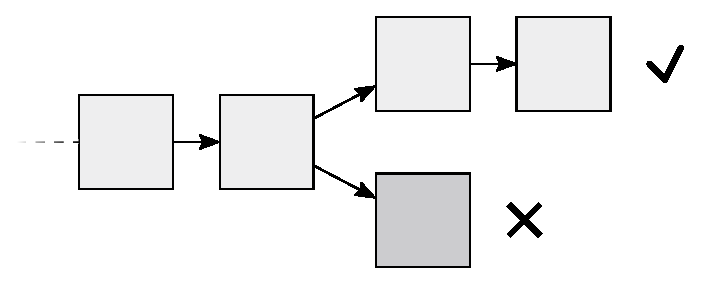
\includegraphics[scale=0.8]{img/blockchain-common-fork.eps}
  \caption{Schéma d'un embranchement commun de la chaîne.}
  \label{fig:blockchain-common-fork}
\end{figure}

Tout conflit sur le réseau est résolu de la sorte, ce qui a pour conséquence de conférer une nature particulière à l'algorithme de Nakamoto, et par extension à Bitcoin.

% Tout conflit sur le consensus est résolu de la sorte. Le fonctionnement de l'algorithme de Nakamoto possède des conséquences sur la nature de Bitcoin.

% --- Deux contraintes sécuritaires ---

% Honnêteté de la majorité
Ce fonctionnement impose tout d'abord deux contraintes majeures sur la sécurité. La première est que la sécurité minière du réseau repose sur la supposition qu'une majorité de la puissance de calcul («~51~\%~») se comporte de manière honnête. Comme l'expliquait Satoshi~:

\begin{quote}
«~Le système est sécurisé tant que les nœuds honnêtes contrôlent collectivement plus de puissance de calcul qu'un groupe de nœuds qui coopéreraient pour réaliser une attaque.\sendnote{Satoshi Nakamoto, \eng{Bitcoin: A Peer-to-Peer Electronic Cash System}, 31 octobre 2008.}~»
\end{quote}

% Sécurité probabiliste
La seconde est que la sécurité d'une transaction donnée est probabiliste et dépend de la profondeur à laquelle elle se trouve dans la chaîne. La transaction est d'abord vérifiée par le réseau (zéro confirmation), puis confirmée au sein d'un bloc (une confirmation) et finit par être considérée comme irréversible, généralement à partir de six confirmations pour les montants ordinaires sur la version principale de Bitcoin. Cela contraint l'utilisateur à estimer le nombre de confirmations qu'il doit attendre en fonction de la sécurité désirée.

% Période de maturation de la récompense de minage
Cette particularité se transcrit dans le fonctionnement du minage par la maturité de la base de pièce (\eng{coinbase maturity}), qui est le nombre de confirmations nécessaire pour que la sortie de la transaction de récompense devienne dépensable. Cette contrainte est mise en place pour éviter la mauvaise utilisation des fonds due à une recoordination peu profonde. Le délai sur le réseau BTC est aujourd'hui de 101 confirmations\pagenote{«~Le délai sur le réseau BTC est aujourd'hui de 101 confirmations~»~: \url{https://github.com/bitcoin/bitcoin/blob/23.x/src/consensus/consensus.h\#L18-L19}}.

% --- Trois avantages ---

% Objectivité
L'algorithme de Nakamoto possède également trois avantages principaux. D'abord, il a pour intérêt d'avoir un critère objectif sur lequel se reposer~: tout le monde peut reconstituer la chaîne à partir du bloc de genèse et constater qu'il s'agit de la chaîne correcte. Même dans le cas extrême d'un cloisonnement mondial et prolongé du réseau dû à une guerre ou une catastrophe naturelle, le système peut finir par se recoordonner\sendnote{Satoshi Nakamoto, \eng{Re: Anonymity}, \wtime{08/07/2010, 19:12:00 UTC}~: \url{https://bitcointalk.org/index.php?topic=241.msg2071\#msg2071}.}.

% Ouverture
Ensuite, il permet la participation ouverte au consensus~: tout ce qui est requis du mineur est une preuve de travail valide, de sorte que le minage est anonyme par essence.

% Robustesse
Enfin, cet algorithme par preuve de travail assure la robustesse du réseau~: un mineur n'a pas à connaître tous les autres participants, ce qui permet au réseau d'être composé de dizaines (voire de centaines) de milliers de nœuds.

\section*{La résistance à la double dépense}
\addcontentsline{toc}{section}{La résistance à la double dépense}

La double dépense est le fait pour un acteur de faire accepter successivement deux transactions au réseau dans le but de déstabiliser l'état du système et d'en bénéficier d'une manière ou d'une autre. La deuxième transaction peut constituer une annulation de la première, dans laquelle l'acteur malveillant réalise un transfert vers lui-même.

% Transactions non confirmées
La double dépense constitue un problème dans le cas des transactions non confirmées, c'est-à-dire des transactions qui ont été diffusées sur le réseau, vérifiées par les nœuds et placées dans leurs \eng{mempools}, mais qui n'ont pas encore été incluses dans un bloc de la chaîne. Aucun consensus n'a été réalisé à propos de ces transactions, mais le commerçant peut décider de les accepter dans le cas où les montants engagés sont faibles\sendnote{Dans un message sur le forum en juillet 2010, Satoshi écrivait à propos de l'acceptation des transactions non confirmées~:
\begin{quote}
\footnotesize «~Je pense qu'il sera possible pour une entreprise de traitement des paiements de fournir comme service la distribution rapide de transactions avec une vérification suffisante en 10 secondes ou moins.

Les nœuds du réseau n'acceptent que la première version d'une transaction qu'ils reçoivent pour l'incorporer dans le bloc qu'ils essaient de générer. Lorsqu'on diffuse une transaction et que quelqu'un d'autre diffuse une double dépense au même moment, c'est une course à la propagation vers le plus grand nombre de nœuds qui a lieu. Si l'un d'elles a une légère avance, elle se propagera géométriquement dans le réseau plus rapidement et atteindra la plupart des nœuds. [...]

Le processeur de paiement a des connexions avec de nombreux nœuds. Lorsqu'il reçoit une transaction, il l'envoie et, en même temps, surveille le réseau pour détecter les doubles dépenses. S'il reçoit une double dépense sur l'un de ses nombreux nœuds d'écoute, il signale que la transaction est mauvaise.~»
\end{quote}
Satoshi Nakamoto, \eng{Re: Bitcoin snack machine (fast transaction problem)}, \wtime{17/07/2010 22:29:13 UTC}~: \url{https://bitcointalk.org/index.php?topic=423.msg3819\#msg3819}.}. Le risque est qu'un fraudeur reparte avec la marchandise et réussisse à faire accepter une version alternative de la transaction vue par le commerçant, soit en la diffusant au même moment et en espérant qu'elle arrive en premier au mineur, soit en payant plus de frais (ce qui peut être fait systématiquement avec Replace-by-Fee) pour soudoyer le mineur, soit encore en minant préalablement un bloc contenant la transaction (attaque Finney\sendnote{Hal Finney, \eng{Re: Best practice for fast transaction acceptance - how high is the risk?}, \wtime{13/02/2011, 21:48:44 UTC}~: \url{https://bitcointalk.org/index.php?topic=3441.msg48384\#msg48384}.}).

% Solution : le minage
La solution à ce problème est de se mettre d'accord sur la transaction correcte pour faire disparaître la double dépense, \emph{ce qui est précisément le but du minage}. Cependant, le minage n'empêche pas la double dépense de manière absolue, étant plutôt un mécanisme de résistance. Voyons ce qui garantit cette caractéristique.

% --- Attaque de double dépense par recoordination de chaîne ---

Un certain nombre de perturbations opportunistes peuvent avoir lieu au niveau de l'activité minière comme l'attaque vector76\sendnote{vector76, \eng{Re: Fake Bitcoins?}, \wtime{17/08/2011 17:37:56 UTC}~: \url{https://bitcointalk.org/index.php?topic=36788.msg463391\#msg463391}.} ou le minage égoïste\sendnote{Ittay Eyal, Emin Gün Sirer, \eng{Majority is not Enough: Bitcoin Mining is Vulnerable}, 2013.}, mais la plus importante d'entre elles est l'attaque de double dépense par recoordination de chaîne. Celle-ci consiste à utiliser une part importante de la puissance de calcul du réseau (généralement une majorité) afin de réécrire le passé de la chaîne et modifier une ou plusieurs transactions. Cette attaque a été décrite précisément par Satoshi Nakamoto dans le livre blanc\sendnote{«~Nous considérons le scénario d'un attaquant qui tente de générer une chaîne alternative plus rapidement que la chaîne honnête. Même en cas de réussite, cela n'expose pas le système à des modifications arbitraires [...]. Un attaquant peut seulement essayer de modifier l'une de ses propres transactions afin de récupérer l'argent qu'il a récemment dépensé.~» -- Satoshi Nakamoto, \eng{Bitcoin: A Peer-to-Peer Electronic Cash System}, 31 octobre 2008.} et dans son courriel de réponse à John Levine du 3 novembre 2008\sendnote{«~Même si un individu malintentionné parvenait à maîtriser le réseau, ce n'est pas comme s'il devenait instantanément riche. Tout ce qu'il pourrait faire, c'est récupérer l'argent qu'il a lui-même dépensé, comme un chèque sans provision. Pour l'exploiter, il faudrait qu'il achète une chose à un commerçant, qu'il attende qu'elle soit expédiée, puis qu'il prenne le contrôle du réseau et essaie de récupérer son argent. Je ne pense pas qu'il puisse se faire autant d'argent en essayant de monter un tel stratagème qu'en générant des bitcoins. Avec une ferme de machines zombies aussi grande, il pourrait générer plus de bitcoins que tous les autres réunis.~» (Satoshi Nakamoto, \eng{Re: Bitcoin P2P e-cash paper}, \wtime{03/11/2008 16:23:49}~: \url{https://www.metzdowd.com/pipermail/cryptography/2008-November/014818.html})}. % "Even if a bad guy does overpower the network, it's not like he's instantly rich.  All he can accomplish is to take back money he himself spent, like bouncing a check.  To exploit it, he would have to buy something from a merchant, wait till it ships, then overpower the network and try to take his money back.  I don't think he could make as much money trying to pull a carding scheme like that as he could by generating bitcoins.  With a zombie farm that big, he could generate more bitcoins than everyone else combined."

% Majorité de la puissance de calcul
Cette attaque est réalisée en trois étapes. Elle peut être faite à l'aide d'une minorité de la puissance de calcul, auquel cas elle ne possède qu'une certaine probabilité de réussir. Cependant, par souci de simplicité, nous supposerons qu'un mineur a réuni la majorité de la puissance de calcul du réseau. L'attaque constitue donc une attaque des 51~\%, aussi appelée attaque de la majorité.

% Achat d'un bien
La première étape est l'achat d'un bien ou d'un service auprès d'un commerçant. L'attaquant procède à une transaction en bitcoins (dite «~légitime~») en l'échange de quoi le commerçant lui fournit une chose de même valeur. Typiquement, il s'agira d'une autre cryptomonnaie ou du dollar auprès d'une plateforme d'échange.

% Minage d'une chaîne parallèle
La deuxième étape est le minage d'une chaîne parallèle. Une fois que la transaction légitime a été confirmée au sein d'un bloc, l'attaquant construit une chaîne parallèle en secret à partir du bloc précédent, qu'il prend soin de ne pas dévoiler au reste du réseau. Dans le même temps, il crée et signe une autre transaction (dite «~frauduleuse~») qui dépense les mêmes bitcoins que la première et qui les renvoie vers une adresse en son contrôle. Il inclut cette transaction frauduleuse dans sa chaîne parallèle. Puisque l'attaquant dispose de la majorité de la puissance de calcul du réseau, il est sûr qu'à un moment ou à un autre, cette chaîne sera plus longue que l'autre.

% Recoordination
La troisième étape est la recoordination de chaîne, représentée sur la figure~\ref{fig:doublespending-attack}. L'attaquant a continué de miner sa chaîne parallèle jusqu'à la livraison du bien économique acheté. À ce moment-là, il dévoile sa chaîne au reste du réseau, qui doit accepter celle-ci en vertu du principe de la chaîne la plus longue. Les nœuds procèdent alors à une recoordination~: les blocs de l'ancienne chaîne sont écartés (rendus orphelins), leurs transactions sont remises dans la mempool et les nouveaux blocs sont vérifiés et ajoutés à la chaîne. Comme la transaction légitime dépense les mêmes fonds que la transaction frauduleuse, qui est incluse dans la nouvelle chaîne, cette transaction légitime est invalidée en tant que double dépense. Le commerçant ne possède plus les bitcoins, qui reviennent à l'attaquant.

\begin{figure}[h]
  \centering
  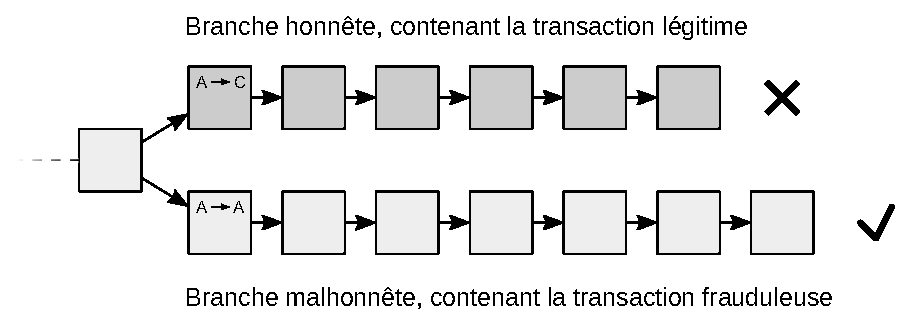
\includegraphics[scale=0.7]{img/mining-attack-doublespending.eps}
  \caption{Attaque de double dépense par recoordination de chaîne.}
  \label{fig:doublespending-attack}
\end{figure}

Il s'agit d'une attaque opportuniste~: elle est motivée par un gain, c'est-à-dire le bien économique obtenu, qui doit être supérieur au coût (matériel, logistique, électrique et logiciel) nécessaire pour y procéder. Sur le réseau Bitcoin principal, ce coût se chiffre aujourd'hui en milliards de dollars\sendnote{Braiins, \eng{How Much Would it Cost to 51\% Attack Bitcoin?}, 11 janvier 2021~: \url{https://braiins.com/blog/how-much-would-it-cost-to-51-attack-bitcoin}.}.

Cette attaque doit être distinguée de la censure, que nous décrirons dans le chapitre~\ref{ch:censure}, et qui consiste à refuser de confirmer des transactions selon un critère arbitraire. Cette dernière repose en effet sur des incitations \emph{extérieures} à l'économie de Bitcoin, le mineur rationnel n'ayant, au sein du système, aucun intérêt économique à ne pas inclure les transactions payant un taux de frais suffisant dans ses blocs.

% --- Incitation ---

Comme souligné par Satoshi, le système est sécurisé tant que la majorité de la puissance de calcul est associée à des nœuds honnêtes, c'est-à-dire des nœuds qui ne cherchent pas à réaliser des doubles dépenses, ni censurer. La sécurité minière repose donc sur une barrière de sécurité, qui représente la charge financière de l'attaquant pour réaliser une double dépense.

% Procédé économique
Cette barrière n'est pas construite de manière bénévole mais repose sur la récompense du protocole, faisant du minage un procédé essentiellement \emph{économique}. En particulier, la résistance à la double dépense -- à savoir la difficulté à effectuer une attaque de double dépense -- dérive directement du revenu minier total, qui incite les nœuds à rester honnêtes. Tel que l'écrivait Satoshi dans le livre blanc~:

\begin{quote}
«~L'incitation peut contribuer à encourager les nœuds à rester honnêtes. Si un attaquant cupide est capable de réunir plus de puissance de calcul que l'ensemble des nœuds honnêtes, il aura à choisir entre l'utiliser pour escroquer des gens en leur récupérant ses paiements, ou l'utiliser pour générer de nouvelles pièces. Il devrait trouver plus rentable de respecter les règles du jeu, celles-ci lui permettant d'obtenir plus de nouvelles pièces que tous les autres réunis, plutôt que de saper le système et la validité de sa propre richesse.\sendnote{Satoshi Nakamoto, \eng{Bitcoin: A Peer-to-Peer Electronic Cash System}, 31 octobre 2008.}~»
\end{quote}

Non seulement la récompense peut être supérieure au gain d'une attaque de double dépense, mais la valeur des bitcoins servant à réaliser la transaction peut aussi être réduite par ladite attaque. En effet, si l'attaque était amenée à être couronnée de succès, on peut imaginer que les différents acteurs diminueraient leur confiance dans le système, arrêteraient de l'utiliser pour le commerce et cèderaient une partie de leur épargne, faisant baisser le revenu de minage et la valeur d'échange du bitcoin. De plus, la spécialisation du matériel de minage (quand elle existe) alourdit le coût de l'attaque, car ce matériel perd dans ce cas en utilité. D'un point de vue purement opportuniste, il est donc la plupart du temps bien plus rentable d'utiliser son capital de manière honnête.

Il est ainsi arrivé que des agrégats de mineurs rassemblent plus de 51~\% de la puissance de calcul, comme la coopérative GHash.io en juillet 2014, sans qu'aucune attaque ne se produise. Et même si une telle attaque avait lieu, celle-ci ne serait pas forcément fatale pour le système à long terme. Comme l'écrivait Satoshi~:

\begin{quote}
«~Même en cas de réussite, cela n'expose pas le système à des modifications arbitraires, comme la création de valeur \emph{ex nihilo} ou l'appropriation d'argent n'ayant jamais appartenu à l'attaquant. Les nœuds ne vont pas accepter une transaction invalide comme paiement, et les nœuds honnêtes n'accepteront jamais un bloc les contenant.\sendnote{Satoshi Nakamoto, \eng{Bitcoin: A Peer-to-Peer Electronic Cash System}, 31 octobre 2008.}~»
\end{quote}

Ainsi de nombreuses attaques de ce type ont déjà eu lieu sur certaines variantes de Bitcoin au fil des années, réduisant leur réputation au passage, mais sans qu'elles ne soient pour autant anéanties. On peut notamment citer Ethereum Classic qui a subi plusieurs recoordinations agressives entre 2019 et 2020\pagenote{«~Ethereum Classic qui a subi plusieurs recoordinations agressives entre 2019 et 2020~»~: Plus précisément~: le 7 janvier 2019, le 31 juillet 2020, le 6 août 2020 et le 29 août 2020.}.

\section*{L'industrie minière}
\addcontentsline{toc}{section}{L'industrie minière}

Le minage est une activité économique à part entière, la récompense de minage servant à rémunérer le service apporté par le mineur. Cette récompense paie pour le coût de l'électricité, de l'infrastructure matérielle et logistique, et de la maintenance logicielle. Elle compense le risque de production de blocs orphelins. Elle rémunère la confirmation des transactions censurées. Et enfin elle récompense la renonciation temporaire à la liquidité (intérêt originaire du prêteur) et le risque économique général (profit de l'entrepreneur).

Du côté de l'infrastructure matérielle, les mineurs ont besoin de déployer un certain nombre d'éléments~: les machines de hachage (systèmes de refroidissement compris) pour procéder aux calculs liés à la preuve de travail, le processeur pour traiter les blocs et vérifier les signatures, la mémoire pour conserver la chaîne (l'historique), l'ensemble des UTXO (l'état) et la réserve des transactions en attente, la bande passante pour envoyer et recevoir les transactions et les blocs,~etc. Et force est de constater que tout cela s'est industrialisé au fur et à mesure des années.

% Oublis (logistique) :
% - l'absolue nécessité de pouvoir se relocaliser;
% - la nécessité de disposer d'installation électrique pointue (voire d'en faire construire, via groupes, transformateurs ou centrales électriques);
% - la main d'oeuvre;
% - l'entretien;
% - la réparation;
% - les ingénieurs derrière la pool;
% - les developpeurs et ingénieurs en lien avec les entreprises énergétiques de la grille électrique (Texas), qui développent des logiciels qui viennent à downclock les machines en fonction des besoins.

% --- Industrialisation ---

L'amélioration de la machine pour procéder au hachage illustre bien cette industrialisation. Initialement les mineurs minaient avec le processeur central (CPU) de leur ordinateur. Puis, en 2010, sous l'impulsion de Laszlo Hanyecz puis d'ArtForz, le minage par processeur graphique (GPU) s'est développé. En 2011, est apparu le premier circuit logique programmable FPGA consacré au minage, qui donnait un meilleur rendement que les cartes graphiques\pagenote{«~En 2011, est apparu le premier circuit logique programmable FPGA consacré au minage~»~: fpgaminer, \eng{Official Open Source FPGA Bitcoin Miner (Spartan-6 Now Tops Performance per \$!)}, \wtime{20/05/2011 02:33:56 UTC}~: \url{https://bitcointalk.org/index.php?topic=9047.msg130885\#msg130885}.}. Enfin, en 2013, les premiers circuits intégrés spécialisés (ASIC) ont été mis sur le marché, avec la sortie de l'Avalon ASIC\pagenote{«~la sortie de l'Avalon ASIC~»~: ngzhang, \eng{"Avalon" ASIC, announcement \& pre-order}, \wtime{17/09/2012 07:48:26 UTC}~: \url{https://bitcointalk.org/index.php?topic=110090.msg1197494\#msg1197494}.}. À partir de là, les ASIC sont devenus de plus en plus performants, notamment par le travail de l'entreprise chinoise Bitmain sur ses Antminers.

% L'idée d'utiliser un GPU flottait dans la communauté\sendnote{SmokeTooMuch, \eng{Re: A few suggestions}, \wtime{12/12/2009 13:08:17 UTC}~: \url{https://bitcointalk.org/index.php?topic=12.msg52\#msg52}.}.

Certains acteurs se sont mis à miner de manière industrielle en entassant cette puissance de hachage dans des grands entrepôts spécialisés contenant des centaines de machines, appelés des fermes de minage. Ces fermes ont été installées dans des endroits suivant des facteurs spécifiques dont notamment le coût de l'électricité, la température (coût du refroidissement), la bande passante et l'instabilité politique. Cette émergence de fermes de minage composées d'appareils spécialisés avait été prévue par Satoshi qui écrivait dès novembre 2008~:

\begin{quote}
«~Au début, la plupart des utilisateurs feront fonctionner des nœuds de réseau, mais à mesure que le réseau grandira, au-delà d'un certain point, cette tâche sera de plus en plus déléguée à des spécialistes possédant des fermes de serveurs composées de matériel spécialisé. Une ferme de serveurs n'aura besoin que d'un seul nœud sur le réseau et le reste du réseau local sera connecté à ce nœud.\sendnote{Satoshi Nakamoto, \eng{Re: Bitcoin P2P e-cash paper}, \wtime{03/11/2008, 01:37:43 UTC}~: \url{https://www.metzdowd.com/pipermail/cryptography/2008-November/014815.html}.}~»
\end{quote}

% At first, most users would run network nodes, but as the network grows beyond a certain point, it would be left more and more to specialists with server farms of specialized hardware. A server farm would only need to have one node on the network and the rest of the LAN connects with that one node.

La puissance de calcul du réseau a par conséquent explosé. Le taux de hachage\sendnote{La puissance de hachage apparente $P$ du réseau sur une période donnée peut être retrouvée grâce aux informations de la chaîne que sont la difficulté $d$ et le temps de bloc moyen $\Delta t$. La formule est~: \[
P = \frac{T}{\Delta t} = \frac{1}{\Delta t} \left( \frac{2^{256}}{\frac{C_{\mathrm{max}}}{d} + 1} \right)~.
\] où $T$ est le travail d'un bloc et $C_{\mathrm{max}} = \mathtt{0x00ffff} \times 256^{26}$ est la valeur cible maximale du réseau.}, mesuré en hachages par secondes (H/s), a ainsi connu une spectaculaire croissance au cours des années. En 2009, il oscillait entre 1 et 7 millions de hachage par seconde (1~MH/s). Durant la première partie de 2010, il a progressé pour atteindre les 200~MH/s début juillet. Puis, il a connu deux hausses majeures coïncidant avec les engouements spéculatifs mais aussi avec l'utilisation de méthodes optimisées. La première a été celle de 2010-2011 où le prix est passé de moins d'un centime à 30~\$ et où les premières fermes de cartes graphiques ont été utilisées~: entre juillet 2010 et août 2011, le taux de hachage est passé de 200~MH/s à 15~TH/s (soit une multiplication par 75~000). La seconde a été celle de 2013-2014, période durant laquelle le prix a été quasiment multiplié par 100 et où les premiers ASIC ont été déployés~: le taux de hachage est passé de 25~TH/s en janvier 2013 à 300~PH/s en décembre 2014 (soit une multiplication par 12~000). Le taux de hachage a enfin lentement progressé pour atteindre environ \textcolor{darkgray}{450~EH/s en novembre 2023 (multiplication par 1500 depuis décembre 2014)}.

% --- Délégation de la sélection des transactions (coopératives) ---

Avec cette croissance énorme de la puissance de calcul, la difficulté du minage a suivi. Dès 2010, il devenait difficile d'espérer miner un bloc avec le processeur de son ordinateur. Cela a eu pour effet de désavantager les petits mineurs. L'augmentation de la difficulté a mis en évidence un défaut inhérent du minage~: le défaut de variance. Puisque le minage est soumis aux probabilités, le mineur individuel doté d'un ASIC performant peut ne pas trouver de bloc du tout, tout comme il peut trouver plus de blocs que prévu, faisant reposer son revenu sur le hasard.

C'est pour corriger ce défaut de variance que sont nées les coopératives de minage (appelées \eng{mining pools} en anglais). Ces dernières sont des regroupements de hacheurs qui délèguent leur pouvoir sur la sélection des transaction à un opérateur, afin de participer de manière commune à l'effort de calcul et de lisser leurs revenus. Le fonctionnement par coopératives se base sur la production de preuves de travail partielles (PPoW) mis en place par le protocole Stratum. Il s'agit pour le hacheur de produire une preuve de travail de degré moindre pour un bloc candidat donné, afin de prouver qu'il a dépensé de l'énergie et d'être rémunéré en conséquence par la coopérative. La coopérative reçoit la récompense de minage à chaque fois qu'une preuve de travail partielle produite par le hacheur s'avère être également une preuve de travail complète (FPoW).

% Les coopérative ssont sujettes aux attaques par rétention de bloc (diffusion des PPoW mais pas des FPoW)

La première coopérative de minage a été lancée le 27 novembre 2010 par Marek Palatinus (aussi connu sous le pseudonyme de \eng{slush}). Elle portait initialement le nom de Bitcoin.cz Mining avant d'être plus tard rebaptisée Slush Pool en hommage à son fondateur, puis de devenir Braiins Pool en septembre 2022. Aujourd'hui, les coopératives de minage sont nombreuses et concentrent l'essentiel de la puissance de calcul du réseau. Elles sont généralement basées dans les juridictions où le minage est très présent, comme la Chine (jusqu'en 2021) ou plus récemment les États-Unis.

Les coopératives ont pour habitude de signaler les blocs qu'elles minent dans un soucis de transparence. Par exemple, la transaction de récompense du bloc 751~005 contient la chaîne de caractères \texttt{poolin.com}, ce qui indique que ce bloc a très probablement été validé par la coopérative chinoise Poolin. Ce signalement n'est pas obligatoire (le minage est anonyme par essence), mais permet d'avoir une idée de la répartition des différentes coopératives (comme on peut le voir sur la figure~\ref{fig:hashrate-distribution}) et d'estimer par conséquent la centralisation de l'activité minière.

% Foundry USA Pool (USA), Antpool (Chine), F2Pool (Chine), Binance (Chypre ?), ViaBTC (Chine), Slush (République Tchèque), Poolin (Chine), etc.

\begin{figure}[h]
  \centering
  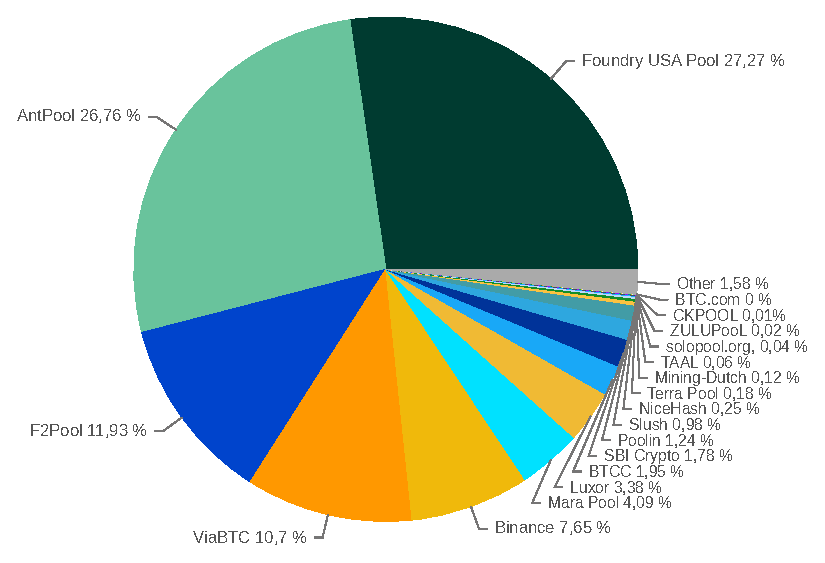
\includegraphics[scale=0.75]{img/hashrate-distribution-coin-dance-week-20231012.eps}
  \caption{Répartition du taux de hachage apparent entre les coopératives de minage de BTC, semaine du 5 au 12 octobre 2023. (source~: \texttt{coin.dance})}
  \label{fig:hashrate-distribution}
\end{figure}

% --- Délégation de la communication pair-à-pair (relais) ---

Un autre défaut inhérent du minage est la latence liée à l'annonce des blocs. Comme expliqué dans la section sur la chaîne la plus longue, cette latence produit des blocs orphelins, qui sont valides mais ne sont pas rattachés à la chaîne principale. Cela fait que des mineurs mal connectés ont une puissance de hachage apparente inférieure à leur puissance de hachage réelle.

Pour tenter d'atténuer les effets de ce défaut, les mineurs ont mis en place des relais de communication permettant de s'envoyer des blocs mutuellement de manière plus efficace en supprimant les protections contre le déni de service nécessaires sur le réseau pair-à-pair ouvert.

Le premier relai a été créé par Matt Corallo sous le nom de \eng{Bitcoin Relay Network}. Il a été lancé en 2013\pagenote{«~Le premier relai [...] a été lancé en 2013~»~: \url{https://lists.linuxfoundation.org/pipermail/bitcoin-dev/2013-November/003596.html}0} et est devenu pleinement fonctionnel en 2015\pagenote{«~[il] est devenu pleinement fonctionnel en 2015~»~: \url{https://web.archive.org/web/20150628233706/https://bitcoinrelaynetwork.org/}.}. Le réseau était composé de plusieurs nœuds spécialisés hébergés sur l'infrastructure Amazon Web Services. Un concurrent était le réseau Falcon, géré par une équipe de l'université Cornell dirigée par Emin Gün Sirer\pagenote{«~Un concurrent était le réseau Falcon~»~: \url{https://web.archive.org/web/20160609081540/https://www.falcon-net.org/}}. Le Bitcoin Relay Network a été remplacé en 2016 par le réseau FIBRE\sendnote{Matt Corallo, \eng{The Future of The Bitcoin Relay Network(s)}, 7 juillet 2016~: \url{https://bluematt.bitcoin.ninja/2016/07/07/relay-networks/}.} (pour \eng{Fast Internet Bitcoin Relay Engine}), un réseau basé sur UDP (protocole alternatif à TCP) qui implémente l'optimisation \texttt{cmpctblock}, toujours géré par Matt Corallo. C'est ce réseau qui est utilisé par la plupart des mineurs aujourd'hui.

% --- Centralisation ---

Cette industrialisation du minage a mené à la centralisation de l'activité minière, à la fois au niveau de la puissance de hachage (fermes de minage) que de la sélection des transactions (coopératives et relais). Si cette agrégation n'est pas fatale (les hacheurs sont libres de quitter leur coopérative pour une autre et les mineurs sont libres de ne pas utiliser le relai), elle n'en diminue pas moins la sécurité minière de la chaîne.

% P2Pool
Certaines améliorations ont été proposées dans le minage pour corriger ce problème. La première est le protocole P2Pool, qui est un protocole de minage coopératif basé sur un réseau pair-à-pair de mineurs\pagenote{«~P2Pool qui est un protocole de minage coopératif basé sur un réseau pair-à-pair de mineurs~»~: \url{http://p2pool.in/}.}. Celui-ci met en communication les hacheurs en se basant sur une chaîne latérale -- la «~chaîne de partage~» -- dont la difficulté est plus faible et qui regroupe les différentes contributions des participants. Le développement de P2Pool sur la version principale de Bitcoin semble avoir été mis en suspens en 2017. Toutefois, le procédé est mis en œuvre sur Monero depuis octobre 2021 au moyen d'une coopérative du même nom\pagenote{«~le procédé est mis en œuvre sur Monero~»~: \url{https://p2pool.io/}.}.

% Stratum V2
Le seconde est le protocole Stratum V2\sendnote{Braiins, \eng{Stratum V2 Protocol Overview}~: \url{https://braiins.com/stratum-v2\#job-selection}.}, \textcolor{darkgray}{actuellement en développement}, qui permettrait (entre autres) aux hacheurs de négocier le contenu des blocs. À défaut de corriger complètement la délégation sur la sélection des transactions, cette nouvelle version de Stratum aurait le mérite de rendre le processus plus transparent.

% Limites
Cependant, ces propositions d'amélioration, bien que louables, ne suppriment pas l'avantage économique découlant de la centralisation, qui se retrouve par ailleurs dans toutes les industries (économie d'échelle). La décentralisation a un coût, et celui-ci ne sera justifié que lorsque le bénéfice apporté le surpassera, c'est-à-dire le jour où le réseau sera réellement attaqué.

\section*{Un algorithme de consensus novateur}
\addcontentsline{toc}{section}{Un algorithme de consensus novateur}

Pour fonctionner en tant que système distribué de monnaie numérique, Bitcoin se base sur un mécanisme de consensus novateur. Celui-ci met en jeu une chaîne de blocs construite par les mineurs, qui sont rémunérés pour leur travail. Chaque bloc est un ensemble horodaté de transactions, qui contient une preuve de travail quantifiant l'énergie dépensée. Le consensus est atteint par la sélection de la plus longue chaîne.

Cet algorithme de consensus a un fonctionnement objectif, ouvert et robuste, ce qui explique le succès de Bitcoin par rapport à ses prédécesseurs. Par son aspect essentiellement économique, il donne au système une très grande résistance à la double dépense opportuniste, notamment grâce à la gigantesque industrie minière qui le soutient.

Il existe cependant une menace plus importante, plus insidieuse~: celle de la censure, dont nous parlerons dans le prochain chapitre.
% Copyright (c) 2023 Ludovic Lars
% This work is licensed under the CC BY-NC-SA 4.0 International License

\chapter{La résistance à la censure}
\label{ch:censure}
\label{enotezch:9}

\lettrine[]{L}'un des problèmes croissants de notre époque est la censure financière. Avec le développement de l'économie mondialisée, reposant notamment sur Internet, le recours aux intermédiaires financiers est devenu de plus en plus courant. Cette évolution fait que l'entrave de transferts monétaires constitue aujourd'hui une complication générale, expérimentée par une part grandissante de la population.

Bitcoin forme une solution à ce problème. L'une de ses caractéristiques primordiales est en effet sa résistance à la censure, c'est-à-dire le fait qu'il est difficile pour une entité quelconque d'empêcher la réalisation d'un paiement. En permettant «~aux paiements en ligne d'être envoyés directement d'une partie à l'autre sans passer par une institution financière~», Bitcoin contourne l'arsenal de contrôles financiers qui gangrènent nos moyens de paiement et d'épargne modernes.

La résistance à la censure est, comme la confirmation des transactions, un mécanisme économique. Elle se fonde de manière essentielle sur la preuve de travail ainsi qu'elle est appliquée dans l'algorithme de consensus de Nakamoto. De ce fait, les alternatives proposées comme les algorithmes de preuve d'enjeu montrent une résistance à la censure bien plus faible.

Dans ce chapitre, nous verrons d'abord comment la censure financière intervient dans le monde bancaire aujourd'hui et pourquoi elle devrait se généraliser à l'avenir avec le déploiement des monnaies numériques de banque centrale. Puis, nous décrirons de quelle façon la censure peut s'exercer dans Bitcoin et comment le système peut y résister. Nous expliquerons enfin en quoi les propositions alternatives ne suffisent pas.

\section*{Qu'entendons-nous par censure financière~?}
\addcontentsline{toc}{section}{Qu'entendons-nous par censure financière~?}

% https://www.universalis.fr/encyclopedie/censure/
%
% Censure (sens étroit) = restriction
% Censure (sens large) = manifestation spécifique de l'autorité qui vient entraver un discours ou une action
% Censure financière = inhibition de l'expression ou de l'action d'une entité par la restriction directe de son activité financière

% Description introductive de la censure
La notion de censure peut paraître étrange de prime abord quand on parle de monnaie. Au sens courant, la censure désigne la restriction de l'expression, notamment par l'interdiction de la diffusion de certaines idées. Néanmoins, il est possible de la comprendre dans un sens plus large, qui mêle paiement et expression.

% Origine du terme, insitution des censeurs à Rome
Le terme de censure vient du latin \emph{censeo} signifiant «~évaluer~», «~estimer~», «~déclarer~», «~juger~». Il trouve son origine dans une institution importante de la République romaine, celle des censeurs, deux magistrats qui avaient pour charge de procéder au dénombrement des citoyens et de leurs biens (le \emph{census}), de collecter les impôts, de superviser les travaux publics, de gérer la liste des personnes admises au Sénat (l'\emph{album senatorium}) et de veiller au maintien des «~bonnes mœurs~» de la population en administrant des blâmes ou des peines temporaires. La première fonction des censeurs a donné sa signification au mot recensement. La seconde aux concepts de cens et de suffrage censitaire. Et la dernière a été à l'origine de ce que nous appelons la censure.

% Censure religieuse
Au Moyen Âge, le mot latin \emph{censura} a été repris par le catholicisme pour prendre un sens religieux et se limiter ainsi au discours, et en particulier aux textes. La censure s'apparentait alors à un blâme (sens encore parfois employé, notamment en matière de critique littéraire) ou à une interdiction. Elle se caractérisait par la relecture et la correction des ouvrages rédigés pour s'assurer que tout était conforme au dogme de l'Église catholique romaine.

% Censure politique
Néanmoins, l'apparition de l'imprimerie au \textsc{xv}\ieme{}~siècle a bouleversé les choses~: le nombre de livres a explosé, et ce faisant, a retiré le contrôle que la hiérarchie catholique avait sur la publication des écrits, contrôle qui a été transféré à l'État. La censure a par conséquent acquis son sens politique actuel, en désignant l'examen que le pouvoir étatique fait préalablement des livres, journaux, pièces de théâtre,~etc., pour en permettre ou en prohiber la publication ou la représentation. Par la suite, le terme a fini par nommer toute atteinte à la liberté d'expression, quel que soit le support, que cela se fasse avant (censure a priori) ou après la diffusion (censure a posteriori).

% Censure privée
Avec le développement des médias de masse (journaux, radio, télévision) et surtout des médias sociaux, le terme a acquis un sens élargi et on s'est mis à parler de censure pour tout choix d'édition pris par une entité privée vis-à-vis de ses clients ou de ses utilisateurs. Cette censure privée n'est pas une atteinte à la liberté d'expression au sens strict, mais elle pose problème lorsque le domaine est monopolisé par un petit nombre d'acteurs bénéficiant souvent d'un avantage légal ou d'une subvention étatique. De plus, cette censure peut être directement l'émanation d'une intervention politique, la plateforme en question ne faisant qu'appliquer les directives générales du pouvoir\footnote{Voir par exemple l'affaire des Twitter Files qui a révélé les manœuvres internes et l'intervention de l'État fédéral des États-Unis dans la politique de censure de la plateforme. -- Evan Perez, Donie O'Sullivan, Brian Fung, «~\eng{No directive: FBI agents, tech executives deny government ordered Twitter to suppress Hunter Biden story}~», \emph{CNN}, 23 décembre 2022~: \url{https://edition.cnn.com/2022/12/23/politics/twitter-files-elon-musk-fbi-hunter-biden-laptop/index.html}.}. % Cet état de fait a été illustré par les Twitter Files, publiés à partir de décembre 2022, suite à la prise de possession de la plateforme de microblogage Twitter par Elon Musk, qui ont révélé les manœuvres internes et l'intervention de l'État fédéral des États-Unis dans la politique de censure de la plateforme. Le FBI a notamment reconnu la véracité de cette situation~: «~La correspondance entre le FBI et Twitter ne montre rien d'autre que des exemples de nos engagements traditionnels, de longue date et toujours en cours, entre le gouvernement fédéral et le secteur privé, qui impliquent de nombreuses entreprises dans de multiples secteurs et industries. Comme le montre la correspondance, le FBI fournit des informations essentielles au secteur privé afin de lui permettre de se protéger et de protéger ses clients. Les hommes et les femmes du FBI travaillent chaque jour pour protéger le public américain. Il est regrettable que des théoriciens du complot et d'autres personnes alimentent la désinformation auprès du public américain dans le seul but de tenter de discréditer l'agence.~» -- "The correspondence between the FBI and Twitter show nothing more than examples of our traditional, longstanding and ongoing federal government and private sector engagements, which involve numerous companies over multiple sectors and industries. As evidenced in the correspondence, the FBI provides critical information to the private sector in an effort to allow them to protect themselves and their customers. The men and women of the FBI work every day to protect the American public. It is unfortunate that conspiracy theorists and others are feeding the American public misinformation with the sole purpose of attempting to discredit the agency."

% Censure financière (sens étroit)
Cependant, cette censure de l'expression peut également être réalisée par l'atteinte de l'activité économique de celui qui s'exprime. En effet, en restreignant la capacité à gagner de l'argent d'une personne et en lui faisant comprendre que son discours pose problème, on peut l'amener à taire ce discours. C'est dans ce contexte qu'a émergé le concept de censure financière, ou \eng{financial censorship} en anglais, que l'organisation internationale \eng{Students for Liberty} définit comme le fait de «~restreindre l'activité financière d'une entité privée, de manière à inhiber ses opérations, avec l'intention implicite de la réduire au silence\footnote{Students for Liberty, \eng{Financial Censorship}~: \url{https://studentsforliberty.org/blog/freedom-of-expression/financial-censorship/}.}~». C'est aussi le sens que lui donne l'\eng{Electronic Frontier Foundation}\pagenote{«~C'est aussi le sens que lui donne l'\eng{Electronic Frontier Foundation}~»~: Electronic Frontier Foundation, \eng{Financial Censorship}~: \url{https://www.eff.org/issues/financial-censorship}.}. % Financial censorship involves the restriction of a private entity's financial activity, in such a way as to inhibit their operations, with the implicit intention of rendering them silent.

% Censure financière (sens large)
Mais les répercussions du contrôle financier ne s'arrêtent pas à l'expression et peuvent concerner l'action humaine en général. Ainsi, la censure financière peut être saisie dans un sens plus large, une signification par exemple adoptée par trois chercheurs de l'université d'État de San José qui affirment que «~la censure financière se produit lorsqu'une institution financière refuse ses services à une partie en raison des opinions exprimées, des actions ou du secteur d'activité de cette partie\footnote{Marco Pagani, George Whaley, David Czerwinski, «~\eng{Frameworks for Assessing Financial Censorship and Its Implications}~», in \eng{Journal of Accounting and Finance}, vol.~22, no.~1, 2022~: \url{https://articlegateway.com/index.php/JAF/article/download/4989/4759}.}~». % Financial censorship occurs when a financial institution denies its services to a party because of that party's expressed views, actions, or line of business.

% Censure comme restriction financière arbitraire
Enfin, on peut comprendre la censure financière comme la restriction financière elle-même à condition qu'elle repose sur un critère subjectif externe (respect de normes arbitraires) et non pas sur une donnée économique objective, comme par exemple le paiement d'une commission. La censure peut être appliquée de manière publique (interdiction légale d'une transaction), privée (par une banque par exemple) ou les deux. Cette définition conserve toujours en elle l'idée de modeler le comportement extérieur de la personne par l'intervention sur ses finances. C'est notamment cette signification qui est donnée à la censure dans Bitcoin.

% Définition générale
Au sens général, la censure financière consiste donc à restreindre directement l'activité financière d'une entité de façon à inhiber son expression ou son action. L'idée est d'influencer l'individu par le contrôle sur la monnaie dont il se sert, un outil qui est essentiel à sa survie économique. Aujourd'hui, la censure s'applique essentiellement au crédit bancaire, dont les transferts sont hautement réglementés par le pouvoir. Demain, elle pourra concerner la monnaie numérique gérée par la banque centrale.

\section*{La banque et la censure}
\addcontentsline{toc}{section}{La banque et la censure}

% Censure financière avec l'argent liquide
La censure financière s'exerce par la maîtrise sur le transfert de monnaie, de sorte que cette censure peut difficilement s'appliquer à l'argent liquide physique. En effet, ce dernier (qu'il prenne la forme de pièces de métal précieux ou de billets fiduciaires) permet l'échange direct et confidentiel de personne à personne, ce qui empêche la mise en place de toute restriction en dehors de quelques cas particuliers.

% Censure financière avec un compte bancaire
En revanche, dans le domaine bancaire, le client dispose d'un compte courant sur lequel la banque inscrit les crédits et gère les transferts. La restriction financière est de ce fait beaucoup plus simple~: la banque peut sélectionner les transferts, geler le compte momentanément et même refuser le retrait d'argent. C'est aussi le cas de tous les services construits au-dessus du système bancaire traditionnel, comme PayPal.

% Accroissement
C'est donc tout naturellement que l'accroissement de la censure financière a coïncidé avec la bancarisation de la société, qui a eu lieu à partir des années 1960 en Occident\pagenote{«~la bancarisation de la société, qui a eu lieu à partir des années 1960 en Occident~»~: \url{https://books.openedition.org/pur/121053?lang=fr}~; \url{https://www.the-american-interest.com/2019/02/25/bigger-fewer-riskier-the-evolution-of-u-s-banking-since-1950/}.}, et qui s'est caractérisée par la généralisation de l'usage du compte courant et des moyens de paiement apparentés comme le chèque bancaire, la carte de crédit et le virement. En quelques décennies, le paiement a migré vers le domaine bancaire, favorisé par la loi et bien plus commode à utiliser que les espèces, dont l'utilisation a elle-même été restreinte légalement. D'où la meilleure efficacité de la censure~: si le liquide ne permet plus de gérer ses affaires convenablement, alors la possibilité de se retirer complètement du système bancaire n'est plus une option viable.

% Surveillance financière
Cette censure a été mise en place par l'intermédiaire de la surveillance financière, qui est aujourd'hui particulièrement fréquente dans l'industrie bancaire. Les banques ont en effet l'obligation légale de surveiller leurs clients et d'intervenir dans le cas où elles constatent un comportement «~suspect~» de leur part, en empêchant leurs virements ou en gelant leurs comptes. Elles ne font pas cela de gaieté de cœur~: elles ne procèdent pas à la surveillance de leurs clients pour les «~protéger~», mais pour se protéger elles-mêmes contre les éventuelles complications liées à la réglementation.

% Lutte contre le blanchiment d'argent : guerre contre la drogue
Cette réglementation s'est développée à mesure que l'activité bancaire se popularisait. À partir des années 70, le prétexte de la lutte contre le blanchiment d'argent (notamment dans le cadre de la guerre contre la drogue) s'est imposé comme le principal prétexte derrière les restrictions imposées aux banques. Aux États-Unis notamment, la réglementation bancaire s'est particulièrement durcie suite à l'adoption du \eng{Bank Secrecy Act} de 1970, qui se proposait de lutter contre le blanchiment d'argent.

% Lutte contre le blanchiment d'argent : web
Puis, avec l'apparition du web dans les années 1990, l'utilisation des banques internationales a demandé une réglementation accrue. Différents organismes de surveillance ont ainsi été créés. Le Groupe d'action financière (GAFI), un organisme intergouvernemental émettant régulièrement des recommandations de normes réglementaires et de sanctions économiques, a été créé en juillet 1989 dans le but de lutter contre le blanchiment d'argent. Le Financial Crimes Enforcement Network (FinCEN), le bureau du département du Trésor des États-Unis qui collecte et analyse les informations sur les transactions financières, a été formé dans ce sens le 25 avril 1990. L'équivalent français, la cellule TRACFIN (Traitement du renseignement et action contre les circuits financiers clandestins), est apparu en juillet 1990. Du côté européen, la première directive de l'Union Européenne relative à la prévention de l'utilisation du système financier aux fins du blanchiment de capitaux est datée du 10 juin 1990\pagenote{«~la première directive de l'Union Européenne relative à la prévention de l'utilisation du système financier aux fins du blanchiment de capitaux~»~: \url{https://eur-lex.europa.eu/legal-content/FR/TXT/PDF/?uri=CELEX:31991L0308&from=FR}.}.

% Lutte contre le financement du terrorisme
Enfin, après les attentats islamistes du 11 septembre 2001, un autre prétexte est apparu~: la lutte contre le financement du terrorisme. Celle-ci s'est matérialisée aux États-Unis par l'adoption du \eng{PATRIOT Act} en octobre 2001, dont le Titre 3 concerne les restrictions financières. En France, la loi du 15 novembre 2001 relative à la sécurité quotidienne a requalifié «~le fait de financer une entreprise terroriste~» comme un acte de terrorisme en lui-même\footnote{Code pénal, Article 421-2-2, 15 novembre 2001.}. La surveillance financière s'est renforcée en conséquence. % \url{https://www.legifrance.gouv.fr/codes/article_lc/LEGIARTI000006418433}

% LCB-FT et connaissance du client
Ces deux évolutions forment la base de ce qu'on appelle généralement la lutte contre le blanchiment des capitaux et le financement du terrorisme (LCB-FT) en France et les normes AML/CFT (pour \eng{Anti-Money Laundering/Combating the Financing of Terrorism}) aux États-Unis. Ce resserrement se caractérise notamment par la connaissance du client (\eng{Know Your Customer} ou KYC), une pratique également appelée vigilance à l'égard de la clientèle, qui consiste à vérifier l'identité, la conformité et les risques liés à chaque client. Cette exigence d'identification s'est insérée dans tous les services financiers aujourd'hui.

% Fin du secret bancaire
En conséquence, le secret bancaire, c'est-à-dire l'obligation pour les banques de ne pas livrer des informations sur leurs clients à des tiers, a fini par disparaître\pagenote{«~le secret bancaire [...] a fini par disparaître~»~: Anthony Amicelle, Jean Bérard, \eng{Vers la fin du secret bancaire ou de la vie privée~?}, 2019~: \url{https://journals.openedition.org/conflits/21291}.}, y compris en Suisse\pagenote{«~y compris en Suisse~»~: Mathilde Damgé, \eng{Comment la Suisse a renoncé au secret bancaire}, 11 février 2015~: \url{https://www.lemonde.fr/evasion-fiscale/article/2015/02/11/comment-la-suisse-a-renonce-au-secret-bancaire_4572485_4862750.html}.}. L'usage d'un compte bancaire aujourd'hui présuppose la surveillance générale des transactions et l'inspection minutieuse des opérations les moins usuelles. Ainsi, il est aujourd'hui impossible de virer une importante somme d'argent d'un compte à un autre sans devoir fournir une justification.

% Résumé par Jonathan Thornburg
Cette situation du domaine financier a été résumée en janvier 2009 par Jonathan Thornburg sur la liste de diffusion en réponse à Satoshi Nakamoto qui décrivait les utilisations qu'on pouvait faire de Bitcoin~:

\begin{quote}
«~Dans le monde moderne, aucun État important ne veut autoriser des transactions financières internationales intraçables au-delà d'un certain seuil relativement modeste. (Les mots d'ordre habituels incluent des expressions telles que “blanchiment de l'argent de la drogue”, “évasion fiscale”, et\,/\,ou “financement du terrorisme”). À cette fin, les transactions financières électroniques sont actuellement surveillées par divers États et leurs agences, et toutes les transactions, sauf les plus petites, sont désormais soumises à diverses exigences en matière d'identification pour les personnes se trouvant à chaque extrémité\footnote{Jonathan Thornburg, \eng{Re: Bitcoin v0.1 released}, \wtime{17/01/2009 16:49:45 UTC}~: \url{https://www.metzdowd.com/pipermail/cryptography/2009-January/015016.html}.}.~»
\end{quote} % "In the modern world, no major government wants to allow untracable international financial transactions above some fairly modest size thresholds.  (The usual catch-phrases are things like "laundering drug money", "tax evasion", and/or "financing terrorist groups".) To this end, electronic financial transactions are currently monitored by various governments & their agencies, and any but the smallest of transactions now come with various ID requirements for the humans on each end."

\section*{Les cas de censure financière}
\addcontentsline{toc}{section}{Les cas de censure financière}

% Comme on l'a dit, la censure financière peut concerner l'expression, l'action ou l'activité professionnelle d'une personne. Il s'agit donc d'appliquer la censure dans le but d'entraver une action dérangeante, comme un discours dissonant, une opposition politique non tolérée, un comportement inapproprié, une profession jugée immorale,~etc. Si vous dépendez d'un compte bancaire, vous devez vous taire sur certains sujets, ne pas vous engager dans certaines actions politiques et ne pas exercer certaines professions, auquel cas vous pourriez être punis indirectement.

Au cours des dernières années, les cas célèbres de censure financière se sont multipliés, à tel point qu'il est impossible d'en faire une liste exhaustive. Nous nous contenterons d'en citer les exemples les plus manifestes en Occident, tout en gardant en tête que cette censure n'est généralement pas rendue publique par ceux qui la subissent.

% Nous nous bornerons ici à évoquer le système financier occidental, et notamment celui des États-Unis. Le pays américain est censé être le pays le plus libre au monde et donne une bonne idée de la progression de cette censure.

% WikiLeaks
L'exemple le plus connu est probablement le blocus financier contre WikiLeaks mis en place par Mastercard, Visa, Western Union, Bank of America et d'autres acteurs, en décembre 2010, dans le but de faire taire l'organisation. En octobre 2011, un communiqué de WikiLeaks a indiqué que le blocus financier avait fait disparaître 95~\% de ses revenus\pagenote{«~le blocus financier avait fait disparaître 95~\% de ses revenus~»~: WikiLeaks, \eng{Banking Blockade}, \wtime{24/10/2011 13:00 UTC}, \url{https://wikileaks.org/Banking-Blockade.html}.}. Cette affaire a eu des répercussions directes dans l'histoire de Bitcoin, comme nous l'avons raconté dans le chapitre~\ref{ch:mythe}.

% Opération Choke Point
Un autre cas, qui visait cette fois la profession des personnes censurées, est l'opération Choke Point mise en place entre 2013 et 2017 par le département de la Justice des États-Unis\pagenote{«~opération Choke Point mise en place entre 2013 et 2017 par le département de la Justice des États-Unis~»~: \url{https://en.wikipedia.org/wiki/Operation_Choke_Point}~; \url{https://www.wsj.com/articles/SB10001424127887323838204578654411043000772}, archive~: \url{https://archive.is/bF8KZ}.}. L'opération avait pour but d'«~étouffer~» certains secteurs d'activité en restreignant leur accès au crédit et à d'autres services bancaires. Ces activités jugées «~à haut risque~» incluaient le prêt sur gages ou sur salaire, le jeu d'argent, la pornographie, l'escorting, mais aussi la vente de tabac et de produits pharmaceutiques, la vente de pièces de monnaie, les services de rencontre ou encore l'organisation des clubs de voyage. La vente d'armes et de munitions était aussi concernée~: Defense Distributed, l'entreprise du crypto-anarchiste libertarien Cody Wilson, spécialisée dans la diffusion de schémas de conception d'armes à feu fabriquées par imprimante 3D, en a fait les frais en 2015 en subissant une fermeture de ses comptes par Chase, PayPal et Stripe\pagenote{«~en subissant une fermeture de ses comptes par Chase, PayPal et Strip~»~: Kelsey Bolar, \eng{Firearms Sellers Say They're Being Choked Off From Payment Processors}, 12 janvier 2015~: \url{https://www.dailysignal.com/2015/01/12/firearms-sellers-say-theyre-choked-off-payment-processors/}.}.

% La censure financière concerne également l'opinion politique, qu'elle contribue par là à modeler. Ainsi, les activistes politiques dont les positions sont jugées extrêmes par les élites ont régulièrement des problèmes avec les différents services financiers qu'ils utilisent.

% Alt-right étasunienne (InfoWars), extrême-droite française (Égalité et Réconciliation)
En 2018, c'est l'opinion politique qui a dû endurer la censure. De nombreuses personnalités et organisations d'\eng{alt-right} américaine ont ainsi été bannies des divers réseaux sociaux et ont perdu l'accès à divers services financiers. L'exemple le plus emblématique était Alex Jones, fondateur du site de réinformation InfoWars, qui, outre sa purge des médias sociaux durant l'été 2018, a vu son compte PayPal être clôturé\pagenote{«~Alex Jones [...] a vu son compte PayPal être clôturé~»~: Brian Fung, \eng{PayPal bans Alex Jones, saying Infowars 'promoted hate or discriminatory intolerance'}, 21 septembre 2018~: \url{https://www.washingtonpost.com/technology/2018/09/21/paypal-bans-alex-jones-saying-infowars-promoted-hate-or-discriminatory-intolerance/}}. On peut aussi citer les cas du média social Gab (chassé de PayPal, Stripe Cash App et Coinbase\pagenote{«~chassé de PayPal, Stripe Cash App et Coinbase~»~: \url{https://www.bitcoininsider.org/article/44690/after-coinbase-paypal-bans-social-media-platform-gab-just-because}.}), de Milo Yiannopoulos (banni de PayPal pour avoir fait un salut nazi\pagenote{«~banni de PayPal pour avoir fait un salut nazi~»~: \url{https://www.timesofisrael.com/paypal-suspends-milo-yiannopoulos-over-nazi-based-trolling-of-jewish-journalist/}.}) ou encore de Robert Spencer (chroniqueur du blog anti-islam Jihad Watch, chassé de Patreon suite à la pression de Mastercard\pagenote{«~chassé de Patreon suite à la pression de Mastercard~»~: \url{https://twitter.com/Patreon/status/1029551216886341634}.}). En France, cette censure s'est manifestée à l'encontre d'Égalité et Réconciliation, l'association de l'antisioniste Alain Soral, qui a été exclue de PayPal en août 2018, dans le cadre d'une purge similaire à celle des militants américains. L'association a également vu plusieurs de ses comptes bancaires (Banque postale, BNP Paribas, Banque populaire) être fermés au cours des années\pagenote{«~L'association a également vu plusieurs de ses comptes bancaires (Banque postale, BNP Paribas, Banque populaire) être fermés~»~: Égalité et Réconciliation, \eng{Soutenez-nous~: la Banque populaire ferme le compte en banque d'Égalité \& Réconciliation}, 6 février 2022~: \url{https://www.egaliteetreconciliation.fr/Soutenez-nous-la-Banque-populaire-ferme-le-compte-en-banque-d-Egalite-Reconciliation-67155.html}.}.

% Des comptes d'organisations liées au mouvement Antifa (Atlanta Antifa, Antifa Sacramento, Anti-Fascist Network) ont également été suspendus de PayPal en novembre 2018\footnote{\url{https://www.newsweek.com/paypal-cancels-alt-right-antifa-accounts-1209838}}.

% Manifestations de Hong Kong (2019-2020)
Toujours dans le domaine politique, mais en Chine cette fois-ci, on peut citer le cas du mouvement contre l'amendement de la loi d'extradition par le gouvernement de Hong Kong, série de manifestations ayant eu lieu entre mars 2019 et juillet 2020, qui a dû subir les interventions du conglomérat bancaire international HSBC, probablement sous pression de l'État central chinois. En novembre 2019, la filiale de Hong Kong a en effet décidé de fermer un compte utilisé pour soutenir le mouvement de protestation. Puis, elle a gelé le compte du démocrate Ted Hui en décembre 2020\pagenote{«~elle a gelé le compte du démocrate Ted Hui en décembre 2020~»~: \url{https://hongkongfp.com/2020/12/07/hsbc-re-freezes-accounts-belonging-to-family-of-exiled-democrat-ted-hui-amid-hong-kong-police-money-laundering-probe/}.}. Par ailleurs, on a appris en 2023 qu'elle refusait aux Hongkongais ayant fui au Royaume-Uni d'accéder légitimement à leurs fonds de pension, pour un montant s'élevant à 2,2 milliards de livres sterling\pagenote{«~elle refusait aux Hongkongais ayant fui au Royaume-Uni d'accéder légitimement à leurs fonds de pension, pour un montant s'élevant à 2,2 milliards de livres sterling~»~: \url{https://www.lefigaro.fr/flash-eco/hsbc-complice-de-violation-des-droits-humains-a-hong-kong-selon-un-rapport-parlementaire-20230208}, \url{https://www.telegraph.co.uk/business/2023/08/07/hsbc-exececutive-apologises-calling-uk-weak-on-china/}.}.

% Covid-19, Viruswaarheid
Plus récemment, la pandémie de Covid-19 a fourni d'autres occurrences de censure financière. De nombreux activistes opposés aux mesures coercitives comme le confinement, le port du masque et la vaccination obligatoire, ont ainsi été largement censurés, généralement accusés de propager la désinformation. Le groupe d'action néerlandais Viruswaarheid -- s'opposant à la distanciation sociale, au confinement, au couvre-feu et au programme de vaccination -- a ainsi vu son compte bancaire utilisé pour recevoir des donations être fermé par ING Bank en février 2021\pagenote{«~Viruswaarheid [...] a ainsi vu son compte bancaire utilisé pour recevoir des donations être fermé par ING Bank en février 2021~»~: Andreas Kouwenhoven et Wilmer Heck, \eng{De complotdenker bankiert maar elders, zegt de bank}, 17 août 2021~: \url{https://www.nrc.nl/nieuws/2021/08/17/de-complotdenker-bankiert-maar-elders-zegt-de-bank-a4055125}~; archive~: \url{https://archive.is/8LI0k}.}.

% Convoi de la liberté, 2022
Mais l'exemple qui ressort du lot est le mouvement canadien du «~Convoi de la liberté~» de février 2022, initié par les camionneurs qui s'opposaient à l'obligation vaccinale imposée pour entrer sur le territoire par voie terrestre et qui ont manifesté leur mécontentement en faisant route jusqu'à Ottawa pour occuper la ville. Ce mouvement a fait face à une censure financière drastique. Il a dans un premier temps été victime des plateformes de financement participatif, qui ont annulé ses différentes campagnes qui avaient pour objectif de payer le déplacement des camionneurs~: celle de GoFundMe, ayant réuni 10 millions de dollars canadiens, a été retirée le 4 février\pagenote{«~celle de GoFundMe, ayant réuni 10 millions de dollars canadiens, a été retirée le 4 février~»~: Radio-Canada, \eng{La campagne de sociofinancement du convoi des camionneurs retirée de GoFundMe}, 4 février 2022~: \url{https://ici.radio-canada.ca/nouvelle/1859918/retrait-campagne-gofundme-convoi-camionneurs-2022}.}~; tandis que les fonds récupérés par les campagnes organisées sur la plateforme chrétienne GiveSendGo (9 millions de dollars environ) ont été gelés par le gouvernement ontarien, et n'ont pas pu être distribués\pagenote{«~les fonds récupérés par les campagnes organisées sur la plateforme chrétienne GiveSendGo [...] ont été gelés par le gouvernement ontarien~»~: Stephanie Taylor, \eng{Ontario court freezes access to donations for truckers' protest from GiveSendGo}, 10 février 2022~: \url{https://www.ctvnews.ca/canada/ontario-court-freezes-access-to-donations-for-truckers-protest-from-givesendgo-1.5776674}.}. La répression financière s'est considérablement amplifiée lorsque, suite à l'entrée en vigueur de l'état d'urgence déclaré par Justin Trudeau le 14 février, le gouvernement canadien a décidé de geler des comptes bancaires personnels ou professionnels en lien avec le mouvement~: 280 comptes contenant 8 millions de dollars au total ont été gelés de la sorte\pagenote{«~280 comptes contenant 8 millions de dollars au total ont été gelés de le sorte~»~: Bill Curry, Marsha McLeod, \eng{Deputy Minister of Finance describes race against time to prevent economic damage from border blockades}, 17 novembre 2022~: \url{https://www.theglobeandmail.com/politics/article-emergencies-act-inquiry-michael-sabia/}.}. L'année suivante, le juge Paul Rouleau, chargé de la Commission sur l'état d'urgence, a déclaré que le gel des comptes bancaires était un «~outil puissant pour décourager la participation [aux manifestations] et inciter les manifestants à abandonner\footnote{Rob Gillies, «~\eng{Judge: Canada right to invoke emergency act in truck protest}~», \eng{Associated Press News}, 17 février 2023~: \url{https://apnews.com/article/canada-government-justin-trudeau-ottawa-montana-9c1e37aa86d4315703e69f7794637e7f}.}~». % \footnote{The Post Millennial sur Twitter, \wtime{17/02/2023 20:53 UTC}~: \url{https://twitter.com/TPostMillennial/status/1626686280108068872}.}

% Mais l'exemple qui ressort du lot est l'évènement qui a eu lieu au Canada en février 2022 dans le cadre du mouvement de protestation canadien contre l'obligation vaccinale imposée aux personnes entrant sur le territoire par voie terrestre, couramment appelé le Convoi de la liberté. En réaction à cette restriction introduite le 15 janvier 2022 par le gouvernement, des camionneurs (principaux concernés) ont fait route jusqu'à Ottawa pour s'y rejoindre le 29 janvier et exprimer leur mécontentement à l'égard du pouvoir, notamment par des coups de klaxons répétitifs. Le mouvement était globalement non violent et familial. Plus tard, des blocages ont été organisés, dont notamment celui du pont Ambassadeur, faisant la jonction avec les États-Unis entre Détroit et Windsor et cœur névralgique des échanges commerciaux entre les deux pays, sur lequel la circulation a été interrompue entre le 8 et le 13 février. Ces blocages ont servi de prétexte pour l'intervention du gouvernement fédéral canadien de Justin Trudeau, qui a déclaré l'état d'urgence le 14 février en invoquant la Loi sur les mesures d'urgence.
%
% Ce mouvement a dû faire face à une censure financière drastique. D'abord, il a été victime des plateformes de financement participatif, qui ont annulé ses différentes campagnes qui avaient pour objectif de payer le déplacement des camionneurs. La première campagne réalisée sur GoFundMe, ayant recueilli plus de 10 millions de dollars canadiens a ainsi été retirée de la plateforme le 4 février pour cause de «~promotion de la violence et du harcèlement~» suite à la suggestion du maire d'Ottawa. De même, les fonds recueillis par les campagnes organisées sur la plateforme chrétienne GiveSendGo -- totalisant environ 9 millions de dollars canadiens -- ont pu être gelés par le gouvernement de l'Ontario à partir du 10 février, interdisant par là leur distribution.

% Durcissement des sanctions économiques à l'égard de la Russie
Un autre évènement important survenu durant le mois de février est le durcissement des sanctions économiques mises en place par les États occidentaux contre la Russie, suite à son invasion de l'Ukraine\pagenote{Les sanctions économiques internationales qui concernent le domaine financier rentrent dans la catégorie de la censure financière. Celles-ci ont en effet pour but premier d'empêcher le commerce avec la population gouvernée par un État ennemi. Le cas des Russes n'est pas un cas isolé, et de nombreuses autres populations n'ont pas accès aux services financiers disponibles pour les Occidentaux, comme les Palestiniens par exemple. Voir à ce sujet Electronic Frontier Foundation, \eng{Why Is PayPal Denying Service to Palestinians?}, 12 octobre 2021~: \url{https://www.eff.org/deeplinks/2021/10/why-paypal-denying-service-palestinians}.}. Les sanctions financières incluaient l'exclusion de certaines banques russes du système SWIFT, la prohibition du financement en Russie et de l'achat de roubles, et l'interdiction de la fourniture de services de portefeuille, de compte ou de conservation de crypto-actifs. De manière générale, les virements vers la Russie ont été interdits, de sorte que les citoyens russes exilés ne pouvaient plus envoyer d'argent à leur famille. C'est aussi le cas des ressortissants ukrainiens dont les proches sont restés sur le territoire occupé par l'armée russe, comme cette Ukrainienne réfugiée en France qui ne pouvait pas envoyer un virement bancaire de 100~euros à ses parents à Donetsk\pagenote{Ben Canton, \emph{Un an de guerre en Ukraine~: la petite histoire de Valériia et de Binance}, 24 février 2023~: \url{https://journalducoin.com/analyses/un-an-guerre-ukraine-petite-histoire-valeriia-binance/}.}. % Source : https://eur-lex.europa.eu/legal-content/EN/TXT/?uri=CELEX%3A02014R0833-20221217

% RT France
Du côté occidental, des mesures financières ont également été prises dans le but de faire respecter la censure des médias financés par le Kremlin. En janvier 2023, la chaîne d'information RT France, qui était déjà interdite de diffusion en Europe, mais qui continuait d'être accessible sur Internet, a ainsi subi le gel de ses avoirs, ce qui l'a contrainte à fermer définitivement\pagenote{«~RT France [...] a ainsi subi le gel de ses avoirs~»~: Le Parisien, \emph{RT France, branche française de la chaîne russe, annonce sa fermeture}, 23 janvier 2022~: \url{https://www.leparisien.fr/international/rt-france-branche-francaise-de-la-chaine-russe-annonce-sa-fermeture-21-01-2023-YMOTSTASWZAF3KSGCYHAFFMG6U.php}.}.

% Activités liées aux cryptomonnaies

Enfin, pour finir à propos des différentes occurrences de censure financière, on ne peut pas ne pas évoquer les activités liées aux cryptomonnaies, qui ont subi et continuent de subir des restrictions de la part des organismes financiers. L'achat de cryptomonnaies est entravé par les banques qui interdisent régulièrement à leurs clients (toujours en prétendant les «~protéger~») d'envoyer des fonds vers les plateformes de change\pagenote{«~L'achat de cryptomonnaies est entravé par les banques qui interdisent régulièrement à leurs clients [...] d'envoyer des fonds vers les plateformes de change~»~: Jean-Luc (Bitcoin.fr), \emph{Les banques et Bitcoin –- Classement de janvier 2023}, 9 janvier 2023~: \url{https://bitcoin.fr/bitcoin-et-les-banques-classement-de-janvier-2023/}.}. De plus, les entreprises du secteur peinent régulièrement à ouvrir un compte bancaire en raison de la méfiance des acteurs traditionnels\sendnote{Dans son livre \emph{Cryptomonnaie~: la nouvelle guerre}, François-Xavier Thoorens explique par exemple comment lui et sa famille ont été expulsés de leur banque familiale après avoir voulu ouvrir un compte professionnel pour recevoir des fonds récupérés lors de l'ICO d'Ark (pp.~91 -- 97). Mais son cas est loin d'être une exception.}.

% Pouvoir ésotérique
La censure financière est donc de plus en plus fréquente dans notre société. Elle touche de nombreuses personnes de bords politiques opposés, de nationalités diverses et de professions variées. Elle s'exerce bien souvent sans décision juridique spécifique, ce qui donne un caractère ésotérique, caché, arbitraire à l'application du pouvoir réel. C'est ce qui en fait un problème subtil et difficile à expliciter.

% La censure mène à Bitcoin
L'intervention plus prononcée de cette censure a pour effet de pousser les gens à s'intéresser à Bitcoin. En effet, l'expérience d'une telle restriction provoque nécessairement le désir de trouver un moyen de la contourner, quand bien même celle-ci serait légère. Lorsqu'une personne prend pleinement conscience de la censure comme une réalité concrète et non plus comme un risque abstrait, elle ressent le besoin de s'en libérer et de se prémunir de ce danger, ce qui lui démontre (ou lui confirme) la proposition de valeur de Bitcoin\footnote{Cet effet de l'expérience de la censure a été décrit par Nick Szabo au micro de Peter McCormack en 2019~: «~Certaines personnes doivent être frappées par la réalité. Si vous êtes censuré par une banque, comme c'est de plus en plus le cas -- et c'est d'ailleurs l'un des risques de la centralisation numérique -- c'est que les gens soient censurés et les activistes politiques de différents bords commencent à découvrir qu'on peut aller voir les banques et faire taire ses ennemis politiques et les gens qui font des choses qu'on ne veut pas qu'ils fassent, on les fait taire. On n'a pas nécessairement besoin de faire passer une loi, on peut convaincre certains régulateurs ou certains politiciens, et puis ils mettent la pression sur les banques, et boum~: c'est notre loi de facto juste là. Ça se produit de plus en plus souvent parce que la centralisation numérique rend les choses si vulnérables à ça. Il s'agit donc d'une tendance opposée et tout dépend de la vitesse à laquelle elle se développe, car à chaque fois que quelqu'un est censuré, boum~: c'est une réalité qui s'impose à lui et il devient fan de Bitcoin.~» -- What Bitcoin Did Podcast, \eng{Nick Szabo on Cypherpunks, Money and Bitcoin} (audio), 1\ier{} novembre 2019~: \url{https://www.whatbitcoindid.com/podcast/nick-szabo-on-cypherpunks-money-and-bitcoin}.}. C'est le cas de l'auteur de cet ouvrage qui a vu son compte bancaire être gelé sans préavis, sans que la banque ne mentionne la raison derrière cette suspension, et qui n'a pu récupérer ses fonds que six mois plus tard\pagenote{«~C'est le cas de l'auteur de cet ouvrage~»~: Ludovic Lars sur Twitter, \wtime{15/02/2022 10:42 UTC}~: \url{https://twitter.com/lugaxker/status/1493536121678147586}.}.

% "Well some people have to be hitting over the head with reality. If you're censored via bank, as people increasingly are, and by the way, that's one of the risks of digital centralization, is people get censored and the political activists from various points of view are starting to discover that you can go to banks and get your political enemies shut down and people doing things you don't want them to do, you get them shut down. You don't necessarily need to pass a law, you can convince some regulators or convince some politicians and then they lean on the banks and boom, that's your de facto law right there. That's increasingly happening because digital centralization makes things so vulnerable to that. So that's another trend and it depends how fast that grows because every time somebody gets censored, boom, that's a reality over their head, they become a Bitcoin fan.".

\section*{Censure et monnaie numérique de banque centrale}
\addcontentsline{toc}{section}{Censure et monnaie numérique de banque centrale}

% Monnaies numériques de banque centrale

% Si la censure financière constitue aujourd'hui une complication occasionnelle.
La tendance est donc claire~: avec l'utilisation intensive des comptes bancaires en lieu et place des espèces, le pouvoir de censure financière est devenu de plus en plus important. Ainsi, même si cette censure reste aujourd'hui occasionnelle, nous pouvons nous attendre à ce qu'elle constitue un problème grandissant à l'avenir. Plus précisément, elle pourrait devenir une contrainte générale dans les décennies à venir avec le déploiement progressif des monnaies numériques de banque centrale (MNBC) et la disparition conjointe de l'argent liquide.

Tel que nous l'avons vu dans la section dédiée à la monnaie numérique de banque centrale dans le chapitre~\ref{ch:adversaire}, la numérisation de la monnaie constitue la prochaine étape dans l'évolution de la monnaie étatique. Depuis 2016, les banques centrales autour du monde s'efforcent de concevoir des systèmes qui pourraient être utilisés par le grand public et les communications à ce sujet se multiplient depuis 2020.

% Monnaie numérique : seigneuriage + contrôle financier
Une telle monnaie numérique permettrait de récupérer un revenu de seigneuriage supplémentaire en supprimant le coût de la production de l'argent liquide remplacé et en reprenant une part de l'activité monétaire qui a lieu aujourd'hui par l'intermédiaire du crédit émis par les banques commerciales. Mais elle permettrait aussi (ce qui nous intéresse ici) d'exercer un contrôle financier total sur les transactions des citoyens en centralisant la gestion du système entre les mains de la banque centrale et des organismes agréés.

% Surveillance financière
Ce contrôle s'accompagnerait bien entendu d'une surveillance financière accrue, qui serait justifiée par les mêmes prétextes utilisés aujourd'hui, comme la lutte contre le blanchiment d'argent et le financement du terrorisme. Ceci pourrait conduire à l'instauration d'un système panoptique, où la surveillance se ferait à l'insu du surveillé\pagenote{«~un système panoptique, où la surveillance se ferait à l'insu du surveillé~»~: Le panoptique (en anglais, \eng{panopticon}) était un type d'architecture carcérale imaginée par le philosophe utilitariste Jeremy Bentham et son frère Samuel à la fin du \textsc{xviii}\ieme{}~siècle. L'objectif de la structure panoptique était de permettre à un gardien, logé dans une tour centrale, d'observer tous les prisonniers, enfermés dans des cellules individuelles autour de la tour, sans que ceux-ci puissent savoir s'ils étaient observés.}. Les banques centrales nient vouloir aller dans cette direction, mais le fait est qu'elles ne rendront jamais leurs systèmes strictement confidentiels, réservant toujours un droit de regard aux autorités compétentes. % BD "Nous travaillons à protéger la vie privée mais puisque l'argent numérique laisse une trace sur la blockchain, cela ne sera pas entièrement anonyme comme c'est le cas avec un billet de banque", a déclaré lundi 25 septembre 2023 la présidente de la Banque centrale européenne (BCE) devant les députés de la commission des affaires économiques et monétaires du Parlement européen. https://www.bfmtv.com/crypto/christine-lagarde-admet-que-l-euro-numerique-ne-sera-pas-totalement-anonyme_AV-202309260419.html

% Disparition progressive de l'argent liquide
Cette surveillance financière pourrait être affermie par la disparition progressive de l'argent liquide, qui a déjà commencé à certains endroits du monde. C'est le cas de la Suède, où la question de la fin des espèces est déjà discutée et où l'État fait tout pour mettre à disposition des moyens de paiement numérique innovants\pagenote{«~C'est le cas de la Suède [...] où l'État fait tout pour mettre à disposition des moyens de paiement numérique innovants~»~: sweden.se, \eng{A cashless society}~: \url{https://sweden.se/life/society/a-cashless-society}.}. C'est aussi le cas de la Chine, où l'essentiel des transferts se fait par l'intermédiaire de systèmes de paiement mobile comme WeChat Pay et Alipay. Ce n'est pas un hasard si ces deux pays ont été les premiers à envisager sérieusement de développer une monnaie numérique. % et où la banque centrale a également lancé son programme pilote de monnaie numérique

% Démonétisation des espèces
La guerre contre l'argent liquide sévit déjà dans certains pays par le biais de la démonétisation de certains billets en circulation, qui peuvent être échangés contre d'autres billets ou être déposés sur un compte bancaire, à condition d'attester de la provenance des fonds. En Inde en novembre 2016, le gouvernement de Narendra Modi a ainsi démonétisé les billets de 500 et 1~000 roupies, équivalant à 7,5 et 15~\$, et représentant à eux seuls 86~\% de la monnaie en circulation, dans le but affiché de lutter contre la contrefaçon de faux billets, l'évasion fiscale et l'économie informelle\pagenote{«~Narendra Modi a ainsi démonétisé les billets de 500 et 1~000 roupies~»~: Ninon Renaud, Michel De Grandi, \emph{En Inde, la démonétisation des grosses coupures provoque l'émoi}, 13 novembre 2016~: \url{https://www.lesechos.fr/2016/11/en-inde-la-demonetisation-des-grosses-coupures-provoque-lemoi-216048}.}. Au Nigéria, début 2023, le gouvernement a tenté (sans grand succès) d'appliquer une mesure similaire, par la limitation des retraits et la démonétisation des grosses coupures, dans le but de contrôler l'inflation, de lutter contre la contrefaçon et de promouvoir le naïra électronique (eNaira) lancé par la banque centrale en octobre 2021\pagenote{«~la limitation des retraits et la démonétisation des grosses coupures~»~: Simi Jolaoso, \eng{Nigeria's naira shortage: Anger and chaos outside banks}, 14 février 2023~: \url{https://www.bbc.com/news/world-africa-64626127}.}. Cette pratique de la démonétisation n'est cependant pas nouvelle puisqu'elle avait été utilisée en Europe après la Seconde Guerre mondiale pour enrayer les effets inflationnistes du faux-monnayage et pour détruire les profits du marché noir, ce qui avait fait d'ailleurs dire au personnage du Dabe dans \emph{Le cave se rebiffe} qu'«~en matière de monnaie, les États ont tous les droits et les particuliers aucun~!~».

% Démonétisation des espèces au Nigéria : Celle-ci a cependant donné lieu à une pénurie de billets dans le pays, menant la Cour suprême du Nigéria à retarder l'application de cette décision\footnote{VOA Afrique, \emph{Nigeria: la Cour suprême prolonge la validité des anciens billets de nairas}, 3 mars 2023~: \url{https://www.voaafrique.com/a/pénurie-d-argent-au-nigeria-la-cour-suprême-prolonge-la-validité-des-anciens-billets/6988471.html}.}.

% Généralisation de la monnaie numérique et programmabilité
Une fois la monnaie numérique en place et l'argent liquide largement limité, les gens respectueux de la loi n'auraient d'autre choix que d'utiliser ce système surveillé. Le système pourrait limiter le montant que les gens dépensent, ce pour quoi ils l'utilisent et avec qui ils commercent. De plus, en tant que système informatique, il pourrait être facilement programmé de façon à imposer des conditions de dépense pour chaque montant de monnaie possédé par l'utilisateur. Une telle programmabilité permettrait aux autorités en charge d'orienter le comportement politique, économique et moral des individus dans le sens désiré, ce qui donnerait à la censure financière une portée jamais vue auparavant.

% Comportement économique : transmission de la politique monétaire
Au niveau économique d'abord, cela permettrait d'améliorer ce que les banquiers centraux appellent la transmission de la politique monétaire, c'est-à-dire le processus par lequel les décisions de politique monétaire affectent l'économie en général et le niveau des prix en particulier. Aujourd'hui cette transmission est essentiellement assurée par la modification des taux d'intérêt directeurs. Demain, elle pourrait se faire par la programmation de la monnaie. Cela permettrait notamment de transformer le système d'aides sociales en un système de subvention directe exigeant la dépense rapide dans un secteur économique précis, dans le but de le stimuler.

% Comportement moral : mœurs, écologie
Ensuite au niveau moral, cette programmabilité permettrait d'orienter massivement les paroles et les actions des gens dans un sens déterminé, dans la droite lignée des censeurs de la Rome antique. Dans notre société moderne, cela pourrait être fait dans le cadre de la lutte contre le changement climatique, en récompensant le comportement «~écologique~», tel que la location d'un vélo pour se déplacer, et en punissant l'attitude «~pollueuse~», telle que la consommation de viande. Cette possibilité fait ainsi entrevoir l'instauration d'un système de crédit social à la chinoise.

% Comportement politique : disparition du cadre légal, violation de l'État de droit
Enfin d'un point de vue politique, ce système permettrait de réduire l'opposition au pouvoir en sanctionnant ceux qui pensent mal, ceux qui s'expriment trop, ceux qui manifestent contre, etc. Le pouvoir politique pourrait raffermir sa position en appliquant les interventions, non plus de manière publique et légale (conformément à l'idée d'état de droit au sens de \eng{Rechtsstaat}), mais de façon cachée et discrétionnaire. Cela pourrait constituer les prémices d'un régime totalitaire où l'État saurait tout, contrôlerait tout, et où il n'y aurait plus besoin de lois formelles\pagenote{«~où il n'y aurait plus besoin de lois formelles~»~: George Orwell, \eng{1984}, 1949~: «~Ce qu'il allait commencer, c'était son journal. Ce n'était pas illégal (rien n'était illégal, puisqu'il n'y avait plus de lois), mais s'il était découvert, il serait, sans aucun doute, puni de mort ou de vingt-cinq ans au moins de travaux forcés dans un camp.~»}. La MNBC serait un outil puissant de surveillance financière de masse, pouvant œuvrer à la réalisation d'un avenir orwellien dans lequel les individus n'auraient plus aucune vie privée et dont le pouvoir de résistance à l'autorité serait réduit au minimum.

% Gestion par une intelligence artificielle
Cette censure financière aurait lieu à une échelle jamais vue auparavant. Par conséquent, il serait difficile de la mettre en place par une gestion manuelle des êtres humains. C'est pour cette raison qu'elle serait probablement déléguée à un algorithme doté d'une intelligence artificielle, qui détecterait les mauvais paiements et les bloquerait instantanément. Le système de MNBC pourrait ainsi nous mener à une situation qui rappellerait celle décrite par saint Jean dans son Apocalypse~:
\vspace{-0.5em}
\begin{quote}
«~Par ses manœuvres, tous, petits et grands, riches ou pauvres, libres et esclaves, se feront marquer sur la main droite et sur le front, et nul ne pourra rien acheter ni vendre s'il n'est pas marqué au nom de la Bête ou au chiffre de son nom\footnote{Ap \wtime{13:16-17}.}.~»
\end{quote}

Dans ce monde dystopique dont nous pouvons à peine imaginer les ramifications, l'espoir serait représenté par Bitcoin, dont la promesse fondamentale est d'échapper à de telles interventions. Par sa résistance à la censure, Bitcoin constituerait ainsi un oasis de liberté dans le désert de la servitude généralisée. Il serait, en substance, le dernier recours pour une population qui aurait sombré dans l'asservissement par la technique.

\vspace{-1em}
\section*{La censure dans Bitcoin}
\addcontentsline{toc}{section}{La censure dans Bitcoin}

% Bitcoin n'est pas incensurable
Pour bien comprendre comment Bitcoin s'oppose à la censure, il est nécessaire de comprendre comment cette dernière peut s'exercer sur la chaîne. En effet, si le modèle de Nakamoto est réputé \emph{résistant} à la censure, ceci ne signifie pas pour autant qu'il est «~incensurable~». La censure dans Bitcoin est non seulement possible, mais elle est aussi probable au-delà d'un certain stade d'adoption.

% Définition dans Bitcoin
Lorsqu'on parle de Bitcoin, le terme de censure possède un sens précis~: il désigne l'action d'empêcher une transaction d'être réalisée sur une base économiquement irrationnelle, en entravant son inscription pérenne dans la chaîne de blocs. Cette définition rejoint l'idée de restreindre l'activité financière d'une entité dans le but de modeler son comportement. En un sens, cette censure ressemble également à de la censure du discours, car il s'agit d'empêcher indirectement l'individu d'écrire une transaction signée dans un registre. % Bitcoin est de l'expression pure~: les données sont publiques et les utilisateurs diffusent de nouvelles données qui sont traitées par les mineurs.

% Extrapolation, prétextes
La façon dont peut s'exercer la censure dans Bitcoin peut être extrapolée à partir de ce qui existe déjà dans le monde bancaire et dans le secteur des cryptomonnaies, à commencer par les prétextes utilisés pour la défendre. D'une part, les justifications utilisées dans la finance traditionnelle sont largement applicables à Bitcoin, comme la lutte contre le blanchiment d'argent, le financement du terrorisme et la protection des épargnants~: la cryptomonnaie permet en effet d'éviter l'impôt, de financer tous les projets imaginables et de participer à des escroqueries. D'autre part, de nouveaux prétextes émergent comme la dévaluation de la monnaie locale (un instrument déflationniste représente une concurrence déloyale) ou la lutte contre le changement climatique (le minage émet du CO\textsubscript{2}).

% Réglementations
De ces prétextes, les autorités tirent des réglementations générales qui s'appliquent à l'échelle internationale, comme c'est déjà le cas dans le système bancaire mondial. Les différentes juridictions se basent sur les recommandations du GAFI, dont le rôle premier est la lutte contre le blanchiment d'argent et le financement du terrorisme. Comme nous l'avons expliqué en parlant de l'arbitrage juridictionnel (voir chapitre~\ref{ch:adversaire}), elles sont fortement poussées à appliquer ces recommandations sous peine de subir les sanctions économiques des États-membres. Le FMI peut également être mis à profit, celui-ci ayant pour but d'assurer la stabilité du système monétaire mondial (donc de protéger les monnaies des États-membres). % \footnote{Le 21 février 2021, le GAFI a par exemple appelé ses 39 États-membres à «~appliquer des contre-mesures~» contre l'Iran qui refusait d'appliquer les normes de lutte contre le terrorisme, ce qui a renforcé au passage les sanctions déjà appliquées des États-Unis.}

% Listes noires
Cette coopération permet de constituer des listes noires d'adresses ne rentrant pas en conformité avec les réglementations, listes qui sont distribuées aux divers acteurs financiers réglementés. On peut citer par exemple la liste dressée par l'\eng{Office of Foreign Assets Control} (OFAC), l'organisme dépendant du Trésor étasunien en charge d'appliquer les sanctions internationales des États-Unis dans le domaine financier\pagenote{«~la liste dressée par l'\emph{Office of Foreign Assets Control}~»~: U.S. Department of the Treasury, \eng{Treasury Sanctions IRGC-Affiliated Cyber Actors for Roles in Ransomware Activity}, 14 septembre 2022~: \url{https://home.treasury.gov/news/press-releases/jy0948}~; \url{https://home.treasury.gov/policy-issues/financial-sanctions/recent-actions/20220914}.}, qui fait autorité dans le domaine financier en raison de l'extraterritorialité du droit étasunien.

% Censure (réglementation + listes noires) de l'économie
La censure s'applique ainsi déjà dans une partie de l'économie basée sur Bitcoin. Tous les acteurs qui se conforment aux réglementations bloquent les bitcoins (et autres cryptomonnaies) provenant des adresses présentes sur les listes noires et gèlent les comptes de l'utilisateur jusqu'à ce qu'il se justifie. Toutefois, cette pratique conserve un caractère partiel et implicite~: les transactions en elles-mêmes ne sont pas encore explicitement interdites, mais les fonds ne doivent pas être envoyés aux intermédiaires financiers réglementés, comme les plateformes de change ou les processeurs de paiement\pagenote{«~les processeurs de paiement~»~: Depuis le début de l'année 2021, BitPay demande par exemple à ses clients européens de s'inscrire et de vérifier leur identité avant de pouvoir effectuer un achat.}. Cette situation pousse certaines plateformes à faire beaucoup de zèle dans le domaine en refusant des bitcoins provenant de mélanges de pièces et geler les comptes des personnes le faisant\pagenote{«~en refusant des bitcoins provenant de mélanges de pièces et geler les comptes des personnes le faisant~»~: Jamie Redman, \eng{As FATF Regulations Galvanize, Crypto Mixing Applications Are Targeted}, 27 décembre 2019~: \url{https://news.bitcoin.com/as-fatf-regulations-galvanize-crypto-mixing-applications-are-targeted/}~; 6102bitcoin, \eng{CoinJoin Flagging}~: \url{https://6102bitcoin.com/coinjoin-flagging/}.}, en l'absence d'une réglementation explicite\footnote{Sur Ethereum, les adresses liées au contrat de mélange Tornado Cash ont été placées sur la liste de l'OFAC en août 2022. Mais sur BTC, aucune loi ni liste liée au mélange n'est connue~: il y a juste une suspicion généralisée.}.

% Réglementation de l'industrie du minage
La réglementation peut également s'étendre à l'industrie du minage. L'activité minière tend naturellement à se centraliser, par l'agrégation de la puissance de hachage en fermes de minage, par le rassemblement des hacheurs en coopératives minières et par l'utilisation de relais de communication par ces coopératives. Ces gros acteurs sont généralement identifiables et se soumettent donc plus facilement aux réglementations concernant les transactions à traiter. C'est ce qui pourrait amener une censure sur le réseau.

% Censure passive
Les mineurs peuvent dans un premier temps pratiquer une censure passive en refusant systématiquement de confirmer des transactions, pour des raisons économiquement irrationnelles, typiquement sous la pression du régulateur. Ce type de censure a notamment été envisagé par la coopérative du groupe Marathon, qui avait déclaré en 2021 vouloir pratiquer le «~minage de blocs propres\footnote{Communiqué de Marathon et de DMG Blockchain Solutions, \eng{Marathon Patent Group and DMG Blockchain Solutions to Form the Digital Currency Miners of North America (DCMNA) and Launch North America's First Cooperative Mining Pool}, 5 janvier 2021, archive~: \url{https://web.archive.org/web/20210128112455/https://www.marathonpg.com/news/press-releases/detail/1220/marathon-patent-group-and-dmg-blockchain-solutions-to-form}.}~», avant de se rétracter sous la pression populaire. Ce filtrage est mis en place sur Ethereum avec les validateurs qui utilisent des relais d'optimisation de MEV qui respectent les normes de l'OFAC et par conséquent n'incluent pas les transactions considérées comme sales\footnote{La valeur extractible maximale (\eng{maximal extractable value}), initialement appelée valeur extractible par les mineurs (\eng{miner extractable value}), est la valeur maximale que le validateur peut générer en modifiant l'ordre ou en excluant des transactions au sein de son bloc, profitant des différentes irrégularités des contrats autonomes, notamment en ce qui concerne les places de marché décentralisées. En octobre 2022, la quantité de validation passant par des relais appliquant ce type d'optimisation a dépassé les 50~\%, indiquant la potentialité d'une attaque. -- Voir MEV Watch~: \url{https://www.mevwatch.info/}.}. Les participants à ces relais étaient principalement des plateformes de change en 2023. % «~Les avantages de la coopérative minière comprennent, entre autres~: la participation aux bénéfices, les mineurs recevant des remises en fonction de leur contribution en taux de hachage~; une transparence accrue, toutes les informations financières étant vérifiées par un cabinet d'audit financier tiers basé aux États-Unis~; des efforts de lobbying pour améliorer la politique et l'environnement réglementaires en Amérique du Nord pour les mineurs~; un "minage de blocs propres" qui respecte les normes de conformité de l'Office of Foreign Asset Control (OFAC) et réduit le risque de miner des blocs comprenant des transactions liées à des activités illicites.~» -- "Benefits of the mining pool include, but are not limited to: profit sharing, whereby miners receive rebates based on their contributed hashrate; increased transparency as all financial information will be audited by a third-party U.S.-based financial audit firm; lobbying efforts to improve the policies and regulatory environment in North America for miners; "clean block mining" that adheres to the Office of Foreign Asset Control's (OFAC's) compliance standards and reduces the risk of mining blocks that include transactions linked to nefarious activities."

% Conséquences de la censure passive
Cette censure passive n'est pas très problématique car elle demande que 100~\% de la puissance de calcul s'y conforme pour être effective. Les mineurs dissidents, c'est-à-dire ceux qui ignorent délibérément les réglementations, débloquent la situation en validant les transactions ignorées par les autres. Seuls les délais de confirmation sont affectés.

% Censure active
Cependant, cette situation peut devenir autrement plus grave si les mineurs conformistes, à savoir les mineurs suivant méticuleusement les réglementations, commencent à refuser les blocs contenant les transactions «~sales~». C'est ce que nous appelons ici la censure active, qui consiste à empêcher des transactions d'être confirmées en rendant orphelins tous les blocs qui les contiennent. Pour être maintenue dans le temps de manière certaine, elle nécessite de disposer de la majorité de la puissance de calcul du réseau~: il s'agit donc d'une attaque des 51~\%. Les branches faibles formées par l'attaque de censure sont mises de côté en vertu du principe de la chaîne la plus longue, comme illustré sur la figure~\ref{fig:censorship-attack}.

\begin{figure}[h]
  \centering
  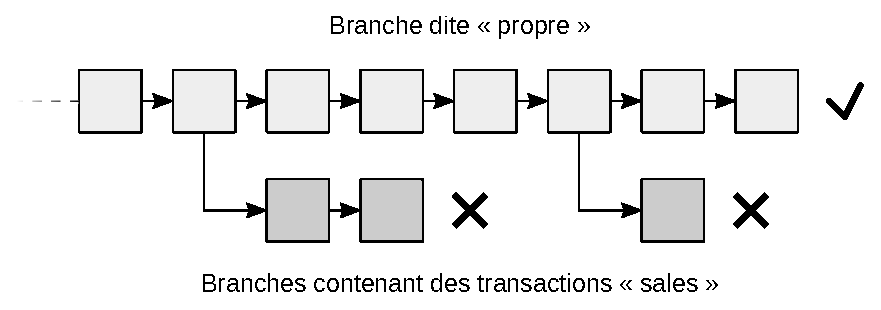
\includegraphics[scale=0.7]{img/mining-attack-censorship.eps}
  \caption{Attaque de censure active.}
  \label{fig:censorship-attack}
\end{figure}

% Cinq statégies de minage :
% - Censure : le mineur applique systématiquement la censure en rejettant les blocs contenant les transactions sales
% - Suivisme honnête : le mineur n'applique pas la censure active, applique la censure passive et prolonge la chaîne la plus longue en privilégiant le premier bloc reçu
% - Suivisme malhonnête : le mineur n'applique pas la censure active, applique la censure passive et prolonge la chaîne la plus longue en privilégiant la branche des censeurs
% - Suivisme dissident : le mineur n'applique pas la censure active, applique la censure passive et prolonge la chaîne la plus longue en privilégiant la branche des dissidents
% - Dissidence : le mineur n'applique ni la censure active, ni la censure passive, et prolonge systématiquement la branche concurrente à celle des censeurs, même si elle est plus courte

% Coût de l'attaque
Le coût d'une telle attaque peut être colossal suivant la puissance de calcul déployée sur le réseau\footnote{On a vu dans le chapitre~\ref{ch:confirmation} que le coût d'une telle attaque se chiffre en milliards de dollars sur le réseau Bitcoin principal.}. Mais ce coût serait justifié par le développement des activités illégales évitant l'impôt et le seigneuriage. En effet, comme montré dans le chapitre~\ref{ch:adversaire}, le profil-type de l'attaquant est l'État dont le pouvoir de prélèvement repose grandement sur son contrôle de la monnaie~: c'est pourquoi il se moque de réduire (voire de détruire) l'utilité de Bitcoin ce faisant.

% Intensification du conflit (guerre contre Bitcoin, marché noir)
Cette attaque hypothétique serait précédée d'une déclaration de guerre contre Bitcoin. Toute la tolérance vis-à-vis des utilisateurs disparaîtrait, et ce qui n'était pas officiel le deviendrait~: toutes les transactions qui ne sont pas explicitement autorisées seraient déclarées interdites. L'utilisation libre serait criminalisée d'une manière ou d'une autre, et le minage honnête aussi.

% Cela s'accompagnerait probablement d'une mise en avant d'une alternative~: soit une version plus conforme de Bitcoin, soit une monnaie numérique de banque centrale (MNBC), présentée comme plus sûre et moins volatile.

% Cooptation, déploiement de matériel et attaque
Ce durcissement permettrait de coopter plus largement les regroupements miniers auxquels les directives étatiques seraient transmises. L'État pourrait aussi réquisitionner ou acheter son propre matériel de hachage. En somme, il disposerait à un moment donné d'une puissance de calcul majoritaire. Une fois la puissance de calcul rassemblée, l'attaque serait mise à exécution.

% Prolongement de l'attaque
La censure active est insidieuse car il suffit que 51~\% l'applique pour qu'elle continue. Son prolongement dans le temps peut finir par constituer une nouvelle normalité. Par conséquent, les mineurs économiquement rationnels ont tout intérêt à appliquer la censure, comme l'a montré un article de Juraj Bednar sur le sujet\footnote{Juraj Bednar, \eng{Bitcoin censorship will most likely come, pt 2}, 18 novembre 2020~: \url{https://juraj.bednar.io/en/blog-en/2020/11/18/bitcoin-censorship-will-most-likely-come-pt-2/}.}. L'attaquant ne doit donc pas nécessairement disposer en permanence de la majorité du taux de hachage.

% Cas extrême, attaque Goldfinger
La confidentialité n'empêche pas la censure d'avoir lieu, mais la rend simplement plus coûteuse. Dans le cas où l'intégralité des utilisateurs refuserait de se conformer aux normes de surveillance, les censeurs devraient refuser l'ensemble des transactions et ne pas recevoir les frais correspondants. L'attaque prendrait alors la forme d'une destruction totale de l'utilité de la chaîne par le minage de blocs vides, c'est-à-dire une attaque Goldfinger. Le nom de cette dernière fait référence au principal antagoniste du film de James Bond éponyme sorti en 1964, qui souhaitait irradier le stock d'or américain sécurisé au dépôt de Fort Knox dans le but de le rendre durablement inutilisable et d'augmenter la valeur du reste de l'or\footnote{Joshua A. Kroll, Ian C. Davey, Edward W. Felten, «~\eng{The Economics of Bitcoin Mining, or Bitcoin in the Presence of Adversaries}~», in \eng{Workshop on the Economics of Information Security}, 2013~: \url{https://asset-pdf.scinapse.io/prod/2188530018/2188530018.pdf}.}.

% Censure et résistance

De ce fait, il est tout à fait possible d'exercer de la censure dans Bitcoin. Toutefois, ce n'est ni facile, ni définitif, car il existe un mécanisme au sein du protocole permettant de lutter contre ce type d'attaque~: la résistance à la censure.

\section*{Le mécanisme de résistance à la censure}
\addcontentsline{toc}{section}{Le mécanisme de résistance à la censure}

% Définition de la résistance à la censure
La résistance à la censure désigne la difficulté à entraver arbitrairement les transactions. Elle est couramment citée comme l'une des deux grandes promesses de Bitcoin~: permettre à quiconque d'envoyer des fonds à n'importe qui d'autre, quel que soit le moment, où que se trouve le destinataire dans le monde, pourvu qu'il dispose d'un accès à Internet.

% La résistance à la censure est essentielle
La résistance à la censure constitue un élément essentiel de Bitcoin. Si elle n'existait pas, le système ne pourrait tout simplement pas survivre en tant que tel~: il deviendrait un système contrôlé centralement par une autorité décidant des bonnes et des mauvaises transactions. Il devrait s'adapter, tel GoldMoney ou PayPal, ou périr, à l'instar de e-gold ou de Liberty Reserve. De plus, le pouvoir absolu sur la sélection des transactions permettrait à cette autorité d'exercer \eng{de facto} une influence irrésistible sur le protocole par le biais de l'application de soft forks (comme nous le verrons dans les chapitres \ref{ch:changement} et \ref{ch:determination}), ce qui mènerait \emph{in fine} à la destruction de la politique monétaire originelle. Sans résistance à la censure, la proposition de valeur de Bitcoin s'effondrerait.

% Pas de description par Satoshi
Cependant, cette résistance n'a jamais été décrite explicitement par Satoshi Nakamoto. Dans ses interventions, le père de Bitcoin a expliqué comment son système était sécurisé économiquement contre la double dépense, ce qui était déjà une grande évolution par rapport aux modèles décentralisés précédents. Mais il n'a en revanche pas indiqué comment le système pouvait s'opposer à la censure, c'est-à-dire au blocage partiel ou total de l'activité transactionnelle par une entité hostile. Il semblait se reposer sur la bonne volonté des mineurs «~honnêtes~», pensant même qu'il y aurait «~probablement toujours des nœuds prêts à traiter les transactions gratuitement\footnote{Satoshi Nakamoto, \eng{Bitcoin v0.1 released}, \wtime{08/01/2009 19:27:40 UTC}~: \url{https://www.metzdowd.com/pipermail/cryptography/2009-January/014994.html}.}~», cette résistance allant de soi.

% Mécanisme de résistance à la censure mis en lumière par Eric Voskuil
Le mécanisme de résistance à la censure de Bitcoin a été mis en lumière en 2018, par le développeur et auteur Eric Voskuil, qui a montré qu'il reposait de manière essentielle sur les frais de transaction\footnote{Le mécanisme de résistance à la censure a initialement été décrit par Eric Voskuil en janvier 2018~: \url{https://github.com/libbitcoin/libbitcoin-system/wiki/Other-Means-Principle/77d7556a14f89d1704f1bb97ca0aed04606363d0}. Voir aussi Eric Voskuil, «~Propriété de résistance à la censure~», in \emph{Cryptoéconomie~: Principes fondamentaux de Bitcoin}, Amazon KDP, 2022, pp.~24--25.}. Comme dans le cas de la résistance à la double dépense, la propriété de résistance à la censure n'est pas absolue mais économique~: c'est une régulation financée par les frais des transactions prohibées.

% Principe de la majorité

La sécurité minière, on le rappelle, repose sur un principe majoritaire~: la quantité de puissance de calcul contrôlée par les mineurs honnêtes doit être supérieure par rapport à celle des attaquants. L'important n'est pas que le taux de hachage de Bitcoin soit le plus haut possible~; c'est que les mineurs disposant d'une puissance de calcul non négligeable soient prêts à miner systématiquement toutes les transactions payant un montant correct de frais et à toujours construire leurs blocs à partir de la plus longue chaîne. % Pas de censue passive et pas de recoordination de chaîne

% Sécurité = activité × distribution × participation
Ainsi, cette sécurité ne dépend pas uniquement de la puissance de calcul. Elle est aussi fonction de la distribution de cette puissance de calcul et de la fraction de mineurs par rapport au reste de l'humanité\footnote{Eric Voskuil, «~Modèle de sécurité qualitatif~», in \emph{Cryptoéconomie~: Principes fondamentaux de Bitcoin}, Amazon KDP, 2022, pp.~59--62.}. En effet, un taux de hachage qui serait concentré dans les mains d'un seul mineur créerait une sécurité équivalente à celle d'un système centralisé, dépendante du mineur en question. Aussi, un réseau équitablement distribué et déployant une grande quantité de puissance de calcul aura plus de risque d'être coopté s'il comporte un petit nombre de mineurs que s'il en comporte un grand nombre.

% Compensation du risque
La solution au problème de la censure provient des mineurs dissidents, qui sont prêts à confirmer des transactions litigieuses ou décrétées comme illégales par le pouvoir. Le risque pris par ces mineurs doit alors être compensé économiquement.

% Anonymat du mineur
Le mineur dissident a besoin de rester anonyme afin de pouvoir miner dans la clandestinité. Cette possibilité est assurée par le fait que les mineurs ne sont jamais contraints de s'identifier au sein du protocole. Le signalement des blocs minés par les coopératives minières est en effet une démarche purement optionnelle et volontaire, ayant pour but de rassurer les utilisateurs (leurs clients) sur la distribution du système.

% Rôle de la création monétaire
La part du revenu du minage provenant de la création monétaire joue un rôle accessoire dans la lutte contre la censure, que cette dernière soit passive ou active. D'une part, cette partie de la récompense est la même pour tous les mineurs, ce qui fait qu'elle n'influe pas sur leur choix économique d'inclure une transaction ou non dans un bloc. D'autre part, la potentielle chute de l'utilité (et donc du revenu de minage) du système provoquée par une censure active (attaque), ne saurait empêcher l'autorité à l'origine d'arriver à ses fins. Les motivations de cette dernière sont en effet particulières~: elle ne cherche pas à réaliser un profit direct mais à contrôler, voire détruire, le système en décrétant quelles transactions sont autorisées et lesquelles ne le sont pas.

% Rôle des frais
En revanche, les frais de transaction sont, eux, essentiels au mécanisme de résistance à la censure. Par leur intégration dans le protocole, ces commissions sont chacune associées publiquement à une transaction. Ainsi, les frais luttent d'une part contre la censure passive en incitant les mineurs à confirmer les transactions, et découragent d'autre part la censure active en donnant à la branche censurée une importance économique plus grande.

% Intégration des frais
% Les frais sont intégrés au protocole. Ils sont donc généralement l'association directe avec la transaction. Ceux-ci peuvent être payés directement par les clients qui envoient les transactions, ou ils peuvent être indirectement pris en charge par les commerçants au moyen de l'application d'une réduction sur le prix des biens vendus.

% Attaque
Dans le cas d'une attaque de censure active, les censeurs acquièrent plus de la moitié de la puissance de calcul du réseau et rejettent ouvertement un groupe de transactions défini (par une liste noire par exemple) en refusant les blocs qui contiendrait l'une d'entre elles. La chaîne des censeurs est considérée par les nœuds honnêtes comme la chaîne correcte car elle est plus longue.

% Réaction
C'est dans ce contexte que le mécanisme des frais intervient. Les initiateurs des transactions censurées, voyant que leurs transactions ne sont pas confirmées, augmentent leurs commissions. C'est un comportement naturel que l'on observe déjà lors des périodes de congestion du réseau, comme au sommet de la bulle de 2017, lorsque les frais médians par transaction ont dépassé les 30~\$\pagenote{«~lorsque les frais médians par transaction ont dépassé les 30~\$~»~: \url{https://bitinfocharts.com/comparison/bitcoin-median_transaction_fee.html\#alltime}.}. En outre, il est logique de payer une grande quantité de frais pour transférer de fortes sommes, celles-ci étant plus à risque que les petits transferts\footnote{Dans Bitcoin, les frais sont aujourd'hui payés proportionnellement à la charge des données (taille ou poids de la transaction). Cependant, la menace de plus en plus claire de la censure pourrait pousser les utilisateurs à payer des frais proportionnels au montant transféré comme cela se fait dans le domaine financier en général.}.

% Supplément de frais
Cette augmentation crée un supplément de frais, qui constitue la différence entre les frais de toutes les transactions et ceux des transactions non autorisées qui se retrouvent dans les mempools des nœuds honnêtes. C'est ce supplément (et ce supplément uniquement) qui incite les mineurs dissidents à déployer plus de puissance de calcul au cours du temps~: plus l'économie supprimée est importante, plus le différentiel de puissance de calcul résultant est grand.

% Riposte
Les mineurs dissidents se coordonnent en privé ou par la voie d'un signalement pour planifier une riposte. Une fois que la puissance de calcul est jugée suffisante, ils se mettent à confirmer les transactions censurées. Puisque leur puissance de calcul est majoritaire, leur chaîne devient la plus longue et la chaîne des censeurs est invalidée. De cette manière, la censure est vaincue, du moins jusqu'à une nouvelle offensive de l'ennemi.

% Mécanisme ancré dans le protocole
Ainsi, le mécanisme de résistance à la censure est ancré profondément dans le protocole. La preuve de travail, le caractère anonyme du minage, le système de frais intégré~: ce sont autant d'éléments permettant de coordonner un marché des frais afin de repousser les censeurs. Il est impossible d'estimer quelle serait la part de l'économie censurée, l'envergure de l'attaque étatique ou le montant de frais que les utilisateurs seraient prêts à payer, de sorte qu'on ne peut pas garantir l'incensurabilité de Bitcoin. Mais le mécanisme n'en est pas moins fonctionnel.

% Négligence du rôle des frais de transactions
Il est à noter que le rôle des frais de transaction, explicité en 2018 par Eric Voskuil, a été négligé par certains protocoles cryptoéconomiques. C'est en particulier le cas d'Ethereum qui a fait le choix de brûler une partie des frais du réseau dans le but de rendre l'éther déflationniste au sens monétaire avec l'activation de l'EIP-1559 en août 2021\pagenote{«~l'activation de l'EIP-1559 en août 2021~»~: Ludovic Lars, \emph{Ethereum face à une catastrophe annoncée~? Censure et volatilité~: l'EIP-1559, le cauchemar des mineurs}, 15 juillet 2021~: \url{https://journalducoin.com/analyses/eip-1559-changement-nefaste-ethereum/}.}. La communauté d'Ethereum a également choisi de passer en preuve d'enjeu en septembre 2022, ce qui constitue un autre pas vers l'acceptation de la censure comme nous l'expliquerons plus bas.

\vspace{-1em}
\section*{L'importance de la confidentialité}
\addcontentsline{toc}{section}{L'importance de la confidentialité}

La censure financière est étroitement apparentée à la surveillance des transactions. Cette dernière permet en effet d'affiner la sélection des transferts et d'exercer un pouvoir subtil sur l'économie, sans brusquer les personnes les plus dociles. La chose vaut pour le monde bancaire comme nous l'avons constaté, mais elle vaut aussi pour Bitcoin.

% --- Deux manières de protéger sa richesse ---

% Défense physique
Il existe deux manières de protéger sa richesse et sa liberté~: par la force physique et par la dissimulation. La première méthode consiste à se prémunir contre le vol directement en défendant soi-même ses biens (si besoin à l'aide d'une arme à feu), ou bien indirectement par le recours aux services de police étatiques ou aux services de protection privés (gardes du corps, quartiers sécurisés, agence de protection), très prisés des personnes très fortunées. Cette méthode est importante et utile contre les criminels communs, mais elle est relativement inefficace contre la puissance dominante locale dont nous sommes à la merci -- l'État.

% Défense par dissimulation
C'est pourquoi les individus ont plus souvent recours à la seconde méthode, qui consiste à dissimuler leur richesse pour ne pas qu'autrui en ait connaissance et puisse s'en emparer directement. Cela permet de dissuader le voleur usant la menace de violence d'aller plus loin~: il pourrait nous interroger pour savoir où se trouve notre richesse, mais cette action représenterait un coût supplémentaire (proportionnel à notre refus de lui livrer cette information) qui freinerait sa recherche.

% Définition de la confidentialité
Cette méthode est directement liée à la confidentialité (aussi appelée \eng{privacy} ou protection de la vie privée) qui est le fait de réserver des informations à un petit nombre de personnes déterminées. La confidentialité est distincte du secret dans le sens où la personne peut choisir de révéler sélectivement des informations (confidence). Dans le contexte financier, il s'agit généralement de faire en sorte que les détails d'une transaction ne soient connus que des participants.

% La confidentialité crée la liberté individuelle
La confidentialité forme la base de la liberté individuelle dans la société et constitue une caractéristique essentielle pour tout le monde. Elle sert en effet à \emph{créer une asymétrie} entre le faible et le fort, entre l'individu et l'État, de sorte que ce dernier ne puisse pas empiéter absolument sur les droits du premier. L'État veut vous persuader du contraire, en vous disant que vous n'avez rien à craindre si vous n'avez rien à cacher\footnote{«~Je dis que quiconque tremble en ce moment est coupable~; car jamais l'innocence ne redoute la surveillance publique.~» -- Maximilien de Robespierre, \emph{Discours du 11 germinal, an II}, 31 mars 1794.}, mais il n'y a rien d'historiquement plus faux, comme l'ont montré les exemples des totalitarismes du \textsc{xx}\ieme{}~siècle.

% --- Lien entre résistance à la censure et confidentialité ---

De ce fait, puisque la censure financière est issue de l'initiative étatique, la résistance à la censure est en général intrinsèquement liée à la confidentialité.

% Confidentialité => résistance à la censure
D'une part, la résistance à la censure de l'utilisateur individuel repose sur la confidentialité du système. Si l'État connaît toutes les transactions, il peut sanctionner l'utilisateur pour avoir effectué une transaction non autorisée, quand bien même celle-ci serait confirmée par le réseau. Certains promoteurs de BTC mettent en avant la transparence du protocole, en la présentant comme un avantage par rapport aux systèmes bancaires opaques, en insistant sur le pseudonymat et en réservant la propriété d'anonymat aux «~cryptomonnaies confidentielles~» comme Monero. Mais il s'agit d'une mécompréhension du rôle de cette transparence~: les données dans Bitcoin sont publiques dans le but unique d'assurer le consensus et l'audit, et Monero ne fait qu'implémenter un compromis différent sur le degré de transparence des transactions.

% Résistance à la censure => confidentialité
D'autre part, la confidentialité de l'utilisateur dépend de la résistance à la censure du système. En effet, si l'État dispose d'un contrôle total sur la sélection des transactions, alors il peut choisir de ne confirmer que les transactions qui dévoilent l'identité de l'expéditeur et celle du destinataire. Cette dépendance est souvent remise en question par certains partisans de Monero qui estiment que la confidentialité par défaut du système protège les utilisateurs de la censure, considérant que l'État ne peut pas censurer une transaction qu'il ne connaît pas. Néanmoins, cette vision est plutôt naïve car les utilisateurs ont la possibilité technique de révéler les informations relatives à leurs adresses aux organismes de surveillance\footnote{Dans Monero et dans les systèmes apparentés, la révélation des transactions liées à une adresse se fait par l'intermédiaire d'une clé privée d'inspection (\eng{private view key}).}~; la seule barrière à cela est le coût supplémentaire qu'une telle surveillance représente. % C'est pour cette raison qu'un État pourrait choisir de refuser toute transaction non transparente. La résistance à la censure dépend aussi du coût de l'attaque, qui serait beaucoup moins coûteuse à réaliser dans le cas de Monero, probablement 200 fois moins que sur BTC (mars 2023).

% Interdépendance de la confidentialité et de la résistance à la censure
La confidentialité et la résistance à la censure sont donc interdépendantes dans Bitcoin. Sans confidentialité, il n'y a pas de résistance à la censure individuelle~; et sans résistance à la censure, il n'y a pas de confidentialité individuelle. C'est pour cette raison que la surveillance généralisée, loin d'être anodine, constitue un problème majeur.

% État des lieux de la surveillance des intermédiaires
La surveillance s'est étendue dans Bitcoin au cours de son développement économique par la réglementation des intermédiaires financiers. Les plateformes de change entre monnaies traditionnelles et cryptomonnaies ont été progressivement contraintes d'appliquer des normes de connaissance du client (KYC) et de lutte contre le blanchiment (AML) similaires au système bancaire classique. Cette récupération d'informations s'est accompagnée de l'émergence de sociétés d'analyses de chaîne, telles que Chainalysis ou CipherTrace, qui croisent les données d'identification avec les évènements de la chaîne de blocs de façon à en dégager une interprétation probable, et qui fournissent les résultats à leurs clients qui sont les agences étatiques, les institutions financières et les grandes entreprises du domaine. En outre, l'étau est encore en train de se resserrer, avec l'apparition d'une version modifiée de la «~règle du voyage~» (\eng{Travel Rule}), recommandée par le GAFI et déjà imposée par la FINMA suisse, qui consiste pour un intermédiaire à vérifier systématiquement l'adresse de retrait du client\footnote{Dans le monde bancaire, la \eng{Travel Rule} a originellement été promulguée par le FinCEN étasunien en 1996 (voir 31 CFR 103.33(g)). Elle exige que toutes les institutions financières transmettent des informations sur les expéditeurs à l'institution financière suivante lors de certains transferts de fonds. Dans le cas de Bitcoin et des cryptomonnaies, il s'agit d'émuler ce voyage en considérant que les utilisateurs sont des institutions financières lorsqu'ils réalisent des transactions souveraines. Le GAFI a ajouté le transfert d'«~actifs virtuels~» à ses recommandations en juin 2019, notamment en ce qui concerne la recommandation 16. Cette règle du voyage cryptomonétaire pourrait être appliquée par l'intégration dans les portefeuilles du protocole de preuve de propriété d'adresse (AOPP) proposé en janvier 2022.}\pagenote{«~l'apparition d'une version modifiée de la "règle du voyage", recommandée par le GAFI et déjà imposée par la FINMA suisse~»~: \url{https://www.fincen.gov/sites/default/files/advisory/advissu7.pdf} -- Recommandation 16 du GAFI, mise à jour en juin 2019 pour inclure le transferts d'actifs virtuels~: \url{https://www.fatf-gafi.org/fr/publications/Recommandationsgafi/Recommandations-gafi.html}. -- \url{https://www.finma.ch/en/news/2019/08/20190826-mm-kryptogwg/} -- \url{https://aopp.group/}.}.

% Lutte contre la surveillance
Cette évolution crée une réelle menace sur Bitcoin en général. C'est pourquoi il se forme en face une résistance visant à déjouer la surveillance, notamment par l'intermédiaire de techniques d'amélioration de la confidentialité. C'est le cas par exemple du mélange de pièces, ou CoinJoin, qui permet de brouiller les pistes. C'est aussi le cas des méthodes intégrées dans Monero. Nous développerons cet aspect dans le chapitre~\ref{ch:rouages}. % Mais ces méthodes doivent être utilisées, et elles doivent rester à jour de l'avancée de la surveillance.

% Importance de la confidentialité
Ainsi, la confidentialité est essentielle pour préserver sa richesse et son autonomie. On ne peut pas être réellement libre sans protéger sa vie privée. Comme l'écrivait le fabuliste Florian~: «~Pour vivre heureux vivons cachés\footnote{Jean-Pierre Claris de Florian, «~Le Grillon~», in \emph{Fables de Florian}, 1793.}.~»

\section*{Les interventions humaines dans le consensus}
\addcontentsline{toc}{section}{Les interventions humaines dans le consensus}

La possibilité de censure dans Bitcoin provoque généralement une volonté de trouver une solution, s'inscrivant dans la démarche d'ingénieur qui caractérise les amateurs de cryptomonnaie. Beaucoup de personnes sont en effet séduites par une alternative à la régulation par les frais~: l'intervention humaine directe sur la chaîne. Celle-ci consiste à recourir au «~consensus social\pagenote{«~consensus social~»~: Arthur Breitman parlait de \eng{social consensus} dès août 2014 dans la première description formelle de Tezos. -- Arthur Breitman, \eng{Tezos: A Self-Amending Crypto-Ledger}, 3 août 2014~: \url{https://tezos.com/position-paper.pdf}.}~», c'est-à-dire au mécanisme de détermination du protocole. Deux idées de ce type semblent avoir un certain succès~: l'UASF anti-censure et l'UAHF de changement de preuve de travail. Il s'agit cependant d'une tentation dangereuse comme nous allons essayer de le montrer.

% Lorsqu'on parle de la possibilité de censure, une autre alternative a tendance à séduire les personnes qui n'ont pas suffisamment creusé la question~: celle d'intervenir socialement sur la chaîne. Il s'agit d'avoir recours au «~consensus social\footnote{Pour reprendre l'expression d'Arthur Breitman utilisée dans la première description formelle de Tezos en août 2014. -- Arthur Breitman, \eng{Tezos: A Self-Amending Crypto-Ledger}, 3 août 2014~: \url{https://tezos.com/position-paper.pdf}.}~», c'est-à-dire le mécanisme de détermination du protocole.

% --- UASF anti-censure ---

La première idée est de rejeter la censure en invalidant la branche des censeurs partiellement ou totalement, c'est-à-dire en portant atteinte au principe de la chaîne la plus longue. Le rejet peut se faire en rendant les blocs de la chaîne des censeurs invalides ou en imposant la validité de la chaîne concurrente par un point de contrôle temporaire. Une telle mesure constitue un soft fork (à savoir une restriction des règles de consensus) et doit être activée par les utilisateurs à un horodatage ou à une hauteur de bloc donné, d'où le fait qu'on la désigne comme un \eng{User Activated Soft Fork} (UASF). Elle provoque une scission car elle n'est pas, dans le cas précis de la censure, soutenue par la majorité de la puissance de calcul.

% Vitalik
L'idée d'invalider la censure par consensus social était déjà évoquée par Vitalik Buterin en 2016 dans le cas de la preuve d'enjeu~:

\begin{quote}
«~\emph{Sur des échelles de temps moyennes à longues, les humains sont assez bons pour le consensus.} Même si un attaquant avait accès à une puissance de hachage illimitée, et qu'il parvenait à réaliser une attaque des 51~\% contre une chaîne de blocs majeure en inversant ne serait-ce que le dernier mois d'histoire, il aurait beaucoup plus de mal à convaincre la communauté de la légitimité de la nouvelle chaîne. Il faudrait qu'il subvertisse les explorateurs de blocs, tous les membres de confiance de la communauté, le New York Times, archive.org et de nombreuses autres sources sur Internet ; en somme, qu'il convainque le monde que sa nouvelle chaîne est celle qui est apparue en premier [...]. \emph{Ces considérations sociales sont ce qui protège finalement toute chaîne de blocs à long terme}, que la communauté de cette chaîne de blocs l'admette ou non (notez que Bitcoin Core admet cette primauté de la couche sociale)\footnote{Vitalik Buterin, \eng{A Proof of Stake Design Philosophy}, 30 décembre 2016~: \url{https://medium.com/@VitalikButerin/a-proof-of-stake-design-philosophy-506585978d51}.}.~»
\end{quote}

% "On medium to long time scales, humans are quite good at consensus. Even if an adversary had access to unlimited hashing power, and came out with a 51\% attack of any major blockchain that reverted even the last month of history, convincing the community that this chain is legitimate is much harder than just outrunning the main chain's hashpower. They would need to subvert block explorers, every trusted member in the community, the New York Times, archive.org, and many other sources on the internet; all in all, convincing the world that the new attack chain is the one that came first in the information technology-dense 21st century is about as hard as convincing the world that the US moon landings never happened. These social considerations are what ultimately protect any blockchain in the long term, regardless of whether or not the blockchain's community admits it (note that Bitcoin Core does admit this primacy of the social layer).
%
% However, a blockchain protected by social consensus alone would be far too inefficient and slow, and too easy for disagreements to continue without end (though despite all difficulties, it has happened); hence, economic consensus serves an extremely important role in protecting liveness and safety properties in the short term."

% Invalidation des blocs des censeurs
Cette mesure peut être mise en place par une invalidation directe mais celle-ci n'est facile à implémenter que si les censeurs marquent leurs blocs d'une manière ou d'une autre\pagenote{«~invalidation directe~»~: Cette méthode peut par exemple être mise en place dans l'esprit de l'\eng{User Resisted Soft Fork} proposé par Michael Folkson en avril 2022 en réaction à la menace d'activation de la mise à niveau \longstring{OP\_CHECKTEMPLATEVERIFY}. -- Michael Folkson, \eng{[bitcoin-dev] User Resisted Soft Fork for CTV}, \wtime{21/04/2022 16:45:20 UTC}~: \url{https://lists.linuxfoundation.org/pipermail/bitcoin-dev/2022-April/020262.html}.}. Cela a été réalisé par Bitcoin ABC le 1\ier{} décembre 2020 sur sa chaîne nouvellement créée pour contrer la censure active d'un mineur mécontent de la scission avec Bitcoin Cash\footnote{Un seul bloc (le bloc 662~687 d'identifiant \longstring{00000000000000000709b858a6a0c8610e604e77072ef4407763afb0780ce712}) de l'attaquant a été invalidé, faisant que 172 blocs ont été mis de côté, et que la chaîne non censurée est devenue la chaîne correcte. -- Nikita Zhavoronkov sur Twitter, \wtime{01/12/2020 21:59 UTC}~: \url{https://twitter.com/nikzh/status/1333893457920876550}.}.

% Point de contrôle
Il est aussi possible d'inclure un point de contrôle (\eng{checkpoint}) dans le protocole. Un point de contrôle est un bloc considéré comme valide par défaut. Ce mécanisme a été implémenté dans le logiciel de Bitcoin dès juillet 2010 dans le but d'éviter une recoordination de chaîne\pagenote{«~implémenté dans le logiciel de Bitcoin dès juillet 2010~»~: Satoshi Nakamoto, \eng{Bitcoin 0.3.2 released}, \wtime{17/07/2010 21:35:51 UTC}~: \url{https://bitcointalk.org/index.php?topic=437.msg3807\#msg3807}.} et certains de ces points de contrôle sont encore présents dans Bitcoin Core\footnote{Le point de contrôle le plus récent est celui du bloc 295~000 miné le 9 avril 2014 (au même moment de l'arrivée de Wladimir van der Laan au poste de mainteneur principal) et ayant pour identifiant \longstring{00000000000000004d9b4ef50f0f9d686fd69db2e03af35a100370c64632a983}. Voir le fichier \longstring{chainparams.cpp} dans Bitcoin Core.}\pagenote{«~certains de ces points de contrôle sont encore présents dans Bitcoin Core~»~: \url{https://github.com/bitcoin/bitcoin/blob/24.x/src/chainparams.cpp\#L148-L164}.}. Dans cette logique, il suffit d'imposer un bloc comme obligatoire pour invalider la chaîne des censeurs. Cela a été réalisé par Bitcoin SV en août 2021, qui subissait alors une censure active\footnote{BSV Association sur Twitter, \wtime{03/09/2021 21:17 UTC}~: \url{https://twitter.com/BitcoinAssn/status/1422668065024663554}.}.

% Efficacité de l'intervention humaine
Toutefois, même si ce type de recours peut effectivement fonctionner de manière ponctuelle et temporaire, il ne constitue en rien un mécanisme robuste de résistance à la censure. En effet, il crée beaucoup trop d'instabilité en faisant en dernier lieu reposer le consensus sur l'accord social. Il offre ainsi la possibilité pour une puissance hostile de déstabiliser durablement le système en semant la zizanie dans la communauté (notamment par la pression exercée sur les relais d'opinion) et en créant par là des scissions multiples impossibles à départager par un facteur objectif.

% Pourquoi l'UASF anti-censure est une mauvaise idée

L'intervention directe de l'accord social dans la confirmation des transactions est par conséquent une très mauvaise idée. Même dans les cas où les participants sont d'accord pour dire qu'un tel évènement est indésirable, ils sont souvent en total désaccord sur la manière de traiter le problème, ainsi qu'on l'a observé lors de la scission entre Ethereum et Ethereum Classic. Les être humains sont capables de se mettre d'accord à long terme, comme le témoigne la convergence vers un petit nombre de langues, de religions, de monnaies, etc. Néanmoins, à court terme ce n'est très certainement pas le cas. D'où le recours au mécanisme de consensus automatisé qu'est le minage.

% --- UAHF de changement de preuve de travail de preuve de travail ---

Une autre mesure proposée, moins subjective mais plus perturbatrice, est la modification de la fonction de preuve de travail. Celle-ci permet de faire cesser l'attaque à court terme puisqu'elle rend le matériel spécialisé des censeurs obsolète, leur faisant supporter une lourde perte au passage. Il s'agit d'un hard fork (à savoir une modification incompatible des règles de consensus) qui doit être activé par les utilisateurs à un horodatage ou à une hauteur de bloc donné, c'est-à-dire un \eng{User Activated Hard Fork} (UAHF). Cette option extrême a été soutenue par les développeurs Luke-Jr et Gregory Maxwell lors de la guerre des blocs en 2015 -- 2016\pagenote{«~soutenue par les développeurs Luke-Jr et Gregory Maxwell~»~: \url{https://www.reddit.com/r/Bitcoin/comments/3fg0jw/could_a_cartel_of_pool_operators_collude_to/ctoat0d/}~;\url{https://www.reddit.com/r/bitcoinxt/comments/41pbmf/maxwell_considers_changing_the_pow_algorithm_in/}.}. Elle a également été défendue par le développeur en chef de Bitcoin ABC Amaury Séchet en novembre 2018 qui l'a qualifiée d'«~option nucléaire [...] de dernier recours\footnote{Amaury Séchet (deadalnix) sur Twitter, \wtime{12/11/2018 11:42 UTC}~: \url{https://twitter.com/deadalnix/status/1061947426096009216}.}~».

% Pourquoi le hard fork de changement de preuve de travail est une mauvaise idée
De même que dans le cas de l'invalidation de la censure par intervention sociale, il s'agit d'une mesure plus néfaste à long terme que le statu quo. Premièrement, la perte subie par les censeurs est aussi encaissée par les mineurs honnêtes et dissidents. Deuxièmement, l'économie est répartie entre deux chaînes distinctes, réduisant l'utilité monétaire totale. Troisièmement, le coût d'une attaque est drastiquement réduit à court terme. Quatrièmement, les mineurs perdent confiance dans le protocole et doivent s'assurer contre le risque d'un nouveau changement, réhaussant le coût de la sécurité minière par rapport au coût de l'attaque. Et cinquièmement, la nouvelle distribution du minage n'est pas forcément meilleure que l'ancienne, les gros mineurs pouvant déployer du capital plus facilement.

% Effet néfaste de l'intervention humaine
De manière générale, l'intervention humaine à court terme est loin d'être désirable. Si la chaîne subit une attaque minière, il est probable qu'elle soit aussi attaquée au niveau social. Les interventions ont ainsi toutes les chances de se multiplier, faisant sombrer la chaîne dans une spirale de scissions et la menant à l'insignifiance économique. Le cas de Bitcoin Cash est le plus éclairant~: en raison de hard forks programmés tous les six mois, la chaîne a subi deux scissions majeures après sa séparation avec Bitcoin-BTC (en 2018 avec BSV et en 2020 avec XEC), ce qui a mené l'ensemble à être valorisé à moins de 1~\% de la valeur agrégée du BTC. En outre, si ce caractère néfaste est valable pour les cryptomonnaies en construction, qui peuvent se permettre ces interventions en raison de la petitesse et de l'homogénéité de leur économie, elle l'est d'autant plus pour une version mature de Bitcoin qui soutiendrait une économie plus grande et plus diversifiée.

\section*{Les variantes des consensus par preuve de travail}
\addcontentsline{toc}{section}{Les variantes des consensus par preuve de travail}

% Alternatives, variantes
Le risque de censure a également inspiré le développement d'algorithmes de consensus alternatifs à celui de Bitcoin. L'alternative la plus connue est la preuve d'enjeu, qui sera décrite dans la section suivante. Les autres alternatives sont des variantes de l'algorithme de Nakamoto par preuve de travail, dont les trois principales sont le minage combiné, la preuve d'espace et la finalisation anticipée. % protection contre la recoordination profonde, "checkpoints automatiques"

% --- Minage combiné ---

La première proposition est le minage combiné\pagenote{«~le minage combiné~»~: Aljosha Judmayer, Alexei Zamyatin, Nicholas Stifter, Artemios G.  Voyiatzis, Edgar Weippl, \eng{Merged Mining: Curse of Cure?}, 22 août 2017~: \url{https://eprint.iacr.org/2017/791}.}. Le minage combiné, ou \eng{merge mining} en anglais, est l'action de miner plusieurs chaînes en simultané par la réutilisation du travail fourni sur une chaîne mère pour la validation des chaînes filles ou auxiliaires.

Le procédé a été décrit par Satoshi Nakamoto en décembre 2010, dans un message concernant BitDNS, le projet de système distribué de noms de domaine à l'origine de Namecoin. Le créateur de Bitcoin écrivait ainsi sur le forum~:

\begin{quote}
«~Je pense qu'il serait possible que BitDNS forme un réseau complètement séparé et possède une chaîne de blocs distincte, tout en partageant la puissance de calcul avec Bitcoin. Le seul chevauchement consisterait à faire en sorte que les mineurs puissent rechercher des preuves de travail pour les deux réseaux simultanément.

Les réseaux n'auraient besoin d'aucune coordination. Les mineurs adhéreraient aux deux réseaux en parallèle. Ils scanneraient SHA de telle sorte que s'ils obtenaient un résultat, ils pourraient résoudre les deux en même temps. Une solution pourrait concerner un seul des réseaux si l'un d'eux présentait une difficulté moindre.

Je pense qu'un mineur externe pourrait appeler getwork sur les deux programmes et combiner le travail. Peut-être appeler Bitcoin, en tirer un travail, le remettre à getwork sur BitDNS pour le combiner en un travail commun.

Plutôt que de fragmenter l'ensemble, les réseaux partageraient et augmenteraient la puissance de calcul totale de chacun. Cela résoudrait le problème des réseaux multiples, qui constituent un danger les uns pour les autres si la puissance de calcul disponible se concentre sur l'un d'entre eux. Au lieu de cela, tous les réseaux du monde partageraient la puissance de calcul combinée, augmentant ainsi la puissance totale. Il serait plus facile pour les petits réseaux de se lancer en puisant dans une base existante de mineurs\footnote{Satoshi Nakamoto, \eng{Re: BitDNS and Generalizing Bitcoin}, \wtime{09/12/2010 21:02:42 UTC}~: \url{https://bitcointalk.org/index.php?topic=1790.msg28696\#msg28696}.}.~»
\end{quote}

% "I think it would be possible for BitDNS to be a completely separate network and separate block chain, yet share CPU power with Bitcoin.  The only overlap is to make it so miners can search for proof-of-work for both networks simultaneously.
%
% The networks wouldn't need any coordination.  Miners would subscribe to both networks in parallel.  They would scan SHA such that if they get a hit, they potentially solve both at once.  A solution may be for just one of the networks if one network has a lower difficulty.
%
% I think an external miner could call getwork on both programs and combine the work.  Maybe call Bitcoin, get work from it, hand it to BitDNS getwork to combine into a combined work.
%
% Instead of fragmentation, networks share and augment each other's total CPU power.  This would solve the problem that if there are multiple networks, they are a danger to each other if the available CPU power gangs up on one.  Instead, all networks in the world would share combined CPU power, increasing the total strength.  It would make it easier for small networks to get started by tapping into a ready base of miners."

% Preuves de travail auxiliaires
Le minage combiné consiste à réutiliser des preuves de travail partielles d'une chaîne mère comme des preuves de travail valides sur une chaîne fille. Ces preuves de travail, dites «~auxiliaires~» et abrégées en AuxPOW, sont des sous-produits du minage de la chaîne mère, et ne nécessitent pas de dépense d'énergie supplémentaire. La seule charge imposée par le minage combiné est la gestion de la chaîne fille.

% Récompense des mineurs de la chaîne fille
Les mineurs de la chaîne fille reçoivent des récompenses supplémentaires qui sont constituées de la création monétaire locale (si la chaîne utilise une nouvelle unité de compte) et des frais de transaction. Les mineurs de la chaîne mère sont donc incités à tirer profit de cette nouvelle manne. La chaîne fille peut de ce fait disposer d'un taux de hachage conséquent assez rapidement.

% Applications : facilitation de l'amorçage, chaîne latérale
Le minage combiné a été mis en avant comme une méthode permettant de faciliter l'amorçage d'une nouvelle cryptomonnaie, en bénéficiant de l'industrie minière établie. Ce type d'algorithme de consensus a ainsi été mis en place sur Namecoin par rapport à Bitcoin et sur Dogecoin par rapport à Litecoin. Il a aussi été suggéré comme mécanisme de synchronisation des chaînes latérales. Il est ainsi implémenté de manière hybride dans RSK. Il est plus largement envisagé par Paul Sztorc dans sa proposition de Drivechain (voir chapitre~\ref{ch:scalabilite}).

% Sécurité incertaine
Cependant, l'apport en sécurité du minage combiné par rapport au minage classique est relativement faible. Le procédé permet d'augmenter le nombre d'acteurs impliqués et de restreindre les attaquants possibles (ceux-ci devant être des mineurs de la chaîne principale), mais il ne modifie pas le coût de l'attaque, qui dépend du revenu minier de cette chaîne et, dans le cas de la censure, des frais de transaction.

% Exemple du Coiledcoin
Une illustration éclatante de ce fait est l'exemple de Coiledcoin (CLC), une cryptomonnaie alternative créée en janvier 2012 qui a subi une attaque de censure fatale peu de temps après son lancement. L'attaque a été réalisée par le développeur de Bitcoin Luke-Jr par le biais de sa coopérative de minage, Eligius, sans qu'il n'en informe les hacheurs. Dans son message d'explication, il précisait qu'aucun membre de la coopérative n'avait subi de perte, le coût étant surtout le temps qu'il avait passé à configurer le logiciel\footnote{Luke-Jr, \eng{Re: [DEAD] Coiledcoin - yet another cryptocurrency, but with OP\_EVAL!}, \wtime{06/01/2012 18:56:03 UTC}~: \url{https://bitcointalk.org/index.php?topic=56675.msg678006\#msg678006}.}.

% Effets sur la sécurité de la chaîne mère
Le minage combiné a deux effets sur la sécurité minière de la chaîne mère. D'une part, il augmente artificiellement la puissance de calcul déployée pour miner des blocs, ce qui paraît bénéfique de prime abord. Cependant, cette hausse artificielle n'agit en rien contre la censure des transactions. D'autre part, le minage combiné entraîne une centralisation de l'activité minière, en raison de la charge que représente la gestion des chaînes auxiliaires~: si les chaînes auxiliaires deviennent importantes économiquement, les mineurs de la chaîne mère n'ont d'autre choix que de les miner pour rester rentables.

% Autre variante~: «~preuve de preuve~», notamment mise en place de manière hybride par le projet Veriblock de Jeff Garzik, qui consiste à placer une représentation de l'état de la chaîne sur une chaîne de blocs parente telle que celle de BTC. Komodo's Delayed Proof Of Work.

% --- Preuve d'espace ---

La deuxième alternative est la preuve d'espace\pagenote{«~la preuve d'espace~»~: Stefan Dziembowski, Sebastian Faust, Vladimir Kolmogorov, Krzysztof Pietrzak, \eng{Proofs of Space}, 2013~: \url{https://eprint.iacr.org/2013/796}.} (de l'anglais \eng{proof of space}), parfois aussi appelée preuve de capacité ou preuve de stockage, qui se base, non pas sur le calcul informatique, mais sur la capacité à garder des données en mémoire. La ressource n'est plus la puissance de calcul, mais l'espace disque.

% Résistance aux ASIC : scrypt, ETHash, RandomX
Cette idée a été partiellement incluse dans certains algorithmes hybrides de preuve de travail, dans le but de décourager le développement de matériel spécialisé (ASIC) et de favoriser le minage par processeurs accessibles au grand public (CPU et GPU). C'est le cas de la fonction scrypt (ou S-Crypt), une fonction de dérivation de clé coûteuse en mémoire adaptée par le mineur ArtForz pour être intégrée au sein de Tenebrix en septembre 2011\pagenote{«~intégrée au sein de Tenebrix en septembre 2011~»~: Lolcust, \eng{[ANNOUNCE] Tenebrix, a CPU-friendly, GPU-hostile cryptocurrency}, \wtime{26/09/2011 00:09:44 UTC}~: \url{https://bitcointalk.org/index.php?topic=45667.msg544675\#msg544675}.}. Celle-ci a été héritée plus tard par Litecoin\pagenote{«~héritée plus tard par Litecoin~»~: Charlie Lee, \eng{Re: [ANN] Litecoin - a lite version of Bitcoin. Be ready when is launches!}, \wtime{09/10/2011 06:14:28 UTC}~: \url{https://bitcointalk.org/index.php?topic=47417.msg564414\#msg564414}.}. C'est également le cas de l'ancienne fonction de minage d'Ethereum utilisé entre 2015 et 2022, ETHash, qui est une variante de l'algorithme Dagger-Hashimoto et qui rend le calcul de la preuve plus coûteux en mémoire par la nécessité de stocker un graphe acyclique orienté de plusieurs gigaoctets\pagenote{«~ETHash~»~: \url{https://ethereum.org/en/developers/docs/consensus-mechanisms/pow/mining-algorithms/ethash/}.}. Ethereum utilisait de plus une version modifiée de l'algorithme de Nakamoto, GHOST, qui avait pour intérêt de sélectionner la chaîne la plus lourde en prenant en compte les blocs orphelins\pagenote{«~GHOST~»~: \eng{Ethereum Whitepaper}, consulté le 11 mars 2023~: \url{https://ethereum.org/en/whitepaper/\#modified-ghost-implementation}.}. Depuis novembre 2020, Ethereum Classic utilise une variante de ETHash nommée ETCHash\pagenote{«~ETCHash~»~: \url{https://github.com/eth-classic/etchash/blob/main/README.md}.}. Un dernier exemple est l'algorithme RandomX, actif sur Monero depuis 2019, qui est conçu spécialement pour favoriser le minage par CPU\pagenote{«~RandomX~»~: \url{https://github.com/tevador/RandomX}.}.

% Preuve d'espace
Au-delà des fonctions de preuve de travail coûteuses en mémoire, il existe des algorithmes de preuve d'espace pure. C'est en pratique le cas du système Chia Network, projet de Bram Cohen, qui se base sur les «~preuves d'espace et de temps~» pour déterminer la chaîne correcte\pagenote{«~Chia Network~»~: Ludovic Lars, \eng{Face à la preuve de travail de Bitcoin, la preuve d'espace, une fausse solution écologique}, 19 mai 2021~: \url{https://journalducoin.com/analyses/preuve-espace-fausse-solution-ecologique/}.}.

% Apport supposé de ces algorithmes
Ces algorithmes fondés à des degrés divers sur la mémoire informatique sont censés être plus résistants à la censure en facilitant la participation du grand public et en améliorant de ce fait la distribution de la validation. Mais ils ne font que déplacer le problème. Ce qu'il faut comprendre avec la preuve d'espace, c'est qu'il s'agit de dépenser de l'énergie extérieure d'une autre manière. La preuve d'espace est une preuve de travail déguisée~: elle revient en fin de compte à effectuer une autre forme de travail, qui peut être optimisée. Cette optimisation peut avoir lieu tant au niveau de la conception du matériel (ASIC) qu'au niveau de l'organisation industrielle (économie d'échelle), ce qui fait que les pressions centralisatrices ne disparaissent pas complètement. Tout ce qu'on peut espérer, c'est de rapprocher l'efficacité du matériel spécialisé de celle d'un outil utilisé par tous, comme ce qui est fait par RandomX avec le CPU.

% --- Finalisation anticipée des blocs ---

La troisième alternative est la finalisation anticipée des blocs. Celle-ci consiste à mettre en place des points de contrôle mobiles au sein du protocole, de façon à considérer comme final tout bloc qui se trouverait en dessous d'une certaine profondeur. Vitalik Buterin parle de «~subjectivité faible\footnote{Vitalik Buterin, \eng{Proof of Stake: How I Learned to Love Weak Subjectivity}, 25 novembre 2014~: \url{https://blog.ethereum.org/2014/11/25/proof-stake-learned-love-weak-subjectivity}.}~» pour décrire ce type de mécanisme.

% Protection contre la recoordination profonde, Bitcoin Cash / eCash
Un tel algorithme a été mis en place par Bitcoin ABC le 20 novembre 2018 au sein de Bitcoin Cash, face à la menace d'attaque de la part du camp de Bitcoin SV, sous la forme d'une protection contre la recoordination profonde, qui consistait à considérer un bloc comme final au bout de 11 confirmations\pagenote{«~protection contre la recoordination profonde~»~: Bitcoin ABC, \eng{Bitcoin ABC 0.18.5 Released}, 20 novembre 2018~: \url{https://www.bitcoinabc.org/2018-11-20-bitcoin-abc-0-18-5/}.}. Ce procédé est encore présent dans certaines implémentations de Bitcoin Cash et de XEC, et est appliqué par les grandes plateformes de change, ce qui en fait \emph{de facto} une règle de consensus. % autorise les recoordinations de 10 blocs (DEFAULT_MAX_REORG_DEPTH) https://github.com/Bitcoin-ABC/bitcoin-abc/commit/917d65774c40c6bfad500a660e581c8ea5e20df0

% MESS, Ethereum Classic
Dans Ethereum Classic, qui a subi de multiples attaques de double dépense en 2019 et en 2020, une variante de cette finalisation a été intégrée le 11 octobre 2020. L'algorithme en question est appelé \eng{Modified Exponential Subjective Scoring} (MESS) et consiste à attribuer différents scores aux branches concurrentes, privilégiant les segments vus les premiers aux segments vus ultérieurement. Il permettrait de diviser le coût d'une attaque par 31\pagenote{«~MESS~»~: Dean Pappas, \eng{An Elegant MESS -- The Fast Solution to 51\% attacks and Low Hash Rate}, 18 septembre 2020~: \url{https://medium.com/ethereum-classic-labs/an-elegant-mess-the-fast-solution-to-51-attacks-and-low-hash-rate-4e8f8347bdfe}.}.

% Problème de la subjectivité
Ces algorithmes réduisent effectivement la probabilité d'une attaque opportuniste, car ils empêchent les recoordinations. Cependant, ils ont le résultat inverse sur les attaques de censure dont le but est de détruire l'utilité fondamentale de la chaîne. Ces algorithmes sont en effet sujets au problème de la subjectivité. Un nouveau nœud qui se synchronise avec le réseau peut être trompé par un attaquant en suivant la chaîne la plus longue et non la chaîne considérée comme valide par le reste du réseau. De ce fait, un attaquant (réalisant une attaque Goldfinger) peut facilement tirer profit de cette caractéristique en créant des chaînes concurrentes plus longues pour causer la confusion\footnote{Ce problème peut être atténué par une intervention sociale en décrétant un certain nombre de blocs comme valides par défaut. Mais on en revient alors à la situation discutée dans la section précédente.}.

% Conception idéale de Bitcoin
Idéalement, le concept de Bitcoin n'intègre aucun point de contrôle à l'exception du bloc de genèse défini préalablement, et la chaîne correcte est déterminée uniquement par la quantité de travail accumulée. Bien qu'il ait lui-même ajouté des points de contrôle manuels, Satoshi Nakamoto expliquait~:

\begin{quote}
«~Le logiciel n'a aucun moyen de savoir automatiquement si une chaîne est meilleure qu'une autre, sauf en se fiant à la plus grande preuve de travail. Dans le modèle, il était nécessaire qu'il se tourne vers la chaîne plus longue, quelle que soit la distance à parcourir\footnote{À propos de l'acceptation de la plus longue chaîne par le logiciel, Satoshi ajoutait~: «~La seule exception à cette règle, ce sont les points de contrôle manuels que j'ai ajoutés. S'ils n'étaient pas là, le logiciel pourrait se recoordonner en remontant jusqu'au premier bloc.~» -- Voir Satoshi Nakamoto, \eng{Re: checkpointing the block chain}, \wtime{16/08/2010 20:20:53 UTC}~: \url{https://bitcointalk.org/index.php?topic=834.msg9816\#msg9816}.}.~»
\end{quote} % "There is no way for the software to automatically know if one chain is better than another except by the greatest proof-of-work.  In the design it was necessary for it to switch to a longer chain no matter how far back it has to go. The only exception to that is the manual checkpoints I've added.  If it weren't for those, it would be able to reorg all the way back to the first block."

\vspace{-1em}
\section*{La preuve d'enjeu}
\addcontentsline{toc}{section}{La preuve d'enjeu}

% Définition de la preuve d'enjeu, minage virtuel
L'autre alternative à l'algorithme de Nakamoto par preuve de travail est le recours à un autre mécanisme de résistance aux attaques Sybil~: la preuve d'enjeu. La preuve d'enjeu, de l'anglais \eng{proof of stake}, est un procédé permettant à quelqu'un de démontrer son implication dans un système par le biais d'un algorithme de signature, dans le cadre de l'accès à un privilège. Dans le cas des systèmes cryptoéconomiques gérant une unité de compte numérique, elle intervient dans le choix des validateurs chargés de produire les blocs de transactions. Le validateur d'un bloc donné est alors sélectionné par le réseau selon le nombre d'unités qu'il met en jeu (ou selon un autre paramètre lié). La preuve d'enjeu est parfois décrite comme du «~minage virtuel~» car les jetons numériques jouent le même rôle que l'énergie électrique dans les algorithmes basés sur la preuve de travail, la probabilité de valider un bloc étant la plupart du temps proportionnelle au nombre d'unités en possession du validateur.

% Punition
Les unités du validateur sont mises en jeu dans le sens où elles sont bloquées par le système et où elles sont détruites en cas de comportement hostile au réseau. Cette dernière propriété permet d'éviter le problème du «~rien à perdre~» (\eng{nothing-at-stake problem}) qui se poserait dans le cas d'une mise en œuvre naïve du procédé, dans laquelle les validateurs peuvent valider plusieurs chaînes concurrentes en même temps, contrairement à la preuve de travail où l'énergie ne peut pas être dupliquée. Par exemple, l'algorithme de consensus d'Ethereum, Casper FFG, met en place une «~coupe des fonds~» (ou \eng{slashing}\pagenote{«~slashing~»~: Vitalik Buterin, \eng{Slasher: A Punitive Proof-of-Stake Algorithm}, 15 janvier 2014~: \url{https://blog.ethereum.org/2014/01/15/slasher-a-punitive-proof-of-stake-algorithm}.}) pour sanctionner progressivement les validateurs qui ne respectent pas les règles de bonne conduite\footnote{Vitalik Buterin et al., \eng{Combining GHOST and Casper}, 11 mai 2020~: \url{https://arxiv.org/pdf/2003.03052.pdf}.}. Cela permet au réseau de se prémunir contre les attaques de courte portée. De plus, la preuve d'enjeu étant subjective, elle nécessite des points de contrôles, qui séparent différentes «~époques~», pour contrer les attaques de longue portée.

% La complexité des algorithmes qui en dérivent, notamment induite par la résolution du problème du «~rien à perdre~» (nothing at stake). Cette complexité rend les modèles plus difficiles à analyser que celui de la preuve de travail.

% Apparition
L'idée de la preuve d'enjeu est une vieille idée puisqu'on la retrouve dans la conception de b-money, le système imaginé par le cypherpunk Wei Dai en 1998 et décrit dans le chapitre~\ref{ch:cybermonnaie}. Dans son modèle, chaque serveur devait déposer un certain montant de b-money sur un compte spécial pour participer aux opérations du réseau. Le montant servait de garantie pour pénaliser le serveur en cas de mauvaise conduite.

% Invention du terme et mise en œuvre de l'idée
Le terme «~\eng{proof of stake}~» a été inventé en juillet 2011 par un membre du forum de Bitcoin utilisant le pseudonyme QuantumMechanic, qui décrivait comment le concept pouvait être adapté aux systèmes cryptomonétaires\footnote{QuantumMechanic, \eng{Proof of stake instead of proof of work}, \wtime{11/07/2011 04:12:45 UTC}~: \url{https://bitcointalk.org/index.php?topic=27787.msg349645\#msg349645}.}. Cette idée a été mise en œuvre un an plus tard, en août 2012, par Sunny King et Scott Nadal, par le biais de leur protocole PPCoin\pagenote{«~par le biais de leur protocole PPCoin~»~: Sunny King, Scott Nadal, \eng{PPCoin: Peer-to-Peer Crypto-Currency with Proof-of-Stake}, 19 août 2012, archive~: \url{https://web.archive.org/web/20121021014644/http://www.ppcoin.org/static/ppcoin-paper.pdf}.}. Ce dernier se basait sur un modèle hybride combinant énergie électrique et âge des pièces (preuve de conservation) pour sa validation. Il est aujourd'hui connu sous le nom de Peercoin.

% Variantes
De même que la preuve de travail peut être étendue en preuve de mémoire, la preuve d'enjeu peut être dérivée en plusieurs variantes. La preuve d'enjeu déléguée\pagenote{«~preuve d'enjeu déléguée~»~: Dan Larimer, \eng{DPOS Consensus Algorithm - The Missing White Paper}, 29 mai 2017~: \url{https://hive.blog/dpos/@dantheman/dpos-consensus-algorithm-this-missing-white-paper}.} prend ainsi en compte les unités possédées mais aussi les unités déléguées aux validateurs. Il s'agit de la variante la plus répandue. Elle permet de mettre en place une preuve d'enjeu liquide (à la Tezos\pagenote{«~preuve d'enjeu liquide~»~: Jacob Arluck, \eng{Liquid Proof-of-Stake}, 30 juillet 2018~: \url{https://medium.com/tezos/liquid-proof-of-stake-aec2f7ef1da7}.}), mais a néanmoins pour inconvénient de centraliser la validation. Il existe également d'autres variantes comme la preuve de conservation (Peercoin), la preuve de vélocité (Reddcoin) ou la preuve d'importance (NEM).

% Deux catégories de preuve
De manière générale, on peut regrouper les mécanismes de résistance aux attaques Sybil des systèmes ouverts en deux catégories de preuve~: les preuves externes, basées sur l'utilisation de l'énergie dans le monde physique, et les preuves internes, basées sur l'état du registre virtuel. Il y a ainsi une auto-référence dans le cas de la preuve d'enjeu, ce qui peut poser problème.

% --- Résistance à la censure des deux types de preuve ---

Les défenseurs de la preuve d'enjeu prétendent que la preuve d'enjeu est plus sécurisée, car le coût d'une attaque est un ordre de grandeur plus élevé\pagenote{«~le coût d'une attaque est un ordre de grandeur plus élevé~»~: \url{https://ethereum.org/en/developers/docs/consensus-mechanisms/pos/pos-vs-pow/\#security}.}. Une attaque de censure pourrait en outre faire baisser le prix de l'unité de compte, ce qui provoquerait une baisse de valeur du capital de l'attaquant. Nous affirmons l'inverse~: la preuve d'enjeu offre une résistance à la censure moins forte que la preuve de travail.

% Accumulation des unités mises en jeu
Tout d'abord, réunir les unités nécessaires est loin d'être une tâche impossible. Premièrement, tous les détenteurs ne sont pas impliqués dans le consensus, ce qui veut dire que seule la portion des unités mises en jeu est concernée. Deuxièmement, contrairement à la preuve de travail qui exige 51~\% de la puissance de calcul pour perturber le système, la plupart des algorithmes par preuve d'enjeu sont des algorithmes classiques dont l'attaque ne nécessite que 34~\% des fonds en jeu. Troisièmement, une grande partie des unités sont conservées par des acteurs centralisés qui offrent généralement des services de \eng{staking} (incitant l'accumulation), et qui sont réglementés et donc particulièrement sensibles à la cooptation étatique.

% Meilleure identification du validateur
Ensuite, un défaut de la preuve d'enjeu est qu'elle permet une meilleure identification du validateur, associé à une clé publique liée aux fonds sous séquestre, que dans le cas de la preuve de travail, où les mineurs peuvent diriger leur puissance de calcul vers la chaîne libre plus discrètement. La validation par preuve d'enjeu est donc moins confidentielle que le minage qui est complètement anonyme par conception.

% Caractère interne de la preuve
Enfin, et surtout, la principale raison pour laquelle la preuve d'enjeu produit une résistance à la censure plus faible est le caractère interne de la preuve. Dans le cas de la preuve de travail, il est toujours possible de combattre la censure~: il suffit de réunir une puissance de calcul supérieure aux censeurs, en construisant des machines et en apportant une énergie supplémentaire. Dans le cas de la preuve d'enjeu, il n'est pas possible de créer des unités additionnelles sans modifier les règles de consensus, de sorte que les censeurs, qui contrôlent une majorité des unités existantes et reçoivent par conséquent une majorité de la création monétaire, sont intouchables.

% --- Slashing social ---

Pour répondre à ce problème, les partisans de la preuve d'enjeu sur Ethereum prônent généralement le recours à l'accord social. Il ne s'agit pas seulement de sélectionner la chaîne valide manuellement comme nous l'avons expliqué précédemment, mais de rééquilibrer la distribution des unités de façon à retrouver un système de validation qui ne censure pas. Puisque la création d'unités supplémentaires pose la question épineuse de la destination desdites unités, ce rééquilibrage consiste plutôt à détruire les fonds mis en jeu par les censeurs, une mesure appelée le \eng{slashing} social\footnote{Eric Wall, \eng{The Case for Social Slashing}, 22 août 2022~: \url{https://ercwl.medium.com/the-case-for-social-slashing-59277ff4d9c7}.}. Ce recours est notamment soutenu par Vitalik Buterin, qui écrivait la chose suivante en 2020~:

\begin{quote}
«~Pour d'autres attaques plus difficiles à détecter (notamment une coalition de 51~\% censurant tous les autres), la communauté peut se coordonner pour réaliser un soft fork activé par les utilisateurs (UASF) minoritaire dans lequel les fonds de l'attaquant sont [...] largement détruits (dans Ethereum, cela se fait via le “mécanisme de fuite d'inactivité”). Aucun “hard fork pour supprimer les pièces” explicite n'est nécessaire~; à l'exception de la nécessité de coordonner l'UASF pour sélectionner un bloc minoritaire, tout le reste est automatisé et suit simplement l'exécution des règles du protocole\footnote{Vitalik Buterin, \eng{Why Proof of Stake (Nov 2020)}, 6 novembre 2020~: \url{https://vitalik.ca/general/2020/11/06/pos2020.html}.}.~»
\end{quote}

% "For other, harder-to-detect attacks (notably, a 51% coalition censoring everyone else), the community can coordinate on a minority user-activated soft fork (UASF) in which the attacker's funds are [once again] largely destroyed (in Ethereum, this is done via the "inactivity leak mechanism"). No explicit "hard fork to delete coins" is required; with the exception of the requirement to coordinate on the UASF to select a minority block, everything else is automated and simply following the execution of the protocol rules."

À l'heure d'écriture de ces lignes, la mesure n'a jamais été appliquée sur Ethereum. Le cas qui s'en rapproche le plus est le contentieux entre la Fondation Tron de Justin Sun et la communauté historique de Steem qui s'est conclu par le gel des fonds de la première par une intervention externe de la communauté en mars 2020. Cette intervention a provoqué une scission entre le protocole Steem contrôlé par la Fondation Tron et la plateforme Hive\pagenote{«~ une scission entre le protocole Steem contrôlé par la Fondation Tron et la plateforme Hive~»~: Tim Copeland, \eng{Steem vs Tron: The rebellion against a cryptocurrency empire}, 18 août 2020~: \url{https://decrypt.co/38050/steem-steemit-tron-justin-sun-cryptocurrency-war}.}.

Le recours à l'accord social paraît une nouvelle fois être une bonne idée. Cependant, il s'agit clairement de jouer avec le feu~: le risque de créer la confusion et de provoquer une scission est largement sous-estimé. De manière générale, c'est ce qui différencie la philosophie derrière la preuve d'enjeu de celle de la preuve de travail. Les défenseurs de la preuve d'enjeu ne modélisent pas la menace de la même manière, et c'est pourquoi le modèle de sécurité de Bitcoin est bien plus exigeant que celui d'Ethereum.

% Comme l'écrivait Vitalik Buterin en 2014~:
%
% \begin{quote}
% «~Un hypothétique gouvernement oppressif suffisamment puissant pour semer la confusion sur la valeur réelle d'une empreinte de bloc datant d'un an serait également assez puissant pour vaincre tout algorithme de preuve de travail, ou pour semer la confusion à propos des règles du protocole de la chaîne de blocs.\footnote{Vitalik Buterin, \eng{Proof of Stake: How I Learned to Love Weak Subjectivity}, 25 novembre 2014~: \url{https://blog.ethereum.org/2014/11/25/proof-stake-learned-love-weak-subjectivity}.}~»
% \end{quote} % "A hypothetical oppressive government which is powerful enough to actually cause confusion over the true value of a block hash from one year ago would also be powerful enough to overpower any proof of work algorithm, or cause confusion about the rules of blockchain protocol."

% Consommation d'énergie de la preuve d'enjeu réellement réduite ?

\section*{Consommation d'énergie et résistance à la censure}
\addcontentsline{toc}{section}{Consommation d'énergie et résistance à la censure}

Ainsi, la preuve de travail joue un rôle essentiel dans la résistance à la censure de Bitcoin. Tout le génie de Nakamoto réside dans le fait d'avoir découvert un mécanisme de consensus basé sur une grandeur objective extérieure au système, qui permette la résolution de la censure sans intervention humaine au niveau du protocole, même face à une attaque étatique.

Il s'avère que la mise en œuvre de cette preuve de travail consomme une importante quantité d'énergie électrique. Mais c'est cette consommation qui ancre le protocole dans le réel et c'est donc le prix à payer pour disposer d'un système réellement résistant à la censure. Elle peut être réduite, mais elle ne peut pas être évitée.

La consommation d'énergie est l'un des arguments d'opposition à Bitcoin les plus récurrents, en raison de son supposé impact écologique\footnote{La première critique de la consommation d'énergie de Bitcoin a été faite par l'ancien cypherpunk John Gilmore en janvier 2009~: «~La dernière chose dont nous avons besoin est de déployer un système conçu pour brûler tous les cycles disponibles, consommant de l'électricité et générant du dioxyde de carbone, partout sur internet, afin de produire de petites quantités de dollars binaires pour faire passer des courriels ou des spams.~» -- John Gilmore, \eng{Proof of Work -> atmospheric carbon}, \wtime{25/01/2009 22:40:45}~: \url{https://www.metzdowd.com/pipermail/cryptography/2009-January/015042.html}.

Cette préoccupation a conduit Hal Finney à écrire son troisième et dernier tweet sur Bitcoin où il affirmait réfléchir «~à la manière de réduire les émissions de CO\textsubscript{2} que produirait une mise en œuvre généralisée de Bitcoin~». -- Hal Finney sur Twitter, \wtime{27/01/2009 20:14 UTC}~: \url{https://twitter.com/halfin/status/1153096538}.}. Au vu de ce que nous avons dit dans ce chapitre, cette opposition de façade, loin de lutter contre la consommation d'énergie de la cryptomonnaie, contribue à renforcer le conflit qui existe entre le contrôle financier et la résistance à la censure, et par conséquent à augmenter l'énergie consommée des deux côtés. C'est pourquoi une bonne façon de réduire la consommation d'énergie de Bitcoin serait de prôner une plus grande concurrence monétaire et bancaire en vue de diminuer son utilité réelle et potentielle.

La proposition de l'abandon de la preuve de travail, telle que celle faite par Greenpeace en 2022\pagenote{«~proposition de l'abandon de la preuve de travail, telle que celle faite par Greenpeace en 2022~»~: Tyler Kruse, \eng{Change The Code: Not The Climate –- Greenpeace USA, EWG, Others Launch Campaign to Push Bitcoin to Reduce Climate Pollution}, 29 mars 2022~: \url{https://www.greenpeace.org/usa/news/change-the-code-not-the-climate-greenpeace-usa-ewg-others-launch-campaign-to-push-bitcoin-to-reduce-climate-pollution/}.}, s'inscrit donc dans la deuxième catégorie d'attaques contre Bitcoin, à savoir les attaques sociales. Heureusement, Bitcoin dispose également d'un mécanisme de défense à ce niveau-là. Dans les chapitres suivants, nous décrirons comment le protocole peut être modifié et quels principes sous-jacents sont à l'œuvre dans sa détermination.

% Copyright (c) 2023 Ludovic Lars
% This work is licensed under the CC BY-NC-SA 4.0 International License

\chapter{Le changement de la monnaie}
\label{ch:changement}

Une monnaie est un accord concernant un moyen mutuellement acceptable dans le commerce. Cet accord peut porter sur des propriétés physiques, auquel cas le support monétaire est une marchandise, ou des propriétés numériques, auquel cas le support monétaire est un protocole informatique. Bitcoin appartient à cette seconde catégorie.

Par sa nature ouverte et libre, le code informatique de Bitcoin peut être copié, modifié et réutilisé à volonté. Par conséquent, le protocole (et la monnaie qu'il définit) peut lui aussi être changé, grâce à l'application d'un code différent sur le réseau. Bitcoin n'est ainsi pas un système figé qui serait géré par une autorité centrale, mais une structure ouverte qui connaît une évolution organique au cours du temps.

\section*{Le protocole}
\addcontentsline{toc}{section}{Le protocole}

% Nature protocolaire de Bitcoin
Bitcoin est par essence un protocole de communication informatique, c'est-à-dire un ensemble de règles permettant à différentes parties d'un réseau d'échanger des informations. Ce protocole permet aux nœuds du réseau pair-à-pair de s'échanger des transactions et des blocs et de se mettre d'accord sur le registre de propriété considéré comme correct. Le résultat est un système monétaire.

% Autres protocoles liés à Internet
Bitcoin se rapproche, de façon plus ou moins manifeste de protocoles existants. C'est par exemple le cas d'autres protocoles construits sur Internet, comme HTTP (\eng{HyperText Transfer Protocol}) qui est utilisé pour l'affichage des pages web, SMTP (\emph{Simple Mail Transfer Protocol}) qui est utilisé pour le courrier électronique, ou encore BitTorrent, qui permet le partage de fichiers de pair à pair. C'est également le cas des protocoles qui soutiennent Internet, appelés protocoles de la suite TCP/IP en référence aux deux premiers qui la composent~: IP (\eng{Internet Protocol}) qui assure la communication au niveau de la couche réseau, et TCP (\eng{Transmission Control Protocol}) qui assure la transmission au niveau de la couche transport, en surcouche de la couche réseau.

% Langages de programmation et langues
Plus éloigné de Bitcoin, on peut citer la catégorie des langages de programmation. Ces langages permettent d'écrire du code (texte spécifique encodé en UTF-8), qui est transformé en fichier exécutable par un compilateur (par exemple dans le cas du C, du C++ ou du Java) ou qui est directement exécuté par un interpréteur (comme c'est le cas pour Python ou Javascript). Dans le même ordre d'idées, les langues humaines comme le français ou l'anglais sont aussi des protocoles de communication, dont les règles sont moins formelles et moins bien définies, mais qui permettent aux hommes d'échanger des informations.

% Monnaies
Enfin, les monnaies peuvent être vues comme des sortes de protocole, en constituant des moyens communs de communiquer de la valeur et de formaliser l'échange économique. La monnaie se définit en particulier par le support accepté dans le commerce~: pour une marchandise comme l'or ou l'argent, ce support est un élément chimique~; pour la monnaie fiat, il s'agit d'un certificat émis par une autorité.

% Bitcoin : deux sous-protocoles
Dans le cas de Bitcoin, le protocole est formé de l'ensemble des règles qui permettent au réseau de communiquer et de se coordonner. Ce protocole se divise en deux parties distinctes~: le protocole de transmission, constitué des règles de réseau, et le protocole régissant le contenu transmis, constitué des règles de consensus.

% Règles de réseau
Les règles de réseau sont les règles qui permettent aux nœuds d'entrer en communication sur Internet. Ces règles concernent le protocole de transport sous-jacent (TCP, Tor, UDP pour FIBRE), le port réseau (8333 pour le réseau principal BTC), la procédure de découverte de pairs, la syntaxe des messages de transmission de données\pagenote{«~la syntaxe des messages de transmission de données~»~: Bitcoin Wiki, \eng{Protocol documentation: Common structures}~: \url{https://en.bitcoin.it/wiki/Protocol_documentation\#Common\_structures}.},~etc. Elles peuvent différer selon les nœuds sans briser formellement le consensus~: il suffit qu'un nœud acceptant les deux ensembles de règles fasse la liaison. De même, les nœuds sont libres de restreindre (temporairement ou définitivement) leur connexion avec un autre nœud, notamment dans le but d'éviter le spam.

% Règles de consensus
Les règles de consensus sont les règles de construction et d'organisation des blocs et des transactions. Elles régissent la validité du registre sur lequel les membres du réseau arrivent à un accord, d'où leur nom. Ces règles sont critiques~: un nœud qui transmettrait une transaction ou un bloc invalide aux autres nœuds verrait sa transaction ou son bloc être rejeté par le reste du réseau.

% Exemples
Les règles de consensus sont nombreuses. Certaines d'entre elles sont largement connues et explicites. En voici quelques-unes ici~:

\begin{itemize}
\item[$\bullet$] Le montant en entrée d'une transaction doit être supérieur (ou égal) au montant en sortie, la différence représentant les frais collectés par le mineur~;
\item[$\bullet$] Chaque entrée doit contenir un script de déverrouillage (contenant la ou les signatures) qui correspond au script de verrouillage (l'adresse d'envoi) de la sortie dépensée~;
\item[$\bullet$] Une sortie transactionnelle ne peut être dépensée qu'une seule fois, en raison de l'interdiction de double dépense~;
\item[$\bullet$] Chaque bloc doit comporter une preuve de travail, produite par hachages répétés de l'entête par la fonction SHA-256, de degré supérieur à la difficulté du réseau~;
\item[$\bullet$] La subvention dans chaque bloc doit être inférieure à une limite, qui est divisée par deux tous les 210~000 blocs (4 ans environ)~;
\item[$\bullet$] La difficulté du minage est ajustée tous les 2016 blocs (2 semaines environ), de sorte à garantir un temps moyen de 10 minutes entre chaque bloc~;
\item[$\bullet$] Le poids des blocs est limité à 4 millions d'unités de poids (telles que définies par SegWit), ce qui restreint la capacité transactionnelle du système.
\end{itemize}

Les règles de consensus sont trop nombreuses pour être toutes explicitées. Quand elles ne le sont pas, ces règles sont implicitement définies dans l'implémentation logicielle de référence, qui est Bitcoin Core dans le cas de BTC.

\section*{Les implémentations logicielles}
\addcontentsline{toc}{section}{Les implémentations logicielles}

% --- Les implémentations logicielles ---

% Implémentations complètes et partielles
Les implémentations logicielles sont les programmes informatiques qui mettent en œuvre le protocole. Dans le cas des implémentations de nœud complet, la totalité des règles de consensus sont appliquées. Les implémentations peuvent également être partielles, auquel cas elles ne mettent pas en œuvre pas l'intégralité des règles de consensus~: c'est par exemple le cas des portefeuilles, qui procèdent à une vérification simplifiée de leurs transactions.

% Implémentations dans BTC
Dans BTC, il existe plusieurs implémentations, dont Bitcoin Core, Libbitcoin, btcd et Bitcoin Knots. La plus connue est Bitcoin Core, qui est à la fois l'implémentation historique créée par Satoshi Nakamoto («~\eng{Satoshi client}~») et reprise par Gavin Andresen en 2010, l'implémentation principale utilisée par plus de 99~\% des nœuds en novembre 2023\pagenote{«~l'implémentation principale utilisée par plus de 99~\% des nœuds en novembre 2023~»~: \url{https://coin.dance/nodes}.}, et l'implémentation de référence, qui définit les règles de consensus implicites.

% Implémentations dans BCH et ETH
D'autres protocoles possèdent des implémentations différentes. Bitcoin Cash présente une multiplicité d'implémentations dont les deux principales sont Bitcoin Cash Node (l'implémentation de référence issue de Bitcoin ABC, elle-même issue de Bitcoin Core) et Bitcoin Unlimited. Ethereum repose également sur une diversité d'implémentations\pagenote{«~une diversité d'implémentations~»~: \url{https://clientdiversity.org/\#distribution}.}, qui gèrent la transmission et la vérification des transactions (Geth, Nethermind, etc.) ou celles des blocs (Prysm, Lighthouse, etc.)

% Logiciel libre
Une implémentation est en règle générale un logiciel libre, c'est-à-dire un logiciel dont le code est publié en accès libre sous une licence permettant l'utilisation, la modification et la reproduction. Cette caractéristique, technique et juridique, est \emph{essentielle} à Bitcoin, car elle permet non seulement de vérifier le fonctionnement du logiciel\sendnote{«~Le code source ouvert signifie que n'importe qui peut examiner le code de manière indépendante. S'il s'agissait d'une source fermée, personne ne pourrait vérifier la sécurité. Je pense qu'il est essentiel pour un programme de cette nature d'avoir un code source ouvert. -- Satoshi Nakamoto, \eng{Re: Questions about Bitcoin}, \wtime{10/12/2009 20:49:02 UTC}~: \url{https://bitcointalk.org/index.php?topic=13.msg46\#msg46}.}, mais aussi de reprendre la main sur le code dans le cas où les développeurs iraient dans une direction non désirée. % "Being open source means anyone can independently review the code.  If it was closed source, nobody could verify the security.  I think it's essential for a program of this nature to be open source."

% Fork
L'action de copier et de modifier un logiciel est appelé un \eng{fork} ou embranchement. Il s'agit de créer un nouveau logiciel à partir du code source d'un logiciel existant, dont l'existence découle d'une vision différente du développement de ce logiciel. Les distributions Linux sont ainsi formées de distributions antérieures\sendnote{«~Les distributions Linux sont ainsi formées de distributions antérieures~»~: Andreas Lundqvist, Donjan Rodic, Mohammed A. Mustafa, Muhammad Herdiansyah, Fabio Loli, \eng{Linux Distribution Timeline}, 27 février 2021~: \url{https://commons.wikimedia.org/wiki/File:Linux_Distribution_Timeline_27_02_21.svg}.}. On peut aussi citer OpenOffice.org qui a donné LibreOffice et Apache OpenOffice.

% Historique de Bitcoin Core
Bitcoin Core descend directement de la première implémentation codée par Satoshi Nakamoto et partagée publiquement par ce dernier le 8 janvier 2009. Initialement appelé simplement «~Bitcoin~», le logiciel a été renommé en bitcoind~/~Bitcoin-Qt en 2011\pagenote{«~le logiciel a été renommé en bitcoind~/~Bitcoin-Qt en 2011~»~: Gavin Andresen, \eng{Bitcoin-Qt/bitcoind version 0.5.0}, \wtime{21/11/2011 17:17:04 UTC}~: \url{https://bitcointalk.org/index.php?topic=52480.msg626275\#msg626275}.}, puis en Bitcoin Core le 19 mars 2014\pagenote{«~en Bitcoin Core le 19 mars 2014~»~: Bitcoin Core, \eng{Bitcoin Core version 0.9.0 released}, 19 mars 2014~: \url{https://bitcoin.org/en/release/v0.9.0\#rebranding-to-bitcoin-core}.}.

% Code source
Bitcoin Core est un logiciel codé en C++. Initialement hébergé sur SourceForge, le code est aujourd'hui présent sur GitHub\sendnote{\eng{Bitcoin Core integration/staging tree}~: \url{https://github.com/bitcoin/bitcoin}.}. Il est publié sous licence libre MIT, de sorte que quiconque peut le copier et le modifier à sa guise. En particulier, la licence MIT est permissive~: elle n'empêche pas la réutilisation du code comme partie ou comme base d'un logiciel soumis à une licence privative. Cette licence a été choisie par Satoshi, au détriment de la licence GPL, en raison de sa compatibilité avec les autres licences\sendnote{Satoshi Nakamoto, \eng{Re: Switch to GPL}, \wtime{12/09/2010 19:24:53 UTC}~: \url{https://bitcointalk.org/index.php?topic=989.msg12494\#msg12494}.}.

% Développement de Bitcoin Core
Le développement de Bitcoin Core se fait de manière ouverte et méritocratique. Le dépôt GitHub est ouvert à tous et n'importe qui peut contribuer au maintien et à l'amélioration du logiciel en faisant une demande de modification du code (\eng{pull request}). Les contributeurs fréquents sont appelés des «~\eng{core developers}~». Pour faciliter le développement, les contributeurs communiquent par différents moyens, mais les deux principaux sont le canal IRC bitcoin-core-dev où ont lieu la plupart des discussions et la liste de diffusion bitcoin-dev\pagenote{«~la liste de diffusion bitcoin-dev~»~: The bitcoin-dev Archives~: \url{https://lists.linuxfoundation.org/pipermail/bitcoin-dev/}.}.

% Hiérarchie
Toutefois, Bitcoin Core dispose d'une certaine hiérarchie. Le dépôt est en effet géré par des mainteneurs qui sont responsables de fusionner les demandes de modification créées par les contributeurs. L'inclusion dans le code dépend ainsi de différents critères évalués par ces mainteneurs, comme l'utilité démontrable du changement, le format correct suivant les lignes directrices du projet, la revue par les pairs ou la réputation du contributeur\sendnote{«~Les mainteneurs prendront en considération un correctif s'il est en accord avec les principes généraux du projet~; s'il répond aux normes minimales d'inclusion~; et jugeront du consensus général des contributeurs.~» -- \eng{Contributing to Bitcoin Core}, 26 mai 2023~: \url{https://github.com/bitcoin/bitcoin/blob/25.x/CONTRIBUTING.md}.}. % Maintainers will take into consideration if a patch is in line with the general principles of the project; meets the minimum standards for inclusion; and will judge the general consensus of contributors.

% Mainteneur principal
La charge du logiciel était initialement allouée à un mainteneur principal, qui avait pour rôle de nommer les mainteneurs normaux, de décider du cycle de sortie du logiciel, de fusionner l'ensemble des modifications et de modérer les débats. Cette mission était assurée au début par Satoshi Nakamoto qui s'occupait d'intégrer les contributions sur le dépôt SourceForge. Puis, le 23 février 2011, Satoshi a transmis la responsabilité à Gavin Andresen, avant de disparaître définitivement. Gavin s'est ensuite chargé du projet pendant plus de trois ans avant de laisser sa place à Wladimir J. van der Laan le 7 avril 2014. Enfin, le 7 février 2023, ce dernier a démissionné après neuf ans de service. La fonction de mainteneur principal a alors été supprimée et remplacée par la responsabilité collective des mainteneurs\sendnote{Wladimir J. van der Laan, \eng{The widening gyre}, 21 janvier 2021, archive~: \url{https://web.archive.org/web/20210121201607/https://laanwj.github.io/2021/01/21/decentralize.html}~; Wladimir J. van der Laan, \eng{Remove laanwj from trusted-keys (git commit)}, \wtime{07/02/2023 09:12 UTC}~: \url{https://github.com/bitcoin/bitcoin/commit/aafa5e945cef7a4f65ddadcf548932dd4e27ada1}.}.

% Mainteneurs
En novembre 2023, les mainteneurs de Bitcoin Core étaient au nombre de cinq~: Michael Ford, Hennadii Stepanov, Andrew Chow, Gloria Zhao et Ryan Ofsky\pagenote{«~Ryan Ofsky~»~: \url{https://github.com/bitcoin/bitcoin/commit/59ebee3fb4181baf20fab263cf1b587ece1bd5e2}.}. Ils suivent la voie de mainteneurs emblématiques (hors mainteneurs principaux) comme Martti Malmi, Laszlo Hanyecz, Chris Moore, Pieter Wuille, Jeff Garzik, Nils Schneider, Gregory Maxwell, Jonas Schnelli, Samuel Dobson ou Marco Falke\pagenote{«~la voie de mainteneurs emblématiques~»~: Andrew Chow, \eng{List of people who have had commit access to Bitcoin Core}, \wtime{07/07/2022 20:05:39 UTC}~: \url{https://bitcointalk.org/index.php?topic=1774750.msg17700787\#msg17700787}.}. Parmi les contributeurs actifs qui n'ont jamais été mainteneurs, on retrouve Matt Corallo, practicalswift, luke-jr et John Newbery. Les empreintes PGP des mainteneurs sont disponibles publiquement sur le dépôt.

% Solidité du logiciel
Ce fonctionnement ouvert donne au logiciel une sûreté plus grande que la plupart des programmes informatiques. En effet, au vu des sommes en jeu, la récompense pour l'exploitation réussie d'une faille majeure serait énorme, si bien qu'on peut supposer qu'une telle faille n'a pas été découverte. S'il y a effectivement des vulnérabilités dans le logiciel, celles-ci sont très rares et très subtiles, de sorte qu'elles sont généralement découvertes par des développeurs bienveillants, à l'instar du développeur Awemany qui avait, en septembre 2018, divulgué de manière responsable une faille inflationniste dans le code\sendnote{Awemany, \eng{600 Microseconds}, 21 septembre 2018~: \url{https://medium.com/@awemany/600-microseconds-b70f87b0b2a6}.}. Ainsi, le passage du temps renforce la confiance qu'on peut avoir dans le logiciel (ainsi que dans le système) conformément à l'effet Lindy\sendnote{Comme le faisait remarquer Hal Finney en 2011~: «~Chaque jour qui passe sans que Bitcoin ne s'effondre en raison de problèmes juridiques ou techniques apporte de nouvelles informations au marché. Cela augmente les chances de succès de Bitcoin et justifie un prix plus élevé.~» -- Hal Finney, \eng{Re: Bitcoin and the Efficient Market Hypothesis}, \wtime{04/06/2011 23:36:04 UTC}~: \url{https://bitcointalk.org/index.php?topic=11765.msg169026\#msg169026}.}. % Every day that goes by and Bitcoin hasn't collapsed due to legal or technical problems, that brings new information to the market. It increases the chance of Bitcoin's eventual success and justifies a higher price.

\section*{Les propositions d'amélioration de Bitcoin}
\addcontentsline{toc}{section}{Les propositions d'amélioration de Bitcoin}

% Modification des logiciels
Les implémentations peuvent être mises à jour par leurs développeurs, auquel cas elles ont chacune leur modèle de décision. Dans Bitcoin Core, comme on l'a dit, tout le monde peut proposer une modification du code mais le dernier mot est laissé aux développeurs. De même, les changements internes liés aux portefeuilles sont gérés par leurs développeurs propres.

% Système des propositions d'amélioration de Bitcoin
Il existe néanmoins une façon de proposer des modifications pouvant s'appliquer à toutes les implémentations~: les propositions d'amélioration de Bitcoin (en anglais \eng{Bitcoin Improvement Proposal} ou BIP), qui sont des documents décrivant des changements possibles du protocole ou fournissant des informations générales à la communauté. Ce système des BIP a été formalisé par Amir Taaki en 2011, sur la base des \eng{Python Enhancement Proposals} (PEP) qui servent à améliorer le langage de programmation Python. Initialement défini par le BIP-1, le procédé est aujourd'hui décrit par le BIP-2, rédigé par luke-jr. Il est hébergé sur un dépôt GitHub géré par Bitcoin Core\pagenote{«~hébergé sur un dépôt GitHub géré par Bitcoin Core~»~: \url{https://github.com/bitcoin/bips}}.

% Classification des BIP
Les BIP peuvent être répartis en trois types~: le BIP de suivi de standard (\eng{standards track BIP}), qui concerne les changements qui affectent la plupart ou toutes les implémentations de Bitcoin~; le BIP informationnel (\eng{informational BIP}), qui décrit un problème dans la conception de Bitcoin ou donne des directives générales ou des informations à la communauté de Bitcoin, mais ne propose pas de nouvelle fonctionnalité~; le BIP de procédure (\eng{process BIP}), qui décrit une procédure ou un changement de procédure à adopter. Les BIP de suivi de standard sont les plus courants. Ils peuvent concerner différents aspects~: les règles de consensus, le protocole de transmission (\eng{Peer Services}), l'interface logicielle (\eng{API/RPC}) ou les conventions utilisées dans les applications\sendnote{Eric Lombrozo, \eng{BIP-123: BIP Classification}, 26 août 2015~: \url{https://github.com/bitcoin/bips/blob/master/bip-0123.mediawiki}.}.

% Étapes d'adoption d'un BIP
Avant d'être adopté, un BIP doit passer par de nombreuses étapes. D'abord, il est assigné à un ou plusieurs auteurs qui se chargent d'en rédiger une première version respectant le format défini et prenant en compte l'état de l'art correspondant. Puis, le BIP est partagé dans la communauté des développeurs de Bitcoin, généralement par l'intermédiaire de la liste de diffusion de développement (bitcoin-dev). Les discussions ont lieu sur cette mailing list. Ensuite, le BIP est officiellement proposé au système sous la forme d'une demande de modification du code (\eng{pull request}) sur le dépôt GitHub, qui doit être approuvée par l'éditeur désigné par Bitcoin Core (luke-jr depuis 2016). Enfin, un numéro lui est assigné et il est intégré au dépôt sous la forme d'une ébauche. Il peut par la suite changer de statut au cours du temps, selon l'adoption de la communauté, l'objectif étant qu'il devienne définitif ou actif.

\begin{figure}[h]
  \centering
  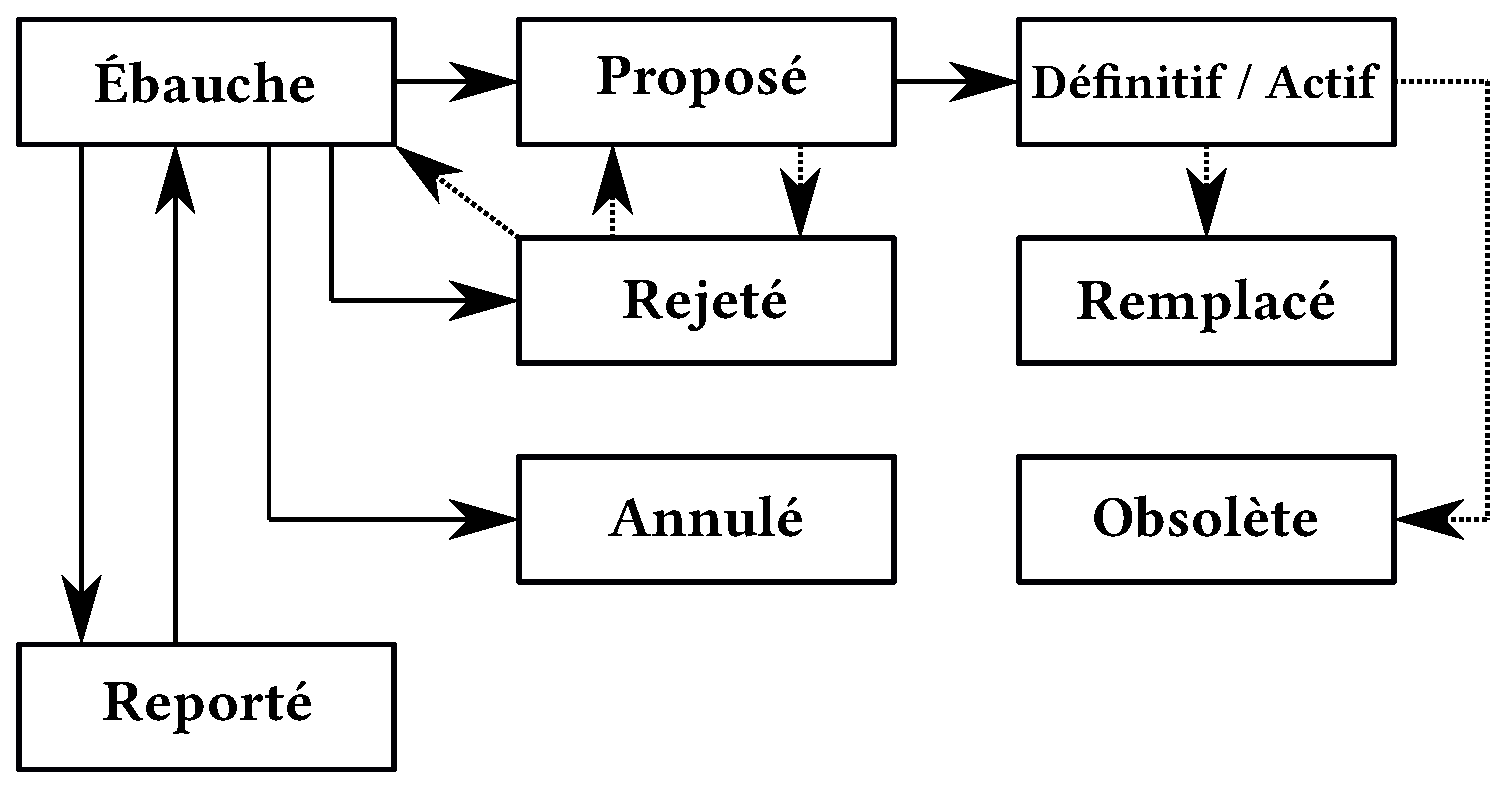
\includegraphics[scale=0.29]{img/bip-process-fr.eps}
  \caption{Schéma de la procédure d'adoption d'un BIP, inspiré du BIP-1.}
\end{figure}

% Utilisation des BIP pour les autres protocoles
Notez que ces documents sont utilisés pour BTC mais également pour d'autres protocoles. Par exemple, les BIP décrivant le fonctionnement des portefeuilles (BIP-32, BIP-39, BIP-44) sont valides pour la grande majorité des cryptomonnaies. Le SLIP-44 recense les cryptomonnaies compatibles avec le BIP-44\pagenote{«~SLIP-44~»~: \url{https://github.com/satoshilabs/slips/blob/master/slip-0044.md}}.

% Autres systèmes de propositions
Les autres protocoles cryptoéconomiques disposent même parfois de leurs propres systèmes de propositions. Ethereum utilise les EIP (\eng{Ethereum Improvement Proposals}), Bitcoin Cash les CHIP\pagenote{«~les CHIP~»~: \url{https://bch.info/en/chips}.} (\eng{Cash Improvement Proposals}), Litecoin les LIP\pagenote{«~les LIP~»~: \url{https://github.com/litecoin-project/lips}.}, etc.

\section*{La vérification des règles de consensus}
\addcontentsline{toc}{section}{La vérification des règles de consensus}

Bitcoin se base sur un réseau public d'ordinateurs accessible librement sur Internet. Ce réseau suit un modèle pair-à-pair, c'est-à-dire un modèle dans lequel tous les membres du réseau, appelés des nœuds, possèdent les mêmes privilèges. Ce sont ces nœuds qui s'assurent que les règles de consensus sont respectées. Si un bloc est invalide (en contenant une transaction invalide par exemple), alors il est rejeté par les nœuds appliquant les règles.

Dans Bitcoin, le rôle des nœuds est d'entretenir une copie du registre des transactions (la fameuse chaîne de blocs) et, ce faisant, de s'assurer de la validité des transactions et des blocs. Pour cela, ils communiquent avec les autres nœuds du réseau et relaient les nouvelles transactions et les nouveaux blocs, qui émanent respectivement des utilisateurs et des mineurs.

% Vérification complète
La vérification des règles de consensus peut être complète. Dans ce cas, on utilise parfois le pléonasme «~nœuds complets~» ou «~\eng{full node}~» pour insister sur le fait qu'ils vérifient l'intégralité de la chaîne. Ils téléchargent l'intégralité de la chaîne de blocs, vérifient les règles de consensus et relaient les blocs et les transactions. C'est une charge, que ce soit au niveau de la conservation des données (en novembre 2023, la chaîne de Bitcoin pesait environ 530~Go de données et l'ensemble des UTXO plus de 8,5~Go) que de la bande passante (la taille moyenne des blocs minés toutes les 10 minutes gravitait autour de 1,7~Mo en novembre 2023).

% Nœuds réduits
Les nœuds réduits (\eng{pruned nodes}), qui conservent l'état du réseau mais pas l'entièreté de la chaîne, sont des nœuds à part entière puisqu'ils ont vérifié la conformité des règles sur l'intégralité de la chaîne. Ils ne sont juste pas en mesure d'accéder à l'historique de la chaîne précédant une certaine date.

% Vérification partielle
La vérification peut aussi être partielle, auquel cas on parle de client léger (ou de «~nœud léger~» par abus de langage). Cela est utile pour les personnes qui n'ont pas l'intérêt de faire tourner un nœud complet. C'est par exemple le cas dans les logiciels de hachage (mettant en œuvre Stratum) et dans les portefeuilles légers. Ils utilisent en particulier une méthode conceptualisée dans le livre blanc de Bitcoin en 2008~: la vérification de paiement simplifiée\sendnote{Satoshi Nakamoto décrivait la vérification de paiement simplifiée comme suit~:
\begin{quote}
\footnotesize «~Il est possible de vérifier les paiements sans faire fonctionner un nœud complet du réseau. Un utilisateur a seulement besoin de conserver une copie des entêtes des blocs de la plus longue chaîne de preuves de travail, qu'il peut obtenir en interrogeant les nœuds du réseau jusqu'à ce qu'il soit convaincu qu'il possède la plus longue chaîne, et obtenir la branche de Merkle liant la transaction au bloc dans lequel elle est horodatée. Il ne peut pas vérifier la transaction par lui-même, mais en la reliant à un endroit de la chaîne, il peut voir qu'un nœud du réseau l'a acceptée, et les blocs ajoutés après le confirment.~»
\end{quote}
Satoshi Nakamoto, \emph{Bitcoin : un système d'argent liquide électronique pair-à-pair}, 31 octobre 2008.}.

% Vérification de paiement simplifiée
La vérification de paiement simplifiée (nommée en anglais \eng{Simplified Payment Verification} et abrégée en SPV) est une méthode astucieuse, qui permet aux utilisateurs néophytes et occasionnels de pouvoir interagir facilement avec le protocole sans devoir gérer un nœud complet, ni devoir faire aveuglément confiance à un dépositaire. Elle permet de réduire considérablement la charge des portefeuilles légers.  % contribue au succès de Bitcoin

% Chaîne d'entêtes
La vérification de paiement simplifiée se fonde sur la façon dont les blocs de transactions sont chaînés et structurés comme nous avons pu le voir dans le chapitre~\ref{ch:confirmation}. Premièrement, la chaîne de preuve de travail n'est pas à proprement parler une chaîne de blocs, mais une chaîne d'entêtes. Cela fait que les clients légers n'ont qu'à conserver cette chaîne des entêtes pour déterminer la chaîne possédant le plus de travail accumulé. Puisque chaque entête pèse 80 octets, la taille des données à conserver reste modeste pour des appareils modernes~: elle augmente d'environ 4~Mio par an, ce qui représentait un peu plus de 62 Mio en novembre 2023.

% Arbres de Merkle
Deuxièmement, les transactions sont agencées dans un arbre de Merkle, de sorte que les clients légers peuvent se contenter de demander les informations liées à la branche qui les intéressent pour s'assurer de la confirmation d'une de leurs transactions. Le nombre d'empreintes à obtenir et de hachages à effectuer dépend du logarithme binaire ($\log_{2}$) du nombre de transactions présentes dans le bloc. Pour un bloc de 3000 transactions (moyenne haute sur BTC), la charge correspond à demander 12 empreintes de 32 octets et à calculer 12 hachages pour procéder à la vérification.

% Défauts de fiabilité, de confidentialité et de vérification
Cette vérification simplifiée permet d'alléger la charge des portefeuilles, mais elle présente des défauts majeurs. D'abord, elle manque de fiabilité~: les nœuds ne peuvent pas mentir en inventant une transaction, mais peuvent omettre de transmettre des informations nécessaires. Ce défaut peut être partiellement contrebalancé en augmentant la diversité des connexions sur le réseau. Cependant, même dans ce cas, la vérification est vulnérable si la chaîne est attaquée par une entité disposant de la puissance de calcul majoritaire\sendnote{Ce cas a été décrit par Satoshi Nakamoto dans le livre blanc :
\begin{quote}
\footnotesize «~De ce fait, la vérification est fiable tant que les nœuds honnêtes contrôlent le réseau, mais est plus vulnérable si le réseau est maîtrisé par un attaquant. Alors que les nœuds du réseau peuvent vérifier les transactions par eux-mêmes, la méthode simplifiée peut être trompée par des transactions forgées par l'attaquant aussi longtemps que celui-ci maîtrise le réseau. Une stratégie pour se protéger serait d'accepter les alertes des nœuds du réseau lorsqu'ils détectent un bloc invalide, invitant le logiciel de l'utilisateur à télécharger le bloc complet et les transactions suspectes pour confirmer l'incohérence. Les entreprises qui reçoivent fréquemment des paiements voudront probablement toujours faire fonctionner leurs propres nœuds afin d'obtenir une sécurité plus indépendante et une vérification plus rapide.~»
\end{quote}
(Satoshi Nakamoto, \eng{Bitcoin: A Peer-to-Peer Electronic Cash System}, 31 octobre 2008.)

Les alertes décrites par Satoshi sont aujourd'hui appelées preuves de fraude mais sont toujours en phase de développement.}.

% Défaut de confidentialité
Ensuite, la vérification simplifiée possède aussi une insuffisance de confidentialité, car le client doit dévoiler une partie de son activité transactionnelle par les requêtes réalisées auprès des noeuds du réseau. Une façon de corriger partiellement ce problème est d'accroître le nombre d'informations demandées pour dissimuler les informations essentielles, mais cette méthode est plus qu'imparfaite\sendnote{Une première façon de remédier au problème de confidentialité était de mettre en place des filtres de Bloom, tels que décrits dans le BIP-37, mais cette méthode était peu efficace. Voir Arthur Gervais, Srdjan Capkun, Ghassan O. Karame, Damian Gruber, \eng{On the Privacy Provisions of Bloom Filters in Lightweight Bitcoin Clients}, décembre 2014~: \url{https://eprint.iacr.org/2014/763.pdf}. Il existe également Neutrino, décrit dans le BIP-157 et le BIP-158, qui fait usage du codage de Golomb-Rice et demande une plus grande bande passante.}.

% Défaut de vérification
Enfin, elle présente un défaut de vérification, en étant par définition partielle. Toutes les règles de consensus ne sont pas vérifiées, ce qui fait que les nœuds complets peuvent convenir d'un changement de règle qui ne sera pas remarqué par le client léger. Par exemple, les clients SPV ne vérifient pas les contraintes appliquées sur la taille des blocs, et le réseau pourrait donc subir une modification de cette limite sans qu'ils s'en rendent compte. C'est ce qui explique la stratégie des promoteurs de SegWit2X en 2017, qui prévoyaient de doubler la taille limite des blocs sans protection contre la rediffusion afin que les portefeuilles à vérification de paiement simplifiée suivent simplement la chaîne la plus longue\pagenote{«~prévoyaient de doubler la taille limite des blocs sans protection contre la rediffusion afin que les portefeuilles à vérification de paiement simplifiée suivent simplement la chaîne la plus longue~»~: Mike Belshe, \eng{[Bitcoin-segwit2x] Strong 2-Way Replay Protection}, \wtime{08/10/2017 20:16:02 UTC}~: \url{https://lists.linuxfoundation.org/pipermail/bitcoin-segwit2x/2017-October/000323.html}~ «~Aujourd'hui, nous sommes en bonne voie pour déployer segwit2x avec une grande majorité de mineurs qui le signalent encore. En plus de cela, 99,94~\% des nœuds et des clients SPV suivront automatiquement la chaîne la plus longue (segwit2x).~»}. % automatically follow that longest chain (segwit2x)

% Avis de Satoshi
Satoshi pensait que le système pourrait perdurer avec une vérification centralisée entre les mains de quelques nœuds vérificateurs (dont les mineurs) et que le reste des utilisateurs ferait usage des clients légers\pagenote{«~Satoshi pensait que le système pourrait perdurer avec une vérification centralisée entre les mains de quelques nœuds vérificateurs~»~: Satoshi Nakamoto a conservé cette vision jusqu'à son départ, comme en témoigne son courriel à Mike Hearn du 29 décembre 2010~:
\begin{quote}
\footnotesize «~Un jour, lorsque nous aurons des implémentations fonctionnant uniquement en mode client, la taille de la chaîne de blocs n'aura plus beaucoup d'importance. D'ici là, tant que tous les utilisateurs ont toujours à télécharger la chaîne de blocs entière pour commencer, il est bon de pouvoir la maintenir à une taille raisonnable.~»
\end{quote}
Satoshi Nakamoto, \eng{Re: More BitCoin questions}, \wtime{29/12/2010 21:42 UTC}~: \url{https://plan99.net/~mike/satoshi-emails/thread3.html}.}. Dans sa première réponse à James A. Donald en novembre 2008, il indiquait ainsi~: % "Eventually when we have client-only implementations, the block chain size won't matter much. Until then, while all users still have to download the entire block chain to start, it's nice if we can keep it down to a reasonable size."

\begin{quote}
«~Bien avant que le réseau n'atteigne cette taille, les utilisateurs pourront utiliser la vérification de paiement simplifiée (section 8) pour contrôler les doubles dépenses, ce qui ne nécessite que la chaîne des entêtes de bloc, soit environ 12~Ko par jour. Seules les personnes essayant de créer de nouvelles pièces auront besoin de faire fonctionner des nœuds de réseau.\sendnote{Satoshi Nakamoto, \eng{Re: Bitcoin P2P e-cash paper}, \wtime{03/11/2008, 01:37:43 UTC}~: \url{https://www.metzdowd.com/pipermail/cryptography/2008-November/014815.html}.}~»
\end{quote} % "Long before the network gets anywhere near as large as that, it would be safe for users to use Simplified Payment Verification (section 8) to check for double spending, which only requires having the chain of block headers, or about 12KB per day.  Only people trying to create new coins would need to run network nodes."

En cela, il se trompait. La vérification des règles de consensus a besoin d'être intégrale pour que celles-ci soient appliquées.

% Utilité systémique de cette vérification
C'est donc au niveau du nœud complet que se joue cette vérification, Cette réalité est parfois retranscrite par l'adage «~pas ton nœud, pas tes règles\sendnote{Understanding Bitcoin, \eng{Not Your Node Not Your Rules! w/ Ketominer, Udi Wertheimer, Francis Pouliot \& Mir Liponi}, 5 avril 2019~: \url{https://www.youtube.com/watch?v=jwaKVIEm-rI}.}\pagenote{«~pas ton nœud, pas tes règles~»~: L'adage «~\eng{not your node, not your rules}~» a été naturellement calqué sur l'adage «~\eng{not your keys, not your coins}~» (voir par exemple ce tweet de Udi Wertheimer~: \url{https://twitter.com/udiWertheimer/status/936215582487261184}). Il a été popularisé par le panel du même nom lors de la conférence Understanding Bitcoin, le 5 avril 2019. Le projet RaspiBlitz en a fait son slogan en 2020~: \url{https://github.com/rootzoll/raspiblitz/blob/bbeb5b21a982eeeb93306537e0aca2474bd23e03/README.md}.}~». Ne faites pas confiance, vérifiez~! Un peu comme une langue résulte des choix que font ses locuteurs, un protocole informatique résulte des règles appliquées par les nœuds complets. Cette vérification joue donc un rôle crucial dans la détermination du protocole.

\section*{Les hard forks}
\addcontentsline{toc}{section}{Les hard forks}

% Modification des règles de consensus
Puisque Bitcoin est ouvert et libre, les règles de consensus peuvent être modifiées à volonté par les nœuds du réseau au moyen d'un changement d'acceptation des blocs et des transactions. Ces modifications peuvent mener à des conflits sur le réseau, et éventuellement à la séparation en deux réseaux distincts gérant chacun sa propre chaîne et sa propre monnaie. D'où l'utilisation du mot \eng{fork}, qui signifie «~embranchement~», «~bifurcation~» ou «~fourche~» en français, pour parler de ce phénomène.

% Classification : hard forks et soft forks
Les modifications des règles de consensus sont couramment rangées en deux catégories~: celle des \eng{hard forks}, qui constituent des mises à niveau brutes et incompatibles, et celle des \eng{soft forks}, qui présentent une certaine rétrocompatibilité. Voyons comment ces changements se manifestent, en commençant par les hard forks, avant de décrire les soft forks.

% Polysémie du mot fork
Dans Bitcoin, il existe une polysémie au sujet du mot \eng{fork}, qui possède quatre significations différentes~: le fork logiciel, le fork de règles de consensus, le fork de chaîne commun et le fork de chaîne persistant. Cette polysémie prête à confusion de sorte qu'on préfère utiliser un terme différent pour chacun de ces sens.

% Fork logiciel
Comme on l'a dit, le mot fork est d'abord utilisé dans le développement logiciel, notamment dans le cadre du logiciel libre qui autorise et encourage ce type de pratique. Il désigne la création d'un programme dérivé du code source d'un programme existant et aussi, par abus de langage, le programme dérivé en lui-même. En ce sens, l'implémentation de référence peut subir un embranchement, créant un logiciel alternatif. Ce logiciel peut respecter les règles de consensus (comme par exemple Bitcoin Knots), mais il peut aussi les faire dévier, en créant un nouveau protocole qui partage l'historique de la chaîne (Bitcoin ABC, devenu Bitcoin Cash Node) ou non (Litecoin).

% Embranchement commun de la chaîne
Le fork peut ensuite désigner l'embranchement commun de la chaîne de blocs, par analogie avec le développement logiciel. La chaîne de blocs n'est en effet pas une structure linéaire, mais une «~structure en forme d'arbre\sendnote{Satoshi Nakamoto, code source de la version 0.1 du logiciel Bitcoin~: \url{https://github.com/trottier/original-bitcoin/blob/4184ab26345d19e87045ce7d9291e60e7d36e096/src/main.h\#L1001-L1008}.}~» qui peut posséder de multiples branches de blocs, pareillement compatibles avec les règles de consensus acceptées par le réseau, la sélection de la branche correcte se faisant par la plus longue (possédant le plus de travail accumulé). Ce type d'embranchement se produit régulièrement dans Bitcoin de manière tout à fait normale et bénigne, lorsque deux mineurs trouvent simultanément un bloc différent de leur côté, et est résolu lorsqu'un nouveau bloc est trouvé.

% Scission
Le fork peut aussi se rapporter à une scission de la chaîne de blocs causée par une incompatibilité des règles de consensus. On parle alors de hard fork, c'est-à-dire littéralement d'«~embranchement dur~». Cette scission est généralement permanente dans le sens où les deux branches ne peuvent pas se réconcilier par le mécanisme de consensus de Nakamoto, sauf dans un cas très précis~: si les règles de la branche majoritaire forment une sous-partie restrictive des règles de la branche minoritaire. Les deux chaînes résultantes sont, à terme, vouées à exister sur des réseaux séparés.

% Conflit des règles de consensus
Enfin, le terme fork peut, par métonymie, désigner une modification des règles de consensus, qui est toujours susceptible de provoquer une scission de chaîne et une séparation du réseau. Une restriction des règles de consensus est appelée un soft fork, littéralement «~embranchement doux~», en vertu de sa capacité à résulter en une branche unique. Toute autre modification des règles de consensus, qu'il s'agisse d'une extension ou d'une modification strictement incompatible, est appelée un hard fork, en référence à sa propension à créer une scission de chaîne. C'est de ces deux modifications dont nous voulons parler ici.\sendnote{Notez que les concepts sont liés. Ainsi, un fork logiciel (copie et modification) peut implémenter un fork des règles de consensus (hard fork ou soft fork) qui finira par créer un fork persistant de la chaîne (scission).}

% Hard fork
Le hard fork est le concept le plus ancien si on le compare au soft fork. Il était auparavant qualifié de «~changement incompatible\sendnote{David François (davout), \eng{Re: Small protocol changes for flexibility}, \wtime{07/12/2010 15:08:02 UTC}~: \url{https://bitcointalk.org/index.php?topic=894.msg27757\#msg27757}.}~». Le hard fork est une modification non restrictive des règles de consensus. Il provoque un conflit sur le réseau entre les nœuds qui appliquent les anciennes règles et les nœuds qui appliquent les nouvelles.

% Hard fork extensif
Un hard fork peut être extensif, c'est-à-dire élargir les règles de consensus sur les blocs et les transactions. Les anciens peuvent ainsi produire des blocs valides sur la nouvelle chaîne, mais pas l'inverse. L'exemple typique de ce genre de hard fork est l'augmentation de la taille limite des blocs, qui consiste à accepter des blocs ayant une taille ou un poids plus grand, comme 2~Mo au lieu de 1~Mo ou 8~MWU à la place de 4~MWU. Ce hard fork extensif est illustré sur la figure~\ref{fig:expanding-hard-fork}.

\begin{figure}[h]
  \centering
  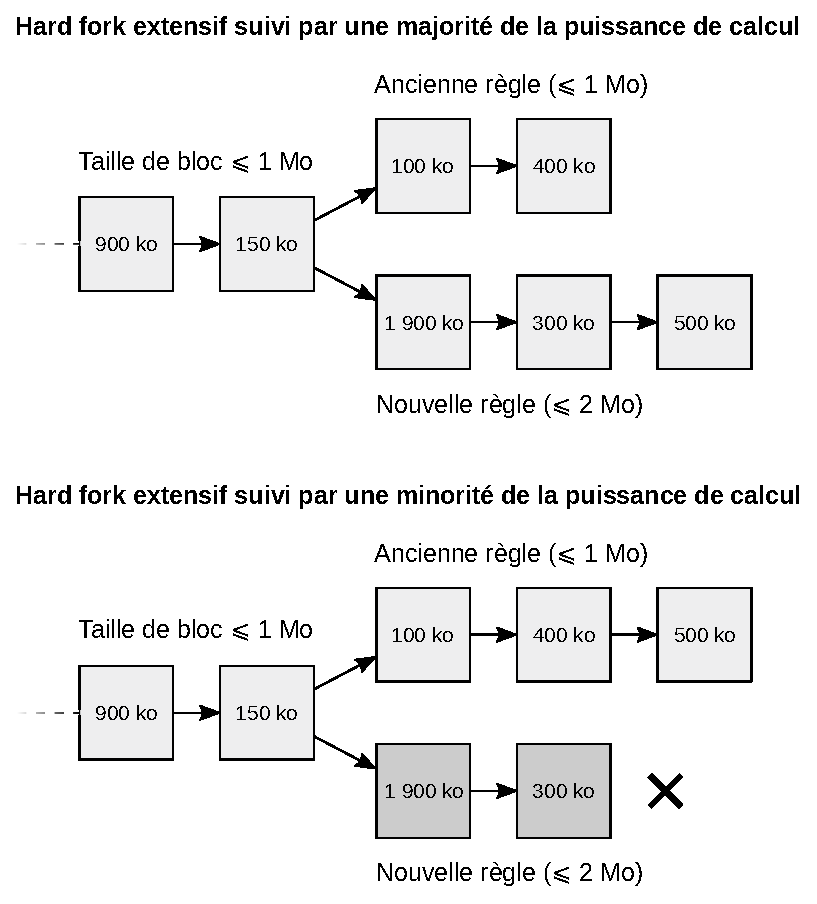
\includegraphics[scale=0.65]{img/expanding-hard-fork-induced-forks.eps}
  \caption{Schéma d'un hard fork extensif~: si la chaîne suivant la nouvelle règle est plus longue que celle suivant l'ancienne, les deux chaînes persistent~; dans le cas contraire, seule la deuxième survit.}
  \label{fig:expanding-hard-fork}
\end{figure}

% Destruction par recoordination
Dans le cas où le hard fork extensif n'est pas soutenu par une majorité de la puissance de calcul du réseau, celui-ci risque de ne pas créer une branche persistante. Par exemple, les blocs de la branche imposant une limite de taille plus petite sont entièrement compatibles avec les nouvelles règles, de sorte que, si elle est plus longue, c'est elle qui sera sélectionnée comme la branche correcte. C'est pour éviter cette situation problématique que les hard forks sont généralement bilatéraux.

% Hard fork bilatéral
Le hard fork bitatéral est un hard fork qui crée une incompatibilité totale entre les nouvelles règles et les anciennes. Il peut s'agir d'une règle ajoutée comme l'exigence que le premier bloc de l'embranchement inclue un changement incompatible. Dans notre cas de l'augmentation de la taille limite des blocs, il s'agirait d'imposer au premier bloc d'être strictement plus gros que la taille limite précédente, comme on le voit sur la figure~\ref{fig:expanding-hard-fork-failure}. Cette règle supplémentaire est appelée protection contre la destruction par recoordination (ou \eng{wipeout protection} en anglais).

\begin{figure}[h]
  \centering
  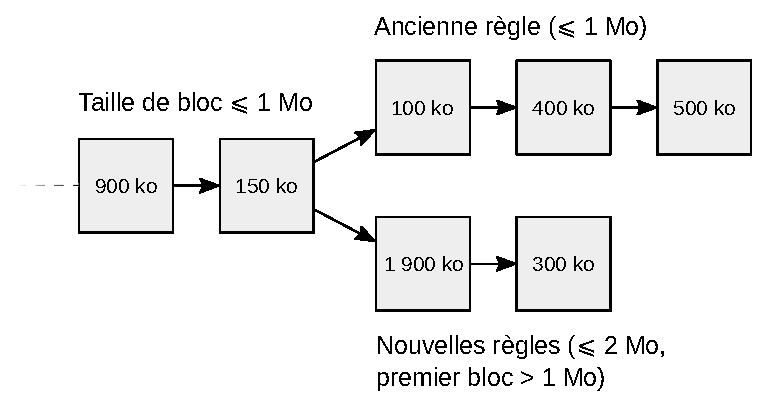
\includegraphics[scale=0.65]{img/bilateral-hard-fork-induced-fork.eps}
  \caption{Schéma d'un hard fork bilatéral~: les nouvelles règles sont strictement incompatibles avec les anciennes règles, de sorte que les deux chaînes persistent.}
  \label{fig:expanding-hard-fork-failure}
\end{figure}

% Autre exemple de hard fork bilatéral
Un autre exemple est le changement de l'algorithme de signature des transactions, qui rend l'intégralité des transactions signées et des blocs non vides strictement incompatibles. Ce changement a pour effet de permettre en plus une protection contre la rediffusion des transactions (\eng{replay protection}), dans le cas où deux chaînes concurrentes persisteraient.

% Deux hard forks, deux intentions
Deux situations peuvent découler d'un hard fork~: soit la quasi-totalité de l'économie procède au changement, auquel cas une seule chaîne subsiste~; soit l'économie se fragmente, auquel cas les deux chaînes persistent. La première situation est visée par le hard fork de mise à niveau qui n'a pas vocation à créer deux chaînes distinctes. La seconde est désirée par le hard fork contentieux, résultant d'une division de la communauté au sujet du changement. Le hard fork accidentel, créé par une modification non désirée des règles de consensus implicites, est écarté ici\sendnote{Le 11 mars 2013, le passage de la version 0.7 du logiciel à la version 0.8 implémentait la migration du système de base de données de Berkeley DB à LevelDB. Toutefois, il s'avérait que Berkeley DB faisait intervenir une limite par défaut (\eng{lock limit}) qui n'était pas présente dans LevelDB. Par conséquent, la migration constituait un hard fork accidentel et a provoqué un embranchement à partir du bloc 225~430 qui a duré environ 6 heures. La décision a finalement été prise de revenir à la version 0.7, invalidant la branche de 24 blocs minée du côté de la version 0.8, et de procéder à la migration quelques mois plus tard. -- Voir Vitalik Buterin, \eng{Bitcoin Network Shaken by Blockchain Fork}, 13 mars 2013~: \url{https://bitcoinmagazine.com/technical/bitcoin-network-shaken-by-blockchain-fork-1363144448}~; Gavin Andresen, \eng{BIP-50: March 2013 Chain Fork Post-Mortem}, ~: \url{https://github.com/bitcoin/bips/blob/master/bip-0050.mediawiki}. Une double dépense conséquente a été réalisée~: macbook-air, \eng{A successful DOUBLE SPEND US\$10000 against OKPAY this morning.}, \wtime{12/03/2013, 18:22:02 UTC}~: \url{https://bitcointalk.org/index.php?topic=152348.msg1616747\#msg1616747}.}.

% Hard fork de mise à niveau
Le hard fork de mise à niveau est un hard fork qui nécessite une synchronisation de la quasi-totalité de la communauté. Il résulte généralement en une seule chaîne, de sorte qu'on peut considérer que le protocole a été mis à niveau, alors qu'il s'agit essentiellement d'une utilisation économique qui passe d'un protocole à un autre. Il peut pour cela être extensif, même si la bilatéralité est préférée pour des raisons de sécurité.

% Exemples de hard forks de mise à niveau sur BTC
Le premier hard fork de mise à niveau connu est probablement l'ajout des codes opération \texttt{OP\_NOP} à la version 0.3.6 de Bitcoin par Satoshi Nakamoto en juillet 2010. L'augmentation de la taille des blocs était également pensée comme un hard fork de mise à niveau, notamment par Satoshi lui-même\sendnote{En octobre 2010, à la suite de la proposition de Jeff Garzik d'augmenter la limite directement à 7,168~Mo afin d'«~égaler le taux transactionnel moyen de PayPal~», Satoshi -- bien conscient qu'il s'agissait d'un correctif «~incompatible avec le réseau~» -- écrivait~:
\begin{quote}
\footnotesize «~[La mise à niveau] peut être introduite progressivement, par exemple~:

if (blocknumber > 115000)
  maxblocksize = largerlimit

Elle peut commencer à être intégrée dans les versions bien avant, de sorte qu'au moment où elle atteint le numéro de bloc et entre en vigueur, les anciennes versions qui ne l'ont pas sont déjà obsolètes.

Lorsque nous approchons du numéro de bloc limite, je peux envoyer une alerte aux anciennes versions pour qu'elles sachent qu'elles doivent effectuer une mise à jour.~»
\end{quote}
Satoshi Nakamoto, \eng{Re: [PATCH] increase block size limit}, \wtime{04/10/2010 19:48:40 UTC}~: \url{https://bitcointalk.org/index.php?topic=1347.msg15366\#msg15366}.}, jusqu'au hard fork contentieux de Bitcoin Cash en 2017.

% Exemples de hard forks de mise à niveau hors BTC
En dehors de BTC, les mises à niveaux par hard fork sont nombreuses, notamment en raison d'une économie moins grande et~/~ou plus centralisée. On peut citer les cas de Bitcoin Cash, de Monero, d'Ethereum Classic et d'Ethereum, où des mises à niveau de ce type sont réalisées régulièrement.

% Hard fork contentieux
Le hard fork contentieux est un hard fork visant délibérément à créer une nouvelle chaîne. Il est issu d'une dissension dans la communauté, qui est si forte qu'elle pousse à la sécession. Il est généralement bilatéral.

% Exemple de hard fork contentieux : ETC / ETH
Le premier exemple de hard fork contentieux majeur est celui qui a eu lieu sur Ethereum en juillet 2016, dans le contexte du piratage de TheDAO\pagenote{«~celui qui a eu lieu sur Ethereum en juillet 2016~»~: Simon Polrot, \emph{The DAO~: post mortem}, 24 janvier 2017~: \url{https://www.ethereum-france.com/the-dao-post-mortem/}~; Casey Detrio, \eng{EIP-779: Hardfork Meta: DAO Fork}, 26 novembre 2017~: \url{https://eips.ethereum.org/EIPS/eip-779}.}. Ce hard fork consistait à reprendre les fonds du pirate par un «~changement d'état irrégulier~». Celui-ci était rendu bilatéral par la règle imposant aux 10 premiers blocs d'inclure la chaîne de caractères \longstring{dao-hard-fork}. Puisque la majorité économique se trouvait du côté de l'annulation, la chaîne altérée a gardé le nom d'Ethereum et le sigle boursier ETH, tandis que l'autre chaîne a pris le nom d'Ethereum Classic et le sigle boursier ETC.

% Exemple de hard fork contentieux : BTC / BCH
Le second exemple de hard fork contentieux est celui qui a mené à la création de Bitcoin Cash en août 2017 suite au débat sur la scalabilité et à la guerre des blocs\pagenote{«~celui qui a mené à la création de Bitcoin Cash en août 2017~»~: Ludovic Lars, \emph{Bitcoin Cash~: la branche minoritaire issue du débat sur la scalabilité}, 30 janvier 2022~: \url{https://journalducoin.com/analyses/bitcoin-cash-branche-minoritaire-debat-scalabilite/}~; \eng{BCH-UAHF: Bitcoin Cash User-Activated Hard Fork}, 24 juillet 2017~: \url{https://reference.cash/protocol/forks/bch-uahf}.}. Ce hard fork n'intégrait pas SegWit, augmentait la taille limite des blocs à 8~Mo et améliorait l'algorithme de signature. Il était rendu bilatéral par une règle qui imposait au bloc suivant l'activation d'avoir une taille strictement supérieure à 1~Mo. Il offrait aussi \emph{de facto} une protection contre la rediffusion des transactions. Ce changement ayant dû se faire sans l'accord de la majorité économique, la chaîne qui ne modifiait pas les règles a pu conserver le nom de Bitcoin et le sigle boursier BTC, tandis que la nouvelle chaîne a dû adopter un nouveau nom, Bitcoin Cash, et un nouveau sigle, BCH.

\begin{figure}[h]
  \centering
  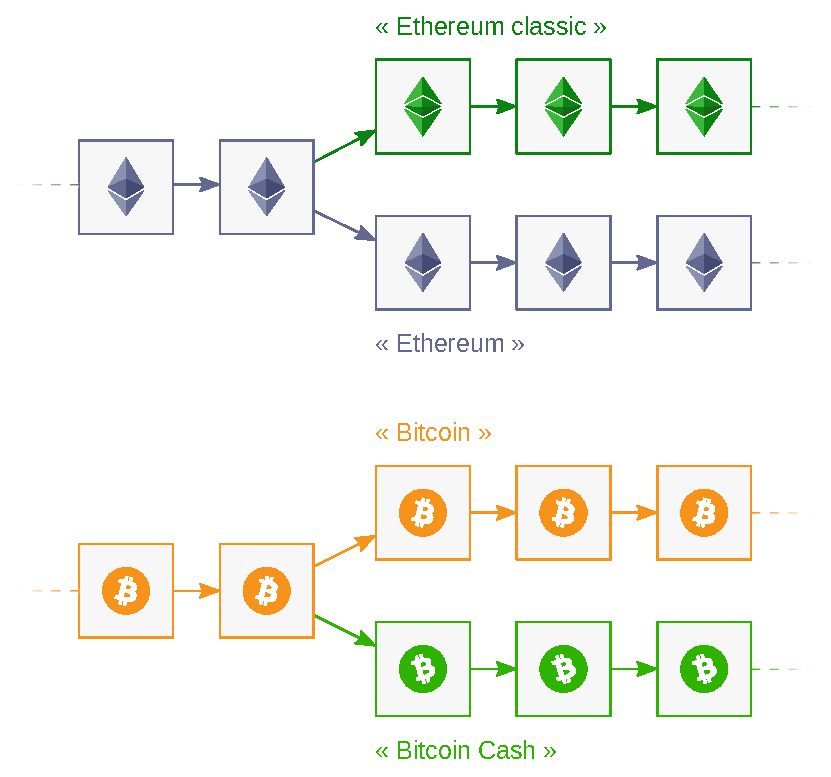
\includegraphics[scale=0.65]{img/hard-forks-eth-etc-bch-btc.eps}
  \caption{Exemples de hard forks bilatéraux~: ETH~/~ETC et BCH~/~BTC.}
  \label{fig:hard-forks-eth-bch}
\end{figure}

% Ajustement de la difficulté
Notez qu'un tel hard fork peut être amené à modifier l'algorithme d'ajustement de la difficulté. En effet, si la puissance de calcul est trop faible pour le soutenir, il est possible que l'ajustement n'arrive pas à terme. C'est pour cette raison que Bitcoin Cash a dû implémenter un \eng{Emergency Difficulty Adjustment} (EDA) qui a permis de procéder à l'adaptation sur une période plus courte. Ethereum Classic n'a cependant pas dû le faire, car l'ajustement sur Ethereum avait déjà lieu à tous les blocs.

\section*{Les soft forks}
\addcontentsline{toc}{section}{Les soft forks}

% Définition
Passons maintenant au soft fork, qui est un procédé de mise à niveau souvent mal compris. Le soft fork est une restriction des règles de consensus. Il consiste ainsi par essence à rendre l'ensemble des blocs et des transactions valides plus petit, en ajoutant une règle ou en modifiant une règle existante de façon plus restrictive. L'exemple typique de ce genre de fork est la diminution de la taille limite des blocs. L'ajout de la limite explicite des 1~Mo en octobre 2010 était de ce fait un soft fork.

% Application par la puissance de calcul
Le soft fork peut être appliqué en conservant une seule et même chaîne. S'il est imposé par la majorité de la puissance de calcul du réseau, il n'y a aucun risque de scission. En effet, l'ensemble des blocs créés par les mineurs qui appliquent les nouvelles règles est entièrement compatible avec les anciennes règles, de sorte que la branche appliquant les nouvelles règles sera considérée comme la branche correcte par tous les nœuds si elle est majoritaire. Si l'application du soft fork est en revanche minoritaire, alors ce dernier résulte en deux chaînes persistantes distinctes. Les deux cas de figure sont illustrés sur la figure~\ref{fig:soft-fork}.

\begin{figure}[h]
  \centering
  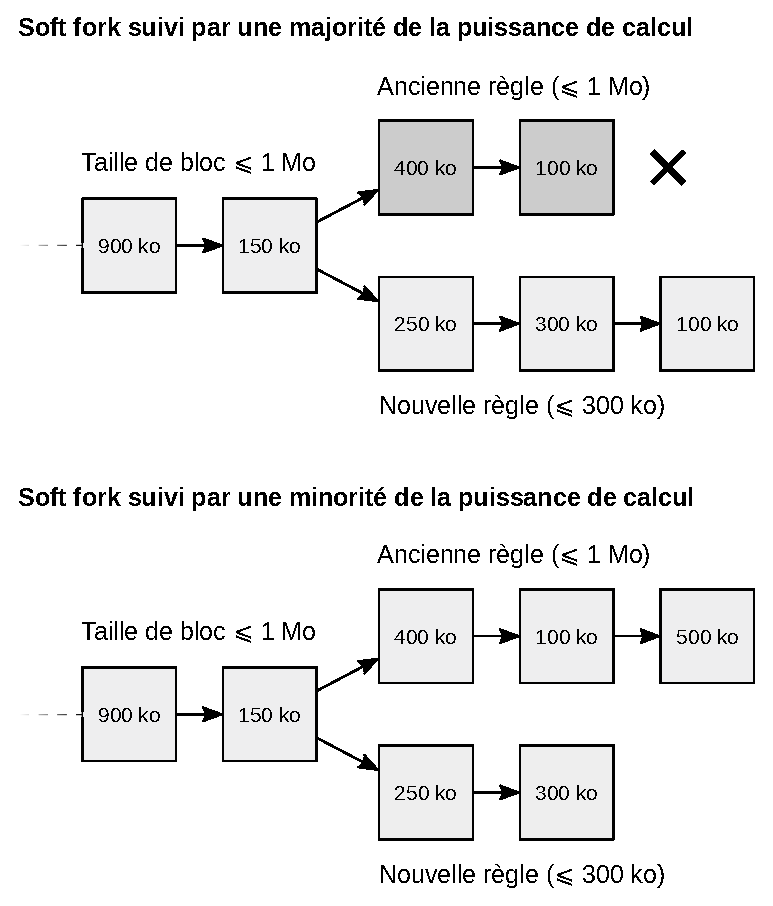
\includegraphics[scale=0.65]{img/soft-fork-induced-forks.eps}
  \caption{Schéma d'un soft fork~: si la chaîne suivant la nouvelle règle est plus longue que celle suivant l'ancienne, seule la première survit~; dans le cas contraire, les deux chaînes persistent.}
  \label{fig:soft-fork}
\end{figure}

% Origine
Le concept de soft fork est postérieur à celui de hard fork. Il a été formellement découvert par Gavin Andresen en octobre 2011 qui, suite à son étude de la proposition d'ajout du code opération \texttt{OP\_EVAL} par Nicolas van Saberhagen\sendnote{Nicolas van Saberhagen (ByteCoin), \eng{OP\_EVAL proposal}, \wtime{02/10/2011 00:49:19 UTC}~: \url{https://bitcointalk.org/index.php?topic=46538.msg553689\#msg553689}.}, s'est aperçu que la mise à niveau pouvait se faire grâce au code opération \texttt{OP\_NOP1} sans nécessairement provoquer de scission\sendnote{«~Je lis probablement mal le code, mais je pense que OP\_EVAL ne provoquerait pas de scission de blockchain~!~» s'est exprimé Gavin Andresen sur IRC. -- \#bitcoin-dev IRC logs, 2 octobre 2010~: \url{https://web.archive.org/web/20131201200245/http://bitcoinstats.com/irc/bitcoin-dev/logs/2011/10/02}.}.

% Codes opération
Les codes opération \texttt{OP\_NOP} sont des instructions du langage de script de Bitcoin qui ont été ajoutés dans le code par Satoshi en juillet 2010 avec pour seul commentaire «~expansion\sendnote{Satoshi Nakamoto, \eng{reverted makefile.unix wx-config -- version 0.3.6 (git commit)}, \wtime{29/07/2010 18:27:12 UTC}~: \url{https://sourceforge.net/p/bitcoin/code/119/}.}~». Le changement a été rendu effectif avec la version 0.3.6 du logiciel qui corrigeait également le 1 RETURN bug, publiée le 29 juillet\pagenote{«~la version 0.3.6 du logiciel [...] publiée le 29 juillet~»~: Satoshi Nakamoto, \eng{*** ALERT *** Upgrade to 0.3.6}, \wtime{29/07/2010 19:13:06 UTC}~: \url{https://bitcointalk.org/index.php?topic=626.msg6451\#msg6451}.}. Leur rôle est initialement muet~: s'ils sont présents dans un script, ils ne font rien mais ils n'invalident pas la transaction non plus. La conséquence directe est qu'on peut modifier le comportement de ces codes opération sans rendre les scripts incompatibles avec les anciennes règles de consensus. L'ajout de cette caractéristique indique donc que Satoshi avait saisi le mécanisme du soft fork.

% Échange sur IRC
% 16:40	gavinandresen	I'm probably reading the code wrong, but I think OP_EVAL wouldn't cause a blockchain split!
% 18:59	gmaxwell	wow. Gavin's point that EVAL can be done without a split blew my mind.
% 21:23	gmaxwell	You can also make the new code keep the old behavior for blocks before a certian height.
% 21:24	gmaxwell	So you can set the actual switch point at some point in the future.
% 21:25	gmaxwell	(so that you have time to actually achieve >>50% hashpower behind the change)
% 21:27	gmaxwell	e.g. make and backport a patch which will agressively not forwardward txn with the reserved NOP until block X, and after X start applying the new validation rules but only to future blocks. Then so long has >>50% hashpower is running this patch by block X there is no lasting fork created.

% Caractère postcompatible
Le soft fork possède un caractère «~rétrocompatible~» -- ou postcompatible à proprement parler, car la compatibilité est ascendante et non descendante -- dans le sens où les anciennes versions du logiciel peuvent continuer d'interagir avec le système. En effet, les nœuds non miniers suivant les anciennes règles continuent de voir les blocs produits comme valides. Cette caractéristique est un avantage majeur par rapport au hard fork.

% La rétrocompatibilité, ou compatibilité descendante, est la compatibilité d'un produit vis-à-vis de ses anciennes ou précédentes versions ; la compatibilité ascendante ou postcompatibilité est la compatibilité d'un produit vis-à-vis des versions plus récentes, voire encore en phase de conception.

% Inconvénients
Mais cette compatibilité ascendante ne veut pas dire qu'un soft fork est «~doux~». Il possède un côté pernicieux dans le sens où il rend la modification difficile à appréhender. Le soft fork présente ainsi plusieurs inconvénients.

% Non-optionnalité
D'abord, il n'est pas optionnel. S'il est appliqué par la majorité de la puissance de calcul, un soft fork s'apparente en effet à une attaque de censure pour les utilisateurs qui suivent les anciennes règles. Le soft fork possède donc un caractère coercitif que le hard fork n'a pas.

% Irréversibilité
Puis, le soft fork est difficilement réversible. Les fonctionnalités ajoutées ne peuvent pas être désactivées simplement~: une fois adopté, il n'y a pas de retour en arrière facile. Les développeurs de Bitcoin SV ont ainsi désactivé P2SH en février 2020 exposant les utilisateurs les moins attentifs à des vols\pagenote{«~Les développeurs de Bitcoin SV ont ainsi désactivé P2SH en février 2020~»~: Jon Southurst, \eng{Final Genesis specs released—bye P2SH}, 10 janvier 2020~: \url{https://coingeek.com/final-genesis-specs-released-bye-p2sh/}.}.

% Non-limitation
Ensuite, le soft fork n'est pas limité quant à ce qu'il peut faire. Il peut augmenter la limite effective de taille des blocs (via un bloc auxiliaire\pagenote{«~bloc auxiliaire~»~: \url{https://bitcointalk.org/index.php?topic=283746.msg3036293\#msg3036293}.} aussi appelé bloc d'extension\pagenote{«~bloc d'extension~»~: \url{https://lists.linuxfoundation.org/pipermail/bitcoin-dev/2015-May/008356.html}.} ou soft fork généralisé\pagenote{«~soft fork généralisé~»~: ZoomT, \eng{Increasing the blocksize as a (generalized) softfork.}, \wtime{20/12/2015 11:12:48 UTC}~: \url{https://bitcointalk.org/index.php?topic=1296628.msg13305141\#msg13305141}.}). Ce bloc d'extension peut également inclure des fonctionnalités supplémentaires (comme MimbleWimble dans Litecoin). Il peut même modifier la politique monétaire du protocole en redéfinissant l'unité de base\sendnote{La façon dont un soft fork peut introduire de l'inflation dans Bitcoin a été exposée par le développeur Peter Todd en 2016. -- Peter Todd, \eng{Forced Soft Forks}, 18 janvier 2016~: \url{https://petertodd.org/2016/forced-soft-forks}.}.

% Complexité
Enfin, le soft fork, s'il est profond, crée une complexité supplémentaire, liée aux contraintes de son application. En effet, il ajoute de nouvelles exceptions aux règles de consensus, ce qui génère de la dette technique pour les développeurs\pagenote{«~dette technique~»~: Ward Cunningham, «~The WyCash Portfolio Management System~», \eng{Addendum to the Proceedings of OOPSLA 1992}, octobre 1992~: \url{https://dl.acm.org/doi/pdf/10.1145/157710.157715}.}.

% (L'abominable) SegWit
L'archétype du soft fork profond et complexe a été la mise à niveau SegWit, ou \eng{Segregated Witness}, qui consistait à déplacer les données de signature des transactions (appelées témoin ou \eng{witness}) vers une structure de données séparée (\eng{segregated}) afin de supprimer la malléabilité des transactions. Cette mise à niveau, qui a eu lieu en le 24 août 2017, devait être initialement un hard fork, avant que le développeur luke-jr ne décrive en 2015 comment en faire un soft fork\pagenote{«~avant que le développeur luke-jr ne décrive en 2015 comment en faire un soft fork~»~: Aaron van Wirdum, \eng{The Long Road to SegWit: How Bitcoin's Biggest Protocol Upgrade Became Reality}, 23 août 2017~: \url{https://bitcoinmagazine.com/technical/the-long-road-to-segwit-how-bitcoins-biggest-protocol-upgrade-became-reality}.}. La rétrocompatibilité était assurée par la liaison du témoin au bloc via un arbre de Merkle dont la racine était placée dans la transaction de récompense et par l'utilisation de sorties transactionnelles dépensables par n'importe qui (\eng{anyone-can-spend}). Outre la correction du problème de malléabilité, elle a instauré un système de versionnage (qui a permis l'intégration de Schnorr-Taproot par la suite) et a modérément augmenté la capacité transactionnelle du réseau, de sorte que la taille effective des blocs pouvait dépasser 1~Mo, jusqu'à 4~Mo en théorie. Elle a également ajouté quatre nouveaux types d'adresse au protocole.

% Méthodes d'activation
De plus, le soft fork requiert la majorité de la puissance de calcul du réseau pour préserver son intérêt. S'il n'est pas suivi à moyen terme par 51~\% de la puissance de calcul, alors son application provoque une scission. C'est ce qui explique pourquoi l'activation par les mineurs est généralement préférée à l'activation par les utilisateurs, même si le pouvoir de décision revient à ces derniers comme on le verra dans le chapitre~\ref{ch:determination}.

% Soft fork activé par les utilisateurs
D'une part, le soft fork activé par les utilisateurs (en anglais \eng{user activated soft fork} ou UASF) consiste à implémenter le soft fork dans le code source du logiciel de sorte à ce qu'il rentre en application à une hauteur de bloc ou à un horodatage donné. Cette méthode s'appuie sur la confiance que l'économie appliquant la mise à niveau sera largement majoritaire et que l'activité minière suivra à moyen terme en raison d'une récompense de bloc plus élevée.

% Soft fork activé par les mineurs
D'autre part, le soft fork activé par les mineurs (en anglais \eng{miner activated soft fork} ou MASF) consiste à faire dépendre l'activation du signalement des mineurs au sein des blocs validés. Il est activé lorsqu'un certain seuil de signalement (95~\% par exemple) est dépassé. Cette méthode, dont la procédure a été notamment décrite dans le BIP-9, permet de s'assurer autant que possible que les mineurs appliquent la mise à niveau et qu'il ne subsiste qu'une seule chaîne.

% UAHF / MAHF
La même distinction existe dans l'activation des hard forks, mais celle-ci a peu de pertinence, la puissance de calcul ne pouvant pas empêcher la scission. Ainsi, le hard fork activé par les mineurs ou MAHF, longtemps soutenu par les partisans de l'augmentation de la taille limite des blocs, n'a pas d'intérêt particulier.

% Deux types de soft forks
Comme les hard forks, les soft forks peuvent être rangés en deux catégories plus ou moins distinctes~: le soft fork de mise à niveau et le soft fork contentieux.

% Soft fork de mise à niveau
Le soft fork est idéal pour mettre à niveau le protocole. Cela permet aux nœuds de ne pas se mettre à niveau tout de suite. Même s'il demande une certaine synchronisation, celle-ci n'est pas aussi contraignante que pour les hard forks.

% Exemples de soft forks de mise à niveau dans BTC
Dans BTC, le soft fork est ainsi privilégié par les développeurs depuis sa découverte. De nombreuses mises à niveau en étaient, comme \eng{Pay to Script Hash} (BIP-16), ou l'obligation de spécifier la hauteur du bloc dans la transaction de récompense (BIP-34), ou encore l'ajout d'un standard d'encodage des signatures (BIP-66). Les ajouts des codes opération \longstring{OP\_CHECKLOCKTIMEVERIFY} et \longstring{OP\_CHECKSEQUENCEVERIFY} permettant l'usage de verrous temporels dans le langage de script par l'utilisation respective des codes \texttt{OP\_NOP2} et \texttt{OP\_NOP3} ont également été des soft forks. Enfin, plus récemment, l'adoption de Schnorr-Taproot (ou Taproot pour faire court) a été une mise à niveau par soft fork.

% Exemples de soft forks de mise à niveau dans LTC
Litecoin fait aussi usage de ce type de transition. Le protocole a notamment intégré SegWit en mai 2017, ainsi que Schnorr-Taproot et MimbleWimble (MWEB) en mai 2022.

% Soft fork contentieux
Le soft fork contentieux a pour objectif de contraindre la minorité de la communauté à suivre la majorité. S'il réussit, il n'y a qu'une seule chaîne, les opposants ayant le choix d'accepter les règles ou de procéder eux-mêmes à un hard fork. S'il échoue, il en résulte en deux chaînes concurrentes.

% SegWit
SegWit est l'exemple typique d'un soft fork contentieux réussi. Il n'était pas approuvé par l'ensemble des acteurs importants (les partisans des gros blocs d'une part, les puristes du protocole comme Mircea Popescu d'autre part\sendnote{Mircea Popescu, \eng{There's a one Bitcoin reward for the death of Pieter Wuille. Details below.}, 10 décembre 2015~: \url{http://trilema.com/2015/theres-a-one-bitcoin-reward-for-the-death-of-pieter-wuille-details-below/}.}, s'y opposaient), mais il a recueilli un soutien majoritaire de sorte qu'il a pu perdurer et que les \eng{big blockers} mécontents ont dû migrer vers Bitcoin Cash.

% "Coinbase rule"
Un exemple de soft fork contentieux ayant échoué est la tentative de l'équipe de Bitcoin ABC d'imposer une redirection de 8~\% de la subvention de minage de Bitcoin Cash à son propre profit le 15 novembre 2020\sendnote{Amaury Séchet, \eng{Bitcoin ABC's plan for the November 2020 upgrade}, 6 août 2020~: \url{https://amaurysechet.medium.com/bitcoin-abcs-plan-for-the-november-2020-upgrade-65fb84c4348f}.}. Cette tentative, qui était un soft fork en raison de son caractère restrictif, a provoqué la scission entre une branche majoritaire sans redirection (BCH) et une branche minoritaire avec, qui a été par la suite renommée en «~eCash~» (XEC).

% Supériorité du soft fork
Ainsi, le soft fork, qu'il soit approuvé à l'unanimité ou bien seulement par une majorité, est une méthode supérieure au hard fork. Bien qu'il soit parfois plus complexe, il permet de ne pas requérir une synchronisation de l'économie entière, cette dernière pouvant s'y adapter progressivement, ce qui est un bienfait non négligeable dans le cas d'un système ouvert utilisé par une grande diversité de personnes comme Bitcoin. Le signalement supermajoritaire des mineurs permet de minimiser le risque de scission et de conserver l'effet de réseau au maximum.

% % Meilleure méthode de mise à niveau
% Les soft forks ont ainsi des caractéristiques précises qui font qu'ils possèdent des avantages, mais aussi des inconvénients, par rapport aux hard forks. Si la mise à niveau est profonde, le hard fork a l'avantage d'être simple, tandis que le soft fork peut présenter une certaine complexité. Le hard fork requiert que l'ensemble du réseau se synchronise pour appliquer la mise à niveau, tandis que le soft fork ne demande qu'une synchronisation de la puissance de calcul majoritaire et une adaptation progressive de l'économie. De ce fait, la probabilité d'une scission est plus élevée dans le cas d'un hard fork que dans celui d'un soft fork qui aurait fait l'objet d'un signalement supermajoritaire des mineurs, ce qui permet la conservation de l'effet de réseau.

% Sacrifice du consentement
Mais cet avantage majeur se fait au prix d'un sacrifice~: celui de la clarté du consentement. Dans le cas du hard fork, le consentement est clair~: les personnes qui souhaitent la modification se retrouvent sur la chaîne qu'elles ont choisie. Dans le cas du soft fork, le consentement est plus ambigu~: le fait d'opérer sur la chaîne n'indique pas nécessairement une acceptation active du changement, mais une résignation passive et un refus de réaliser un hard fork minoritaire. Comme l'écrivait brillamment Vitalik Buterin en mars 2017~:

\begin{quote}
«~Les soft forks favorisent clairement la coercition par rapport à la sécession d'un point de vue systémique, alors que les hard forks ont le penchant inverse.\sendnote{Vitalik Buterin, \eng{Hard Forks, Soft Forks, Defaults and Coercion}, 14 mars 2017~: \url{https://vitalik.ca/general/2017/03/14/forks_and_markets.html}.}~»
\end{quote} % Soft forks clearly institutionally favor coercion over secession, whereas hard forks have the opposite bias.

Ainsi, même s'ils sont supérieurs de manière générale, les soft forks ne sont pas adaptés à toutes les situations.

\section*{L'évolution plurielle de Bitcoin}
\addcontentsline{toc}{section}{L'évolution plurielle de Bitcoin}

% Caractère changeant
Le fonctionnement ouvert et libre de l'évolution de Bitcoin fait que le protocole peut être modifié à volonté. Bitcoin évolue de manière organique, lentement mais sûrement~: il n'est pas un système figé, dont les règles seraient dictées par une autorité centrale. Et, par là, il s'améliore avec le temps.

% Caractère pluriel
Cette ouverture implique aussi que la mise en œuvre de Bitcoin est nécessairement plurielle. Bitcoin n'est pas un système unique, mais un modèle ouvert qui est appliqué de façon plus ou moins fidèle par plusieurs protocoles. L'ensemble des mises en œuvres de Bitcoin constitue un arbre dont les branches proviennent d'un même tronc et des mêmes racines.

% Importance et détermination du protocole
Toutefois, toutes les branches ne sont pas équivalentes~: toutes les mises en œuvre n'ont pas la même importance. L'une d'entre elle (BTC) est aujourd'hui supermajoritaire, de sorte que nous l'appelons naturellement Bitcoin, et sa modification est (heureusement) difficile. Dans le prochain chapitre, nous examinerons le mécanisme sous-jacent qui fait que Bitcoin est ce qu'il est aujourd'hui et comment l'évolution du protocole est gouvernée.
% Copyright (c) 2023 Ludovic Lars
% This work is licensed under the CC BY-NC-SA 4.0 International License

\chapter{La détermination du protocole}
\label{ch:determination}
\label{enotezch:11}

\lettrine[]{D}ans Bitcoin, le protocole est l'ensemble ouvert de règles qui interviennent dans la formation et la transmission des blocs et des transactions sur le réseau. Il est notamment constitué des règles de consensus qui régissent la validité du registre sur lequel les nœuds du réseau se mettent d'accord. Ces règles sont mises en œuvre par des implémentations logicielles, qui peuvent être librement copiées, modifiées et réutilisées à volonté.

Cette nature ouverte et libre fait qu'il n'y a pas d'autorité centrale qui décrète quelles sont les règles comme cela se fait dans les modèles centralisés, mais que cette prise de décision est répartie au sein de la communauté. C'est pourquoi la détermination du protocole n'est pas un mécanisme technique mais économique, conformément à la nature essentiellement monétaire de Bitcoin.

Il s'agit d'un thème d'importance majeure, car ce mécanisme de détermination garantit l'intégrité des règles de consensus et, par conséquent, le bon fonctionnement du système. En particulier, c'est de lui que provient la fameuse résistance à l'inflation, à savoir la difficulté à créer plus de bitcoins. Il est donc fondamental d'avoir une bonne conception de ce mécanisme si nous voulons nous convaincre de la viabilité de Bitcoin.

% La résistance à l'inflation, ou la difficulté à créer plus de bitcoins, n'émerge pas de l'établissement de la politique monétaire arbitraire par Satoshi Nakamoto, mais de la dynamique économique opposée à l'altération de cette politique monétaire.
%
%  Il est nécessaire de repenser notre conception de la chose pour pouvoir la comprendre.

\section*{La résistance à l'inflation}
\addcontentsline{toc}{section}{La résistance à l'inflation}

% Propriété de résistance à l'inflation
L'une des deux grandes promesses de Bitcoin est de résister à l'inflation monétaire, c'est-à-dire de rendre difficile la création supplémentaire d'unités par rapport à ce qui est accepté par le marché. Cette promesse est énorme~: comme nous l'avons vu dans le chapitre~\ref{ch:adversaire}, l'État fait tout ce qu'il peut pour profiter de la création monétaire, phénomène qu'on appelle le seigneuriage. De prime abord, il paraît ainsi étonnant qu'un objet numérique puisse posséder une telle propriété.

% Politique monétaire
La politique monétaire classique du bitcoin a été établie par Satoshi Nakamoto lors du lancement du prototype le 8 janvier 2009\pagenote{«~établie par Satoshi Nakamoto lors du lancement du prototype le 8 janvier 2009~»~: Satoshi Nakamoto, \eng{Bitcoin v0.1 released}, \wtime{08/01/2009 19:27:40 UTC}~: \url{https://www.metzdowd.com/pipermail/cryptography/2009-January/014994.html}.}. Celle-ci possédait un caractère simple~: la création monétaire devait être réduite de moitié tous les quatre ans, de façon à devenir négligeable au fil du temps. Il devait se créer 10,5 millions d'unités de manière linéaire les quatre premières années, 5,25 millions les quatre suivantes, 2,625 millions les quatre d'après, et ainsi de suite, ce qui limitait le nombre d'unités en circulation à 21 millions. Le bitcoin devait finir par devenir une monnaie à quantité fixe, quelque chose qui n'a jamais été vu dans l'histoire. % Chapitre 3, section «~Une nouvelle forme de monnaie~»

% Aspect mathématique
Cette politique monétaire a été l'un des arguments de vente de Bitcoin, si bien que certaines personnes se sont imaginées qu'il s'agissait d'une chose immuable, gravée dans le marbre, et que l'application mathématique de ce décret de Satoshi Nakamoto était ce qui garantissait la résistance à l'inflation du système. Par exemple, Tyler Winklevoss, ayant investi dans le bitcoin avec son frère jumeau Cameron, se convainquait en 2013 qu'il avait acheté un actif dépourvu d'intervention humaine~:

\begin{quote}
«~Nous avons choisi de placer notre argent et notre confiance dans un cadre mathématique exempt de politique et d'erreur humaine\footnote{Nathaniel Popper, Peter Lattman, «~\eng{As Big Investors Emerge, Bitcoin Gets Ready for its Close-Up}~», \emph{CNBC}, 11 avril 2013~: \url{https://www.cnbc.com/id/100635418}.}.~»
\end{quote} % "We have elected to put our money and faith in a mathematical framework that is free of politics and human error."

Toutefois, cette conception est au mieux une approximation maladroite. Il ne suffit pas qu'une règle ait été décrétée par quelqu'un dans le passé pour qu'elle se manifeste dans la réalité présente~; il faut aussi que d'autres personnes l'acceptent et l'appliquent. Et cette acceptation est précisément soumise à la politique et à l'erreur humaine.

% Question de la gouvernance
Il existe au sujet de la politique monétaire fixe du bitcoin une certaine confusion. Il faut dire que Satoshi Nakamoto n'a jamais précisé comment elle pouvait être protégée. Plusieurs théories ont été proposées, allant de l'intervention des mineurs à l'exigence d'unanimité communautaire\pagenote{«~l'exigence d'unanimité communautaire~»~: River Financial, \eng{Can Bitcoin's Hard Cap of 21 Million Be Changed?}~: \url{https://river.com/learn/can-bitcoins-hard-cap-of-21-million-be-changed}.}, en passant par le caractère juridique du décret de Satoshi\pagenote{«~le caractère juridique du décret de Satoshi~»~: \url{https://craigwright.net/blog/law-regulation/forking-and-passing-off/}.}. Dans tous les cas, il s'agissait de traiter la question de la «~gouvernance\footnote{Pierre Rochard, \eng{Bitcoin Governance}, 9 juillet 2018~: \url{https://pierre-rochard.medium.com/bitcoin-governance-37e86299470f}.}~» ou du «~consensus social\footnote{Arthur Breitman parlait de \eng{social consensus} dès août 2014 dans la première description formelle de Tezos. -- Arthur Breitman, \eng{Tezos: A Self-Amending Crypto-Ledger}, 3 août 2014~: \url{https://tezos.com/position-paper.pdf}.}~», c'est-à-dire de la façon dont les règles sont décidées dans Bitcoin. C'est cette problématique que nous appelons ici la détermination du protocole.

\vspace{-1em}
\section*{Le pouvoir des commerçants sur le protocole}
\addcontentsline{toc}{section}{Le pouvoir des commerçants sur le protocole}

% Détermination économique
Tel que nous l'avons laissé entendre, la détermination du protocole est accomplie par l'économie. Puisque Bitcoin est un système économique, il est naturel que les règles qui le composent résultent du marché, et non d'un décret fixe passé ou d'une autorité centrale actuelle.

L'idée que l'économie permet de déterminer les règles n'est pas nouvelle. Elle remonte au moins au printemps 2012 lorsque Meni Rosenfeld écrivait sur Stack Overflow qu'un changement du protocole nécessitait «~une majorité économique, c'est-à-dire l'adoption par les utilisateurs et les entreprises qui donnent de la valeur à la monnaie\footnote{Meni Rosenfeld, \eng{Re: How could the bitcoin protocol be changed? Has this ever occurred?}, \wtime{14/06/2012 13:53:19 UTC}~: \url{https://bitcoin.stackexchange.com/questions/3945/how-could-the-bitcoin-protocol-be-changed-has-this-ever-occurred\#comment4983_3948}.}~». Gavin Andresen lui-même a mis en avant cette idée en mai 2015, alors que la question d'augmenter la taille limite des blocs se posait~: % "A change requires an economic majority - adoption by the users and businesses who give the currency value."

\begin{quote}
«~Si nous ne parvenons pas à un consensus ici, l'autorité ultime pour déterminer le consensus est le code utilisé par la majorité des commerçants, des plateformes de change et des mineurs\footnote{Gavin Andresen, \eng{[Bitcoin-development] Proposed alternatives to the 20MB step function}, \wtime{29/05/2015 12:39:30 UTC}, \url{https://lists.linuxfoundation.org/pipermail/bitcoin-dev/2015-May/008340.html}.}.~»
\end{quote} % "Because if we can't come to consensus here, the ultimate authority for determining consensus is what code the majority of merchants and exchanges and miners are running."

Mais la clarté de cette conception n'est arrivée qu'après les évènements de la guerre des blocs, au cours de laquelle les mécanismes sous-jacents ont pu s'exprimer. Ce n'étaient pas les développeurs qui décidaient des règles, ce n'étaient pas les mineurs non plus, mais plutôt les utilisateurs, et plus précisément les \emph{commerçants}. Eric Voskuil écrivait ainsi en novembre 2018~:

\begin{quote}
«~Bitcoin ne repose pas sur un dépositaire, mais dans l'intérêt d'établir un principe général, on peut considérer l'ensemble de tous les commerçants comme le dépositaire collectif de Bitcoin\footnote{Eric Voskuil, «~Principe de risque de garde~», in \emph{Cryptoéconomie~: Principes fondamentaux de Bitcoin}, Amazon KDP, 2022, pp.~34--35.}.~»
\end{quote}

% Le rôle central des commerçants
Les commerçants, au sens large, sont les personnes qui fournissent des biens, des services ou d'autres monnaies contre du bitcoin, à des prix acceptables sur le marché. Cette prestation se manifeste par les échanges effectifs avec les clients et s'estime par les recettes perçues. En cela, les commerçants contribuent à l'utilité du bitcoin, qui se mesure à la quantité de biens et de services qu'il permet d'acquérir, et par conséquent à l'importance économique de la chaîne\footnote{Cette réalité a été perçue en janvier 2010 par NewLibertyStandard, le premier commerçant de Bitcoin, lorsqu'il a déclaré~: «~Toutes les personnes qui achètent ou vendent des biens en utilisant des bitcoins, y compris les changeurs, font progresser l'économie de Bitcoin.~» -- NewLibertyStandard, \eng{Re: New Exchange Service: "BTC 2 PSC"}, \wtime{19/01/2010 08:06:15 UTC}~: \url{https://bitcointalk.org/index.php?topic=15.msg111\#msg111}.}. Par l'utilisation d'un nœud permettant de vérifier les règles de consensus, ils participent ainsi à la détermination du protocole en proportion de leur activité économique potentielle.

% Modifier le protocole
Parler d'un protocole unique qui changerait est une inexactitude~: en tant qu'ensemble de règles, les protocoles sont tous fixes, mais leur utilisation (et leur utilité) varie. Modifier le protocole consiste donc à constituer un nouveau protocole dont la chaîne résultante sera économiquement plus importante que toute autre branche concurrente, y compris celle liée au protocole originel\footnote{Jeff Garzik écrivait très justement en octobre 2010 que «~l'effort visant à augmenter la limite du taux de transaction [était] le même que celui visant à modifier la nature fondamentale des bitcoins~: convaincre la grande majorité de se mettre à niveau~». -- Jeff Garzik, \eng{Re: [PATCH] increase block size limit}, \wtime{04/10/2010 18:33:55 UTC}~: \url{https://bitcointalk.org/index.php?topic=1347.msg15342\#msg15342}.}. Par exemple, SegWit a été un soft fork contentieux, mais le protocole résultant a été beaucoup plus valorisé que les protocoles concurrents (BTC pré-SegWit et Bitcoin Cash), de sorte qu'on peut dire que le protocole BTC a été mis à niveau par cette modification. % The effort to raise the transaction rate limit is the same as the effort to change the fundamental nature of bitcoins:  convince the vast majority to upgrade.

% Multiplicité des Bitcoins
Bitcoin-le-concept englobe par nature une multiplicité de protocoles, en raison de son caractère libre et ouvert. Il n'y a pas un seul protocole Bitcoin, mais plusieurs, comme il y a plusieurs distributions Linux ou plusieurs dollars. Et ces protocoles sont en concurrence pour acquérir une utilité en étant adoptés par les commerçants.

% Importance économique du protocole
Ce qui compte, c'est donc l'importance économique des chaînes créées par ces protocoles. Chacun peut bien définir Bitcoin comme il le souhaite, notamment en décrétant qu'il n'y a qu'un seul protocole et qu'il ne peut pas être modifié sans unanimité, mais cette attitude ne change pas la réalité économique des choses. Si la chaîne créée par une modification rassemble 80~\% de l'activité économique, la chaîne suivant les règles du protocole originel continuerait d'exister, mais serait lourdement déclassée et perdrait en pertinence. Comme l'écrivait Arthur Breitman en 2014, «~l'option de s'en tenir au protocole originel n'est pas du tout pertinente si la valeur de ses jetons est annihilée par un changement de consensus\footnote{Arthur Breitman, \eng{Tezos: A Self-Amending Crypto-Ledger}, 3 août 2014~: \url{https://tezos.com/position-paper.pdf}.}~». % Economics of forks: "The option to stick with the original protocol is widely irrelevant if the value of its tokens is annihilated by a consensus shift."

% Usage dans l'écosystème
Tout ceci explique les usages qui se sont développés naturellement dans l'écosystème. On appelle usuellement Bitcoin la mise en œuvre principale et dominante économiquement du concept. En cas de scission, le nom et le sigle boursier du protocole originel sont généralement conservés par la branche majoritaire, que celle-ci garde les règles initiales (Bitcoin-BTC) ou qu'elle les modifie (Ethereum-ETH)~; tandis que la branche minoritaire doit modifier son propre nom, soit en le rallongeant pour insister sur la continuité (Bitcoin Cash, Bitcoin SV, Ethereum Classic), soit en le remplaçant par une nouvelle marque («~eCash~»\,/\,XEC).

% Résistance au changement des propriétés fondamentales
Cette mécanique économique fait que la résistance au changement provient des commerçants qui refusent d'intégrer les règles. Ainsi, une modification qui amoindrirait les propriétés fondamentales de Bitcoin, comme une introduction de censure ou d'inflation, ne serait effective que si les commerçants l'acceptaient. Or ceux-ci sont récompensés par ces propriétés en bénéficiant de la liberté liée à l'absence de censure (permettant notamment l'évasion fiscale) et de l'augmentation en pouvoir d'achat des fonds reçus, et sont par conséquent incités à ne pas accepter un tel changement. En particulier, la «~déflation naturelle\footnote{Satoshi Nakamoto, \eng{Re: A few suggestions}, \wtime{13/12/2009 16:51:25 UTC}~: \url{https://bitcointalk.org/index.php?topic=12.msg62\#msg62}.}~» du bitcoin forme l'incitation économique qui maintient sa politique monétaire singulière.

% Sécurité commerciale
À l'instar de la sécurité minière, la sécurité commerciale d'une chaîne, c'est-à-dire la difficulté à en modifier les propriétés fondamentales, ne dépend pas uniquement de l'activité économique de la chaîne (les recettes), mais aussi de la distribution de cette activité économique et du nombre de commerçants par rapport au reste de la population mondiale\footnote{Eric Voskuil, «~Modèle de sécurité qualitatif~», in \emph{Cryptoéconomie~: Principes fondamentaux de Bitcoin}, Amazon KDP, 2022, pp.~59--62.}. Une activité économique concentrée dans les mains d'un seul acteur rend très facile toute modification du protocole. De même, si l'activité économique est élevée et équitablement répartie entre un petit nombre de commerçants, alors le protocole a plus de chances d'être modifié qu'en présence d'un grand nombre de commerçants.

% Délégation
Tout comme les mineurs qui délèguent leur pouvoir sur la sélection des transactions («~hacheurs~»), les commerçants peuvent déléguer leur pouvoir sur la vérification des règles de consensus. Les commerçants abandonnent ce pouvoir aux services délégataires à qui ils versent une commission dans le but de réduire la difficulté d'utilisation (le déploiement d'un nœud) et le coût de transaction (lié aux remises des frais). Ces services délégataires peuvent être des fournisseurs de portefeuille (Electrum, Acinq, Edge, Ledger, Trezor), des processeurs de paiement (BitPay, Coinbase Commerce) ou même des explorateurs de blocs (Blockchair, Mempool.space).

% Sécurité instantanée
La délégation de la vérification pose un problème évident de centralisation. Même si l'économie peut s'adapter rapidement et redevenir saine à moyen terme par le déploiement de nouveaux nœuds, la sécurité commerciale instantanée de la chaîne est affectée par cette délégation et une attaque de modification ou de suppression du protocole peut causer des dégâts à court terme non négligeables.

% Délégation de la propriété
Cet impact peut être d'autant plus fort si la délégation s'accompagne d'une délégation de la propriété auprès d'un dépositaire, auquel cas le réel commerçant devient le dépositaire en question, celui-ci ayant un contrôle total sur les fonds. C'est notamment le cas des places de marché en ligne qui achètent et vendent d'autres monnaies en bitcoins, tout en mettant en place des carnets d'ordres internes pour résoudre l'offre et la demande.

% Changeurs, plateformes de change et centralisation
À l'heure d'écriture de ces lignes, la situation dans Bitcoin est particulière, car l'activité économique est dominée par le change entre le bitcoin et les monnaies officielles. Déjà à l'époque de Satoshi, les changeurs constituaient les premiers commerçants de Bitcoin~: la première chose achetée avec du bitcoin n'était pas une pizza comme on aime le penser, mais de la monnaie, à savoir 5,02 dollars sur PayPal\footnote{Le premier commerçant, NewLibertyStandard, a «~vendu~» 5,02~\$ contre 5~050 BTC à Martti Malmi, le premier client, le 12 octobre 2009. On peut aussi arguer que le mineur du bloc 2~817 qui a reçu 2 BTC en frais de transaction le 3 février 2009 a techniquement été le premier commerçant pour son service, mais la somme impliquée était négligeable.}. Aujourd'hui, les plateformes de change centralisées telles que Kraken, Coinbase et Binance ont pris la relève, ce qui fait que l'économie est aujourd'hui extrêmement centralisée et sensible aux attaques.

% Nature d'une attaque
Comme dans le cas de l'attaque de censure, l'attaque d'altération des propriétés fondamentales de Bitcoin ne risque pas de provenir d'un acteur économique rationnel, qui n'a aucun intérêt à le faire, mais plutôt d'agents politiques agissant au nom de l'État. La nature d'une telle attaque répondrait donc aux prérogatives étatiques comme la lutte contre le blanchiment des capitaux et le financement du terrorisme (LCB-FT) ou bien l'opposition à la spéculation contre la monnaie nationale. Les plateformes de change, hautement réglementées seraient les premières concernées par une telle attaque.

% Conclusion
Ainsi, ce sont les commerçants qui déterminent le protocole en choisissant les règles de consensus qui leur conviennent, qu'ils vérifient systématiquement par l'intermédiaire de leurs nœuds. Le pouvoir individuel du commerçant est pondéré par son offre économique susceptible d'être acceptée, qui est estimée par son activité économique réelle. Cependant, ce pouvoir n'est pas linéaire, dépendant en particulier de l'effet de réseau.

% Un nœud qui vérifie l'ensemble des règles sans héberger d'activité économique n'a aucun impact sur la sécurité commerciale de la chaîne ; et un commerçant ne faisant pas fonctionner un nœud délègue son pouvoir à l'intermédiaire auquel il se fie.

\section*{L'effet de réseau}
\addcontentsline{toc}{section}{L'effet de réseau}

Le pouvoir direct d'un commerçant n'est pas purement individuel. Bitcoin étant une monnaie, il est soumis à des effets économiques, dont le principal est l'effet de réseau. Ce dernier fait qu'il y a un nombre moins élevé de mises en œuvre de Bitcoin que ce qu'on attendrait pour un produit matériel classique.

% --- Effet de réseau ---

L'effet de réseau est le phénomène par lequel l'utilité réelle d'une technique ou d'un produit dépend de la quantité de ses utilisateurs. Il s'agit d'un effet qui s'auto-alimente, qui fonctionne comme un cercle vertueux~: plus un système compte d'utilisateurs, plus il a tendance à en attirer de nouveaux.

Une monnaie est un réseau social et est donc soumise à l'effet de réseau. L'utilité globale du réseau n'évolue pas de façon linéaire par rapport à la taille de son économie, mais de façon superlinéaire. C'est ce qu'exprime la loi de Metcalfe qui stipule que «~l'utilité d'un réseau est proportionnelle au carré du nombre de ses utilisateurs\footnote{La loi de Metcalfe tient son nom de Robert Metcalfe, cocréateur du protocole Ethernet et fondateur de 3com, qui avait observé cet effet en 1980 au sujet de dispositifs communicants compatibles. La loi a été formellement énoncée par George Gilder en 1993 dans un article publié dans Forbes. Elle faisait varier l'utilité du réseau en $n^2$ où $n$ est le nombre d'utilisateurs, ce qui surestimait grossièrement l'effet de réseau réel. Une deuxième loi plus conservatrice, la loi d'Odlyzko, a été proposée en 2006 pour faire varier l'utilité du réseau en $n~\textrm{log}(n)$. -- George Gilder, \eng{Metcalf's Law and Legacy}, 1\ier{} septembre 1993~: \url{https://www.discovery.org/a/41/}~; Bob Briscoe, Andrew Odlyzko, Benjamin Tilly, \eng{Metcalfe's Law is Wrong}, 1\ier{} juillet 2006~: \url{https://spectrum.ieee.org/metcalfes-law-is-wrong}.}~».

% Comparaison avec les protocoles et les langues
Lors de l'émergence d'Internet, la demande pour un protocole commun a fait que TCP/IP a prévalu sur le modèle concurrent de l'époque, le modèle OSI\pagenote{«~TCP/IP a prévalu sur le modèle concurrent de l'époque, le modèle OSI~»~: Andrew L. Russell, «~\eng{"Rough Consensus and Running Code" and the Internet-OSI Standards War}~», in \eng{IEEE Annals of the History of Computing}, vol. 28, no. 3, juillet-septembre 2006, pp.~48--61~: \url{https://courses.cs.duke.edu/common/compsci092/papers/govern/consensus.pdf}.}. De même, seul un nombre réduit de langues peut exister en raison des contraintes induites par la communication. En ce qui concerne les relations commerciales et diplomatiques internationales, il n'y a ainsi généralement qu'une seule langue véhiculaire («~\emph{lingua franca}~») au sein d'une aire géographique donnée. C'était le cas de l'araméen et le grec de la koinè au Proche-Orient durant l'Antiquité, de l'italien en Europe au début de la Renaissance, du français comme langue diplomatique aux \textsc{xviii}\ieme{} et \textsc{xix}\ieme{}~siècles, et c'est le cas de l'anglais dans le monde aujourd'hui.

% Préférence pour une seule monnaie
Pour la monnaie, cet effet provient de la préférence personnelle pour une seule monnaie, qui s'explique d'une manière interne par le coût (mental) du calcul économique qui découle de la gestion de plusieurs monnaies, et d'une manière externe par le coût de change qui est payé pour la conversion d'une monnaie en une autre. De ce fait, les individus ont tendance à privilégier l'usage de la monnaie la plus populaire, quand bien même celle-ci serait défectueuse. C'est également ce qui fait qu'une monnaie utilisée par un petit nombre de personnes doit présenter un avantage non négligeable par rapport aux autres si elle veut perdurer. Avec le temps, les monnaies tendent à se consolider en une seule, même s'il subsiste des barrières à ce résultat.

% Effet de réseau monétaire dans Bitcoin
Dans Bitcoin, l'effet de réseau monétaire prédomine. Même s'il n'est pas le seul effet de réseau, il est celui qui conduit les autres effets (liés à la liquidité, au développement informatique, à la sécurité économique et à la communication mercatique) à s'exprimer\footnote{Vitalik Buterin, \eng{On Bitcoin Maximalism, and Currency and Platform Network Effects}, 19 novembre 2014~: \url{https://blog.ethereum.org/2014/11/20/bitcoin-maximalism-currency-platform-network-effects}.}.

% Rôle dans la détermination du protocole : exigence de supermajorité, ossification, point de Schelling
L'effet de réseau joue ainsi un rôle \emph{capital} dans la détermination du protocole. L'existence d'un nombre limité de mises en œuvre viables de Bitcoin et leur stabilité provient de cet effet. C'est ce qui explique pourquoi l'existence d'une supermajorité économique est souvent exigée avant de procéder à une modification du protocole. C'est également ce qui encourage l'ossification du protocole qui se bâtit face à la multiplication des propositions de changement. Il existe un point de Schelling naturel qui s'oppose à l'altération des règles de consensus\footnote{Le point de Schelling est, en théorie des jeux, une solution à laquelle les participants à un jeu de coordination pure ne pouvant communiquer auront tendance à se rallier, parce qu'elle leur semble présenter une caractéristique qui la fera choisir aussi par l'autre. L'exemple typique est l'endroit où peuvent se retrouver des gens en voyage dans un lieu, qui sera généralement un monument connu de tous, la Tour Eiffel à Paris par exemple. --  Thomas C. Schelling, \eng{The Strategy of Conflict}, Harvard University Press, 1960.}~: en l'absence de volonté claire de modifier les règles ou dans le cas d'une dispute, l'option de ne rien faire est privilégiée. % Immobilisme («~Bitcoin ne doit pas changer~») ou soft forks. % Immobilisme. Mircea Popescu. \url{http://trilema.com/2015/if-you-go-on-a-bitcoin-fork-irrespective-which-scammer-proposes-it-you-will-lose-your-bitcoins/}. «~Vraie~» Bitcoin Foundation~: \url{http://thebitcoin.foundation/}.

% Maximalisme du bitcoin
L'existence de l'effet de réseau explique la tendance au maximalisme qui se manifeste au sein de communautés liées à des protocoles et unités de compte particulières. Puisqu'il ne doit y avoir (logiquement) qu'un seul Bitcoin, toute tentative de faire varier le concept s'apparente à une démarche vaine et contreproductive, sinon à une escroquerie. Mais le maximalisme ignore en cela l'effet de substitution.

\section*{L'effet de substitution}
\addcontentsline{toc}{section}{L'effet de substitution}

Le second effet économique principal qui agit sur le pouvoir individuel des commerçants est l'effet de substitution. Celui-ci s'oppose diamétralement à l'effet de réseau, et a pour conséquence de créer un nombre plus élevé de mises en œuvre de Bitcoin que ce à quoi on pourrait s'attendre si le concept n'était pas naturellement limité.

% --- Effet de substitution ---

Un produit de substitution est, en économie, un bien ou un service qui peut être utilisé dans le même but qu'un autre, mais qui présente des caractéristiques différentes de ce dernier. L'idée est que le consommateur va demander le produit de substitution parce que celui-ci est moins cher ou plus efficace dans la satisfaction apportée. Les exemples sont nombreux~: le blé ou le riz pour l'apport en glucides, le café et le thé pour la consommation de caféine, le train et l'avion pour le transport en commun, etc. La substitution est généralement imparfaite, dans le sens où le produit va posséder des différences ne pouvant pas être quantifiées.

% Définition
L'effet de substitution se manifeste lorsque les conditions de marché changent de manière drastique. Le produit de base peut devenir plus cher, ou moins abondant~; il peut devenir moins cher, ou plus abondant~; ou bien le niveau de vie des gens peut augmenter ou baisser de telle sorte qu'ils se mettent à préférer un produit à l'autre. Dans tous les cas, il faut qu'un changement arrive pour que la substitution se produise.

% Monnaie de substitution
Cet effet de substitution se retrouve également dans les monnaies, et peut s'exprimer par exemple lorsque la monnaie officielle s'effondre, dans les pays en hyperinflation par exemple, ou qu'elle est interdite, comme dans les prisons. On observe alors un phénomène de monétisation des biens qui n'étaient initialement pas utilisés en tant que tels comme les voitures ou les cigarettes.

% Propriété de stabilité
Avec Bitcoin, cet effet de substitution s'exerce de manière particulière. D'un côté, toute mise en œuvre de Bitcoin est limitée par un plafond de capacité transactionnelle, qui est souvent explicité par une taille ou un poids maximal des blocs\footnote{L'implémentation des solutions de surcouche telles que le réseau Lightning ne font qu'améliorer la capacité effective de transfert de valeur, comme nous le montrerons dans le chapitre~\ref{ch:scalabilite}.}. De l'autre, le nombre de bitcoins est aussi limité. De ce fait, lorsque la demande d'activité monétaire augmente, il ne se crée pas plus de bitcoins, mais le coût d'inclusion dans un bloc augmente.

% Plancher d'utilité
Cette particularité a pour effet d'exclure économiquement les transactions qui déplacent des sommes trop faibles pour que leur inscription sur la chaîne soit jugée rentable. Toutefois, la demande pour réaliser ces transferts ne disparaît pas. C'est pourquoi elle se retrouve partiellement sur des chaînes alternatives à bas frais, comme Litecoin ou Bitcoin Cash, dont la sécurité est moindre que celle de BTC\footnote{Le déplacement effectif des transferts vers des systèmes apparentés moins chers a notamment été observé par Matt Ahlborg, consultant en étude de marché pour Bitrefill, une plateforme de vente de recharge téléphonique et de cartes-cadeaux. -- Matt Ahlborg sur Twitter, \wtime{17/04/2023 14:14 UTC}~: \url{https://twitter.com/MattAhlborg/status/1647966711126147072}.}.

% Manque de fonctionnalité
De même, ce qu'on caractérise souvent par un manque de fonctionnalités dans Bitcoin-BTC correspond à une question de coût. Il est possible de simuler toutes les fonctionnalités présentes sur les autres chaînes d'une manière ingénieuse et détournée, mais il est bien moins coûteux et plus facile d'utiliser des protocoles qui les intègrent directement. C'est le cas de la confidentialité avec Monero, ou de la programmabilité générale avec Ethereum-ETH et Ethereum Classic.

% Substitution
Ainsi, l'effet de substitution joue un rôle important dans Bitcoin et dans les systèmes cryptoéconomiques en général, ce qui explique l'existence de nombreuses «~cryptomonnaies alternatives~». En l'absence de cet effet, l'activité économique aurait convergé naturellement vers un seul protocole (BTC), mais on peut voir que ce n'est pas le cas, notamment lors des congestions du réseau.

% Dans le cas d'une substitution effective (transfert d'activité vers la branche minoritaire d'une scission ou vers un système nouvellement créée), le bénéfice de ce transfert la différence entre l'utilité (combinée) perdue par la division de l'économie et l'utilité gagnée par l'apport de la nouvelle monnaie.

% Pluralisme cryptomonétaire
La présence de l'effet de substitution explique la tendance vers un pluralisme cryptomonétaire extrême, dont les partisans prétendent que n'importe quelle technique légèrement supérieure pourrait détrôner le premier protocole du marché. Mais en cela, ils négligent lourdement l'effet de réseau et commettent ainsi l'erreur opposée à celle des maximalistes.

\section*{Pouvoir et influence} % Les influences intérieures
\addcontentsline{toc}{section}{Pouvoir et influence}

% Pouvoir et influence
Pour comprendre plus finement comment le protocole en arrive à être ce qu'il est, il faut différencier le \emph{pouvoir} de l'\emph{influence} dans le cadre de Bitcoin. Dans le domaine politique, le pouvoir est la capacité de faire quelque chose sans un consentement tiers, ce qui se traduit en dernier lieu par l'intervention de la force physique. L'influence est quant à elle la capacité à influer sur le choix de ceux qui détiennent le pouvoir, typiquement les forces religieuses.

% Rappel du pouvoir des commerçants
Dans Bitcoin, le pouvoir se transcrit par le pouvoir économique des commerçants sur le protocole. Par l'intermédiaire de leurs nœuds, ils vérifient les règles de consensus liées à l'unité qu'ils acceptent dans le commerce et apportent de ce fait une utilité économique à cette unité. Toutefois, ce pouvoir économique direct est bien souvent influencé par de nombreux acteurs.

% Modèle de gouvernance interne
Ces influences sont prises en compte dans le modèle de gouvernance\pagenote{«~modèle de gouvernance~»~: La gouvernance (mot venant du latin \emph{guberno}, «~diriger un navire~») désigne la manière dont est dirigée une entité sociale, qu'elle se rapporte à un groupe humain spécifique (famille, tribu, entreprise, nation) ou à autre chose (projet, réseau, langue). Popularisée par son usage en entreprise, la gouvernance n'implique pas nécessairement le gouvernement et peut être issue de l'interaction volontaire entre les individus.} classique de Bitcoin, qui fait généralement intervenir le triplet développeurs-mineurs-utilisateurs. Ces derniers acteurs forment des forces intérieures du système, car ils y participent plus ou moins directement.

% Influences externes
En outre, l'influence sur le protocole provient également des entités extérieures qui interviennent de manière diffuse sur l'ensemble du système. Il est impossible d'établir une liste exhaustive de ces influences extérieures, mais on peut en identifier les principales. Elles s'exercent en substance de trois manières -- par le discours, par l'argent et par la force -- et se rapportent à trois catégories d'acteurs~: les relais d'opinion, les puissances financières et les forces étatiques.

% Plan
Ainsi, les commerçants subissent un ensemble d'influences de la part de participants internes au système, comme les développeurs, les mineurs et les autres utilisateurs, mais également de la part d'acteurs externes, comme les relais idéologiques, les financiers et les régulateurs. Par ailleurs, ces groupes interagissent mutuellement, de sorte que le tout forme un ensemble sociologique complexe, qui influe sur le choix final du protocole. Même si expliquer comment cet ensemble complexe se comporte ne rentre pas dans nos compétences, essayons d'en esquisser un modèle général en nous attardant sur les pressions intérieures avant d'examiner les forces extérieures, plus diffuses.

\begin{figure}[h]
  \centering
  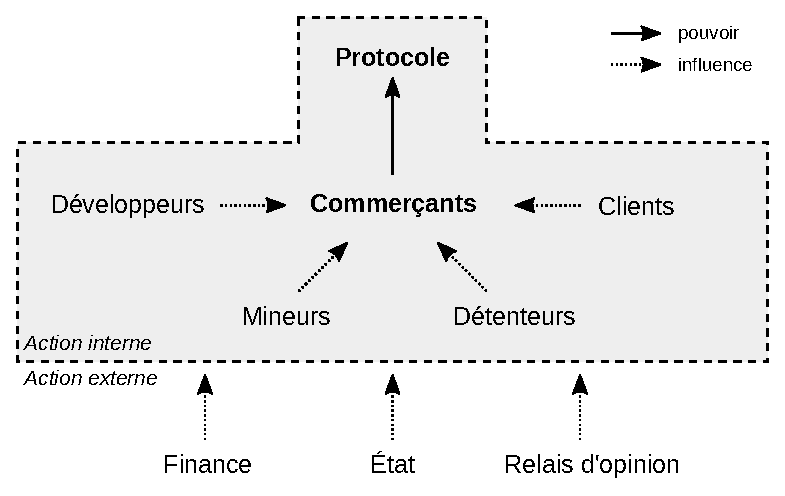
\includegraphics[scale=0.75]{img/bitcoin-governance-model.eps}
  \caption{Un modèle de gouvernance de Bitcoin~: interactions des principaux groupes d'acteurs dans la détermination du protocole.}
\end{figure}

\section*{L'influence des développeurs}
\addcontentsline{toc}{section}{L'influence des développeurs}

La première catégorie d'acteurs internes est formée des développeurs. Les développeurs sont les personnes qui travaillent directement au maintien et aux mises à niveau des implémentations complètes ou partielles du protocole. Ils œuvrent en particulier à la bonne santé de la chaîne par le biais des implémentations utilisées par les commerçants et par les mineurs. L'implémentation de référence, qui est la plus utilisée et qui sert de modèle aux autres implémentations, est la plus importante.

% Rôle d'intermédiaire entre les commerçants / mineurs et le protocole
Ce rôle d'intermédiaire leur confère une influence non négligeable sur les commerçants et les autres acteurs, qui ont rarement les capacités d'observer et de comprendre le code directement. De plus, le maintien d'un logiciel performant demande un travail coûteux qui ne peut pas être réalisé par n'importe qui. Cette situation leur donne une position de force dans la prise de décision sur le protocole.

% Consensus approximatif, consensus sommaire (rough consensus)
Les développeurs sont nombreux et possèdent diverses opinions. Pour remédier à ce problème, ils fondent souvent leur décision sur le concept de consensus approximatif (\eng{rough consensus}) qui n'est pas un consensus à proprement parler, mais l'estimation d'un sentiment de groupe ou d'une volonté générale. Ce recours au consensus approximatif permet en pratique d'obtenir une quasi unanimité sans qu'un élément individuel puisse perturber le processus\footnote{Ce concept de \eng{rough consensus} provient de son utilisation en 1998, par l'\eng{Internet Engineering Task Force} (IETF), qui le décrivait comme suit dans ses procédures pour les groupes de travail~: «~Les groupes de travail prennent des décisions au moyen d'un processus de “consensus approximatif”. Le consensus IETF ne requiert pas que chaque participant soit d'accord, bien que cela soit bien entendu préférable. De façon générale, l'opinion dominante du groupe de travail doit prévaloir (cependant, cette “dominance” ne doit pas être déterminée sur la base du volume ou de l'insistance, mais plutôt selon une impression plus générale d'accord). Le consensus peut être déterminé au moyen d'un vote à main levée, ou de n'importe quel autre moyen sur lequel le groupe de travail est d'accord. Il convient de noter que 51~\% des voix ne peut être considéré comme un “consensus approximatif”, et qu'en sens inverse, 99~\% est mieux qu'approximatif. C'est au président de déterminer si un consensus approximatif est atteint.~» -- \eng{IETF Working Group Guidelines and Procedures}, septembre 1998~: \url{https://datatracker.ietf.org/doc/html/rfc2418}.}. Cette façon d'exclure les éléments récalcitrants peut être critiquée (une personne peut avoir raison contre le groupe), mais elle a l'intérêt de préserver l'effet de réseau du protocole, en offrant une proposition unique aux commerçants. % logique sacrificielle, René Girard.

% Bitcoin Core
Pour BTC, l'implémentation de référence est Bitcoin Core, dirigée par des mainteneurs. Ces mainteneurs, et plus généralement les développeurs, sont vus comme les gardiens du protocole. L'utilisation d'une autre implémentation (\eng{fork}) est toujours possible mais est à la fois coûteuse et mal vue, de sorte qu'il existe une inertie jouant en faveur de Bitcoin Core.

% Il faut en convenir : les mainteneurs de Bitcoin Core possèdent effectivement une grande influence sur les règles de consensus de BTC, étant vus comme les gardiens du protocole. Cette situation a l'avantage d'apporter une grande stabilité en décourageant les dissidences au sein de Bitcoin et les scissions de chaîne qui pourraient en résulter (comme on l'a vu avec Bitcoin Cash et ses dérivés).

Cette dominance s'est manifestée au cours de l'histoire de Bitcoin par le rejet d'un certain nombre de dissidences, qui ont parfois donné lieu à la création d'une implémentation alternative. On peut citer~:

\begin{itemize}
\item Mike Hearn, qui, en 2014, voulait ajouter une requête de réseau \texttt{getutxos} à Bitcoin Core mais qui a été refusée pour cause de non-unanimité, ce qui a mené à la création de Bitcoin XT~;
\item Les partisans de l'augmentation de la limite de capacité transactionnelle du réseau durant la guerre des blocs, qui ont mis en place de multiples implémentations pour tenter, en vain, de faire adopter ce changement~: Bitcoin XT mi-2015, Bitcoin Classic début 2016, Bitcoin Unlimited mi-2016 et btc1 mi-2017~;
\item Les opposants à la mise à niveau SegWit, soutenue largement par Bitcoin Core, qui n'ont eu d'autre choix que de développer Bitcoin ABC, qui augmentait dans le même temps la taille limite des blocs, menant à la création de Bitcoin Cash~;
\item Jeremy Rubin, qui a menacé de faire activer le BIP-119 (soft fork) par les mineurs en 2022, en raison du refus de Bitcoin Core d'intégrer sa modification au logiciel, mais qui a fini par se raviser, ayant probablement obtenu l'attention qu'il désirait\pagenote{«~Jeremy Rubin, qui a menacé de faire activer le BIP-119 (soft fork) par les mineurs en 2022~»~: Jeremy Rubin, \eng{7 Theses on a next step for BIP-119}, 17 avril 2022~: \url{https://rubin.io/bitcoin/2022/04/17/next-steps-bip119/}~; archive~: \url{https://web.archive.org/web/20220419172825/https://rubin.io/bitcoin/2022/04/17/next-steps-bip119/}. -- On peut rapprocher son cas de celui de Paul Sztorc, qui travaille sur son concept de Drivechain depuis 2017, mais dont les propositions d'amélioration (BIP-300 et BIP-301) n'ont pas été intégrées par Bitcoin Core.}.
\end{itemize}

% Influence limitée des développeurs
Les développeurs, et notamment ceux de Bitcoin Core, exercent ainsi une influence importante sur le protocole. Cependant cette influence reste limitée~: dans le cas où ils s'opposeraient à l'économie de façon trop tranchée, ces derniers seraient remplacés par d'autres développeurs.

% Thankful_for_today, Monero
Le premier exemple d'une dissidence réussie se trouve dans l'histoire des débuts de Monero\footnote{dEBRUYNE, \eng{Re: Monero inception - how did bitmonero become monero?}, \wtime{11/08/2016 16:21}~: \url{https://monero.stackexchange.com/questions/1011/monero-inception-how-did-bitmonero-become-monero/1024\#1024}.}. Monero a été créé sous le nom de Bitmonero en avril 2014 par un développeur utilisant le pseudonyme thankful\_for\_today, dans le but de relancer le projet Bytecoin qui avait fait l'objet d'un préminage massif. Cependant, il s'est rapidement avéré que thankful\_for\_today, «~dictateur bienveillant~» autoproclamé, procédait à des changements sans consulter les autres personnes impliquées et il s'est donc vu être évincé du projet après quelques jours. Une équipe de six développeurs a alors décidé de forker le projet et de le renommer en Monero.

% Amaury Séchet, Bitcoin Cash
Le second exemple d'une dissidence réussie est l'opposition à Bitcoin ABC en 2020 dans le cadre du protocole Bitcoin Cash. Bitcoin ABC, l'implémentation de référence de Bitcoin Cash depuis 2017, avait pour développeur en chef, Amaury Séchet. En 2020, ce dernier a approuvé la suggestion des mineurs de procéder à un soft fork pour rediriger une partie de la récompense de bloc vers les équipes de développement\pagenote{«~la suggestion des mineurs de procéder à un soft fork pour rediriger une partie de la récompense de bloc vers les équipes de développement~»~: Jiang Zhuoer, \eng{Infrastructure Funding Plan for Bitcoin Cash}, 22 janvier 2020~: \url{https://medium.com/@jiangzhuoer/infrastructure-funding-plan-for-bitcoin-cash-131fdcd2412e}~; archive~: \url{https://web.archive.org/web/20200123082358/https://medium.com/@jiangzhuoer/infrastructure-funding-plan-for-bitcoin-cash-131fdcd2412e}.} et a fini en novembre par tenter d'imposer ce changement via une intégration dans Bitcoin ABC\pagenote{«~a fini en novembre par tenter d'imposer ce changement via une intégration dans Bitcoin ABC~»~: Amaury Séchet, \eng{Bitcoin ABC's plan for the November 2020 upgrade}, 6 août 2020~: \url{https://amaurysechet.medium.com/bitcoin-abcs-plan-for-the-november-2020-upgrade-65fb84c4348f}.}. Une implémentation alternative, Bitcoin Cash Node, a alors été créée pour faire face à ce changement\pagenote{«~Une implémentation alternative, Bitcoin Cash Node, a alors été créée pour faire face à ce changement~»~: Notamment grâce aux deux développeurs anonymes freetrader et imaginary\_username. -- freetrader, \eng{Bitcoin Cash Node}, 20 février 2020~: \url{https://read.cash/@freetrader/bitcoin-cash-node-662e4737}.}, et a recueilli une large majorité économique, devenant ainsi l'implémentation de référence de ce qu'on appelle toujours aujourd'hui Bitcoin Cash. L'application de la redirection de la subvention du protocole a mené à la création du protocole XEC.

Ainsi, l'influence des développeurs sur le protocole est réelle, mais elle est profondément limitée par l'intervention de l'économie si elle a lieu.

\section*{La pression des mineurs}
\addcontentsline{toc}{section}{La pression des mineurs}

La deuxième catégorie d'acteurs impliqués dans l'influence sur le protocole est constituée des mineurs. Les mineurs sont les personnes ou les groupes de personnes qui s'occupent de la confirmation des transactions grâce à la dépense énergétique liée à la preuve de travail. Comme montré dans le chapitre~\ref{ch:censure}, ils disposent d'un pouvoir de sélection sur les transactions, leur conférant par là, en cas de regroupement majoritaire, la possibilité de procéder à une double dépense ou d'appliquer une censure active.

% Pouvoir des mineurs en tant que commerçants
Contrairement à ce qu'on peut parfois s'imaginer, les mineurs n'ont de pouvoir direct sur le protocole que dans le sens où ils forment une catégorie particulière de commerçants. Ils interviennent dans l'économie en acceptant de confirmer des transactions en échange de frais. Mais ce pouvoir direct est extrêmement limité du fait de la petitesse de leur activité économique par rapport à l'activité totale.

% Influence par attaque, attaque de la chaîne concurrente
Il n'en reste pas moins que les mineurs possèdent une influence non négligeable dans la prise de décision, qui procède de leur pouvoir d'attaque sur le consensus. D'une part, les mineurs peuvent influer dans le choix de l'économie lors d'une scission en attaquant la branche concurrente dans le but de la discréditer. C'est ce qu'ont menacé de faire les mineurs pro-BSV en novembre 2018 suite à la séparation avec BCH\footnote{Une «~guerre du hachage~» s'est déroulée entre les mineurs de Bitcoin SV, soutenus par Craig Wright et Calvin Ayre, et ceux de Bitcoin ABC, soutenus par Roger Ver et Jihan Wu, notamment par la redirection de la puissance de calcul de leurs coopératives de minage respectives. -- Aaron van Wirdum, \eng{Week 2: How the Bitcoin Cash "Hash War" Came and Went and Not Much Happened}, 30 novembre 2018~: \url{https://bitcoinmagazine.com/technical/week-2-how-bitcoin-cash-hash-war-came-and-went-and-not-much-happened}.}. C'est également ce qu'a fait le mineur pro-BCHN face à Bitcoin ABC en novembre 2020 en censurant la chaîne de Bitcoin ABC\pagenote{«~C'est également ce qu'a fait le mineur pro-BCHN face à Bitcoin ABC en novembre 2020 en censurant la chaîne~»~: \url{https://decrypt.co/49819/bitcoin-cash-rebels-launch-51-attack-to-destroy-bch-hard-fork}.}.

% Soft fork
D'autre part, les mineurs peuvent influencer le choix de l'économie en imposant un soft fork qui, dans son application, est indiscernable de la censure. L'ensemble des règles de consensus initial reste le même, mais ne peut plus s'exprimer pleinement, à tel point que cela peut induire les commerçants à adopter le soft fork en arrêtant d'accepter les transactions et les blocs qui ne s'y conforment pas. C'est ce que le développeur Peter Todd a décrit comme un «~soft fork forcé\footnote{Peter Todd, \eng{Forced Soft Forks}, 18 janvier 2016~: \url{https://petertodd.org/2016/forced-soft-forks}.}~» ou que d'autres appellent un «~fork maléfique\pagenote{«~fork maléfique~»~: \url{https://www.reddit.com/r/Bitcoin/comments/3yrsxt/bitcoindev_an_implementation_of_bip102_as_a/cyg4m39/}.}~» (\eng{evil fork}). La situation peut être résolue de deux manières~: ou bien les commerçants continuent d'appliquer les anciennes règles et créent par là un différentiel de frais encourageant les mineurs à revenir à la normale~; ou bien ils conviennent d'adopter un hard fork annulant ce soft fork, prenant alors le risque de la spirale de scissions liée à l'intervention humaine rapide.

% Influence limitée des mineurs, gouvernance par preuve de travail
Toutefois, cette influence des mineurs s'arrête là. Les commerçants continuent de déterminer les règles et les mineurs sont impuissants face à cette réalité. Il est donc faux de prétendre que les mineurs sont les maîtres du protocole (gouvernance par preuve de travail), comme le faisaient une bonne partie des \eng{big blockers} durant la guerre des blocs\footnote{C'était, par exemple, la conception du PDG de Coinbase, Brian Armstrong, qui écrivait le 3 janvier 2016~: «~Heureusement, Bitcoin dispose d'un mécanisme de mise à niveau intégré et élégant. Si la majorité des mineurs de Bitcoin “votent” pour une mise à niveau particulière, il s'agit par définition de la nouvelle version de Bitcoin. Le nombre de votes obtenus par chaque mineur est proportionnel à la quantité de puissance de calcul qu'il apporte au réseau (les votes ne peuvent donc pas être truqués).~» -- Brian Armstrong, \eng{Scaling Bitcoin: The Great Block Size Debate}, 3 janvier 2016~: \url{https://www.coinbase.com/blog/scaling-bitcoin-the-great-block-size-debate}.}. En effet, si c'était réellement le cas, alors le système économique de Bitcoin serait voué à l'échec, les mineurs étant naturellement incités à augmenter leurs revenus par l'inflation, à l'instar des banques centrales.

\section*{L'importance des utilisateurs}
\addcontentsline{toc}{section}{L'importance des utilisateurs}

La troisième catégorie d'acteurs internes ayant une influence sur le protocole est la catégorie des utilisateurs non commerçants. Les utilisateurs sont souvent mis en avant comme les personnes ayant le dernier mot sur le protocole\footnote{«~Le réseau Bitcoin n'appartient à personne, tout comme la technique derrière le courriel n'appartient à personne. Bitcoin est contrôlé par l'ensemble de ses utilisateurs autour du monde. Alors que les développeurs améliorent les logiciels, ils ne peuvent pas imposer de modification dans le protocole Bitcoin parce que chaque utilisateur est libre de choisir quel logiciel et quelle version il utilise. Afin de rester compatibles avec les autres, tous les utilisateurs doivent utiliser des logiciels se conformant aux mêmes règles. Bitcoin ne peut fonctionner correctement qu'avec un consensus total entre ses utilisateurs.~» -- Bitcoin.org FAQ~: \url{https://bitcoin.org/fr/faq\#qui-controle-le-reseau-bitcoin}.}. Toutefois, le terme d'utilisateur est ambigu et peut prêter à confusion, car l'utilisation du bitcoin englobe généralement trois actions distinctes~: l'acceptation dans le commerce, la détention durant une période donnée et la dépense auprès d'autres personnes. De là, on peut dégager trois sous-catégories théoriques d'utilisateurs~: les commerçants, les clients et les détenteurs. La première possède le pouvoir effectif sur le protocole, tandis que les deux autres n'exercent qu'une simple influence.

% --- Les clients ---

Parlons d'abord des clients, qui sont les personnes qui échangent leurs bitcoins contre des biens et services dans le commerce, y compris d'autres monnaies. Ils sont le pendant des commerçants, l'échange étant par définition symétrique~: sans client (acheteur), il n'y a pas de commerçant (vendeur), et vice versa. Il y a donc une interdépendance entre les commerçants et les clients. % De plus, il faut avoir été préalablement un commerçant avant de devenir un client, sauf si on nous a donné des bitcoins.

% Influence des clients
Dans la détermination du protocole, les clients exercent par conséquent une très grande influence. Un commerçant, s'il veut continuer à prospérer dans les affaires, devra choisir d'accepter (au moins) la monnaie liée au protocole soutenu majoritairement par ses clients. L'histoire du refus de SegWit2X en 2017 est l'exemple parfait de l'influence des clients, où les utilisateurs ont réussi à influencer les plus gros commerçants (les plateformes de change) et à les pousser à renoncer au doublement de la taille limite des blocs en novembre\pagenote{Satoshi Nakamoto, \eng{Re: BitDNS and Generalizing Bitcoin}, \wtime{10/12/2010 17:29:28 UTC}, \url{https://bitcointalk.org/index.php?topic=1790.msg28917\#msg28917}~: «~Les utilisateurs de Bitcoin pourraient devenir de plus en plus sectaires à propos de la limitation de la taille de la chaîne pour que son accès reste facile pour beaucoup d'utilisateurs et pour les petits appareils.~»}.

% Limite de l'influence des clients
Toutefois, l'idée que ces clients partagent la maîtrise du protocole avec les commerçants est erronée. Si la dissension est équilibrée parmi les utilisateurs, alors c'est le commerçant qui tranche en optant pour un protocole plutôt que l'autre pour offrir ses biens et services à des prix acceptables. Au bout du compte, le client (qui se débarrasse de ses bitcoins) n'apporte aucune utilité à la monnaie~; le commerçant, si.

% --- Les détenteurs ---

Considérons ensuite les détenteurs, c'est-à-dire les personnes qui conservent des bitcoins en réserve durant une période significative. Ces détenteurs sont parfois appelés thésauriseurs\pagenote{«~appelés thésauriseurs~»~: Daniel Krawisz, \eng{I'm Hoarding Bitcoins, and No You Can't Have Any}, 12 février 2014~: \url{https://nakamotoinstitute.org/mempool/im-hoarding-bitcoins-and-no-you-cant-have-any/}.} ou HODLers (par déformation du verbe \eng{to hold}, «~garder~», «~conserver~»\footnote{GameKyuubi, \eng{I AM HODLING}, \wtime{18/12/2013 10:03:03 UTC}~: \url{https://bitcointalk.org/index.php?topic=375643.msg4022997\#msg4022997}.}) pour insister sur le fait qu'ils ne veulent pas se séparer de leurs bitcoins de sitôt. Par cette action, ils restreignent l'offre de monnaie à proprement parler ce qui, conjugué à une demande plus forte, a un effet haussier sur le pouvoir d'achat de l'unité et sur son taux de change avec le dollar, communément appelé «~le prix~».

% Influence des détenteurs
Les détenteurs ont une influence sur les commerçants. Premièrement, par leur épargne, ils augmentent la taille de la subvention du protocole, et donc le budget du minage pour la protection contre la double dépense, assurant une plus grande sécurité aux commerçants. Deuxièmement, la détention offre au marché plus de liquidité potentielle, ce qui permet à des utilisateurs plus importants d'entrer. Troisièmement, un prix plus haut a un effet de communication non négligeable, notamment par l'attention qu'un engouement spéculatif entraîne dans les médias. Ainsi, si une scission a lieu, les détenteurs peuvent vendre la monnaie d'une branche contre celle de l'autre et créer un différentiel favorable au protocole privilégié (c'est ce qui s'est passé durant la scission entre BTC et BCH).

% Gouvernance par preuve d'enjeu
La conception selon laquelle le pouvoir d'achat de la monnaie serait primordial a poussé certains protocoles cryptoéconomiques comme Dash et Tezos à innover en créant des systèmes de gouvernance internes permettant de résoudre les disputes à propos de la modification du protocole par un vote proportionnel à la possession d'unités (gouvernance par preuve d'enjeu). Les détenteurs seraient assimilés aux parties prenantes d'une société, possédant des parts dans cette dernière, qui serait essentiellement une organisation autonome décentralisée (DAO).

% Limite de l'influence des détenteurs
Toutefois, cette conception ne tient que dans la phase précoce de Bitcoin, où la création monétaire forme l'essentiel du revenu minier, où l'activité est encore hautement spéculative (l'achat et la vente de monnaie fiat dans le but d'en tirer un profit) et où les principaux commerçants sont les plateformes de change et leurs utilisateurs. À long terme, la diminution de la subvention minière et la stabilisation réduit cet effet et donne un rôle beaucoup plus important aux transactions non spéculatives, car s'il existe une relation entre l'utilité et le prix de l'unité, c'est la première qui prime sur le second.

Ainsi, l'influence générale des acteurs internes sur les commerçants -- développeurs, mineurs, clients et détenteurs -- est non négligeable et joue un rôle dans la détermination du protocole. Mais ce n'est pas la seule pression qui s'exerce, et il faut aussi compter les acteurs externes au système, qui participent aussi à leur niveau dans le mécanisme de gouvernance.

\vspace{-1em}
\section*{Le poids des relais d'opinion} % Cœurs
\addcontentsline{toc}{section}{Le poids des relais d'opinion}

La première catégorie des influences extérieures est celle des relais d'opinion, qui orientent l'avis des personnes actives dans Bitcoin. Ces relais peuvent être individuels (influenceurs) ou collectifs (médias). La raison de leur existence est qu'il est impossible de saisir par soi-même toutes les subtilités de Bitcoin, de sorte que la plupart des utilisateurs se contentent souvent d'une explication rudimentaire proposée par autrui, et font reposer un partie de leur jugement sur la confiance accordée à autrui.

% Meneurs
Cette situation conduit à l'émergence d'acteurs plus influents que les autres, par leur prestige individuel ou par les médias qu'ils dirigent. On dit parfois que Bitcoin n'a pas de chef, de meneur, qu'il est acéphale\footnote{Le terme de «~monnaie acéphale~» a été popularisé par Jacques Favier et Adli Takkal Bataille dans \emph{Bitcoin, la monnaie acéphale} en 2017.}. Cependant, force est de constater que ce n'est pas le cas \emph{stricto sensu} et que certaines personnes ont un poids plus important que d'autres dans la prise de décision, indépendamment de leur activité économique.

% Experts techniques
D'abord, les experts techniques, qui sont censés mieux connaître les méandres du protocole que les autres, rentrent dans cette catégorie. Ils peuvent être développeurs eux-mêmes, avoir une activité proche, ou bien être éducateurs ou rédacteurs. Nous pouvons par exemple citer Adam Back, ancien cypherpunk et PDG de Blockstream, Andreas Antonopoulos, éducateur de longue date, ou encore Aaron van Wirdum, rédacteur expérimenté pour le Bitcoin Magazine et coanimateur du podcast Bitcoin Explained.

% Politiques et économistes
Ensuite, viennent les acteurs impliqués politiquement qui saisissent les intérêts profonds de Bitcoin. On peut mentionner ici l'activiste Alex Gladstein, directeur de la stratégie à la Human Rights Foundation. Puis viennent les économistes, qui comprennent mieux que les autres les mécanismes économiques à l'œuvre dans Bitcoin, comme l'économiste et auteur Saifedean Ammous, l'experte en macroéconomie Lyn Alden, ou encore le magistrat financier Yorick de Mombynes en France.

% Financiers
Enfin, nous avons les financiers, qui ont fait fortune avant de découvrir Bitcoin ou bien grâce à lui. Ces personnes sont considérées comme des modèles du fait de leur réussite financière, qui est l'objectif principal de la majorité des gens qui s'intéressent à Bitcoin en premier lieu. Roger Ver, les frères Winklevoss et Michael Saylor en font partie. On peut aussi citer le milliardaire Elon Musk, qui est l'archétype de ce type d'influence, et qui a notamment donné une seconde vie à Dogecoin en le citant à de multiples reprises dans ses interventions publiques.

% Médias
Toutes ces personnalités sont souvent relayées par les médias, qui jouent eux-même un rôle de relai d'opinion. Ces derniers exercent en effet une certaine influence en choisissant quels contenus sont publiés ou diffusés et lesquels ne le sont pas. Ils permettent au grand public qui n'a pas le temps ou l'envie de lire sur le sujet de se forger un avis.

% Médias spécialisés
Il peut s'agir des vidéastes individuels qui produisent du contenu sur les cryptomonnaies, notamment sur la plateforme Youtube. Il y a aussi les autres médias spécialisés comme les sites d'information (Bitcoin.org, Bitcoin.fr), les médias d'actualité (Bitcoin Magazine, Cointelegraph, Coindesk, Bitcoin.com à l'international~; Cryptoast et le Journal du Coin en France), les chaînes vidéo (Grand Angle Crypto), les podcasts, les lettres d'information payantes (The Big Whale). On peut également mentionner les plateformes de discussion spécialisées, dont le forum de discussion historique bitcointalk.org, les subreddits consacrés à Bitcoin (r/bitcoin, r/btc), et aujourd'hui les groupes Telegram dédiés.

% Médias généralistes
Les médias généralistes exercent aussi une influence, bien qu'elle soit encore plus diffuse. C'est par exemple le cas des chaînes d'informations financières (CNBC, BFM Business) qui consacrent parfois des émissions au sujet des crypto-actifs. On peut aussi citer tous les médias sociaux qui peuvent modeler l'opinion publique à propos de Bitcoin, comme c'est le cas de Twitter, lieu privilégié pour la communication sur Bitcoin\pagenote{«~Twitter, lieu privilégié pour la communication sur Bitcoin~»~: Cette dépendance à Twitter a poussé les bitcoineurs à développer leur propre protocole de média social décentralisé~: Nostr.}.

\vspace{-1em}
\section*{La puissance suggestive de la finance} % Carreaux
\addcontentsline{toc}{section}{La puissance suggestive de la finance}

Le discours n'est cependant pas la seule manière d'influencer les acteurs du système~: il existe également le «~pouvoir~» de l'argent. Les puissances financières jouent un rôle dans la détermination du protocole en choisissant de financer l'écosystème et les influenceurs de la variante de Bitcoin qui leur plaît. Elles peuvent par exemple fournir des fonds pour la croissance commerciale (listage sur plateforme de change), le développement logiciel, la création d'applications innovantes, le marketing, le lobbying auprès des instances régulatrices, etc.

% Financement des développeurs
Le financement de l'implémentation de référence est particulièrement crucial. L'infrastructure logicielle n'est pas maintenue gratuitement, mais elle n'apporte aucun revenu, du fait de l'absence nécessaire de contrainte légale sur son utilisation. C'est pourquoi les développeurs doivent trouver de l'argent quelque part\footnote{Divers modèles de financement ont été proposés~: celui de la Fondation Bitcoin entre 2012 et 2014, celui du capital-risque avec le financement de Blockstream à partir de 2014, celui du financement participatif avec Lighthouse (BTC) en 2014 et Flipstarter (BCH) en 2020, et enfin celui de l'utilisation de la subvention de minage (Dash, Zcash, XEC) depuis 2015.}. C'est ainsi que diverses organisations financent le développement~: en 2023, le salaire versé aux personnes chargées de l'écriture et de la révision du code dans Bitcoin Core provient principalement (par ordre d'importance) de l'organisation caritative Brink (elle-même financée par les principales plateformes de change), la \eng{Digital Currency Initiative} du MIT Media Lab, le groupe de développement et de recherche Chaincode Labs, l'entreprise Block de Jack Dorsey et la plateforme de trading sur marge BitMEX\pagenote{«~le salaire versé aux personnes chargées de l'écriture et de la révision du code dans Bitcoin Core provient principalement~»~: \url{https://blog.bitmex.com/wp-content/uploads/2022/10/Bitcoin-Grant-Presentation-1.pdf}}.

% Blockstream, Digital Currency Initiative
Cela donne aux puissances financières une influence particulière, chose qui a été dénoncée au sujet de Blockstream depuis ses débuts, l'entreprise ayant notamment reçu un investissement de la part d'AXA. On peut aussi citer le cas de la \eng{Digital Currency Initiative} dont le rôle est plus qu'ambigu. Cette entité a en effet été l'organisation en charge du développement du prototype de monnaie numérique de banque centrale des États-Unis tout en continuant de payer le mainteneur principal de Bitcoin Core, Wladimir van der Laan.

\vspace{-1em}
\section*{La guerre de l'État contre le protocole} % Piques, influence étatique
\addcontentsline{toc}{section}{La guerre de l'État contre le protocole}

Pour finir, la troisième et dernière méthode utilisée pour influencer les acteurs du système et donc le protocole, c'est la force, ou plus précisément la menace d'utiliser la force, une spécialité largement monopolisée par une grande institution appelée l'État.

% Rapport antagoniste avec Bitcoin
L'existence de l'État est profondément liée au contrôle sur la monnaie, qui facilite grandement la collecte de son revenu. En particulier, il prélève un seigneuriage grâce à la domination qu'il exerce sur la détermination du support monétaire. De ce fait, il existe un rapport antagoniste entre l'État et Bitcoin, ce dernier redonnant aux individus la maîtrise totale de leur monnaie. % incarnation principale du transfert de richesse non consenti

% Influence sur le protocole Bitcoin
Il est donc logique que l'État cherche à influencer l'évolution du protocole, voire qu'il finisse par tenter de le décréter. Par la définition du cadre légal, il peut en effet influer sur le choix des commerçants. Son pouvoir politique n'est cependant pas illimité. S'il s'y prend mal ou si le changement est trop brutal, ces commerçants risquent de désobéir en masse et de rejoindre le marché noir, où aucune autorisation n'est requise.

C'est le pouvoir économique qui détermine le protocole en dernier lieu. Mais avec le temps l'État peut s'immiscer dans ses décisions pour altérer doucement les propriétés de Bitcoin. Par des lois intelligentes, il peut faire en sorte que son action reste largement acceptée et qu'une bonne partie de l'économie continue d'avoir lieu sur le marché réglementé. Il peut aussi influencer les différents acteurs qui jouent un rôle dans le modèle de gouvernance de Bitcoin, comme les développeurs, les mineurs ou les médias, sans que ceux-ci ne réagissent.

% Réglementations
Les réglementations financières constituent des étapes préparatoires dans le déploiement d'une telle influence. Il s'agit des contraintes imposées aux plateformes de change (commerçants principaux) qui se chargent d'effectuer la jonction entre le bitcoin et les monnaies officielles. Initiées en 2013, ces réglementations imposent aujourd'hui une procédure de connaissance du client (KYC) et de connaissance des transactions (KYT) assez drastique, de sorte que l'anonymat dans ce type d'échange devient de plus en plus difficile à préserver. Elles ont le double avantage d'habituer les acteurs économiques à se conformer et de restreindre leur nombre en requérant des contraintes de plus en plus insurmontables pour les plus petites plateformes. Ces réglementations peuvent également s'appliquer aux commerçants en général. De plus, la loi les contraint déjà dans la plupart des juridictions à déclarer leurs plus-values par rapport à la monnaie nationale, ce qui complique leur activité.

% Interdiction pure et simple
Voyons maintenant comment le protocole pourrait être attaqué. Tout d'abord, l'acceptation du bitcoin pourrait être rendue illégale, sans alternative. Toute l'économie portée par les commerçants du marché réglementé serait détruite d'un simple trait de plume. L'utilité du système serait alors grandement réduite sur le moment, ainsi que la valeur d'échange de l'unité de compte.

Ce type d'interdiction totale a déjà eu lieu dans certains pays, comme le Maroc, l'Algérie, la Bolivie ou le Népal. D'autres pays ont choisi d'interdire uniquement une section de l'économie, que ce soit le change avec la monnaie nationale (Chine), la vente de biens et services sur le territoire (Turquie, Équateur, Thaïlande) ou l'acquisition par des acteurs financiers (Iran, Nigéria). Toutefois, sauf dans le cas de la Chine, ces interdictions n'ont pas été réalisées par des puissances majeures, de sorte que l'utilisation du bitcoin reste légale sur la majorité de la planète. Une réelle interdiction, si elle avait lieu, aurait besoin de se faire de manière internationale pour avoir une influence réelle et amoindrir l'utilité de Bitcoin.

L'impact de cette interdiction pure et simple est difficile à mesurer. En effet, on peut douter de la capacité d'application de ces lois. Une interdiction sans soutien populaire aurait pour conséquence d'accroître la taille du marché noir. De ce fait, il semble évident qu'une telle attaque s'accompagnerait de la proposition d'une alternative contrôlée de Bitcoin ayant pour but de contenter la partie la plus «~pragmatique~» de l'économie.

% Altération du protocole
Dans le but de s'opposer à Bitcoin, l'État pourrait ainsi déployer sa propre version du protocole dans le but de ronger progressivement les propriétés fondamentales de Bitcoin. Cette version altérée de Bitcoin serait rendue légale et bénéficierait d'un régime accommodant, tandis que la version originelle serait rendue illégale. Les acteurs conformistes seraient récompensés à court terme par une augmentation du prix, alors que les commerçants dissidents seraient punis par des amendes et des peines de prison.

% Soft forks de censure
En premier lieu, des soft forks de censure pourraient être appliqués en se basant sur les normes générales de LCB-FT. Ceux-ci pourraient s'accompagner d'une attaque de censure active par les mineurs. Les acteurs conformistes pourraient justifier leur choix en disant que ces transactions n'ont rien à faire sur la chaîne de Bitcoin.

% Soft forks de censure totale
En deuxième lieu, un soft fork pourrait aller jusqu'à concerner toutes les transactions, en requérant une autorisation étatique pour chacune d'entre elles. À ce stade, les plus conformistes pourraient toujours s'imaginer que la politique monétaire aurait été préservée.

% Soft fork taxatoire
En troisième lieu, un soft fork taxatoire pourrait être mis en place. Celui-ci consisterait à prélever une taxe fixe sur toutes les transactions, dans l'idée de la TVA, ou bien à extraire un demeurage, en soustrayant un montant dépendant du temps de détention des fonds dépensés. Ces impôts pourraient être réalisés dans l'objectif de réguler la nature trop déflationniste du bitcoin et la répartition inique de la richesse.

% Hard fork d'inflation
En quatrième lieu, un hard fork d'inflation pourrait être appliqué. À ce stade, les acteurs restants n'auraient plus rien à voir avec les acteurs originaux. Ce qui faisait la renommée de «~Bitcoin~» serait alors totalement anéanti, et le système correspondant ressemblerait trait pour trait à une monnaie numérique de banque centrale.

% Résistance
Ce scénario, bien qu'hypothétique, forme la conséquence logique de l'influence de l'État sur la monnaie et est donc inévitable jusqu'à un certain point. Toutefois, il suppose dans le même temps le développement d'une économie parallèle dans laquelle l'acceptation du bitcoin se ferait de manière clandestine. Face à la censure de plus en plus forte, il se formerait ainsi une opposition, une résistance. Les altérations progressives rendraient la chaîne officielle de moins en moins utile, en faisant fuir les commerçants ne souhaitant pas se conformer.

À un certain moment, une scission aurait lieu. La version étatique pourrait être minoritaire, auquel cas elle se séparerait naturellement de l'autre chaîne (scénario optimiste). Mais elle pourrait aussi être majoritaire, auquel cas la version clandestine serait contrainte de procéder à un hard fork pour subsister (scénario pessimiste). Dans les deux cas, la reconstruction de Bitcoin se produirait alors à partir de la chaîne libre, au sujet de laquelle il n'y aurait aucune ambiguïté au niveau du protocole. Cette chaîne pourrait cependant être attaquée du point de vue minier, ce que nous avons décrit en détail dans le chapitre~\ref{ch:censure}.

\vspace{-1em}
\section*{Deux niveaux de sécurité}
\addcontentsline{toc}{section}{Deux niveaux de sécurité}

Bitcoin est un concept de monnaie numérique résistante à la censure et à l'inflation. Ces deux propriétés fondamentales sont complémentaires, mais elles nécessitent des sécurités différentes. La résistance à la censure repose sur la sécurité minière~; la résistance à l'inflation sur la sécurité commerciale.

La détermination du protocole -- ou plutôt des protocoles puisqu'il peut y en avoir plusieurs -- est réalisée par les commerçants au sens large, c'est-à-dire les personnes qui acceptent le bitcoin dans l'échange contre des biens, des services ou d'autres monnaies. Les commerçants vérifient les règles de consensus par l'intermédiaire de leurs nœuds. Ce pouvoir sur le protocole est proportionnel à l'activité économique potentielle du commerçant, qui peut être estimée par ses recettes effectives. Il dépend aussi de l'effet de réseau qui fait que l'utilité combinée apportée par les commerçants va évoluer de manière superlinéaire.

Un certain nombre d'influences s'exercent sur les commerçants pour qu'ils acceptent tel ou tel protocole. S'il est dur de comprendre comment cet ensemble complexe interagit, il est possible d'en dessiner les contours comme nous l'avons fait ici. En particulier, l'influence majeure à ne pas négliger est celle de l'État, qui pourrait attaquer le protocole en bonne et due forme par la coercition des commerçants et des autres acteurs.

Pour que le protocole de Bitcoin soit réellement robuste, il faut donc que l'activité économique soit décentralisée, à l'instar du minage~: que les commerçants (ou petits groupes de commerçants) fassent fonctionner leurs propres nœuds pour que, dans l'hypothèse d'un changement des règles décrété par une autorité, les risques soient répartis dans l'économie et que Bitcoin puisse continuer à survivre clandestinement.

Il est nécessaire que l'accord sur le protocole s'exerce à long terme. La courte histoire de Bitcoin regorge de multiples perturbations qui montrent que le changement des règles de consensus ne se passe pas toujours dans les meilleures conditions. Seul le temps permet de faire le tri entre les bonnes modifications et les mauvaises.


% \part{Comment ?}

% Copyright (c) 2022 Ludovic Lars
% This work is licensed under the CC BY-NC-SA 4.0 International License

\chapter{Les rouages de la machine}
\label{ch:rouages}

Bitcoin est une étrange machine. Né dans un contexte antagoniste vis-à-vis de l'autorité, il possède des propriétés qui ne se retrouvent pas dans les systèmes informatiques communs. En particulier, il ne peut pas être modifié n'importe comment, ce qui explique sa conception de base et son évolution.

D'une part, la représentation des unités de base, les satoshis, ne se fait pas au travers de comptes sur lesquels les soldes des utilisateurs seraient mis à jour, mais par des pièces de cryptomonnaies pouvant être combinées et séparées dans les transactions. Ce fonctionnement est important à comprendre pour bien saisir comment la confidentialité est possible sur la chaîne.

D'autre part, Bitcoin intègre un système de programmation interne permettant d'implémenter des conditions de dépense dans les pièces. Ce système a été amélioré au cours des années, parfois au prix d'une plus grande complexité, notamment via l'ajout de SegWit et de Taproot.

\section*{Les transactions et les pièces} % Modèle de représentation par des pièces
\addcontentsline{toc}{section}{Les transactions et les pièces}

% Transactions
Dans Bitcoin, les transactions possèdent un rôle central. Le protocole est fait pour échanger de la valeur conformément à son rôle monétaire, donc de traiter les transferts de propriété. Tout le fonctionnement du système a été pensé pour faciliter la construction, la signature et la diffusion des transactions, leur conservation en mémoire dans la \eng{mempool}, et leur ajout au registre par l'intermédiaire de leur inclusion dans un bloc.

% Entrées et sorties
Chaque transaction est constituée d'une ou plusieurs entrées et d'une ou plusieurs sorties. Une sortie transactionnelle se compose simplement d'une indication de destination et d'un montant en unités (satoshis). Une entrée fait généralement référence à une sortie transactionnelle précédente, sauf dans le cas de la transaction de récompense où elle constitue une «~base de pièce~» créant de nouvelles unités issues de l'émission monétaire et des frais de transaction. % par une indication de provenance composée de l'identifiant de la transaction précédente et de la position de la sortie dans cette transaction.

% Identifiant et indice
L'identifiant d'une transaction (\eng{transaction identifier} ou \texttt{txid}) est l'empreinte des données brutes qu'elle contient, obtenue via le hachage par double SHA-256. Chaque sortie transactionnelle est caractérisée par l'identifiant de la transaction dont elle est issue et par sa position dans cette transaction, qu'on appelle l'indice. Ce point de sortie (\eng{outpoint}) sert d'indication de provenance. Un exemple de point de sortie est \texttt{\longstring{f4184fc596403b9d638783cf57adfe4c75c605f6356fbc91338530e9831e9e16:0}}.

% Scripts de verrouillage
Contrairement à ce que la description de la propriété dans le chapitre~\ref{ch:propriete} suggère, la destination et la provenance des unités ne sont pas à proprement parler des adresses, mais des scripts de verrouillage, c'est-à-dire des petits programmes qui déterminent leurs conditions de dépense. Chaque sortie crée ainsi un script de verrouillage qui bloque les fonds d'une façon spécifique. Le plus souvent, ce script contient une clé publique ou une empreinte de clé publique, qui peut être interprétée comme une adresse par le portefeuille.

% Scripts de déverrouillage
Pour être valide, une entrée doit contenir un script de déverrouillage dont l'exécution combinée à celle du script de verrouillage réussisse. En général, ce script contient une signature numérique qui correspond à la clé publique liée au script de verrouillage précédent~: la vérification de la signature permet de s'assurer que la personne qui dépense les fonds en est le propriétaire.

% Modèle de représentation par des comptes
Ce fonctionnement fait que le modèle de représentation des unités est contre-intuitif. Le protocole ne voit pas des comptes dont les soldes seraient actualisés par les transactions, comme c'est le cas dans Ethereum par exemple. Il voit simplement des sorties transactionnelles détenues par des propriétaires, de manière similaire aux pièces de monnaies dans le monde physique.

% Pièce de monnaie numérique
De ce fait, Bitcoin met en œuvre le concept de pièce de monnaie numérique qui était discuté au sein de la communauté cypherpunk dans les années 1990. Tim May estimait que la chose était impossible, en raison du problème de la double dépense\sendnote{«~Est-il possible de concevoir une "pièce de monnaie numérique"~? - La réponse semble être "non".~» -- Timothy C. May, \eng{Cyphernomicon}, 12.3.8.}. Satoshi Nakamoto, en découvrant une manière de résoudre ce problème, a pu rendre le concept viable et l'a intégré dans Bitcoin. Dans le livre blanc, il décrivait la pièce numérique comme suit~:

\begin{quote}
«~Nous définissons une pièce de monnaie électronique comme une chaîne de signatures numériques. Chaque propriétaire transfère la pièce au suivant en signant numériquement l'empreinte de la transaction précédente et la clé publique du propriétaire suivant, et en les ajoutant à la fin de la pièce. Un bénéficiaire peut vérifier les signatures pour vérifier la chaîne de propriété.\sendnote{Satoshi Nakamoto, \eng{Bitcoin: A Peer-to-Peer Electronic Cash System}, 31 octobre 2008.}~»
\end{quote}

% UTXO, UTXO set, état
Dans Bitcoin, les pièces existantes sont donc les sorties transactionnelles non dépensées, aussi abrégées en UTXO pour \eng{Unspent Transaction Outputs} en anglais, à savoir les sorties transactionnelles qui n'ont pas été utilisée comme entrée dans une autre transaction. L'ensemble de ces pièces, l'\eng{UTXO set}, constitue le registre de propriété. C'est l'état du système, qui peut être récupéré à partir de son historique, la chaîne de blocs.

% Pièce
Chaque pièce est constituée d'un montant en unités (satoshis) et d'un script de verrouillage. Il peut ainsi exister des pièces de 1~000~000~000~satoshis (10 bitcoins) tout comme on peut avoir des pièces de 546~satoshis (0,00000546 bitcoin).

% Adresses, comptes
Le script de verrouillage d'une pièce contient le plus souvent une clé publique ou une empreinte déterminée, de sorte que la pièce peut être vue comme étant détenue par l'adresse correspondante. De ce fait, deux pièces partageant le même script de verrouillage sont détenues par la même adresse. Un compte dans Bitcoin correspond à l'ensemble des adresses contrôlées par un utilisateur. Le solde est récupéré en balayant l'ensemble des UTXO de façon à retrouver les pièces détenues par ces adresses.

\begin{figure}[ht]
  \centering
  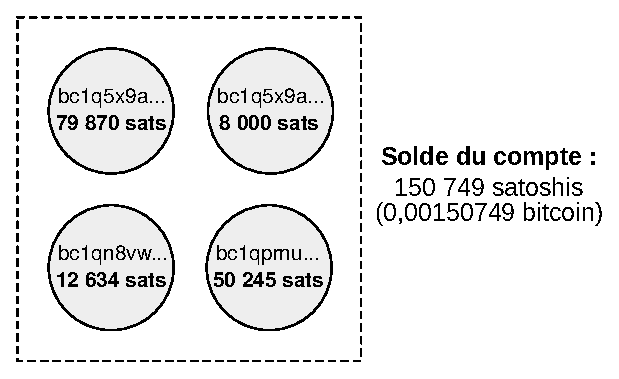
\includegraphics[scale=0.75]{img/coins-utxos-account.eps}
  \caption{Exemples de pièces détenues par un même compte.}
  \label{fig:coins-utxos}
\end{figure}

% Fonderie
Ce modèle de représentation par des pièces fait qu'on peut voir le mécanisme de transaction comme une fonderie de pièces de monnaie. Chaque transaction consiste à fondre ensemble une ou plusieurs pièces de bitcoin en entrée et à frapper une ou plusieurs pièces en sortie. C'est en ceci que le serveur d'horodatage distribué vient remplacer la monnaierie numérique centralisée qui permet le remplacement systématique des pièces, comme dans eCash et RPOW par exemple. %\sendnote{Voir chapitre~\ref{ch:cypherpunks}.}.

% Construction
La construction d'une transaction implique de rassembler des pièces de valeur suffisante en entrée pour les fondre et en frapper de nouvelles. En général, deux pièces sont créées~: la première est créée sur l'adresse fournie par le destinataire pour effectuer le paiement (sortie principale) et le seconde est créée sur l'une des adresses de l'expéditeur afin qu'il se «~rende la monnaie~» (sortie complémentaire). La différence entre le montant en entrée et le montant en sortie est prise en compte dans la récompense du mineur en tant que frais de transaction.

% Transaction à 1 entrée et 2 sorties
Considérons quelques exemples en ignorant ces frais et supposons qu'Alice veuille procéder à un paiement. Si Alice possède une pièce de 12~mBTC et veut donner 7~mBTC à Bob, alors elle doit construire et signer une transaction ayant pour entrée cette pièce de 12~mBTC et pour sorties une pièce de 7~mBTC vers l'adresse de Bob et une pièce restante de 5~mBTC vers sa propre adresse. Cette transaction est illustrée par la figure~\ref{fig:transaction-1i-2o}.

\begin{figure}[ht]
  \centering
  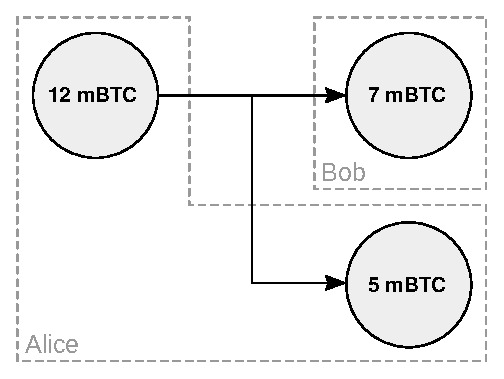
\includegraphics[scale=0.75]{img/transaction-1i-2o.eps}
  \caption{Schéma d'une transaction à 1 entrée et 2 sorties.}
  \label{fig:transaction-1i-2o}
\end{figure}

% Transaction à 2 entrées et 2 sorties
Si Alice ne possède pas une pièce ayant une valeur faciale supérieure à 7~mBTC, alors elle doit regrouper des pièces pour réunir un montant suffisant en entrée, par exemple une pièce de 6~mBTC et une pièce de 2~mBTC. Comme précédemment, elle doit créer une sortie complémentaire vers elle-même dans le but de se rendre la monnaie. Dans ce cas, on peut deviner en observant la transaction que la pièce de 7~mBTC a servi au paiement, car il serait économiquement irrationnel de fusionner plusieurs pièces pour procéder à un paiement de 1~mBTC. La transaction est représentée sur la figure~\ref{fig:transaction-2i-2o}.

\begin{figure}[ht]
  \centering
  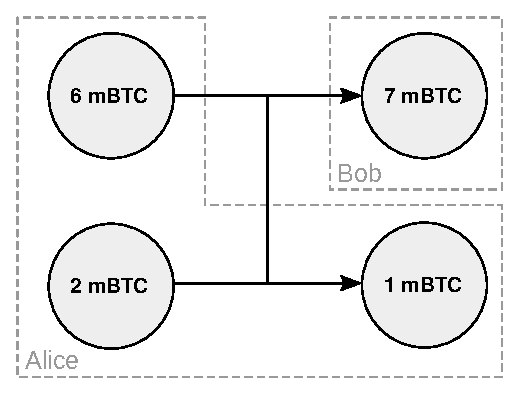
\includegraphics[scale=0.75]{img/transaction-2i-2o.eps}
  \caption{Schéma d'une transaction à 2 entrées et 2 sorties.}
  \label{fig:transaction-2i-2o}
\end{figure}

% Transaction à 3 entrées et 1 sortie
Si Alice désire transférer l'intégralité des fonds vers un autre compte, alors elle rassemble l'ensemble de ses pièces (6~mBTC, 4~mBTC, 2~mBTC) pour les envoyer vers une adresse unique, comme montré sur la figure~\ref{fig:transaction-3i-1o}). C'est ce qu'on appelle une consolidation de portefeuille, qui peut être identifiée par un observateur extérieur en raison de l'unicité de la sortie.

\begin{figure}[ht]
  \centering
  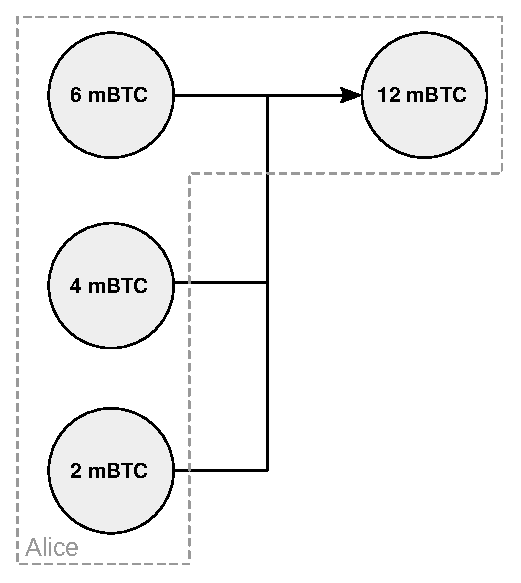
\includegraphics[scale=0.75]{img/transaction-3i-1o.eps}
  \caption{Schéma d'une transaction à 2 entrées et 1 sortie.}
  \label{fig:transaction-3i-1o}
\end{figure}

% Conclusion sur le modèle de représentation par des pièces
Nous voyons ainsi que les transactions ne sont pas des transferts bruts d'une adresse vers une autre, mais des combinaisons ou des séparations de pièces de monnaies numériques. Ce fonctionnement est quelque peu contre-intuitif, mais se révèle utile pour la scalabilité du système, en permettant le traitement indépendant des pièces, et pour la confidentialité des utilisateurs, en n'incitant pas au rassemblement sur une même adresse et en facilitant l'implémentation de techniques d'anonymisation comme le mélange des pièces. Ce modèle est donc particulièrement adapté à l'utilisation monétaire\sendnote{Ludovic Lars, \emph{Pièces et comptes~: deux modèles de représentation}, 20 juillet 2019~: \url{https://viresinnumeris.fr/pieces-comptes-modeles-representation/}.}.

% % Exemple de Satoshi Nakamoto et de Hal Finney
% L'identifiant de la première transaction réalisée entre Satoshi Nakamoto et Hal Finney était~:
%
% \begin{verbatim}
% f4184fc596403b9d638783cf57adfe4c75c605f6356fbc91338530e9831e9e16
% \end{verbatim}
%
% Satoshi Nakamoto utilisait une pièce de 50~BTC, minée précédemment, pour créer une pièce de 10~BTC à l'adresse de Hal. Il se rendait la monnaie à la même adresse.

\section*{La machine virtuelle}
\addcontentsline{toc}{section}{La machine virtuelle}

% Monnaie programmable
Les scripts présents au sein des transactions font de Bitcoin un système de monnaie programmable. Ces scripts permettent en effet la mise en place d'une variété de conditions de dépense, aussi appelées clauses, qui vont au-delà de l'exigence d'une signature simple, comme la connaissance d'un secret, l'attente d'une période de temps ou la production de signatures multiples.

% Machine abstraite répliquée, machine virtuelle, machine à états
La mise en œuvre de Bitcoin crée une machine abstraite dont le fonctionnement est répliqué sur tous les nœuds du réseau grâce à l'algorithme de consensus. Elle est simulée par l'intermédiaire de l'implémentation logicielle, de sorte qu'on parle de machine virtuelle. Plus précisément, il s'agit d'un machine à états, dont l'état courant est l'ensemble des pièces existantes, c'est-à-dire l'ensemble des sorties transactionnelles non dépensées (UTXO), et dont les transitions sont les transactions, qui détruisent des pièces pour en créer de nouvelles. Ces transactions sont assemblées dans des blocs qui sont validés à intervalles réguliers par les mineurs. La diffusion d'un bloc sur le réseau permet d'actualiser l'état de la machine virtuelle, qui est la plupart du temps partagé par tous les nœuds.

% réplication de machine à états (\eng{state machine replication})
% FAUX : automate fini (appelé \eng{finite-state machine} en anglais) qui peut être dans une quantité finie d'états, mais qui n'est, à un moment donné, que dans un seul état\sendnote{Contrairement à ce qui est parfois affirmé, la machine virtuelle n'est pas un automate à deux piles (\eng{dual-stack pushdown automaton}), même si le langage de programmation interne en émule un. -- Craig S. Wright, \eng{Beyond Godel}, 2018~: \url{https://coingeek.com/wp-content/uploads/2018/03/SSRN-id3147440.pdf}.}. Même s'il est très grand, l'ensemble des états possibles est nécessairement fini en raison du codage des entiers sur 8 octets et de la limite de taille des scripts\sendnote{La limite de taille des scripts est actuellement de 10~ko sur BTC~: \url{https://github.com/bitcoin/bitcoin/blob/v0.17.0/src/script/script.h\#L31-L32}.}.

% Exécution des scripts
Au sein d'une transaction, le déverrouillage des pièces se fait par l'exécution de scripts. Les scripts sont des prédicats au sens mathématique, c'est-à-dire des expressions incomplètes qui deviennent des propositions pouvant être évaluées si elles sont complétées par un ou plusieurs éléments. De ce fait, la dépense consiste à réunir le script de verrouillage de la sortie précédente et le script de déverrouillage, et à les exécuter l'un après l'autre~: le script de déverrouillage d'abord, le script de verrouillage ensuite. L'utilisation de la pièce comme entrée de transaction n'est approuvée que si l'exécution réussit.

% Langage de programmation (règles de transition)
Les scripts sont écrits dans le langage de programmation interne de Bitcoin, conçu par Satoshi Nakamoto dès 2008 et baptisé de façon peu originale «~Script~». Ce langage de programmation fonctionne de manière similaire à Forth, un langage utilisé dans les années 1970 et 1980. Il se base en particulier sur deux piles de données, qui sont des structures de données fondées sur le principe du «~dernier arrivé, premier sorti~» (de l'anglais \eng{last in, first out}, abrégé en LIFO). Le langage agit essentiellement sur la pile primaire, de sorte que cette dernière est la plus importante~; la pile secondaire permet seulement de mettre des données de côté pendant l'exécution d'un script.

% Description par Satoshi
Satoshi Nakamoto a inclus ce système de scripts dans Bitcoin pour lui permettre de gérer une grande variété de cas d'utilisation. En juin 2010, en réponse à Gavin Andresen, il écrivait ainsi sur le forum~:

\begin{quote}
«~La nature de Bitcoin est telle que, dès la version 0.1 lancée, son fonctionnement de base était gravé dans le marbre pour le reste de son existence. C'est pour cette raison que je voulais concevoir Bitcoin pour qu'il supporte tous les types de transaction auxquels je pouvais penser. Le problème était que chaque élément requérait un code de prise en charge et des champs de données spéciaux, qu'il soit utilisé ou non, et ne pouvait couvrir qu'un cas particulier à la fois. Ç'aurait été une explosion de cas particuliers. La solution était script, qui généralisait le problème de façon à ce que les parties contractantes puissent décrire leurs transactions comme des prédicats que les nœuds du réseau évaluaient. Les nœuds ont seulement besoin de comprendre la transaction dans la mesure où ils évaluent si les conditions de l'émetteur sont remplies ou non.\sendnote{Satoshi Nakamoto, \eng{Re: Transactions and Scripts: DUP HASH160 ... EQUALVERIFY CHECKSIG}, \wtime{17/06/2010 18:46:08}~: \url{https://bitcointalk.org/index.php?topic=195.msg1611\#msg1611}.}~»
\end{quote} % "The nature of Bitcoin is such that once version 0.1 was released, the core design was set in stone for the rest of its lifetime.  Because of that, I wanted to design it to support every possible transaction type I could think of.  The problem was, each thing required special support code and data fields whether it was used or not, and only covered one special case at a time.  It would have been an explosion of special cases.  The solution was script, which generalizes the problem so transacting parties can describe their transaction as a predicate that the node network evaluates.  The nodes only need to understand the transaction to the extent of evaluating whether the sender's conditions are met."

% Opérateurs
Le langage est constitué de plus d'une centaine d'opérateurs, aussi appelés codes opération (ou \eng{opcodes} en anglais), qui agissent sur la pile primaire d'une manière ou d'une autre\sendnote{La liste des opérateurs et de leurs actions est disponible sur la page de Bitcoin Wiki consacrée à Script~: \url{https://en.bitcoin.it/wiki/Script}.}. Les opérateurs sont des nombres codés sur 1 octet (allant de 0 à 255), mais sont usuellement désignés par un nom décrivant leur fonction, dans le but de rendre la lecture plus compréhensible par l'être humain. Ils sont notés en majuscules et sont souvent précédés du préfixe \texttt{OP\_} même s'il peut être omis en l'absence d'ambiguïté. Par exemple, l'opérateur permettant de vérifier une signature (\texttt{0xac}) est noté \texttt{OP\_CHECKSIG} ou \texttt{CHECKSIG}.

% Empilement
Les opérateurs allant de 1 à 75, parfois notés \texttt{OP\_PUSHBYTES\_X}, ont pour action d'empiler des données ayant une taille allant de 1 à 75 octets. L'utilisation d'opérateurs supplémentaires spécifiques (notés \texttt{OP\_PUSHDATA\_Y}) permet cependant de placer une information plus grande sur la pile. Bien qu'on puisse utiliser cette notation, il est généralement plus simple de placer un élément entre chevrons pour indiquer qu'il est placé au sommet de la pile. Par exemple, le fait d'écrire \texttt{<signature>} au sein d'un script signifie que la signature est empilée.

% Valeur retournée
La valeur retournée à la fin de l'exécution des scripts est un booléen, de sorte que le script peut être valide, auquel cas la dépense de la pièce est approuvée, ou bien invalide, auquel cas la transaction est rejetée dans son ensemble. Le script est valide si et seulement si la valeur \texttt{TRUE} («~vrai~» en anglais) est présente en haut de la pile à la fin de l'exécution. Il est invalide si ce n'est pas le cas ou si son exécution s'est arrêtée avant la fin.

% Pas de boucles
Le langage Script est cependant limité. Rien dans sa conception ne permet pas de faire de boucles, ni d'accéder à des données extérieures à celles de la transaction, contrairement au langage d'Ethereum qui est quasi Turing-complet. Cette particularité fait qu'il est moins flexible, mais qu'il a l'avantage d'être plus simple à appréhender et donc plus sûr.

% Exemple : vérification d'une addition (38 = 17 + x)
L'exemple typique de script, présenté par Andreas Antonopoulos\sendnote{Andreas Antonopoulos, \eng{Mastering Bitcoin (second edition)}, ch.6, 2017.}, est celui qui consiste à résoudre une équation simple impliquant une addition. Si on considère l'équation $17 + x = 38$, alors le script de verrouillage qui correspond est~:

\begin{Verbatim}[fontsize=\footnotesize]
<17> ADD <38> EQUAL
\end{Verbatim}

Toute personne disposant de la réponse peut dépenser la pièce, ce qui on en convient n'est pas très sécurisé. La dépense requiert ici de fournir le script de déverrouillage composé uniquement de la solution de l'équation, à savoir 21~:

\begin{Verbatim}[fontsize=\footnotesize]
<21>
\end{Verbatim}

L'exécution successive de ces deux scripts (voir figure~\ref{fig:bitcoin-stack}) a lieu comme suit~: 1)~la valeur 21 est placée sur la pile~; 2)~la valeur 17 est placée au-dessus~; 3)~l'opérateur \texttt{OP\_ADD} additionne les deux valeurs en haut de la pile et les remplace par leur somme, ici 38~; 4)~la valeur 38 est placée au sommet de la pile~; 5)~l'opérateur \texttt{OP\_EQUAL} compare les deux valeurs en haut de la pile et les remplace par le booléen d'égalité, ici \texttt{TRUE}. L'exécution du script est donc un succès.

\begin{figure}[ht]
  \centering
  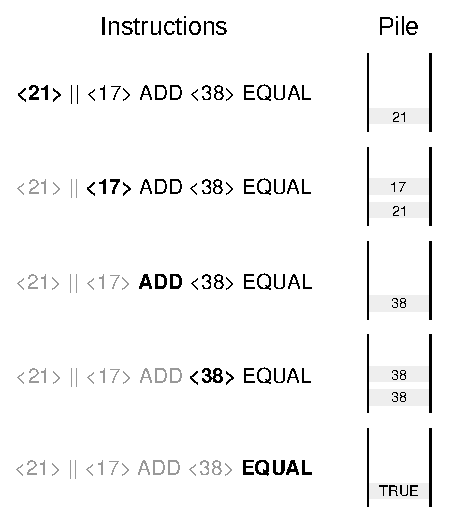
\includegraphics[scale=0.75]{img/bitcoin-stack-example.eps}
  \caption{Exécution d'un script d'addition sur la pile de données.}
  \label{fig:bitcoin-stack}
\end{figure}

Si la valeur avait été différente, 22 par exemple, alors la dernière opération aurait retourné le booléen \texttt{FALSE} et la transaction de dépense aurait été invalidée.

% --- Exemples de scripts complets ---

Beaucoup de conditions de dépense différentes peuvent être implémentées par ce système. Certaines de ces conditions sont simples comme la connaissance d'un secret spécifique ou la production d'une signature valide correspondant à une clé publique particulière.

La connaissance d'un secret (dont l'empreinte est spécifiée dans l'UTXO) est vérifiée par les scripts suivants qui placent le secret au sommet de la pile, le hachent par SHA-256 et comparent le résultat à l'empreinte~:

\begin{Verbatim}[fontsize=\footnotesize]
<secret> || SHA256 <empreinte> EQUAL
\end{Verbatim}

De même, la vérification de la validité d'une signature est réalisée par les scripts suivants qui empilent d'abord la signature, puis la clé publique avant de contrôler leur correspondance~:

\begin{Verbatim}[fontsize=\footnotesize]
<signature> || <clé publique> CHECKSIG
\end{Verbatim}

% Verrous temporels
Mais il existe des conditions plus avancées comme les verrous temporels. Ceux-ci permettent de bloquer les fonds de la pièce pour un temps précis, que ce soit jusqu'à une date donnée, auquel cas on parle de temps de verrouillage absolu, ou bien pendant une période donnée, auquel cas on parle de temps de verrouillage relatif. Le premier est le fait de l'opérateur \texttt{OP\_CHECKLOCKTIMEVERIFY} dont les spécificités techniques sont décrites dans le BIP-65. Le second est appliqué par le code opération \texttt{OP\_CHECKSEQUENCEVERIFY} décrit dans le BIP-112.

% DESCRIPTION TECHNIQUE
%
% Les scripts suivants vérifient un temps de verrouillage absolu, c'est-à-dire lié à une date particulière~:
%
% \begin{verbatim}
% TRUE || <date de verrouillage> CHECKLOCKTIMEVERIFY DROP
% \end{verbatim}
%
% Le booléen \verb?TRUE? est mise en haut de la pile. Puis, est empilée la date jusqu'à laquelle le verrouillage persiste, qui est donnée en horodatage MTP ou en hauteur de blocs. Ensuite, cette date est comparée à la date indiquée dans le champ \verb?nLocktime? de la transaction, qui est elle-même comparée à l'horodatage du réseau. Enfin, la date est expulsée de la pile, ce qui fait qu'il ne reste que le booléen \verb?TRUE? sur la pile.
%
% Les scripts suivants vérifient un verrou temporel relatif, qui est lié à la période de temps écoulée depuis la date de confirmation de la pièce~:
%
% \begin{verbatim}
% TRUE || <période de verrouillage> CHECKSEQUENCEVERIFY DROP
% \end{verbatim}
%
% Le booléen \verb?TRUE? est mise en haut de la pile. Puis, c'est au tour de la période de verrouillage, qui est donnée en secondes\sendnote{Ou plus précisément en unités de 512 secondes.} ou en nombre de blocs. Ensuite, cette période est comparée à la période de temps indiquée dans le champ \verb?nSequence? de l'entrée dépensant la pièce, qui est elle-même comparée à la période de temps écoulée depuis la date de confirmation de la pièce. Enfin, la période est expulsée de la pile, ne laissant que le booléen \verb?TRUE? au sommet de la pile.
%
% Ce fonctionnement un peu plus compliqué des verrous temporels s'explique par le fait qu'ils ont été intégrés sous la forme de soft fork.


\section*{Les schémas classiques}
\addcontentsline{toc}{section}{Les schémas classiques}

% --- Schémas et règles de mempool ---

Le langage Script permet de faire des choses diverses et variées. Pendant les premiers temps de Bitcoin, le système était relativement libre et autorisait les gens à écrire ce qu'ils voulaient dans les scripts sans discrimination. Toutefois, cette situation était considérablement risquée. La raison principale était que le fonctionnement des codes opération n'était pas encore vérifié et testé, comme l'a montré la découverte en juillet 2010 d'une vulnérabilité rendue possible par certains opérateurs binaires\sendnote{NIST, \eng{CVE-2010-5137}, 8 juin 2012~: \url{https://nvd.nist.gov/vuln/detail/CVE-2010-5137}.}. C'est pourquoi il a été décidé à la fin de l'année 2010, sous l'impulsion de Gavin Andresen, de restreindre la facilité de programmation du système\sendnote{Gavin Andresen, \eng{svn r197: IsStandard check for transactions}, \wtime{07/12/2010 13:58:33 UTC}~: \url{https://bitcointalk.org/index.php?topic=2129.msg27744\#msg27744}.}.

% Schémas standards
Cette restriction a été appliquée en imposant des schémas standards de scripts, qui faisaient que les nœuds configurés par défaut ne relayaient plus les transactions contenant des scripts qui ne respectaient pas ce standard. Il ne s'agissait pas ainsi d'une restriction des règles globales de consensus, mais des règles locales de mempool qui s'applique à la transmission des transactions. Des schémas standards rendant les choses plus simples et plus sûres ont ainsi été développés au cours des années. Les schémas standards de sortie transactionnelle étaient \textcolor{darkgray}{en 2023} au nombre de huit~: P2PK, P2PKH, P2MS, P2SH, NULLDATA, P2WPKH, P2WSH et P2TR\sendnote{\url{https://github.com/bitcoin/bitcoin/blob/22.x/src/script/standard.h\#L59-L71}.}.

% --- Pay to Public Key ---

\textbf{P2PK~: Pay to Public Key} Le premier schéma s'appelle Pay to Public Key (P2PK), qu'on peut traduire littéralement en français par «~payer à la clé publique~». Il s'agit de créer une pièce liée à la clé publique d'un destinataire, que lui seul peut dépenser en signant avec sa clé privée. Le script de verrouillage permettant ce type d'envoi est~:

\begin{Verbatim}[fontsize=\footnotesize]
<clé publique> CHECKSIG
\end{Verbatim}

La présence de la clé publique explique qu'on parle parfois de «~scriptPubKey~» pour désigner le script de verrouillage en général, indépendemment de ce qu'il contient.

Au moment de la dépense, le destinataire doit utiliser un script de déverrouillage contenant simplement sa signature~:

\begin{Verbatim}[fontsize=\footnotesize]
<signature>
\end{Verbatim}

La présence de la signature dans ce script explique qu'on parle parfois de «~scriptSig~» pour désigner le script de déverrouillage en général, indépendemment de ce qu'il contient.

L'exécution successive de ces deux scripts permet, comme on l'a vu, de vérifier que la signature fournie par l'utilisateur correspond à sa clé publique, auquel cas elle est valide.

Le schéma P2PK était utilisé dans les débuts de Bitcoin pour recevoir les paiements par IP (P2IP) et pour récupérer la récompense de minage. Il est aujourd'hui tombé en désuétude au profit d'un schéma rival~: P2PKH.

% --- Pay to Public Key Hash --

\textbf{P2PKH~: Pay to Public Key Hash.} Le schéma Pay to Public Key Hash (P2PKH), qui est traduit littéralement par «~payer à l'empreinte de la clé publique~», est le deuxième type de format de réception apparu dans Bitcoin dès le début du fait de la conception de Satoshi Nakamoto. Ce schéma permet non pas de réaliser un paiement vers une clé publique, mais vers l'empreinte d'une clé publique, tout en faisant en sorte que l'interpréteur vérifie quand même la validité de la signature vis-à-vis de la clé publique lors de la dépense des fonds. L'empreinte de la clé publique est alors considérée comme la donnée essentielle de l'adresse, qui dans ce cas commence toujours par un 1, comme par exemple \longstring{1FjBKPQ7MTiPSDkJ2ZwPgAXUKQ8yoGbVJX}.

Le script de verrouillage ici est~:

\begin{Verbatim}[fontsize=\footnotesize]
DUP HASH160 <empreinte de la clé publique> EQUALVERIFY CHECKSIG
\end{Verbatim}

Et le script de déverrouillage est~:

\begin{Verbatim}[fontsize=\footnotesize]
<signature> <clé publique>
\end{Verbatim}

L'exécution des deux scripts permet de~: 1) vérifier que le passage de la clé publique par la fonction de hachage HASH-160 est égale à l'empreinte qui est spécifiée dans le script ; 2) vérifier la signature correspond à la clé publique.

L'avantage de ce schéma est qu'il permet d'avoir des adresses plus courtes (l'information à encoder n'est que de 20~octets au lieu de 65~octets pour une clé publique), raison pour laquelle Satoshi Nakamoto l'a implémenté. De plus, en ne révélant la clé publique qu'au moment de la dépense, ce schéma accroît aussi la sécurité contre la menace (très hypothétique) de l'ordinateur quantique.

% --- Pay To MultiSig ---

\textbf{P2MS~: Pay To MultiSig.} Le schéma Pay To MultiSig (P2SH), qui signifie littéralement «~payer à la multisignature~», est un schéma exigeant la signature de M personnes parmi N participants prédéterminés («~M-parmi-N~», ou «~M-of-N~» en anglais). Il a été rendu standard sous une forme limitée à 3 participants en mars 2012 avec la sortie de la version 0.6.0 du logiciel\sendnote{Gavin Andresen, \eng{Version 0.6.0 released}, 30 mars 2012~: \url{https://bitcointalk.org/index.php?topic=74737.msg827484\#msg827484}.}. Le script de verrouillage est le suivant~:

\begin{Verbatim}[fontsize=\footnotesize]
M <clé publique 1> ... <clé publique N> N CHECKMULTISIG
\end{Verbatim}

Le script de déverrouillage correspondant est~:

\begin{Verbatim}[fontsize=\footnotesize]
<leurre (0)> <signature 1> ... <signature M>
\end{Verbatim}

La présence du leurre (généralement 0) est dû à un défaut dans l'implémentation de l'exécution de l'opérateur \texttt{OP\_CHECKMULTISIG} par Satoshi, qui requiert un élément de trop. Les développeurs n'ont pas jugé rentable de corriger ce défaut, car cette correction constituait un hard fork.

C'est ce schéma, particulièrement exigeant au niveau de la mise en place, qui a motivé la création du schéma P2SH.

\textbf{P2SH : Pay to Script Hash} Le schéma Pay to Script Hash (P2SH), pouvant être traduit littéralement par «~payer à l'empreinte du script~», reprend l'idée derrière P2PKH, à la seule différence que la donnée hachée n'est pas une clé publique, mais le script lui-même~! Le script en question est alors appelé script de récupération (\eng{redeem script}) pour le différencier du script de déverrouillage. Son empreinte est la donnée constituante de l'adresse, cette dernière commençant toujours par un 3 à l'instar de \longstring{3K8Ps6Ayw5ZaKDaLZjfGo3mTgDsc1VXZ8d}.

% \sendnote{Ludovic Lars, \emph{Pay to Script Hash (P2SH) pleinement expliqué}, 14 juillet 2020~: \url{https://viresinnumeris.fr/pay-to-script-hash-p2sh-pleinement-explique/}.}

Ce schéma donne à l'utilisateur la possibilité d'y inclure n'importe quel script, sans discrimination sur son format, à condition qu'il respecte bien sûr certaines limites. Il permet aussi de recevoir des fonds depuis la quasi-totalité des portefeuilles existants, le fardeau de la construction et du déverrouillage du script revenant uniquement au destinataire, et pas aussi à l'expéditeur comme c'est le cas dans le scripting brut.

Le script de verrouillage pour le schéma P2SH est~:

\begin{Verbatim}[fontsize=\footnotesize]
HASH160 <empreinte du script de récupération> EQUAL
\end{Verbatim}

Et le script de déverrouillage est un script de la forme~:

\begin{Verbatim}[fontsize=\footnotesize]
[éléments de déverrouillage] <script de récupération>
\end{Verbatim}

L'exécution de P2SH est plus complexe que les précédents schémas, ce qui peut s'expliquer par le contexte dans lequel il a été développé. L'idée d'implémenter un schéma de script qui utilise l'empreinte d'un autre script comme l'empreinte de clé publique dans le schéma P2PKH est née 2011 en faisant l'objet de plusieurs propositions\sendnote{Mike Caldwell (casascius), \eng{Proposal to modify OP\_CHECKSIG}, \wtime{22/09/2011 02:21:17 UTC}~: \url{https://bitcointalk.org/index.php?topic=45211.msg538756\#msg538756}~; jimrandomh, \eng{Proposed extensions to the transaction protocol: Receiver scripts, OP\_TIME, more}, \wtime{01/10/2011 16:56:47 UTC}~: \url{https://bitcointalk.org/index.php?topic=46429.msg553217\#msg553217}~; Gavin Andresen, \eng{Re: Proposal to modify OP\_CHECKSIG}, \wtime{02/10/2011 00:26:42 UTC}~: \url{https://bitcointalk.org/index.php?topic=45211.msg553668\#msg553668}.}. Elle a été rendue plus concrète avec une proposition de l'opérateur \texttt{OP\_EVAL} par Nicolas van Saberhagen le 2 octobre, code opération qui permettait l'exécution récursive d'un script à l'intérieur d'un autre script\sendnote{Nicolas van Saberhagen (ByteCoin), \eng{OP\_EVAL proposal}, \wtime{02/10/2011 00:49:19 UTC}~: \url{https://bitcointalk.org/index.php?topic=46538.msg553689\#msg553689}.}. Gavin Andresen a expliqué comment en faire un soft fork par le remplacement de l'instruction sans effet \texttt{OP\_NOP1}\sendnote{Gavin Andresen, \eng{Re: OP\_EVAL proposal}, \wtime{02/10/2011 20:42:32 UTC}~: \url{https://bitcointalk.org/index.php?topic=46538.msg554620\#msg554620}.}.

L'opérateur \texttt{OP\_EVAL} devait permettre de former un nouveau schéma standard. Le script de verrouillage aurait été~:

\begin{Verbatim}[fontsize=\footnotesize]
DUP HASH160 <empreinte du script de récupération> EQUALVERIFY EVAL
\end{Verbatim}

tandis que le script de déverrouillage aurait été le même. L'exécution successive de ces deux scripts aurait permis dans un premier temps de vérifier la conformité du hachage du script de récupération à l'empreinte~; puis dans un second temps d'exécuter le script de récupération et de lui combiner les éléments de déverrouillage.

Néanmoins cette solution n'a pas été acceptée, celle-ci ayant été jugée trop dangereuse à cause de son pouvoir de récursion. Il lui a été préféré le modèle plus restrictif de P2SH.

L'exécution de P2SH fonctionne exactement comme le schéma lié à \texttt{OP\_EVAL}, à l'exception qu'une partie du script n'est pas explicitement indiquée. D'une part, la vérification de la correspondance entre l'empreinte indiquée et le script de récupération est bien réalisée par le script de verrouillage. D'autre part, l'évaluation du script de récupération est effectuée implicitement grâce à une exception ajoutée au code source qui fait que les nœuds du réseau qui reconnaissent le schéma l'interprètent différemment. Dans Bitcoin Core, on peut observer cette condition au sein de la fonction \texttt{VerifyScript} de l'interpréteur\sendnote{\url{https://github.com/bitcoin/bitcoin/blob/22.x/src/script/interpreter.cpp\#L2018-L2062}}.

% Laideur
La proposition a été codifiée dans le BIP-16. Si cette solution est pratique, elle crée de la complexité et n'est pas très élégante. Comme le disait Gavin Andresen dans l'explication du BIP-16~:

\begin{quote}
«~Reconnaître une forme "spéciale" de scriptPubKey et réaliser une validation supplémentaire quand elle est détectée, c'est laid. Cependant, l'avis général est que les alternatives sont soit encore plus laides, soit plus complexes à implémenter, et/ou étendent le pouvoir du langage d'expression de manière dangereuse.\sendnote{Gavin Andresen, \eng{BIP-16: Pay to Script Hash}, 3 janvier 2012~: \url{https://github.com/bitcoin/bips/blob/master/bip-0016.mediawiki\#rationale}.}~»
\end{quote}

Le schéma P2SH a été activé le 1\ier{} avril 2012 sous la forme d'un soft fork, en dépit de l'opposition notable de luke-jr qui proposait un opérateur alternatif, \texttt{OP\_CHECKHASHVERIFY}, décrit dans le BIP-17\sendnote{Amir Taaki, \eng{The Truth behind BIP 16 and 17}, 29 janvier 2012~: \url{http://bitcoinmedia.com/the-truth-behind-bip-16-and-17/}~; archive~: \url{https://web.archive.org/web/20120202032835/http://bitcoinmedia.com/the-truth-behind-bip-16-and-17/}.}.

\textbf{NULLDATA} Le schéma, signifiant littéralement «~données insignifiantes~», est un schéma d'inscription de données arbitraires sur la chaîne. Il est le quatrième schéma classique et a été rendu standard avec l'arrivée de la version 0.9.0 de Bitcoin Core en mars 2014\sendnote{\eng{Bitcoin Core version 0.9.0 released}, 19 mars 2014~: \url{https://bitcoin.org/en/release/v0.9.0\#opreturn-and-data-in-the-block-chain}.}. Il se base sur l'instruction \texttt{OP\_RETURN} dont l'effet est de mettre fin à l'exécution du script et de rendre indépensable la pièce correspondante\sendnote{L'instruction \texttt{OP\_RETURN} servait initialement à retourner la valeur au sommet de la pile, d'où son nom. Cependant, en juillet 2010, la découverte du «~\eng{1 RETURN bug}~», qui permettait de dépenser toute sortie transactionnelle via le script de déverrouillage \texttt{TRUE RETURN}, a poussé Satoshi Nakamoto à désactiver cette fonctionnalité en lui faisant renvoyer \texttt{FALSE} systématiquement (\url{https://github.com/bitcoin/bitcoin/commit/a75560d828464c3f1138f52cf247e956fc8f937d}).}. Le script de verrouillage du schéma commence toujours par \texttt{OP\_RETURN} et est suivi des données empilées~:

\begin{Verbatim}[fontsize=\footnotesize]
RETURN [données arbitraires]
\end{Verbatim}

La sortie contenant ce script est exempt de la limite standarde de poussière, qui est \textcolor{darkgray}{actuellement de 546 satoshis pour les sorties P2PKH}, de sorte qu'elle peut être de 0 satoshis. La taille maximale des données pouvant être inscrite est de \textcolor{darkgray}{80~octets par transaction} sur BTC. De plus, en raison de leur caractère assurément indépensable, les sorties peuvent être retranchées de l'ensemble des UTXO des nœuds. Tout ceci fait de ce schéma le moyen normal d'inscrire des informations sur le registre.

\section*{Les types de signature}
\addcontentsline{toc}{section}{Les types de signature}

% --- Types de signature ---

La programmabilité de Bitcoin n'est pas seulement issue de son langage de programmation mais aussi du système de signature qui permet de de sélectionner quelle partie de la transaction est signée. Ce facteur de programmabilité est mis en œuvre par l'existence d'un indicateur, appelé type de hachage de la signature ou \eng{signature hash type}, qui est ajouté à la transaction non signée, puis à la signature elle-même. Celui-ci indique quelle partie de la transaction doit être hachée avant d'être soumise à l'algorithme de signature, d'où son nom.

Le type de signature est construit à partir de plusieurs signaux de signature qui peuvent être combinés. Les quatre signaux de signature qui existent sont~:

\begin{itemize}
\item[$\bullet$] \texttt{SIGHASH\_ALL} (\texttt{0x01}) qui indique que toutes les sorties sont signées~;
\item[$\bullet$] \texttt{SIGHASH\_SINGLE} (\texttt{0x03}) qui permet de ne signer qu'une seule sortie~;
\item[$\bullet$] \texttt{SIGHASH\_NONE} (\texttt{0x02}) qui indique qu'aucune sortie n'est signée~;
\item[$\bullet$] \texttt{SIGHASH\_ANYONECANPAY} (\texttt{0x80}) qui permet de ne signer qu'une seule entrée.
\end{itemize}

Les trois signaux concernant les sorties peuvent être associés à \longstring{SIGHASH\_ANYONECANPAY}, ce qui permet de former finalement six types de signature différents, représentés sur la figure~\ref{fig:signature-hash-types}. Le type de signature le plus fréquent est évidemment \longstring{SIGHASH\_ALL} même si certains autres types peuvent parfois trouver une utilité. C'est notamment le cas de \longstring{SIGHASH\_ALL | SIGHASH\_ANYONECANPAY} qui permet de construire des transactions de type \eng{anyone-can-pay}, dont les sorties sont déterminées, mais où chacun peut signer sa propre entrée sans connaître les autres.

\begin{figure}[ht]
  \centering
  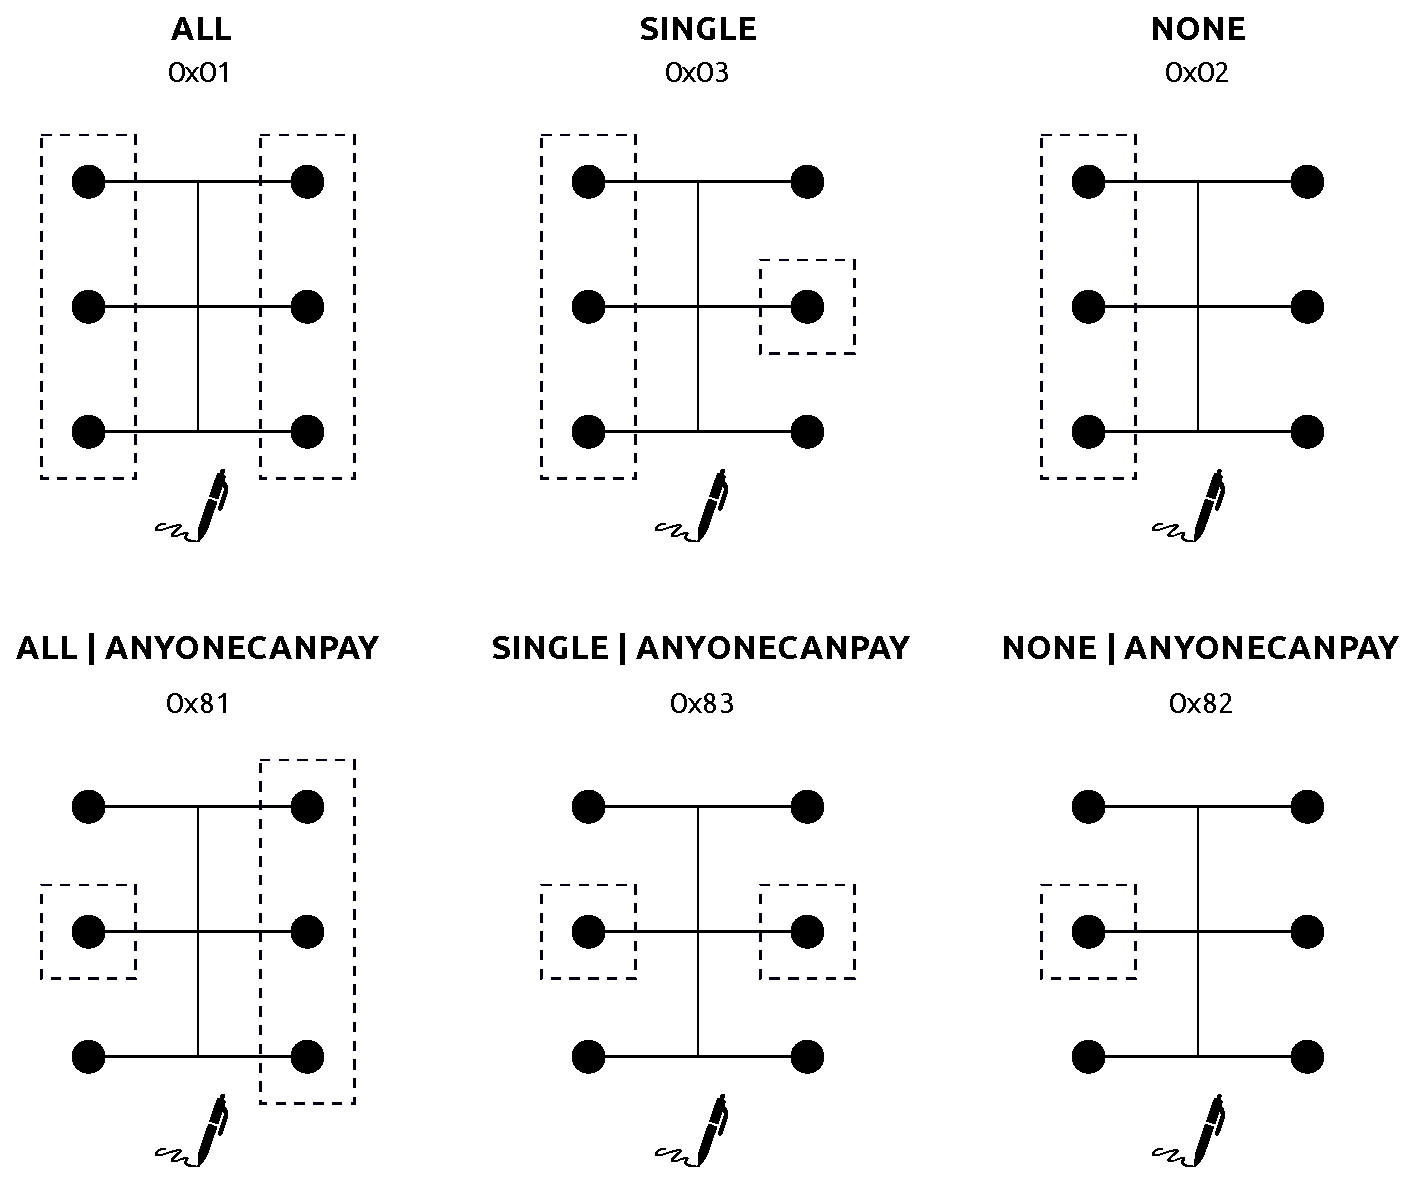
\includegraphics[scale=0.45]{img/signature-hash-types.eps}
  \caption{Les différents types de signature dans Bitcoin.}
  \label{fig:signature-hash-types}
\end{figure}

% Notez que tout ceci était présent dès la création de Bitcoin et que Satoshi Nakamoto avait intégré ce type de signature dans le code d'origine.

% SIGHASH_NOINPUT
Ces signaux ont été implémentés dès le début par Satoshi Nakamoto au sein du prototype. Il en manquait logiquement un, que Satoshi Nakamoto a probablement jugé inutile~: celui qui ne signait aucune entrée. Toutefois, avec le développement des canaux de paiements pour le réseau Lightning, les développeurs se sont rendus compte qu'il pouvait avoir une utilité. C'est dans cet esprit que le signal de signature \longstring{SIGHASH\_NOINPUT} a été proposé en février 2016 par Joseph Poon\sendnote{Joseph Poon, \eng{[bitcoin-dev] SIGHASH\_NOINPUT in Segregated Witness}, \wtime{26/02/2016 01:07:46 UTC}~: \url{https://lists.linuxfoundation.org/pipermail/bitcoin-dev/2016-February/012460.html}.}.

% BIP-118, SIGHASH_ANYPREVOUT
Ce type de signal pourrait être implémenté de manière partielle dans BTC au travers du BIP-118, qui prévoit l'implémentation de deux nouveaux signaux -- \longstring{SIGHASH\_ANYPREVOUT} et \longstring{SIGHASH\_ANYPREVOUTANYSCRIPT} -- au sein des scripts de Taproot\sendnote{Christian Decker, Anthony Towns, \eng{BIP-118: SIGHASH\_ANYPREVOUT for Taproot Scripts}, 28 février 2017~: \url{https://github.com/bitcoin/bips/blob/master/bip-0118.mediawiki}.}. Il permettrait d'améliorer le fonctionnement du réseau Lightning par la mise en œuvre du protocole Eltoo qui repose sur la construction de transactions flottantes.

\section*{SegWit~: le témoin séparé}
\addcontentsline{toc}{section}{SegWit~: le témoin séparé}

% Présentation de SegWit
SegWit, abréviation de \eng{Segregated Witness}, qu'on peut traduire littéralement par «~témoin séparé~», est une mise à niveau du protocole ayant lieu sur LTC et sur BTC en 2017. Elle a consisté à faire en sorte que les données de déverrouillage des entrées transactionnelles, telles que les signatures, se retrouvent dans une structure de données séparée (\eng{segregated}) appelée le témoin (\eng{witness}) afin de supprimer la malléabilité des transactions. SegWit constituait ainsi une restructuration profonde des transactions.

% Autres apports
Outre la correction de la malléabilité, SegWit a apporté une augmentation de capacité transactionnelle et un versionnage des scripts pour faciliter les mises à niveau ultérieures. Elle a également amélioré l'algorithme de signature pour éviter les hachages redondants durant la vérification et pour rendre plus sûre la signature hors-ligne\sendnote{Voir BIP-143~: \url{https://github.com/bitcoin/bips/blob/master/bip-0143.mediawiki}.}.

% --- Malléabilité ---

\textbf{Malléabilité.} SegWit tire son origine du problème de la malléabilité des transactions, un problème identifié depuis janvier 2012\sendnote{Gavin Andresen, \eng{[Bitcoin-development] Extending IsStandard() to transaction scriptSigs}, \wtime{19/1/2012 16:29:29}, \url{https://lists.linuxfoundation.org/pipermail/bitcoin-dev/2012-January/001066.html}.}. Dans Bitcoin, les transactions sont malléables dans le sens où elles peuvent être modifiées légèrement après leur diffusion sans devenir invalides aux yeux du réseau. Cette propriété vient du fait qu'une signature ne peut pas se prendre en compte elle-même et que par conséquent le script de déverrouillage n'est pas signé avec le reste de la transaction. La malléabilité peut ainsi prendre deux formes~: la malléabilité intrinsèque à l'algorithme ECDSA, qui se base sur un nombre aléatoire pour produire une signature (malléabilité par le signataire)~; la malléabilité provenant de la forme des signatures et des scripts de déverrouillage des entrées (malléabilité par un tiers).

% Problèmes
La malléabilité n'est pas rédhibitoire pour la sécurité des fonds, mais elle permet de modifier l'identifiant de la transaction après sa publication, ce qui peut se révéler problématique dans certaines situations. Ainsi, entre le 9 et le 11 février 2014, Mt. Gox et d'autres plateformes d'échange ont subi des attaques exploitant cette malléabilité des transactions\sendnote{Ken Shirriff, \eng{The Bitcoin malleability attack graphed hour by hour}, 15 février 2014~: \url{https://www.righto.com/2014/02/the-bitcoin-malleability-attack-hour-by.html}}. Les transactions de retrait ont été modifiées par les attaquants, faisant croire aux plateformes mal configurées que ces transactions n'avaient pas été confirmées, ce qui leur a permis de recréditer leur compte tout en conservant les bitcoins. Ces attaques ont mené à une perte totale de 64~564~bitcoins\sendnote{Christian Decker, Roger Wattenhofer, \eng{Bitcoin Transaction Malleability and MtGox}, 26 mars 2014~: \url{https://arxiv.org/pdf/1403.6676.pdf\#page=8}.}.

% Tentatives de correction
Des propositions ont tenté de corriger la malléabilité par un tiers en contraignant au maximum la forme des transactions. C'est dans cet esprit que le BIP-62 a été créé en mars 2014, dont l'une des exigences (l'encodage standard des signatures décrit dans le BIP-66) a été incluse dans les règles de consensus le 4 juillet 2015. Toutefois, ces changements ne s'appliquaient pas à la malléabilité par le signataire, ce qui créait la demande pour une correction généralisée.

% Lightning Network
Cette malléabilité signifiait que tout acteur participant à un schéma de multisignature pouvait modifier la transaction et donc son identifiant à tout moment. Cela altérait significativement la possibilité d'implémentation du réseau Lightning, dont les canaux de paiements, comme on le verra plus bas, se basent sur des transactions non publiées auxquelles il faut faire référence et font intervenir des signatures multiples.

% Solution : séparer les signatures du reste de la transaction
La solution était de mettre de côté les scripts de déverrouillage dans le processus de hachage de la transaction, pour qu'un changement de ces scripts n'influence pas l'identifiant. Cette idée a été proposée initialement par Gregory Maxwell en août 2013 sur IRC\sendnote{«~Je suggère de ne jamais hacher cette valeur dans le protocole. En gros, je dis que les scriptsigs pour une [transaction] seraient un arbre de hachage séparé. Il est toujours engagé dans la chaîne de blocs mais ce serait une branche séparée.~» -- Gregory Maxwell, IRC, \wtime{29/08/2013 20:21 UTC}~: \url{https://download.wpsoftware.net/bitcoin/wizards/2013/08/13-08-29.log}.}, avant d'être mise en œuvre au sein de la version alpha du modèle de sidechain appelé Elements, annoncée le 8 juin 2015 par Blockstream\sendnote{\url{https://blog.blockstream.com/en-714/}}. Le même jour, Gregory Maxwell présentait cette version d'Elements incluant \eng{Segregated Witness} dans un séminaire de développeurs à San Francisco~: il décrivait alors le témoin comme «~une valeur spécifique qui constitue une preuve concrète d'affirmation existentielle\sendnote{\url{https://www.youtube.com/watch?v=Twynh6xIKUc}~; \url{https://mirror.explodie.org/blockstream.gmaxwell.elements.talk.060815.pdf}.}~».

% 20:21 < gmaxwell> e.g. OP_NOP <push> checksig is still valid.. so you'd have to have a rule saying you couldn't do that.  But I'm suggesting never hashing that value anywhere in the protocol.
% 20:21 < gmaxwell> basically I'm saying the scriptsigs for a txn would be a seperate hashtree. You'd still commit it in the blockchain but it would be a seperate fork.

% SegWit en tant que proposition d'amélioration de Bitcoin
Cette solution a été adaptée pour Bitcoin au cours de l'automne 2015, pour être appliquée comme un soft fork. La mise à niveau SegWit a été officiellement introduite à la communauté par le développeur Pieter Wuille le 7 décembre 2015, lors de la conférence Scaling Bitcoin \textsc{II} à Hong Kong. En substance, elle consistait à déplacer les scripts de déverrouillage dans le témoin de la transaction. Deux identifiants étaient alors calculés~: l'identifiant classique (\texttt{txid}), qui ne prend pas en compte ce témoin, et l'identifiant complet (noté \texttt{wtxid} pour \eng{witness transaction identifier}), qui recouvre l'intégralité de la transaction. Les identifiants complets étaient regroupés dans un second arbre de Merkle, dont la racine était placée dans la transaction de récompense du bloc, ce qui faisait que toutes les données étaient engagées dans le calcul de la preuve de travail. De l'autre côté, les transactions et les blocs restaient valides pour les nœuds n'ayant pas été mis à niveau.

% Correction de la malléabilité
SegWit est active depuis le 24 août 2017. L'absence de script de déverrouillage dans le calcul de l'identifiant classique permet de ne plus avoir de malléabilité du tout, ni des signataires, ni d'un tiers extérieur.

% Augmentation de la capacité transactionnelle
\textbf{Augmentation de la capacité transactionnelle.} SegWit a aussi eu pour effet indirect de créer un bloc d'extension et d'augmenter la capacité transactionnelle. En effet, les nœuds suivant les anciennes règles ne voyaient pas le témoin, de sorte qu'ils ne le comptabilisaient pas dans la taille du bloc. La question était alors de savoir quelle limite mettre sur le témoin.

% Nouvelle métrique : le poids
La réponse a été d'inventer une nouvelle métrique pour mesurer l'impact des transactions et des blocs sur le réseau~: le poids, ou \eng{weight} en anglais, qui est une moyenne pondérée de la taille de base et de la taille du témoin. Exprimé en unités de poids (\eng{weight unit}), il est défini comme la somme du quadruple de la taille de base et de la taille du témoin~:

{ \small
\[
w = 4 \cdot s_b + s_w
\]
}

% Taille virtuelle, poids limite des blocs
Il en découle une taille virtuelle qui est définie comme la somme de la taille de base et du quart de la taille du témoin, c'est-à-dire~: $s_v = s_b + \frac{s_w}{4}$. La taille limite des blocs est devenue un poids limite des blocs, qui était de 4 millions d'unités au moment de la mise à niveau et qui \textcolor{darkgray}{est toujours la même en 2023}.

% Calcul des frais
De ce fait, les frais qui étaient intialement calculés en satoshis par octet (sat/o), sont, depuis SegWit mesurés en satoshis par octet virtuel (sat/ov). Les mineurs sélectionnent les transactions en fonction de ce taux afin d'être les plus rentables possibles par rapport à cette limite. Cet effet n'est valable que si la limite est atteinte.

% Meilleure pondération par rapport à l'ensemble des UTXO
Avec SegWit, il s'agissait donc de pondérer l'impact des entrées par rapport à celle des sorties sur le calcul des frais. Si la limite de capacité était atteinte, alors les sorties étaient quatre fois plus chères à inscrire sur la chaîne que les scripts de déverrouillage contenus dans les entrées. La mise à niveau, en plus d'installer une remise qui incite à son usage, a créé une dissuasion à alourdir l'ensemble des UTXO. Le facteur 4 se rapprochait de la pondération matérielle\sendnote{SegWit Resources, \eng{Why a discount factor of 4? Why not 2 or 8?}, 13 janvier 2017~: \url{https://medium.com/segwit-co/why-a-discount-factor-of-4-why-not-2-or-8-bbcebe91721e}.}.

% Taille réelle des blocs
Cette limite de 4 millions d'unités de poids est indicative. La taille réelle des blocs n'atteint généralement pas 4~Mo en raison de la forme des transactions. Les données contenues dans une transaction normale ne sont en effet pas regroupées dans le témoin, de sorte qu'elle ne remplissent pas entièrement l'espace de bloc autorisé. Par exemple, si nous prenons un bloc constitué uniquement de transactions à 2 entrées et 2 sorties utilisant SegWit, alors sa taille réelle sera de 1,784~Mo\sendnote{Une transaction à 2 entrées et 2 sorties de type P2WPKH mesure 372~o et pèse 834~wu au maximum. De ce fait, il est possible d'inclure 4796~transactions dans un bloc, ce qui nous permet de calculer sa taille réelle.}.

% Avantage donné aux grands témoins
Les transactions dont les données de déverrouillage sont plus grandes profitent mieux de cet espace de bloc supplémentaire. C'est le cas des transactions utilisant la multisignature comme les fermetures de canaux de paiement. Il est ainsi possible d'approcher la taille des 4~Mo en maximisant la taille des données contenues dans le témoin. C'est ce qui a été fait le 1\ier{} février 2023 avec la création d'un bloc de 3,955~Mo dont le témoin a servi à l'inscription d'une image\sendnote{Voir le bloc 774~628, d'identifiant \longstring{0000000000000000000515e202c8ae73c8155fc472422d7593af87aa74f2cf3d} dont la taille était de 3~955~272~octets et qui incluait une transaction qui mesurait à elle seule 3~938~383~octets.}.

% --- Versionnage des scripts ---

\textbf{Versionnage des scripts.} Enfin, la mise à niveau SegWit a apporté un versionnage des scripts, qui permettait le déploiement de futures mises à niveau. La version permettait ainsi d'indiquer quelles règles étaient appliquées. La première version de SegWit en 2017 utilisait la version 0, et le déploiement de Taproot en 2021 a été fait au travers de la version 1.

% --- Types de sortie ---

Trois types de sortie existent pour l'instant~: le schéma P2WPKH, le schéma P2WSH et le schéma P2TR.

\textbf{P2WPKH~: Pay to Witness Public Key Hash.} Le schéma \eng{Pay to Witness Public Key Hash} (P2WPKH), qui signifie littéralement «~payer à l'empreinte de la clé publique témoin~», est le premier schéma mis en place par SegWit. L'empreinte de la clé publique est obtenue par le hachage standard (SHA-256 + RIPEMD-160). Le script de verrouillage apparent est alors~:

\begin{Verbatim}[fontsize=\footnotesize]
<version (0)> <empreinte (hash160) de la clé publique>
\end{Verbatim}

Ce script est \eng{anyone-can-spend}. Le type de la sortie est détecté par l'interpréteur grâce à sa forme~: la version de SegWit (ici 0) et la taille de l'empreinte (ici 20 octets). La version et l'empreinte forment l'information essentielle de l'adresse, qui est encodée grâce au format Bech32 et qui commence toujours par \texttt{bc1q}, à l'instar de \longstring{bc1q5x9a0aqmgtrucm4l5n0y8e4kxfy9xm4udhygr2}.

Le script de déverrouillage est vide. Les données de déverrouillage sont contenues dans le témoin de la transaction. La partie du témoin correspondant à l'entrée est~:

\begin{Verbatim}[fontsize=\footnotesize]
<2> <signature> <clé publique>
\end{Verbatim}

\textbf{P2WSH~: Pay to Witness Script Hash} Le schéma \eng{Pay to Witness Script Hash} (P2WSH), dont la traduction littérale est «~payer à l'empreinte du script témoin~», est la retranscription de P2SH pour SegWit.

L'empreinte du script de récupération est obtenue par SHA-256, par peur d'une collision de RIPEMD-160 dans le cas d'une adresse générée par plusieurs personnes\sendnote{Gavin Andresen, \eng{[bitcoin-dev] Time to worry about 80-bit collision attacks or not?}, \wtime{07/01/2016 19:02:05 UTC}~: \url{https://lists.linuxfoundation.org/pipermail/bitcoin-dev/2016-January/012198.html}.}. Le script de verrouillage est le suivant~:

\begin{Verbatim}[fontsize=\footnotesize]
<version (0)> <empreinte (sha256) du script de récupération>
\end{Verbatim}

Ce script est encore une fois \eng{anyone-can-spend} de manière apparente. Le type de la sortie est détecté par l'interpréteur grâce à sa forme~: la version de SegWit (ici 0) et la taille de l'empreinte (ici 32 octets). L'adresse est encore une fois constituée de ces deux informations et encodée grâce au format Bech32.

Le script de déverrouillage est vide. Les données de déverrouillage sont contenues dans le témoin de la transaction. La partie du témoin correspondant à l'entrée est~:

\begin{Verbatim}[fontsize=\footnotesize]
<nombre d'élements + 1> [éléments de déverrouillage] <script de récupération>
\end{Verbatim}

Dans les deux cas, l'empreinte est aussi appelée «~programme du témoin~».

\textbf{Types imbriqués (P2SH-P2WPKH, P2SH-P2WSH)} SegWit a aussi modifié le format P2SH pour inclure de nouvelles exceptions. Ces exceptions correspondent aux types imbriqués P2SH-P2WPKH et P2SH-P2WSH. Leur fonctionnement consiste à inclure les scripts de verrouillages précédents (version + empreinte) dans une sortie P2SH en tant que scripts de récupération. Le script de récupération est alors exécuté différemment pour faire appel aux données contenues dans le témoin.

Ces types imbriqués facilitaient la transition vers SegWit en permettant aux portefeuilles non mis à jour d'envoyer des fonds vers des adresses SegWit. L'utilisation d'adresses SegWit natives restait néanmoins plus avantageuse.

\textbf{P2TR~: Pay to Taproot} Le dernier schéma à rentrer en vigueur est le schéma \eng{Pay to Taproot} (P2TR), ce qui peut être traduit par «~payer à Taproot~». Ce schéma permet de recevoir un paiement sur une clé publique externe qui cache une clé privée ou bien la racine pivot d'un arbre syntaxique abstrait merkélisé (ou MAST pour \eng{Merklized Abstract Syntax Trees}) contenant les clauses d'un contrat autonome. Le paiement se fait vers une clé publique~: c'est donc un retour vers le P2PK. Cette clé publique externe cache une clé privée servant à signer les fonds, ou bien la racine pivot d'un arbre syntaxique abstrait merkélisé (ou MAST pour \eng{Merklized Abstract Syntax Trees}) contenant les clauses d'un contrat autonome. Le script de verrouillage présent dans la sortie transactionnelle est~:

\begin{Verbatim}[fontsize=\footnotesize]
<version (1)> <clé publique Taproot>
\end{Verbatim}

La clé publique en question mesure 32 octets. La version et la clé publique constituent les éléments constitutifs de l'adresse, qui est encodée grâce au format Bech32m et qui commence par \texttt{bc1p} comme par exemple \longstring{bc1pqlqqhzrg60v5h87r8lugusrddgz0j306shcupthy0tdqaqurwn8qr8qsej}. Le déverrouillage de la sortie se fait avec une signature simple, ou bien avec l'exécution du MAST.

% tr(f6a6c7c39c88b767bfac4ac687c3ff32372e76c9fb633e2278e54472e300b3bd)

% --- Conclusion et défauts ---

SegWit a donc modifié en profondeur le protocole. La forme de cette mise à niveau ne peut être comprise que dans le contexte dans lequel elle a émergé. C'est pourquoi elle présente tout de même quelques défauts comme la dette technique alourdissant le coût de maintien et d'amélioration du code, ou l'affaiblissement de la confidentialité générale due à l'apparition de nouveaux types d'adresses partiellement adoptés.

\section*{Le mélange de pièces}
\addcontentsline{toc}{section}{Le mélange de pièces}

% Analyse de chaîne
Le fait que les transactions soient publiées sur la chaîne amène à de la surveillance. Comme on l'a remarqué précédemment, il est possible de faire des suppositions pour deviner ce qui se passe réellement sur la chaîne, en admettant que l'utilisateur cherche à minimiser ses frais de transaction. Ces heuristiques (telles que l'heuristique de co-dépense, l'heuristique de la sortie complémentaire ou encore l'heuristique de l'empreinte du portefeuille) forment la base d'une discipline appelée l'analyse de chaîne qui consiste à recouper ces observations avec l'identification d'acteurs réels afin d'en tirer des conclusions. C'est dans ce sens qu'on parle de «~transparence~» de la chaîne. % Analyse de chaîne : identification, observation, conclusion

% Modèle de confidentialité de Bitcoin
Cependant, cette transparence est toute relative, car les données sur la chaîne ne révèlent pas l'identité des personnes~: le système est pseudonyme, dans le sens où on peut observer les mouvements entre des adresses, mais pas entre des personnes. Le modèle de confidentialité de Bitcoin, décrit par Satoshi Nakamoto dans le livre blanc en 2008, consiste ainsi à garder secret le lien qui existe entre l'identité d'une personne et ses adresses\sendnote{«~Le modèle bancaire traditionnel atteint un certain niveau de confidentialité en limitant l'accès aux informations aux parties concernées et au tiers de confiance. La nécessité d'annoncer publiquement toutes les transactions exclut cette méthode, mais la confidentialité peut toujours être préservée en interrompant le flux d'informations à un autre endroit~: en gardant les clés publiques anonymes. Le public peut voir que quelqu'un envoie un montant à quelqu'un d'autre, mais ne dispose pas d'informations reliant la transaction à qui que ce soit.~» -- Satoshi Nakamoto, \eng{Bitcoin: A Peer-to-Peer Electronic Cash System}, 31 octobre 2008.}.

\begin{figure}[h]
  \centering
  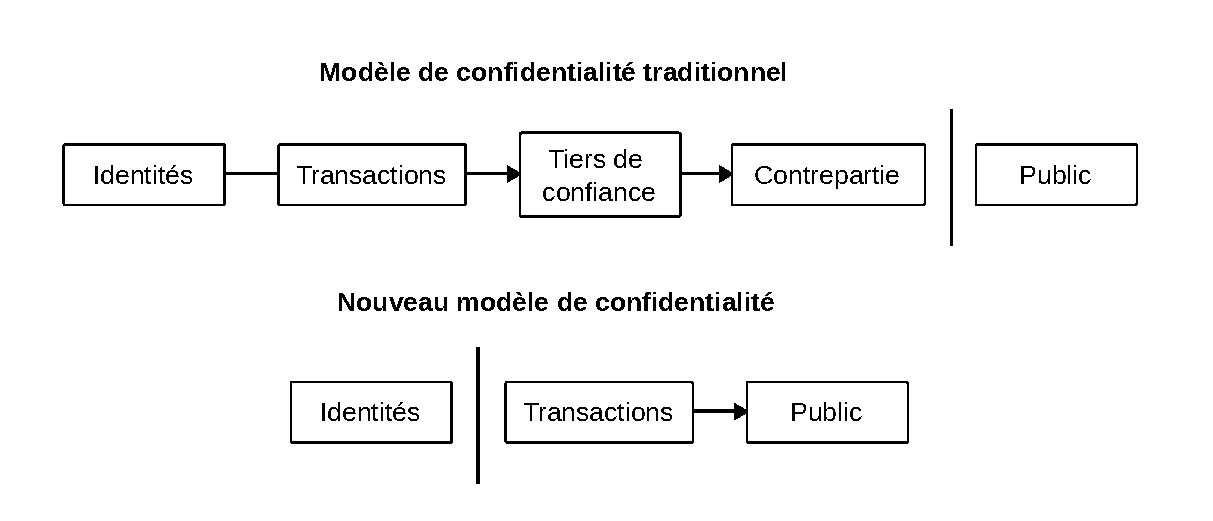
\includegraphics[scale=0.55]{img/white-paper-privacy-model-fr.eps}
  \caption{Modèle de confidentialité présenté dans le livre blanc de Bitcoin.}
\end{figure}

% Fuites d'information
Toutefois, des fuites d'information peuvent avoir lieu~: l'identité de l'utilisateur peut être dévoilée, que ce soit du fait de sa propre erreur ou de la divulgation (volontaire ou involontaire) de son interlocuteur dans l'échange. Par conséquent, nul ne peut prétendre être à l'abri de telles fuites\sendnote{Les premiers utilisateurs de Bitcoin ont ainsi été bien imprudents, à l'instar de Hal Finney qui a révélé des informations entre 2013 et 2014 permettant de déduire qu'il possédait plus de 10~000~bitcoins en 2011. -- Hal Finney, \emph{Bitcoin and me}, \wtime{19/03/2013 20:40:02 UTC}~: \url{https://bitcointalk.org/index.php?topic=155054.msg1643833\#msg1643833}~; Andy Greenberg, \eng{Nakamoto's Neighbor: My Hunt For Bitcoin's Creator Led To A Paralyzed Crypto Genius}, 25 mars 2014~: \url{https://www.forbes.com/sites/andygreenberg/2014/03/25/satoshi-nakamotos-neighbor-the-bitcoin-ghostwriter-who-wasnt/}.}. C'est pourquoi il existe des méthodes permettant de limiter leur effet et de retrouver la confidentialité en toute sérénité.

% Usage unique des adresses
La première mesure est l'usage unique des adresses. Elle consiste à générer une nouvelle clé privée et une nouvelle adresse lors de chaque paiement entrant et sortant. L'apport est de réduire l'impact de la révélation du lien avec l'identité sur la confidentialité générale~: tant que l'adresse n'est pas liée à d'autres par l'observation d'une action sur la chaîne (co-dépense par exemple), la fuite d'information se limite à cette seule adresse. Cette bonne pratique était citée dans le livre blanc\sendnote{«~Comme pare-feu supplémentaire, une nouvelle paire de clés devrait être utilisée pour chaque transaction afin de les empêcher d'être liées à un propriétaire commun. Certains liens sont toujours inévitables avec les transactions à entrées multiples, qui révèlent nécessairement que leurs entrées appartiennent au même propriétaire. Le risque est que si le propriétaire d'une clé est révélé, la liaison pourrait révéler d'autres transactions qui lui appartiennent.~» -- Satoshi Nakamoto, \eng{Bitcoin: A Peer-to-Peer Electronic Cash System}, 31 octobre 2008.} et est aujourd'hui implémentée dans tous les portefeuilles.

% Mélange de pièces
On peut également corriger les erreurs. Une des méthodes la plus connue pour procéder à ce type de correction est le mélange de pièces, qui permet de combiner ses UTXO avec d'autres utilisateurs afin de briser le lien déterministe qui existe.

% Tumblers
Le mélange de bitcoins était originellement pris en charge par des services de mixage centralisés, appelés \eng{mixers} ou \eng{tumblers}, qui recevaient les bitcoins des utilisateurs, les fusionnaient et leur renvoyaient des bitcoins communs au bout d'un certain temps, préférablement sous la forme de plusieurs transactions. Le premier mélangeur de ce type était BitLaundry, qui a été lancé en septembre 2010 par Peter Vessenes\sendnote{Peter Vessenes, \eng{Announcing: BitLaundry -- decorrelated payment service}, \wtime{01/09/2010 05:52:25 UTC}~: \url{https://bitcointalk.org/index.php?topic=963.msg11823\#msg11823}.}. Ces services permettaient d'obscurcir la provenance des bitcoins pour un observateur extérieur, mais pas pour le gérant du service, qui pouvait également voler les bitcoins au passage.  % Bitcoin Fog (2011), Silk Road

% CoinJoin
Une technique pour procéder à ce type de mélange sans devoir passer par un intermédiaire a par la suite été développée~: c'était CoinJoin, dont la description formelle a été faite en août 2013 par Gregory Maxwell\sendnote{Gregory Maxwell, \eng{CoinJoin: Bitcoin privacy for the real world}, \wtime{22/08/2013 02:32:31 UTC}~: \url{https://bitcointalk.org/index.php?topic=279249.msg2983902\#msg2983902}.}. Il s'agit d'impliquer les pièces dans une transaction jointe collaborative qui brise la correspondance entre les entrées et une partie des sorties. La transaction classique que l'on se représente est celle de plusieurs utilisateurs qui signent chacun une entrée, dont la même nombre de sorties possèdent un montant égal, et dont le reste des sorties forment les sorties complémentaires. Dans ce cas, les sorties complémentaires sont toujours liées aux entrées, contrairement aux sorties principales qui sont indiscernables les unes des autres.

\begin{figure}[ht]
  \centering
  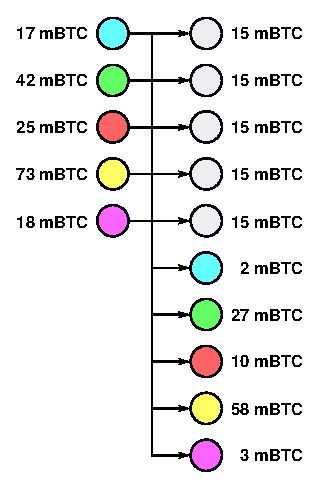
\includegraphics[scale=0.85]{img/coinjoin-transaction-5i-10o.eps}
  \caption{Exemple d'une transaction CoinJoin à 5 utilisateurs.}
  \label{fig:coinjoin-transaction}
\end{figure}

% Ensemble d'anonymat
Ces mélanges reposent sur la notion d'«~ensemble d'anonymat~» (\eng{anonymity set}) qui permet de mesurer la difficulté à faire le lien entre l'entrée et le sortie à un moment donné. On peut ainsi obtenir un score prospectif qui est le nombre de possibilités de pièces en sorties auxquelles peuvent correspondre une pièce en entrée. Dans notre exemple illustré par la figure~\ref{fig:coinjoin-transaction}, le score prospectif de la sortie au moment de la transaction est de 5. Si la pièce avait subi un nouveau mélange (comme c'est fait dans Whirlpool), alors elle aurait eu un score prospectif de 9. On peut aussi, même si c'est plus rare, calculer un score rétrospectif qui correspond au nombre de potentielles pièces en entrée auxquelles peut être liée une sortie particulière, qui est également de 5 dans le cas de notre transaction simple, mais qui peut être largement supérieur en cas de remélanges fréquents. \sendnote{Loïc Morel, \emph{Comprendre et utiliser le CoinJoin sur Bitcoin}, 19 juillet 2022~: \url{https://www.pandul.fr/post/comprendre-et-utiliser-le-coinjoin-sur-bitcoin}.}

% Coordinateur
Pour gérer le tout, le système fait utilise généralement un protocole qui permet aux participants d'être mis en relation anonymement par le biais d'un coordinateur sans risque de fuite d'information ou de vol des fonds. Le plus connu est ZeroLink, développé par Adam Ficsor (\texttt{nopara73}) et \texttt{TDevD} en août 2017, qui est un protocole qui utilise le procédé de signature aveugle de David Chaum\sendnote{nopara73, TDevD, \eng{ZeroLink: The Bitcoin Fungibility Framework}, 14 août 2017~: \url{https://github.com/nopara73/ZeroLink/tree/32ad53927a343383534bea28fffb098af65fe62a}.}. C'est dans ce sens qu'on parle parfois de CoinJoin chaumien (\eng{Chaumian CoinJoin}). Une implémentation classique de cette idée a été réalisée par Whirlpool et par Wasabi 1.0. Des variantes (CoinShuffle, CoinShuffle++, CashShuffle, CashFusion) ont été implémentées sur des variantes de Bitcoin comme Decred ou Bitcoin Cash. Plus récemment le portefeuille Wasabi a intégré Wabisabi qui permet de réaliser des mélanges avec des valeurs arbitraires en sortie, ce qui complique l'estimation de la confidentialité apportée mais mais évite d'avoir à gérer les sorties complémentaires d'une manière séparée.

% PayJoin
Pour autant, les transactions collaboratives ne se limitent pas au CoinJoin. Il existe par exemple une autre méthode, appelée PayJoin, qui permet au commerçant de réaliser un mélange avec le client au moment du paiement, en impliquant une pièce en entrée. Cela a pour effet de fausser l'analyse de chaîne en faisant croire à l'observateur extérieur qu'un seul utilisateur a réuni ses pièces en entrée.

Reprenons notre exemple d'Alice qui paie 7~mBTC à Bob en réunissant deux pièces de 6 et 2~mBTC afin d'atteindre un montant suffisant en entrée. Dans ce cas, les deux entrées sont supposément liées entre elles (heuristique de co-dépense) et liées à la sortie de 1~mBTC (heuristique de la sortie complémentaire). Dans ce cas, PayJoin consiste à faire en sorte que le commerçant inclue une ou plusieurs pièces en entrée et augmente d'autant le montant de la sortie qui lui est destinée, 7~mBTC par exemple. La transaction est représentée sur la figure~\ref{fig:payjoin-transaction}.

\begin{figure}[ht]
  \centering
  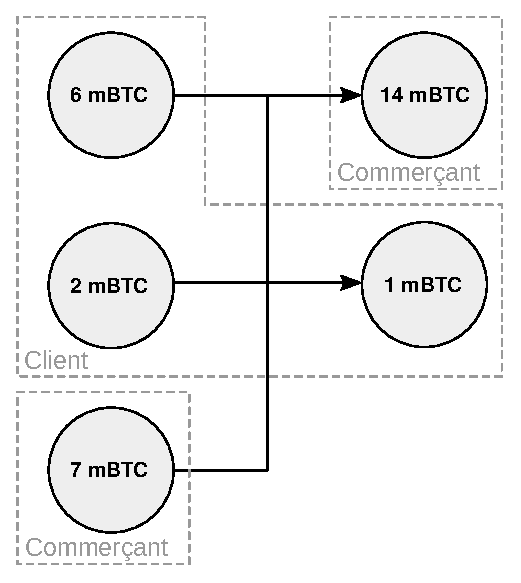
\includegraphics[scale=0.75]{img/payjoin-transaction-3i-2o.eps}
  \caption{Exemple d'une transaction PayJoin.}
  \label{fig:payjoin-transaction}
\end{figure}

Cette technique a été conceptualisée en 2018 sous la forme du protocole Bustapay proposé dans le BIP-79, qui n'a jamais été mis en application. Elle a est néanmoins implémentée aujourd'hui par l'intermédiaire du protocole de paiement Pay-to-EndPoint (P2EP) implémenté dans plusieurs portefeuilles\sendnote{Adam Ficsor, \eng{Pay To EndPoint}, 31 juillet 2018~: \url{https://nopara73.medium.com/pay-to-endpoint-56eb05d3cac6}.} et des transactions Stowaway du Samourai Wallet\sendnote{Samourai Wallet, \eng{Stowaway}~: https://samouraiwallet.com/stowaway}.

% CoinSwap
Enfin une dernière méthode est Coinswap, qui est un procédé développé par Chris Belcher, permettant à deux utilisateurs ou plus d'échanger leurs pièces sans qu'ils aient besoin de se faire confiance et sans que cette opération laisse une trace particulière sur la chaîne\sendnote{Chris Belcher, \eng{Design for a CoinSwap Implementation for Massively Improving Bitcoin Privacy and Fungibility}, 25 mai 2020~: \url{https://gist.github.com/chris-belcher/9144bd57a91c194e332fb5ca371d0964}.}.

\section*{D'autres techniques de confidentialité}
\addcontentsline{toc}{section}{D'autres techniques de confidentialité}

% Dandelion. Dandelion++.

% Autres techniques
Outre le mélange de pièces simple consistant à brouiller les pistes qu'un observateur externe pourrait suivre, il existe un certain nombre de techniques qui permettent d'améliorer la confidentialité de Bitcoin. Celles-ci requièrent souvent la modification du protocole de base et font des compromis, raison pour laquelle elles ne sont pas forcément mises en œuvre.

% Satoshi et l'innovation
Ces techniques ont été développées dans les années qui ont suivi l'apparition de Bitcoin, notamment sur le forum Bitcointalk. N'étant pas un cryptographe universitaire, Satoshi Nakamoto s'est surtout focalisé sur la robustesse du système lorsqu'il l'a conçu et n'a pas cherché à y inclure des techniques avancées. Cependant, il était preneur de tout ce qui pourrait permettre de lancer une «~mise en œuvre de Bitcoin bien meilleure, plus facile et plus pratique\sendnote{Satoshi Nakamoto, \eng{Re: Not a suggestion}, \wtime{11/08/2010 00:14:22 UTC}~: \url{https://bitcointalk.org/index.php?topic=770.msg8637\#msg8637}.}~».

% Discussion entre Red et Satoshi sur des façons d'améliorer le protocole : https://bitcointalk.org/index.php?topic=770.0

% --- Signatures de cercle ---

La première technique de cet ordre est le procédé de signature de cercle (\eng{ring signature}) a été formalisé en 2001 par Ronald Rivest, Adi Shamir et Yael Tauman\sendnote{Ronald L. Rivest, Adi Shamir, Yael Tauman, \eng{How to Leak a Secret}, 2001~: \url{https://people.csail.mit.edu/rivest/pubs/RST01.pdf}.}. Celui-ci se base sur le procédé de signature de groupe, introduite par David Chaum et Eugène van Heyst en 1991, qui permettait à chaque membre d'un groupe de signer un message au nom du groupe sans que ce membre puisse être identifié par un vérificateur externe, mais qui reposait sur un gestionnaire central. La signature de cercle innovait par le fait qu'elle ne requérait pas de gestionnaire central, pas de procédure d'installation et pas de coordination, et qu'elle ne permettait pas à un membre de révoquer son anonymat.

% Application
Au sein de la cryptomonnaie, le principe est le suivant~: pour chaque pièce en entrée de la transaction, le signataire rassemble plusieurs autres pièces disponibles sur la chaîne (appelées sorties leurres ou \eng{decoy outputs}), utilise leurs clés publiques et signe avec sa clé privée. Il fournit également une image de clé (correspondant à la pièce) qui est écrite sur la chaîne et qui permet de garantir que la même pièce n'est pas dépensée deux fois. Plus le cercle implique de sorties, plus l'ensemble d'anonymat est grand. L'utilisation des sorties transactionnelles en tant que leurres oblige les nœuds à conserver l'ensemble de ces sorties, puisqu'on ne peut pas savoir laquelle a été réellement dépensée.

% Satoshi "group signature": https://bitcointalk.org/index.php?topic=770.msg9074#msg9074

% --- Adresses furtives ---

% Stealth Addresses, 2011-2014
La deuxième technique est le procédé des adresses furtives, qui a été décrit en 2011 par Nicolas van Saberhagen et qui a été formalisé en 2014 par Peter Todd dans le cadre de Bitcoin\sendnote{Nicolas van Saberhagen (ByteCoin), \eng{Untraceable transactions which can contain a secure message are inevitable}, \wtime{17/04/2011, 02:34:24 UTC}~: \url{https://bitcointalk.org/index.php?topic=5965.msg87757\#msg87757}~; Peter Todd, \eng{[Bitcoin-development] Stealth Addresses}, \wtime{06/01/2014 12:03:38 UTC}~: \url{https://lists.linuxfoundation.org/pipermail/bitcoin-dev/2014-January/004020.html}.}. Il utilise essentiellement le schéma d’échange de clés Diffie-Hellman basé sur les courbes elliptiques, abrégé en ECDH, afin de permettre de générer des adresses à usage unique.

% Fonctionnement
Le fonctionnement de base est le suivant. Le destinataire génère une clé privée et en déduit une clé publique qu'il transmet sous la forme d'une méta-adresse. L'expéditeur génère une clé privée éphémère, appelée clé privée de la transaction, et calcule la clé publique correspondante. Ils peuvent calculer un secret partagé à partir de leur clé privée et de la clé publique de l'autre (ECDH). L'expéditeur utilise ce secret et la clé publique du destinataire pour construire une adresse à usage unique et y envoie les fonds, que seul le destinataire peut dépenser sous condition de connaître la clé publique de transaction (qui peut être stockée dans une sortie NULLDATA). Au lieu d'utiliser une seule paire de clés, le destinataire peut également en utiliser deux pour qu'elles aient des rôles séparés~: les clés d'inspection (\eng{view keys}) et les clés de dépense (\eng{spend key}). La clé privée d'inspection est le seul élément non public qui intervient dans la construction de l'adresse côté destinataire et sert donc à identifier les sorties correspondant à l'adresse en question. La clé privée de dépense est celle qui sert, comme son nom l'indique clairement, à dépenser les fonds.\sendnote{En termes mathématiques, si on note $r$ et $R$ les clés éphémères de transaction, $v$ et $V$ les clés d'inspection et $k$ et $K$ les clés de dépense, alors la méta-adresse est $M = (K, V)$, le secret partagé est~:

\[
S = r~V = r~v~G = v~r~G = v~R
\]

et la clé publique de réception est~:

\[
P = K + H(S)~G~.
\]

Le destinataire peut aussi n'utiliser qu'une seule paire de clés $(k, K)$. Dans ce cas, $M = K$.}

Si elle est implémentée de manière externe au protocole, cette méthode a le désavantage d'exiger de balayer l'entièreté de la chaîne de blocs pour savoir si on a reçu un paiement. C'est dans l'idée d'éviter cette charge que le BIP-47 a été proposé.

% Alice : clés de transaction, Bob : clés de dépense et d'inspection

% BIP-47, 2015
Une autre méthode apparentée et plus évoluée est celle des codes de paiement réutilisables (\eng{reusable payment codes}) formalisés dans le BIP-47\sendnote{Justus Ranvier, \eng{Reusable Payment Codes for Hierarchical Deterministic Wallets}, 24 avril 2015~: \url{https://github.com/bitcoin/bips/blob/master/bip-0047.mediawiki}.}, qui a été implémentée sous la forme des PayNyms dans les portefeuilles Samourai et Sparrow. Les codes de paiement de deux participants permettent de dériver les adresses de réception, grâce à la dérivation de clés. Il faut qu'ils connaissent leurs codes de paiement respectifs. La transmission du code de paiement de l'expéditeur se fait de manière chiffrée au travers d'une transaction de notification envoyée à l'adresse du destinataire. Ce schéma a pour gros défaut d'exiger la réalisation d'une transaction (et donc de payer des frais) pour ajouter un destinataire possible.

% Silent Payments, 2022
Une autre variante est le procédé des paiements silencieux (\eng{silent payments}), proposé en 2022 par Ruben Somsen\sendnote{Ruben Somsen, \eng{Silent Payments}, 13 mars 2022~: \url{https://gist.github.com/RubenSomsen/c43b79517e7cb701ebf77eec6dbb46b8}.}, qui évite la charge de la notification en utilisant la clé publique de l'une des entrées de la transaction, et réduit la charge du balayage de la chaîne, en se limitant à l'ensemble des UTXO ou un sous-ensemble comme les sorties P2TR par exemple.

% CryptoNote, 2013
La technique des signatures de cercle et le procédé des adresses furtives ont été combinés en 2013 dans le concept de cryptomonnaie CryptoNote par un individu se faisant appeler Nicolas van Saberhagen\sendnote{Nicolas van Saberhagen, \eng{CryptoNote v2.0}, 17 octobre 2013~: \url{http://cryptonote.org/whitepaper.pdf}~; archive~: \url{https://web.archive.org/web/20140529235502/http://cryptonote.org/whitepaper.pdf}.}. Dans celui-ci, les nœuds ont besoin de conserver l'ensemble des sorties transactionnelles (car, comme on l'a dit, on ne peut pas savoir quelle sortie a été dépensée) et chaque portefeuille a besoin de balayer l'ensemble de ces sorties pour voir s'il a reçu un paiement. Le fait que les \eng{stealth addresses} soient intégrées au protocole permet de publier la clé publique éphémère directement dans la transaction (ce qui en fait une clé de transaction) et d'éviter la nécessité de notification. Le concept a été implémenté initialement dans le très douteux Bytecoin en mars 2014, avant de se retrouver dans Monero en avril, qui en est aujourd'hui le représentant principal, mettant notamment en place des signatures de cercle à \textcolor{darkgray}{16 membres}.

% Le système imposait de séparer les fonds en différentes valeurs~: pièces de 10 unités, de 2 unités, etc.

% --- Montants confidentiels ---

% Confidential Transactions, 2013-2015
La troisième technique est le procédé des \eng{Confidential Transactions} («~transactions confidentielles~» en français, abrégés en CT), qui permet de dissimuler les montants impliqués dans les échanges des utilisateurs, et qui devrait par conséquent être plutôt appelé \eng{Confidential Amounts}. Le procédé a été décrit par Adam Back en 2013 et formalisé par Gregory Maxwell en 2015\sendnote{Adam Back, \eng{bitcoins with homomorphic value (validatable but encrypted)}, \wtime{October 01, 2013, 02:19:53 PM}~: \url{https://bitcointalk.org/index.php?topic=305791.msg3277431\#msg3277431}~; Gregory Maxwell, \eng{Confidential Transactions}, 2015~: \url{https://web.archive.org/web/20150628230410/https://people.xiph.org/~greg/confidential_values.txt}.}. Il impose à chaque sortie transactionnelle de contenir un engagement de Perdersen ou \eng{Pedersen commitment}, qui lie la pièce à la clé publique du destinataire sans la dévoiler, et une preuve de portée ou \eng{range proof}, qui est une preuve à divulgation nulle de connaissance démontrant la validité du montant sans le révéler.

% Implémentation dans Monero
Les Confidential Transactions ont été ajoutée à Monero grâce au travail de Shen Noether\sendnote{Shen Noether, \eng{Ring Confidential Transactions}, 2015~: \url{https://eprint.iacr.org/2015/1098.pdf}.}.  RingCT, qui permet de cacher les montants échangés, a ainsi été ajouté au protocole en janvier 2017 et a été rendu obligatoire en septembre de la même année. Il alourdissait les transactions par rapport à des transactions classiques. Néanmoins, depuis octobre 2018, ce compromis a été mitigé grâce à l'implémentation des bulletproofs\sendnote{\eng{Bulletproofs: Short Proofs for Confidential Transactions and More}, \url{https://eprint.iacr.org/2017/1066.pdf}.}, qui allège le fardeau des preuves de portée, ce qui a permis de réduire de 80~\% la taille des transactions.

% Dans Monero, les signatures de cercle protègent l'anonymat de l'expéditeur, les adresses furtives améliorent la confidentialité du destinataire et RingCT dissimule les montants publics des transactions.

% Mimblewimble
Un autre concept faisant usage des Confidential Transactions est Mimblewimble. Celui-ci a été proposé le 1\ier{} août 2016 par un inconnu se faisant appeler Tom Elvis Jedusor au sein du canal IRC \texttt{\#bitcoin-wizards}\sendnote{Bitcoin-wizards logs, 1\ier{} août 2016~: \url{https://gnusha.org/bitcoin-wizards/2016-08-01.log}} où il partageait un lien vers un texte descriptif hébergé sur Tor\sendnote{Tom Elvis Jedusor, \eng{Mimblewimble}, 19 juillet 2016~: \url{http://5pdcbgndmprm4wud.onion/mimblewimble.txt}~; archive~: \url{https://download.wpsoftware.net/bitcoin/wizardry/mimblewimble.txt}. -- Le nom du concept et le pseudonyme du créateur sont issus de l'univers d'Harry Potter~: Mimblewimble est la formule du sortilège à la langue de Plomb qui interdit à l'adversaire de parler en faisant des nœuds avec sa langue (Mimblewimble est censé «~empêcher la chaîne de blocs de parler des informations personnelles de ses utilisateurs~») et Tom Elvis Jedusor est le vrai nom de Voldemort dans la traduction française.}. Mimblewimble a attiré l'attention de certains développeurs de Bitcoin, dont le mathématicien Andrew Poelstra qui a en fait une description plus avancée dans un papier daté du 6 octobre 2016\sendnote{Andrew Poelstra, \eng{Mimblewimble}, 6 octobre 2016~: \url{https://download.wpsoftware.net/bitcoin/wizardry/mimblewimble.pdf}.}.

% Description technique
L'apport de Mimblewimble est de condenser l'historique des transactions en chamboulant la structure des transactions. Il repose sur trois primitives cryptographiques~: les Confidential Transactions, qui cachent les montants, les signatures agrégées à sens unique (OWAS), qui permettent de combiner les transactions au sein d'un bloc\sendnote{Horas Yuan Mouton, \eng{Increasing Anonymity in Bitcoin}, 9 septembre 2013~: \url{https://www.dropbox.com/s/nkh22cibel8stb4/horasyuanmouton.pdf}~; archive~: \url{https://download.wpsoftware.net/bitcoin/wizardry/horasyuanmouton-owas.pdf}.}, et le sectionnage des transactions (\eng{transaction cut-through}), qui permet de supprimer les sorties transactionnelles intermédiaires\sendnote{Gregory Maxwell, \eng{Transaction cut-through}, \wtime{26/08/2013 22:17:19 UTC}~: \url{https://bitcointalk.org/index.php?topic=281848.msg3014613\#msg3014613}.}. Cette réduction, qui améliore la confidentialité du système de manière relativement légère, se fait au prix de la programmabilité, rendue impossible directement.

% Mises en œuvre de Mimblewimble : Grin, Beam et Litecoin
Mimblewimble a été mis en œuvre de manière native au sein du système Grin développé par Ignotus Peverell à partir d'octobre 2016 et lancé le 15 janvier 2019. Une autre implémentation, également lancée en janvier 2019, était le réseau Beam. Mimblewimble a également été intégré à Litecoin le 20 mai 2022 sous la forme d'un soft fork de bloc auxiliaire, appelé MWEB pour \eng{MimbleWimble via Extension Blocks}. % bloc 2~265~984

% --- Méthodes basées sur des zero-knowledge proofs ---

% Zerocoin, Zerocash
Enfin, d'autres techniques basées sur des preuves à divulgation nulle de connaissance existent. Les plus connues ont été popularisées au travers de deux protocoles rendus publics en 2013 et en 2014 par Matthew Green et ses étudiants~: Zerocoin et Zerocash\sendnote{Ian Miers, Christina Garman, Matthew Green, Aviel D. Rubin, \eng{Zerocoin: Anonymous Distributed E-Cash from Bitcoin}, 2013~: \url{https://ieeexplore.ieee.org/document/6547123}~; Eli Ben Sasson, Alessandro Chiesa, Christina Garman, Matthew Green, Ian Miers, Eran Tromer, Madars Virza, \eng{Zerocash: Decentralized Anonymous Payments from Bitcoin}, 2014~: \url{https://ieeexplore.ieee.org/document/6956581}.}. Le premier protocole, Zerocoin, permet de cacher la provenance des fonds. Le second protocole permet de cacher la provenance, la destination et les montants, au moyen de zk-SNARK (\eng{Zero-Knowledge Succinct Non-Interactive Arguments of Knowledge} ou «~argument de connaissance succinct et non interactif à divulgation nulle de connaissance~» en français).

% Mise en œuvre : Zcoin, Zcash
Zerocoin a été implémenté dans Zcoin en septembre 2016. À partir de 2019, Zcoin s'est progressivement éloigné du Zerocoin en adoptant les protocole Sigma et Lelantus. Il est devenu Firo en 2020. Zerocash a lui été implémenté au sein du système Zcash en octobre 2016. L'utilisation de preuves à divulgation nulle de connaissance demande une configuration de confiance des paramètres publics. Au contraire des développeurs de Zcoin qui ont fait le choix d'utiliser des paramètres connus, ceux de Zcash ont choisi d'organiser un évènement, appelée «~\eng{The Ceremony}~», dans le but de générer ces paramètres. Cette cérémonie a eu lieu du 21 au 23 octobre 2016 et a réuni six participants~: Andrew Miller, Peter Van Valkenburgh, Zooko Wilcox-O'Hearn, Derek Hinch, Peter Todd et surtout Edward Snowden sous le pseudonyme de John Dobbertin\sendnote{Zooko Wilcox-O'Hearn, \eng{The Design of the Ceremony}, 26 octobre 2016~: \url{https://electriccoin.co/blog/the-design-of-the-ceremony/}.}. Cette configuration de confiance a été rendu inutile en 2022 avec l'adoption du protocole Halo.

% Compromis
De manière générale, tous ces procédés supposent des compromis au niveau de la scalabilité (les preuves sont plus lourdes qu'une simple signature), au niveau de l'auditabilité (ne pas voir les montants implique de devoir faire entièrement confiance aux procédés et à leur implémentation) et au niveau de la programmabilité (programmer des pièces s'oppose au fait de les rendre indistinctes). C'est pourquoi ils ont tous été mis en œuvre dans des versions alternatives de Bitcoin et pas dans sa version principale (BTC), sa communauté étant plus conservatrice par nature.

\section*{Une machine complexe}
\addcontentsline{toc}{section}{Une machine complexe}

Bitcoin forme ainsi une machine qui peut sembler, à première vue, complexe. Cette complexité relative s'explique par ses objectifs et par les évènements qui ont jalonné son histoire technique. Son but premier -- être une monnaie -- est à l'origine de la représentation des bitcoins en circulation par des sorties transactionnelles non dépensées, qui est à la fois plus facile à paralléliser et plus confidentielle. Il est aussi possible de mettre en œuvre le mélange de pièces et des techniques cryptographiques pour améliorer cette confidentialité.

De plus, la volonté de Satoshi d'automatiser divers mécanismes lui a fait intégrer un véritable système de programmation au sein du prototype. Celui-ci permet de mettre en place des contrats autonomes, ou \eng{smart contracts}, qui exécutent des interactions financières complexes entre plusieurs participants. Il facilite aussi, indirectement, l'inscription de données arbitraires sur la chaîne. Ces deux utilisations -- contractuelle et notariale -- forment les deux cas d'usage secondaires de Bitcoin, dont nous parlerons dans le prochain chapitre.
% Copyright (c) 2023 Ludovic Lars
% This work is licensed under the CC BY-NC-SA 4.0 International License

\chapter{Les contrats autonomes}
\label{ch:contrats}
\label{enotezch:13}

\lettrine[]{U}n contrat autonome, de l'anglais \eng{smart contract}, est un programme informatique dont l'exécution ne nécessite pas l'intervention d'un tiers de confiance. On parle aussi de contrat auto-exécutable ou de contrat intelligent (traduction littérale). Chaque contrat est constitué de clauses qui sont des conditions de dépense spécifiques.

Bitcoin constitue la première implémentation concrète d'un système hébergeant des contrats autonomes, par le biais de son système de programmation interne qui met en œuvre des scripts au sein des transactions. Il permet d'exécuter une variété de contrats allant du compte multisignatures au canal de paiement, en passant par le dépôt fiduciaire. L'ouverture apportée par cette possibilité facilite l'inscription de données arbitraires sur la chaîne, un cas d'utilisation strictement non monétaire du protocole.

\section*{Les contrats simples}
\addcontentsline{toc}{section}{Les contrats simples}

% Origine du concept
La notion de contrat autonome\sendnote{L'appellation «~contrat autonome~» visant à traduire \eng{smart contract} a été proposée par Jacques Favier, Adli Takkal-Bataille et Benoît Huguet dans \emph{Bitcoin~: Métamorphoses} (pp. 105--107) en 2018.} a germé au sein du mouvement cypherpunk dans les années 1990. Elle a été exposée par Nick Szabo en 1994, qui la définissait comme suit~:

\begin{quote}
«~Un contrat autonome est un protocole de transaction informatisé qui exécute les termes d'un contrat. Les objectifs généraux de la conception de contrats autonomes sont de satisfaire les conditions contractuelles courantes (telles que les conditions de paiement, les privilèges, la confidentialité et même l'exécution), de minimiser les exceptions, tant malveillantes qu'accidentelles, et de minimiser le besoin d'intermédiaires de confiance\sendnote{Nick Szabo, \eng{Smart Contracts}, 1994, archive~: \url{https://web.archive.org/web/20011102030833/http://szabo.best.vwh.net:80/smart.contracts.html}.}.~»
\end{quote} % "A smart contract is a computerized transaction protocol that executes the terms of a contract. The general objectives of smart contract design are to satisfy common contractual conditions (such as payment terms, liens, confidentiality, and even enforcement), minimize exceptions both malicious and accidental, and minimize the need for trusted intermediaries."

% Transfert de valeur et contrats plus complexes
Le transfert de valeur constitue le cas le plus simple de contrat autonome, ne contenant qu'une seule clause~: la fourniture d'une signature numérique correspondant à une clé publique donnée. Mais une multitude d'autres contrats peuvent être implémentés sur Bitcoin, à tel point qu'il est impossible d'en dresser une liste exhaustive. Nous nous contenterons ici d'en décrire quelques exemples pour expliquer comment ils peuvent être mis en place. Voyons d'abord les cas spécifiques du compte multisignatures, du dépôt fiduciaire, du financement participatif et de l'échange atomique.

% --- Compte multisignatures ---

\subsection{Le compte multisignatures} Le compte multisignatures est un compte partagé entre plusieurs entités. Il se base sur le schéma de signature multipartite décrit dans le chapitre~\ref{ch:rouages}, dans lequel la dépense des fonds demande M signatures parmi N participants (ce qu'on appelle «~M-parmi-N~» ou «~M-of-N~» en anglais). Par exemple, la dépense depuis un compte 2-parmi-3 exige que 2 personnes parmi 3 participants prédéterminés produisent une signature valide, peu importe l'identité précise de ces personnes.

%  Apport
Ce type de contrat est utile pour avoir un compte joint entre époux (2 parmi 2), pour faciliter la détention par une entreprise (3 associés parmi 7 par exemple) ou pour améliorer la conservation de bitcoins en général. Les plateformes d'échange utilisent notamment ce type de contrat pour conserver leurs avoirs. En novembre 2023, la deuxième adresse la plus riche du monde en 2023 était ainsi l'adresse multisignatures 3-parmi-5 de Bitfinex contenant plus de 178~000~BTC\sendnote{L'adresse multisignatures 3-parmi-5 de Bitfinex est \longstring{bc1qgdjqv0av3q56jvd82tkdjpy7gdp9ut8tlqmgrpmv24sq90ecnvqqjwvw97}.}.

% --- Dépôts fiduciaires ---

\subsection{Le dépôt fiduciaire} Le dépôt fiduciaire, appelé \eng{escrow} en anglais, est une méthode basée sur le recours à un tiers de confiance, comme un notaire, pour sécuriser une transaction entre deux parties qui se méfient l'une de l'autre. L'utilisation de la programmabilité de Bitcoin permet de diminuer le pouvoir du tiers en incluant une limite dans la clause qui le concerne. Ce type de contrat repose sur deux briques techniques de base~: la signature multipartite et les verrous temporels.

% Fonctionnement
Prenons l'exemple de deux personnes qui ne se connaissent pas, Alice et Bob, et qui veulent réaliser une transaction en ligne\pagenote{«~l'exemple de deux personnes qui ne se connaissent pas, Alice et Bob, et qui veulent réaliser une transaction en ligne~»~: Une description de ce contrat est faite dans le BIP-65~: \url{https://github.com/bitcoin/bips/blob/master/bip-0065.mediawiki}.}~: Alice est l'acheteuse, Bob le vendeur. Les deux parties font appel à un intermédiaire de confiance, Lenny, avec qui elles créent le contrat de dépôt fiduciaire. Alice y envoie les fonds et attend de recevoir le bien. Deux clauses peuvent alors être activées~:

\begin{itemize}
\item Le règlement à l'amiable~: le contrat est déverrouillé par les signatures des deux parties, qui peuvent choisir d'envoyer les fonds vers Bob (réussite de l'échange) ou bien de rembourser Alice (échec de l'échange)~;
\item Le litige~: après une période prédéterminée (par exemple 30 jours), le contrat est déverrouillé par la signature de Lenny et celle de l'une des deux parties~; dans ce cas, Lenny se charge de déterminer qui est la partie honnête et de lui envoyer les fonds.
\end{itemize}

\begin{figure}[ht]
  \centering
  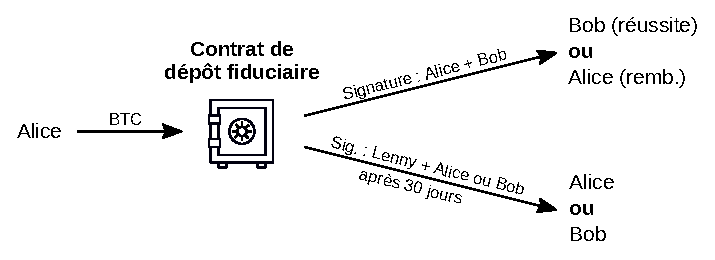
\includegraphics[scale=0.9]{img/escrow-contract.eps}
  \caption{Contrat de dépôt fiduciaire.}
  \label{fig:escrow-contract}
\end{figure}

% Apports
Ce fonctionnement, décrit sur la figure~\ref{fig:escrow-contract}, incite d'une part les deux parties à coopérer pour ne pas perdre de temps, et empêche d'autre part la collusion de la tierce partie (Lenny) avec l'une des deux autres avant le délai prévu (30 jours ici). Le recours à la confiance est ainsi minimisé autant que possible.

% Historique et mise en œuvre
Ce type de contrat était soutenu par Satoshi Nakamoto dans le livre blanc\sendnote{«~Les acheteurs pourraient être facilement protégés par la mise en œuvre de mécanismes de dépôt fiduciaire routiniers.~» -- Satoshi Nakamoto, \eng{Bitcoin: A Peer-to-Peer Electronic Cash System}, 31 octobre 2008.}. En effet, l'irréversibilité des transferts dans Bitcoin offrait peu de garantie pour les commerçants, et le dépôt fiduciaire permettait d'atténuer le problème. C'est typiquement ce genre de mécanisme qui intervient aujourd'hui dans les plateformes de change de pair à pair comme Bisq ou Hodl Hodl, même si l'implémentation diffère de ce qui est présenté ici.

% --- Financement participatif ---

\subsection{Le financement participatif} Le financement participatif consiste à faire appel au grand public pour contribuer au soutien d'un projet, par opposition au financement par prêt bancaire ou par levée de fonds auprès des professionnels du capital-risque. Il s'agit le plus souvent d'un accord informel entre le promoteur du projet et le public ayant pour but de soutenir la création d'un bien commun, qui profite à tous. Dans Bitcoin, il est possible d'exécuter cet accord par le biais de promesses de paiement résiliables qui ne sont pas soumises à l'arbitraire d'un tiers de confiance.

% Fonctionnement
D'un point de vue technique, il s'agit de créer une transaction dite \eng{anyone-can-pay} («~tout le monde peut payer~») où la signature de chaque contributeur ne prend en compte que la sortie transactionnelle de la levée de fonds et l'entrée du contributeur en question, donnant la possibilité d'ajouter des entrées (voir figure~\ref{fig:sighash-anyonecanpay}). La transaction résultante n'est valide que si le montant en entrée atteint le montant indiqué en sortie, de sorte que les contributeurs conservent le contrôle de leurs fonds jusqu'à la réalisation du paiement total et peuvent se retirer à tout moment.

\begin{figure}[ht]
  \centering
  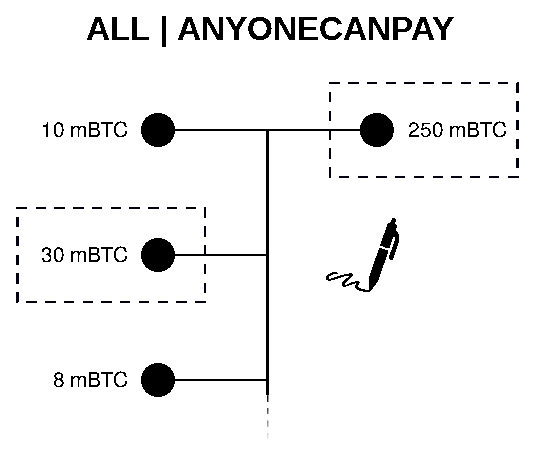
\includegraphics[scale=0.65]{img/sighash-anyonecanpay.eps}
  \caption{Transaction de financement participatif.}
  \label{fig:sighash-anyonecanpay}
\end{figure}

% Apport, historique et mise en œuvre
Dans le monde du logiciel libre, ce type de financement participatif est particulièrement important, car il n'y a pas de privilège lié à l'écriture du code qui permette de gagner sa vie par la vente de licences. C'est encore plus vrai dans le monde de la cryptomonnaie qui dépend fortement du bon maintien des implémentations logicielles. C'est pourquoi Mike Hearn, qui s'intéressait de près aux capacités de programmation de Bitcoin, s'est vite approprié cette possibilité pour déployer de tels «~contrats de garantie\pagenote{«~contrats de garantie~»~: Mike Hearn, \eng{Bitcoin Wiki: Contracts}, 23 juin 2011~: \url{https://en.bitcoin.it/wiki/Contract\#Example_3:_Assurance_contracts}~: «~Un contrat de garantie est une manière de financer la création d'un bien public, c'est-à-dire d'un bien qui, une fois créé, bénéficie à tous gratuitement. L'exemple typique est celui d'un phare~: bien que tout le monde puisse être d'accord sur le fait qu'il doit être construit, c'est bien trop cher pour justifier qu'un marin individuel en construise un, étant donné qu'il bénéficiera à tous ses concurrents. Une solution est que tout le monde promette de payer pour la création du bien public, de sorte à ce que les promesses soient appliquées seulement si la valeur totale des promesses dépasse le coût de création. Si le nombre de personnes qui contribuent n'est pas assez élevé, personne ne doit payer quoi que ce soit.~»}~» (\eng{assurance contracts}) permettant de financer les biens publics. Il a mis le concept en œuvre au sein de son application Lighthouse, dont une version fonctionnelle est sortie en 2015, qui avait pour but de faciliter le soutien communautaire des projets de l'écosystème. Avec le déclenchement de la guerre des blocs, ce projet a été mis de côté par Hearn et a fini par être abandonné. Le procédé a été néanmoins repris sur Bitcoin Cash en 2020 par l'intermédiaire de Flipstarter, qui a permis de lever d'importantes sommes pour le financement de l'infrastructure logicielle du protocole\pagenote{«~Flipstarter~»~: Ludovic Lars, \emph{Flipstarter, le financement participatif pour Bitcoin Cash}, 24 avril 2020~: \url{https://viresinnumeris.fr/flipstarter-financement-participatif-bitcoin-cash/}.}. % June 2011: "An assurance contract is a way of funding the creation of a public good, that is, a good which once created anyone can benefit from for free. The standard example is a lighthouse: whilst everyone may agree that one should be built, it's too expensive for an individual sailor to justify building one given that it will also benefit all his competitors. One solution is for everyone to pledge money towards the creation of the public good, such that the pledges are only committed if the total value of all pledges is above the cost of creation. If not enough people contribute, nobody has to pay anything."

% --- Échange atomique ---

\subsection{L'échange atomique} L'échange atomique (\eng{atomic swap}) est une manière sûre d'échanger deux cryptomonnaies fonctionnant sur des chaînes de blocs différentes, sans passer par un intermédiaire de confiance. L'adjectif «~atomique~» se rapporte à la nature insécable (en grec ancien \foreignlanguage{greek}{ἄtomos}, átomos) de l'échange~: soit les deux parties transfèrent leur dû, soit il ne se passe rien. Le concept a été décrit par Sergio Lerner et Gregory Maxwell en juillet 2012 sur le forum Bitcointalk\sendnote{Sergio Demian Lerner, \eng{P2PTradeX: P2P Trading between cryptocurrencies}, \wtime{05/07/2012 23:49:48 UTC}~: \url{https://bitcointalk.org/index.php?topic=91843.msg1011737\#msg1011737}~; Gregory Maxwell, \eng{Re: P2PTradeX: P2P Trading between cryptocurrencies}, \wtime{06/07/2012 02:17:02 UTC}~: \url{https://bitcointalk.org/index.php?topic=91843.msg1011956\#msg1011956}.}.

% Fonctionnement
L'échange atomique repose sur le concept de contrat verrouillé par une empreinte et par un temps, appelé HTLC par abréviation du terme anglais \eng{Hash Time Locked Contract}. Celui-ci est un contrat à deux clauses, c'est-à-dire que les fonds peuvent être déverrouillés à deux conditions\sendnote{Pour assurer la bonne exécution du contrat (éviter le remplacement de la transaction durant l'attente de confirmation), des clés publiques sont assignées à chacune de ces conditions de sorte qu'une signature est systématiquement demandée au destinataire des fonds.}~:

\begin{itemize}
\item L'accord mutuel~: la révélation d'un secret qui est haché par une fonction de hachage et comparé à l'empreinte (\eng{hash}) inscrite dans le contrat~;
\item Le litige~: l'attente d'un certain temps (\eng{time}) de verrouillage déterminé dans le contrat.
\end{itemize}

% Atomic Swap HTLC (AtomicDEX, 2019, BCH side)
% txid: 30eac387087d795a5c38097383e203a4c27374c07161d6720f0708910283b830
%
% IF
%   <expiry_date> CHECKLOCKTIMEVERIFY DROP
%   <bob_pubkey> CHECKSIG
% ELSE
%   SIZE <20> EQUALVERIFY
%   HASH160 <H(s)> EQUALVERIFY
%   <alice_pubkey> CHECKSIG
% ENDIF

% Préliminaires
Considérons l'exemple d'un échange atomique entre Alice, qui possède du BTC, et Bob, qui possède du LTC. Alice (\eng{maker}) propose d'échanger 0,03 BTC pour 10~LTC, à un taux de change de 0,003~LTC par BTC, et Bob (\eng{taker}) accepte cet échange. Cette négociation peut avoir lieu par le biais d'un carnet d'ordres public ou privé. Alice choisit au hasard un secret (noté $s$), qui est un nombre de 32 octets, dont elle fournit l'empreinte cryptographique $H(s)$ à Bob. Ils peuvent ainsi construire un contrat chacun de leur côté pour effectuer l'échange atomique. Son déroulé est décrit au sein de la figure~\ref{fig:atomic-swap-contract}.

% Phase d'engagement
La première phase est la phase d'engagement. D'abord, Alice construit, signe et diffuse une transaction d'engagement envoyant 0,03 BTC vers le contrat d'échange atomique sur la chaîne de Bitcoin. Elle fournit son contenu et son adresse à Bob pour qu'il en vérifie la validité. Puis, elle construit et signe une transaction de remboursement dépensant les fonds de ce contrat qu'elle pourra diffuser après un délai prédéfini (ici 16 heures). Ensuite, une fois que la transaction d'engagement d'Alice a été confirmée, Bob fait de même de son côté~: il crée un contrat équivalent sur la chaîne de Litecoin, où il envoie 10~LTC, et en donne le contenu et l'adresse à Alice pour qu'elle s'assure que tout est en ordre. Enfin, il construit et signe une transaction qui le remboursera au bout d'un délai strictement inférieur à celui de la transaction d'Alice~: ici 8 heures. Cette différence résulte du rapport déséquilibré qui existe entre Alice (qui connaît le secret de déverrouillage) et Bob (qui ne le connaît pas).

% Phase de collecte
Lorsque les transactions d'engagement ont toutes deux été confirmées sur leurs chaînes respectives, la seconde phase de l'échange atomique, la phase de collecte, peut commencer. Alice construit, signe et diffuse une transaction de collecte qui lui permet de récupérer les 10~LTC de Bob. Pour cela, elle fournit le secret au sein de la transaction et, ce faisant, le révèle nécessairement à Bob. Finalement, Bob peut lui-aussi construire, signer et diffuser une transaction qui lui octroie les 0,03 BTC sur son compte. De cette manière, l'échange est clos~!

\begin{figure}[ht]
  \centering
  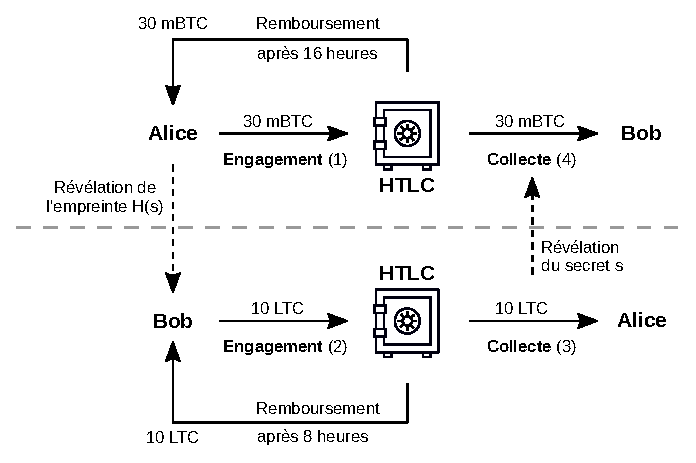
\includegraphics[scale=0.9]{img/atomic-swap-contract.eps}
  \caption{Contrats et transactions dans un échange atomique.}
  \label{fig:atomic-swap-contract}
\end{figure}

% Apport
Ce modèle garantit qu'aucun des deux participants ne peut se rembourser avant la fin du temps de verrouillage de Bob (8 heures)~; qu'Alice ne peut pas faire valoir sa transaction de remboursement au moment de la diffusion de sa transaction de collecte~; et que Bob ne peut pas s'approprier des fonds d'Alice tant qu'elle n'a pas diffusé sa transaction de collecte. Ces garanties rendent le procédé logiquement sécurisé, même si certains évènements perturbateurs peuvent survenir comme une augmentation des temps de confirmation liée à la volatilité du marché des frais.

% Historique et mise en œuvre
Le premier \eng{atomic swap} réel a été réalisé entre Litecoin et Decred le 19 septembre 2017 par Charlie Lee et Alex Yocom-Piatt\sendnote{Les adresses des contrats sur LTC et DCR étaient (respectivement) \longstring{MLp49daA411aoZ1TmGEdyLuTCE9YA6xhpc} et \longstring{DccPF1yt9cV8vhr97fq3umBx7RqV53MYGDY}. L'échange était de 1,337 LTC contre 2,4066 DCR. -- \eng{Decred-compatible cross-chain atomic swapping}, 20 septembre 2017~: \url{https://github.com/decred/atomicswap/blob/master/README.md\#first-mainnet-dcr-ltc-atomic-swap}.}. Aujourd'hui, les échanges atomiques sont rares, les carnets d'ordres de plateformes spécialisées comme AtomicDEX étant très peu fournis. Toutefois, avec le durcissement réglementaire sévissant dans l'écosystème et rendant les plateformes centralisées moins fiables, il n'est pas exclus qu'ils jouent un rôle majeur à l'avenir.

\section*{Les canaux de paiement}
\addcontentsline{toc}{section}{Les canaux de paiement}

% Canaux, définition, Lightning
Un cas particulier de l'application des contrats autonomes dans Bitcoin est le déploiement de canaux de paiement. Un canal de paiement est une manière pour deux utilisateurs d'effectuer des paiements répétés en bitcoins de manière sûre et instantanée sans publier de transactions sur la chaîne de blocs à partir de liquidités préalablement bloquées. Ces canaux sont notamment à la base du réseau Lightning, construit en surcouche de la chaîne.

% --- Canaux de paiement de Poon-Dryja ---

\subsection{Les canaux de paiement de Poon-Dryja} Même si l'idée d'un canal de paiement était envisagée dès les origines\pagenote{«~l'idée d'un canal de paiement était envisagée dès les origines~»~: Satoshi Nakamoto, \eng{Re: Open sourced my Java SPV impl}, \wtime{09/03/2011 16:15 UTC}~: \url{https://plan99.net/~mike/satoshi-emails/thread4.html}~; hashcoin, \eng{Instant TX for established business relationships (need replacements/nLockTime)}, \wtime{04/07/2011 02:16:23 UTC}~: \url{https://bitcointalk.org/index.php?topic=25786.msg320931\#msg320931}~;
Meni Rosenfeld, \eng{Trustless, instant, off-the-chain Bitcoin payments}, \wtime{05/07/2012 13:37:19 UTC}~: \url{https://bitcointalk.org/index.php?topic=91732.msg1010405\#msg1010405}~; Jeremy Spliman, \eng{[Bitcoin-development] Anti DoS for tx replacement}, \wtime{20/04/2013 01:48:11 UTC}~: \url{https://lists.linuxfoundation.org/pipermail/bitcoin-dev/2013-April/002433.html}~; Alex Akselrod, \eng{Bitcoin Wiki: Draft}, 12 mars 2013, \url{https://en.bitcoin.it/wiki/User:Aakselrod/Draft}~; Christian Decker, Roger Wattenhofer, \eng{A Fast and Scalable Payment Network with Bitcoin Duplex Micropayment Channels}, août 2015~: \url{https://www.researchgate.net/publication/277991245_A_Fast_and_Scalable_Payment_Network_with_Bitcoin_Duplex_Micropayment_Channels}.}, elle ne s'est concrétisée qu'avec le concept élaboré par Joseph Poon et Thaddeus Dryja dans le cadre de leur projet du réseau Lightning\sendnote{Joseph Poon et Thaddeus Dryja, \eng{The Bitcoin Lightning Network DRAFT Version 0.5}, 28 février 2015~: \url{https://lightning.network/lightning-network-paper-DRAFT-0.5.pdf}.}. Il s'agit d'un concept de canal bidirectionnel dont la sécurité repose sur un mécanisme de punition. Les deux participants bloquent des fonds dans un contrat et peuvent procéder à des paiements l'un vers l'autre dans la limite des liquidités disponibles. La somme des deux soldes des participants est appelée la capacité du canal.

% Trois phases : ouverture, négociation, fermeture
Un canal traverse trois phases au cours de son existence~:

\begin{itemize}
\item La phase d'ouverture ou d'installation, lors de laquelle les fonds sont bloqués par les participants sur un contrat autonome de multisignature 2-parmi-2~;
\item La phase de négociation ou de mise à jour, durant laquelle la répartition des fonds au sein du canal est ajustée~;
\item La phase de fermeture ou de règlement, au cours de laquelle les fonds sont distribués aux participants sur la chaîne, généralement de manière coopérative selon le dernier état du canal.
\end{itemize}

% to_local Output
%
% IF
%     <revocationpubkey>
% ELSE
%     <to_self_delay> CHECKSEQUENCEVERIFY DROP
%     <local_delayedpubkey>
% ENDIF
% CHECKSIG
%
% to_remote Output (with option_anchors)
%
% <remotepubkey> OP_CHECKSIGVERIFY 1 OP_CHECKSEQUENCEVERIFY

% Transactions d'engagement
La répartition initiale et la mise à jour du canal se font par l'intermédiaire de transactions d'engagement qui sont échangées entre les participants et \emph{qui ne sont pas diffusées} sur le réseau, sauf dans le cas d'un litige, c'est-à-dire d'une fermeture non coopérative. Ces transactions d'engagement sont asymétriques, dans le sens où les participants en possèdent chacun leur propre version.

% Répartition des fonds et contrat de réclamation
Supposons qu'Alice et Bob possèdent un canal, tel qu'illustré sur la figure~\ref{fig:poon-dryja-contracts}. Dans ce cas, la dernière transaction d'engagement d'Alice, qui peut uniquement être finalisée et diffusée par Bob, prend en compte l'état actualisé du canal et répartit les fonds entre l'adresse d'Alice et un contrat de réclamation. Ce contrat de réclamation contient deux clauses~:

\begin{itemize}
\item La récupération des fonds par Bob au terme d'un temps de verrouillage, ce qui répartit les fonds selon les soldes indiqués dans le canal~;
\item La récupération des fonds par Alice à l'aide d'une clé de révocation qui est révélée plus tard lorsque le canal est de nouveau mis à jour.
\end{itemize}

% Actualisation suite à un paiement
Si un paiement a lieu d'Alice vers Bob, la mise à jour du canal se fait de la manière suivante. Alice construit et signe sa transaction d'engagement en utilisant la clé publique de révocation de Bob que ce dernier lui a transmise au préalable. Seul Bob peut finaliser la signature de cette transaction et la diffuser sur le réseau. Bob lui répond en lui envoyant sa clé privée de révocation, ce qui rend la dernière transaction d'engagement d'Alice inopérante. La même chose se produit ensuite de manière symétrique~: Bob construit et signe sa transaction d'engagement qu'il transmet à Alice, et cette dernière lui révèle en échange sa clé privée de révocation, ce qui rend la transaction d'engagement de Bob impuissante\sendnote{Andreas M. Antonopoulos, Olaoluwa Osuntokun, René Pickhardt, «~Payment Channels~», in \eng{Mastering the Lightning Network: A Second Layer Blockchain Protocol for Instant Bitcoin Payments}, O'Reilly Media, 2022, pp. 149--184.}.

% Mécanisme de punition
La révélation de la clé de révocation à chaque étape de mise à jour rend possible l'activation d'un mécanisme de punition à tout moment. Si l'une des deux parties diffuse une transaction d'engagement correspondant à un état antérieur du canal, alors l'autre peut récupérer \emph{l'intégralité} des fonds du canal. Par exemple, Alice pourrait récupérer les fonds de Bob si ce dernier était amené à diffuser le précédent état du canal dans le but d'«~annuler~» le dernier paiement réalisé.

\begin{figure}[ht]
  \centering
  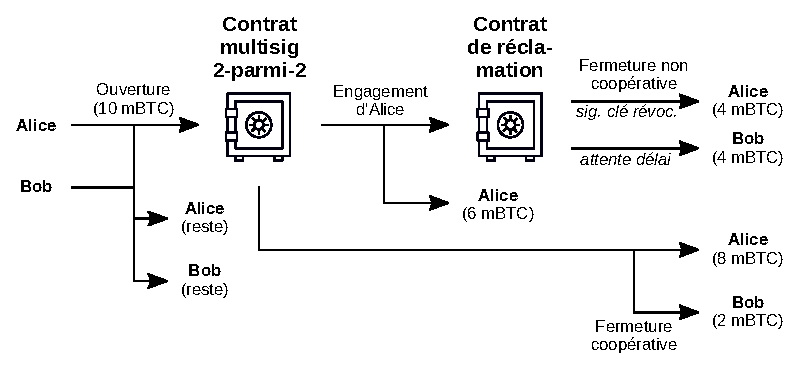
\includegraphics[scale=0.8]{img/lightning-poon-dryja-channel-contracts.eps}
  \caption{Contrats et transactions dans un canal de paiement de Poon-Dryja~: cas d'un paiement de Bob de 2~mBTC à Alice.}
  \label{fig:poon-dryja-contracts}
\end{figure}

% Défaut du mécanisme de punition
Le défaut principal de ce mécanisme de punition est qu'il faut surveiller le réseau en permanence pour éviter un vol, ce qui se fait avec un nœud complet ou bien avec un tiers de confiance bien choisi («~tour de garde~» ou «~\eng{watchtower}~»).

% Défauts dûs au mécanisme de punition
Ce fonctionnement des canaux de Poon-Dryja fait aussi que toute erreur est très pénalisante~: la diffusion accidentelle d'une transaction d'engagement antérieure mène à la récupération des fonds par l'autre partie. Il a également d'autres défauts~: il impose de conserver l'ensemble des états antérieurs du canal, il oblige les participants à choisir les frais des transactions à l'avance et il alourdit considérablement les innovations au sein du réseau Lightning. C'est par volonté d'améliorer cette situation qu'ont été conceptualisés les canaux dits «~de Decker-Russell-Osuntokun~».

% --- Canaux de paiement de Decker-Russell-Osuntokun ---

\subsection{Les canaux de paiement de Decker-Russell-Osuntokun} Les canaux de paiement de Decker-Russell-Osuntokun ont été décrits par Christian Decker, Rusty Russell et Olaoluwa Osuntokun dans un livre blanc publié en avril 2018\sendnote{Christian Decker, Rusty Russell, Olaoluwa Osuntokun, \eng{eltoo: A Simple Layer2 Protocol for Bitcoin}, 30 avril 2018~: \url{https://blockstream.com/eltoo.pdf}.}. Le protocole sous-jacent est appelé Eltoo, qui est une déformation de l'anglais «~\eng{L2}~» (signifiant \eng{layer two}).

% Fonctionnement
Le fonctionnement des canaux de Decker-Russel-Osuntokun se base sur une chaîne de transactions, qui ne sont pas censées être diffusées sur la chaîne, sauf celles d'ouverture et de fermeture (cf. figure~\ref{fig:eltoo}). Le principe est le suivant~:

\begin{itemize}
\item Le canal est ouvert par une transaction d'ouverture ($T_{u,0}$), préalablement garantie par une transaction de règlement ($T_{s,0}$) qui rembourse les participants en cas de litige~;
\item Le canal est mis à jour par des transactions de mise à jour ($T_{u,i}$) qui invalident les transactions de règlement précédentes ($T_{s,i-1}$)~;
\item La fermeture du canal peut se faire après un certain délai d'expiration par la diffusion de la dernière transaction de règlement ($T_{s,i}$).
\end{itemize}

Ici il n'y a plus besoin de recourir à des clés de révocation pour rendre les anciens états du canal inexploitables~: ce sont les transactions elles-mêmes qui ont ce rôle. Eltoo fait intervenir ce qu'on appelle des transactions flottantes, qui peuvent dépenser les fonds issus de n'importe quelle transaction de mise à jour précédente. De cette manière, chaque transaction de mise à jour est flottante, ainsi que chaque transaction de règlement, ce qui permet d'omettre toutes les mises à jour précédentes. De plus, un numéro d'état est inscrit dans chaque transaction pour ordonner les transactions et ainsi éviter la diffusion d'un état antérieur. % un numéro d'état est inscrit dans chaque transaction grâce à une utilisation astucieuse du code opération OP\_CHECKLOCKTIMEVERIFY

\begin{figure}[h]
  \centering
  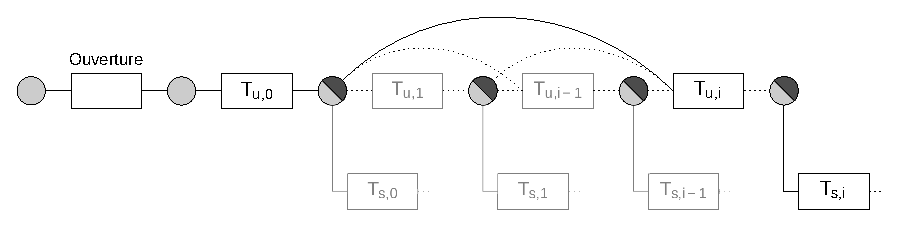
\includegraphics[scale=0.7]{img/eltoo-offchain-protocol.eps}
  \caption{Aperçu du protocole Eltoo.}
  \label{fig:eltoo}
\end{figure}

Une transaction supplémentaire est ajoutée à la chaîne de transactions pour éviter que le délai d'expiration des transactions de règlement $T_{s,i}$ soit atteint et qu'elles soient diffusées sur la chaîne. Cette transaction envoie simplement les fonds vers un compte multisignatures classique, et est signée et diffusée après la signature des premières transactions de mise à jour et de règlement ($T_{u,0}$ et $T_{s,0}$). Le délai d'expiration ne commence que lorsque la transaction $T_{u,0}$ est diffusée.

Ce fonctionnement permet d'obtenir un protocole simple de mise à jour du canal, peu contraignant pour les nœuds, sans mécanisme de punition, et permettant de ne pas à avoir à décider les frais à l'avance. Cette facilité d'implémentation pourrait rendre plus aisée la création de contrats plus complexes sur Lightning, comme les canaux de paiement à 3 participants ou plus. En outre, leur implémentation ne doit en aucun cas remplacer celle des canaux de Poon-Dryja~: les deux modèles peuvent coexister au sein d'un seul et même réseau de canaux de paiement.

Les transactions flottantes sont implémentées à l'aide de \longstring{SIGHASH\_ANYPREVOUT}. La mise en œuvre de Eltoo repose donc sur l'intégration du BIP-118 dans Bitcoin.

\section*{L'inscription de données arbitraires}
\addcontentsline{toc}{section}{L'inscription de données arbitraires}

% Données arbitraire
Bitcoin permet d'inscrire des données non financières sur la chaîne, c'est-à-dire des données qui ne sont pas nécessaires dans le blocage et le déblocage des fonds et qui sont interprétées de manière extérieure au protocole. Même en imposant toutes les restrictions possibles, on ne peut pas empêcher l'inscription de ces données, même s'il est possible de la rendre plus coûteuse.

% Laisser sa marque pour la postérité
La chaîne de blocs de la version principale de Bitcoin est largement partagée autour du monde, et sera conservée par l'humanité, au moins comme un reliquat historique, laissant supposer que ce qui y est stocké sera conservé très longtemps. Cette caractéristique pousse les gens à y inclure des choses qui leur tiennent à cœur. Il est dans la nature de l'homme de chercher à laisser des traces de son passage sur Terre et écrire sur un registre réputé immuable est une manière de le faire.

% Méthodes d'inscription
Il existe diverses méthodes d'inscription, qui ont chacune leurs qualités et leurs défauts\pagenote{«~diverses méthodes d'inscription~»~: Andrew Sward, Ivy Vecna, Forrest Stonedahl, \eng{Data Insertion in Bitcoin's Blockchain}, in \eng{Ledger}, vol. 3, avril 2018~: \url{https://doi.org/10.5195/ledger.2018.101}.}. Celles-ci ont évolué au fur et à mesure des années, alors que cette utilisation se libéralisait.

% Inscription dans la transaction de récompense par les mineurs
D'une part, l'écriture de données arbitraires peut être réalisée par les mineurs au sein de l'entrée de transaction de récompense, et plus précisément dans le script de déverrouillage. Ce champ est en effet superflu conceptuellement, la base de pièce ne faisant référence à aucune sortie existante, et peut donc être exploité de manière discrétionnaire. C'est cette méthode dont Satoshi Nakamoto a fait usage pour inscrire le désormais célèbre titre de une du Times du 3 janvier 2009 dans le bloc de genèse~:

\begin{quote}
\eng{The Times 03/Jan/2009 Chancellor on brink of second bailout for banks}
\end{quote}

% Inscriptions par les mineurs
D'autres blocs contiennent des messages emblématiques. Le bloc d'exode de BCH (de hauteur 478~559) contenait un message de bienvenue pour Shuya Yang, la fille du PDG de la coopérative ViaBTC\pagenote{«~message de bienvenue pour Shuya Yang~»~: \eng{Welcome to the world, Shuya Yang!}, \url{https://blockchair.com/bitcoin-cash/block/478559}.}. Le bloc précédant le troisième halving sur BTC en 2020 (de hauteur 629~999) incluait le titre d'un article du New York Times du 9 avril annonçant l'injection de liquidité record de la Réserve Fédérale (2~300 milliars de dollars) en réaction à la crise du Covid-19~: «~\eng{NYTimes 09/Apr/2020 With \$2.3T Injection, Fed's Plan Far Exceeds 2008 Rescue}~».\pagenote{«~Le bloc précédant le troisième halving sur BTC en 2020 [...] incluait le titre d'un article du New York Times~»~: \url{https://blockchair.com/bitcoin/block/629999}.}

Le script de déverrouillage de la base de pièce peut être utilisé pour écrire d'autres données. C'est le cas du nonce supplémentaire (le critère qui a permis d'identifier les bitcoins de Satoshi\pagenote{«~le critère qui a permis d'identifier les bitcoins de Satoshi~»~: Sergio Lerner, \eng{The Well Deserved Fortune of Satoshi Nakamoto, Bitcoin creator, Visionary and Genius}, 17 avril 2013~: \url{https://bitslog.com/2013/04/17/the-well-deserved-fortune-of-satoshi-nakamoto/}.}). C'est aussi le cas du signalement des coopératives minières qui est réalisé \emph{via} ce champ~: par exemple, la base de pièce du bloc 751~005 contient la chaîne de caractères \longstring{poolin.com}, ce qui indique que sa validation a probablement été réalisée par la coopérative chinoise Poolin.

% Inscription par les utilisateurs
D'autre part, l'inscription des données arbitraires peut aussi être le fait des utilisateurs, qui peuvent les inclure dans leurs transactions et payer les frais correspondants. Plusieurs méthodes ont été exploitées pour ce faire.

% Stockage dans les sorties transactionnelles (P2PKH, P2MS et P2SH)
Avant 2014, on procédait la plupart du temps à ces inscriptions en stockant les données dans les scripts de verrouillage, par exemple par l'utilisation de l'instruction de dépilement \texttt{OP\_DROP}\sendnote{La transaction \longstring{c0b2cf75b47d1e7f48cdb4287109ff1dd5bcf146d5f77a9e8784c0c9c0ef02ad}, confirmée le 13 décembre 2012, contient par exemple la chaîne de caractères \longstring{TheCakeIsALie\textbackslash{}n} en référence au jeu vidéo Portal.}. Une autre pratique courante était d'inscrire les données dans les sorties de type P2PKH, qui étaient rendues indépensables au passage. Cette méthode était extrêmement coûteuse en raison de la forme de la transaction (imposant l'inscription dans les sorties transactionnelles) et le fait de devoir envoyer des montants non nuls en sortie. Elle était également dommageable pour le système dans son ensemble, car elle encombrait l'ensemble des UTXO.

% Stockage dans les sorties NULLDATA (première utilisation en mars 2013 : 1a2e22a717d626fc5db363582007c46924ae6b28319f07cb1b907776bd8293fc, standardisation en mars 2014 : v0.9.0)
Après 2014, une manière plus efficace de stocker des données a été autorisée par le biais de la standardisation du schéma NULLDATA qui se basait sur l'instruction \texttt{OP\_RETURN}. Ce changement permettait de créer «~une sortie assurément élagable, pour éviter les schémas de stockage d'informations [...] qui enregistraient des données arbitraires, telles que des images, en tant que sorties transactionnelles éternellement indépensables, gonflant ainsi la base de données des UTXO de bitcoin\sendnote{Bitcoin Core, \eng{Bitcoin Core version 0.9.0 released}, 19 mars 2014~: \url{https://bitcoin.org/en/release/v0.9.0\#opreturn-and-data-in-the-block-chain}.}~». Il limitait aussi le gaspillage de fonds en autorisant la création d'une sortie de 0 satoshi. Ce schéma s'est rapidement imposé comme la manière la plus populaire pour publier des informations sur la chaîne. % "The OP_RETURN change creates a provably-prunable output, to avoid data storage schemes – some of which were already deployed – that were storing arbitrary data such as images as forever-unspendable TX outputs, bloating bitcoin's UTXO database."

% Stockage dans les entrées transactionnelles : P2SH, P2WPKH, P2WSH, P2TR
En outre, il est aussi possible de stocker des données au sein des entrées transactionnelles ou des témoins liés, lors de la dépense de sorties P2SH, P2WSH ou P2TR. Cette écriture peut se faire dans les scripts de récupération ou bien dans les éléments de déverrouillage. Cette méthode a l'avantage de ne pas surcharger l'ensemble des UTXO. Côté utilisateur, dans les entrées où SegWit s'applique, elle a pour bénéfice de diviser le coût des données arbitraires inscrites dans la transactions par quatre.

% --- Inscriptions ---

Ces différentes méthodes ont été utilisées pour inscrire toutes sortes de choses sur la chaîne, dont notamment des empreintes cryptographiques, du texte et des images\sendnote{Ken Shirriff, \eng{Hidden surprises in the Bitcoin blockchain and how they are stored: Nelson Mandela, Wikileaks, photos, and Python software}, 16 février 2014~: \url{https://www.righto.com/2014/02/ascii-bernanke-wikileaks-photographs.html}.}.

% Horodatage par inscription d'empreintes
D'abord, on peut inscrire une empreinte, l'inscription servant alors à l'horodatage. Il s'agit d'inscrire l'empreinte d'un fichier sur la chaîne en tant que preuve d'existence. Cette idée a été mise en avant en février 2009 par Hal Finney dans un de ses courriels adressés à la liste de diffusion dédiée à Bitcoin. Il suggérait alors que «~la pile de blocs de bitcoin serait parfaite~» pour «~prouver qu'un certain document a existé à un certain moment dans le passé\sendnote{Hal Finney, \eng{Re: [bitcoin-list] Bitcoin v0.1.5 released}, \wtime{27/02/2009 20:00:12 UTC}, archive~: \url{https://web.archive.org/web/20131016004925/http://sourceforge.net/p/bitcoin/mailman/bitcoin-list/?viewmonth=200902}.}~», un point de vue approuvé par Satoshi\pagenote{«~un point de vue approuvé par Satoshi~»~: Satoshi Nakamoto, \eng{Re: [bitcoin-list] Bitcoin v0.1.5 released}, \wtime{04/03/2009 16:59:12 UTC}, archive~: \url{https://web.archive.org/web/20131016004648/http://sourceforge.net/p/bitcoin/mailman/bitcoin-list/?viewmonth=200903}~: «~En effet, Bitcoin est un serveur d'horodatage sécurisé et distribué pour les transactions. Quelques lignes de code pourraient créer une transaction avec une empreinte supplémentaire de tout ce qui doit être horodaté. Je devrais ajouter une commande pour horodater un fichier de cette façon.~»}. En somme, cette pratique permet de démontrer la connaissance d'une information avant sa publication, et donc indirectement qu'on en est l'auteur probable. Ce type d'usage a notamment été mis en œuvre par l'entreprise française Woleet. % "BTW I don't remember if we talked about this, but the other day some people were mentioning secure timestamping. You want to be able to prove that a certain document existed at a certain time in the past. Seems to me that bitcoin's stack of blocks would be perfect for this." -- "Indeed, Bitcoin is a distributed secure timestamp server for transactions.  A few lines of code could create a transaction with an extra hash in it of anything that needs to be timestamped. I should add a command to timestamp a file that way."

% Empreintes pour IPFS
Cette possibilité peut aussi être exploité par les systèmes décentralisés d'hébergement de fichiers, comme le système IPFS (InterPlanetary File System) qui utiliser les empreintes des fichiers pour les identifier et permettre leur stockage par un réseau pair à pair d'utilisateurs. Il est donc possible d'associer le texte écrit sur la chaîne de blocs et des images ou des vidéos, hébergées de manière décentralisée.

% Texte
Ensuite, on peut inscrire un texte, qui est généralement encodé en ASCII~/~UTF-8. Par exemple, la phrase «~La beauté sauvera le monde.~» a été inscrite sur la chaîne de BTC le 10 août 2022 dans la transaction d'identifiant \longstring{08e5ce0783ab6d5534e234136df02e0e240f76108eb6af04b8b624646b66f5eb}. L'inscription de textes permet aussi de dessiner des images en art ASCII. C'est le cas de l'hommage à Len Sassaman (voir figure~\ref{fig:sassaman-tribute}), décédé en juillet 2011, qui a été inscrit sur la chaîne par les développeurs Dan Kaminsky et Travis Goodspeed dans des sorties P2PKH, et qui contient notamment une représentation de l'ancien président de la Fed, Ben Bernanke\pagenote{«~l'hommage à Len Sassaman [...] inscrit sur la chaîne par les développeurs Dan Kaminsky et Travis Goodspeed~»~: Cet hommage peut être retrouvé dans la transaction d'identifiant \longstring{930a2114cdaa86e1fac46d15c74e81c09eee1d4150ff9d48e76cb0697d8e1d72} confirmée le 30 juillet 2011.}.

\begin{figure}[h]
  \begin{Verbatim}[fontsize=\footnotesize]
        ---BEGIN TRIBUTE---  =-=-=-=-=-=-=-=-=-=     ASCII BERNANKE
        #./BitLen            LEN "rabbi" SASSAMA  :'::.:::::.:::.::.:
        :::::::::::::::::::       1980-2011       : :.: ' ' ' ' : :':
        :::::::.::.::.:.:::  Len was our friend.  :.:     _.__    '.:
        :.: :.' ' ' ' ' : :  A brilliant mind,    :   _,^"   "^x,   :
        :.:'' ,,xiW,"4x, ''  a kind soul, and     '  x7'        `4,
        :  ,dWWWXXXXi,4WX,   a devious schemer;    XX7            4XX
        ' dWWWXXX7"     `X,  husband to Meredith   XX              XX
         lWWWXX7   __   _ X  brother to Calvin,    Xl ,xxx,   ,xxx,XX
        :WWWXX7 ,xXX7' "^^X  son to Jim and       ( ' _,+o, | ,o+,"
        lWWWX7, _.+,, _.+.,  Dana Hartshorn,       4   "-^' X "^-'" 7
        :WWW7,. `^"-" ,^-'   coauthor and          l,     ( ))     ,X
         WW",X:        X,    cofounder and         :Xx,_ ,xXXXxx,_,XX
         "7^^Xl.    _(_x7'   Shmoo and so much      4XXiX'-___-`XXXX'
         l ( :X:       __ _  more.  We dedicate      4XXi,_   _iXX7'
         `. " XX  ,xxWWWWX7  this silly hack to     , `4XXXXXXXXX^ _,
          )X- "" 4X" .___.   Len, who would have    Xx,  ""^^^XX7,xX
        ,W X     :Xi  _,,_   found it absolutely  W,"4WWx,_ _,XxWWX7'
        WW X      4XiyXWWXd  hilarious.           Xwi, "4WW7""4WW7',W
        "" ,,      4XWWWWXX  --Dan Kaminsky,      TXXWw, ^7 Xk 47 ,WH
        , R7X,       "^447^  Travis Goodspeed     :TXXXWw,_ "), ,wWT:
        R, "4RXk,      _, ,  P.S.  My apologies,  ::TTXXWWW lXl WWT:
        TWk  "4RXXi,   X',x  BitCoin people.  He  ----END TRIBUTE----
        lTWk,  "4RRR7' 4 XH  also would have
        :lWWWk,  ^"     `4   LOL'd at BitCoin's
        ::TTXWWi,_  Xll :..  new dependency upon
  \end{Verbatim}
  \caption{Hommage à Len Sassaman (art ASCII).}
  \label{fig:sassaman-tribute}
\end{figure}

% Images
Enfin, on peut inclure une image, qui peut être encodée dans de multiples formats, dont notamment en JPEG ou en PNG. Un logo Bitcoin inscrit le 13 mai 2011 peut par exemple être retrouvé\pagenote{«~Un logo Bitcoin inscrit le 13 mai 2011 peut par exemple être retrouvé~»~: Transactions \longstring{ceb1a7fb57ef8b75ac59b56dd859d5cb3ab5c31168aa55eb3819cd5ddbd3d806} et \longstring{9173744691ac25f3cd94f35d4fc0e0a2b9d1ab17b4fe562acc07660552f95518}}. Un hommage à Nelson Mandela accompagné d'une photo a été publié le 7 décembre 2013, quelques jours après sa mort\pagenote{«~Un hommage à Nelson Mandela accompagné d'une photo a été publié le 7 décembre 2013, quelques jours après sa mort~»~: Voir transaction \longstring{8881a937a437ff6ce83be3a89d77ea88ee12315f37f7ef0dd3742c30eef92dba}.}. En 2022, l'absence de restriction standarde sur la taille des scripts de Taproot a permis de réaliser des inscriptions volumineuses d'une manière bien plus transparente et directe. C'est ce qui a notamment permis d'inscrire l'image des Taproot Wizards qui pesait quasiment 4~Mo (voir figure~\ref{fig:taproot-wizards}).

\begin{figure}[h]
  \centering
  
\includegraphics[scale=0.6]{img/taproot-wizards-small-0301e0480b374b32851a9462db29dc19fe830a7f7d7a88b81612b9d42099c0aei0.jpg}
  \caption{Image (réduite) des Taproot Wizards.}
  \label{fig:taproot-wizards}
\end{figure}

% Autres fichiers, pertinence de cet usage
De manière générale, tout format de fichier peut être stocké sur la chaîne au moyen de transactions multiples~: un document\pagenote{«~un document~»~: Le PDF du livre blanc de Bitcoin a été inscrit sous forme de sorties P2MS au sein de la transaction \longstring{54e48e5f5c656b26c3bca14a8c95aa583d07ebe84dde3b7dd4a78f4e4186e713}, le 6 avril 2013.}, un livre, une vidéo, un jeu\pagenote{«~un jeu~»~: Nicholas Carlini, \eng{Yet Another Doom Clone}, 1\ier{} février 2023~: \url{https://ordinals.com/inscription/521f8eccffa4c41a3a7728dd012ea5a4a02feed81f41159231251ecf1e5c79dai0}, \url{https://nicholas.carlini.com/writing/2019/javascript-doom-clone-game.html}.}, etc. Cependant, cette utilisation n'est pas forcément toujours pertinente. L'inscription demande le paiement de frais, parfois élevés, et la chaîne de blocs de BTC n'est pas franchement faite pour conserver des données volumineuses. La publication de ces fichiers sur IPFS et sur serveur local est généralement bien plus opportune.

% Bitcoin SV
Notons que la communauté de Bitcoin SV s'est focalisée sur le stockage de données, considérant que son registre était une «~source universelle de vérité\sendnote{CoinGeek, \eng{Jerry Chan: Bitcoin's value is as a universal source of truth}, 17 juillet 2019~: \url{https://coingeek.com/jerry-chan-bitcoins-value-is-as-a-universal-source-of-truth-video/}.}~». On peut ainsi retrouver un volume assez importants de données météorologiques sur sa chaîne, qui y sont inscrites depuis 2019\pagenote{«~données météorologiques~»~: Helen Partz, \eng{98\% of BSV Transactions Used for Writing Weather Data on Blockchain: Report}, 24 juin 2019~: \url{https://cointelegraph.com/news/98-of-bsv-transactions-used-for-writing-weather-data-on-blockchain-report}.}. Cela fait que le réseau BSV est extrêmement centralisé tant du point de vue minier que commercial, ce qui remet en cause l'utilité première de l'inscription d'informations sur une chaîne de blocs~: l'immuabilité.

\section*{Les métaprotocoles}
\addcontentsline{toc}{section}{Les métaprotocoles}

% Définition
Les métaprotocoles sont des protocoles qui se servent du protocole de base pour fonctionner. Ils font usage de l'inscription de données arbitraires sur la chaîne pour inclure des instructions qui sont interprétées par des implémentations logicielles spécifiques\pagenote{«~Ils font usage de l'inscription de données arbitraires sur la chaîne pour inclure des instructions qui sont interprétées par des implémentations logicielles spécifiques~»~: C'est en ce sens que les métaprotocoles peuvent être appelés des surcouches, même si on préfère généralement utiliser ce terme pour parler des systèmes comme Lightning par exemple.}. Ils ont pour particularité d'être plus extensifs que le protocole de base.

% Bitcoin 2.0
Il ne s'agit pas d'une idée nouvelle. Dès les premières années d'existence de Bitcoin, certaines personnes ont souhaité l'exploiter plus en profondeur, en se servant de lui d'une autre manière que comme un instrument de transfert de valeur. Ce mouvement initial, visant à ajouter des fonctionnalités à Bitcoin de cette façon, était appelé «~Bitcoin 2.0~». Il a finalement mené à l'élaboration d'Ethereum à partir de 2013.

% Colored Coins (2012)
Le premier type de métaprotocole qui a été élaboré est le procédé des \eng{colored coins}, ou pièces colorées en français, qui consiste à marquer des pièces (UTXO) par l'inscription annexe de données, comme montré sur la figure~\ref{fig:colored-coin}. Chaque type de jeton créé est lié à un identifiant, que l'on peut assimiler à une couleur, d'où le nom de ce procédé. L'idée a été présentée en 2012 par Yoni Assia et Meni Rosenfeld\sendnote{Yoni Assia, \eng{bitcoin 2.X (aka Colored Bitcoin) – initial specs}, 27 mars 2012~: \url{https://yoniassia.com/coloredbitcoin/}~; Meni Rosenfeld, \eng{Overview of Colored Coins}, 4 décembre 2012~: \url{https://bitcoil.co.il/BitcoinX.pdf}.}. % inscrites notamment par l'utilisation de l'opérateur \texttt{OP\_RETURN}

\begin{figure}[h]
  \centering
  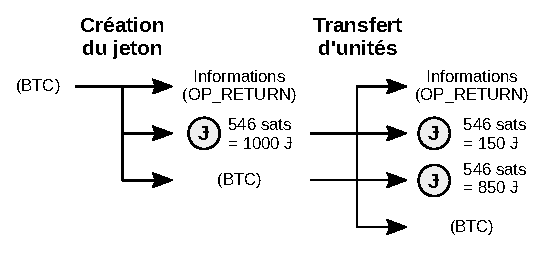
\includegraphics[scale=1]{img/colored-coin.eps}
  \caption{Création et transfert d'un jeton émis sous la forme d'un colored coin.}
  \label{fig:colored-coin}
\end{figure}

\vspace{-1em}
% Implémentation des colored coins
L'implémentation de ce concept a été réalisée dès la fin de l'année 2012 par l'intermédiaire du ChromaWallet\pagenote{«~ChromaWallet~»~: Alex Mizrahi, \eng{ChromaWallet (colored coins): issue and trade private currencies/stocks/bonds/..}, \wtime{07/09/2012 12:46:12 UTC}~: \url{https://bitcointalk.org/index.php?topic=106373.msg1167516\#msg1167516}.}. Cependant, elle n'a vraiment pris de l'ampleur qu'à partir de 2014, avec l'apparition des Open Assets de Coinprism, des \eng{CoinSpark assets} de Coin Sciences, et des Colored Coins de Colu. Ces usages sont depuis tombés en désuétude, même si le procédé a pu servir de manière sporadique au fil des années, comme dans le cas du jeton BSQ de Bisq créé en 2018 comme base de sa DAO. Une tentative de restauration a également été faite sur Bitcoin Cash avec les jetons SLP, sans grand succès. % Open Assets (\texttt{OA}), Colored Coins (\texttt{CC}), CoinSpark assets (\texttt{SPK})

% Mastercoin et Counterparty
Au-delà des pièces colorées, il existait des protocoles plus évolués qui avaient la particularité de gérer une unité de compte propre. Il s'agissait essentiellement de Mastercoin, qui a été renommé en Omni en mars 2015, et de Counterparty.

% Mastercoin (2013)
Le premier métaprotocole avancé a été Mastercoin\pagenote{«~Mastercoin~»~: Le mot \eng{master} dans le nom de Mastercoin est l'acronyme de «~\eng{Metadata Archival by Standard Transaction Embedding Records}~», d'après les spécifications techniques~: \url{https://github.com/OmniLayer/spec/blob/master/OmniSpecification-v0.6.adoc}.}, dont le livre blanc, intitulé «~\eng{The Second Bitcoin Whitepaper}~», a été publié le 6 janvier 2012 par J.R. Willett\sendnote{J.R. Willett, \eng{The Second Bitcoin Whitepaper}, 6 janvier 2012, archive~: \url{https://cryptochainuni.com/wp-content/uploads/Mastercoin-2nd-Bitcoin-Whitepaper.pdf}.}\pagenote{«~«~le livre blanc, intitulé "\eng{The Second Bitcoin Whitepaper}", a été publié le 6 janvier 2012 par J.R. Willett~»~: J.R. Willett, \eng{[It's here] The Second Bitcoin Whitepaper}, \wtime{06/01/2012 22:42:24 UTC}~: \url{https://bitcointalk.org/index.php?topic=56901.msg678427\#msg678427}.}. Il s'agissait d'un protocole permettant à ses utilisateurs de créer leurs propres devises, appelées «~\eng{user currencies}~». Mastercoin reposait sur une unité de compte notée le MSC, qui a fait l'objet d'une prévente d'un mois en juillet-août 2013\sendnote{Tous les bitcoins envoyés à l'adresse \longstring{1EXoDusjGwvnjZUyKkxZ4UHEf77z6A5S4P} étaient transformés en MSC à raison de 100~MSC au début, taux dégressif au fil des semaines. }. C'était la première \eng{Initial Coin Offering} de l'histoire, et elle a recueilli 5~120~BTC, soit plus de 500~000~\$ à ce moment-là.

% USDT
Le plus grand succès de ce protocole a probablement été la création du premier stablecoin, le Tether USD, qui a été émis sous le nom de Realcoin en octobre 2014. Mastercoin~/~Omni a longtemps été l'unique manière de posséder et de transférer de l'USDT avant que le jeton ne soit émis massivement sur d'autres chaînes comme Ethereum et Tron.

% Counterparty (2014)
Le second métaprotocole avancé a été Counterparty, lancé en janvier 2014. Cette plateforme reposait également sur un jeton natif, le XCP, qui lui servait de carburant, et qui a été créé par brûlage de bitcoins durant son premier mois d'existence\sendnote{Tous les bitcoins envoyés à l'adresse \longstring{1CounterpartyXXXXXXXXXXXXXXXUWLpVr} entre le 2 janvier et le 3 février 2014 étaient convertis en XCP à un taux qui variait entre 1~000 et 1~500 XCP par BTC}. Ce sont 2~140 bitcoins qui ont ainsi été rendus inutilisables pour donner vie à plus de 2,6 millions de XCP, encore en circulation aujourd'hui. Counterparty se voulait plus flexible que Mastercoin en rendant possible l'implémentation de contrats autonomes, notamment dans le but de créer des jetons et d'héberger des plateformes d'échange décentralisées, appelées des «~distributeurs~».

% Jetons non fongibles (NFT)
En particulier, Counterparty a été la première plateforme à proposer la gestion de jetons non fongibles (NFT). Il s'agissait là de mettre en œuvre une vieille idée, qui avait notamment été mise en valeur par Hal Finney en 1993 sur la liste de diffusion cypherpunk sous la forme de «~cartes à collectionner cryptographiques\sendnote{Hal Finney, \eng{Crypto trading cards.}, \wtime{17/01/1993 18:48:02 UTC}~: \url{https://cypherpunks.venona.com/date/1993/01/msg00152.html}.}~». Counterparty a ainsi hébergé une multitude de collections de tels objets, comme les cartes à jouer de \eng{Spells of Genesis} et de SaruTobi créées en 2015, ou les Rare Pepes émis entre 2016 et 2018\pagenote{«~une multitude de collections de tels objets~»~: Vlad Costea, \eng{Bitcoin NFTs On Counterparty (And How To Get Or Create Your First One)}, 29 décembre 2021~: \url{https://bitcoin-takeover.com/bitcoin-nfts-on-counterparty-and-how-to-get-or-create-your-first-one/}.}.

% Memo (2018)
En 2018, l'apparition de Bitcoin Cash a motivé la création d'un média social dont les données seraient entièrement stockées sur la chaîne, les développeurs de BCH étant plus libéraux à ce sujet. Le protocole s'appelait Memo et consistait à publier de courts messages visibles publiquement sous un profil défini et à pouvoir suivre les autres utilisateurs, à aimer et répondre à leurs messages. L'idée était d'obtenir une sorte de réseau social résistant à la censure, mais souffrait néanmoins de la nécessité de payer des frais à chaque action. \pagenote{«~Le protocole s'appelait Memo et consistait à publier de courts messages visibles publiquement sous un profil défini et à pouvoir suivre les autres utilisateurs, à aimer et répondre à leurs messages~»~: \url{https://memo.cash/protocol}.}

% Ordinals (2023), BRC-20, STAMPS
Tous ces protocoles ont perdu leur attrait jusqu'à l'apparition du protocole Ordinals, lancé en janvier 2023. Ce métaprotocole permettait de créer et de gérer des «~artéfacts numériques~», c'est-à-dire des NFT dont l'intégralité des données est stockée de manière immuable sur une chaîne résistante à la censure. Le protocole Ordinals reposait sur une «~théorie des ordinaux~» permettant de suivre et de transférer des satoshis liés à une inscription, comme un texte, une image ou autre chose\pagenote{«~Le protocole Ordinals~»~: \url{https://docs.ordinals.com/}.}. En particulier, Ordinals a été utilisé pour émuler la propriété et le transfert de jetons fongibles, baptisés «~BRC-20~», dont le succès spéculatif a provoqué une congestion du réseau menant à une hausse des frais de transaction historique. Le succès d'Ordinals a également inspiré la création du protocole STAMPS, qui se basait sur Counterparty pour le suivi des artéfacts et stockait leurs données dans des sorties P2MS\pagenote{«~STAMPS~»~: STAMP est l'acronyme de \eng{Secure, Tradeable Art Maintained Permanently}. -- Mike In Space, \eng{STAMPS: A Protocol for Storing Images On-Chain in Transaction Outputs Immutably on Bitcoin}, 6 avril 2023~: \url{https://github.com/mikeinspace/stamps/tree/main}.}.

% Opposition
Toutes ces pratiques ont créé des débats. En effet, Bitcoin était présenté comme un modèle de monnaie numérique et il semblait contreproductif d'en faire un protocole de conservation de données qui ne seraient pas relatives au transfert de bitcoins. Ainsi, dès décembre 2010, Jeff Garzik s'opposait au fait d'utiliser la chaîne pour le stockage généralisé\sendnote{Jeff Garzik, \eng{Resist the urge to use block chain for generalized storage}, \wtime{07/12/2010 22:04:54 UTC}~: \url{https://bitcointalk.org/index.php?topic=2129.msg27884\#msg27884}.}. Plus tard, en 2014, des disputes similaires ont éclaté au sujet de Counterparty\sendnote{BitMEX Research, \eng{The OP\_Return Wars of 2014 – Dapps Vs Bitcoin Transactions}, 12 juillet 2022~: \url{https://blog.bitmex.com/dapps-or-only-bitcoin-transactions-the-2014-debate/}.}. En 2023, c'est également la même discorde qui a eu lieu suite au succès d'Ordinals\sendnote{pourteaux, \eng{Illegitimate bitcoin transactions}, 25 janvier 2023~: \url{https://read.pourteaux.xyz/p/illegitimate-bitcoin-transactions}.}.

% Premier défaut : manque de vérification
Ces métaprotocoles présentent deux défauts majeurs. Le premier est que la vérification de leurs règles dépend d'un petit sous-ensemble de nœuds du réseau. En effet, la gestion d'un tel protocole construit en surcouche demande des ressources supplémentaires, notamment en ce qui concerne l'indexation pour les pièces colorées. De ce fait, peu de personnes déploient une implémentation complète, ce qui centralise considérablement le protocole et le rend sensible à l'altération par un adversaire qui aurait pour but de le censurer.

% Second défaut : frais
Le second défaut concerne leurs frais d'utilisation parfois très élevés, surtout si la limite de capacité transactionnelle du réseau est atteinte. Les transactions qui mettent en place ces solutions sont nécessairement plus volumineuses que les transactions normales et entraînent par conséquent des frais plus élevés. Elles sont donc plus facilement exclues par l'augmentation des frais issue de la congestion du réseau.

% Conséquences de ces défauts
C'est pour ces raisons que les personnes qui ont travaillé sur ces solutions s'en sont vite détournées, préférant se réfugier vers des plateformes alternatives comme NXT et surtout Ethereum. Vitalik Buterin lui-même s'intéressait aux pièces colorées et à Mastercoin en 2013 avant de commencer à bâtir ce qui allait devenir Ethereum\sendnote{Yoni Assia, Vitalik Buterin, Meni Rosenfeld, Rotem Lev, \eng{Colored Coins whitepaper}, 2013~: \url{http://www.ma.senac.br/wp-content/uploads/2018/05/ColoredCoinswhitepaper-DigitalAssets.pdf}~; Vitalik Buterin, \eng{A Prehistory of the Ethereum Protocol}, 14 septembre 2017~: \url{https://vitalik.ca/general/2017/09/14/prehistory.html}.}. C'est aussi pour ces raisons que des solutions moins coûteuses (des surcouches utilisant la chaîne comme un procédé de règlement et non pas comme un lieu où inscrire toutes les opérations) sont aujourd'hui privilégiées pour faire ce genre de choses comme RGB ou Taproot Assets.

\section*{Les contrats hors chaîne} % Scriptless Scripts, Taproot et RGB
\addcontentsline{toc}{section}{Les contrats hors chaîne}

% Mise à niveau Schnorr-Taproot
La cryptographie permet de déployer des contrats sans que ceux-ci ne doivent être inscrits sur la chaîne. Cette particularité a été facilitée grâce à la mise à niveau Schnorr-Taproot, souvent simplement appelée «~Taproot~», qui est survenue sur BTC le 14 novembre 2021 et qui incluait deux éléments majeurs~: le schéma de signature de Schnorr et le procédé de programmation de contrats Taproot. Ces fonctionnalités ont été intégrées sous forme d'un soft fork au sein du schéma standard P2TR correspondant à la version 1 de SegWit.

% Schéma de signature de Schnorr
Le schéma de Schnorr implémenté est une dérivation du protocole d'authentification du même nom décrit en 1989 par Claus-Peter Schnorr. Il s'agit d'une alternative à ECDSA qui se base sur la même courbe elliptique (secp256\-k1) et qui permet de signer des transactions grâce aux mêmes paires de clés.

% Avantages des signatures de Schnorr
Comparé à ECDSA, le schéma de signature de Schnorr possède quelques avantages\pagenote{«~Comparé à ECDSA, le schéma de signature de Schnorr possède quelques avantages~»~: Pieter Wuille, Jonas Nick, Tim Ruffing, \eng{BIP-340: Schnorr Signatures for secp256k1}, 19 janvier 2020~: \url{https://github.com/bitcoin/bips/blob/master/bip-0340.mediawiki}.}. Premièrement, il produit des signatures moins grandes. Deuxièmement, les signatures produites ne sont pas malléables, le procédé ne faisant pas intervenir de nombre aléatoire. Troisièmement, et c'est le plus important, il présente une propriété de linéarité, ce qui permet notamment de faire des choses comme la vérification par lots et l'agrégation des clés.

% Pourquoi Schnorr n'a pas été intégré dans Bitcoin
Le schéma de Schnorr est supérieur à ECDSA et existait en 2008, mais Satoshi Nakamoto n'a pas daigné s'en servir. Ce choix s'explique par le fait que l'algorithme était breveté aux États-Unis jusqu'en février 2008 et que par conséquent il n'existait pas d'implémentation standardisée. Le logiciel de Bitcoin utilisait en effet OpenSSL, qui n'intégrait pas ce type d'algorithme.

% Scriptless Scripts
Le schéma de Schnorr autorise le déploiement de \eng{Scriptless Scripts}, de contrats «~sans script~» qui sont exécutés en dehors de la chaîne et appliqués au sein des signatures. Le concept a été théorisé en 2017 par Andrew Poelstra\sendnote{Andrew Poelstra, \eng{Using the Chain for what Chains are Good For} (vidéo), Scaling Bitcoin IV, 5 novembre 2017~: \url{https://www.youtube.com/watch?v=3pd6xHjLbhs\&t=5755s}~; Aaron van Wirdum, «~\eng{Scriptless Scripts: How Bitcoin Can Support Smart Contracts Without Smart Contracts}~», \emph{Bitcoin Magazine}, 27 novembre 2017~: \url{https://bitcoinmagazine.com/technical/scriptless-scripts-how-bitcoin-can-support-smart-contracts-without-smart-contracts}.}. Il se retrouve dans des exemples comme le schéma de signature multipartite MuSig2\pagenote{«~MuSig2~»~: Jonas Nick, Tim Ruffing, Yannick Seurin, \eng{MuSig2: Simple Two-Round Schnorr Multi-Signatures}, 14 octobre 2020~: \url{https://eprint.iacr.org/2020/1261.pdf}.}, les \eng{Adaptor Signatures} ou encore les \eng{Discreet Log Contracts}\pagenote{«~\eng{Discreet Log Contracts}~»~: Thaddeus Dryja, \eng{Discreet Log Contracts}, 2017~: \url{https://adiabat.github.io/dlc.pdf}.}.

% Taproot
Outre cela, le schéma de Schnorr facilite grandement l'implémentation de Taproot (BIP-341\pagenote{«~BIP-341~»~: Pieter Wuille, Jonas Nick, Anthony Towns, \eng{BIP-341: Taproot: SegWit version 1 spending rules}, 19 janvier 2020~: \url{https://github.com/bitcoin/bips/blob/master/bip-0341.mediawiki}.}), qui a été intégré au protocole au même moment. Taproot (dont le nom signifie littéralement «~racine pivot~» en français) est un procédé de programmation de contrats autonomes qui ancre les clauses d'un contrat au sein d'un arbre de Merkle et qui cache cet arbre sous une clé publique agrégée appartenant à ses participants. Il permet de ne publier le contrat qu'en cas de litige, et même dans ce cas, de ne publier que les conditions exécutées. Les scripts utilisés dans Taproot utilisent un langage de programmation nommé Tapscript (BIP-342\pagenote{«~BIP-342~»~: Pieter Wuille, Jonas Nick, Anthony Towns, \eng{BIP-342: Validation of Taproot Scripts}, 19 janvier 2020~: \url{https://github.com/bitcoin/bips/blob/master/bip-0342.mediawiki}.}), basé sur le langage de script classique de Bitcoin.

% MAST
Taproot repose sur un arbre de hachage, appelé un MAST\sendnote{L'acronyme MAST signifie originellement \eng{Merklized Abstract Syntax Trees}, ou «~arbre syntaxique abstrait merkélisé~» en français, et se réfère aux structures de données décrites par le BIP-114. Dans Taproot, ce ne sont pas vraiment des arbres syntaxiques abstraits qui interviennent, mais le terme reste utilisé. Les arbres de hachage de Taproot peuvent dans ce cas être appelés des \eng{Merklized Alternative Script Trees}, par rétroacronymie. Voir Anthony Towns, \eng{[bitcoin-dev] Safer sighashes and more granular SIGHASH\_NOINPUT}, \wtime{23/11/2018 05:03:30 UTC}~: \url{https://lists.linuxfoundation.org/pipermail/bitcoin-dev/2018-November/016500.html}.}, dont les feuilles sont les clauses du contrat, c'est-à-dire les conditions de dépense. Lors de l'exécution du MAST, les participants concernés ont seulement besoin de révéler la clause appliquée et de fournir les empreintes liées aux autres clauses (chemin de Merkle), comme montré sur la figure~\ref{fig:taproot-mast}. Les autres conditions de dépense ne sont ainsi pas révélées.

\begin{figure}[h]
  \centering
  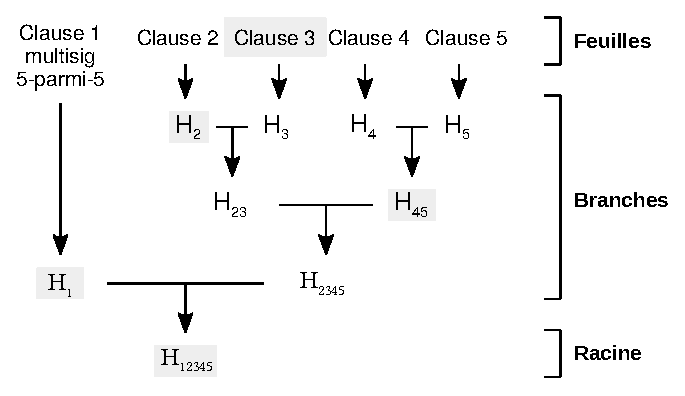
\includegraphics[scale=0.75]{img/taproot-mast.eps}
  \caption{MAST impliquant les clauses d'un contrat.}
  \label{fig:taproot-mast}
\end{figure}

% Historique et supériorité de Taproot
L'implémentation de tels MAST au sein de Bitcoin avait déjà été proposée par le passé, que ce soit sous la forme d'une nouvelle version de SegWit (BIP-114), ou bien d'un nouveau code opération appelé \longstring{OP\_MERKLEBRANCHVERIFY} (BIP-116, BIP-117). Mais Taproot a constitué une proposition supérieure en permettant de ne pas révéler l'existence du MAST lui-même.

% Racine pivot
Taproot inclut en effet une condition de dépense coopérative intégrée. La clé publique agrégée interne est modifiée légèrement (\eng{tweaked}) à l'aide de la racine du MAST, afin de prendre ce dernier en compte. La clé obtenue est celle inscrite dans le script de verrouillage de la pièce, de sorte qu'elle est indiscernable des autres sorties P2TR. De même, la signature agrégée ne peut pas être distinguée d'une signature classique. De ce fait, les participants peuvent dépenser les fonds à l'amiable, tout en étant sûrs qu'un litige mènera au règlement sur la chaîne. % Taproot constitue une façon de régler les contrats en dehors de la chaîne

% RGB
Une alternative à Taproot est RGB, qui est un système de contrats autonomes hors chaîne, construit à la fois en surcouche de Bitcoin et de Lightning. Le nom est issu du standard RGB (\eng{Red Green Blue}) qui permet de définir une couleur et constitue par conséquent une référence directe aux \eng{colored coins}, RGB ayant été originellement conçu comme «~une meilleure version des pièces colorées\sendnote{RGB FAQ, \eng{What does 'RGB' stand for?}, 14 décembre 2020~: \url{https://www.rgbfaq.com/faq/what-does-rgb-stand-for}.}~». Cependant, même si RGB permet effectivement d'émettre et de gérer des jetons, cette fonctionnalité est loin d'être la seule.

RGB se base sur deux primitives techniques conceptualisées en 2016 par le développeur Peter Todd\pagenote{«~deux primitives techniques conceptualisées en 2016 par le développeur Peter Todd~»~: \url{https://petertodd.org/2016/state-machine-consensus-building-blocks\#uniqueness-and-single-use-seals}~; \url{https://petertodd.org/2016/closed-seal-sets-and-truth-lists-for-privacy}.}~: la validation côté client (\eng{client-side validation}) et les scellés à usage unique (\eng{single-use seals}). Cela permet la gestion d'un état indépendant, où la double dépense est empêchée par ces scellés. Après avoir fait l'objet de recherches par Giacomo Zucco et le BHB Network, RGB est actuellement développé par la LNP/BP Standards Association.

% Avantages généraux
L'implémentation de contrats en dehors de la chaîne est donc possible sur Bitcoin, et ils apportent deux choses. D'une part, ils réduisent le paiement de frais en ayant une empreinte minimale sur la chaîne. D'autre part, ils améliorent la confidentialité de leurs participants. C'est pourquoi ils ont le potentiel de jouer un grand rôle à long terme.

\section*{Une monnaie programmable}
\addcontentsline{toc}{section}{Une monnaie programmable}

L'aspect programmable de Bitcoin est souvent négligé. Il n'est en effet pas directement présenté dans le livre blanc, même si Satoshi Nakamoto l'avait déjà élaboré à ce moment-là. Il est toutefois très utile et constitue l'une des facettes essentielles de Bitcoin.

La programmabilité de la monnaie peut servir à contrôler, comme l'illustrent les projets de MNBC qui fleurissent autour du monde. Mais elle peut également rendre un fier service à la liberté individuelle. En effet, cet aspect modulable donne l'occasion à des personnes qui ne se connaissent pas d'échanger de la valeur de la façon la plus sûre possible ou, comme l'exprimait Tim May dans son \emph{Manifeste crypto anarchiste} de 1988, de «~faire des affaires et négocier des contrats électroniques sans jamais connaître le Vrai Nom, ou l'identité légale, de l'autre\sendnote{Timothy C. May, \eng{The Crypto Anarchist Manifesto}, \wtime{22/11/1992 20:11:24 UTC}~: \url{https://cypherpunks.venona.com/date/1992/11/msg00204.html}.}~».

Les contrats autonomes forment la pierre angulaire des relations financières dans le cyberespace. Même la communauté de Monero, qui avait particulièrement restreint cet aspect à des fins de confidentialité, est revenu sur ses pas en intégrant au protocole la fonctionnalité de signature multipartite, notamment dans le but de permettre les échanges atomiques. Une monnaie réellement libre se doit de pouvoir être programmée librement.
% Copyright (c) 2023 Ludovic Lars
% This work is licensed under the CC BY-NC-SA 4.0 International License

\chapter{Le passage à l'échelle}
\label{ch:scalabilite}

% Scalabilité
La scalabilité, calque de l'anglais \eng{scalability}, aussi appelée extensibilité, désigne la capacité d'un système à passer à l'échelle, c'est-à-dire à continuer de fonctionner de manière équivalente à mesure que le nombre d'utilisateurs augmente. Dans un système géré de manière centralisée, cette capacité est assurée par l'apport de matériel informatique, soit en ajoutant de la puissance de calcul à l'infrastructure existante (passage à l'échelle vertical), soit en multipliant les instances de l'infrastructure pour partager le traitement des requêtes (passage à l'échelle horizontal). La scalabilité dépend par conséquent du niveau de prévision de l'entité qui s'occupe du système.

% Système distribué, Bitcoin
Dans le cas d'un système distribué, qui a un comportement différent, la scalabilité se rapporte à quelque chose de plus compliqué. L'ajout de matériel ne suffit pas~: il faut également que les propriétés dudit système se conservent avec la hausse de l'activité. Dans le cas de Bitcoin, ce problème est particulièrement ardu, car toute montée en charge affecte durablement les nœuds du réseau, en raison de la nécessité de partage de la chaîne de blocs intégrale. En substance, le système ne passe pas à l'échelle, ou très peu.

% Débat sur la scalabilité
Ce problème de scalabilité de Bitcoin a été une préoccupation majeure de la communauté, à tel point qu'il a provoqué un véritable conflit ouvert entre 2015 et 2017~: la fameuse guerre des blocs que nous avons décrite dans le chapitre~\ref{ch:clivages}. Certains pensaient qu'augmenter la taille des blocs suffiraient à gérer la demande sans altérer l'offre, tandis que d'autres imaginaient que les solutions de surcouche comme le réseau Lightning seraient assez efficaces pour traiter tous les transferts. Ce chapitre a pour objectif de faire un tour d'horizon de la situation et de proposer une troisième voie.

\section*{L'absence de scalabilité du système} % Non-scalabilité
\addcontentsline{toc}{section}{L'absence de scalabilité du système}

% Vérification de toutes mes transactions
La conception originelle de Bitcoin repose sur un principe simple~: obtenir et vérifier l'intégralité des transactions dans le but de s'assurer qu'il n'y a pas de double dépense. Comme l'écrivait Satoshi Nakamoto dans le livre blanc, «~la seule façon de confirmer l'absence d'une transaction est d'être au courant de toutes les transactions\sendnote{Satoshi Nakamoto, \eng{Bitcoin: A Peer-to-Peer Electronic Cash System}, 31 octobre 2008.}~». De ce fait, pour disposer d'une sécurité maximale, chaque nœud doit, en principe, entretenir une version complète de la chaîne de blocs.

% Message de James A. Donald
Dès les origines, ce fonctionnement particulier a naturellement amené la question de la montée en charge du système. Lorsque Satoshi Nakamoto a présenté sa découverte sur la liste de diffusion dédiée à la cryptographie de Metzdowd.com le 31 octobre 2008, la première réponse qu'il a reçue concernait ainsi ce problème. Cette réponse a était celle de l'ancien cypherpunk James A. Donald le 2 novembre, dans laquelle il écrivait~:

\begin{quote}
«~Nous avons vraiment, vraiment besoin d'un tel système, mais d'après ce que je comprends de votre proposition, il ne semble pas pouvoir s'adapter à la taille requise.

Pour que des jetons de preuve de travail transférables aient de la valeur, ils doivent avoir une valeur monétaire. Pour avoir une valeur monétaire, ils doivent être transférés au sein d'un très grand réseau - par exemple un réseau d'échange de fichiers semblable à bittorrent.

Pour détecter et rejeter un événement de double dépense dans un délai convenable, il faut disposer de la plupart des transactions passées des pièces impliquées dans la transaction, ce qui, mis en œuvre naïvement, exige que chaque pair dispose de la plupart des transactions passées, ou de la plupart des transactions passées qui ont eu lieu récemment. Si des centaines de millions de personnes effectuent des transactions, cela représente beaucoup de bande passante - chacun doit avoir connaissance de toutes les transactions ou d'une partie substantielle de celles-ci.\sendnote{James A. Donald, \eng{Re: Bitcoin P2P e-cash paper}, \wtime{02/11/2008, 23:46:23 UTC}~: \url{https://www.metzdowd.com/pipermail/cryptography/2008-November/014814.html}.}~»
\end{quote} % "We very, very much need such a system, but the way I understand your proposal, it does not seem to scale to the required size.
%
% For transferable proof of work tokens to have value, they must have monetary value. To have monetary value, they must be transferred within a very large network - for example a file trading network akin to bittorrent.
%
% To detect and reject a double spending event in a timely manner, one must have most past transactions of the coins in the transaction, which,  naively implemented, requires each peer to have most past transactions, or most past transactions that occurred recently. If hundreds of millions of people are doing transactions, that is a lot of bandwidth - each must know all, or a substantial part thereof."

% Manque de scalabilité, compromis entre utilité et sécurité
James A. Donald mettait par là en valeur le manque de scalabilité de Bitcoin. Pour tout système donné, une augmentation de volume transactionnel accroît le nombre de transactions à obtenir et à traiter. Cet accroissement rend plus difficile de faire fonctionner un nœud, ce qui peut affecter la décentralisation du réseau et donc la sécurité. De ce fait, il existe toujours un compromis entre l'utilité et la sécurité du système, ou pour mieux le dire, entre la facilité de transaction et la facilité de vérification\pagenote{«~entre la facilité de transaction et la facilité de vérification~»~: Sosthène, \emph{Apologie des petits blocs}, 2 août 2018~: \url{https://www.sosthene.net/apologie-petits-blocs/}.}.

% Limite de capacité transactionnelle, taille limite des blocs
Ce compromis se manifeste généralement par une limite de capacité transactionnelle\pagenote{«~Ce compromis se manifeste généralement par une limite de capacité transactionnelle~»~: Dans le cas où elle n'est définie nulle part, cette limite est de toute manière inférieure à la limite de marché du mineur le plus efficace, car aucun mineur économiquement rationnel ne traiterait de transaction gratuitement.}, décrite par les règles de consensus (limite explicite) ou, plus rarement, par les règles de réseau (limite implicite). La limite de capacité transactionnelle était originellement décrite comme une taille limite des blocs, qui interdisait aux mineurs de créer des blocs plus grands qu'une certaine taille. Dans le prototype, cette taille était définie implicitement par la taille maximale des messages du protocole de transmission, c'est-à-dire 32~Mio. Puis, une limite explicite de 1 mégaoctet (1~Mo) a été ajoutée par Satoshi Nakamoto en septembre 2010 par le biais de la constante \longstring{MAX\_BLOCK\_SIZE}, sans annonce publique de sa part, dans le but d'éviter les attaques par déni de service. Cette taille correspondait, pour un réseau tournant à plein régime, à un volume théorique de 4,5 transactions classiques par seconde, ce qui se ramenait plutôt à 3 transactions par seconde en pratique. % Théorique. P2PKH : 1e2s, 226o (max) ; 2e2s, 374o (max). #tx = 1e6 / (taille_tx * 600) : 1e2s, 7.37 tx/s ; 2e2s, 4,46 tx/s. / Pratique : https://www.blockchain.com/explorer/charts/transactions-per-second

% Poids limite des blocs
Avec l'intégration de SegWit dans la version principale de Bitcoin en août 2017, cette limitation est devenue un poids limite des blocs. Cette nouvelle métrique donnait une importance plus grande de la taille de base par rapport à la taille du témoin dans le calcul de la mesure du bloc, modifiant également la façon dont comptaient les mineurs pour ajouter les transactions au bloc. Cette modification était une augmentation effective de la capacité transactionnelle du protocole, portant le volume autorisé de transactions à 8 transactions par seconde en théorie, et à 4,5 transactions par seconde en pratique. % Théorique. P2WPKH : 1e2s, 223o, 562 wu (max) ; 2e2s, 372o, 834 wu (max). #tx = 4e6 / (poids_tx * 600) : 1e2s, 11.86 tx/s ; 2e2s, 7.99 tx/s. / Pratique : https://www.blockchain.com/explorer/charts/transactions-per-second

% Rareté de l'espace de bloc
L'existence d'une limite de capacité transactionnelle engendre nécessairement une rareté de l'espace de bloc. Si elle est fixe, elle rend l'offre par essence inélastique. Ainsi, une forte demande pour l'espace de bloc fait, par effet d'enchère, augmenter le prix pour l'inclusion, c'est-à-dire les frais de transaction. Le marché des frais est stimulé par cette limite rigide au lieu de rester à son niveau naturel, à savoir celui du coût d'inclusion par défaut des mineurs.

% Plancher d'utilité
Par son effet sur le niveau des frais, la limite crée un plancher d'utilité, c'est-à-dire un niveau de valeur en deçà duquel le transfert et la détention ne sont pas considérés comme rentables par les utilisateurs. En effet, les mineurs sont amenés à rejeter les transactions qui ne paient pas un taux de frais suffisant par rapport à leur taille. De ce fait, l'utilité d'une transaction peut être estimée insuffisante par son auteur au regard du niveau de frais moyen de la chaîne, auquel cas elle n'a pas lieu. Si une personne désire acheter un café pour 2~\$ en BTC, mais que les frais usuels sont de 1~\$, cette personne passera vite son chemin. De manière générale, les cas d'utilisation requérant des frais «~faibles~» sont chassés de la chaîne, à l'instar du service de jeu d'argent SatoshiDICE, qui a dû cesser ses activités sur BTC en 2017 suite à l'augmentation des frais.

% Impact de la limite de capacité transactionnelles sur la décentralisation
La limite de capacité transactionnelle a pour vertu de garantir que le coût d'utilisation d'un nœud reste bas. Elle agit ainsi sur la décentralisation \emph{potentielle} du réseau. En effet, contrairement au matériel minier, le coût lié à la vérification n'est pas compensé par un revenu proportionnel, de sorte qu'il atteint tout le monde de la même manière. Les opérateurs de nœud les moins bien équipés ne peuvent pas matériellement suivre le rythme, ce qui affecte la facilité du réseau à se décentraliser \emph{effectivement}. % Minage : machines de hachage et les mécanismes de refroidissement associés

% Rôle dans le modèle de sécurité
L'influence sur la décentralisation potentielle concerne à la fois le minage et le commerce en empêchant les plus petits acteurs de pouvoir réaliser ces activités à leur échelle. La centralisation du minage augmente le risque de censure, tandis que la centralisation du commerce augmente le risque d'altération du protocole, et donc le risque d'inflation. C'est pourquoi la limite de capacité transactionnelle joue un rôle majeur dans le modèle de sécurité~: moins cette limite est élevée, plus la sécurité \emph{potentielle} du système est grande.

% Limite arbitraire liée à l'interprétation subjective des commerçants
La limite de capacité transactionnelle est déterminée de manière subjective par les commerçants, en fonction de leur \emph{perception de la menace} et de leur \emph{utilisation personnelle} de la chaîne. Il n'existe pas de limite de taille des blocs idéale~: il n'y a que des êtres humains qui calculent un risque par rapport à une éventuelle récompense. On peut tenter d'établir une moyenne pour estimer une limite qui correspond à une utilisation donnée, mais cette estimation serait au mieux imparfaite.

% Plafond d'utilité
Par son effet sur la décentralisation, la limite crée un plafond d'utilité, c'est-à-dire un niveau de valeur au-delà duquel le transfert et la détention sont considérés trop risqués pour la sécurité effective du système. En effet, aucune sécurité n'étant absolue, le transfert et la détention d'une certaine valeur peut ne plus bénéficier suffisamment de la protection apportée par le réseau. Par exemple, recevoir ou conserver l'équivalent de plusieurs millions de dollars sur la chaîne de Bitcoin SV est, c'est le moins qu'on puisse dire, imprudent.

% Plage de valeurs
Le plancher d'utilité (induit par l'action négative de la limite sur l'espace de bloc) et le plafond d'utilité (induit par l'action positive de la limite sur la sécurité) ont pour effet de borner une plage de valeurs en dehors de laquelle le transfert et la détention ne sont plus pertinents\sendnote{Voir Eric Voskuil, «~Propriété du seuil d'utilité~», in \emph{Cryptoéconomie~: Principes fondamentaux de Bitcoin}, Amazon KDP, 2022, pp. 317--318.}. C'est l'existence de cette plage de valeurs qui entraîne l'apparition de substituts à un système donné.

% Non-scalabilité
L'arrivée de nouveaux utilisateurs et l'augmentation subséquente de la demande pour l'espace de blocs rehaussent le plancher d'utilité. Toute montée en charge du système en modifie les caractéristiques. Par conséquent, tout système Bitcoin est en substance non scalable, au sens premier du terme. Il existe cependant des méthodes pour contourner cette absence de scalabilité.

\section*{L'amélioration de l'efficacité de base}
\addcontentsline{toc}{section}{L'amélioration de l'efficacité de base}

% Augmentation progressive de la taille limite des blocs
La première proposition vis-à-vis du passage à l'échelle a été d'augmenter progressivement la limite de taille des blocs dans le but d'accompagner l'accroissement de l'activité\sendnote{Parmi les versions alternatives de Bitcoin, la voie de l'augmentation progressive de la taille limite des blocs a été choisie par Bitcoin Cash, qui prévoit d'intégrer un algorithme permettant de gérer cette augmentation automatiquement. Voir bitcoincashautist, \eng{CHIP-2023-04: Adaptive Blocksize Limit Algorithm for Bitcoin Cash}, 2 septembre 2023~: \url{https://gitlab.com/0353F40E/ebaa/-/blob/f4edacd134103a7e232740463a5f26379bf90f18/README.md}. Elle a également été favorisée de manière plus conservatrice par Monero, qui possède une taille de bloc dynamique basée sur un mécanisme de pénalité pour compenser les \emph{excès} par rapport à la normale. Voir SerHack, \eng{Mastering Monero: The Future of Private Transactions}, Amazon KDP, 2018, pp. 136--139.}\pagenote{«~augmenter progressivement la limite de taille des blocs dans le but d'accompagner l'accroissement de l'activité~»~: Dans Monero, la pénalité ($P$) liée à la taille d'un bloc ($B$) est calculée à partir la taille médiane des 100 derniers blocs ($M$) et la subvention de base ($R$) qui est de 0,6~XMR par bloc depuis 2022. Si $B < M_0 = 300~\mathrm{ko}$, alors $P = 0$. Sinon~:
\[
P = R  \left( \frac{B}{M} - 1 \right)^2~.
\]
La taille du bloc ne peut pas dépasser $2 M$ (taille qui correspond à une pénalité maximale).}. C'était la solution soutenue par Satoshi Nakamoto\pagenote{«~C'était la solution soutenue par Satoshi Nakamoto~»~: Satoshi Nakamoto, \eng{Re: [PATCH] increase block size limit}, \wtime{04/10/2010 19:48:40 UTC}~: \url{https://bitcointalk.org/index.php?topic=1347.msg15366\#msg15366}.}, comme en témoigne sa première réaction à la réponse de James A. Donald le 3 novembre 2008~:

\begin{quote}
«~La bande passante n'est peut-être pas aussi prohibitive que vous le pensez. Une transaction typique est d'environ 400 octets (la cryptographie sur les courbes elliptiques est agréablement compacte). Chaque transaction doit être diffusée deux fois, soit 1 Ko par transaction. Visa a traité 37 milliards de transactions au cours de l'année fiscale 2008, soit une moyenne de 100 millions de transactions par jour. Un tel nombre de transactions nécessiterait 100 Go de bande passante, soit la taille de 12 DVD ou de 2 films en qualité HD, ou encore environ 18~\$ de bande passante au prix actuel. Si le réseau devait atteindre cette taille, cela prendrait plusieurs années, et d'ici là, l'envoi de 2 films en HD sur Internet ne semblera probablement pas être un gros problème.\sendnote{Satoshi Nakamoto, \eng{Re: Bitcoin P2P e-cash paper}, \wtime{03/11/2008, 01:37:43 UTC}~: \url{https://www.metzdowd.com/pipermail/cryptography/2008-November/014815.html}.}~»
\end{quote} % "The bandwidth might not be as prohibitive as you think.  A typical transaction would be about 400 bytes (ECC is nicely compact).  Each transaction has to be broadcast twice, so lets say 1KB per transaction.  Visa processed 37 billion transactions in FY2008, or an average of 100 million transactions per day.  That many transactions would take 100GB of bandwidth, or the size of 12 DVD or 2 HD quality movies, or about $18 worth of bandwidth at current prices. If the network were to get that big, it would take several years, and by then, sending 2 HD movies over the Internet would probably not seem like a big deal."

% Satoshi avait tort
La vision de Satoshi était cependant bien trop optimiste. D'une part, il ne voyait pas la centralisation du minage comme un problème existentiel, prévoyant dès le début que la puissance de calcul du réseau reposerait sur des «~fermes de serveurs composées de matériel spécialisé~». D'autre part, il pensait que la vérification de paiement simplifiée suffirait, ne tenant pas compte de ses défauts de fiabilité et de confidentialité, ni de son incapacité à exercer un pouvoir sur la détermination des règles de consensus. Le plan de Satoshi était donc faillible sans pour autant être entièrement mauvais.

% Facteurs limitants
Le fonctionnement d'un nœud dépend d'un certain nombre de charges. Les principales sont le stockage sur disque dur (HDD) pour l'historique (chaîne de blocs), le stockage en mémoire flash (SSD) pour l'état (ensemble des UTXO), le stockage en mémoire vive (barrette de RAM) pour la réserve des transactions non confirmées (mempool) et la réserve des blocs orphelins, le maintien d'une bande passante (ou débit binaire, usuellement exprimé en Mbit/s) permettant de recevoir et d'envoyer les blocs et les transactions, et le calcul du processeur (CPU) pour la vérification des données et notamment des signatures. Faire diminuer le coût d'un nœud consiste ainsi à réduire l'une de ces charges.

% Optimisation
Même si l'augmentation naïve de la taille limite des blocs ne constitue pas en soi une méthode de scalabilité, il s'avère qu'elle peut être compensée par le progrès technique provenant de l'optimisation logicielle, matérielle ou algorithmique. Premièrement, les performances du logiciel (pour un ensemble donné de règles de consensus) peuvent être améliorées, et il s'agit même de l'une des tâches de base de l'équipe de Bitcoin Core\sendnote{Voir par exemple l'article de Jameson Lopp sur l'évolution de la performance de Bitcoin Core dans lequel décrit comment la première synchronisation sur sa machine s'est améliorée au cours des années. -- Jameson Lopp, \eng{Bitcoin Core Performance Evolution}, 5 mars 2022~: \url{https://blog.lopp.net/bitcoin-core-performance-evolution/}.}. Deuxièmement, le matériel informatique peut être rendu plus efficace, certains composants devenant progressivement moins coûteux (loi de Moore\sendnote{La loi de Moore est une conjecture énoncée par Gordon E. Moore en 1965 ayant postulé que la complexité des semi-conducteurs doublait chaque année. Cette loi était citée par Satoshi Nakamoto dans le livre blanc, qui écrivait~: «~La loi de Moore prédisant une croissance actuelle de 1,2 Go par an, le stockage ne devrait pas poser de problème même si les entêtes de blocs doivent être conservés en mémoire.~» -- Satoshi Nakamoto, \eng{Bitcoin: A Peer-to-Peer Electronic Cash System}, 31 octobre 2008.}). Troisièmement, le protocole peut lui-même être perfectionné au niveau algorithmique, par la découverte et l'adoption de nouvelles techniques plus efficaces~: c'est par exemple le cas de l'algorithme de signature de Schnorr qui produit des signatures plus compactes qu'ECDSA (40~octets au lieu de 72), ou bien des bulletproofs qui rendent les preuves de portée des Confidential Transactions beaucoup moins volumineuses.

% Modifier le comportement du système
Au-delà de ces optimisations, il n'existe pas de manière d'augmenter le volume transactionnel de la chaîne sans faire de compromis au niveau du modèle de Bitcoin. La solution consiste ainsi à modifier le comportement du système, de telle manière qu'il n'affecte pas trop le modèle de sécurité. Plusieurs facteurs peuvent ainsi être optimisés, dont la taille de la chaîne à conserver, l'\eng{Initial Block Download} (IDB) et la taille de l'ensemble des UTXO.

% Taille de la chaîne
D'abord, on peut choisir de supprimer les blocs les plus anciens une fois qu'on les a vérifiés. On conserve simplement la chaîne des entêtes, l'état du réseau, ainsi que les blocs les plus récents afin de pouvoir rejoindre le consensus dans le cas d'une recoordination profonde. Cette méthode est appelée l'élagage ou \eng{pruning}.

% IBD
Mais cette méthode n'enlève pas la charge de l'IBD, c'est-à-dire le processus de téléchargement et de vérification de la chaîne de blocs jusqu'à sa hauteur actuelle. Pour ce faire, on peut procéder à diverses techniques plus ou moins risquées. La première est la supposition de validité des signatures, basée sur le paramètre \texttt{assumevalid}, qui a été introduite dans Bitcoin Core en 2017\sendnote{Bitcoin Core, \eng{Bitcoin Core 0.14.0}, 8 mars 2017~: \url{https://bitcoincore.org/en/2017/03/08/release-0.14.0/\#assumed-valid-blocks}.}, et qui consiste à sauter la vérification des signatures jusqu'à un bloc d'empreinte donnée, faisant gagner beaucoup de temps dans la synchronisation initiale. Cette méthode n'est pas un point de contrôle (elle n'impose pas au bloc d'exister) et le risque qu'elle comporte est minime. La deuxième technique est AssumeUTXO, qui a été proposée en 2019 par James O'Beirne et est toujours en développement\sendnote{James O'Beirne, \eng{AssumeUTXO Proposal}, 24 avril 2019~: \url{https://github.com/jamesob/assumeutxo-docs/tree/2019-04-proposal/proposal}.}, et qui implique de supposer valide un ensemble des UTXO donné (identifié par son empreinte) à une hauteur de bloc déterminée~: l'opérateur de nœud télécharge la sauvegarde de l'ensemble des UTXO auprès d'un tiers et débute la synchronisation initiale à partir de celui-ci, remettant à plus tard (ou ignorant complètement) le téléchargement et la vérification des blocs précédents. Cette méthode présente un défaut de vérification (au moins temporaire) de sorte que l'opérateur est exposé à la tromperie, mais le risque est considéré comme acceptable\pagenote{«~Cette méthode présente un défaut de vérification (au moins temporaire) de sorte que l'opérateur est exposé à la tromperie, mais le risque est considéré comme acceptable~»~: Les risques liées à AssumeValid et à AssumeUTXO sont discutés dans le chapitre~5 de l'ouvrage \eng{Bitcoin: A Work in Progress} de Sjors Provoost publié en 2022.}. Il existe également une troisième technique plus radicale, l'engagement des UTXO (ou \eng{UTXO commitments}), qui est un soft fork obligeant les mineurs à ajouter l'empreinte de l'ensemble des UTXO dans le bloc\sendnote{Mark Friedenbach, \eng{[soft fork] Block v3: miner commitments with compact proofs}, 28 mars 2014~: \url{https://github.com/bitcoin/bitcoin/pull/3977}~; Pieter Wuille, \eng{[bitcoin-dev] Rolling UTXO set hashes}, \wtime{15/05/2017 20:01:14 UTC}~: \url{https://lists.linuxfoundation.org/pipermail/bitcoin-dev/2017-May/014337.html}.}~: cet engagement permettrait de disposer d'une source bien plus fiable pour télécharger la sauvegarde à partir de laquelle commencer la synchronisation.

% UTXO set
Ensuite, au-delà de l'IBD, reste le problème de la taille de l'ensemble des UTXO, qui est l'un des facteurs limitants les plus importants. La première idée pour réduire cette taille est une proposition de Cory Fields appelée UHS (pour \eng{UTXO Hash Set}) qui consiste uniquement à stocker les empreintes (\eng{hashes}) des UTXO individuelles\sendnote{Cory Fields, \eng{UHS: Full-node security without maintaining a full UTXO set}, \wtime{16/05/2018 16:36:35 UTC}~: \url{https://lists.linuxfoundation.org/pipermail/bitcoin-dev/2018-May/015967.html}.}. La deuxième idée est de se servir d'accumulateurs cryptographiques, comme l'a fait Thaddeus Dryja avec sa proposition nommée Utreexo, qui implique de regrouper les UTXO dans des arbres de Merkle afin de condenser l'ensemble à conserver en mémoire, au prix d'un compromis sur la bande passante\sendnote{Thaddeus Dryja, \eng{Utreexo: A dynamic hash-based accumulator optimized for the Bitcoin UTXO set}, 6 juin 2019~: \url{https://eprint.iacr.org/2019/611.pdf}.}. % prononcée «~\eng{U-Tree-X-O}~»

% CISA : Cross-Input Signature Aggregation.

% Sharding
Enfin, on peut également choisir d'éclater le minage et la vérification des transactions en séparant l'historique et l'état du système en plusieurs fragments, qui sont chacun soutenus par une partie (variable) du réseau. C'est ce qu'on appelle le partitionnement ou \eng{sharding}. C'était l'idée derrière l'utilisation d'un arbre préfixe de Merkle-Patricia (aussi appelé arbre Merklix) vaguement envisagée par les développeurs de Bitcoin Cash\pagenote{«~vaguement envisagée par les développeurs de Bitcoin Cash~»~: Amaury Séchet, \eng{Using Merklix tree to shard block validation}, 6 novembre 2016~: \url{http://www.deadalnix.me/2016/11/06/using-merklix-tree-to-shard-block-validation}, archive~: \url{https://web.archive.org/web/20170716220359/https://www.deadalnix.me/2016/11/06/using-merklix-tree-to-shard-block-validation/}~; Joannes Vermorel, Amaury Séchet, Shammah Chancellor, Jason Cox, \eng{Merklix tree for Bitcoin}, juillet 2018~: \url{https://blog.vermorel.com/pdf/merklix-tree-for-bitcoin-2018-07.pdf}.}, ou le \eng{danksharding} qui pourrait être implémenté dans Ethereum\pagenote{«~le danksharding qui pourrait être implémenté dans Ethereum~»~: \url{https://ethereum.org/en/roadmap/danksharding/}.}. Cependant, il s'agit là d'une modification importante du protocole qui pourrait ne jamais être implémentée dans une version de Bitcoin.

%
Ces propositions sont des compromis se faisant au niveau de la chaîne qui affectent souvent le système dans son entièreté. Toutefois, il est également possible de faire un compromis différent, au niveau des pièces individuelles, par l'utilisation de banques et, surtout, de surcouches.

% Toutefois, on peut considérer que le compromis réalisé n'est pas à même de couvrir l'ensemble des plages de valeurs pour traiter l'intégralité de la demande transactionnelle existante...

\section*{Les banques et les surcouches}
\addcontentsline{toc}{section}{Les banques et les surcouches}

Les autres propositions généralement citées comme alternatives à l'augmentation de la taille des blocs sont des solutions consistant à ne pas réaliser tous les transferts sur la chaîne, mais à en déporter les plus petits ailleurs, ceux-ci étant «~regroupés~» dans des transactions plus grosses. La chaîne est alors utilisée pour régler les dettes, contractées de manière analogique (contrat juridique) ou numérique (contrat autonome). Cela consiste à considérer le protocole comme un protocole de règlement.

% La première application dépositaire de ce type était MyBitcoin (2010 - 2011), une interface web permettant un usage facile et serein de Bitcoin, y compris sur mobile.

% Modèle de banque libre
La première manière de faire est de réintroduire de la confiance dans le système en contractant des obligations de manière traditionnelle, auprès de ce que nous appellerons ici des banques. Les banques en question peuvent émettre une monnaie représentative en gardant l'intégralité des fonds, ou bien offrir du crédit en ne conservant que des réserves fractionnaires. L'utilisation de la chaîne sert au règlement entre les banques, qui assure le transfert de fonds entre leurs clients. C'est en somme le modèle de la banque libre promu par George Selgin et Larry White dans les années 1990.

% Hal Finney
Cette première conception a été défendue par Hal Finney, qui avait connaissance des travaux de Selgin et de White, comme nous l'avons vu dans le chapitre~\ref{ch:cybermonnaie}. Le 30 décembre 2010, il faisait ainsi l'apologie d'un modèle de banque libre basé sur le bitcoin~:

\begin{quote}
«~En fait, il existe une très bonne raison pour que les banques basées sur Bitcoin existent et émettent leur propre monnaie numérique, convertible en bitcoin. Bitcoin lui-même ne peut pas passer à l'échelle pour que chaque transaction financière dans le monde soit diffusée publiquement et incluse dans la chaîne de blocs. Il doit y avoir un niveau secondaire de systèmes de paiement, plus léger et plus efficace. [...] Les banques basées sur Bitcoin résoudront ces problèmes. Elles pourront fonctionner comme les banques le faisait avant la nationalisation de la monnaie. Les différentes banques pourront avoir des politiques différentes, certaines plus agressives, d'autres plus conservatrices. [...] Je pense que tel sera le destin ultime du bitcoin, à savoir être la "monnaie de base" qui sert de monnaie de réserve aux banques qui émettent leur propre argent liquide. La plupart des transactions en bitcoin se feront entre banques, pour régler les transferts nets. Les transactions en bitcoin effectuées par des particuliers seront aussi rares que... eh bien, que les achats en bitcoin le sont aujourd'hui.\sendnote{Hal Finney, \eng{Re: Bitcoin Bank}, \wtime{30/12/2010 01:38:40 UTC},\url{https://bitcointalk.org/index.php?topic=2500.msg34211\#msg34211}.}~»
\end{quote}

% Saifedean Ammous
Cette vision a été reprise en 2018 par Saifedean Ammous dans son livre, \emph{L'Étalon-Bitcoin}, dans lequel il soutenait que le rôle principal du bitcoin était d'être une monnaie de réserve\sendnote{«~Bitcoin peut être vu comme un système nouveau et émergent de monnaie de réserve pour les transactions en ligne, dans lequel les banques en ligne émettront des jetons adossés au bitcoin pour leurs utilisateurs, tout en gardant leurs réserves en bitcoins dans un stockage hors-ligne. Chaque individu pourra auditer en temps réel les possessions de l'intermédiaire, et des systèmes de vérification et de réputation permettront de s'assurer qu'aucune inflation n'a lieu.~» -- Saifedean Ammous, \eng{The Bitcoin Standard}, 2018.}. Cette thèse a été par la suite développée par d'autres personnes comme Nik Bhatia\pagenote{«~Cette thèse a été par la suite développée par d'autres personnes comme Nik Bhatia~»~: Nik Bhatia, \eng{Layered Money: From Gold and Dollars to Bitcoin and Central Bank Digital Currencies}, 2021.}. % Andrew Mahowald and Pretyflaco, \eng{The Bullish Case For Bitcoin Custodians}, 12 mai 2023~: \url{https://www.swanbitcoin.com/the-bullish-case-for-bitcoin-custodians/}.

% Places de marché, casinos, institutions
Dans la réalité, cette manière de détourner l'activité de la chaîne s'est effectivement matérialisée avec les places de marché, qui permettaient de traiter les nombreux ordres d'achat et de vente liés à la spéculation. Elle s'est aussi manifestée par le biais des plateformes de casino qui regroupaient les opérations liées au jeu d'argent. Enfin, elle a été mise en œuvre par les services fiduciaires comme Grayscale qui offraient aux institutions financières la possibilité d'intégrer du bitcoin à leur bilan.

% Pas un passage à l'échelle
Toutefois, il ne s'agit nullement d'un passage à l'échelle de Bitcoin. Le traitement bancaire n'est pas résistant à la censure, ni résistant à l'inflation, et sa généralisation conduirait \emph{in fine} à la destruction totale de la proposition de valeur de Bitcoin. Ainsi, on peut vraisemblablement supposer qu'une telle solution ne peut fonctionner qu'à petite échelle, pour des montants modestes, dans la mesure où l'État ne va pas intervenir, comme dans le cas de Bitcoin Beach au Salvador.

% Contrats autonomes, minimisation de la confiance
La deuxième variante de cette solution est de passer, non plus par des contrats juridiques reposant sur la confiance, mais par des contrats autonomes, dans le but de gérer les transferts en dehors de la chaîne. L'idée est ainsi de minimiser la confiance pour rendre le procédé viable. C'était par exemple la démarche derrière les \eng{fidelity bonds}, proposés par Peter Todd en 2013, dont le but était de réduire l'influence du tiers en préservant de la confidentialité financière des clients et en permettant d'auditer efficacement les banques\sendnote{Peter Todd, \eng{Fidelity-bonded banks: decentralized, auditable, private, off-chain payments}, \wtime{23/02/2023 17:49:34 UTC}~: \url{https://bitcointalk.org/index.php?topic=146307.msg1553349\#msg1553349}.}.

% Passage en surcouche
Cette démarche s'est popularisée au moyen de ce qu'on appelle généralement le passage en surcouche (\emph{layering}) qui consiste à déporter l'activité financière vers des protocoles ouverts et décentralisés, préservant partiellement les propriétés de la chaîne. L'idée est de condenser une multitude de transferts en un petit nombre de transactions effectuées sur la couche de base, c'est-à-dire la chaîne de blocs. Cette terminologie est issue de la décomposition en couches de la suite des protocoles Internet, qui est organisée en couches multiples dépendant l'une de l'autre, comme TCP qui dépend de IP. % Analogie imparfaite, Mastercoin / Counterparty correspondent mieux

% Compromis
Dans le passage en surcouche, le compromis de sécurité est partiel (seuls certains bitcoins sont concernés) et limité dans le temps (ces bitcoins peuvent être récupérés sur la chaîne), par opposition au compromis de sécurité total et persistant imposé par l'augmentation de la taille limite des blocs. Il s'agit d'une méthode conforme au modèle à deux couches que Nick Szabo imaginait pour bit gold, avec une couche de base dont le rôle était de garantir la rareté infalsifiable de la monnaie, et une couche supérieure qui permettait de réaliser les paiements effectifs.

% Surcouches
Il existe ainsi une diversité de propositions permettant d'effectuer ce passage en surcouche en réalisant un compromis plus ou moins important. Les principales sont les chaînes latérales, le réseau Lightning et Fedimint, dont nous parlerons en détail par la suite. Il existe également d'autres propositions comme l'échange d'objets physiques (OpenDime\pagenote{«~OpenDime~»~: Les clés Opendime de Coinkite sont les produits les plus réputés pour l'échange physique en dehors de la chaîne. L'utilisateur peut vérifier que le scellé d'une clé n'a pas été brisé et que le contenu de celle-ci correspond au montant indiqué, de sorte qu'il peut l'accepter en tant que moyen de paiement. L'un des inconvénients majeurs est que la perte et le vol sont beaucoup plus faciles que dans le cas d'une portefeuille numérique bien géré. -- Voir \url{https://opendime.com/}.}), le protocole Rumple\pagenote{«~le protocole Rumple~»~: Fiatjaf, \eng{idea: Rumple} \wtime{16/10/2020 21:42 UTC}~: \url{https://fiatjaf.com/rumple.html}.}, les statechains\pagenote{«~les statechains~»~: Ruben Somsen, \eng{Statechains: Non-custodial Off-chain Bitcoin Transfer}, 4 juin 2019~: \url{https://medium.com/@RubenSomsen/statechains-non-custodial-off-chain-bitcoin-transfer-1ae4845a4a39}.}, les ZK-rollups\pagenote{«~les ZK-rollups~»~: Rollkit, \eng{Sovereign rollups on Bitcoin with Rollkit}, 5 mars 2023~: \url{https://rollkit.dev/blog/sovereign-rollups-on-bitcoin-with-rollkit}~; archive~: \url{http://web.archive.org/web/20230511021256/https://rollkit.dev/blog/sovereign-rollups-on-bitcoin/}.} ou encore le protocole Ark\pagenote{«~le protocole Ark~»~: Kudzai Kutukwa, \eng{Introducing Ark: An Alternative Bitcoin Scaling Solution Focused on Preserving Privacy}, 11 juin 2023~: \url{https://bitcoinmagazine.com/technical/how-ark-plans-to-scale-private-bitcoin-payments}.}. % Bitbills, bitcoins de Casascius. Plus tard : Satodime, Satscard.

% condenser une multitude de transferts en un petit nombre de transactions sur la chaîne

\section*{Les chaînes latérales}
\addcontentsline{toc}{section}{Les chaînes latérales}

% --- Chaînes latérales ---

Les chaînes latérales, ou \eng{sidechains} en anglais, sont des chaînes de blocs secondaires fonctionnant parallèlement à une autre chaîne de blocs dite «~principale~». Elles ont été formalisées en octobre 2014 par les développeurs de Blockstream\sendnote{Adam Back, Matt Corallo, Luke Dashjr, Mark Friedenbach, Gregory Maxwell, Andrew Miller, Andrew Poelstra, Jorge Timón, Pieter Wuille, \eng{Enabling Blockchain Innovations with Pegged Sidechains}, 22 octobre 2014~: \url{https://blockstream.com/sidechains.pdf}.}. Cette solution technique apporte une capacité de traitement supplémentaire et une extensibilité supérieure, au prix d'une sécurité locale sensiblement amoindrie. En 2014, Blockstream envisageait de construire ainsi tout un écosystème de chaînes latérales permettant d'accomplir des tâches impossibles sur la chaîne principale comme l'émission d'actifs natifs, le déploiement de contrats autonomes avancés ou la gestion de noms de domaine.

% Image d'illustration du fonctionnement des chaînes latérales présente sur Blockstream.com en octobre 2014\sendnote{Capture du site web Blockstream.com, 25 octobre 2014~: \url{https://web.archive.org/web/20141025021233/https://blockstream.com/}.}

% Ancrage bilatéral
Une chaîne latérale est une chaîne de blocs parallèle à une autre qui permet de transférer des fonds d'une chaîne à l'autre sans mettre en jeu l'intégrité des fonds déplacés. Il s'agit généralement de procéder à un ancrage bilatéral (\eng{two-way peg}) permettant aux bitcoins d'être transférés d'une chaîne à l'autre sans perte de valeur, comme représenté sur la figure~\ref{fig:sidechain-two-way-peg}. Dans un sens, les bitcoins sont verrouillés sur la chaîne principale et leur équivalent est créé sur la chaîne latérale~; dans l'autre, les bitcoins sont détruits sur la chaîne latérale et leur équivalent est déverrouillé sur la chaîne principale

% Maintien de l'ancrage bilatéral
Deux aspects différencient le modèle de sécurité d'une chaîne latérale de celui de la chaîne principale~: le maintien de l'ancrage bilatéral et le mécanisme de consensus. Le premier consiste à décider qui peut déverrouiller les fonds lors d'un transfert de la chaîne latérale vers la chaîne principale. En effet, puisque la chaîne latérale est voulue comme un complément (et pas comme une extension), les nœuds de la chaîne principale n'ont pas connaissance de cette chaîne latérale. De ce fait, le retrait est soumis à une certaine confiance, placée usuellement dans une fédération de participants qui se méfient les uns des autres\pagenote{«~une fédération de participants qui se méfient les uns des autres~»~: Johnny Dilley, Andrew Poelstra, Jonathan Wilkins, Marta Piekarska, Ben Gorlick, Mark Friedenbach, \eng{Strong Federations: An Interoperable Blockchain Solution to Centralized Third-Party Risks}, 2016~: \url{https://blockstream.com/strong-federations.pdf}.}.

\begin{figure}[ht]
  \centering
  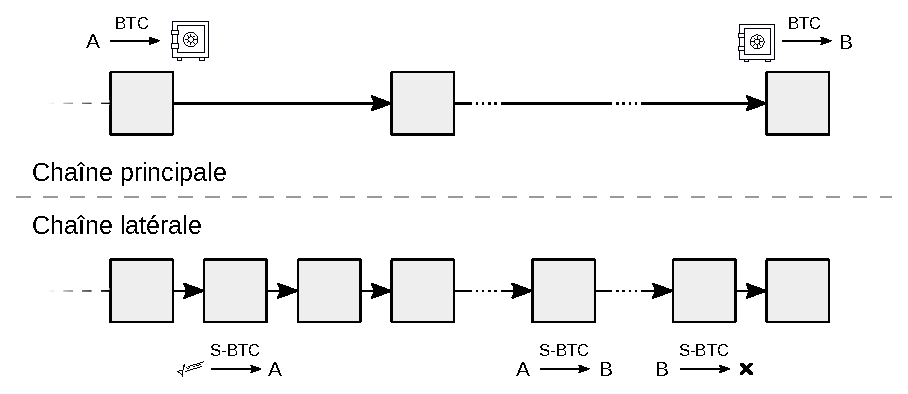
\includegraphics[scale=0.7]{img/sidechain-two-way-peg.eps}
  \caption{Chaîne latérale~: dépôt, transfert et retrait.}
  \label{fig:sidechain-two-way-peg}
\end{figure}

% Mécanisme de consensus
Le second aspect concerne la confirmation des transactions sur la chaîne latérale, et ici les options sont plus variées. Le consensus peut reposer sur le minage combiné, auquel cas c'est le travail de la chaîne principale qui est utilisé. Il peut se fonder sur la preuve d'enjeu, auquel cas c'est l'unité de la chaîne principale qui est impliquée. Ou il peut recourir à une fédération se mettant d'accord grâce à un algorithme BFT classique, auquel cas c'est l'appartenance à cette fédération qui importe (preuve d'autorité).

% Deux chaînes latérales sur BTC
Cette vision s'est concrétisée avec le lancement sur BTC de deux chaînes latérales distinctes en 2018. La première était RSK (aussi appelée Rootstock), qui a été lancée par Sergio Lerner en janvier de cette année-là et qui était focalisée sur l'exécution d'une machine virtuelle Turing-complète s'approchant de celle d'Ethereum. La seconde était Liquid, qui était la mise en œuvre du modèle Elements développé par Blockstream et dont le but primaire était de faciliter les transactions entre les différents acteurs financiers du secteur, dont notamment les plateformes d'échange. Dans Liquid, la sécurité repose sur une fédération de fonctionnaires qui assurent les deux rôles~: ils maintiennent l'ancrage du L-BTC en tant que gardiens (\eng{watchmen}) et participent au consensus de la chaîne en tant que signataires de blocs (\eng{blocksigners}). RSK allie le minage combiné et une fédération de «~notaires~» pour assurer à la fois l'ancrage du RBTC et le traitement des transactions.

% Risques
Les deux chaînes latérales n'ont cependant pas réussi à attirer une activité significative au fil des années, en raison des risques liés. En effet, utiliser ces chaînes requiert toujours une forme de confiance qui, bien que réduite au possible, reste bien présente. Un exemple malheureux d'une sidechain qui a mal tourné est celui de la chaîne latérale SmartBCH de Bitcoin Cash, où la société qui gérait le plus gros pont entre les deux chaînes, CoinFLEX, a fait faillite et n'a pas été en mesure de rembourser les utilisateurs\pagenote{«~la chaîne latérale SmartBCH de Bitcoin Cash~»~: CheapLightning, \eng{The Resolution of the smartBCH Experiment}, 2 août 2022~: \url{https://read.cash/@CheapLightning/the-resolution-of-the-smartbch-experiment-b06eb075}.}.

% --- Drivechain ---

Pour répondre à ces inconvénients et réduire la confiance impliquée, un protocole plus avancé a été élaboré par le chercheur Paul Sztorc depuis novembre 2015~: Drivechain\sendnote{Paul Sztorc, \eng{Drivechain - The Simple Two Way Peg}, 24 novembre 2015~: \url{https://www.truthcoin.info/blog/drivechain/}.}. Comme son nom l'indique (\eng{drive chain} signifie chaîne de transmission), il s'agit d'une véritable machine de création et de gestion de chaînes latérales.

% Ancrage bilatéral est confié aux mineurs
La caractéristique principale de Drivechain est que l'ancrage bilatéral est confié aux mineurs, grâce au dépôt fiduciaire par taux de hachage (\eng{hashrate escrow}) défini dans le BIP-300\pagenote{«~BIP-300~»~: Paul Sztorc, CryptAxe, \eng{BIP-300: Hashrate Escrows}, 23 mai 2017~: \url{https://github.com/bitcoin/bips/blob/master/bip-0300.mediawiki}.}. Durant chaque période de six mois (26~300~blocs), les mineurs votent pour la transaction de retrait de la chaîne latérale distribuant les fonds aux utilisateurs en ayant fait la requête. La transparence et la lenteur de ces transactions permettent à l'ensemble des commerçants de la chaîne principale de les auditer. Les transferts courants, plus rapides, se font par des échanges atomiques ou par des services centralisés.

% Minage combiné « aveugle »
La validation des transactions sur la chaîne latérale utilisant Drivechain peut être assurée par n'importe quel algorithme de consensus. Mais le plus naturel est d'utiliser le minage combiné. C'est pourquoi le projet Drivechain contient également la proposition du minage combiné «~aveugle~» (BIP-301\pagenote{«~BIP-301~»~: Paul Sztorc, CryptAxe, \eng{BIP-301: Blind Merged Mining}, 23 juillet 2019~: \url{https://github.com/bitcoin/bips/blob/master/bip-0301.mediawiki}.}), une technique permettant aux mineurs de la chaîne principale de déléguer automatiquement la validation d'une chaîne latérale à autrui contre une rémunération. Le validateur gagne la différence entre le revenu de la chaîne latérale et l'achat du «~droit de trouver un bloc~». Ceci a pour effet de ne pas obliger les mineurs à gérer les chaînes latérales tout en touchant une partie de leur revenu. % Centralisation du minage à cause du minage combiné ?

% Inconvénients
Drivechain est un concept astucieux qui aurait pour avantage de pleinement réaliser la vision de Blockstream de 2014. Cependant, il présente un inconvénient majeur~: le modèle de sécurité de son ancrage bilatéral. Celui-ci repose en effet sur le recours éventuel à un soft fork réalisé par les commerçants dans le but de corriger une transaction de retrait frauduleuse, qui serait par exemple le fait de mineurs malintentionnés cherchant à voler l'argent du dépôt fiduciaire. Il se fonde donc sur la propension des commerçants à suivre l'activité de la chaîne latérale en question d'une part, et à procéder à une modification du protocole pour geler la transaction incriminée d'autre part. C'est pourquoi cette proposition est, \textcolor{darkgray}{encore aujourd'hui}, largement disputée.

\section*{Le réseau Lightning}
\addcontentsline{toc}{section}{Le réseau Lightning}

% --- Réseau Lightning ---

% Présentation
Le réseau Lightning, ou \eng{Lightning Network} en anglais, est un concept de réseau de canaux de paiements bidirectionnels. Celui-ci a été présenté pour la première fois le 23 février 2015 par Joseph Poon et Thaddeus Dryja lors d'un séminaire de développeurs Bitcoin à San Francisco\sendnote{Taariq Lewis, \eng{SF Bitcoin Devs Seminar: Scaling Bitcoin to Billions of Transactions Per Day}, 5 mars 2015~: \url{https://www.youtube.com/watch?v=8zVzw912wPo}.}. À l'époque, des propositions concurrentes basées sur des idées similaires existaient comme Amiko Pay (conceptualisé par Corné Plooy), Impulse (développé par Jeff Garzik pour Bitpay) et Ström (imaginé par la start-up Strawpay), mais Lightning est rapidement devenu dominant. Il est parfois désigné par LNP/BP (en référence à TCP/IP), car il s'agit de la surcouche favorisée par les utilisateurs de BTC.

% Canaux de paiement
L'infrastructure du réseau Lighning repose sur des canaux de paiement qui sont ouverts et fermés entre des participants. Un canal de paiement est, comme décrit dans le chapitre~\ref{ch:contrats}, un ensemble de contrats autonomes qui permet à deux personnes d'effectuer des paiements répétés de manière sûre et instantanée à partir de liquidités préalablement bloquées. L'utilisation d'un canal est par conséquent limitée par sa capacité, c'est-à-dire la somme des deux soldes des acteurs concernés.

% Fonctionnement de Lightning
Le principe du réseau Lightning est de router les paiements au travers de ces canaux par l'intermédiaire de HTLC, qui sont des contrats d'engagement plus complexes permettant de mettre à jour les canaux concernés\sendnote{En pratique, ces HTLC sont souvent aussi utilisés pour mettre à jour les canaux directement, afin de simplifier la mise en œuvre et d'améliorer la confidentialité. -- Voir Andreas M. Antonopoulos, Olaoluwa Osuntokun, René Pickhardt, «~Routing on a Network of Payment Channels~», in \eng{Mastering the Lightning Network: A Second Layer Blockchain Protocol for Instant Bitcoin Payments}, O'Reilly Media, 2022, pp. 185--207.}. Un paiement transite sur le réseau moyennant des frais minimes qui vont aux nœuds le relayant. Le réseau Lightning est donc semblable à un boulier, dont les tiges sont des canaux et dont les boules sont les satoshis qui transitent d'un côté ou de l'autre des canaux, comme on peut le voir sur la figure~\ref{fig:lightning-network-abacus}.

\begin{figure}[ht]
  \centering
  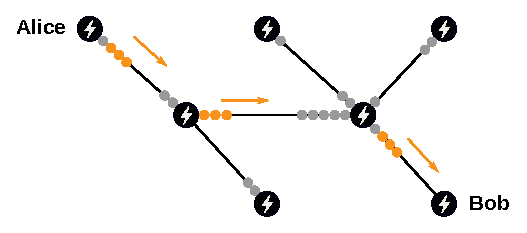
\includegraphics[scale=1.1]{img/lightning-network-abacus.eps}
  \caption{Paiement de 3~mBTC sur le réseau Lightning.}
  \label{fig:lightning-network-abacus}
\end{figure}

% Avantages de Lightning
Ce fonctionnement offre la possibilité de réaliser des paiements quasi instantanés et peu chers. Il permet de faire plus de transferts en bitcoins sans réaliser davantage de transactions sur la chaîne et sans déléguer explicitement la gestion des fonds à un tiers. De plus, le modèle conserve toute la programmabilité de Bitcoin et ouvre le champ des possibles quant à l'utilisation monétaire sur Internet.

% Inconvénients de Lightning
Toutefois, l'apport de Lightning est à nuancer car il n'est pas exempt de défauts. D'abord, il hérite des inconvénients liés au modèle des canaux de paiement où, dans le cas du protocole de Poon-Dryja, une erreur peut mener à la perte des fonds. Puis, les contraintes liées à la capacité et au routage créent nécessairement une tendance à la centralisation, notamment par l'émergence de ce qu'on appelle les \eng{Lightning Service Providers}, ce qui pourrait mener à l'installation d'une certaine censure. Ensuite, contrairement aux idées reçues, la confidentialité sur Lightning est faible, les paiements se faisant entre des clés publiques identifiées et transitant par des intermédiaires. Enfin, le réseau est soumis au niveau des frais sur la chaîne principale, ces derniers étant nécessaires au règlement des contrats, ce qui limite la capacité transactionnelle supplémentaire apportée.

% Pertinence et développement
Le réseau Lightning est donc adapté pour traiter les paiements du quotidien et les micropaiements, ne nécessitant pas forcément la confidentialité et la résistance à la censure offerte par la chaîne de blocs, à partir de canaux bien pourvus et régulièrement réapprovisionnés. Il a été mis en œuvre à partir de janvier 2018, principalement en surcouche de BTC, et s'est développé considérablement depuis, tant d'un point de vue technique qu'économique. Trois implémentations logicielles ont été maintenues par trois entités différentes (lnd par Lightning Labs, c-lightning par Blockstream, eclair par ACINQ) et un système de standards techniques (appelés \eng{Bases of Lightning Technology} ou BOLT) a fini par émerger. Du côté économique, le réseau a rencontré un certain succès en attirant les capitaux et, \textcolor{darkgray}{en novembre 2023, une capacité totale de 5~400~BTC, équivalant à environ 200 millions de dollars}, était réservée pour fournir de la liquidité pour les paiements\pagenote{«~en novembre 2023, une capacité totale de 5~400~BTC, équivalant à environ 200 millions de dollars~»~: \url{https://bitcoinvisuals.com/ln-capacity}.}.

\section*{Les banques chaumiennes de Fedimint}
\addcontentsline{toc}{section}{Les banques chaumiennes de Fedimint}

Une autre proposition est Fedimint\sendnote{Le fonctionnement de Fedimint est décrit dans la documentation présente sur le site web~: \url{https://fedimint.org/docs/intro}.}, qui est un protocole de garde et d'échange confidentiel de bitcoins dans un contexte communautaire. D'un point de vue technique, il s'agit de confier la garde des bitcoins à une fédération et d'échanger des billets chaumiens (eCash) émis par ladite fédération. Ce fonctionnement explique le nom du protocole, qui est une abréviation approximative de \eng{Federated Chaumian Mint} («~monnaierie chaumienne fédérée~» en français).

% Origine
Fedimint a été imaginé par le cypherpunk Eric Sirion au cours de l'année 2021 et implémenté sous forme minimale sous le nom de MiniMint\pagenote{«~MiniMint~»~: Kiara Bickers, \eng{Blockstream Sponsors Federated E-Cash as a Bitcoin Scaling Technology}, 26 octobre 2021~: \url{https://medium.com/blockstream/blockstream-sponsors-federated-e-cash-as-a-bitcoin-scaling-technology-637ba05de7b3}.}. Sirion a été doublement inspiré par les tentatives d'appliquer eCash en surcouche de Bitcoin comme SCRIT\pagenote{«~SCRIT~»~: \url{https://github.com/scritcash/scrit-whitepaper/blob/master/scrit-whitepaper.pdf}.} et par les approches communautaires telles que Bitcoin Beach au Salvador. La première transaction d'une fédération Fedimint a eu lieu le 28 septembre 2022 durant le Hackers Congress de Paralelni Polis.

% --- eCash ---

La première composante de Fedimint est la banque chaumienne qui est gérée par la fédération. Celle-ci utilise le procédé de signature aveugle de David Chaum pour émettre des certificats adossés à un certain montant de satoshis, qui peut être récupéré à tout moment sur la chaîne ou sur le réseau Lightning. Cette composante assure la confidentialité financière partielle des participants~: la banque n'a pas connaissance des échanges réalisés par les clients, mais son rôle de prévention de la double dépense exige qu'elle voie les revenus des commerçants\sendnote{Le fonctionnement technique des systèmes chaumiens a été décrit dans la section «~eCash~: l'argent liquide chaumien~» du chapitre~\ref{ch:cybermonnaie}.}.

% eCash et Bitcoin
L'idée d'utiliser eCash en surcouche de Bitcoin n'est pas une idée nouvelle. Elle a été proposée et implémentée pour la première fois le 17 août 2010, par un individu intervenant sous le pseudonyme fellowtraveller sur le forum de Bitcoin sous la forme de son projet Open Transactions\pagenote{«~Open Transactions~»~: fellowtraveler, \eng{Open Transactions: untraceable digital cash}, \wtime{17/08/2010 20:58:05 UTC}~: \url{https://bitcointalk.org/index.php?topic=847.msg9976\#msg9976}.}. Le projet ne s'est jamais imposé, car le besoin ne se faisait pas ressentir et le système était probablement trop complexe. Cependant, l'idée est revenue timidement sur les devants de la scène au cours du débat sur la scalabilité avec la proposition des «~certificats aveugles au porteur\pagenote{«~certificats aveugles au porteur~»~: theymos, \eng{Blinded bearer certificates}, \wtime{28/12/2016 21:44:24}~: \url{https://www.reddit.com/r/Bitcoin/comments/5ksu3o/blinded_bearer_certificates/}.}~» de Theymos (administrateur du subreddit r/Bitcoin et du forum Bitcointalk) en décembre 2016. Elle a également été reprise en 2019 par Frank Braun et Jonathan Logan (co-animateurs du podcast Cypherpunk Bitstream) au moyen de SCRIT, un projet de système chaumien fédéré dont le nom est l'acronyme de «~\eng{Secure, Confidential, Reliable, Instant Transactions}~». Le dernier projet en date d'une mise en œuvre d'un système chaumien centralisé est Cashu, un protocole développé en 2022 par le développeur callebtc, qui permet la création et l'échange de certificats-bitcoin en surcouche de Lightning et de nouveaux jetons\pagenote{«~Cashu~»~: callebtc sur Twitter, \wtime{14/09/2022 09:47 UTC}~: \url{https://twitter.com/callebtc/status/1569986110272540674}.}.

% --- Approche communautaire ---

L'intérêt de Fedimint, tout comme son prédécesseur SCRIT, est de décentraliser la garde de bitcoins. Pour ce faire, il combine le système chaumien avec une approche dite «~communautaire~», consistant à déployer une banque gérée par les membres de confiance d'une communauté locale.

% Bitcoin Beach
Cette approche a été illustrée par l'expérience de Bitcoin Beach, un projet de développement économique durable autour de la plage d'El Zonte au Salvador. Une banque communautaire a ainsi vu le jour en 2020 et permet depuis lors aux locaux d'échanger des bitcoins de façon sûre et fiable, par le biais du Bitcoin Beach Wallet (devenu Blink) développé par Galoy. C'est cette expérience qui a inspiré l'adoption du cours légal à l'échelle nationale en septembre 2021.

% Fédération
La deuxième composante de Fedimint est donc une fédération, semblable aux fédérations des chaînes latérales comme Liquid ou RSK, mais composée de personnes de confiance qui possèdent les capacités techniques nécessaires à la gestion d'un nœud. Les membres de cette fédération, appelés gardiens, sont responsables de la mise en place de l'infrastructure et se chargent de conserver les fonds des utilisateurs et d'assurer le bon fonctionnement de la banque chaumienne. Ils se coordonnent en utilisant un algorithme de consensus classique (appelé HBBFT\pagenote{«~HBBFT~»~: Il s'agit du sigle de \eng{Honey Badger Byzantine Fault Tolerant}.}) qui, comme tous les algorithmes de ce type, demande un minimum de 66~\% d'acteurs honnêtes pour fonctionner. % Cette composante assure la garde communautaire des fonds.

% Risques
L'emploi de cette fédération représente un compromis technique évident entre la propriété entière des fonds et sa délégation auprès d'un acteur unique. Ce compromis apporte des avantages majeurs au niveau des frais de traitement des transactions et de la facilité d'utilisation, mais engendre également des risques importants. Ceux-ci sont le risque de garde (la fédération peut voler ou perdre des fonds), le risque d'émission frauduleuse (elle peut émettre plus de certificats qu'elle n'a de bitcoins), le risque de censure (elle peut refuser de valider une transaction) et le risque réglementaire (la fédération peut être saisie et fermée sur décision étatique).

% Objectif de Fedimint : prendre le rôle des applications dépositaires
Tout ceci fait que Fedimint ne peut pas être conçue comme une solution de scalabilité, mais comme une proposition de remplacement des applications dépositaires. L'objectif de Fedimint est d'améliorer la garde de bitcoins en la décentralisant et en accroissant la confidentialité des échanges internes. Son caractère local doit permettre d'échapper aux réglementations financières, et ainsi de ne pas subir le sort réservé aux banques classiques.

% La troisième composante est le système d'échanges (atomiques) avec le réseau Lightning. Chaque échange a lieu entre la fédération et un utilisateur par un HTLC. Cela permet la mise en place de passerelles Lightning, qui s'assurent du transfert des fonds depuis ou vers Lightning ou d'autres communautés fédérées pour une aisance d'utilisation optimale. Cette composante assure l'interopérabilité à l'échelle globale entre les communautés.

\section*{Le passage à l'échelle par substitution}
\addcontentsline{toc}{section}{Le passage à l'échelle par substitution}

% Limites des surcouches
Le passage en surcouche est une manière correcte d'accroître le volume économique lié à une chaîne donnée sans trop affecter ses caractéristiques premières. Néanmoins, cette approche présente aussi des limites~: non seulement les différentes surcouches ont leurs défauts propres, mais surtout elles reposent en dernier lieu sur le règlement réalisé sur la chaîne de blocs, dont la capacité est limitée. Par conséquent, le plancher d'utilité n'est pas supprimé par le passage en surcouche et on ne peut ainsi pas voir ce dernier comme un moyen miraculeux de traiter une infinité de transactions.

% Effet de substitution
La plage de valeurs desservie par un système cryptomonétaire donné a pour effet de créer une demande pour des systèmes de substitution plus à même d'assurer le transfert hors de cette plage. Un système dont le niveau de frais est élevé laisse la voie libre à l'utilisation d'un système moins sûr mais moins cher, permettant le traitement des plus petites transactions. À l'inverse, un système dont le niveau de sécurité est faible favorise l'émergence d'un système plus cher mais aussi plus sûr, autorisant les plus gros transferts. Il existe de ce fait une certaine complémentarité entre les différentes mises en œuvre de Bitcoin qui permettent de gérer l'intégralité de l'activité transactionnelle émanant des utilisateurs\sendnote{Eric Voskuil, «~Principe de substitution~», in \emph{Cryptoéconomie~: Principes fondamentaux de Bitcoin}, Amazon KDP, 2022, pp. 315--316.}.

% Complémentarité de l'or et de l'argent
Au cours de l'histoire, une telle complémentarité s'est manifestée par l'utilisation de plusieurs métaux précieux comme base monétaire. L'or ne pouvait pas permettre de couvrir toutes les plages de valeurs~: celui-ci était adapté au transfert de grosses sommes, chose pour laquelle il a été sélectionné comme monnaie de réserve mondiale, mais pas à l'échange de petite monnaie. C'est pour remplir ce dernier rôle complémentaire que l'argent, et d'autres métaux moins précieux comme le cuivre, ont été utilisés. L'argent, mot qu'on utilise encore aujourd'hui en français comme synonyme de monnaie, était la monnaie du quotidien tandis que l'or servait essentiellement aux règlements plus onéreux.

% Bimétallisme
Cet aspect bimétallique (voire trimétallique) de la monnaie a perduré pendant des siècles, de la Haute Antiquité jusqu'au \textsc{xix}\ieme{} siècle. Il était reconnu par les pouvoirs publics qui définissaient leur monnaie comme un poids en or ou en argent, et frappaient des pièces d'or et d'argent en décrétant un taux de change selon le ratio or-argent du marché. On constate d'ailleurs que ce ratio or-argent a été relativement stable au cours de l'histoire en variant entre 10 et 18\pagenote{«~ce ratio or-argent a été relativement stable au cours de l'histoire en variant entre 10 et 18~»~: William Jacob, \eng{An Historical Inquiry Into the Production and Consumption of the Precious Metals}, 1831.}, ce qui confirme le rôle monétaire de l'argent aux côtés de l'or.

% Démonétisation de l'argent
Toutefois, avec l'émergence de l'étalon-or et la disparition du bimétallisme à la fin du \textsc{xix}\ieme{}~siècle, l'argent a peu à peu perdu son rôle monétaire pour être remplacé par la monnaie papier, dans un premier temps adossée à l'or, bien plus commode pour effectuer des échanges. Le ratio a augmenté en conséquence et est passé de 15,5 en 1870 à 80 aujourd'hui, ce qui correspond à une perte de valeur de l'argent de plus de 80~\% par rapport à l'or.

% Litecoin est à l'argent ce que Bitcoin est à l'or
L'analogie avec les métaux précieux est éclairante. Puisque la version principale de Bitcoin (BTC) n'est pas adaptée pour traiter les transferts de plus petite valeur, il s'ensuit que ces transferts potentiels sont réalisés au moyen d'une monnaie de substitution (de la cryptomonnaie, de la monnaie fiat liquide, du crédit déplacé par des services bancaires permissifs, etc.) voire ne sont pas traités du tout. Litecoin, dont la principale narration est qu'il s'agirait d'un argent numérique au même titre que Bitcoin serait un or numérique, répond tout à fait à cette demande. Il était ainsi présenté dès son lancement comme une «~version allégée de Bitcoin~» ayant pour but d'être «~à l'argent ce que Bitcoin est à l'or\sendnote{Charlie Lee, \eng{Re: [ANN] Litecoin - a lite version of Bitcoin. Be ready when is launches!}, \wtime{09/10/2011 06:14:28 UTC}~: \url{https://bitcointalk.org/index.php?topic=47417.msg564414\#msg564414}.}~». Cette désignation ne provient pas tant du fait qu'il y a quatre fois plus de litecoins que de bitcoins, ce qui n'a aucune incidence sur le système, mais plutôt du fait que la capacité transactionnelle maximale de LTC est quatre fois plus grande, ce qui amoindrit la sécurité potentielle du système. Cette analyse vaut également pour Bitcoin Cash à une échelle encore plus grande.

% Services de change, atomic swaps
Dans cette vision, les mises en œuvre alternatives de Bitcoin serviraient à traiter toutes les transactions, au prix de nécessaires transferts entre les chaînes. Ces derniers seraient assurés par des services de change centralisés ou par des systèmes d'échanges atomiques basés sur des carnets d'ordres publics. Cette solution, bien qu'imparfaite, serait tout à fait naturelle et est d'ailleurs déjà pratiquée aujourd'hui.

% Extensivité : confidentialité, programmabilité, noms de domaine
L'extensivité est également concernée par cet effet. Le coût technique d'une utilisation complexe de Bitcoin peut être compensé par des systèmes de substitution de moindre qualité. La confidentialité à bas coût peut être assurée par Monero et la programmabilité simplifiée par Ethereum Classic par exemple. Comme le remarquait très justement Satoshi Nakamoto en décembre 2010, à propos de la pertinence de BitDNS (le futur Namecoin)~:

\begin{quote}
«~Empiler tous les systèmes de quorum par preuve de travail dans une seule base de données ne passe pas à l'échelle. Bitcoin et BitDNS peuvent être utilisés séparément. [...] Les réseaux ont besoin d'avoir des destins différents. Les utilisateurs de BitDNS pourraient être complètement tolérants vis-à-vis de l'ajout de fonctionnalités permettant de traiter des données volumineuses puisque peu de registraires de noms de domaine seraient nécessaires, tandis que les utilisateurs de Bitcoin pourraient devenir de plus en plus sectaires à propos de la limitation de la taille de la chaîne pour que son accès reste facile pour beaucoup d'utilisateurs et pour les petits appareils.\sendnote{Satoshi Nakamoto, \eng{Re: BitDNS and Generalizing Bitcoin}, \wtime{10/12/2010, 17:29:28}~: \url{https://bitcointalk.org/index.php?topic=1790.msg28917\#msg28917}.}~»
\end{quote}

\section*{Trois types de compromis}
\addcontentsline{toc}{section}{Trois types de compromis}

La scalabilité de Bitcoin est un sujet complexe. Contrairement à ce qui est parfois affirmé, un système donné est très peu scalable. Sa capacité à passer à l'échelle ne peut être améliorée qu'au moyen d'optimisations logicielles, matérielles ou algorithmiques. Le gain en performance sur la chaîne se fait la plupart du temps au prix d'un compromis direct, avec l'augmentation de la limite de capacité transactionnelle, ou indirect, avec l'altération du modèle de sécurité.

C'est la raison de l'existence du passage en surcouche, qui consiste à déporter une partie des transferts économiques vers des protocoles ouverts et décentralisés, préservant partiellement les propriétés de Bitcoin et reposant sur le règlement des litiges sur la chaîne. Dans cette démarche, le compromis de sécurité est partiel et limité dans le temps, contrairement au cas de l'augmentation de capacité transactionnelle où il est total et persistant. Le passage de surcouche s'est développé sur BTC au cours du temps par le biais des chaînes latérales, proposées en 2014 et mises en œuvre en 2018, du réseau Lightning, proposé en 2015 et déployé depuis 2018, et de Fedimint, proposé en 2021.

L'autre alternative est le passage à l'échelle par substitution, qui consiste, en substance, à déplacer les transactions les moins à risque vers des substituts de moins bonne qualité, c'est-à-dire des mises en œuvre moins sécurisées du concept Bitcoin. Cet effet s'est réellement manifesté pour la première fois en 2017 avec les premières congestions du réseau BTC et la hausse de la demande pour des contrats autonomes statiques (Ethereum), qui se sont notamment accompagnées d'une baisse de la dominance économique de la version principale de Bitcoin. Les maximalistes ont tendance à prétendre que le passage en surcouche permet de traiter l'ensemble des utilisations pertinentes de Bitcoin, mais, jusqu'à preuve du contraire, ce n'est pas le cas.
% Copyright (c) 2022 Ludovic Lars
% This work is licensed under the CC BY-NC-SA 4.0 International License

\chapter{L'avenir de Bitcoin} % Conclusion et prospective
\label{ch:avenir}

% Bitcoin est un concept de monnaie fiduciaire numérique distribuée, programmable, résistante à la censure et résistante à l'inflation.
% Bitcoin est une révolution conceptuelle, Bitcoin est l'incarnation de la monnaie libre et résiliente, Bitcoin est un moyen élégant et puissant de résister à l'autorité.

La découverte de Bitcoin par Satoshi Nakamoto constitue une révolution conceptuelle profonde dans le domaine monétaire. C'est ce qui explique pourquoi, depuis 2008, il suscite la plus grande passion tant du côté de ses partisans que de ses détracteurs. Certains ont voulu y voir la solution à tous les problèmes de ce monde, une monnaie universelle qui devait remplacer l'or et toutes les monnaies fiat, sans résistance de la part de l'adversaire. D'autres ont tenté de le présenter sous les traits d'un système d'escroquerie organisée, nuisible et pollueur, dans un rejet épidermique souvent lié aux institutions pour lesquelles ils travaillaient.

Dans cet ouvrage, nous avons tenté de faire la part des choses, en décrivant précisément d'où vient Bitcoin, à quels enjeux il répond et quels sont les principes qui le soutiennent. Par sa conception, il constitue un outil d'une rare élégance dont les mécanismes méritent d'être détaillés, ce qui a été fait ici. En guise de conclusion, résumons ce que nous avons développé avant de nous concentrer sur l'avenir de Bitcoin en tant que tel. % menaces qui planent, adoption économique potentielle, culture qui contribue à sa pérennité.

\section*{L'élégance de Bitcoin}
\addcontentsline{toc}{section}{L'élégance de Bitcoin}

% --- Ce que Bitcoin est. ---

% Technique et valeurs
D'abord, rappelons que Bitcoin n'est pas sorti de nulle part. Il est un pur produit de l'évolution technique qui s'est produite dans la seconde moitié du \textsc{xv}\ieme{}~siècle~: il se base largement sur l'ordinateur personnel, sur la cryptographie asymétrique et sur le réseau Internet. Il provient aussi de mouvements idéologiques divers, comme l'agorisme, le librisme ou l'extropianisme, dont la particularité commune était d'appeler à la pratique, de recommander d'agir dans le réel au lieu de se contenter de théoriser. En particulier, il est issu du mouvement des cypherpunks qui, dès le début des années 90, préconisaient d'utiliser la cryptographie de manière proactive en vue de protéger la confidentialité et la liberté des personnes dans le cyberespace naissant. La valeur principale derrière Bitcoin est donc la liberté.

% Cybermonnaie
En outre, il est le résultat d'une longue quête vers la cybermonnaie, qui avait notamment été entreprise par les cypherpunks. Bitcoin doit son existence au système chaumien d'eCash, qui a eu son heure de gloire au milieu des années 90 avant de disparaître. Il s'inspire des tentatives de monnaies numériques privées comme le Liberty Dollar, e-gold et Liberty Reserve, qui ont toutes été arrêtées par l'État au \textsc{xxi}\ieme{}~siècle. Il s'inscrit dans la lignée des concepts de monnaie décentralisée qu'étaient b-money, bit gold, RPOW et, dans une certaine mesure, Ripple.

% Histoire
Bitcoin a été découvert par Satoshi Nakamoto en 2007, qui en a publié le livre blanc descriptif le 31 octobre 2008 avant de finaliser le prototype et de lancer le réseau en janvier 2009. Après des débuts difficiles, la cryptomonnaie a timidement émergée du néant en attirant à elle les personnes intéressées par son potentiel. Ces personnes ont contribué à construire Bitcoin, tant du point de vue du développement informatique, que celui du minage et du commerce. Une fois le projet définitivement lancé en 2010, Satoshi a disparu progressivement et a laissé la main à ses collaborateurs de confiance. Son anonymat demeure complet à ce jour.

% Conflits
Après le départ du fondateur, la communauté a dû s'organiser. C'est à ce moment-là que les premières conférences ont été organisées, que les premières discussions ont eu lieu et que les premiers portefeuilles légers son apparus. Cependant, cette décentralisation du développement de Bitcoin faisait qu'il n'y avait plus un seul point de vue dominant à son sujet, ce qui a mené à de multiples conflits, à commencer par la querelle de P2SH en 2011-2012. Quatre clivages majeurs ont émergé~: le premier concernait la financiarisation, c'est-à-dire la réintroduction partielle de tiers de confiance~; le deuxième se concentrait sur le passage à l'échelle, et le choix de savoir s'il fallait augmenter la capacité transactionnelle de la chaîne ou utiliser des solutions de surcouche~; le troisième gravitait autour du développement des cryptomonnaies alternatives, qui était vivement décrié d'un côté et applaudi de l'autre~; le quatrième se basait sur l'intégration institutionnelle, c'est-à-dire la question de la coopération ou du rejet vis-à-vis de l'autorité. Ces conflits ont fait de Bitcoin ce qu'il est aujourd'hui.

% Nouvelle forme de monnaie
Bitcoin constitue une nouvelle forme de monnaie. Il s'agit d'un intermédiaire d'échange dont la gestion est distribuée, c'est-à-dire qu'elle ne repose pas sur une autorité centrale. Le bitcoin n'est pas une monnaie-marchandise, car ses propriétés ne proviennent pas de caractéristiques intrinsèques du monde physique, même si sa résistance au changement le rapproche des biens tangibles. Ce n'est pas une monnaie scripturale, car les entrées sur son registre ne correspondent pas à des créances, même s'il reprend le caractère numérique du système bancaire. Ce n'est pas une monnaie fiduciaire centralisée, car il ne repose pas sur la confiance placée dans un acteur unique, même s'il n'a pas d'utilisation non monétaire significative. Le bitcoin est une monnaie réticulaire (en référence à son réseau) ou une monnaie fiduciaire distribuée dans le sens où il répartit la confiance sur le réseau de nœuds utilisés par les commerçants plutôt que de la concentrer entre les mains d'une entité unique.

% Proposition de valeur
Bitcoin est un «~système d'argent liquide électronique pair-à-pair~» qui permet «~aux paiements en ligne d'être envoyés directement d'une partie à l'autre sans passer par une institution financière~». Il constitue un concept de monnaie numérique résistante à la censure et à l'inflation, en rendant difficile l'entrave des transactions et la création d'unités supplémentaires. Bitcoin est un outil dont le domaine d'application naturel se situe à la marge, à la limite de la légalité, voire dans l'illégalité. Il est une monnaie de désobéissance utilisée par les activistes politiques, par les lanceurs d'alerte et par les organisations qui s'opposent à l'autorité. Il est une monnaie de la liberté utilisées par les personnes censurées comme celles dont les professions sont jugées déviantes, celles qui font l'erreur d'exprimer une opinion discordante ou celles qui ont eu la malchance de naître dans le mauvais pays. Il est une monnaie du marché noir utilisée par l'économie souterraine, notamment dans le cadre de la résistance fiscale.

% L'Adversaire
Ce statut de monnaie de la liberté fait qu'il s'inscrit dans un rapport antagoniste avec l'État, cette entité toujours plus étendue, qui cherche à affermir son contrôle sur la monnaie dans le but de davantage prélever ses sujets. Par son contrôle sur la banque, il a altéré le support de la monnaie en le faisant reposer sur des billets fiduciaires plutôt que sur des métaux précieux, et il pourrait recommencer en transformant la monnaie physique en une monnaie numérique accessible à tous gérée par une banque centrale. Cette nature prédatrice de l'État est la raison derrière le fonctionnement distribué de Bitcoin, qui est une nécessité. % Le but de l'État est d'institutionnaliser le transfert de richesse non consenti~: il vole ainsi le contribuable par l'impôt, l'épargnant par le seigneuriage et le travailleur indépendant par ses réglementations.

% Propriété
Bitcoin utilise un certain nombre de briques techniques pour fonctionner correctement. La première est la signature numérique qui permet d'assurer la propriété au sein du système. L'utilisateur peut posséder pleinement ses bitcoins par le contrôle sur ses clés privées. Ce mécanisme offre la liberté unique de pouvoir gérer des fonds numériques de manière souveraine, mais demande aussi une certaine responsabilité vis-à-vis de la perte et du vol, qui n'existe pas dans le cadre d'une relation avec un tiers de confiance.

% Confirmation
Pour lutter contre la double dépense, Bitcoin utilise un algorithme de consensus novateur, qui se base sur une chaîne de blocs horodatés de transactions, mise à jour au moyen d'un procédé de preuve de travail. Son fonctionnement ouvert et robuste le distingue des algorithmes de consensus classiques qui avaient été jusqu'alors été mis en œuvre au sein des systèmes distribués. Le génie de Nakamoto est d'avoir sacrifié une partie de la sécurité de l'algorithme (en la rendant probabiliste plutôt qu'absolue) pour assurer la tolérance aux pannes byzantines. Ce modèle repose sur les incitations économiques des mineurs, qui trouvent plus rentable de miner la chaîne dans les règles que de l'attaquer.

% Résistance à la censure
Toutefois, le génie de la conception de Bitcoin ne s'arrête pas là, car celle-ci ne décourage pas seulement la double dépense, mais aussi la censure financière, qui constitue l'un des fléaux du transfert numérique aujourd'hui. La censure de Bitcoin consiste à miner une chaîne plus longue ne contenant pas les transactions indésirables. Grâce au paiement intégré de frais de transactions et au caractère externe de la preuve de travail, une telle censure peut être combattue, ce qui est plus difficile au sein des systèmes sans frais intégrés et des systèmes par preuve d'enjeu (interne).

% Monnaie multiple
Bitcoin est un concept de monnaie ouvert et libre, de sorte qu'il est par nature changeant et multiple. Il existe ainsi une diversité de mises en œuvre de Bitcoin, qui est affectée par deux effets contraires~: l'effet de réseau et l'effet de substitution. Ainsi, la nature monétaire de Bitcoin fait qu'il ne peut que subsister qu'un petit nombre de ces mises en œuvres, tandis que son absence de scalabilité invite à penser qu'il y en aura plusieurs.

% Détermination du protocole ou résistance à l'inflation
La détermination du protocole, ou des protocoles, se fait de manière économique, par l'acceptation des commerçants. Ce sont eux qui, par leur résistance, empêchent l'altération du protocole. Ces commerçants sont bien sûr influencés par d'autres personnes, à commencer par leurs clients, de sorte que le modèle de gouvernance est en réalité bien plus complexe sociologiquement. Les détenteurs, les développeurs, les mineurs, les relais d'opinion, les puissances financières et l'État ont ainsi leur importance dans la prise de décision finale.

% Résistance à l'inflation
La résistance à l'inflation, ou la difficulté à créer plus de bitcoins, émerge de la dynamique économique opposée à l'altération de la politique monétaire. Elle ne provient pas de l'absence d'unanimité de la communauté ou de l'établissement originel de la politique monétaire par Satoshi Nakamoto. La limite des 21~millions, en dépit de son caractère emblématique, n'est ainsi pas absolue et dépend à cahque instant de la décision des commerçants.

% Rouages, confidentialité
Le fonctionnement technique de Bitcoin est optimisé pour la monnaie, comme en témoigne son modèle de représentations des unités qui se base sur des pièces, et non des comptes comme dans Ethereum. Bien qu'aucune technique avancée n'ait été intégrée dans le prototype, Bitcoin est également conçu pour être confidentiel, la confidentialité étant nécessaire pour la fongibilité de la monnaie et sa résistance à la censure.

% Programmabilité
De plus, Bitcoin est programmable, de sorte qu'il est possible d'imposer des conditions de dépense à différentes pièces. Cet aspect modulable des transactions donne la possibilité à des inconnus d'échanger de la valeur de manière la plus confidentielle et sûre possible. Il est aussi à la base des protocoles de surcouche, comme le réseau Lightning, qui augmentent la capacité de traitement des échanges sans compromettre la sécurité du système de base.

% L'élégance de Bitcoin
Toutes ces propriétés de Bitcoin forment un tout cohérent d'une rare élégance. Bitcoin constitue la pièce manquante du puzzle de liberté sur Internet. Bitcoin représente l'espoir d'une génération face à l'autorité étatique grandissante. Bitcoin incarne le projet d'un système monétaire alternatif robuste et durable. C'est ce qui explique le formidable élan qui l'a accompagné dans les premières années.

%  Il circule tout un tas de théories plus ou moins fausses au sujet de Bitcoin que cette description suffit à invalider. Toutes ces théories ne font qu'affaiblir Bitcoin face aux vraies menaces qui pèsent sur lui.

\section*{Les quatre menaces qui planent sur le système}
\addcontentsline{toc}{section}{Les quatre menaces qui planent sur le système}

Comme nous l'avons évoqué tout au long de cet ouvrage, Bitcoin n'est pas à l'abri de subir des attaques. Nous ne parlerons pas des menaces techniques, bien réelles bien que parfois exagérées, que des personnes mieux informées ont déjà traitées\sendnote{Voir par exemple Sjors Provoost, \eng{Bitcoin: A Work in Progress}, 2022.}. Nous décrirons ici uniquement les menaces émanant de l'action des acteurs économiques du système, qui sont pour nous bien plus importantes.

% Menaces subtiles
Ces menaces sont subtiles, car les attaques qu'elles facilitent surviennent généralement de manière soudaine. L'accroissement de ces menaces est similaire à une sorte de jeu de chaises musicales, où les participants tournent naïvement autour des chaises sans les surveiller. Tant que la musique retentit dans la pièce, tout va bien~: l'adversaire enlève les chaises une par une, calmement, mais la ronde continue. C'est au moment où la musique s'arrête que les problèmes commencent.

% Quatre menaces
Nous distinguons quatre menaces de ce type qui sont susceptibles de nuire à Bitcoin~: la centralisation de l'activité économique, la centralisation de l'activité minière, la généralisation de la garde de fonds et l'effacement de la confidentialité. Celles-ci ne sont pas entièrement indépendantes, mais elles correspondent chacune à un comportement différent des acteurs.

% Attaque d'altération du protocole
La première menace est la centralisation de l'activité économique, qui advient au travers du commerce important réalisé auprès des plateformes de change réglementées et par le recours quasi systématique à des processeurs de paiement externes et à des fournisseurs de portefeuille tiers. Celle-ci peut mener, comme nous l'avons décrit dans le chapitre~\ref{ch:determination}, à une attaque d'altération du protocole, sous la forme d'un hard fork d'inflation, d'un soft fork taxatoire ou d'un soft fork de censure. Il est probable que cette attaque crée une scission d'une façon ou d'une autre. Elle est spécialement dommageable dans le cas où la chaîne altérée est majoritaire en raison de l'effet de réseau. Cette attaque n'est néanmoins pas fatale pour le système car l'économie peut se reconstruire progressivement à partir de la chaîne libre.

% Attaque de censure des transactions
La deuxième menace est la centralisation de l'activité minière, qui se manifeste notamment par le rapprochement géographique du matériel de minage, par le regroupement des hacheurs en coopératives et par l'utilisation collective de relais centralisés par les mineurs. Ce risque peut mener, comme vu dans le chapitre~\ref{ch:censure}, à une attaque de censure des transactions par la majorité de la puissance de calcul du réseau. Cette attaque arrive logiquement après la tentative d'altération du protocole et se produit sur la chaîne libre. Elle a pour effet de paralyser une partie de l'activité en empêchant sa confirmation sur la chaîne. Elle bénéficie de l'analyse de chaîne qui lui permet d'isoler les transactions problématiques plutôt que de supprimer l'intégralité de l'activité. Elle n'est cependant pas mortelle pour le système, car du matériel de minage supplémentaire peut être déployé, suite à l'accroissement des frais des transactions censurées, pour restaurer la situation initiale. % La communauté pourrait cependant mal réagir pour contrer la censure en modifiant le protocole à court terme, ce que le minage a pour vocation d'éviter.

% Généralisation de la garde de fonds
La troisième menace, apparentée à la centralisation de l'activité économique, est la généralisation de la garde de fonds par des dépositaires qui suivent les réglementations légales. Non seulement cette pratique n'est pas pertinente du point de vue individuel (un dépositaire peut censurer les transactions, saisir les fonds et gonfler la quantité de bitcoins-papiers qu'il distribue), mais sa généralisation crée aussi un risque au niveau systémique. Cette menace se manifeste aujourd'hui par le développement de dépositaires institutionnels comme Coinbase Custody qui détiennent un pourcentage non négligeable des bitcoins en circulation\sendnote{\url{https://platform.arkhamintelligence.com/explorer/entity/coinbase}, \url{https://twitter.com/brian_armstrong/status/1595126425371414528}}. Elle est plus dangereuse que la centralisation de l'économie, car l'économie «~hébergée~» ne peut pas se reformer s'il y a une attaque contre le protocole~: ce sont les dépositaires réglementés qui sont les réels propriétaires des bitcoins, pas leurs clients. Il s'agit donc d'une dégénérescence persistante du système, qui se résorbe plus difficilement qu'une simple centralisation minière ou commerciale.

% Confidentialité
La quatrième menace, plus subtile, est l'effacement de la confidentialité, qui se matérialise par la surveillance généralisée (connaissance du client, preuve de propriété d'adresse) et, accessoirement, par l'analyse de chaîne qui l'accompagne. À l'instar de la garde de fonds par une entité réglementée, la complète transparence vis-à-vis de l'État constitue non seulement un errement individuel (la personne n'est protégée ni de la censure, ni de la saisie), mais aussi un risque systémique dans le cas où elle se généralise. En effet, une surveillance plus grande crée une économie davantage contrôlable, et rend par conséquent le protocole plus vulnérable. En outre, l'identification des acteurs a pour conséquence de réduire l'ensemble d'anonymat qui profite à tout le monde, et de diminuer la possibilité d'exercer une activité de manière confidentielle. L'effacement de la confidentialité forme ainsi une dégénérescence subtile du système, qui ne peut être guérie que par la lutte contre les liens d'identification \emph{via} l'application de bonnes pratiques. % Par la progression de la propreté, Bitcoin se désintègre. Bitcoin est sale par nature, car Bitcoin est vivant, Bitcoin se roule dans la boue, Bitcoin est un rat d'égoût.

% Que faire ? Adoption plus saine
Ces menaces dépendent des actions des acteurs économiques de Bitcoin, et notamment de ses utilisateurs. Pour combattre ces menaces, il convient donc de pousser les utilisateurs à retirer leurs bitcoins sur un portefeuille, à arrêter de se soumettre à la connaisance du client, à mélanger leurs bitcoins pour les rendre intraçables et à utiliser leurs propres nœuds, individuels ou communautaires. Cela concerne en particulier les nouveaux utilisateurs, ce qui nous amène au thème de l'adoption.

\section*{Les deux adoptions de la cryptomonnaie}
\addcontentsline{toc}{section}{Les deux adoptions de la cryptomonnaie}

Bitcoin est un système basé sur des incitations économiques, dans lequel les personnes qui le font vivre sont récompensés. D'une part, les mineurs sont incités à confirmer les transactions pour toucher les frais de transactions. D'autre part, les commerçants sont incités à vérifier les règles de consensus pour bénéficier en toute quiétude de la proposition de valeur de Bitcoin. Et en outre, les détenteurs sont incités à promouvoir Bitcoin pour agrandir l'économie et profiter de la hausse résultante du pouvoir d'achat (ou du prix en dollars) de l'unité de compte. Cet agrandissement de l'économie est aussi appelé l'adoption, et il est logique qu'elle constitue l'un des objectifs naturels de ceux qui possèdent du bitcoin.

% Deux modèles d'adoption
L'adoption de Bitcoin peut avoir lieu de multiple manières, mais deux modèles principaux se distinguent. Le premier est l'adoption par les individus et par les petites entreprises, qui correspond à un apport financier modeste à la valeur agrégée du bitcoin. Le second est l'adoption par les grandes entreprises, par les sociétés de courtage et par les institutions financières, qui peut constituer un plus gros gain pour les détenteurs. Dans les premiers temps, il était impossible de convaincre cette dernière catégorie du bienfondé du bitcoin, mais avec le développement économique et avec l'aseptisation de la communication, il est devenu aujourd'hui bien plus aisé de la persuader d'y participer. Puisque cette adoption était beaucoup plus rentable pour les détenteurs, beaucoup d'entre eux ont choisi la voie de la facilité en remplissant leur discours d'éléments de langage destinés aux acteurs réglementés.

% Mauvais adoption
Mais cette seconde adoption du bitcoin, bien qu'elle soit certainement rentable sur le moment et qu'elle possède des mérites propres, devient stérile à long terme. En effet, elle crée une économie centralisée, surveillée voire entièrement dépositaire, c'est-à-dire une économie fragile à la merci des décisions étatiques. C'est pourquoi on peut la qualifier de mauvaise adoption.

% Bonne adoption
Ainsi, la seule adoption à laquelle il vaut la peine de s'intéresser est celle de l'économie libre et indépendante, pour laquelle Bitcoin est adapté en premier lieu. Cette économie possède en effet les caractéristiques qui permettent à Bitcoin de perdurer. Elle est décentralisée et répartit les risques entre tous ses membres, pour bénéficier au maximum de la proposition de valeur de Bitcoin. Elle est désobéissante, dans le sens où elle refuse toute modification du protocole qui altérerait les propriétés fondamentales de Bitcoin. Elle protège sa confidentialité, car elle sait qu'elle a quelque chose à craindre de ceux qui la surveillent. Elle est circulaire, au sens où elle évite le plus possible le recours à la monnaie étatique, surtout sous sa forme numérique, car elle sent que cette dernière est de plus en plus surveillée et contrôlée. Enfin, elle est exigeante, en demandant de l'individu un certain discernement et une certaine responsabilité, des qualités trop souvent négligées à notre époque moderne.

% L'adoption de masse n'aura pas lieu
Toutefois, les contraintes de cette adoption font qu'elle n'est pas accessible à tous. Non seulement l'utilisation souveraine de Bitcoin demande d'être un minimum responsable, mais elle présente aussi des inconvénients majeurs, qui sont (à l'heure actuelle) la volatilité du pouvoir d'achat, le coût de transaction, le manque de scalabilité et la réglementation dissuasive. De ce fait, il est difficile d'envisager que tout le monde fera du bitcoin sa monnaie de prédilection à court ou moyen terme. Pour le dire autrement~: l'adoption de masse n'aura pas lieu, et Bitcoin restera probablement un outil utilisé par la partie de la population qui cherche à s'extraire du système et à résister aux puissances de ce monde.

% Délusion
Il est donc illusoire de s'attendre à une «~hyperbitcoinisation\sendnote{Daniel Krawisz, \eng{Hyperbitcoinization}, 29 mars 2014~: \url{https://nakamotoinstitute.org/mempool/hyperbitcoinization/}~; Pierre Rochard, \eng{Speculative Attack}, 4 juillet 2014~: \url{https://nakamotoinstitute.org/mempool/speculative-attack/}.}~», c'est-à-dire à un remplacement des monnaies fiat par le bitcoin. Tant qu'il y a une masse de gens qui continuera d'obéir aveuglément au pouvoir, la monnaie étatique subsistera. Seule la nécessité pourra pousser les masses à faire un usage opportuniste et temporaire de Bitcoin.

\section*{Une culture en gestation}
\addcontentsline{toc}{section}{Une culture en gestation}

% Définition de la culture
La culture est l'ensemble des aspects matériels, intellectuels, affectifs et spirituels, qui caractérisent une société ou un groupe social\sendnote{«~Dans son sens le plus large, la culture peut aujourd'hui être considérée comme l'ensemble des traits distinctifs, spirituels et matériels, intellectuels et affectifs, qui caractérisent une société ou un groupe social. Elle englobe, outre les arts et les lettres, les modes de vie, les droits fondamentaux de l'être humain, les systèmes de valeurs, les traditions et les croyances.~» -- UNESCO, «~\emph{Déclaration de Mexico sur les politiques culturelles}~», \emph{Conférence mondiale sur les politiques culturelles}, 26 juillet -- 6 août 1982~: \url{https://www.culture.gouv.fr/Media/Thematiques/Egalite-et-diversite/College-de-la-Diversite/Declaration-de-Mexico}.}. Chaque association humaine durable a tendance à développer une culture propre. La communauté de Bitcoin, bien que vaguement délimitée, n'échappe pas à ce phénomène. Des éléments culturels ont émergé dans Bitcoin dès ses débuts et, à mesure que le réseau grandissait, ces éléments se sont multipliés pour former un ensemble complexe, menant à la naissance d'une véritable \eng{subculture}.

% La culture de Bitcoin
Cette culture est logiquement pétrie de politique, allant de l'animosité à l'égard de l'autorité et de ses représentants, aux références multiples à l'école autrichienne d'économie. Elle est aussi constituée de pratiques monétaires ritualisées, de recommandations hygiéniques à l'encontre des crypto-actifs douteux, d'œuvres d'art futuristes, de livres et de podcasts en tous genres, de regroupements lors de rencontres mensuelles et de conférences et de dates de commémoration. La culture de Bitcoin, conformément à sa nature de monnaie d'Internet, repose aussi beaucoup sur des formules courtes répétées à foison et sur des mèmes humoristiques.

% Culture et comportement
La culture, et plus précisément la part de la culture que l'on pourrait qualifier de religieuse\sendnote{«~Une religion est un système solidaire de croyances et de pratiques relatives à des choses sacrées, c'est-à-dire séparées, interdites, croyances et pratiques qui unissent en une même communauté morale, appelée Église, tous ceux qui y adhèrent.~» -- Émile Durkheim, \emph{Les formes élémentaires de la vie religieuse}, 1912.}, a pour conséquence d'orienter les actions des individus. Puisque Bitcoin est un outil dont l'efficacité dépend de l'utilisation qui en est faite, cet aspect culturel est fondamental. Par exemple la phrase «~\eng{not your keys, not your bitcoins}~» inventée par Andreas Antonopoulos vaut bien plus que toute explication technique des portefeuilles ou tout exposé historique des faillites de dépositaires. Mais la culture peut aussi, par une mauvaise orientation, induire de mauvais comportements et finalement nuire au système. % Bitcoin a ainsi un problème de culture.

% Aspect spéculatif de Bitcoin
En tant qu'objet spéculatif dont le prix a été multiplié par 30~millions en l'espace de 14 ans, le bitcoin a attiré les personnes avides de gains financiers. Le bitcoin bénéficiant d'une rareté absolue par conception, ce qui ne s'était jamais vu dans l'histoire, il était normal qu'il en soit ainsi. C'était là l'un des choix essentiel de Satoshi Nakamoto, car cet attrait spéculatif a permis en partie d'amorcer le processus de monétisation et de faire découvrir Bitcoin à des personnes qui s'en seraient sinon détournées.

% Avarice
Mais la culture de Bitcoin en a aussi été profondément été influencée, ce qui a contribué à créer une réelle tendance à l'avarice au sein de Bitcoin. Il y a ainsi l'idée que le nombre, c'est-à-dire le prix en dollars, doit monter (\eng{number go up}), qu'il doit être propulsé «~jusqu'à la lune~» (\eng{to the moon}) en vertu du fait que la richesse du monde est infinie et qu'il n'y a que 21 millions de bitcoin ($\infty / 21$\sendnote{Knut Svanholm, \eng{Bitcoin: Everything divided by 21 million}, 2022}). Par conséquent, l'individu doit accumuler des satoshis (\eng{stack sats}) et les thésauriser (HODL\sendnote{GameKyuubi, \eng{I AM HODLING}, \wtime{18/12/2013 10:03:03 UTC}~: \url{https://bitcointalk.org/index.php?topic=375643.msg4022997\#msg4022997}~; Coindesk, \eng{Maybe Don't HODL Bitcoin... – Hodl Guy}, 11 janvier 2019~: \url{https://www.youtube.com/watch?v=6lAPU2yP6rw}.}) dans le but de profiter d'une vie meilleure. Cet aspect se retrouve dans les représentations de Bitcoin et des bitcoineurs, comme le taureau du marché haussier\sendnote{Vijay Boyapati, \eng{The Bullish Case for Bitcoin}, 2021.} ou bien les yeux laser (\#LaserRayUntil100K). % Citadelles. «~1 BTC~=~1 BTC~».

% Adoption de masse
Cette volonté d'obtenir un niveau de prix toujours plus haut repose sur la délusion de l'adoption de masse que nous avons évoqué ci-dessus. Pour que le prix atteigne les sommets, il faut en effet que tout le monde finisse par posséder du bitcoin d'une manière ou d'une autre. Comme la plupart des gens ne sont pas prêts à utiliser Bitcoin de manière souveraine, cette adoption s'est faite au travers de dépositaires. De ce fait, la culture basée sur le gain financier a conduit l'affaiblissement subtil de Bitcoin par l'acception de l'installation généralisée d'intermédiaires financiers, par le consentement à l'identification de masse et par la promotion de l'adoption auprès des institutions et des États. % Même si le gain financier n'est pas antithétique à Bitcoin en tant que tel, il le devient lorsqu'il altère son modèle de sécurité.

% Vocation d'Isaïe
L'adoption de masse n'est pas un objectif réaliste ni à court, ni à moyen terme. Lorsque nous vantons les avantages de Bitcoin, nous ne nous adressons pas à la masse proprement dite~; nous nous adressons au reste, aux quelques uns qui comprennent les tenants et aboutissants des problèmes qu'il permet de résoudre et qui sont susceptibles d'être intéressés\sendnote{Albert Jay Nock, \eng{Isaiah's Job}, 1936~: \url{https://www.theatlantic.com/magazine/archive/1936/06/isaiahs-job/652293/}.}. C'est pourquoi il est essentiel de ne pas aseptiser le propos~: pour ne pas perdre ces personnes, il faut dire la vérité. Et si cette vérité peut être voilée, elle ne doit jamais être déformée. % Nous ne nous adressons pas aux détracteurs. Les détracteurs, qui travaillent pour l'adversaire, existeront toujours. S'il est utile de se confronter à eux pour rétablir la vérité (notamment devant un public qui doute), il l'est aussi de se préparer dûment aux épreuves que Bitcoin ne manquera pas de subir.

% Adoption partielle
Bitcoin a pour vocation d'être toujours partiellement adopté et menacé. Dès que l'opinion publique approuve pleinement les valeurs apportées par Bitcoin, la monnaie légale s'assainit et la contrainte de sécurité de Bitcoin n'est plus nécessaire. Bitcoin vit par conséquent de la tension qui existe entre l'économie officielle, qui approuve le pouvoir sur la monnaie, et la contre-économie, qui s'y oppose.

% Construction d'une tradition
Du fait de cette tension, la culture de Bitcoin est également constamment attaquée, notamment par les médias de masse, par les banquiers centraux et par les représentants de l'État. Il existe ainsi un nombre stupéfiant de détracteurs qui, travaillant pour l'adversaire\sendnote{«~Il est difficile de faire comprendre quelque chose à un homme lorsque son salaire dépend précisément du fait qu'il ne la comprenne pas.~» -- Upton Sinclair, \eng{I, Candidate for Governor, and How I Got Licked}, 1934.}, répètent à l'envi leur argumentaire de mauvaise foi. S'il est utile de se confronter à eux pour rétablir la vérité devant un public qui doute, il est vain de croire qu'ils disparaîtront ou perdront en visibilité. C'est pourquoi Bitcoin a besoin d'une tradition, d'une transmission culturelle d'individu à individu, qui permettrait d'expliquer ses principes de manière saine et organique au nouveau venu. % "It is difficult to get a man to understand something when his salary depends upon his not understanding it."

% Proactivité
En particulier, le message de Bitcoin devrait être un appel à la pratique, conformément à ce qu'ont répété les mouvements idéologiques dont il est issu, à commencer par les cypherpunks. Chacun devrait se sentir poussé à écrire (et à lire) du code, à déployer des fermes de minage dans la mesure du possible, à participer à l'économie circulaire (ce qui implique de conserver du bitcoin), à éduquer sur le fonctionnement des portefeuilles et à faire mille et une choses pour faire progresser la compréhension au sujet de la cryptomonnaie. Car c'est aussi de cette manière que Bitcoin prospère.

% Conclusion
Quoi qu'il en soit, Bitcoin ne peut pas être oublié. La découverte de Satoshi Nakamoto est là pour rester. Elle a déjà joué un rôle dans le combat pour la liberté humaine et devra probablement jouer un rôle encore plus grand à l'avenir. Son succès dépendra de l'action des personnes qui le soutiennent.

% \backmatter

\printendnotes

\end{document}